\section*{搯 3 㙱}
\section*{3.1 论争、言辞攻争与定义}
3.2 定义的类型和论争的解决\\
3.3 外延和内涵\\
3.4 外延定义\\
3.5 内涵定义\\
3.6 属加种差定义的规则

第3章概要

\section*{3.1 论争、言辞之争与定义}
语言是一种非常复杂的设施,是人类最重要的交流工具。但是,当语词被漫不经心或错误地使用时,这种设施就会变成我们的负担。在 2.5 节中,我们阐释了冲突双方的歧见既可能是信念的也可能是态度的;而我们看到,两者之中任何一种对立都可能是实质歧见。但是,也存在这样的情况:表面上的歧见实际上却不是真正的歧见,而仅仅是误解或词汇误用的结果。在前一章中,我们考察了不同类型的实质歧见;在这里,我们转而讨论不同类型的论争,分辨其是否具有真正的分歧。

必须区分出三种不同的论争。第一种是明显的实质论争,在这种论争中,各方或者在信念上或者在态度上,明确地毫不含糊地对立。例如,如果美国佬(Yankees)赢得了世界联赛,虽然在胜利者本身的认同上没有争论,但如果 A 为此高兴而 B 为此恼怒,那么他们的态度歧见(不可能解决的问题)就是显然的,或许甚至是激烈的。在另一种语境中,如果 A坚持认为巴拿马运河的太平洋人口比其大西洋人口更靠东,而 B 则否定如此,那么他们的争论就不是在态度上而是在事实上;而一张好地图就可以平息这个论争。 ${ }^{[1]}$ 无论是态度上的还是信念上的,这种论争总是包含某种实质歧见。将论争双方区别开来的不仅仅是语言,在他们对事实的断定上或对事实的评价上亦存在实质差别。因此,这样的实质论争不能通过定义或任何简单的语言调整来解决。

当然,可以存在关于词汇本身的实质论争,例如,某个单词怎样拼写或者怎么使用;也可以存在关于态度本身的实质论争,例如,是否某第三方不友好或仅是差怯。事实可以是物理的或地理的,也可以是语言的或心理的,而且各方可以在任何种类事实上产生歧见。但是,如果论争确实是关于某个事实的,那么它就是实质的,并可以通过确认某些事实而得到解决。

然而,也存在第二种类型的论争,即纯粹的言辞之争;在这种论争中,双方之间根本没有实质歧见,然而却好像是具有歧见。语言的误解或误用可能是这里的症结所在。当论争者的信念表达中某个关键语词有歧义,而这种歧义又遮蔽了双方并没有实质对立的情况时,言辞之争就会产生。若争论某方误用一个重要词语,或者争论的某个核心语词或短语具有

不同含义,而这些含义可能同等合法但产生了不应有的混淆,或者由于各方对语词或短语的用法都对但含义不同,而这一点又没有被明确认知,就可能产生这种表面的言辞之争。

言辞之争并非总是容易发现,但一旦识别了它,通过具体化歧义语词或短语的不同含义,就可以相当容易地获得解决。在这种语境中,良好的定义对相互理解是非常关键的。

威廉•詹姆士给出了这种言辞之争的一个经典例子:

几年前,我随野营队一起在山上露营。当我独自散步返回时,发现每个人都参加了一场激烈的形而上学论战。争论主题是一只松鼠。设想一只松鼠抓附在树干一侧,而一个人站在树的另一侧;那人绕树迅速转动以试图看到松鼠,但无论他转多么快,松鼠在相对的方向都以同样快的速度转动,在它自己和那人之间总隔着那棵树,因此使他看不到松鼠。作为结果的形而上学问题是:这个人是否绕着松鼠走了一圈?确确实实,他绕树走了一圈,而且松鼠就在树上;但是,他绕松鼠走了一圈吗?原野中的讨论持续良久,直到变得乏味。每个人都赞同一种观点并固执己见,并且双方的人数势均力敌。因此,当我出现时,每方都希望我加入以便成为多数派。 ${ }^{[2]}$

显然不难看出,这场论争的双方之间不存在实质歧见,这正是詹姆士讲这个故事所要说明的。所有论争者对松鼠和树的态度都是中立的,都完全理解和赞同给定事例的所有事实。因此,在这个事例中(许多其他事例中也同样),争论不过是言辞之争。詹姆士继续写道:有绕它走一圈,因为松鼠做了相对运动,它始终保持着将其腹部

对着那个人,而将背部朝着外面。做出这种区分,就没有什么可争论的了。你们都又对又不对,就看你们对"绕走一圈’ 这个动词实际上是怎么理解的。"[3]

解决这个论争不要求新的事实,并且那样做也不可能有帮助;它需要的仅仅是詹姆士所提供的东西:对争论中一个关键语词的不同意义做出区分。使用"绕走…圈"这个词语的不同定义,这个争论就消失了;故这种歧见根本不是实质的。无论何处,如果论争纯粹是言辞之争,我们就可以通过提供能够消除关键歧义的定义来解决。在这种情况下,我们可表明论争各方并不是真正的相互对立;它们可能仅仅是运用相同的词汇的不同含义或意义来维护不同主张或者运用不同语词来维护相同主张罢了。一旦确定了不同意义以及源于对不同意义的使用而涉及意义的不同主张,那么双方之间就不会再有什么论争。 ${ }^{[4]}$

第二种论争,指那些表面上是言辞的但实际上是实质的论争。当双方互相误解了对㡰词语的用法时会出现混淆,而这种混淆可以得到识别。但是,有时也会出现这样的争执远超出语词不同用法的范围。在这种情况下,仅仅解决歧义问题不会平息论争,因为争论双方之间还存在某种实质歧见:可能在信念上,更可能在态度上。

举例来说:对给定的有露骨性活动镜头的影片是否应该作为"色情作品"来处理,双方可能产生争执。一方坚持认为,它的露骨使它成了邪恶的色情作品;另一方则坚持,考虑到其细腻的情感和美学价值,它是真正的艺术,根本不是什么色情作品。显然,双方的歧见在于"色情作品"一词的意义;但是,即使言语的不同得到了充分理解并清除了所有歧义,双方很可能对影片仍然存在实质歧见;论争实际上不是真正关于"色情作㗊"这个词的适用性的,他们的歧见更深人地涉及影片的性感露骨性质是否造成影片的好与坏。

第三种论争有时被称为"标准"之争或"概念"之争。论争双方对某个关键词语的运用有着不同标准,也就是说,该词语指谓的是不同概念。因而,在不同标准的明智或正确性之下,各方就处于尖锐冲突之中。比如在上例中,即使双方都认识到他们有歧义地使用了"色情作品"这个词,甚至词语的歧义已经得到阐明和区分,但各方都仍可能声称其对手误用了他们的标准来确定什么是色情作品。一方可能坚决主张,如果影片包含露

骨的性活动场景,便可以将它划归为色情作品;而对手则可能回应,那种划归是一种概念错误。这种论争表面上仅仅是言辞之争,但在表面之下,却是非常实质的论争。

为帮助人辨识和理解论争的这些不同种类,我们可以做一个有用的 "流程"。一旦我们确定存在某种论争,我们就可以问:"出现歧义了吗?"如果对该问题回答"没有",那么我们得到的论争就是类型—1(显然是实质的)。如果回答"出现了",那么我们就问第二个问题:"清除歧义可以消除对立吗?"如果对此问题回答"可以",那么我们得到的论争就是类型——2(纯粹言辞之争)。如果对第二个问题回答"没有",那么我们得到的论争就是类型——3(表面上是言辞的但实际上是实质的)。

这三种论争可以概述如下:\\
1.在明显的实质论争中,不存在言辞歧义,争论双方的确有歧见,或是在态度上或是在信念上的歧见。

2.在纯粹言辞之争中,存在言辞歧义但根本没有实质歧见。\\
3.在表面上是言辞的但实际上是实质的论争中,既存在言辞歧义又有歧见论争,或在态度上或在信念上,或者是关于事实的或者是关于某些语词的运用标准的。

\section*{练习题}
鉴别当今政治或社会冲突中的三种歧见,这三种歧见的特征在本节中都已刻画出来:

1.实质歧见。\\
2.纯粹言辞歧见。\\
3.表面上是言辞的但实际上是实质的歧见。

对各种情形中的歧见予以说明。

\section*{3.2 定义的类型和论争的解决}
在上节中,我们看到,定义通过揭示和消除歧义,可以有效地解决纯粹言辞之争。现在,我们来阐明定义如何防止或纠正推理错误。我们从考

察五类定义人手。\\
首先请注意,定义总是符号的定义,因为只有符号才需要定义来说明其意义。我们可以给"椅子"这个词下定义,因为它有意义;但是我们不能定义椅子本身。我们可以坐在椅子上,或者给它上漆,或者烧掉它,或者描述它,但是我们不能定义它,因为椅子不是一个具有意义从而需要说明的符号。当然,在表达定义中,我们确实有时谈论被定义的符号,有时也谈论符号所指的事物。臂如,可以等义地给出如下两个定义:\\
"三角形"这个词的意思是由三条直线围成的平面图形。\\
三角形是由三条直线围成的平面图形。

然而,无论我们使用哪种表达方式,定义都只能是"三角形"这个符号的定义。

这里有两个通用的技术性术语。我们称被定义的符号为被定义项 (definiendum),用来说明被定义项的符号或符号串称为定义项(defini- ens)。把定义项说成就是被定义项的意义,是错误的;正确的说法是:根据定义,定义项是与被定义项具有相同意义的另一种符号或符号串。

我们已经看到,在推理中,定义的主要用途是消除歧义。为此,我们普遍采用两种定义:规定定义(the stipulative)与词典定义(the lexi- cal)。

\section*{1.规定定义}
引进新符号的人具有规定给予它什么意义的完全自由;这种定义源于随意的一个意义指派(assignment),被恰当地称做规定定义。新被定义的符号本身不必完全是新奇的,它可以仅在定义出现的语境中是新的。这种"规定定义"有时也称为"名义"(nominal)定义或"语词"(verbal)定义。

新符号由规定定义引人的原因各种各样。出于方便的考虑,单个的词可以在电码或讯息中用做许多词的"缩写";由于保密的原因,规定可以仅为讯息的发送者和接受者理解。表达的节约是第三个原因,尤其是在科学中,通过规定,常常引人和定义新符号以表示那些原来需要一长串熟悉的词语去表达的意思。科学家由此而节约了写作研究报告和表述理论所需要的时间和空间。比节约时间更重要的是,减少了要耗费的注意力或大脑

精力,因为当一个句子或等式变得太长时,它的含义就不易"捕捉"。数学中弄的引进就生动地表明了这种优点。现在简明地写为"$A^{12}=B$"的公式,在采用这种特殊的符号表示幂之前,必须或者表示为"$A \times A \times A \times A \times A \times$ $A \times A \times A \times A \times A \times A \times A=B "$ ,或者表述为一个普通的语句而不是一个数学等式。特大的数字有时也通过规定而给出其名字。通过规定,一个与一千亿亿( $10^{21}$ )相等的数可被命名为一"泽它"(zetta),而等于一万亿亿 ( $10^{21}$ )的数被称为一"尧它"(yotta)。 ${ }^{[5](1)}$

科学家有时引进新符号也有一定的心理目的。从消极方面讲,有些熟悉的词汇具有情感的弦外之音,这可能有干扰作用;规定定义的符号应与熟悉的词汇具有同样的字面意义,而且使研究者不受那些情感牵连的干扰。例如,在现代心理学中,斯皮尔曼(Spearman)的"g 因子"就是意欲传达与"智力"这个词具有同样的描述意义,但不具有它的任何情感意义。从积极方面讲,醒目的名字可以给研究增添兴致和情趣,而如果使用僵硬的描述术语,则研究就会显得单调乏味。例如,"黑洞"(black hole)就是由科学家引人以替换笨拙的短语"引力完全崩溃的星体"。 ${ }^{[6]}$"夸克" (quark)这个词是由物理学家默里•盖尔曼(Murray Gell-Mann)在 1963年创造的,以命名一种不寻常的亚原子粒子,他建立了关于这种粒子的理论。 ${ }^{[7]}$ 迷人的新奇术语可以对新理论的接受过程起一定作用。但为了理解和运用新术语,其意义必须由定义的方式来解释。

在哲学上,有时新词汇的引进可以使争论问题的中性分析变得容易。为了严格地指称感觉经验的内容,近期有些哲学家规定地引入了"感知材料"(sensum)这个词,这样就绕开了备受关注的争论,即关于我们对物理客体的经验是直接的还是间接的争论。美国哲学家 C.S.皮尔士,实用主义(Pragmatism)哲学运动的创始人之一,难以容忍使用这个词的漫不经心方式,他规定自己的观点可以称为"pragmaticism",他说这个词丑陋得没有人愿意盗用它!

规定定义既不真也不假,也没有确切与不确切之分;在这方面,它与词典定义截然不同。由规定定义而定义的符号在该定义给予它一种意义之前不具有那种意义。因此,它的定义不能被看做被定义项与定义项具有相同意义的一个陈述或报道。事实上,对于任何接受这种定义的人来说,它

\footnotetext{(1)这些单位名称源于希腊字母。
}们的确具有相同的意义,但那是定义的结果而不是定义所断定的事实。规定定义应当被视为运用被定义项去意指定义项所意味的东西的一个建议或方案,或者被视做那样做的一个请求或指令。在这种意义下,规定定义就是指令性的而不是信息性的。建议可能会遭到抛弃,请求可能被拒绝,指令可能被违背,但是它们既非真也非假。这就是规定定义。

当然,规定定义可根据其他标准来评估。若一个规定定义非常模糊或太复杂,它就不便使用。规定本身可能是任意的,但在引人规定的过程中,规定本身是否清楚、是否有利却是一个事实问题。通过对信息性话语的澄清和降低语言的情感作用,好的规定定义可以帮助避免毫无结果的言语冲突。

\section*{2.词典定义}
如果下定义的目的是为了消除歧义或增加个人的词汇,而被定义项并不是新词而是已具有固定的用法,那么这种定义就是词典定义而不是规定定义。词典定义不能给予其被定义项一个迄今还没有的意义,而是报告其已经具有的意义。显然,词典定义可以或真或假。例如,下述定义:

\begin{displayquote}
"mountain"(山脉)这个词的意思是指高出周围地区达到相当高度的大量的泥土和岩石。
\end{displayquote}

是真的,这确实是讲英语的人怎样使用"mountain"这个词的报道(也即他们用它来意味什么)。相反,下述定义:

\begin{displayquote}
"mountain"这个词的意思是指由三条直线所围成的平面图形。
\end{displayquote}

显然是假的。当然,语词使用中的大多数错误都不是如此明显的。臂如当我们想说泥水 turbid(浑浊的)时却说成了 turgid(浮肿的),一 turgid的词典定义是"胀起的"(swollen)或"浮夸的"(pompous)。有些错误非常滑稽可笑,就像马勒普太太(Mrs.Malaprop)那样:马勒普太太是王政复辟时期戏剧家理查德•谢里登(Richard Sheridan)的一个可笑的错话连篇的人物,她命令"使他从你的记忆中……成为文盲",或者使用 "像尼罗河岸边的一个寓言那样刚愎自用"这样的短语。并非所有这样的混淆都是虚构的,这为美国一所大学的一个学生所证明,他把"精算师"

定义为"乌之家",把"十二指肠"定义为"第二基地的一个数字系统"。 ${ }^{[8]}$ 虽然这些错误可能很有趣,但对自然语言说话者怎样使用这些词汇来讲,它们却是错误的、不当的用法。

规定定义与词典定义具有重要不同。由于规定定义的被定义项除了定义引进的意义外或在定义引进之前没有意义,所以其定义不可能是真的 (或假的);但由于词典定义的被定义项的确具有一个先在的和独立的意义,所以它或真或假,这取决于其意义是得到正确的还是错误的报道。

有时,我们所谓的"词典定义"可以指"真实"定义,即它的被定义项确实具有独立意义。但是,定义是规定定义或是词典定义,却与被定义项是否指称某个"真实的"或存在的事物无关。定义

\begin{displayquote}
"独角兽"(unicorn)这个词的意思是一种像马的动物,但其额头上长着一只挺直犄角。
\end{displayquote}

无疑是一个"真实"或词典定义,并且是个正确定义,因为它的被定义项是个有着长期固定用法的词,准确指称了定义项所意味的事物。然而,在这种情况下,这个被定义项并不命名或代表任何存在物,因为本来就没有独角兽。

我们必须对这一点进行限制。很多词汇的用法都是绝对错误的,从通常用法中分离出来的其他用法也可以较合理地描述为异常或非权威用法。词汇的用法是一种统计问题,不可避免地要服从统计变化。因此,我们不可能总具体地给出一个词的"这个意义",而是在大多时候对那个词的各种意义给出说明,这由它在实际话语和写作中的用法来决定。

通过参照"最好"或"正确"用法来努力避免这种变化,不能取得完全成功,因为"最好"用法也是一个程度问题,而这种程度测量根据是,符合给定词汇之定义的用法的杰出作家或说者的数量。文学和学术词汇往往落后于活生生的语言增长,因此定义报道的意义仅仅是为某些学术贵族接受但可能过时的意义;一时的非权威用法随后不久就可能变成权威用法。词典定义一定不要忽视某种语言的大量使用者对词项的使用方式,否则,词典定义对实际用法就将不真或不完全正确。

当然,单纯的统计定义想法是乌托邦式的,但通过指出词项的哪些意义是"陈旧的"或"过时的",以及哪些是"口头的"或"俚语的",一部

好词典就接近这种想法。理解了这种限制条件,我们重说一遍,在词典定义的实际用法可真可假的意义上,词典定义本质上为真或者假。

3.精确定义\\
规定定义和词典定义都是用来消除歧义的,而精确定义则是用来减少模糊性的。模糊性也是论证中发生混乱的一个来源。模糊与歧义是相当不同的。如果一个词项具有多个不同意义并且在特定语境中弄不清楚哪个是它要表述的意义,那么这个词项在该语境中便是歧义的;而如果存在"临界状况",但人们不能确定词项是否适用于该状况,那么该词项便是模糊的。当然,一个词项可能既是歧义的又是模糊的,例如短语"正确生活"或"正确选择"就是如此。

所有词项都具有一定程度的模糊性,但是,由过分模糊而造成的困难却可以具有实际的重要性。例如,治疗精神疾病的设备和基金常常短缺,在这种情况下,为了决定哪些人最需要治疗,词项"严重的精神疾病"就需要一个较为精确的定义。1993年,当联邦精神健康服务中心(the Fed- eral Center for Mental Health Services)要对哪种疾病处于其治疗范围给出一个相对精确的说明时,就曾遇到这种需要。"严重的精神疾病"必须包括"功能损伤",其特征是,"在一种或更多的主要生活活动中,功能非常紊乱或作用有限",主要生活活动包括"辅助性生活技能",诸如"操持家务,管理钱财,说服公众和按方抓药"等等,也包括基本的日常生活技能,如"吃饭、洗澡和穿衣",等等。

度量单位是另一个例子。长期以来,度量单位一直是个声名狼藉的模糊东西,将这些单位更为精确地定义出来,很多科学和世俗的利益都可以得到更好地维护。例如,"马力"长期用来表示马达的动力,但是当其定义过于模糊时,使用者便会受骗。" 1 马力"现在精确定义为"在 1 秒钟内提升 550 磅重物 1 英尺高所需要的能量",等于 745.7 瓦。 ${ }^{[9]}$\\
"米",国际上接受的距离测量单位,曾通过规定给出了起源性定义,即从地球的一极到赤道距离的一千万分之一,它长期由一根金属条上的一对非常精心制成的印痕来表示。这个金属条由铂铱合金制成,保存在巴黎附近的一个保险库内。但是,科学研究已经要求一个更为精确的定义。现在 1 米定义为"光在 299792458 分之一秒内所穿过的距离"。而 1 升则精确定义为"边长为十分之一米的立方体的容量"。 ${ }^{[10]}$

在努力清除词项(如,"严重的精神疾病"和"米"等)的令人烦恼

的模糊性过程中,我们不可能诉诸词项的日常用法。日常用法没有足够的准确性,否则、词项就不会模糊了。临界状况的断定常常必须超越日常的语言范围,因而帮助解决临界状况问题的定义将超出普通用法表示的范围。这类定义就是精确定义。

可见,精确定义既不同于规定定义也不同于词典定义。它不同于规定定义之处就在于其被定义项不是新词语,其用法虽然模糊但已经固定下来。因此,精确定义的制定者不能自由地选择意义而指派给被定义项。他们必须尽可能地保持固定用法,使已经为人所知的词项更加精确。同时,他们也不能只给出一个已有用法的简单报道;如果要清除被定义项的模糊性,他们就必须超出这个固定用法。具体怎么超出,即怎样填充他们与固定用法之间的鸿沟或者怎样解决他们与固定用法之间的冲突,部分上可能是规定定义的问题。

例如,当上诉法庭的法官需要划出一条概念界限以使某些普通词项更精确时,他们通常要给出引进精确词项的理由。显然,他们不把他们的精确定义仅仅看做规定定义,甚至当他们超出了先例或固定用法时也是如此。一方面,他们要理解法律制定者赋予有关词语的意义;另一方面,还要考虑一般公众可能怎样理解那些词语。例如,美国宪法第四修正案禁止 "不合理的搜查和扣押",因此,由不合理扣押而取得的证据在法庭上一般是不被采用的。但是,什么是"扣押"呢?设想一个嫌疑人从警察身边撒腿逃跑时,扔了一包毒品,这包毒品随后被没收。那包毒品是被扣押的吗?为了解决这样的问题,美国高等法院(U.S.Supreme Court)就需要制定一个精确定义。"扣押",他们解释说,必须或者是涉嫌使用某些控制运动的有形暴力,或者是涉嫌使用了令嫌疑人屈服的威权式强硬陈词,如命令站住。但是,只要嫌疑人继续奔跑,高等法院接着解释道,就不会发生扣押问题。因此,当嫌疑人从警察身边逃跑时,他扔的任何东西都不是不合理的扣押物,可以被采用为证据。 ${ }^{[11]}$

精确定义在法律中的重要性是显而易见的。公民必须理解法律中使用的词汇是什么意义,既要理解它包含的意义也要理解它排除的意义,以便遵守法律。法院有时会推翻一项法令,仅仅是因为它的词汇太模糊,以致接受法令支配的人们不能正常地理解它的限制,因此也不能正常地知道怎样行动以遵守它。1996年,一项联邦法律就是基于这种缘由而被推翻的:它使得在因特网上传播"猥亵"或"明显使人讨庈"的东西变成了非法。

该法院记道:

法令的执行者必须以清晰和精确标准为指导。进入相当新领域的法令,如这部法令,对词语定义有较大的需要,因为即使通常理解的词语在这个新语境中也可能具有不同的言外之意和参数。当然,词语不能以数学精确性来规定人的行为……然而,这个基本原则(不能)减轻立法者的工作困难;他们的工作非常困难,他们需小心谨慎地起草法律,以使法律适合其目的,使法律对计算机网络空间的独特性质具有敏感性(如在本例中)。 ${ }^{[12]}$

为了避免不可接受的模糊性,立法机关非常普遍地为新法律做一个称做"定义"的前言部分;在这个部分中,把法令中所运用的关键词语应怎样理解进行精确具体化。同样的做法也广泛地用于劳动管理合同,其中用于标明工作场所的协议条款的词语可以进行详细定义。用于控告犯罪的词语的精确定义都是极其重要的。例如"抢劫"被联邦调查局(Federal Bu- reau of Investigation)定义为"侵犯者使用武力或者威胁使用武力,拿走或者试图拿走别人任何有价值的东西"。精确定义是具有广泛而强大作用的概念装置。

\section*{4.理论定义}
当科学家、政治家或哲学家在其定义上互相发生争论时,所涉及的问题通常就不仅仅是精确或模糊。他们都在寻求全面的理解。柏拉图的《国家篇》(The Republic)中就详细讲述了苏格拉底与特拉西马库斯(Thra- symachus)在"正义"的定义上的论战。在"热"的定义上,物理学家之间的论战持续了几代人。在这种问题上,论战者都在寻求对争议主题发展一种融贯的理论说明,这种说明的一部分就将是对关键词语进行定义;因此,他们会追问:究竞什么是正义?什么是热?语词的理论定义,就是试图给出词项所适用对象的一种理论上充分或者科学上有用的精确描述的定义。

提出理论定义对理论的接受是建设性的,而各种理论,正如这个名称所表明的,毫无例外都是可合理争论的。正像关于某种主题的知识和理论理解可以改进一样,一种理论定义也可以为另一种理论定义所取代。特拉西马库斯主张"正义"的定义是"强者的利益",而苏格拉底则寻求用他

认为更满意的另一种定义来取而代之。物理学家曾长期将"热"定义为一种难以察觉的无法衡量的流体,但他们现在将其定义为物体由于分子的不规则运动而具有的一种能量。不同时期给出的"正义"和"热"的理论定义是不同的,因为不同时期所接受的关于正义和热的理论是不同的。

生物和医学领域的理论定义的完善与理论的改良密切相关。怎样定义我们所谓的"艾滋病"呢?几乎所有感染了人体免疫缺乏症病毒(human immunodeficiency virus:HIV)的人最终都死于致命的感染,他们通常被称做患了"艾滋病"(autoimmune deficiency syndrome,自身免疫缺乏综合征)。但是,由于重要的实践原因,考虑到患者的利益和其他权益,我们需要知道,在那些感染 HIV 的人中,谁实际上被视做患了"艾滋病"。更进一步讲,我们需要了解 HIV 的感染特征和症状,所有这些,我们都需要一个这种感染所导致疾病的良好理论定义。

从1987年到1992年,很多人仅仅是患有某种机会性感染(opportun- istic infection)${ }^{(1)}$ 或其他情况,之后,他们就被断言患了艾滋病。但是 1992年,联邦疾病控制和防治中心(Federal Centers for Control and Pre- vention)的科学家们修订了这种可怕疾病的已有理论解说,以如下方式来定义艾滋病:如果不仅表现为(甚至还没有表现出来)机会性感染,而且免疫系统已经恶化到一个明确规定的程度,那么,就是患了艾滋病。某种被称做 CD-4 的人体细胞,是免疫系统的关键成分;CD-4 细胞是逐渐遭受 HIV 破坏的。健康人每立方毫米血液中大约有 1000 个 CD-4 细胞。根据修订的艾滋病的理论定义,当 CD-4 细胞的数量降低到 200 个或以下时,HIV 感染者就是患了艾滋病。这种变化(以及对其他某些艾滋病症状的鉴别)导致了1993年报告的艾滋病新病例数目一时激增。更为重要的是,这个修订的定义已经证明在理解这种致命疾病的发展中非常有用;在某些地区,这种疾病已经达到流行病的比例;现在,这个定义也已经被社会安全局(Social Security Administration)以及疾病控制和防治中心正式采用了。

那些对理论定义有争议的学者,其目的远远超出了对词语的关心。苏

\footnotetext{(1)机会性感染就是指由细菌或病毒引起的感染,这种细菌或病毒对健康人无害,但对那些身体的自然免疫力受到破坏的人却是有害的,即感染那些无抵抗力的人。
}格拉底并不是在寻找人们怎样使用词语"正义"或"虔敬"的报道,对这种普遍词语意义的任何规定定义,他都完全不感兴趣。他的目标也不是精确定义,因为他很少强调临界状况。他的目标宏大,正像当今哲学家们和科学家们在他们的研究领域中所追求的那样,他追求的是一种理论,这种理论可以把那些重要词语的定义阐释得完整而充分。

这类探索仍然迫在眉睫,当今哪个国家称得上"民主"?什么是"重力"?获得健康关爱是一种"权利"吗?当我们争论这样的话题时,烦扰我们的就不仅仅是一个言语问题了。我们也在寻求理论定义;我们在构建理论,构建政治的、科学的或者伦理的理论,由此可使我们对相关问题的理解获得提高。

\section*{5.说服定义}
最后,定义可能被精确构造出来并用来说服他人,即通过影响读者或听者的态度或者激发他们的情感以解决争论,我们将之称为说服定义。在第2章中,我们已经看到,语言可以有信息性功能和表达性功能。上面所讨论的各种定义都是涉及语言的信息性用法的。但是,我们有时也以精心设计的方式来定义词语,以影响情感并间接地改变行为。

多年前,夏威夷州立法院的一位工作人员向外分发的一封关于陣胎话题的信,就例证了说服定义的威力。这封信被诙谐地推荐为"对选民关于堕胎问题来信的通用回复",全文如下:

亲爱的先生:\\
您问我对兲胎问题持何立场,那就让我坦率而明确地来回答您吧。

如果您所谓的壁胎是意指谋杀毫无自卫能力的人,是剥夺我们最年幼公民的权利,是促使那些无所作为和缺乏道德观念的年轻人之间的乱交,以及对生活自由和幸福追求的拒斥,那么,先生,请相信我会毫不动摇地反对堕胎。上帝会帮助我让您相信的。

但是,先生,如果您说的墮胎意思是指给所有公民以平等权利而不论其种族、肤色或性别,是消灭残害无助而绝望妇女的可憎习俗,是使我们所有年轻人都有爱和被爱的机会,而且最重要的,是给予所有公民依照自己良知而行动的天赋权利,那么,先

生,作为一个爱国者和人道主义者,让我向您保证,任何人都不能说服我放弃对这些最基本人权的捍卫。

感谢您询问我在这个紧要问题上的观点,让我再一次向您保证我的坚定立场。

谢谢您,再见!${ }^{[13]}$

说服定义在政治辩论中是常见的。在左派那里,我们看到将"社会主义"定义为延伸至经济领域的民主;而在右派那里,我们又听到将"资本主义"定义为经济领域里的自由。在这些定义中,情感语言的操纵意图是明显的。但是,操纵也可以是微妙的;情感色彩可以被偷偷地注人一个定义语言里,而这个定义却是伪称准确并表面上显得客观的。正如我们寻求区分好与坏的推理一样,我们也必须警惕被说服定义所愚弄。

\section*{练习题}
1.本节讨论了五种定义:\\
词典定义\\
规定定义\\
精确定义\\
理论定义\\
说服定义\\
请给每个定义类型举一个例子,并说明每个例子表示的目的。\\
-II.讨论:任何人在有关毒品犯罪中"使用或携带武器",联邦法律规定都给予5年的法定强制监禁判决。1998年,美国高等法院面对着这样的问题:旅途中若在车前小储藏柜或后背箱中有枪支,这同身上携带枪支不同,这种情况满足上述法规中的"携带"的含义吗?法官布雷耶认为,国会(制定法律时)所使用的是这个词的普通的日常意义,而不能进行人为限制使之(在执法中)直接可用。他援引《罗宾逊•克鲁索》和《白鲸》,指出"携带"的普通用法意指"在车辆中运载"。他总结道,法院判决就是由此而正确做出的。法官金斯伯格指出,布雷耶的文学证据是有选择的和没有说服力的;作为回应,她援引鲁迪德•凯普林的电视连续剧《陆军野战医院》(M.A.S.H.),以及罗斯福总统的"轻柔地讲话并\\
"携"一根大拐杖"来表明对联邦法律中"携带"的正确理解应为:"携 112 带"的枪支意指"拿在手中准备用做武器的枪支"(Muscarello v.U.S., decided 8 June 1998)。在这个论争中,哪方提出的定义较为精确?

III.讨论下列每个争论。如果显然是实质争论,那么指出争论中每个争论者关于命题的观点。如果纯粹是言辞之争,那么,就通过解释争论者附加给有歧义关键词或短语的不同意义来解决争论。如果表面是言辞之争实际上是实质争论,那么找出歧义,并说明其中包含的真实歧见。

1.戴叶:皮特•罗斯是棒球历史上最伟大的得分手。他比联盟的其他主要球员的得分都多。

奈特:不,汉克-阿伦才配得上那个称号。他比联盟的其他主要球员的本垒打都多。

2.戴:尽管索福克勒斯的戏剧年代久远,但它们都与现代有很大联系。它们处理永恒性的反复出现的问题和价值,诸如爱和奉献,代沟,以及生和死,等等,它们就像两千多年前一样是当今的核心问题。

奈:我完全不赞同你的意见。有关我们时代当前紧迫的问题:通货膨胀、失业、人口爆炸以及能源短缺,索福克勒斯一点都没有说。他的戏剧与今天无关。

3.戴:鲍勃,琼斯对他的孩子们来说是一位出色的好父亲。他在一*个很好的街区给他们置下了漂亮的家,并给他们买他们需要或想要的任何东西,而且为他们的教育做了充足准备。

奈:我认为鲍勃,琼斯完全不是一位好父亲。他这么忙着挣钱买东西,就没有时间陪他的孩子们。除了他为他们埋单,他们几乎不了解他。

4.戴:联合总公司去年的收人比以前都高,我是从它们的年度报告上看到的。

奈:不,它们的收人实际上比以前低多了,并且由于发布错误的和误导性的报告,它们已被证券交易委员会作为案例列出。\\
*5.戴:国家企业集团有限公司的业务持续良好发展。它们今年的销售额比去年同期高出 $25 \%$ 。

奈:不,它们的业务现在不是那么好了。到现在为止,它们的利润比去年同期低 $30 \%$ 。

6.戴:安娜是一个优秀学生。她对任何事情都有强烈的兴趣,并且

在班里提的问题都是非常有才智的。\\
奈:安娜是我迄今所见到的最差劲的学生之一。她从不按时交作业。

7.戴:汤姆是按照他自己的自由意志来做这件事的。他没有承受压力,没有威胁,没有收买,也没有逼迫的迹象。他对此深思熟虑并做出了自己的决定。

奈:那是不可能的。任何人都没有自由意志,因为按照不可抗拒的自然因果律,任何人做任何事都不可避免地为遗传和环境所决定。

8.戴:格雷贝德教授是那所大学中最为多产的学者之一。他的出版物的书目比他的任何同事都长。

奈:我不认为他是多产的学者。他是好教师,但在他的整个生涯中,他从没有提出什么新思想或新发现。

9.戴:贝蒂终于甩掉了那辆旧雪佛兰,为自己买了辆新车。她现在开的是别克。

奈:不,贝蒂没有给自己买新车。那辆别克足足有三年寿命了。\\
*10.戴:迪克终于甩掉了他那辆旧福特,为自己买了辆新车。他现在开的是庞蒂克。

奈:不,迪克没有为自己买新车。他开的是他室友的新庞蒂克。\\
11.戴:海伦住得离学校很远。一天,我步行去看她,花了将近两个小时才到那儿。

奈:不,海伦住得离学校不那么远。昨晚,我开车去她家,不超过十分钟我们就到她家了。

12.戴:格雷参议员是个好人,也是个真正大度的人。对每项进步法令,立法之前他就都赞同。

奈:在我看来,他并不大度。这个老吝啬鬼给崇高事业的捐款比他那个收人等级的其他任何人都要少。

13.戴:温尼迈克大学过分强调体育运动,它拥有世界上最大的学院体育场,还建造了多座新运动建筑物而不是去建非常急需的教室。

奈:不,温尼迈克大学并没有过分强调体育运动。它的学术水平是很高的,而且,除了运动项目外,它还主办了学生的大范围课外活动。

14.戴:在那种宴会上,供应烤牛肉是不得体(in bad taste)的。有印度人出席宴会,吃牛肉有悖于他们的宗教信仰。

奈:bad taste(味道差),没有的事!这是我很久以来所吃到的最美味的肉了。我认为它非常可口!\\
*15.戴:根据劳动统计局的说法,我国的失业人数不到 800 万。\\
奈:不,失业人数超过了那个数字的 15 倍。总统的经济报告宣称我国有 1.6 亿人就业,而人口普查局报告说我国总人口超过 2.8 亿。因此,政府数字显示出我国有超过 1.2 亿的失业人口。

16.戴:大学毕业生的平均智力比大学新生的高,因为从大学毕业比被大学接收智力要求更高。

奈:不,大学毕业生的平均智力不会比大学新生的高,因为每个大学毕业生都曾经是大学新生,而且一个人的智力也并不是年年都改变的。

17.戴:在原野中,如果一棵树倒下而附近却没有人听到,那么它倒下时就没有发出声音。除非有人实际上听到,否则,就没有听觉上的感觉。

奈:不,不管是否有人听到,一棵树倒下的撞击无论如何都将在空气中产生振动并将发出声响。

18.戴:我在财政专栏上看到,money(资金)比六个月前充裕多了。\\
奈:不可能。我昨天刚读了政府报告,说在去年上半年铸币厂销毁的旧币比新制造的多。因此,money(货币)是更少了而不是更多了。

19.戴:格林先生是个真正的基督徒。他总说每个人的好处,他从来不会因为太忙而不去友好地帮助需要帮助的人。

奈:我不把格林看做基督徒。他的星期天都花费于在他的院子里劳动或者外出到高尔夫球场玩,从年首到年尾别人都没有见过他在教堂里露过面。\\
*20.戴:关于那件事,不要去征询你妻子的意见。你应该有自己的判断。

奈:我有自己的判断,我的判断就是,我应当去征询我妻子的意见。

\section*{3.3 外延和内涵}
定义旨在表明一个词项的意义(meaning),但是意义这个词却有不同含义(sense)。我们前面已区分了词项的描述或字面意义与表达性意义,现在,我们要更仔细地考察字面意义,尤其是普遍词项的字面意义。普遍

词项就是可以运用于多于一个对象的类(class)的词项。在推理中,普遍词项的定义是特别重要的。

普遍词项"行星"对水星、金星、地球、火星和土星等都是在同等含义上适用的。在一种含义上,词项"行星"意谓所有这些不同对象,而所有行星的汇集(collection)就构成"行星"的意义。如果我说所有行星都有椭圆轨道,那么我所断定的部分东西是火星有椭圆轨道,另一部分是金星有椭圆轨道,等等。在这种重要含义下,词项"行星"的意义便是由它适用的那些对象而构成的。"意义"的这种含义被称做词项的外延意义。通常,人们认为,普遍词项或曰类词项指谓(denote)其可以正确适用的那些对象。一个普遍词项可以正确适用的对象的汇集构成那个词项的外延。

理解普遍词项的意义就是知道怎样正确使用它;但是,这样做并不是一定要知道它可以正确适用的所有对象。对一个给定词项,其外延内的所有对象具有某些共同的性质或属性,这些性质或属性可以引导我们使用同一词项来指谓它们。因此,我们可以知道一个词项的意义而无须知道其外延。在第二种含义上,"意义"设定了决定任一对象是否属于那个词项外延的某种标准。"意义"的这种含义被称做词项的内涵意义。普遍词项指谓的所有对象并且仅仅那些对象共同拥有的属性集,称做那个词项的内涵(intension)。 ${ }^{[14]}$

这样,我们看到,每个普遍或类词项都既有一个内涵意义又有一个外延意义。普遍词项"摩天大厦"的内涵包括所有超过一定高度的建筑物的共同和特有性质。"摩天大厦"的外延是一个类,这个类包括纽约的世贸中心(World Trade Center)、芝加哥(Chicago)的希尔斯塔(Sear Tow- er)、上海世界金融中心(Shanghai World Financial Center)、吉隆坡 (Kuala I-umpur)的国油双峰塔(Petronas Twin Towers)等等,也即该词项适用对象的汇集。

有时,人们断言一个词项的外延不时发生变化,尽管它的内涵没有变化。例如,有人认为,词项"人"的外延,正如人的死亡和婴儿的降生一样,持续变化。这个说法源于一种混淆。词项"人"用来指谓所有的人,包括死去的以及尚未出生的.它并没有一个不确定的外延。变化的外延是词项"活着的人"的外延。但是,"活着的人"这个词项的外延具有"现在活着的人"这种含义,其中"现在"这个词是指不断变化的现时。因此,词项"活着的人"的内涵在不同的时候也是不同的。这样就清楚了,任何具有变化外延的词项必定也有一个变化的内涵,二者是同等恒定的。

当一个词项的内涵固定下来时,它的外延也就固定了。\\
注意,词项的外延由它的内涵决定,但是反过来说却不对。词项"等边三角形"的内涵是由三条等长的直线所围成的平面图形的性质。它的外延是所有那些并且仅仅那些具有这种性质的对象的类。而"等角三角形"这个词项具有的内涵却不同,它是指由三条相互相交而形成等角的直线所围成的平面图形的性质。当然,"等角三角形"这个词项的外延与"等边三角形"这个词项的外延是完全相同的。因此,确认了这些词项其中一个词项的外延,而它的内涵却处于不确定状态;外延不决定内涵,但是,内涵却必定决定外延。因此,词项可以具有不同的内涵但外延却相同;而具有不同外延的词项却不可能有同样的内涵。

当给一个词项的内涵添加性质时,我们就说该内涵增加了。在下面一串词项中,每个词项的内涵都包含其后相随的词项的内涵:"人"、"活着的人"、"活着的二十岁以上的人"、"活着的二十岁以上有红发的人"。在这个序列中,每个词项的内涵都比其前的那些词项的内涵多;这些词项是按照内涵增加的次序来排列的。但是,如果我们倒过来看这些词项的外延,就会发现情况相反。"人"的外延比"活着的人"的外延大,等等,并且这些词项是按照外延减少的次序排列的。

有些逻辑学家得出一条公式化的"反变规律",断言外延与内涵总是反向变化。这种断言具有启发性,但并不完全正确。我们可以按照增加内涵的次序构建一系列词项,但外延却不减少而保持原样。考虑这样的序列:"活着的人"、"活着的有脊骨的人"、"活着的有脊骨的不超过一千岁的人"、"活着的有脊骨的不超过一千岁的没有读完国会图书馆(Library of Congress)里所有书的人"等。显然,这些词项的次序是增加内涵,但是它们每个的外延都是相同的,完全没有减少。正确的修订"规律"是,如果词项按照内涵增加的次序排列,那么它们的外延将处于非递增的次序;也就是说,如果外延变化,那么它们将是沿着内涵的反向变化。

当然,有些词项的外延,例如"独角兽"的外延,可能是空的。认识到这一点,并运用我们对内涵与外延的区分,就可以把玩弄"意义"歧义的谬误论证揭露出来。例如,下述论证的提出旨在证明上帝的存在:\\
"上帝"这个词不是无意义的,因此它有意义。但是按照定义,"上帝"这个词的意思是全能的至善的存在(being)。因此,全能的至善的存在,即上帝,必然存在(exist)。

这里的歧义在于"意义"和"无意义"这两个词,其中的"意义"在一种含义上指的是内涵,而在另一种含义上指的却是外延。"上帝"这个词不是无意义的,因此可以肯定,存在一个内涵是它的意义。但是,由此并不能得出:一个具有内涵的词项,其内涵一定指谓一个存在物。 ${ }^{[15]}$我们在下面这个语段中也发现了一个类似的谬误:

\begin{displayquote}
kitsch (低劣作品) ${ }^{(1)}$ 以展示粗都、卑劣、下贱、雹弱和邪恶信仰来表现并败坏人类境况。这就是乌托邦之所以能被定义为kitsch 这一词项已消失的状况的原因, 因为在乌托邦中该词项已没有所指了。 ${ }^{[16]}$
\end{displayquote}

这里列举的这个歧义谬误,就是因为作者没能在意义与所指(referent)之间做出区分。许多有价值的词项(例如,那些命名希腊神话中的动物的词项)都不存在所指,但是,我们并不要求或期望这样的词项消失。实际上,具有内涵但没有外延的词项是非常有用的;如果有一天乌托邦变成了现实,那么,我们也许想要表达对减少或消除"低劣作品"或 "粗鄙"等的庆幸。而要这样做,我们就需要能够有意义地使用这些词项。

在前面的几节中,我们考察了定义的种类和它们的用途:词典定义和规定定义可消除或避免歧义,精确定义可以减少模糊性,等等。在随后的几节中,我们将考察构建定义的方法。有些定义通过外延或所指来处理普遍词项,而其他定义则通过内涵来处理之。我们将会看到,每种处理方法都既有优点又有缺点。

\section*{练习题}
I.按照增加内涵的次序排列以下各组词项。\\
*1.动物,猫科动物,猞猁,哺乳动物,脊椎动物,野猫。

\footnotetext{(1)kitsch一词源自德文,指谓那种专门展示社会阴暗面的低劣、庸俗、浅薄的文艺作品。
}2.酒精饮料,饮料,香槟,精制白葡萄酒,白葡萄酒,葡萄酒。\\
3.运动员,球类运动员,棒球运动员,外野手,内野手,游击手。\\
4.乳酪,乳制品,林堡软乳酪,牛奶制品,软乳酪,浓味软乳酪。\\
*5.整数,数,正整数,质数,有理数,实数。\\
II.将下列词项表按照增加内涵的次序分成四组,每组五个。\\
水生动物,饮料,白兰地,干邑白兰地,鱼,可猎的鱼,仪器,液体,烈酒,音乐仪器,大梭鱼,平行四边形,狗鱼,多边形,四边形,长方形,正方形,斯特拉迪瓦里小提琴,弦乐器,小提琴。

\section*{3.4 外延定义}
外延定义就是指被定义的普遍词项所适用对象的汇集。告诉某人词项外延的最方便有效的方法就是列举出其指谓的那些对象。不过,我们须认清这种方法的局限性。

上一节我们曾指出(以"等边三角形"和"等角三角形"为例),具有不同意义即不同内涵的两个词项可以具有恰好相同的外延。因此,即使我们能够完全列举出其中一个词项指谓的对象,由此而得出的外延定义也不能把它与另一个指谓同样对象的词项区分开来。这样的两个词项不是同义词,但是,外延定义却不能在它们之间做出区分。

然而,这还不是问题的棘手之处,因为外延可以完全列举出来的词项是极少的。要列举出"数"这个词所指谓的所有数字是完全不可能的。要列举出"恒星"这个词所指谓的天文数字的对象,实际上也是绝对不可能的。就其他大多数普遍词项来说,完全列举其外延都是不可能的。

这样,外延定义通常就要限定于所指谓对象的部分列举,这是个引起严重困难的局限。任何给定对象[比如,约翰•多伊(John Doe)这个人]都具有许许多多性质,因而被包括在许许多多不同的普遍词项的外延之中。当约翰-多伊作为一个词项的外延定义实例而被给出时,在许多其他词项的外延定义中,他也可以作为实例而被同样恰当地提及。约翰•多伊是"人"、"动物"、"哺乳动物"的实例,或许也是"丈夫"、"父亲"和 "学生"等等的实例。因此提到他,并不能帮助我们在这些词项的意义之间做出区分。即使我们给出两个、三个或更多实例,也会遇到同样的困

难。再臂如,在定义"摩天大厦"这个词时,我们可以使用帝国大厦 (Empire State)、克莱斯勒大厦(Chrysler building)和沃尔华斯大屏 (Woolworth building)等明显的范例,但是,这三座大厦作为实例同样也完全可以作为词项"二十世纪的伟大建筑"、"曼哈顿的昂贵房地产"或"纽约城的地面标志物"的外延。然而,每个这些普遍词项都指谓其他词项不指谓的对象,因此通过使用部分列举,我们甚至不能在具有不同外延的词项之间做出区分。引进"反面事例",例如"不是泰姬陵" (Taj Mahal)或"不是五角大楼"(the Pentagon),可以帮助说明被定义项的意义;但是,否定事例也必定是不完善的,这个基本局限仍然存在。

我们可以设法换一种列举方式,即不是每次列举一例,而是列举一整组例子。使用这种方法,也就是通过子类来定义,有时可能做到完全的列举。例如,我们把"脊椎动物"定义为两栖动物、鸟类、鱼类、哺乳动物和爬行动物。通过列举定义,无论完全列举还是部分列举,无论是列举类的个体元素还是列举子类,虽然都具有某些心理上的用处,但是要完全确定被定义项的意义,在逻辑上都是不充分的。

用列举法下定义的一个特殊类型被称做"实指定义"或"示范定义"。与一般外延定义不同,实指定义是通过用手或其他姿势指着对象来定义,不是通过命名或描述被定义词项指谓的对象来定义。例如,"‘桌子’ 这个词意指这",伴随着一个姿势如用手指指着桌子的方向,就是一个实指定义。

实指定义既有其自身的某些特殊局限性,也有前面所提到的各种局限性。首先,它有显而易见的地域局限:一个人只能指着看得见的东西,例如,他不能在乡村来实指地定义"摩天大厦",也不能在内陆山谷中去实指地定义"海洋"。其次,更为严重的是,姿势也有着不可避免的歧义。指着一张桌子也是指着它的一部分,以及它的颜色、大小、形状、质料等等,事实上,也就是指着位于桌子所在的方向上的所有东西,包括它后面的墙壁或者更远处的花园。

这种歧义有时可以通过给定义项增加一些描绘的短语而得到解决,其结果被称做准实指定义。例如,"桌子"这个词意指"这件"家具(伴随以相应的姿势)。但是,因为这种附加假设了对"家具"这个短语的事先理解,就使实指定义的宗旨难以达到。

实指定义历来被某些人视为"基本"或"原初"定义,其意思是说:我们最初都是凭借这种方式来理解词项意义的,而其他定义都依赖于这种理解。但是,这种原初性断言是错误的,因为人们必须理解姿勢本身的意义。当我们用手指指向婴儿床沿时,如果那个婴儿的注意力被吸引,其注意力可能放到被指向的东西上,也可能放到我们的手指上。如果我们想用其他姿势来定义一个姿势,也会出现同样的困难。如果你要理解任何符号 (sign)的定义,那么某些符号就必须已经得到理解。我们学习使用语言的根本途径是经过观察和模仿,而不是经过定义。

一如有些逻辑学家所做的那样,人们可以很宽泛地解说"实指定义"这个术语,甚至包括"当这个词指谓的对象出现时,不断地听到这个词"的过程。但是,这种过程根本不是定义,与我们这里对词项"定义"的使用不一样,它是学习使用语言的基本的和前定义的(predefinitional)方式。

最后,需要指出的是,虽然有些词意义丰富,但是它们完全不指谓任何事物,因此不能从外延上定义它们。例如,当我们说不存在独角兽时,我们在断定"独角兽"这个词没有所指,具有一个"空"外延。这类词项不仅仅展示了外延定义的局限性,也显示出"意义"的确更适用于内涵而不是外延。因为虽然"独角兽"这个词的外延是空的,但由此肯定不是说它就是无意义的。的确,它不指谓任何事物,因为根本就没有独角兽;但是,如果"独角兽"这个词项毫无意义,那么说"不存在独角兽"也就是无意义的。然而,这个陈述并不是没有意义的,我们完全理解它的意义,而且它是真的。显然,内涵对定义来说是真正的关键所在,我们下一节即转向讨论内涵。

\section*{练习题}
I.使用范例来定义下列词项,为每个词项列举三个范例。\\
*1.演员\\
6.花\\
2.拳击者\\
7.将军\\
3.作曲家\\
8.港口\\
4.剧作家\\
9.发明家\\
*5.元素\\
*10.诗人

II.为练习题 I 中的每个词项找出一个非同义的普遍词项,并使你的三个范例都能很好地满足例示它们。

\section*{3. 5 内涵定义}
如前所述,词项的内涵,由词项指谓的所有对象共有且仅为这些对象特有的属性构成。例如,如果"椅子"的内涵由属性"单个的座位并且有一个靠背"构成,那么就意味着每一张椅子都是具有靠背的单个座位,并且只有椅子才是具有靠背的单个座位。

但是,内涵定义这个概念被三种不同含义的内涵区别弄得复杂了,这三种不同含义的内涵是主观内涵、客观内涵和规约内涵。

对说话者来说,词的主观内涵就是他认为该词指谓对象所具有的属性集。这种集合显然是因人而异的,甚至对同一个人也因时而异。毕竟,我们所感兴趣的是词语的公共意义,而不是它们的私人解释。

客观内涵是词项外延的所有对象共同拥有的属性全集。例如,"圆"这个词的客观内涵可以拥有圆的各种普遍特性(例如,圆包围的面积比其他任何封闭的与其具有相等周长的平面图包围的面积都大),而我们很多人在运用这个词时完全没有注意到这些普遍属性。要知道大多数词项的指谓对象所共同拥有的全部属性,就要求完完全全的全知,而由于没有人能够具有这样的全知,所以客观内涵就不是我们所追求的公共意义的解释。

然而,对大多数普遍词项来说,很显然,必定存在可为公众使用并广泛理解的内涵,即既不是主观的也不是客观的内涵。因为我们确实可以相互交流,而且我们的确常常是在一般的用法上来理解词项的。词项之所以具有稳定的意义,乃是因为对任何对象来说,在决定其是否某词项外延的一部分时,我们都同意使用同样的标准。比如,从规约的角度看,按照 "圆"这个词的通常用法,圆之所以为圆,就在于它是这样一种封闭的平面曲线,其线上所有的点到一个叫做圆心的点的距离都相等。通过非正式的承诺,我们建立了普遍词项的规约内涵。就定义之目的而言,这是内涵的最为重要的含义,因为它既是公共的,也不为使用它而要求全知。实际上,"内涵"这个词通常就是用来指"规约内涵"的——这也将是我们的用法,除非另有说明。

人们实际上是怎样定义一个词的呢?识别词的规约内涵,即这个词的指谓对象为人们认同的共同与特有属性,要运用哪些方法呢?常用的方法有如下几种。

最简单且最常用的方法(但功能有限)就是提供另一个意义已经被理解的词,而且它与被定义的词具有相同的意义。两个具有相同意义的词被称做"同义词",因此这种定义就被称做同义定义。词典,尤其是较小的词典,就主要依靠这种方法来定义词项。例如,袖珍词典可以将"谚" (adage)定义为"谚语"(proverb),"腼腆"(bashful)定义为"害羞" (shy),等等。当需要解释另一种语言的词义时,同义定义特别有用,往往是不可或缺的。在法语中,"chat"意指"猫";在西班牙语中,"ami- go"意指"朋友",等等。人们学习外语词汇要依赖于同义定义。

同义定义是一种定义词项的好方法,它容易、方便而实用,但它也有很大局限性。很多词汇并没有真正的同义词,因而同义定义就常常不够完全精确并引人误解。有一句意大利谚语就是基于这种认识而来的:翻译者就是窜改者。

同义定义的一个更严重的局限是:如果我们寻求定义的词所表示的概念对我们来说完全是外来的和令人费解的,那么,其任何简单的同义词都将像被定义项本身一样令人费解。例如,需要"tylotoxea"的定义而又完全不熟悉这个名词指什么的人,当给出的定义是一个简单的同义词时,就不会有多大帮助。你问道,什么是"tylotoxea"?哦,它不是别的,就是 tylostyle。显然,在这个事例中,还需要提供比单独一个词所能提供的更多解释。当要给一个为人所知的但又模糊不清的词项提供一个比较精确或充分的定义时,也会出现同样的困难。因此,当寻求的是一个理论定义或精确定义(3.2节已解释过)时,同义词是不可能满足要求的。\\
"操作定义"(operational definition),是诺贝尔奖得主物理学家 P.W.布里奇曼在他那本有影响的《现代物理学的逻辑》(1927)一书中首次使用的一个术语;为了把被定义项与一组可描述的动作或操作联系在一起,一些科学家就引进了它。例如,在爱因斯坦的相对论获得成功并被广泛接受之后,"空间"和"时间"就不能再按照牛顿所用的那种抽象方式来定义了。于是,有人提出操作地定义它们,即以在测量距离和时间中所使用的操作方法来定义之。词项的操作定义就是指这个词项被正确地运

用到某个给定场合,当且仅当在那个场合中,特有的操作行为会产生特有结果。于是,给定的长度数值就可以通过参考特有测量程序的结果而操作地定义出来,如此等等。在操作定义中,仅仅涉及公共的可重复的操作。

有些社会科学家也试图把这种定义方法结合到他们的研究领域中去以避免混淆和分歧,而这些混淆和分歧已经使一些关键术语的传统定义备受质疑。例如,有些心理学家已经寻求用仅仅涉及行为或者心理学的观察的操作定义来替代"感觉"和"心灵"的抽象定义;在心理学和其他社会科学中,依靠操作定义已经有了与行为主义相联系的倾向。有的极端经验主义者坚持认为,一个词项有意义仅当它能够操作定义;但评价这种断言已超出了本书的范围。

在不可用同义定义也不适合用操作定义的地方,我们通常可以使用 "属加种差定义"来解释一个词项的规约内涵。这种方法也被称做"划分定义"、"分析定义"、"属种定义",或者直接称做"内涵定义"。有人错误地认为这是唯一的一种"真实"定义,但这种方法确实比任何其他方法都有更广泛的可应用性。

通过属加种差来定义词项的可能性取决于有很多属性的复杂事实,即它们可以分析为两个或更多的其他属性。这种复杂性和可分析性可以依据类这个概念而得到最好的说明。

具有多个元素的类可以把它们的元素分为子类。例如,所有三角形这个类可以分为三个非空的子类:等边三角形、二等边的三角形和不等边三角形。"属"和"种"这两个词常常用于这种关系:被分为子类的类是属,而各种各样的子类都是种。就我们这里的用法而言,"属"与"种"这两个词是相对的,就像"父母"与"子女"一样。在关系上,相同的人是他们孩子的父母亲,但又是他们自己父母亲的子女;同样,同一个类在关系上可以是它的子类的属,也可以是它所从属的更大类的一个种。这样,所有三角形的类,相对于不等边三角形这个种就是一个属,而相对于多边形这个属它则是一个种。逻辑学家对"属"和"种"这两个词作为相对术语的用法,与生物学家把它们作为严格术语的用法是不同的,我们不应当混淆二者。

由于一个类就是具有某些共同特征事物的一个汇集,所以给定的属的所有元素都具有某些共同特征。例如,多边形这个属的所有元素都具有这

样的特征,即由直线线段连接而成的封闭平面图形。这个属可以分成不同的种或子类,因此每个子类的所有元素都具有更进一步的共同属性,而这些共同属性却不为任何其他子类的元素所共享。多边形这个属分为三角形、四边形、五边形和六边形等等。多边形这个属的每个种都与其他所有的种不同;六边形这个子类的元素与任何其他子类的元素之间的特有差异是,仅有六边形这个子类的元素恰好具有六条边。一般的,一个给定的属的所有种的元素共享某些属性,这些共享属性使它们成为该属的元素;但是,任何一个种的元素都共享某些更进一步的属性,而这些属性将它们与该属的任何其他种的元素区分开来。那种用来区分它们的性质叫"种差"。如,具有六条边就是六边形这个种与多边形这个属的所有其他种之间的种差。

在这个含义上,六边形的属性可以分析为多边形的属性和六条边的属性。对于不知道"六边形"这个词或任何它的同义词的意义,但又的确知道"多边形"、"边"和"六"等词的意义的人来说,"六边形"这个词的意义就可以用"属加种差"的定义而得到解释:\\
"六边形"这个词意思是"具有六条边的多边形"。

另一个例子是"质数"的定义:

质数就是任何大于 1 而且又仅能为它自己或 1 整除的自然数。

可见,通过属加种差来定义一个词项要经过两步:首先,必须找出一个属,即包括被定义的那个种的较大的类;接着必须找出种差,即将被定义的那个种的元素与那个属的其他所有种的元素区分开来的性质。在上例中,属就是一个比 1 大的自然数的类: $2,3,4$ ,等等;其种差是仅能为它自己或 1 整除的性质。属加种差定义可以非常简明并且常常是极其有用的。

属加种差定义的另一个例子是古代人将"人"的意义定义为"有理性的动物"。这里,属是"动物","人"是其下的种,通过理性把人与其他所有的种区别开来。在这种情况下,人们也可以把"所有的有理性的生物"类看做属,而把"动物"类看做种差。对于把某个类而不是把另一个

类看做属来说,虽然可能存在超逻辑的原因,但从逻辑的观点看,这种顺序并不是绝对的。

属加种差来定义的方法也有其局限性。首先,这种方法仅能运用于那些暗含有复杂属性的词汇。如果是简单得不可再分析的属性,那么暗含这些属性的词汇就不能由属加种差来定义。有人提出,人们所感知的具体光谱段的颜色性质就是这种简单属性的范例。是否存在这样不可再分析的属性仍然是一个未解决的问题,但是如果这种属性存在,那就限制了属加种差定义的运用。第二种局限性与表达"大全"(universal)性质的词汇有关,如"存在"、"本体"、"存在物"和"客体"等。这些词都不能通过属加种差的方法来定义;例如,所有本体的类就不是某个更大的属的一个种;大全类(universal class)是最高的类,或者有人所谓的最高的属。这同样适用于那些指称形而上学的最终范畴的词汇,诸如"物质"或"性质",等等。然而从这种定义方法的实际运用角度看,这些局限性不是很重要的。

内涵定义,尤其属加种差定义,可以满足构造定义的各种目的:它们可以帮助人们消除歧义、减少模糊、阐释理论,甚至影响态度。它们也可用于增加和丰富人们的词汇。在 3.2 节,我们注意到,在达到这些不同目标的过程中,要区分五种不同的定义:词典定义、规定定义、精确定义、理论定义和说服定义。对这些种类的每一个来说,都可以运用内涵定义的方法。

\begin{center}
\begin{tabular}{|l|l|}
\hline
\multicolumn{2}{|c|}{五种定义} \\
\hline
\multicolumn{2}{|l|}{\begin{tabular}{l}
1.规定定义 \\
2.词项定义 \\
3.精确定义 \\
4.理论定义 \\
5.说服定义 \\
\end{tabular}} \\
\hline
\multicolumn{2}{|c|}{定义词项的六种方法} \\
\hline
\begin{tabular}{l}
A.外延方法 \\
1.示例定义 \\
2.实指定义 \\
3.准实指定义 \\
\end{tabular} & \begin{tabular}{l}
B.内涵方法 \\
4.同义定义 \\
5.操作定义 \\
6.属加种差定义 \\
\end{tabular} \\
\hline
\end{tabular}
\end{center}

\section*{练习题}
I.为下列每个词项给出一个同义定义。\\
'1.可笑的\\
3.公墓\\
*5.自我主义\\
7.阁楼\\
9.婴儿\\
11.运动\\
13.乞丐\\
15.预兆\\
17.庸医

2.丑角\\
4.独裁者\\
6.宴会\\
8.催促\\
*10.危难\\
12.迷宫\\
14.新手\\
16.灵丹妙药\\
18.讲坛

19.恶棍\\
20.Tepee[北美印第安人特制的"帐篷",其同义词为 wig- wan(棚屋)]

II.通过给被定义项匹配恰当的属和种差来为下列词项构造定义。

\begin{center}
\begin{tabular}{|l|l|l|l|}
\hline
\multicolumn{2}{|c|}{被定义项} & \multicolumn{2}{|c|}{定义项} \\
\hline
1.宴会 & 11.羔羊 & 属 & 种差 \\
\hline
2.男孩 & 12.母马 & 1.儿女 & 1.雔性 \\
\hline
3.兄弟 & 13.侏儒 & 2.马 & 2.雄性 \\
\hline
4.孩子 & 14.母亲 & 3.男性 & 3.很大的 \\
\hline
*5.马驹(foal) & -15.小马(pony) & 4.膳食 & 4.很小的 \\
\hline
6.女儿 & 16.公羊 & 5.父母 & 5.年幼的 \\
\hline
7.母羊 & 17.姐妹 & 6.羊 &  \\
\hline
8.父亲 & 18.小吃(snack) & 7.兄弟或姐妹 &  \\
\hline
9.巨人 & 19.儿子 & 8.女性 &  \\
\hline
-10.女孩 & *20.种马 & 9.人 &  \\
\hline
\end{tabular}
\end{center}

\section*{3.6 属加种差定义的规则}
人们为属加种差定义制定了一些传统规则。这些规则本身并不能使我

们构建好的内涵定义,因为这种定义要求精心选择适当的属,并要求识别出最有用的种差。这些规则主要可运用在词典定义上,但作为评估定义的标准,自从它们提出以来一直广为使用。这样的规则共有五条。

\section*{规则 1:定义应当揭示种的本质属性。}
这条规则表述得有些晦涩,因为一个种本身恰有其具有的那些属性,而且一种属性并不比另一种属性更"本质"。但是,如果我们悉心体会这条关于词项定义的规则,就会把它弄清。我们前面区分了词项的客观内涵与规约内涵,后者是指这样一些属性:它们构成了规约的标准,而我们依照这些标准来判定一个对象是否那个词项指谓的对象。例如,比任何其他等周长的平面封闭图所围成的面积都大,就是"圆"的一种客观内涵。但是,用这样的属性来定义"圆"就会违反这条规则的精神,因为它不是人们公认的该词所意味的那条属性。其规约内涵是指这样的属性:线上所有的点到一个被称做圆心的给定点的距离都相等的封闭平面曲线。用这些词汇来定义圆可以说明它的"本质",并因此符合了本条规则。或许表述这条规则的更好方式是用我们的现在术语说:"定义应当揭示被定义项的规约内涵。"

词项的规约内涵不必是它所指谓事物的内部特征,它很可能与这些事物的起源有关,或者与它们跟其他事物的关系有关,或者与它们的用法有关。例如,"斯特拉迪瓦里的(Stradivarius)小提琴"这个词项的规约定义,就不必提到为那些小提琴所共享而其他事物都没有的物理特性;倒不如说,它具有安东尼奥•斯特拉迪瓦里(Antonio Stradivari)的克雷莫纳 (Cremona)工厂制造的小提琴这种规约内涵。又如,"地方官"或"参议员"并不是在身体上或精神上与其他人有所不同,而仅仅是与其公民处于一种特定的关系之中。有些词汇也不能排他性地按照它指谓事物的形状或质地来定义;例如,"鞋子"的定义就必须提到其用途。

\section*{规则2:定义不能循环。}
如果被定义项本身出现在定义项之中,那么就只有已经理解被定义项的人才能理解定义项的意义。因此,如果定义是循环的,那么它肯定不能达至其目的,即解释被定义项的意义。有一本关于赌博的书,就包含了明显违背这条规则的定义:

定义循环有时甚至会使老练的科学家陷人圈套。在一本医学杂志中,一篇文章就包含了这样的语段:

本项研究把压力定义为一种特有形态的、生物化学的、生理学的和(或)行为的变化,这种变化是有机体经历的对压力活动或施压者的回应。 ${ }^{[18]}$

当运用于属加种差定义时,这条原则也要排除在定义项中使用被定义项的任何同义词。例如,把"词典"(lexicon)定义为"像字典(diction- ary)一样的词汇编纂物"。如果假定人们理解同义词"字典",那么人们也就可以直接给出"词典"的一个同义定义,而不用再去求助于那种更有力但却更复杂的属加种差方法了。故这条规则常常被理解为禁止使用同义词,也禁止使用反义词。

\section*{规则 3:定义既不能过宽又不能过窄。}
定义项指谓的事物既不应当比被定义项指谓的事物多,也不应当比被定义项指谓的事物少。这条规则容易理解,但难以做到。

当柏拉图在雅典(Athens)学园(the Academy)的继承者最终决定把"人"定义为"无羽毛的两足动物"时,他们的批评者第欧根尼(Di- ogenes)把一只鸡的毛拔光后,把它从墙上扔进了学园。一个无羽毛的两足动物出现在他们面前,但它肯定不是人。这个定义就过宽了。传说,为了使定义变窄些,他们在定义中增加了短语"长有宽指(趾)甲"。

当某些词项指谓的对象只是习惯上而不是必须由某种材料构成时,就要防止错把那些材料作为定义的组成部分。把"鞋子"这个词定义为"穿在脚上的皮制品"就是非常错误的,因为那样的定义过于狭窄,鞋子也可以由木头或帆布制成。找到或构建适当的定义项,使之具有精确的正确宽窄度来说明被定义项,实际上常常是具有很大挑战性的。

当然,在构建规定定义时不会违反这条规则,因为在这种情况下被定义项除了定义项提供的意义外,没有其他意义。无论如何,如果完全遵守了规则1(被定义项的本质在定义项中得到解释),那么规则 3 也就会得到遵守,因为词项的规约内涵既不会过宽也不会过窄。

规则4:定义不能用歧义的、䀲涩的或比喻的语言来表述。\\
定义中使用歧义词项显然会阻碍定义项履行解释被定义项的功能。䀲

涩的词项也会使那种目标失败。但是,晦涩是一种相对的东西,对儿童晦涩的词汇对大多数成年人来说却可能是合理清晰的;对业余者来说晦涩的词汇对专家来说却可能是极其熟悉的。"三极管振动器"的确是指利用一个负极电阻和伏特一安培曲线以产生交流电流的一种线圈。对普通人来说这是难以忍受的䀲涩,而对学电子工程的学生来说,这种语言是非常容易理解的,并且是合理的技术语言。但是,把晦涩语言用在非技术性定义问题上,用更加不清的东西来解释不知道的东西,往往是徒劳无功的。

赫尔伯特•斯宾塞(Herbert Spencer)对"进化"的定义很好地例示了这种适得其反的晦涩性:

\begin{displayquote}
(进化就是)物质与伴随运动的消耗整合过程。在这个过程中,物质从一种无限的、不连续的同质性过渡到一种有限的、连续的异质性;并且在这个过程中,运动也进行着与之平行的转变。 ${ }^{[19]}$
\end{displayquote}

另一个䀲涩定义的例子是萨缪尔•约翰森(Samuel Johnson)博士关于 "网"(net)这个词的著名定义:"在交点之间有等距离空隙的任何棚格状的或交叉成 X 形的东西。"${ }^{[20]}$

在定义中使用比喻或隐喻可以表达关于被定义项用法的一些情感,但是却不能对被定义项的意义给出清楚解释。面包可以说成"生命的拐杖",但是"面包"的词义在这样的定义中却几乎没有得到解释。比喻定义可能是非常精妙的,可以引起人们注意被定义项的一些普通但并非公认的用法,有时还可以带有讽刺的意味。说服定义就常常使用幽默的丰富多彩的比喻语言而达到目的。《魔鬼词典》(Devil's Dictionary)是安布鲁斯•比尔斯(Ambrose Bierce)的一部著名的谈谐定义集,其中充满真知灼见但也非常玩世不恭。他把"小谎"(fib)定义为"没有冲破牙齿的谎言", "保险业"定义为"一种靠运气取胜的奇妙的现代游戏,允许玩家舒适地犯罪以诈骗庄家"。比尔斯不相信任何演讲人,因而把"演讲术"定义为 "在说和做之间欺骗同情的阴谋"[21]。但是,任何包含或依赖比喻语言的定义,无论怎样娱人或深刻,都不能看做对被定义词项精确意义的严肃说明。

规则5:定义在可以用肯定的地方就不应当用否定定义。\\
定义是要说明一个词项具有什么意义,而不是要说明它没有什么意义。就绝大多数词项来说,其不指谓的事物有许许多多,任何否定定义都

无法将它们全面覆盖。将"长椅"(couch)定义为"一件既不是床也不是椅子的家具"来说明它的意义,就是一个完全失败的定义,因为还有其他很多种既不是床也不是椅子的家具,"长椅"这个词也不意指它们。

有些词项本质上的意义就是否定的,此时就要求否定定义。"孤儿"这个词的意思是"没有父母的孩子";"秃头"这个词的意思是"某人头上没有头发"的状态,等等。有时,肯定定义与否定定义之间并不存在进行选择的根据,如可以把"酒鬼"定义为"饮酒过度的人",也可以同样好地定义为"饮酒中没有节制的人"。但即使在那些适于使用否定定义的地方,其中的属也必须首先肯定地提出,然后可以通过排除属中的所有其他的种而给出那个种的否定特征。但是,很少存在这种情况:其他的种极少,以至在否定定义中可以方便地提到和排除它们。即使可能提到和排除,如我们可将"不等边三角形"定义为"既不等边也不等腰的三角形",但如果我们肯定能够识别"具有不等长的边"这条标志不等边三角形的类的肯定属性,那么我们就将可以更好地遵守第 1 条规则来解释这个种的本质特性。当然,我们不能把"四边形"定义为"一种多边形,它既不是三角形也不是五边形,也不是六边形,也不是……",因为多边形这个属有太多可供选择的种要排除出去。总之,肯定定义比否定定义更为可取。

就大多数目的来说,内涵定义在很大程度上优于外延定义;而就推理或语言的其他信息性用法而言,在内涵定义中,属加种差定义通常最有效力也最有助益。

\section*{练习题}
1.用属加种差法为 120 页(本书边码)的习题 I 中的每个词项构造一个定义。

II.根据属加种差定义的规则来评论下列定义。在识别出其不足之后,说明它违反了哪个或哪些规则。如果定义过宽或过窄,说明其原因。\\
*1.天才就是具有一种天生能力的人,他们可以或好或坏地影响他人的生活。\\
---Jacqueline Du Pre,in Jacqueline Du Pre:\\
Her Life,Her Music,Her Legend (Arcade Publishing,1999)

2.知识就是真意见。\\
-Plato,Theaetetus\\
3.生活就是从不充分前提得到充分结论的艺术。\\
--Samuel Butler,Notebooks\\
4."基础"是指那种作为基础的东西。\\
-Ch'eng Wei-Shih Lun,quoted in Fung Yu-Lan(冯友兰),A History of Chinese Philosophy, 1959\\
*5.变更(Alteration)就是同一事物作为两种对立的确定组合而存在。\\
-Immanuel Kant,Critique of Pure Rea- son, 1787

6.诚实就是没有有意欺骗的习惯。\\
7.伪善是邪恶对美德表达的敬意。\\
-Francois La Rochefoucauld,Reflections, 1665\\
8."物体"这个词,从最普遍认可的意义上说,就是表示充满或占据某个空间或想象的地方的东西;它不依赖于想象,而是我们称之为宇宙的一个真实部分。\\
-Thomas Hobbes,Leviathan\\
9.严刑逼供是"任何这样的行为,即对一个人故意地施以严重的痛苦或折磨,无论是身体上或是精神上,目的是诸如从他或第三者那里得到信息或使其坦白"。\\
-United Nations Convention Against Tor- ture, 1984\\
*10."原因"是指导致某种结果的东西。\\
11.战争……是一种旨在迫使我们的敌人去实现我们意愿的暴力 130行为。\\
—Carl Von Clausewitz,On War, 1911\\
12.雨衣是一种防水塑料制成的外衣。\\
13.危险就是任何有风险的事物。\\
-Safety with Beef Cattle,U.S.Occupational

14.打喷嚏就是用鼻子发出带声音的空气。\\
——Samuel Johnson,Dictionary, 1814\\
*15.令人讨厌的人就是你希望他听而他却说的人。\\
——Ambrose Bierce, 1906\\
16.艺术是人类的一种活动,目的是把人们最高尚和最美好的情感传达给他人。\\
-----ev Tolstoi,What Is Art?\\
17.谋杀是当一个人记忆和决断正常时,具有或明或暗的犯罪蓄意,在和平时期非法地杀害任何正当的生命。\\
——Edward Coke,Institutes, 1684\\
18.云是大团的半透明物质,它具有羊毛状的结构,悬浮于大气中,形状连续而变化多端。\\
——U.T.Place,"Is Consciousness a Brain Process?"The British Journal of Psy- chology,February 1956\\
19.选择自由:人类在两个或更多真正的可选择物或可能性之间进行自由选择的能力,这种选择总是既受到过去的制约又受到眼前现实环境的制约。\\
--Corliss Lamont,Freedom of Choice.A f- firmed, 1967\\
*20.健康是一种良好的身体、精神和社交状态,并不是仅仅没有疾病或不虚弱。\\
-World Health Organization\\
21.所谓分析,就是分析事物的矛盾。\\
-Mao Zedong(毛泽东),Quotations from Chairman Mao(《毛主席语录》), 1966\\
22.噪音是任何不希望有的声音。\\
-Victor E.Ragosine,"Magnetic Recording", Scientific American,February 1970

23.解释(详细阐述并分析)就是为真相逐步剥去像面纱一样覆盖在其上的表面物,以使人看到赤裸裸的真相本身。\\
--Pierre Duhem,The Aim and Structure of Physical Theory

24.子曰:"由!诲女知之乎!知之为知之,不知为不知,是知也。"\\
*25.我把政治正确性定义为一种独断的相对主义形式,它不能容忍那些诸如"传统价值"的信仰者,认为他们的立场基于对客观真理的信奉。\\
--Philip E.Devine,Proceedings of the Ameri- can Philosophical Association,June 1992\\
III.讨论下列定义:\\
" 1 .信仰乃所望之事的实底,未见之事的确据。\\
——Hebrews 11: 1\\
2."信仰就是你相信某事物,而你却知道它不是真的。"\\
--Definition attributed to a schoolboy by William James in"The Will to Believe"

3.信仰可以简洁地定义为:对不可能事物的一种不合逻辑的信念。\\
-H.L.Mencken,Prejudice, 1922\\
4.诗歌就是最优美的、最能给人留下深刻印象的以及最广泛有效的述说事物的方式。\\
-Matthew Arnold, 1865\\
*5.诗歌是对最幸福和最美好思想的最美好和最幸福时刻的记录。\\
-Percy Bysshe Shelley,The Defence of Poetry, 1821\\
6.愤世矤俗的人(cynic)就是知道每一事物的价格(price)但又不知道任何事物的价值(value)的人。\\
——Oscar Wilde,Lady Windermere's Fan, 1892\\
7.良心是一种警告我们有人正在看着我们的内部声音。\\
—H.L.Mencken, 1949\\
8.多愁善感的人就是这样一种人,他们在每种事物中都能看出一种可笑的价值,但又不知道哪怕一个事物的市场价格。\\
--Oscar Wilde,Lady Windermere's Fan\\
9."真",非常简洁地说,不过是有关我们思维的一种方便方法,正如"对"是有关我们行为的方便方法一样。\\
—William James,"Pragmatism's Concep- tion of Truth", 1907

132 *10.自负就是惯于吹嘘自己的长处、同情或嘲笑他人的不足、做虚幻成功的白日梦、追忆成功往事、厌倦批评自己的谈话、乐于与杰出的人物交往而斉于与平凡人物交往。\\
-Gilbert Ryle,The Concept of Mind, 1949\\
11.经济学是研究人们在社会中的经济行为产生的现象的科学。\\
-J.N.Keynes,Scope and Methods of Po- litical Economy, 1891\\
12.正义就是只做自己(该做)的事,而不是兼做别人(该做)的事。\\
--Plato,Republic\\
13.那么,什么是政府?政府就是为了公民与君主相互协调而建立在它们之间的中介机构,它负责法律的实施和维持民事及政治的自由。\\
--Jean-Jacques Rousseau,The Social Con- tract\\
14.关于善,我认为,就是我们确定地知道对我们有用的东西。\\
-Baruch Spinoza,Ethics\\
*15.我认为政治权利就是为了规定和保护财产而制定法律的权利,判处死刑和一切较轻处分的权利,以及使用共同体的力量来执行这些法律和保卫国家不受外来侵害的权利;而这一切都只是为了公众福利。\\
— John Locke,Essay Concerning Civil Government\\
16.那么,什么是信念?它是在我们的智力生活交响乐中结束一个乐句的半个韵律。\\
--Charles Sanders Peirce,"How to Make Our Ideas Clear"\\
17.原来意义上的政治权力,是一个阶级用以压迫另一个阶级的有组织的暴力。\\
-Karl Marx and Friedrich Engels,The Communist Manifesto, 1847\\
18.为另一个人的灾难而悲伤就是同情,它产生于类似的灾难可能会落到自己头上的想象。

19.对于公正,我们知道所有人的意思都是指这样一种状态,它使人们准备做公正的事情,使他们公正地行事并且渴求公正的事情。\\
---Aristotle,Nichomachean Ethics\\
-20.探究(inquiry)就是由人控制和指导的转换,它把不确定状况转换为一种在其类别和关系中都非常确定的状况,使得可以把原本状况的诸 $13 \%$多因素转变成一个统一整体。\\
--John Dewey,Logic:The Theory of In- quiry, 1938\\
21.狂热者就是既不可能改变其想法又不改变其目标的人。\\
-Winston Churchill\\
22.懊悔就是当人们把事情如何与它本来可能如何相比较时而感到的痛苦。\\
---Richard Gotti,"How Not to Regret Regret", Bottom Line Personal, 30 September 1992\\
23.幸福是对我们的一切愿望的满足,就满足的多样性而言,幸福是外延性的;就满足的程度而言,幸福是内涵性的;就满足的持续性而言,幸福是延伸性的。\\
--Immanuel Kant,Critique of Pure Reason\\
24.悲剧是对严肃、完整、有一定长度的行动的摹仿;其媒介是经过修饰的语言,以不同形式分别用于剧作的不同部分;其摹仿方式是借助人的行动,而不是叙述,通过引发怜悯与恐惧,使情感得以抒泻。\\
-_Aristotle,Poetics\\
*25.宣传是一种操作,它蓄意引导人们得出不是深思熟虑的而是过分简化的结论。\\
--Anthony Pratkanis,New York Times,\\
27 October 1992\\
26.……经常受到赞美的女性的直觉……毕竟只是观察无足轻重行为方面的能力,只是形成那种经不起演绎推理检验的经验结论的能力。\\
--Germaine Greer,The Female Eunuch, 1971\\
27.物神(fetish)是伪装成客体的虚构。\\
-Robert Stoller,"Observing the Erotic I-

28.宗教是人类交流(或"生活形式")的一种完整体系,这个体系主要在"委托"、"修炼"和"履行"等方式中表明,当团体遇到"可能……无法超越的困境"时,团体如何行动。\\
-Gerald James Larson,"Prolegomenon to a Theory of Religion",Journal of the A- merican Academy of Religion\\
29.罗伯特 • 弗罗斯特,新英格兰的杰出诗人,常常把宽容大度的人定义为在辩论中拒绝站在自己一方的人。\\
---"Dreaming of JFK",The Economist, 17 March 1984\\
*30.词的意义乃是由该意义的说明所说明的东西。\\
-Ludwig Wittgenstein,Philosophical In- vestigations, 1953

\section*{第3章概要}
解释词项的意义就是给出它的定义。在本章中,我们讨论了几种定义及其用法,以及构建定义的方法和运用这些方法的规则。\\
3.1 节解释了三种论争:

1.明显的实质争论,其中没有语词歧义,而且论争双方的确在态度上或信念上对立。

2.纯粹言辞之争,其中出现语词歧义,但根本没有实质歧见。\\
3.表面上是言辞的但实际上是实质的论争,其中既存在语词歧义,也存在论争双方在态度上或在信念上的歧见。

3. 2 节首先解释了定义总是符号的定义,并且引进了术语被定义项 (被定义的符号)和定义项(用来解释被定义项意义的符号)。还在五种定义及其基本用法中进行了区分:

1.规定定义,把一个意义指派给某个符号。规定定义不是报道,因而既不真也不假;它是运用被定义项来意指定义项指谓事物的建议、解决、请求或工具。

2.词典定义,它报道被定义项已经具有的意义,因而它可以或对或错。

3.精确定义,它超出了平常用法,用于消除与临界状况有关的麻烦的不确定性。其被定义项有一个现存的意义,但这个意义是模糊的;增添什么可以达至精确性,部分上是个规定问题。

4.理论定义,它寻求对它的适用对象精确表述一个理论上足够或科学上有用的描述。

5.说服定义,它运用表达性语言而不是信息性语言来寻求影响态度或激发情感。

在这五种定义中,前两种(规定定义和词典定义)主要用于消除歧义;第三种(精确定义)主要用于降低模糊性;第四种(理论定义)用于促进理论理解;而第五种(说服定义)用于影响行为。\\
3.3 节解释了普遍词项指谓其可以正确适用的多个对象。这些对象的汇集构成该词项的外延。说明了为词项外延中的所有对象并且仅为那些对象所共有的属性集就是该词项的内涵。词项的内涵决定其外延,但外延却不能决定内涵;因此,几个词项可以具有不同内涵而外延却相同;但外延不同的词项却不可能具有相同内涵。\\
3.4 节解释了怎样利用普遍词项的外延来构造外延定义;外延定义有几种类型,其局限性也被揭示出来:

1.列举定义,即在定义中列出或给出词项指谓对象的范例。\\
2.实指定义,在定义时,我们用手指出或以姿势标明被定义项的外延。

3.准实指定义,在定义中,姿势或手指的指示伴有一些其意义被认为是已为人所知的描述短语。\\
3.5 节解释了怎样利用普遍词项的内涵来构建内涵定义;内涵定义也有几种类型,其局限性也被揭示出来:

1.同义定义,在定义中提供另一个其意义已为人所知的词,这个词与被定义的词具有相同意义。

2.操作定义,它表明词项正确运用于一个给定场合,当且仅当,在该场合下特有的操作行为产生特有结果。

3.属加种差定义,首先要找出一个属,被定义项所指代的种是该属的一个子类;然后找出属性(或种差),即把该种的分子与属的所有其他种的分子区分开来的那种属性。

内涵定义的方法可以用于构建 3.2 节中五种定义的任何一种:规定定

义、词典定义、精确定义、理论定义和说服定义。\\
3.6 节明确表述和解释了传统的属加种差定义的五条规则:

1.定义应当揭示种的本质属性。\\
2.定义不能循环。\\
3.定义既不能过宽又不能过窄。\\
4.定义不能用歧义的、䀲涩的或比喻的语言来表述。\\
5.定义在可以用肯定的地方就不应当用否定定义。

\section*{【注释】}
[1]A 是正确的,巴拿马运河的太平洋入口确实是在其大西洋人口的东面。\\
[2]William James,Pragmatism(1907).\\
[3]lbid.\\
[4]为掩盖实质论争,语词有时也被故意地用做两种含义以避免争执。拉比- A•J•鲁丁(Rabbi A.J.Rudin)把"有趣的"(interesting)释义为"英语中有争议的最该县咒的词",经常被大批的宗教会众使用以掩盖说话者的真正意见。鲁丁写道: "当用于布道时,‘有趣的’的通常意思是‘我患有失眠症’,或者‘我认为你说得精彩极了'。在其最为隐䀲的意义上,‘有趣的’意指职员鲁葬……表达说话者不赞同的观点。"Religious News Service,January 1992。\\
[5]1991年,度量衡总委员会(General Committee on Weights and Measures)对它们进行了规定定义。该委员会是一家国际机构,其管理领域是科学的单位。另外,一千亿亿也叫一"zepto",一万亿亿也叫一"yocto"。\\
[6]这个新术语是在纽约城由普林斯顿大学的约翰•阿奇贝尔德•威勒(John Archibald Wheeler)博士在1967年的空间研究组织的一次会议上引进的。\\
[7]"夸克"出现在詹姆斯-乔伊斯(James Joyce)的小说(Finnegan's Wake)的 "Three Quark for Muster Mark"一行文字中;但是,盖尔曼博士报告说,他在看到那个名字之前就已经选择了它,他仅仅是根据乔伊斯拼写了它。\\
[8]See The Chronicle of Higher Education, 30 May 1993.\\
[9]一匹 600 千克(1 323 磅)重的真马的功率要比这个数大得多,估计大约为 18000 瓦。因此,一辆 200 马力的汽车大约相当于 8 匹真马的功率。\\
[10]与 1 升水的质量相同的单位长期被接受为 1 "千克"的定义。但是 1 千克现在已经更精确地定义为"与巴黎附近的保险库内的金属块具有相同质量的单位"。然而,人们仍在为"千克"寻找更加精确的定义,一种以一定数量的某种原子质量为依据的精确定义。\\
[11]Cali fornia v.Hodari D., 499 U.S.621, 1991.\\
[12]American Civil Liberties Union v.Reno, 929 Fed.Supp.824, 11 June 1996.\\
[13]"Defining Abortion a Tricky Business,"Honolulu Advertise, 14 February 1970.\\
[14]逻辑学家有时用"含义"(connotation)这个词来取代内涵,并较为普遍地使用"指称"(denotation)这个词来取代外延。但是,"指称"在日常话语中有其他更加普通的用法;大多数时候,它意指一个词项的情感意义,因此,此处引进它并无帮助。正如我们这里所做,通过运用词项内涵和外延来处理这种关键的区分,什么也不会丢失,并且可以避免一些混淆。\\
[15]内涵与外延之间非常有用的区分是由坎特伯雷的圣安瑟伦(St.Anselm of Canterbury,1033~1109)引进并强调的,他以他的"本体论论证"而著称,上述那个谬误的论证与他的论证并不相同。请参见 Wolfgang L.Gombocz,"Logik and Existenz in Mittelater",Philosophische Rundschau(1997)。\\
[16]John P.Sisk,"Art,Kitsch and Politics",Commentary,May 1988.\\
[17]Jay Livingston,Compulsive Gamblers(New York:Harper \textbackslash &Row,1974), p. 2.\\
[18]W.H.Voge,"Strees-The Neglected Variable in Experimental Pharmacology and Toxicology,"Trends in Pharmacological Science,January 1987.\\
[19]Herbert Spencer,Principles of Biology, 1864.\\
[20]Samuel Johnson,Dictionary of the English Language, 1755.\\
[21]Ambrose Bierce,The Devil's Dictionary, 1911.

\section*{藛紷密}
\section*{4.1 什么是谬误?}
\section*{4.2 相干谬误 }
4.3 预设谬误\\
4.4 令混谬误

第4章概要

\section*{4. 1 什么是谬误?}
一个论证,无论其主题或领域是什么,一般都是为证明其结论为真而构建的。但是,在两种情形下,任何论证都不能实现这一宗旨。一种情形是将一个虚假命题设定为论证的前提之一。在第1章中我们看到,每个论证都断言其结论之真是从前提之真推导出来或为前提之真所蕴涵。因此,如果论证的前提不真,那么就不能确立其结论的真,即使从前提到结论的推理是正确的。然而,检验前提的真与假并不是逻辑学家的特殊职责,那是所有研究工作的共同任务,因为前提可以牵涉任何研究主题。

论证不能确立结论之真的另一种情形是,其所依赖的前提并不蕴涵结论。这才是逻辑学家的特殊领地。逻辑学家主要关心的是结论与前提之间的逻辑关系。一个论证的前提不支持它的结论,即使它的所有前提都是真的,它的结论也可能是假的。在这种情况下,其推理便是糟糕的,而这种论证就称为谬误。谬误就是推理错误。

然而,逻辑学家所用的"谬误"这个词,并不指称所有过失推理或虚假信念,而是指称一种典型错误,即经常出现在日常话语中破坏论证的错误。每个谬误都是不正确论证的一种类型。若论证中出现了一个特定类型的错误,就称为犯有那种谬误。因为每个谬误都是一种类型,故而我们可以说,两个或更多的不同论证可以包含或犯有相同谬误;也就是说,它们在推理中表现为同一种错误。包含或犯有特定类型谬误的一个论证,也可以被称为是一个谬误,也即那种类型错误的一个实例。

推理进入歧路的方式可以有很多种,也就是说,论证错误有很多种。习惯上,人们将"谬误"这个词用在那些虽然不正确但在心理上具有一定说服力的论证。有些论证错误是非常明显的,不能欺骗和说服任何人。但是,谬误却是危险的,因为我们大都会偶尔被某些谬误所愚弄。因此,我们将谬误定义为一种看似正确但经过检验可证其为错误的论证类型。研究这些错误论证是非常有益的,因为当我们明确理解它们后,就可以最有效地避开它们布下的陷阱。有备无患!

特定的论证是否事实上真是谬误,可能取决于其作者对词项的解释。看来是谬误的语段,若脱离语境,就可能难以确定作者使用的词项打算意味什么。有时,"谬误"的指责就会不公平地对准这样的语段,而其作者

想要表达的观点却被批评者漏掉了(或许,作者甚至是开玩笑的)。当我们将对谬误论证的分析运用到实际谈话中时,应当注意这种不可避免的复杂情况。我们的逻辑标准应当高,但将这些标准运用到日常生活的论证中时,也应当宽宏大量和公平。

我们可以在论证中区分出多少种不同谬误呢?亚里士多德是第一位对它有系统研究的逻辑学家,他曾列举出 13 种 ${ }^{[1]}$ ;近来,超过 100 种的谬误名单被列了出米。 ${ }^{[2]}$ 然而,谬误并没有一个精确的可以确定下来的数目,因为在列举它们时,在很大程度上取决于所使用的分类体系。在此,我们挑出 17 种谬误,即推理中最普通且最有欺骗性的错误,分成三大组,分别称为:(a)相干谬误(fallacy of relevance);(b)预设谬误(fallacy of presumption);(c)含混谬误(fallacy of ambiguity)。 ${ }^{[3]}$

谬误的分组总有某种程度的任意性,因为一种错误会与另一种错误具有密切的相似性,有时还是相重合的。一个给定的谬误语段应属于哪个特定组别也常常引起人们的争论,因为语段中可能会有一个以上的推理错误。如果人们谨记这种不可避免的不精确性,那么理解三种主要种类的每一种本质特征及其各种子类别的特别特征,将具有很大的实际用处。当推理中最难缠的错误出现于通常话语中时,这些理解就能够使人们发觉这些错误。辨识这些相互联系的谬误也有益于提高我们的逻辑敏感性,而这种敏感性也有益于我们识别那些在三大组中未能包含的谬误。

\section*{4. 2 相干谬误}
当一个论证所依据的前提与其结论不相干因而不可能确立结论之真时,其所犯的就是相干谬误。或许,称之为不相干谬误更贴切,但是, (在实际论证中)这种论证的前提常常在心理上与结论是相干的,而正是这种相干性使得它们似乎正确和有说服力。心理的相干怎么会与逻辑的相干相混淆,可以用我们在第 2 章讨论的语言的不同用法进行部分阐释;这些混淆的机制在随后的分析中将变得更加清晰。

很多谬误传统上都有个拉丁名称;有些拉丁名称,像 ad hominem (人身攻击),已经进入普通英语语言之中。我们在这里将既使用拉丁名称又使用英语名称。

\section*{R1.诉诸无知论证(The Argument from Ignorance:Argument Ad Igno- rantiam)}
诉诸或源于无知的论证犯的是这样的错误,它辩称一个命题是真的,其依据仅仅是该命题并没有被证明为假,或者辩称一个命题是假的,仅仅因为并没有证明其为真。稍一思考,我们就知道,许多假命题没有被证出是假的,许多真命题也没被证出是真的,因而人们对怎样证明或否证一个命题的无知并不能证实它的真或假。但这种诉诸无知谬误,伴随着科学发展中的错误理解,是经常冒出的。在这种错误理解中,那些其真还没有得到证实的命题就因此而被某些人主张是假的;在伪科学领域中,关于通灵 (psychic)及相似现象的命题被认为是真的,其理由只是它们的假并没有得到证实。

当伽利略用他的望远镜看到了月亮上的山脉和山谷,并力图向他那个时代的主要天文学家们进行证实时,他的批评者给出了一个在科学史上著名的诉诸无知论证。那时的一些学者绝对相信月亮是一个完美的球形,正如神学和亚里土多德学说所长期教导的那样,他们争论说,虽然我们看到的那些东西好像是山脉和山谷,但月亮实际上必定仍是一个完美的球形,因为它所有明显不规则的地方都一定充满着一种看不见的水晶般的物质——这是保全天体完美性的一种假说,而伽利略并不能证明它是假的!据说,伽利略为了揭露这种诉诸无知论证的荒谬,仿照它提出了另一个同类的诉诸无知的论证。由于并不能证明那种设想的充满山谷的透明水晶物质的存在,他提出了一个同等可能的假说:那种看不见的水晶覆盖物上存在更高的山峰——但它是由水晶构成的,因此是看不到的!他指出,他的批评者也不能证明这个假说是假的。

那些强烈反对某种重大变革的人,常常试图以这种变革还没有被证明可行或安全为根据而反驳它。这种证明通常不可能先行给出,而诉诸这种反驳却通常是无知混合着恐惧。这种诉诸经常采取修辞问句的形式来暗示 (但不直接断定)所提议的变革充满着未知的危险。政治变革既可以为诉诸无知所反对,有时也可以为它所支持。1992年,当联邦政府宣布弃权,允许威斯康星州减少曾经为多于一个孩子的母亲提供的额外利益时,有人问威斯康星州长是否有证据表明有多个孩子的未婚母亲仅仅是为了得到额外收人。他回答道(诉诸无知):"不,没有。确实没有,但是也没有反面证据。"${ }^{[4]}$

当然,在某些情况下,如果人们以适当方式来积极地寻找并揭示证据或结果,但之后却没有得到特定证据或结果,那么人们对这个事实就可能有实质性的争论。例如,人们通常用老鼠或其他动物实验对象对新药进行长期的安全性检验,如果对动物没有任何毒性影响,那么也就被认为是对人可能无毒的证据,尽管这不是最后结论。消费者保护就经常依赖这类证据。在与此相似的环境中,我们依赖的不是无知而是我们的如下知识或者信念:假如会出现我们关心的结果,那么它在某些实验中就可能已经出现。这种以未能否证去确定真的证明,设定了研究者具有高度技巧:假如有那种证据的话,他们就非常可能已经发现了它。在这种情况下,有时也可能发生悲剧性错误。但是,如果标准设得过高,如果要求的证明是实际上不可能给出的最终无害的证明,那么消费者就无法享用那些可以被证明有价值的甚至挽救生命的医药治疗。

相似的,当安全性研究没有发现实验对象产生不适当行为的证据时,做出该研究使我们一无所得的结论也可能是错误的。彻底研究的正确结果将可能是"清除"原来研究的结论。在某些情况下,不做出结论与做出一个错误结论一样违反正确推理的法则。

诉诸无知在刑事法庭上是常用而适当的方法。美国法理学和英国普通法体系中,在证明一个在刑事法庭上受指控的人有罪之前,必须先假定他无罪。我们支持这个原则,因为我们认识到,宣判无罪者有罪的错误远比开释犯罪者的错误更为严重。因此在刑事案件中,辩护律师可以有权合法要求,如果被告除了合理怀疑外没有被证明有罪,那么就应裁决无罪。美国高等法院坚定地重申了这种证明标准,它说:

合理怀疑的(限制)标准……是降低真正错误定罪危险的主要工具。该标准为无罪推定提供了坚固基石:这种基本的公理化原则是我们的刑法得以执行的基础。 ${ }^{[5]}$

但是,这种诉诸无知只适用于此类因不能证明有罪而不得不采用无罪假定的情形,在其他语境中,这样的诉诸就是诉诸无知(谬误)论证。

\section*{R2.诉诸不当权威(The Appeal to Inappropriate Authority:Argument Ad Verecundiam)}
在试图对某些困难或复杂问题做出决定时,受公认专家判断引导是完

全合理的。当我们争辩说一特定结论是正确的因为专家权威已经得出那个判断时,我们并没有犯漻误。的确,对我们大多数人来说,对权威的这种依赖在很多事情上来说都是必需的。当然,专家的判断也不能构成最终证明,专家的意见之间也可能对立;即使一致,他们也可能出错;但是,专家意见确实是支持结论的一种合理方式。

然而,当诉诸的对象对所讨论问题不能合理地宣称权威时,就会产生诉诸权威谬误。因而,正像诉诸伟大的艺术家如毕加索的意见来解决经济争论一样,在关于道德的论证中,诉诸生物学杰出权威达尔文的意见也是谬误论证。 ${ }^{[6]}$ 但是,在决定谁的权威可以合理地依赖和拒绝上必须小心。毕加索不是经济学家,但在属于艺术杰作经济价值的争论上,他的判断就可以合理地给予某种分量;如果争论的是道德问题中的生物学作用,那么达尔文的确可以是一位适当的权威。

错置诉诸权威的最为明显的例子出现在广告的"证言"中。有人力劝我们开某一牌子的汽车,因为一位著名的高尔夫球员或者网球员断言了它的优越性;有人力劝我们饮用某种牌子的饮料,因为某电影明星或足球教练表达了对它的爱好。无论何处,如果对某命题为真的断定以某人的权威为依据,而他在那个领域并没有特殊的能力,那么这种错置权威诉诸就犯有谬误。

这好像是容易避免的头脑简单的错误,但由于存在着各种引发这种谬误诉诸的环境,这仍是一种危险的思维陷陆。这里有两个例子。在国际关系领域中,武器和战争扮演着不愉快的重要角色,对各种意见的支持经常诉诸这些人:他们对武器的技术设计和构造有特殊能力。例如,对于某些武器可以怎样或不能怎样起作用,物理学家诸如罗伯特•奥本海默(Rob- ert Oppenheimer)或爱德华•泰勒(Edward Teller)可能的确具有给出权威判断的知识,但是他们在这个领域内的专业知识却不能在决定重大政治目标时赋予他们特殊的智慧。把一位杰出物理学家的强有力判断诉诸为批准某些国际条约的理据,就可能是诉诸不当权威的论证。相似的,我们羡慕小说杰作的深度和洞识,比如,亚历山大•索尔仁尼琴(Alexander Solzhenitsyn)或索尔•贝娄(Saul Bellow)的小说中的洞识,但在某些政治争论中,诉诸他们的判断以决定真正的战争罪犯,就可能是诉诸不当权威。 ${ }^{[7]}$

许多人都提出(或者由他人介绍)自己是某个领域的"专家",然而,

决定谁的权威真正值得依赖却往往是个难题。假定我们想要知道某命题 $p$是否真,假定某人 A 被认为是关于 $p$ 或类似于 $p$ 命题的专家,并且 A 说 $p$ 是真的,那么, A 的说法在什么条件下能够真正地给予我们充分的理由以接受 $p$ 为真呢?当然,在真实事例中,答案取决于 $p$ 断定的是什么,还取决于 A 和类似于 $p$ 的诸多命题之间的关系。一般的,我们必须回答的问题是:按照知识、经验、训练或总体环境,A 比我们这些正在讨论该问题、判断 $p$ 是否为真的人更有能力吗?如果是那样,那么,对我们来说,作为关于 $p$ 为真的证据,A 的判断就具有某种价值;当然,尽管 A 的判断可能还不是充分证据,但它却或许比其他考虑更平衡全面,或许比其他人的证词更重要,而这些人也比我们关于 $p$ 有更多知识。

诉诸不当权威论证就是诉诸这样的人,他无权声称比我们自身有更大能力来判断 $p$ 的真。当然,即使一个人的确具有合法声称的权威,也很可能会被证明出错,而我们以后可能后悔我们对专家的选择。但是,如果我们选择的专家无愧于对事物情况如 $p$(无论 $p$ 可能是什么)的知识名声,那么依赖他们并没有谬误,即使他们是错误的。如果我们的结论以权威意见为基础,但该意见在那个问题上不能合理声称是专门知识,那么我们的错误就是一种推理错误即谬误。 ${ }^{[8]}$

\section*{R3.人身攻击论证(Argument Ad Hominem)}
短语"ad hominem"译做"人身攻击"。它命名的是一种谬误性反驳, 143即它的抨击不是指向结论,而是指向断定结论或为结论辩护的人。

\section*{A.诽谤}
在激烈的论辩中,参与者有时贬低对手的品格,否认他们的智力或推理能力,质疑他们的正直,等等。但是,个人的品格与他主张的命题的真假或推理的正误在逻辑上并无关联。如果认为某种意见是糟糕的或断定是错误的,而其原因却只是它们是由"激进派"或"极端派"提出的,那么这就构成了人身攻击谬误的一种典型特例:诽谤。

诽谤的前提与结论是不相干的,然而它却可能通过转移心理进路来说服人,可以鼓动对一个人的反对态度,情感上的反对范围甚至扩展得与鼓动者做出的判断也相对立。

几位当代美国哲学家之间的一场尖锐论争就例示了这种谬误攻击。其中一位论辩者写道:

被体面对手以体面方式抨击的事情,在哲学中一直出现。但是,在我看来,索莫斯(Sommers)的智力方法是不诚实的。她无视哲学争论的最基本礼仪。 ${ }^{[9]}$

争论的对方回答道:

几个诋毁我的人所用的一个不诚实和毫无价值的策略是,认为我从没有做过的抱怨是我所做的,然后把这些"抱怨"作为 "我不负责任的和轻率不公正的证据"来打发。 ${ }^{[10]}$

但冲突双方所居地位的应有美德,却没有在这种论证中显示出来。\\
诽谤性人身攻击有很多种变形。对手可能被诽谤为巧舌如簧,"孤立主义者"或"干涉主义者","极右"或"极左"分子,如此等等。当诽谤性攻击论证采用攻击对立方出身(这当然与真假无关)的形式时,就称之为"遗传谬误"。

有时,一个结论或它的拥护者可能会因为拥护其观点者都是那些被广泛认为品质不好的人而受到指责。在其臭名昭著的审判中,苏格拉底被判决不敬之罪,部分原因就是他与那些被广泛认为对雅典不忠和品行上贪婪的人有联系。1997年,克莱德•柯林斯•斯诺(Clyde Collins Snow)因为他在科学研究中所得出的结论而被指责为种族主义者,他回答如下:

\begin{displayquote}
在过去十年中,我的工作倾注于调研许多国家的失踪、毒打和超越法律迫害的人权受害者,这使我成了公众批评和政府撒气的靶子。然而,直到今天没有一个批评我的人把我视为种族主义者。对我的诋毁,有阿根廷(Argentina)的野蛮的军事政务会辩护者、智利(Chile)的皮诺切特(Pinochet)将军的军事代表、危地马拉的(Guatemalan)国防部长以及塞尔维亚(Serbi- an)政府的说客。因而,古德曼(Goodman)先生(斯诺的指责者)发现他自己处于有趣的伙伴中。 ${ }^{[11]}$
\end{displayquote}

不公平指责是人身诽谤的极其普通的形式;连带罪恶是诽谤的另一种方式,它不那么广泛但却是同等谬误。

不过,在法律程序中,有时禁止不可靠者及"存疑证人"作证乃是可取的。如果不诚实在其他问题上已显示出来并因而破坏了信用,那么在法律程序中,这种存疑在这种背景下可能不是谬误。但是,由此却不能简单地断定这种证人说的是谎话。我们必须禁止各种不诚实或欺骗,也必须揭露与过去证词的矛盾。即使在这种特殊背景下,攻击品格也不能确立所给出的证词是假的;如果那样,推理便是谬误。

\section*{B.背景谬误}
背景谬误是人身攻击谬误的一种形式。引起背景谬误的是,在本不相干的信念与该信念持有者的背景之间加以牵连。人们做出或拒绝某个主张的背景并不承载该主张为真。

因此,如果仅仅因为对手的职业、国籍、政治联系或其他背景,就固执地迫使对手接受或拒绝某个结论,那么这样的论证就是谬误的。如果认为圣职人员必须接受某个给定观点,因为否定它就与《圣经》相矛盾,那么这是不公平的。再如,若认为政党候选人必须支持某项政策,因为它是其所属政党的纲领中公开宣示的,这也是不公正的。这样的论证与所论及的命题真假无关,它仅仅是力促某人接受背景。有人指责猎人毫无用途地屠杀没有惹人的动物,而猎人有时却通过指出其批评者食用无害牲畜来回应。这样的回应显然是人身攻击,批评者食肉的事实与证明猎人为娱乐而猎杀动物合理性根本不沾边。拉丁术语"tu quoque"(意思是"你是另一个"),有时被用来命名这种人身攻击论证的背景谬误。

在严肃论证中,对手的背景并不是重要问题,要求注意它们可能在鸁取赞扬或说服他人方面起心理作用。但是,无论多么有说服力,这种论证本质上都是谬误的。

有时,背景谬误被用来表明应当拒绝对手的结论,指责导致他们做出判断的是他们的特殊处境而不是推理或证据,所以他们的判断是有偏见的。但是,一个有利于某团体的论证,并非就没有讨论价值;若仅仅依据其被该团体成员提出从而为该团体服务为由而非难之,就是犯了背景谬误。例如,赞成保护关税的论证可能是糟糕的,但它们之所以糟糕,却并不是因为它们是由从关税保护中获得好处的制造商提出的。

背景谬误论证之一,称做"污泉"(poisoning the well),尤为悖理。产生这个名字的事件典型地例示了这种论证。英珏小说家和教士查尔斯•金斯利(Charles Kingsley)攻击著名的天主教智者约翰•亨利•卡迪拉

尔•纽曼(John Henry Cardinal Newman)说,卡迪拉尔•纽曼的主张是不能信任的,因为作为一名罗马天主教的牧师,他首先要忠诚的不是真理。纽曼反驳道,这种人身攻击使他并且也使全体天主教徒的进一步论辩成为不可能,因为他们为自己辩护所说的任何东西都可以因被他人指责为根本不关心真理而遭到拒斥。卡迪拉尔•纽曼说,金斯利"污染了对话之泉"。

人身攻击论证的诽谤谬误和背景谬误之间,存在一种清晰的联系:背景谬误可以被看做诽谤谬误的一种特殊情况。譬如,当使用背景谬误明显或暗含地指责对手缺乏一贯性(在他们的信念中,或者在他们的言行之间),它很明显就是一种诽谤;而用背景谬误指责对手由于其属于某集团或具有集团信仰而缺乏信任价值,显然也是指责对手具有自利偏见的诽谤手段。无论何种形式,人身攻击论证都是对论辩对手的谬误性诋毁。

\section*{R4.诉诸情感(The Appeal to Emotion:Argument Ad Populum)}
这种常见谬误和接下来的两种谬误都非常明显,只需稍加说明。在三种情形中,前提都明显地与结论不相干,都是故意用来操纵听者或读者信念的工具。

诉诸情感的字面意义是"诉诸人群",意蕴诉诸情感容易激动的无序民众。诉诸情感论证是某些宣传家和盅惑人心的政客的手段。它之所以是谬误,是因为它用表达性语言和其他有计划的手段以博取情感,激起兴奋、愤怒或憎恨,而不是致力于提出证据和合理论证。阿道夫•希特勒的讲演,激发德国听众达到一种狂热爱国状态,可以作为一种经典范例。爱国是一种可敬的高尚情感,通过不适宜地诉诸它来操控听众,在智力上是低劣的——萨缪尔•约翰森挖苦地说:"爱国主义是恶棍的最后避难所。"

最为严重的诉诸情感可以在商业广告中找到,那里的运用几乎达到出神人化的境地。广告的产品都或明或暗地与我们渴望的或惹人好感的事物相联系。早餐的麦片粥与健美年轻、体魄健壮和精力充沛相联系,威士忌与豪华和成就相联系,啤酒与崇高冒险相联系,汽车与浪漫、富有和性感相联系。广告产品描绘出的男人一般都是英俊而杰出,女人精明而迷人—或者干脆一丝不挂。我们这个时代广告艺术家的聪明和持之以恒足以使我们全部都在某种程度上受了影响,尽管我们决心抵制。几乎各种想象不到的手段都可以用来支配我们的注意力,甚至渗透到我们的潜意识之中。我们不断地被各种诉诸情感谬误所操纵。

就其本身来说,产品与情感的纯粹联系并不是论证,但是,诉诸情感论证通常就存在于那种表面现象之下的不远处。当广告者声称他们的产品设计是为赢得我们的情感赞赏时,当它表明我们应该购买因为这些产品性感或畅销或者与财富或能力相联系时,它就隐含地断言了该结论来自这种前提,这种断言就显然是谬误的。

关于诉诸情感论证,有些例子是厚颜无耻的。下面是最近 ABC-TV广告的原有语句:

为什么庞蒂克汽车大奖吸引如此多的人们?是因为庞蒂克大奖吸引了如此多的人们,是因为一大奖吸引了如此多的人们!

在民意调査中,诉诸大众热情尤其有害;在那里,众所周知的某些特定词汇 ${ }^{[12]}$ 的情感影响(消极的或积极的)可以使所设计的问题本身就产生出要寻找的答案。例如,美国公众对减税和联邦政府如何支配即将出现的预算盈余持什么态度呢?这取决于你怎么询问。这个问题在2000年1月呈给了随机抽样的民众——两种不同的措辞 ${ }^{[13]}$ :

措辞 1:"(在行将盈余的资金中)其大部分应当用于減税,还是应当用做新的政府计划的资金呢?"

对这个问题的这种措辞,60\textbackslash %的被抽查者回答说"减税",而 $25 \%$ 回答"新计划"。毫不惊奇:"新的政府计划"明显不受很多人欢迎。

措辞 2:"(在行将盈余的资金中)其大部分应当用于减税,还是应当花费在教育、环境、保健、打击犯罪和军事防御等新计划上?"

对该问题的这种措辞, $22 \%$ 的被抽查者回答"减税", $69 \%$ 回答"新计划"。再次毫无惊奇:"教育、保健和打击犯罪等等"都是人们熟知的深受广泛欢迎的词汇。

当然,一项政策的广为接受并不代表它明智,很多人都持某种观点这种事实也不能证明它就是真的。罗素曾以有点过头的语言抨击了这

种论证:

一个为人们广泛持有的观点这种事实,无论如何都并非它不是完全荒谬的证据;实际上,在多数人的愚嶪观念中的广为接受的信念,更可能是愚笨多于明智。[14]

\section*{R5.诉诸同情(The Appeal to Pity:Argument Ad Misericordiam)}
诉诸同情(misericordiam 的字面意思是"同情心")可以看做是诉诸情感的一种特殊情况,其中听众的利他主义和怜悯之心是其所诉诸的特殊情感。在法庭上,原告的律师为寻求伤害赔偿金,常常以某种极其悲苦的方式安排展示委托人的伤残情况。 ${ }^{[15]}$ 在刑事审判中,虽然陪审团对被指控者无论有罪或无辜都不应带有同情,但是高效的辩护律师常常设法激起陪审团的同情,有时诉诸同情被做得神不知鬼不觉。在其雅典审判中,苏格拉底轻蔑地提到其他被告人由他们的子女和家人陪伴出现在陪审团面前,以寻求激起怜悯之情而免除责任。苏格拉底接着说道:\\
$\cdots \cdots$ 我,生命处于危险中的我,将不会做任何这种事情。这种对比可能出现在他(陪审团成员)的头脑中,他可能反对我,愤怒地投票,因为他为此对我不高兴。现在,如果你们之中有这样的人,注意,我不是说确有,那么我可以诚实地回答他:我的朋友,我是人,和别人一样,一个有血有肉的生物,不是像荷马 (Homer)所说的那种"木石之躯";我也有一个家庭,有孩子,噢,雅典人啊,有三个儿子,一个几乎成人,另两个还年幼;但是,我将不带他们任何人到这里以请求你们判我无罪。 ${ }^{[16]}$

有很多方法可以拨动心弦,而且事实上,也都为人们一再使用。在一次指控一个年轻人用斧头杀害了他父母的审判中,出现了最荒谬的诉诸同情论证:面对其罪恶的大量证据,他请求宽大处理,理由是他现在成了一个孤儿。

\section*{148 R6.诉诸暴力(The Appeal to Force:Argument Ad Baculum)}
诉诸暴力以达到接受某种结论,乍看起来好像是一种如此清楚的谬误,完全用不着讨论。当证据或合理论证失败时,"暴力方法"的使用或

威胁使用以强制对手,看起来是最后的手段——一种"方便实用"的手段。"强权就是公理"的道理并非难以捉摸。

当然,暴力威胁不必是武力。近来,博伊斯州立大学(Boise State University)的两位法学教授在丹佛大学(University of Denver)法律杂志上发表了一篇文章,严厉批评了博伊斯瀑布公司(Boise Cascade Corpo- ration)一一世界上纸张和木制品生产者之一。结果,这所大学发布了一个正式的"更正"声明,"这篇文章因其缺乏学术性及其错误内容已经被撤销"。

博伊斯瀑布公司威胁起诉该大学了吗?"噢,"该大学的总法律顾问说,"‘威胁’ 是一个有趣的词。让我们这样说吧,他们指出他们受到的批评的确达到了可以提出诉讼的地步。"结果,该大学收到了一份那篇文章的复制件,它来自博伊斯瀑布的总法律顾问,附信说:"如果其中被标明之处以任何形式被丹佛大学继续发行,我已得到了对丹佛大学提起法律诉讼的建议。"${ }^{[17]}$

但是,也有比较含蓄地使用诉诸暴力的场合。论证者可以用精心设计的方式,不是直接地而是隐蔽地传达一种可能威胁,使对方为势所迫不得不赞同,或者至少是附和。当里根政府的司法部长处于报刊引导的强大攻击下时,当时的白宫参谋长霍华德•贝克(Howard Baker),召集工作人员开会说:

\begin{displayquote}
总统仍然信任司法部长,我也信任司法部长,而且你们也应当信任司法部长,因为我们本来都是在为总统工作。谁若对此有不同意见,或者有与此不同的动机、野心或打算,那么他可以告诉我,因为我们将不得不讨论他的去留。[18]
\end{displayquote}

可以说,没有人会被这种论证愚弄;被胁迫方可以适当地做出行动,但最后不必接受强加的结论为真。对此, 20 世纪的意大利法西斯主义代表回答说,真正的说服可以通过许多不同工具来进行,讲道理是一种而大棒是另一种;但是,一旦对手被真正说服,他们就会坚持它,而说服的工具却可能被忘却了。这种法西斯主义观似乎引导着当今世界上许多政府;但是,诉诸暴力的论证——依赖大棒或各种形式的暴力威胁——从理性上说都是不可接受的。诉诸暴力是对理性的抛弃。

\section*{R7.不相干结论(Irrelevant Conclusion:Ignoratio Elenchi)}
当一个论证声称要确证一个特定的结论,但却去证明另一个与之不同的结论时,就犯有不相干结论谬误(Ignoratio elenchi 的字面意义是"错误证明")。它的前提"不得要领";它的推理本身可能并非不合理,但它在争论树结论的辩护却没有效力。社会法律领域中的论证经常犯有这种谬误。一个特殊方案的确是为某种被广泛支持的更大目标服务的,但为该方案进行论证的前提所提供的理由却只能支持那个大目标,而没有告诉我们关于那个特定方案的任何东西。有时这种方式是故意为之的,有时则是由于过于热情关心那种更大目标,而认识不到现有前提与特定方案的结论并不相干。

例如,有人以强调需要减少财政预算赤字来为某种具体的税制改革方案辩护,但实际上真正的问题乃在于那种具体税改方案是否合理或会有什么效益。再如,有人提出支持建筑业或汽车工业的某种特殊方案,却用这样的前提来做辩护,这些前提只是表明需要支持建筑业或汽车工业的发展,但它们并不能证明需要支持的种类或数量,而所讨论方案的问题恰恰可能就在种类或数量上。再如,当争论问题是发展一种新的和非常昂贵的武器系统是否明智时,则使用这样的前提就是不得要领的:这些前提仅仅简单地解释需要强大的国防。而所提议的武器系统是否是一种真正需要,可能证是问题的关键。以非常一般的词项——国家安全、良好的住房政策、平衡的预算等——表述的目的,容易得到赞同;而困难问题却可能在于:这种特定措施可以促使得到所寻求的目标吗?如果可以,它比可用的择代措施更好——更有效率或更有成效吗?忽略这些具体问题而用某种更大的或更加吸引人的普遍东西来隐蔽具体问题,就犯了不相干结论谬误。

这种论证是如何愚弄人们的呢?通常,它们是通过分散注意力而获得成功。通过热情力陈前提所辩护的大目标,支持者可以成功地将听众的热情传送到那些具体措施上而获得支持。不相干结论谬误常常得手,这是因为它常用高度情感化的语言来表达,而这种高度情感化语言起到了掩盖谬误的作用。但是煽情并不是这种谬误的本质,即使其所用语言冷静而中性,只要其论证的目标不同于它正在辩护的结论,就构成不相干结论谬误。

在某种含义上,可以说每个相干谬误都是不相干结论谬误。但是,我们对这个术语的用法是指谓这样一种谬误:论证不得要领但不必然造成其他任何一种错误(人身攻击,或诉诸同情等),它常常具有前提与结论没

有关系这种谬误特点。\\
政治运动中常常产生不相干结论谬误。2000年,作为美国总统候选人,乔治-W-布什说,他正在设想同意对宣判犯了谋杀罪并计划处死的犯人实行缓刑(在他作为得克萨斯州长的权力范围之下)。当问及他为什么在做出最后决定之前宣传他的意向时,他答道:

我认为,这件事情对我来说传达一个我可能做什么的信号是重要的,因为这是一件我们正在处理一个人的无章或有罪的事情。[19]\\
"推不出"(non sequitur)这个术语也常常用于相干谬误。该术语不过意味着所述结论不能从其前提得出,但是,它最常适用于前提与结论之间的缺口非常大,以至于得出结论是个相当明显的愚譀错误的情形。1854年,在芝加哥的一次演讲中,亚伯拉罕•林肯(Abraham Lincoln)说:

\begin{displayquote}
某些公众演说家颇具欺骗伎俩:他们向听众大讲赤裸裸荒谬的东西,却有信心迷惑听众,使之完全不去考虑这些演说家是否根本无视问题的关键。精心掩盖的诡辩可能随时被拆穿,但是一个硕大的、粗鲁的"推不出"谬误有时却两倍危险于一个精心打磨的谬误。 ${ }^{[20]}$
\end{displayquote}

不过,有时论证本身是否犯"推不出"谬误也面临争论。考虑这个历史性的"法律惨败"的报道:

囚犯声明有罪。接着,他又说他讲错了;法官允许他将他的声明改为无罪。案件受到审理。陪审团退出。"囚犯,"法官霍金斯(Hawkins)先生说,"几分钟前,你说你是小偷。现在,陪审团说你是个撒谎者。因此,你被释放了。"${ }^{[21]}$

\section*{练习题}
I.找出并说明下列段落中的相干谬误。\\
*1.1996年,一个叫做"动物保护"的全国性组织发起一次抗议活动,

谴责准许在旧金山的华人市场出售活的动物或屠杀动物的残忍行为。帕特丽夏•布里格斯向该市的动物福利协会投诉说:"甲壳动物时代到来了。你也许认为人们不喜欢龙虾,因为它们不可爱而且毛茸茸的,它们毫无表情而且不会作声。但是,你会惊奇有那么多人喜欢它们。""明记野禽"的所有禽类都是活卖的,其业主埃斯特勒•孔对此回应道:"无家可归的人咋办?为什么动物保护者不用他们的精力去关心那些人呢?他们没有家,他们在挨饿!"\\
---"Cuisine Raises Debate on Cruelty and Culture",New York Times, 26 August 1996\\
2.尼采本人比他的哲学更具哲学味。他关于权力、残忍和道德败坏的言论成了善良的年轻学者和体质病残者的嗜好。\\
-George Santayana,Egotism in German Philosophy\\
3.黑人穆斯林的领袖法拉康先生援引以色列的例子说,美国黑人也应当能够在非洲大陆成立一个他们自己的国家,还说他计划请非洲的领袖们"为散居在各地的所有黑人划出一块领地"。他说,所有非洲国家也应当承认美国黑人拥有双重公民身份。"我们需要双重公民身份,"他说, "因为我们不知道我们来自何方,我们在任何地方都需要双重公民身份。"\\
——Kenneth Noble,"U.S.Blacks and Afri- cans Meet to Forge Stronger Ties",New York Times, 27 May 1993\\
4.然而,现在英国国王说什么或做什么都不重要了;他已经恶意破坏了所有道德和人的义务,践踏了自然和良心,并以长期的、本质上的傲慢和残忍为他自己招致了普遍的怨恨。\\
---Thomas Paine,Common Sense\\
*5. 1990 年深秋,当波斯湾战争开始显露出不可避免的态势时,迈克尔•摩尔在密歌根大学法学院做了一次演讲,谴责针对萨达姆•侯赛因伊拉克政权的任何美国军事行动。"布什和所谓的联合国军队人侵之日,也就是这所校园应该关闭之时。人们必须采取一种有意义的立场。战争必须阻止。"鉴于萨达姆有或正在取得核武器的可能性,一个学生问他,他认为美国应当怎么做。摩尔回答道:

我们应当怎样对待以色列呢?他们有原子弹。侯赛因有原子弹吗?如果他的确有怎么办?战争把人们的视线引离,看不到我们正在走向或者已经进入经济萧条时期;它也让我们不再把焦点放在巴勒斯坦的问题上。的确,它在很多方面可以帮助布什摆脱他自己已感到深陷其中的困境。\\
—The Michigan Daily, 29 November 1990

6.1950年,乔•麦卡锡在参议院宣称,他已经洞悉了"杜鲁门铁幕的秘密"。他掌握了国务院中那些他认为是共产党的 81 人的历史情况。其中的 40 个,他说:"除了情报局的一般说明外,我没有关于这方面的其他信息,但情报局的档案中没有任何东西可否证他们与共产党有关。"

7.最近,一家声誉很高的科学杂志,刊发了如下一个工业伤害的判断:

概要:虽然我们不能为该事例中提到的神经精神疾病明确排除其他诱因,但是没有在工作地点收集到空气样本,以及没有在病人在工作场地时取得血和尿的检测,这个事实就可以使我们得出结论:有令人不得不接受的证据表明,是患者的工作环境最终导致了其大脑损伤。\\
-"Lead Poisoning in an Oil-Pipeline Mainte- nance Worker",Archives of Environmental Health,vol.50,no.5,p.391, 1995

8. 1973 年,罗纳德•拉多什教授在一次去古巴的激进旅游中经历了一次心灵震颤。当时他们这个革命旅游者小组被带领到一家卡斯特罗精神病院,他们看到一个病房住满了刚做过脑叶纤维切除手术的病人。他很不安地向那位美国导游表明他的忧虑;导游深深地看了教授一会儿,然后说:"罗,我们必须理解资本主义的与社会主义的脑叶纤维切除术之间的差别。"\\
-Peter Collier,"The Suppression of Ron- ald Radosh",The Weekly Standard, 10

9.因为非洲探险者不为人知而忽视非洲人发现美洲的可能性,是不负责任的和傲慢的。如果我们不知道一件事,就意味着它从来没有发生吗?\\
——Andrew J.Perrin,"To Search for Truth", New York Times, 16 November 1990\\
*10.当我们在论证中达到这个要点时,每个人都看到了正义的定义完全颠覆了,特拉西马库斯,不是回答我,而是说:"告诉我,苏格拉底,你有护士吗?"\\
"当你应该回答我时,"我说,"你为什么问这样的问题?"\\
"因为她让你伤心地哭泣,而从不为你擦掉鼻涕;她甚至没有教你怎样从羊群中认出牧羊人来。"

\section*{-Plato,The Republic}
11.按照 R.格林柏格——《第三帝国社会史》的作者所说,纳粹出版商曾向错过订阅的德国读者寄送以下通知:"我们的报纸当然值得每个德国人的支持。我们将继续向你发送报纸,并希望你不会由于撤销订阅而使自己面临不幸的后果。"

12.我也承认存在这样的人,对他们来说,甚至外部世界的真实性也是严重问题。我的回答是,我不把注意力集中在他们身上,但我在读者中预设一种最小理性。\\
--Paul Feyerabend,"Materialism and the Mind-Body Problem",The Review of Meta- physics\\
13.但是,鉴于亚里士多德断定所有元素包括空气都有重量——仅有火除外,当你清楚这一点时,你能怀疑空气有重量吗?\\
--Galileo Galilei,Dialogues Concerning Two New Sciences

14.像一名武装战士,像一位带翼骑士,詹姆士•G•布莱恩 (James G.Blaine)走进美国国会大厅,把他闪光的长矛,对准每个诋毁他的相国的人和诟病其荣誉的人的无耻额头,用力掷去。

对共和党来说,现在抛弃这样一个英勇的人,比军队在战场上抛弃他们的将军还要糟糕。\\
--Robert G.Ingersoll,nominating speech at the Republican National Convention, 1876\\
*15.我所能记得的第一次选举运动发生在我的选区,当时我七岁。那时,我们还没有加人政党,因此我们对该运动通报没有多少兴趣。但是,当发现候选人之一是"王子"时,大众情绪高涨了。不必加上基督徒和姓氏就可认出是指哪位王子。他是大量地产的主人,这些地产是任意占有上世纪开長的福齐诺湖(the Lake of Fucino)的大片土地而形成的。大约八千户家庭,即当地的大多数人口,今天仍然在这片 14000 公顷地产上从事耕作。这位王子正屈尊向"他"的家庭成员拉取他们的选票,这样他就可以成为他们在议会中的代理人。地产的代理人,即那些为王子工作的人,用没有错误的自由语言说:\\
"自然,"他们说,"自然,任何人都不会被强迫来选举王子,这是可以理解的;自然,任何人同样也不能强迫王子允许不选举他的人在他的土地上工作。这是对每个人都真正自由的时期;你们都是自由的,王子也是。"这些"自由"原则的声明在农民之中产生了普遍的和可以理解的惊慌。因为,正如可以容易猜到的,王子是这个国家中在我们那里最为令人痛恨的人。\\
-Ignazio Silone,The God That Failed\\
II.一些人认为下列每段都可进行合理的批判,因为他们得出的结论是每段都包含一个谬误;但每段也都会得到一些人的辩护,因为他们否认其论证是谬误。探讨每个论证的优缺点,并解释它为什么包含或不包含一个相干谬误。\\
*1.在近来的一次股东会议上,通用电气公司主席杰克•韦尔奇受到了一名修女挑战。她论证说,清理哈德逊河是通用电气的责任,很多年来通用电气工厂的污染都允许堆积在那里。韦尔奇面无表情地否认了公司的责任,他说:"你必须终止这个谈话。你把它归因于上帝就是站在真理一方。"\\
-Elizabeth Kolbert,"The River",The New Yorker, 4 December 2000

2.众所周知,性别女权运动不可能证明有错:它咀嚼和消化所有的反面证据,并将它变为正面证据。大部分人包括大部分妇女都不理解那种有说服力的和牢靠的男性权利体系,这个事实表明他们被多么彻底地社会化来永远坚持该体系。拒绝性别女权运动观点的妇女越多,就证明她们受到男性中心体系的奴役越多。

对于那些……如此清楚理解这种体系"每个地方"的人,没有任何事物和任何人可以驳斥这种性别体系假设。\\
-Christina Sommers,Proceedings of the Amer- ican Philosophical Association,June 1992\\
3.当美国独立革命刚开始显露出苗头时,一些美国人寻求与英格兰和解,托马斯-潘恩强烈反对。他在《常识》(Common Sense,1776)中写道:\\
……所有那些支持和解信条的人都可以包括在下列描述中:不为人信任的逐利者,看不出问题的软弱者,不愿看问题的偏见者,以及某些中间派,他们认为欧洲世界比想象的更好。最后一类人,他们故意判断失当,比起其他三种人,他们将是这个大陆更多灾难的原因。

4."但是,我观察,"克里安提斯说,"关于你,斐洛,以及所有想人非非的怀疑论者,你们的信条和实践像与最深奥的理论观相冲突一样,也与日常生活行为相冲突。"\\
--David Hume,Dialogue Concerning Nat- ural Religion\\
-5.一条来自全国教育协会(NEA)的新闻稿,以下列叙述开始。 "NEA 的一个调查表明,美国教师把班级较小看做是工作做得较好的最关键因素。"……但是,当然,NEA 感兴趣的是学校有尽可能多的教师。例如,在一个有 3000 名学生、每班分配 30 名学生的学校体系中,教师大约应有 100 人。但是,如果班级规模改变为 25 人,那么教师的总人数就应上升为 120 人。在学生注册人数下降时,那是保持公学薪水名册上教师人数的一种方式……

不幸的是,享有专业威望的组织 NEA 竟是如此自私。\\
--Cynthia Parsons,Christian Science Mo- nitor Service\\
6.请考虑基因工程鱼。科学家们希望,含有新生长激素的鱼将比普通的鱼长得更大和更快。还有些科学家正在培养能够将其引进到寒冷的北方水域的鱼种,它们现在还不能在那里生存。科学家的目的是增加食用鱼

产品,其经济效益是明显的,但其危险却不明显。这种冒险合理吗?\\
-Edward Bruggemann,"Genetic Engineer- ing Needs Strict Regulation",New York Times, 24 March 1992\\
7.阿尼图斯:"苏格拉底,我认为你太好讲人的罪恶了:如果你接受我的劝告,我建议你小心点。或许,做对人们有害的事比做对他们有利的事更难,这样的城市并不存在;当然,雅典也是如此,我认为你知道这一点。"\\
-Plato,Meno\\
8.希腊历史学家修昔底德在他的《伯罗奔尼撒战争史》中,对于雅典人呼吁米洛斯小岛的代表加人雅典反对斯巴达的战争,给出了如下说明:

我们知道,你们也知道,在人类自然本性的逻辑中,权利只有在权力平衡之处才会被考虑,而力量决定着强者告诫和弱者让步的内容……你们最强大的武器就是希望——至今还没有实现,但是,武器在你们手中却有点不足以抵抗已经计划入侵你们的军队……这表明你们正在为自己的国家做出决定,而国家的命运就悬系于一个或对或错的决定。

9.在那本令人悲伤的《幻想的未来》一书中,弗洛伊德博士(他自己也是欧洲资产阶级最近的大理论家之一)简单清晰地阐述了对当今博学者来说宗教信仰的不可能性。\\
-John Strachey,The Coming Struggle for Power\\
*10.对任何革命者来说,典型的陷㪄总是"两种选择中你选什么?"但是,即使你能够给质问者提供一种方案,也并不意味他将采用它;在大多情况下,他并不是真心想要知道它。\\
-Shulamith Firestone,The Dialectic of\\
Sex:The Case for Feminist Revolution

\section*{4.3 预设谬误}
论证的精确表述而显示出来。一段话的作者、讲者,或读者、听者,都有可能会假定某些未经证明的和无根据的前提为真,无论是出于疏忽还是故意设计。而当掩藏在论证里的这种可疑假设对支持结论非常关键时,论证就是糟糕的并可使人陷人误区。这类无根据的跳跃就被称为预设谬误。

在这类论证谬误中,前提也常常与结论不相干。的确,在大多数谬误中都存在前提与结论之间不相干的缺口,但是,预设谬误展示出一种特殊的错误:那种不为人支持甚至是不可支持的暗含假定。要揭露这样的谬误,注意留心那种偷偷溜进的假设及其可疑与虚假性,通常是很奏效的。

\section*{P1.复杂问语(Complex Question)}
最为常见的一种预设谬误是,它以预设掩藏在问句中的某些论断为真的方式来问问题。问句本身往往是修辞性的,并不是真正寻求问题本身的答案。但是,倘若把问题严肃地提出来,又偷偷地引进其预设,常常可以利用预设谬误达到提问者的目的。

譬如,一位公司经理可能问:"为什么私企的资源发展比任何国有企业都更有效率?"——假定了私有部门的更大效率。又如,关于物业税的预期增长,一个住宅业主问道:"对大多数租房但不拥有房地产又无须缴税的选民来说,你期望他们怎么关心要承担更不公平税赋的人呢?"——既假定了预期税赋是不公平的,又假定了租赁但不拥有住房的那些人并不受物业税的增长的影响。如此假定都不是公开断言的,提问者回避了对它们进行正面辩护的需要。

复杂问语常常是一种欺骗设置。回答者可以先澄清问题再予以回答,即用解释问题中掩藏着的前提来回答。一封信的作者问道:"如果美国飞速发展的经济所依赖的信贷消费超出了人们的财富,并因而导致贫困,那么我们真的拥有一个健康经济吗?"${ }^{[22]}$ 但是,信用消费的作用和结果还有待详细说明。

在下面的问题上,一位基因学研究评论家隐藏了他的假定:"将世界基因库沦落为专利的智力财富,受一小撮生命科学公司控制,其结果是什么呢?"${ }^{[23]}$ 这里问的"结果"从没有真正讨论过,它们仅仅是工具,读者可能被问题的这种预设吓着了——世界基因库可能马上就要沦落为专利的智力财富,而且一小撮公司很快就要控制基因库。但是,确立此类威吓合理性,比问这种蓄意预设它们的问题合理性,要求更多辩护。

报刊社论或头条中出现的问题就常常具有这样的目的,即表明它所建

立其上的未经说明的假定为真:法官接受贿赂了吗?这种技巧是被称做 "黄色新闻业"的通常标志。在争论中,无论何时一个问句伴随有回答 "是或否"的强性要求时,都有理由怀疑该问句是"负载的",即不正当的复杂问语。

潜藏在复杂问语谬误之下的错误,也可以潜藏在议会程序的常见问题中。审慎的会议共同体有时会遭遇这样的动议,即虽然不是有意欺骗,却掩盖着复杂性。在这样的情况下,讨论之前就需要简化该共同体遭遇的问题。这也说明了在由《罗伯特议事规则》(Robert's Rules of Order)或类似手册所规范的议会程序中,为什么分开问题动议具有优先地位。例如,对于某些争议问题上"推迟一年"的动议,该共同体可以明智地将它分出推迟行动的决议,而如果做出决议,那么可以接着来确定推迟的时长。某些成员可能支持推迟本身,但发现一年期限是不可忍受的时长;如果不给予分开问题以优先权,那么共同体就可能受到熟练而巧妙的操纵而对一个动议采取行动,但由于动议的复杂性,共同体便不能理智地决定它。主持议会的官员,有义务促进争论完全合乎理性,可以在开始实质讨论之前,设法分开动议问题。

复杂问语谬误的突出例子出现在对话或交叉验证中:第一方摆出复杂问题,第二方回答这个问题,第一方接着以该回答为理由推出一个谬误结果。例如:

\begin{displayquote}
法官:这些数字看来表明,你的销售额的上升是这些骗人广\\
告的结果。对吗?\\
证人:它们没有那种效力!\\
法官:那么你承认了你的广告是骗人的啦。你这样做有多\\
久了?
\end{displayquote}

当一个问语是复杂的,而且掩藏着多个预设时,就必须对它们逐个地进行否定。仅仅否定一个预设可能会导致对其他假定的肯定。在法律中,人们将之称为"否定孕蓄"(the negative pregnant)。下面是来自一个著名的谋杀审判的例示:

砍了你妈妈四十下,然后又砍你爸爸四十一下吗?\\
答:不对。那天我们吃的是汤菜融干酪。

\section*{P2.虚假原因(False Cause)}
显然,把实际上不是某情形或事件的原因当做原因,任何依赖于此的推理就必定是严重错误的。但是,我们常常倾向于假设或者被引导假设,我们理解了事实上我们并不理解的某些特定的原因—结果关系。原因与结果之间的联系本性,以及我们怎样确定这样的联系是否存在或缺乏,都是归纳逻辑和科学方法论的中心问题。这些问题在本书的第三部分将进行详细讨论。设定一个并不真实存在的因果联系,是一种常见的错误。在拉丁语中,这种错误被称为"无因之因"(non causa pro causa)的谬误,我们简单地称之为虚假原因谬误。

所断定的因果联系是否的确错误,有时可能是有争议的问题。有人辩说,有些大学教员评分宽松,是因为他们担心严格评分会导致学生降低对他们的评价,因而不利于他们的职业。逐渐的"评分膨胀"据说就是这种担心的结果。一位大学教授写道:

现在,很多学校都要求由学生来完成课程评价表,并且薪水受这些结果的影响。30年前,我来密歇根大学时,我的薪水比人类学系任何人的都高,他们今天都还很活跃。我的评分标准没有追随膨胀潮流。学生对评分的抱怨增加了,而现在我的薪水就处在教授工资单的底层。 ${ }^{[24]}$

你认为这段话犯有虚假原因谬误吗?\\
有时会发生这种现象:人们假定一事件是另一事件的原因,只因为另一事件在时间上紧随着前者。我们当然知道,纯粒的时间连续并不能确证一种因果联系,但是很容易被欺骗。在对外政策中,如果一项挑战性动议之后跟随出现了一件与其并不相关的国际事件,那么有人就可能错误地得出结论:挑战性动议就是那个事件的原因。在原始科学中,这样的错误是常见的;现在,我们把这种事件作为荒谬的说法来拒斥:敲锣打鼓是日食之后太阳重又出现的原因,因为不可否认在日食时每次敲锣打鼓之后太阳的确又会复现。

这类推理错误仍然广泛存在:反常的天气状况被归咎于某些发生在前的不相关天象;实际上由病毒引起的感染,却被认为是伤风或湿脚所使然,等等。这种虚假原因被称为"缘出前物"(post hoc ergo propter $h o c)$ ;近来,一名通讯员在给《纽约时报》的一封信中就出现了一个这样的例子。他写道:

\section*{在工业世界中,美国的死刑带给我们的是,每 100000 人中最高的犯罪率和数量最多的囚犯。 ${ }^{[25]}$}
当"缘出前物"非常明显时,它是一种容易发现的谬误;但是,甚至最伟大的科学家和政治家偶尔也会被它误导。

\section*{P3.甹题(Begging the Question:Petitio Principii)}
丐题就是在证明论题的努力中,却又假定了所要寻求证明的论题。这看似一个愚㙖的明显错误,但是,这种错误有多么愚養和明显,在很大程度上取决于如何提出论证前提。前提的用语常常遮掩了这样的事实:假定的前提之一隐藏着结论自身。下述论证例示了这种谬误,它是在很久以前由逻辑学家理查德•惠特利(Richaed Whately)记载的:"总的来说,允许每个人都有不加限制的言论自由必定总是对国家有利的;因为它非常有利于每个个体都毫无限制地享有表达其思想情感的自由,而这对社会共同体是有益的。"

在确证结论的努力中,当人们煞费苦心去寻找支持结论的前提时,往往就会陷人这种谬误。有人用不同语言将伪装起来的结论本身作为前提,耍的就是这种把戏!前面讲过,大多数谬误在某种程度上都可以看做相干谬误,但"丐题"却不是。在这种情形中,论证的前提都与结论相干;它们当然可推出结论,但是,这种推出是微不足道的。"丐题"在推理技术上总是有效的,但毫无价值。

在某些情形中,犯这种谬误的人并不能自觉地辨认出它。掩藏在前提中的预设,可能被混乱的或没有辨认出的同义词或者被一连串的插人论证,而弄得模糊了。每个"petitio"都是循环论证,但是,所构建的循环,如果很大或歧义的话,就很可能辨认不出来。

正如哲学史上一个有很大争议的问题所例示的那样,思想超群的人有时也会落人这种谬误的圈套。逻辑学家长期通过确证所谓的"归纳原理"

为真,来寻求确证归纳程序的真实性。这种原理是,自然法则像它们操控今天一样也会操控明天,本质上自然法则在基本方面是无变化的,因而我们可以依赖过去的经验来指导我们未来的行为。"未来本质上像过去一样"的断言是问题的焦点,但是,这个断言——在平常生活中从未遭到质疑,结果非常难以证明。有些思想家断言,通过表明当我们过去依赖归纳原理时,我们总是发现这种方法能够帮助我们获取目标,这样就可以证明它。他们问:"为什么得出未来将与过去一样?"回答道:"因为它总是与过去一样。"

但是,正如大卫•休谟所指出的那样,这种常见论证是一个"peti- tio",它犯了甹题谬误。因为所讨论问题的焦点正是,自然将是否继续有规律地运行;它过去如此不能作为它未来还将如此的证据,除非一个人事先假定了正在讨论的那种原则:未来将与过去一样。因而,休谟承认过去中的未来的确都与过去一样,但他问道(这个著名的休谟问题哲学家们仍在争论):"我们怎么能够知道未来的未来将与过去一样呢?当然它们可能一样,但是,我们不能为了证明它们而假定它们。"[26]

\section*{P4.和 P5.偶然和逆偶然(Accident and Converse Accident)}
偶然和逆偶然谬误 ${ }^{(1)}$ ,可能出于无心之失,也可能是故意而做出误导他人的概括。在许多重要情形中,尤其在政治或伦理论证中,我们都要依赖关于事物的概括陈述,关于人的概括陈述,等等。但是,即使概括断言完全可行的地方,我们也必须小心不要把它们机械地或僵硬地运用于特殊事例。环境改变事例情况。一个总体上真的概括,由于给定事例的特殊或偶然环境,可能不能运用于该事例。当我们把一个概括运用于个别事例中而该事例并不适于这种运用时,我们就犯了偶然谬误。反之,当我们无心或故意地把对一个特殊事例为真的东西直接看做对大量事例为真,我们就犯了逆偶然䍚误。

经验教导我们,概括,即使是那些广泛合适和有用的概括,往往也有例外,我们必须对之保持警惕。在法律中,总体上良好的规则有时却发现有非常特别的例外。例如,按照法理,传闻信息不能接受为庭审证据,但如果说这番话的一方已死,或报告传闻的一方是在与自身利益有很大冲突的情况下做此报告的,则这条规则就是不适用的。几乎所有良好的法律规则都有其相应的例外;当我们假设某些规则具有普遍的适用性并以该假设

\footnotetext{(1)在中文文献中,这两种谬误亦称为"以全赅偏"和"以偏赅全"。
}进行推理时,我们就可能犯谬误论证。\\
欧西德姆斯(Euthydemus)想成为一名政治家。在与其对话中,苏格拉底从欧西德姆斯那里获得了后者对很多习俗上接受的伦理真理的承诺,如欺骗是错误的,偷盗是不正义的,等等。接着,正如色诺芬(Xen- ophon)在其记载中所详述的那样,苏格拉底提出一系列假设事例,使欧西德姆斯不得不同意欺骗有时(为拯救我们的同胞)是正当的,以及偷盗有时(为挽救一个朋友的生命)是正义的,等等。对那些通过机械地诉诸概括规则来试图决定特定和复杂问题的人来说,偶然谬误是一种真实而严重的威胁。逻辑学家约瑟夫(H.W.B.Joseph)观察到"如果对待一个在很多方面都不令人误解的陈述,就好像它总是正确的没有限制条件的一样,那么没有比这种谬误更暗中为害的啦"。

偶然谬误是当我们轻率地从一个概括转移到(特殊问题)时所犯的谬误,而逆偶然谬误是当我们轻率地(从特殊问题)转移到概括时所犯的谬误。我们都熟悉这样一些人,由于某情形对一给定类型的一个或几个人是真的,他们就对那种类型的所有人做出结论。我们知道,并且需要记住,虽然在某些情况下一定的药物或食物可以是无害的,但是,它并不因而在所有的情况下就都是无害的。例如,食用油炸食物总体来说对一个人的胆固醇水平具有不利影响,但是,那种坏结果在某些人身上可能不会出现。近来,英国的一位"炸鱼片和炸土豆条"店主用如下论证为其油炸烹调方法的正当做了辩护:

\begin{displayquote}
以我的儿子马丁为例。他一生一直吃炸鱼片和炸土豆条,他刚进行了胆固醇测试,他的胆固醇水平低于国家平均水平。还有什么比一个油炸食品店主的儿子是更好的证据呢?${ }^{[27]}$
\end{displayquote}

逆偶然谬误作为推理谬误的一种,其错误一旦揭露出来,对每个人来说都是明显易懂的,然而,它却可以用做一种方便的欺骗方法。当人们漫不经心地或充满感情地进行论证时,就很可能落人这种谬误的陷阱。

\section*{练习题}
找出并解释下列段落中所含的谬误。\\
*1.关于性病的危险性,它们怎么传染,以及禁欲的价值,我们这代

人受到过教育。但我们的学校不曾教给我们关于避孕的知识,它们也不像今天很多学校那样分发安全套。我读过的任何班级里,甚至大学里,没有一个女孩成为非婚孕妇的。直到人们开始教给孩子们关于避孕的知识,才开始有(非婚)怀孕问题。\\
-Frank Webster,"No Sex Education,No Sex",Insight, 17 November 1997\\
2.善待动物协会为犾得捐助基金向全国邮发信件,信中包含一个调查问卷,对里面的问题回答是或否。其中的两个问题是这样问的:\\
"绝大多数痛苦的动物实验都完全与人类生存或消除疾病无关,你认识到了吗?"\\
"根据动物实验而生产的产品,不能防止不安全产品进人市场,你意识到了吗?"

3.如果你想使生活充满性快乐,那么就别上大学。下月将在《美国人口统计》(American Demographics)杂志出版的一项研究表明,受教育最多的人群性生活数量是最少的。\\
-The Chronicle of Higher Education, 15 January 1998\\
4.针灸可以减轻痛苦和恶心,这些发现不令人惊奇。你还可能发现它对焦虑、失眠症和瘙痒起作用,因为这些都是安慰起作用的情形。针灸通过心理暗示而起作用,这种机制对人的影响是众所周知的。

在关键的初步工作还没有做,以及还没有确证某个诊断的情况下,由没有受过充分医药训练的人来使用这种安慰方法是危险的。\\
-Fred Levit,M.D,"Acupuncture is Al- chemy,Not Medicine",New York Times, 12 November 1997\\
*5.在著名的法国喜剧演员沙夏•吉特里主演的一部电影中,一些贼争论如何对几颗价值连城的珍珠进行分赃。其中一人递给他右边的人两颗,接着又递给他左边的人两颗。他说:"我留下三颗。"他右边的人说: "你怎么留下三颗?""因为我是头儿。""噢,但是,你怎么是头儿呢?" "因为我的珍珠多。"

6."……我总认为,往左肩后面望新月,是一个人所能做的最拙劣、最愚䘄的事情之一。老汉克,邦克这样望过一次,还吹嘘了一番;你知

道,不到两年,他喝醉后从制弹塔上摔了下去,摔得就像一张薄饼摊在地上,人们把他侧身拉进由两扇大门板拼成的棺材,就那样埋葬了他。他们如是说,但我没有看到,是爸爸告诉我的。但不管怎么说,那都是那样俊乎乎地看月亮的后果。"\\
-Mark Twain,The Adventures of Huck- leberry Finn\\
7.俄勒冈州前参议员罗伯特-帕克伍德对该州的领军报纸——波特兰的《俄勒冈报》一一非常生气,在该报纸索要的回复中,他说:"由于我停止谈 《俄勒冈报》,所以,我的事业极其繁荣。我想我的事业繁荣是因为我不谈《俄勒冈报》。因此,我将会继续那样做。谢谢。"\\
-New York Times, 7 February 1999\\
8.未有知而不行者,知而不行,只是未知。\\
——Wang Shou-Jen(王守仁),Record of In- structions(《传习录》)\\
9. 1960 年,我们伟大祖国有世界上最好的公立学校。35年后,花费联邦政府成百上千亿美元,我们的公立学校却在工业世界排名几乎最低。到底怎么了?联邦政府干预公共教育。现在,在工业世界中,我们的文盲人数最多。\\
—Ross Perot, 14 September 1996,in a speech to the Christian Coalition in Wash- ington,DC,during the presidential cam- paign of 1996\\
*10.浩行铃木曾是一名坂木小组(Sakaume gumi)成员,坂木小组是个因其在赌博中的角色作用而在日本闻名的独立犯罪家族。铃木先生的妻子麻里子膝盖骨摔伤了,第二个星期天,麻里子去教堂的时候,牧师把手放在她摔伤的膝盖上说,膝盖治好了。那天她就可以从教堂走出来了。铃木先生把她的宗教信仰看做是浪费时间,但他对她的膝盖痊愈却感到奇怪。"在赌博中,"他说,"你使用骰子。骰子是用骨头做的。如果上帝可以治好她的骨头,那么我推测他也能够帮助我的骰子,并使我成为日本所有掷骰子的人中掷得最棒的人。"铃木先生的赌技的确改善了,并使他能够还完他的债。现在他说他信仰耶稣。\\
--Stephanie Strom,"He Watched Over His Rackets",New York Times, 22 June 1999

\section*{4. 4 含混谬误}
由于用心不专或故意操作,在论证过程中,词或短语的意义可能会变化。一个词项在前提中可能具有一种意义,但是在结论中却是另一种相当不同的意义。当推论依赖这样的变化时,当然就是谬误。这种错误称做 "含混谬误",有时或称为"诡论"(sophisms)。故意使用这样的方法常常是粗糙的和易于发现的,但是,有时(虽并非经常)这种含混是隐蔽的、难以把捉的。我们在下面区分出它的五种类型。

\section*{A1.歧义}
大多数词汇都有多于一个的字面意义,但在多数情况下,通过注意语境和利用我们良好的感觉,我们在阅读和听讲时不难将这些意义分辨开来。但是,当人们有意无意地混淆一个词或短语的几个意义时,就是在歧义地使用这个词或短语。如果在论证中这样做,就犯了歧义谬误。

有时,这种歧义谬误非常明显,在某些玩笑的字里行间使用。刘易斯•卡罗尔(Lewis Carroll)在爱丽丝 Through the Looking Glass 中对爱丽丝的奇遇的讲述,就包含着机智和逗乐的歧义。其中一个如下:\\
"你们谁走过这条路?"国王继续走着,并向送信人伸出手要些千草。\\
"没有人(nobody)。"送信人说。\\
"很对,"国王说,"这位年轻的女子也看到过他(him)。所以,当然 Nobody 比你们走得更慢。"

在这段话中,歧义谬误其实用得是相当巧妙的。第一次使用时"nobody"这个词仅仅是指"没有人"(no person)的意思。但是,接着用代词"他 (him)"来指称,就好像"nobody"这个词命名了一个人。结果,当相同的词被大写并明显地用做一个名字"Nobody"时,它就显然命名了一个人,这个人具有没有走过这条路的特性,而这个特性又是从该词的第一次运用中得来的。有时,歧义是机智的工具,刘易斯-卡罗尔就是一位非常

机智的逻辑学家。 ${ }^{[28]}$\\
歧义论证总是谬误的,但它们却不总是愚䘄和滑稽的,这一点将在下面节录的例子中看出来:

\begin{abstract}
短语"相信"(have faith in)存在歧义,它有助于使"信仰"(faith)显得可敬。当一个人说他相信(has faith in)总统时,他正在假定,对每个人来说显然知道有个人是总统,总统存在;而且他在断定他的信心,即总统总体来说将会做于人民有益的事。但是,如果一个人说他相信(has faith in)心灵感应,那么他就不是意味他对心灵感应总体上将会做工作有信心,而只是说他认为心灵感应有时真的发生,心灵感应存在。因此,短语 "to have faith in x"有时意思是对某人做于人有益的事有信心,这个人被假定存在或者人们知道他存在;但是,在其他时候意思是认为某事物存在。在短语"have faith in God"中,它是哪个意义呢?它歧义地意味着两者;自明的是,它在一种含义下的意义会使人想起它在别种含义下的意义。如果完美全能至善的上帝存在,那么,认为他将做于人有益的事就是自明而合理的。在这种含义下,"have faith in God"就是一个合理劝诫。但是,它也暗含另一含义,亦即"无论有何证据,都相信完美全能至善的上帝存在"。这样,断言"假如上帝存在就应相信上帝"的合理性,就被直接转换为相信"上帝存在"的合理性了。 ${ }^{[29]}$
\end{abstract}

有一种歧义谬误特别值得一提。这是一种由错误使用"相对性"(rel- ative)词项而来的错误;在不同语境中,相对词具有不同意义。例如, "高"就是一个相对词,高个子人与高建筑物就处于非常不同的类别。一个高的人是一个比大部分人都高的人,而一座高的建筑物是一座比大部分建筑物都高的建筑物。某些论证形式可以对没有相对性的词有效,但当用相对词来代替那些词的时候,这种论证就垮掉了。"象是动物,因此灰色的象是灰色的动物"这个论证是完全有效的。"灰色"这个词不是相对的。但是,"象是动物,因此小象是小动物"这个论证却是荒唐的。这里的关键之点是,"小"是个相对词:小象是非常大的动物。这个谬误就是一个关于相对词"小"的一种歧义谬误。然而,并非所有的有关相对词的歧义

谬误都是这样显然。"好"这个词是个相对词,关于它,经常出现歧义谬误。例如,有人论证说某某是一位好将军,因此也会成为一位好总统,或者是一位好学者,从而也一定是一位好教师。

\section*{A2.双关}
由于前提的语法结构原因,会导致前提的表达歧义。当人们从这样的前提出发来论证时,就会出现双关(amphiboly)谬误。"双关"这个词来源于希腊语,它的意思实质是"一团两个",或一团的"两倍"。一个陈述是双关的,是指由于它的词汇组合松散或笨拙导致它的意义不确定。一个双关陈述可能在一种解释下可能是真的,而在另一种解释下却是假的。当以使其为真的解释来表述论证前提,而以使其为假的解释得出结论时,那么就犯了双关谬误。

在指导选举策略时,双关既可以迷惑人也可以误导人。20世纪90年代,当众议员托尼•科埃略(Tony Coelho)作为来自加利福尼亚州的一位民主党员而进入美国白宫代表中时,据报道,他说:"Women prefer Democrats to men."${ }^{(1)}$ 双关陈述构成危险前提,但是,在严肃的话题中人们很少遭遇它。

文法家所谓的"垂悬"分词和短语经常有娱乐类型的双关出现。《纽约客》(The New Yorker)中的小栏新闻就曾给粗心忽视了双关的作者和编辑开了一个讽刺玩笑:\\
"Leaking badly,manned by a skeleton crew,one infirmity after another overtakes the little ship."${ }^{(2)}$(The Herald Tribune, book section)

这些游戏几乎没有缺陷![30]

\section*{A3.重读}
当论证的意义变化源于对其词汇或组成部分的强调的变动时,该论证

\footnotetext{(4)这句话可以有两种解释:女人比男人更喜欢民主党;女人更喜欢民主党而不是男人。\\
(2)这句话可有两种解释:小船突然出现严重泄漏、配备人员最少等一个接一个的缺陷;严重泄漏、配备人员最少等一个接一个的(游戏)缺陷,突然降临小船。前者是指小船的缺陷,而后者意指游戏自身的缺陷。
}就可以证明是欺骗性的和无效的。若前提的明显意义依赖于一个可能的强调,但是,得出的结论却依赖于对相同词汇不同的重读意义,这时就犯了重读(accent)谬误。

作为示例,请考虑我们可以把不同的意义给予如下陈述:

我们不应当说朋友的坏话(We should not speak ill of our friends)。

至少有五种截然不同的意义——或者更多?——可以赋予这八个单词组成的句子,这取决于强调它们之中的哪一个。如果不做重音强调,这句话当然是很对的。然而,如果由此得出我们可以随便去说不是我们朋友的某个人的坏话的结论,那么只有当前提所具有的意义是由重读它的最后一个单词而得到的时才有可能。但是,当强调该句的最后一个单词时,它就不再是一条可接受的伦理规则了;这样它就有了一个不同的意义,实际上是一个不同前提。该论证是重读谬误的一个实例。同样,从相同前提得出结论,只要我们不说,就可以随便做对朋友不利的事(以及其他的相似谬误推理),也是重读谬误的一个实例。

一个短语或语段常常只有在其语境中才能正确理解,语境使其所要表达的含义变得清晰。重读谬误可以宽泛地解释为包括这样的曲解,即把引用的语段从其语境拿出,再把它放人另外一种语境中,从而得出一个根本不能从其最初语境得出的结论。这种超出语境的引用有时是故意欺骗。在 1996年的总统竞选活动中,一位共和党新闻助手指责民主党副总统候选人艾尔•戈尔说过"在抽烟与肺癌之间没有已证联系"。这的确是戈尔先生在1992年的一次电视采访中所说的原话,但这仅仅是一个句子的一部分。在那次采访中,戈尔先生的完整陈述是,一些烟草公司的科学家"面无表情地声称在抽烟与肺癌之间没有已证联系……但是压倒性优势的科学家接受的证据充分表明,无疑,抽烟的确导致肺癌"。 ${ }^{[31]}$

删节词汇"面无表情地声称"和戈尔确信抽烟引起癌症的表达,不公正地颠倒了引用的来源语段的含义。该删节引文暗示的论证显然具有这样的结论,即戈尔先生严重地怀疑抽烟与癌症之间的因果联系,这个论证是重读谬误的一个突出范例。

相似的,故意删节作者所做的一些限制,而这些限制在赋予某些书面

语段本欲表达的意义上起着关键作用,就是重读谬误的破坏性用法。1985年,在对保守思想家的批评短文中,西尼-布鲁门多(Sidney Blu- menthal)描写了这样一位思想家,格雷戈里•A•弗西德尔(Gregory A.Fossedal),"在右派那里,弗西德尔被广泛看做他那个时代最有前途的新闻记者"。1989 年,弗西德尔先生一本书的广告包含了几个"夸大介绍语",包括褒扬布鲁门多先生的这样一句话:"很多人认为弗西德尔是他那个时代最有前途的新闻记者。"删节了关键短语"在右派那里",非常严重地歪曲了原文含义,引导读者做出关于作者的关键判断的错误结论。布鲁门多先生的恼怒是可理解的。 ${ }^{[32]}$

相似的,一位戏剧评论家说,今年百老汇(Broadway)出现的一部新剧远远够不上最滑稽的剧目,却可以在该剧广告上被引用为:"今年百老汇出现的最滑稽的剧目!"为避免这样的歪曲以及建立在其上的重读谬误,负责任的作家在引用中必须小心翼翼地使之精确,总是指明原文中是否有着重号,指明是否语段被删节,等等。

在印刷字体及图片方面,有很多伎俩常常是通过强调某处而起误导之效。出现在新闻报道标题中的大号字敏感词汇,故意向那些勿勿浏览的人暗示错误的结论,而该标题后面却很可能用其他词汇以很小的字来加以限制。为避免在看新闻报道或在签订合同时被欺骗,我们力劝人们注意"小字印刷"。在政治宣传中,特别是在声称所谓事实报道中,选择令人误解的敏感标题或选择使用部分省略的图片,都是对重读谬误的精心使用,力图使读者得出宣传者明知为假的结论。解说可能不是彻底的谎言,但它也可以利用故意或虚假的重读方式来歪曲事实。

在广告中,这样做的也很多。非常低的价格往往以非常大的字出现,而后面却跟随着字体极小的"以及完全说明"。飞机票价打折的通告后面都跟有一个星号,以远远的一个脚注说明该价格仅仅可用于提前三个月预订星期四的飞行航班,或可能还会有其他"适用限制"。名牌昂贵商品都以非常低的价格做广告,在广告某处附有一个小注解"所列价格存货数量有限"。读者被吸引到商店,但可能以广告价格买不到商品。重读语段本身并不是严格谬误;源于重读的语段解释,当它依赖一个非常可疑的结论暗示时,即当其采用令人误解的重读来解释时,重读语段就变成了谬误 (例如,飞机票或品牌商品可以按照所列价格优先购买)。

甚至字面上为真的语段,也可以通过操纵其位置而以重读来欺骗人。

一位船长厌恶他的首席助手上班时再三喝醉,在该船的航行日记上,他几乎每天都记上:"助手今天喝醉了。"愤怒的助手进行报复。一天,船长病了,助手就自己保管日志,他在上面记着:"船长今天清醒了。"

\section*{A4.合成}
"合成谬误"这个术语用于两种密切相关的无效论证。第一类合成谬误可以描述为:从作为整体之部分的性质得到整体本身性质的推理。其典型的荒谬例子是,因为某一机器的每一部分在重量上都轻,所以这台机器 "作为整体"的重量也轻。当我们认识到一台非常重的机器包括数量非常巨大的重量轻的部分时,这里的错误就是显然的了。然而,并非所有的合成谬误都是如此明显的,有些很能误导人。我们可以听到有人严肃地论证道,由于某一剧本的每一场都是艺术完美的模范,所以该剧本作为一个整体也是艺术完美的。但是,这与论证说因为每条船都准备好了战斗所以整个舰队就一定准备好了战斗一样,都属于合成谬误。

另一种合成谬误与刚才描述的第一种是严格平行的谬误。这种合成谬误是从一个汇集的单个元素或分子的性质得到该汇集总体或元素全部的性质的推理。例如,这样的论证便是谬误的:因为一辆公共汽车比一辆小汽车用油多,所以全部公共汽车的用油比全部小汽车用油多。这种形式的合成谬误源于在普遍词项的"分布式"(distributive)用法与"汇集式" (collective)用法之间的混淆。例如,虽然每学期大学生注册不超过六个不同的班级,但是,每学期大学生注册成百上千个不同班级也是真的。这种言语上的表面矛盾是容易消除的。从分布上说,每个大学生每学期注册不超过六个班级,这是词项"大学生"的分布式用法,即它是就每一大学生个体而言的。但是,根据"大学生"这个词项的汇集式用法,大学生每学期注册成百上千个班级也是真的,这是把大学生全部放在一起作为一个总体来讲的。同样,分布地说,公共汽车比小汽车用油多,但是汇集地说,小汽车就比公共汽车用油多,因为小汽车比公共汽车多很多。

这样,第二种合成谬误就可以定义为"这样的无效推论:对一个词项的分布式断言是真的,因而该词项的汇集式断言也是真的"。再如,第二次世界大战期间投的原子弹比所投的常规炸弹造成的损害多——但这仅仅是分布性而言的。当汇集地考虑这两种炸弹时,事情就恰恰翻了过来,因为第二次世界大战中所投的常规炸弹比原子弹多得太多了。在一个论证中忽视这种差别就是允许合成谬误。

这两类合成谬误虽然是平行的,但却是根本上有别的,因为元素的纯粹汇集与那些元素所构成的整体是不同的。例如,机器的各部分的纯粹汇集不是机器;砖头的纯粹汇集既不是房子也不是墙壁。整体,比如机器、房子或墙壁,是将其部分以某种特定方式组织或安排起来的。正由于组织的整体与纯粹的汇集是截然不同的,所以这两种形式的合成谬误也是如此,一种是从部分到整体的无效推广,另一种是从分子或元素到汇集的无效推广。

\section*{A5.分解}
分解谬误是合成谬误的简单颠倒;在分解谬误中,存在相同的混淆,但推论是以相反方向进行的。与合成的情形相应,我们也可以区分出两种分解谬误。第一种分解谬误断言对一个整体为真的东西一定对它的部分也真。因为某公司非常重要,并且某先生是那个公司的官员,因此某先生就是非常重要的,这个论证就犯了分解谬误。同样,从某机器沉重、复杂或者贵重这个前提而得出该机器的任何部分都一定沉重、复杂或者贵重,这个结论也属于分解谬误。一个学生一定住着一个大房间,因为该房间位于一座大楼中,这也是这种分解谬误的实例。

第二种分解谬误是从元素的汇集性质而得出元素自身的性质。因为大学生学习医学、法律、工程、牙科和建筑学,所以任何大学生都学习医学、法律、工程、牙科和建筑学,这个论证就犯了这种分解谬误。汇集地看,大学生学习所有这些科目是真的,但分布地看,大学生学习所有这些科目却是假的。这种分解谬误的例子常常看起来好像是有效论证,因为对一个类分布地为真的东西,肯定对其每一成员也是真的。例如如下论证:

狗是肉食的。\\
阿富汗猎犬都是狗。\\
因此,阿富汗猎犬都是肉食的。

是完全有效的。与此论证十分相像的是另一论证:

经常在街道上遇到狗。\\
阿富汗猎犬都是狗。\\
因此,经常在街道上遇到阿富汗猎犬。

却是无效的,它犯了分解谬误。有些分解谬误的事例显然是玩笑,例如有效论证的经典的事例:

人都是有死的。\\
苏格拉底是人。\\
因此,苏格拉底是有死的。

曾被下面这个谬误论证拙劣模仿:

美国印第安人在消失。\\
那个人是美国印第安人。\\
因此,那个人在消失。

古老的谜语"为什么白羊比黑羊吃得多?"就包含了分解谬误中的混淆,因为答案"因为白羊比黑羊多"汇集地对待该问题中看起来是被分布地指称的事物。

分解谬误缘于一种歧义,与偶然谬误(4.3节讨论过,它源自未获得认可的预设)相像;同样,合成谬误也缘于歧义,类似于我们叫做"逆偶然"的轻率概括。但是,这些相似是表面的。解释这两对谬误之间的差别,有利于领会这四种谬误所犯的错误。

假如我们因为一台大型机器的一个或两个部分碰巧设计得好,而推断它的很多部分都设计得好,那么我们就犯了逆偶然谬误,因为对一个或两个为真对所有未必真。假如我们检验每一单独部分,发现每个部分都是精心制造的,并从这个发现推论整台机器都是精心制造的,那么我们也犯了推理谬误,因为部分无论生产得多么精制,整台机器都可能是笨拙或粗心地装配而成的。但是,这里的谬误就是一个合成谬误了。在逆偶然谬误中,某人论证说一个类的某些成员拥有一种特定性质,因此该类的所有成员(分布地说)都有那种性质;在合成谬误中,则是某人论证说因为该类的每一成员都有那种性质,所以该类自身(汇集地说)也具有那种性质。这种差别是很大的。在逆偶然谬误中,所有的断言都是分布式的,而在合成谬误中,错误的推论是从分布到汇集的断言。

类似的,分解谬误和偶然谬误也是两种截然不同的谬误,在它们表面

的相像下,隐藏着不同类型的差别。在分解谬误中,人们(错误地)论证,因为该类具有一特定性质,所以它的每个成员也都具有该性质。例如,做出如下推论就是分解谬误:因为一个军队作为一个整体几乎是无敌的,所以它的每个单位也都是几乎无敌的。但是,在偶然谬误中,我们 (也是错误地)论证,因为某些规则总体上适用,所以不存在它不适用的特殊情况。譬如,我们坚持一个人应当受到罚款,因为当他跳入水中去抢救某个溺水者时,他忽视了"禁止游泳"的标牌,这时我们就犯了偶然谬误。

偶然谬误和逆偶然谬误都是预设谬误,我们假定了那种我们没有许可的东西。合成谬误和分解谬误都是歧义谬误,由词项的多重意义而产生,其所用的词汇或短语在论证的一个部分中意味一事物,在另一部分中却又意味另一事物,而如果把这些不同的意义有意无意地搞混,就会出现论证谬误。

\section*{主要的非形式谬误}
相干谬误\\
R1 诉诸无知\\
R2 诉诸不当权威\\
R3 人身攻击论证\\
R4 诉诸情感\\
R5 诉诸同情\\
R6 诉诸暴力\\
R7 不相干结论\\
预设谬误\\
P1 复杂问语\\
P2 虚假原因\\
P3 丕题\\
P4 偶然\\
P5 逆偶然\\
含混谬误\\
A1 歧义\\
A2 双关\\
A3 重读\\
A4 合成\\
A5 分解

\section*{练习题}
I.找出并解释下列段落中出现的含混谬误。\\
*1.***宇宙在形状上是球形的 $\cdots \cdots$ 因为宇宙的所有的组成部分,即太阳、月亮和行星,都是这种形状。\\
-_Nicolaus Copernicus,"The New Idea of the Universe"\\
2.罗伯特•图姆斯在美国内战之前声言:"我们用玉米秆就可以征服那些北方佬。"战争结束后,当有人问他什么出错了时,他说:"很简单,那些北方佬拒绝用玉米秆打仗。"\\
-E.J.Kahn,Jr.,"Profiles(Georgia)", The New Yorker, 13 February 1978\\
3.每个工业部门都坚持完善工资结构秩序是约束竞争交易的首要条件,该完善进程没有理由停下来。对每个工业部门有利的事物对整个经济也没有坏处。\\
--Edmond Kelly,Twentieth Century Socialism\\
4.没人情愿接受劝告,但是,每个人都接受钱:因此钱比劝告好。\\
—Jonathan Swift\\
*5."我在这里找遍了每一处也没有找到怎样弹六角手风琴的说明书 (instruction book)。""你不需要指导(instruction),只管大胆地弹。"\\
——等 The New Yorker, 21 February 1977\\
6.……每人幸福对他自己都是好事,因此,大众的幸福对所有人这个总体就是好事。\\
----John Stuart Mill,Utilitarianism\\
7.如果他为"芜等!"而哭泣,而他的父亲死时却没有哭,这证明他宁愿要芜等,而不要他的父亲。\\
-Mrs.Piozzi,Anecdotes of Samuel Johnson\\
8.法拉奇在给她的信中写道:"因为你是一个坏女人,所以你是一个 172坏记者。"\\
--Elizabeth Peer,"The Fallaci Papers",

9.哈泽尔 • 米勒在康科德发现一种食虫鸣鸟,其时正沿着树干走着、唱着,非常优美。

这就是我们的哈泽尔,他脚踏实地,快乐,而且还有点儿自我表现倾向。\\
-The New Yorker, 2 July 1979\\
-10.逻辑的基础是三段论,包括一个大前提、一个小前提和一个结论,例如:

大前提:六十个人做一件工作比一个人快六十倍;\\
小前提:一个人可以在六十秒钟内挖一个埋柱子的洞;\\
结论:六十个人可以在一秒钟内挖一个埋柱子的洞。

这可以称做算术三段论,它把逻辑与算术结合起来,从而使我们可以获得双倍确定和双倍保险。\\
--Ambrose Bierce,The Devil's Dictionary\\
II.下列每段话都受到某些人的批评,他们认为其中包含谬误;但是,每段话又都受到某些人的辩护,他们否认该论证是谬误的。请辨析每段话中的论证,并说明你认为它们的确包含或不包含歧义谬误的理由。\\
*1.鉴于眼睛、手、脚和我们身体的每个部分都具有某种明显的功能,难道我们还不能相信一个人也同样具有一种超出这些特殊功能的功能吗?

\section*{-Aristotle,Nicomachean Ethics}
2.史泰斯先生说我的作品"极其含糊不清"(extremely obscure),这是一个关系到哪一个作者在所有可能的相关评判中最差的问题。我必须接受他的意见,因为我非常强烈地希望把我的意思表达清晰。我对此感到遗憾。\\
--Bertrand Russell,"Reply to Criticisms", in P.A.Schilpp,ed.,The Philosophy of Bertrand Russell(Evanston,IL:The Library of Living Philosophers),p. 707\\
3.对一个可见物体能够给出的唯一证据是,人们实际上看到了它;声音可听到的唯一证据是人们听到了它;我们经验的其他来源也是如此。同样,按照我的理解,人们渴望得到任何事物,其可能给出的唯一证据是

人们实际上渴望得到它。\\
——John Stuart Mill,Utilitarianism,ch. 4\\
4.托马斯•卡莱尔谈及沃尔特•惠特曼时说,惠特曼是一位伟大诗 173人,因为他来自于一个伟大国家。\\
--Alfred Kazin,"The Haunted Chamber", The New Republic, 23 June 1986,p. 39\\
*5.利维先生吹嘘其对纽约市公立学校长官的工作非常忠诚。但是,这里有个麻烦事实:他的两个孩子却在曼哈顿上东区的一家私立精英学校上学。利维先生 $\cdots \cdots$ 应当让他的子女上公立学校。我不是嫉妒任何父母都有权把孩子注册到私立学校。在把我们的孩子送到曼哈顿公立学校之前,我和妻子就考虑过几家私立学校。实质上,利维先生已宣告了公立学校不适合他自己的孩子。\\
---Samuel G.Freedman,"Public Leaders, Private Schools",New York Times, 15 April 2000

6.世界的所有现象都包含伦理价值。因此,我们可以断言,中国人的世界是一个伦理世界。\\
-T.H.Fang,The Chinese View of Life\\
III.若相干、预设或含混谬误出现在下列段落中,请指出并予以说明。在某些情况下可以合理地表明,某论证初看起来是谬误,但予以正确解释后却不是谬误;请说明理由。\\
*1.约翰•安格斯•史密斯与一个地下经纪人接触,希望用他的自动火枪交换 2 盎司可卡因,然后把可卡因卖掉赚钱。据此,史密斯被指控为 "在一次毒品交易犯罪期间或与 $\cdots \cdots$ 毒品交易犯罪有关的过程中""使用"了火枪,这种情况通常会被判决五年监禁;然而,如果所使用的火枪属于 "机枪或其他自动武器"(本案中正是如此),那么(依法)要强制判决三十年。史密斯被定罪并被判决三十年监禁。该案上诉到了美国最高法院。

大法官斯卡利亚论证说,虽然史密斯企图用枪交换毒品,但那不是法令所要表达的"使用"的含义。"在寻找法令的意义中,我们给非技术性术语以它们的通常意义……说'使用火枪'就是说把它特别当做武器来用。"他指出,如果问你是否使用拐杖,那么这个问题就是问你是否拄着拐杖走路,而不是问你是否在"大厅里"展示"你祖父的银把手拐杖"。

大法官欧康纳反驳道,我们不只是可以用拐杖走路。"在美国历史上,拐杖的最糟糕用法与走路完全无关——如美国参议院议员查尔斯•萨姆纳的拐杖之用(1856年)。"

斯卡利亚回答道,大多数法院"看起来没有领会掌握在一个词可以怎么用与它通常怎么用之间的明显区别 $\cdots \cdots$ 例如,尽管证人曾经将他祖父的埃菲尔德步枪卖给了一位收藏家,但对于原告问证人是否他曾经‘使用火枪’,如果证人回答‘不’,那么要求给证人作伪证定罪就是谬误,是不能令人满意的,我认为这是极其显然的"。

欧康纳的意见占了上风,史密斯的定罪成立。\\
--John Angus Smith v.United States, 508\\
U.S.223, 1 June 1993\\
2.小说家惠特尼-史坦恩决定卖掉他在加利福尼亚州丘阜的房子,需在前院揳一个"待售"的标牌儿。但他刻意等到一个星期四的下午2:22才揳牌儿。三天后,这座房子按他要求的 238000 美元价格出售了。史坦恩先生把这次迅速卖掉房子归功于占星家约翰•布拉德福的劝告;十二年来,史坦恩先生一直向他请教,出售了五座房子。\\
"他总是根据月亮的盈缺来告诉我挂出售房标牌儿的准确时间,而且房子也总是在几个月内就卖掉了。"史坦恩先生说。\\
-"Thinking of Buying or Selling a House?\\
Ask Your Astrologer",Wall Street Journal, 12 October 1986\\
3.在1994年的环球小姐大赛中,有人问阿拉巴马小姐:你是否可以长生不老?为什么?她答道:

我不会长生不老,因为我们不应该长生不老,因为如果假设我们长生不老,那么我们就会长生不老,但是,我们不可能长生不老,这就是我不会长生不老的原因。

4.秩序对公平来说是不可或缺的,因为只有通过社会和法律秩序才能获得公平。\\
--Ernest Van Den Haag,Punishing Crimi- nals\\
*5."探究"肯定是正当的和有益的,如果所有人们都起来为它辩护,如果具有崇高思想的人都各自公正地寻找和创建它,那么其对手就会把它运用于其自身的论说中,最后自生自灭。\\
-Benedetto Croce,Philosophy of the Practical\\
6.下面是一家主要都市报纸做的广告,在宾夕法尼亚州到处可见:

在费城,几乎每个人都读《公报》(Bulletin)。

7.$\cdots \cdots$ 因为任何动物或植物都不可能无限大或无限小,其部分不可能,整体也不可能。\\
--Aristotle,Physics\\
8.有些代表去年没有来过这里,为了他们,对会员大会面前的这项条款进行解释是有益的,这项条款被终年冻结,称为"苏联条款"。它纯粹是一个宣传主张,它不是根据严肃行为的严肃目的而引进的,而仅仅是作为一个借口而引进的;并在此借口下进行大量演说,目的是使演说成为世界新闻。一些人认为这是非常精明的政治。其他人,包括我本人,认为它对目前的挑战应对不当。\\
-Henry Cabot Lodge,speech to the Unit- ed Nations General Assembly, 30 Novem- ber 1953\\
9.在美国,这种潮水般的宣传所具有的战争贩子的特点,甚至得到了美国新闻界的认可。今天美国代表的演讲其目标明显是挑起专门针对苏联的煽动和污蔑,这种煽动和诋毁挑战我们的尊严。斯大林格勒的英雄事迹是不可诋毁的。苏联人民在斯大林格勒战争中的伟大胜利把世界从法西斯主义的灾难中拯救了出来,所有人都认识到了那场决定世界命运战争的伟大胜利,并带着感激之情铭记于心。只有那些无耻之徒才会企图向那场战争英雄们留下的闪光记忆上泼污水。\\
--Anatole M.Baranovsky,speech to the United Nations General Assembly, 30 November 1953\\
*10.列昂•卡斯教授报告了芝加哥大学的学生对他布置的作业一份有趣的答案。他要求写一篇有关一顿难忘饭菜的短文。一个学生写道:

我曾经与我的叔父及其朋友一块几吃过一次午饭。他的朋友曾经与阿尔伯特•爱因斯坦一块儿吃过午饭。爱因斯坦曾经是一位伟大的上帝信仰者。因此,据三段论法则,我曾经与上帝一块儿吃过午饭。\\
-Leon Kass,The Hungry Soul:Eating and the Perfecting of Our Nature, 1995

11.克拉伦斯-达罗是一位著名的刑讯律师,曾向陪审团做了一次犀利的辩护,他是这样开讲的:

\begin{displayquote}
你们认为我们城里人都是不诚实的,但是,我们城里人认为你们农民也都是不诚实的。在马匹交易中,你们没有一个可以令我信任,因为你们肯定要狠狠敲我一笔。但是,当谈到同情落难者时,我会比信任城里人更信任你们,因为你们更理解人,并会成为亲密的朋友。
\end{displayquote}

--Irving Stone,Clarence Darrow for the Defense

12.近年来,最为喧闹的事情是那些傻瓜四处奔跑抗议核武器;所有那些俊瓜都完全没有调研,他们走出家门游行,假装关心人类,然后钻进汽车互相撞击。\\
-Ray Bradbury,in Omni,October 1979\\
13.托勒密的天文学认为所有天体都围绕地球转。当哥白尼论证托勒密的天文学应当为认为地球以及所有其他行星围绕太阳转的理论取代时,他那个时代的很多科学家都耻笑他,包括当时一位著名天文学家克拉维斯 (Clavius)。1581年,克拉维斯写道:

两人(哥白尼和托勒密)都认同所观测的现象。但是,哥白尼的论证中包含很多荒谬的原则。例如,他假定地球以三种运动形式在转动……但是,按照哲学家们的观点,像地球那样简单的天体只能有一种简单的运动形式……因此,在我看来,托勒密的地球中心说一定优于哥白尼的学说。

14.我们所有的人都不能成为著名的人,因为我们所有的人都不能为人所知。

\section*{--Jesse Jackson,quoted in The New York- er, 12 March 1984}
*15.上帝持你于地狱深渊之上,就像人持蜘蛛或一些讨厌的昆虫于火上一样;上帝憎恶你,并被你大大地激怒;他对你的愤怒就像火一样燃烧;除了把你投人火中,他还把你看得一钱不值;你在上帝眼中比毒蛇在我们眼中还要令人憎恶成千上万倍,你对他的冒犯比顽固的叛逆者对其亲王的冒犯大得多,但是,每时每刻,只有他的手可以把持你不落人火中。\\
——Jonathan Edwards,"The Pit of Hell" (1741)

16.神秘主义是世界历史上最伟大的力量之一。因为宗教几乎是世界上最重要的事物,而若不要神秘主义,宗教就不能保持长久。\\
——John Mctaggart Ellis Mctaggart,"Mysti- cism",Philosophical Studies\\
17.如果科学表明我们不能知道当大猩猩宾迪(Binti)行动时她头脑中实际上在想什么,那么科学也必须承认它不能证明她什么都没有想。正由于我们对动物的不可救药的无知,没有真正的伙伴感觉,所以,我们应当(在证据不足的情况下)假定动物的无辜,并按照我们对待自己那样来对待它们。\\
--Martin Rowe and Mia Macdonald,"Let's Give Animals Respect They Deserve", New York Times, 26 August 1996

18.如果我们希望知道一个国家是否勇敢,那么我们就必须看它的军队,这并不是因为士兵是社会中唯一勇敢的人们,而是因为只有通过他们的行为才能证明该社会是勇敢还是怯懦。

\begin{verbatim}
-R.L.Nettleship,Lecture on the Republic of Plato
\end{verbatim}

19.我们将来是否还以某种方式活着,这或许是可以提问的最重要问 177题,因此它也是一个可用语言表达的最易理解的问题。\\
— Joseph Butler,"Of Personal Identity"\\
*20.太阳和月亮,哪个更有用?月亮更有用,因为它在夜里给我们光

亮,而太阳却仅仅在白天发光。\\
-George Gamow(inscribed in the entry hall of the Hayden Planetarium,New York City)

\section*{第4章概要}
在本章中,我们看到,谬误是那种看起来正确但经过考察而证明并非如此的论证。我们对常见的欺骗性推理错误类型给出了传统名称,区分出三大类非形式谬误:相干谬误、预设谬误和含混谬误。

\section*{相干谬误}
在这类谬误中,错误论证依赖于看起来可能与结论相关但事实上无关的前提。我们分七种相干谬误来解释这类推理错误。

R1.诉诸无知论证:当以一命题没有被证明是假的为理由来论证该命题是真的,或当论证一命题是假的因为它没有被证明是真的。

R2.诉诸不当权威:一个论证的前提诉诸某方或多方判断,而它或它们却不能合法地声称对手头问题具有权威。

R3.人身攻击论证:攻击不是针对所做的主张或针对论证的优点,而是针对对手本身。

人身攻击论证有两种形式。当攻击直接针对人,以寻求诋毁和侮辱他们时,就称做"诽谤性人身攻击论证"。当攻击间接地对准人,暗示他们坚持他们的观点主要是因为他们的特殊环境或利益时,就称做"背景性人身攻击论证"。

R4.诉诸情感:细心推理被激起狂热或情感来支持预先结论的精心策划所取代。

R5.诉诸同情:细心推理被激起听者同情来达到说者所关注目标的精心策划所取代。

R6.诉诸武力:为了得到对某些结论的承诺,细心推理被直接或含沙射影的威胁所取代。

R7.不相干结论:前提不得要领,声称支持一个结论而事实上却支持或证实另一个结论。

\section*{预设軨误}
在这类谬误中,错误论证源于依赖于某些被假定为真的命题,而这些命题实际上是假的、可疑的或没有得到证明的。我们分五种预设谬误来解释这类推理错误。

P1.复杂问语:以问句预设了某些假设为真的方式来询问问题。\\
P2.虚假原因:把一个东西当做一个事物的原因而它实际上并不是那个事物的原因,或更一般地说,在以因果关系为基础的推理中犯错。

P3.丕题:在某个论证前提中假定了结论要寻求确证的东西。\\
P4.偶然:把某个概括运用于它不能适当管辖的个别情况。\\
P5.逆偶然:粗心大意地从单个情况转移到一个无辩护余地的广泛概括。

\section*{含混谬误}
在这类谬误中,错误论证的形成方式是,它依赖于词或短语从在前提中的用法到在结论中的用法的意义变化。我们分五种含混谬误来解释这类推理错误。

A1.蚑义:在论证的明确表述中,有意或无意地使用同一个词或短语的两个或更多意义。

A2.双关:因为陈述中的词或短语结合得松散或笨拙,论证中的这个陈述具有多于一个合理意义。

A3.重读:意义的变化作为对论证的词或短语的强调改变的结果而源于该论证之内。

A4.合成:(a)错误地从部分性质到整体性质进行推理,(b)或者,错误地从某汇集的个别分子性质到整个汇集的性质进行推理。

A5.分解:(a)错误地从整体性质到它的一个部分的性质进行推理, (b)或者,错误地从某些实体汇集的某个全体性质到该汇集的个别实体性质进行推理。

\section*{【注释】}
[1]Aristotle,Sophistical Refutations.\\
[2]我们知道的最全面的谬误目录出现在费什(David H.Fischer)的《历史学家的谬误》(Historian's Fallacies.New York:Harper \textbackslash &Row,1979)中,他在该书中讨论并命名的不同谬误甚至多达 112 种。在《谬误:伪劣论证》(Fallacy:The Coun-\\
terfeit of Argument.Englewood Cliffs,NJ:Prentice-Hall,1959)中,芬赛德和霍尔瑟 (W.W.Fernside and W.B.Holther)命名并阐述了 51 种谬误。哈姆林(C.I.Hamblin)在《谬误》(Fallacies.London:Methuen,1970)中对这个主题进行了历史和理论探讨,而另一个对该主题的精彩研究出现在约翰•伍兹和道格拉斯•沃尔顿(John Woods and Douglas Walton)的《谬误的逻辑》(The Logic of Fallacies.Scarborough, Ont.:McGraw-Hill Ryerson,1982)中。霍华德•卡哈尼(Howard Kahane)在由布莱尔和约翰森(J.A.Blair and R.J.Johnson)编辑的《非形式逻辑》(Informal Logic. Inverness,CA:Edgepress,1980)中的文章《谬误的本性与分类》("The Nature and Classification of Fallacies")中,对谬误划分的通常方法提出了有洞见的评论意见。我们将所有这些书热情地介绍给希望在谬误问题上更加深人下去的读者。\\
[3]本书在别处讨论了在特定语境中出现的其他谬误。误用三段论的常见谬误在 6.4 节和 7.7 节中作了阐释;符号逻辑中的常见谬误在 8.4 节阐释;因果推理中的谬误在第 12 章中阐述;"赌徒谬误",即在关于可能性推理中的谬误,在 14.3 节中得到说明。推理中的谬误类型多种多样,本章所讨论的这些都是日常可以遇到的非正式话语中的谬误。\\
[4]"Wisconsin to Cut Welfare",Ann Arbor News, 11 April 1992.\\
[5]Justice Brennan,writing for the Court,In re Winship, 397 U.S.358, 1970.\\
[6]弗尔顿-J-席思(Fulton J.Sheen)是一位著名的天主教徒。他说,爱因斯坦对上帝做出断言与席恩对相对论断言是同样愚素的。"我们两个,"席恩写道,"谈论的可能都是我们一无所知的东西。"劳伦斯 • A • 马绍尔(Laurence A.Marschall)在《科学》(The Sciences,August 2000)中引用过此言。\\
[7]"诉诸不当权威"这个名称源自约翰•洛克(John Locke),他主要用来批评那些认为引用博学的权威就足以鸁得任何论辩的人们,他们认为"其他人对这种说法的任何贬损,以及对权威的质疑,都是对谦虚的违背",他们"给任何公然反对他们的人都冠以厚脸皮名号"。按照字面意义,洛克命名的"诉诸不当权威"是指诉诸那些大胆反对权威的人们的谦卑(J.Locke,An Essay Concerning Human Understand- ing,1690)。\\
[8]关于诉诸不当权威论证更广泛和深人的分析,请参见Jim Mackenzie,"Au- thority",Journal of Philosophy of Education 22 (1988)。\\
[9]Sandra Lee Bartky,Proceedings of the American Philosophical Association 65 (June 1992), 56.\\
[10]Christina Sommers,Proceedings of the American Philosophical Association 65 (June 1992), 79.\\
[11]"'Kind'Racism".The Science,June, 1997.\\
[12]请参见在 2.4 节中关于情感词语的讨论。\\
[13]"How Use the Coming Surplus?"New York Times(reporting an investiga- tion by the Pew Research Center), 30 January 2000.\\
[14]Bertrand Russell,Marriage and Morals(New York:Liveright,1929).\\
[15]有确切的证据支持由于近诸同情而在法庭获利这一结论。见 The New Eng- land Journal of Medicine12.2(5)所述的法庭裁决报告。\\
[16]Plato,Apology,34;Jowett translation.\\
[17]Peter Monaghan,"A Journal Article is Expunged and Its Authors Cry Foul", The Chronicle of Higher Education, 8 December 2000.\\
[18]"White House Orders Silence on Meese",Washington Post, 29 April 1988.\\
[19]"Bush Expected to Grant a Stay of an Execution",New York Times, 1 June 2000.\\
[20]The Collected Works of Abraham Lincoln,R.R.Basler,ed.,vol.2,p. 283.\\
[21]Stephen Tumim,Great Legal Fiascos(London:Arthur Barker,1985).\\
[22]Barbara Commins,"The Slide into Poverty",New York Times, 10 Septem- ber 2000 .\\
[23]Jeremy Rifkin,"Issues in Genetic Research",The Chronicle of Higher Edu- cation, 3 July 1998.\\
[24]C.Loring Brace,"Faculty is Powerless",New York Times, 24 February 1998.\\
[25]Harvey I,"Death Penalty Ethics",New York Times, 13 February 1996.\\
[26]See David Hume,"Sceptical Doubts Concerning the Operations of the Under- standing",in An Enquiry Concerning Human Understanding,sec. 4 (1747).\\
[27]John Bedder,reported in"Fried and Salty,Yessir,Matey,but Truly Eng- lish",New York Times, 9 March 1993.\\
[28]这段文章引自《爱丽丝漫游奇境记》(Alice in Wonderland),它很可能触发了大卫•鲍尔斯(David Powers)的灵感,他正式地将他的名字改为"Absolutely No- body",并作为一名独立候选人参加俄勒冈州副州长的竞选。他的竞选口号是:"你好,我是 Absolutely Nobody。投票选我吧。"在 1992 年的总选举中,他得到 $7 \%$ 的选票。\\
[29]Richard Robinson,An Atheist's Values(Oxford University Press,Oxford, 1964),p. 121.\\
[30]The New Yorker, 8 November, 1958.\\
[31]New York Times, 18 June, 1996.\\
[32]《你写事实,我写吹嘘》("You Write the Facts.Ill Write the Blurbs")《纽约时代》,1989年4月18日。原文出现在《华盛顿邮报》(Washington Post),1985年 11月22日;令人不快的广告出现在《新共和》(The New Republic),1989年3月。弗西德尔先生后来向布鲁门多先生作了道歉。

\section*{第二部分}
演 绎

\section*{舄 5 䓙}
\section*{5.1 演绎理论}
\section*{5.2 直言命题及其类别}
5.3 质、是与周延性\\
5.4 传统对当方阵\\
5.5 其他直接推论\\
5.6 存在会义与直言命题的解释\\
5.7 直言命题的符号系统与图解

第 5 章概要

\section*{5.1 演绎理论}
前面几章探讨的主要是语言及其对论证的影响,现在我们来讨论论证本身。首先来分析一种特殊的论证——演绎。演绎论证是这样一种论证,其前提被要求为结论的真提供决定性基础。如果前提之真确实能够决定其结论为真,那么,这个论证就是有效的。任何一个演绎论证都或者有效或者无效:如果不可能出现前提真而结论假的情况,那么论证就是有效的,否则就是无效的。

演绎理论旨在阐明有效论证的前提与结论之间的关系,为评估演绎论证提供方法。也就是说,演绎理论要给出区别有效演绎与无效演绎的方法。为此,历史上出现了两种杰出的理论。第一种被称为"古典的" (classical)或"亚里士多德型的"逻辑,开创这种理论的是古希腊大哲学家亚里士多德。另一种称为"现代"逻辑或"现代符号"逻辑。本章与接下来的两章(即 $5 、 6 、 7$ 三章)主要探讨古典逻辑问题,而 8、9、10 三章主要探讨现代逻辑问题。

亚里士多德是古代伟大智者之一。在柏拉图学园钻研 20 年之后,他成为亚历山大大帝的家庭教师,后来建立了自己的学园:Lyceum(吕克昂),在那里他做出了许多杰出贡献,几乎涵盖了人类知识的所有领域。亚里士多德去世以后,他关于推理的论述被收集成册,称为《工具论》 (Organon)。虽然一直到公元 2 世纪"逻辑"这个词才获得它的现代含义,但逻辑学的主题早已在《工具论》中确定了。

\section*{5.2 直言命题及其类别}
亚里士多德对演绎的研究主要集中在由一种特殊命题组成的论证上,这种命题是关于范畴(categories)和类(classes)的,被称为"直言 (categorical)命题"。直言命题是演绎理论的基石。要了解这种关于类的演绎理论,必须首先对直言命题进行非常精细的分析。请考虑如下论证:

\begin{displayquote}
没有运动员是素食主义者,所有足球队员都是运动员,
\end{displayquote}

\begin{displayquote}
所以,没有足球队员是素食主义者。
\end{displayquote}

这个论证中的三个命题都是直言命题,包括两个前提、一个结论。这些命题肯定或否定某个类 $\boldsymbol{S}$ 全部或部分地包含于另一个类 $\boldsymbol{P}$ 之中。三个命题涉及的是运动员的类、素食者的类和足球队员的类。

有关类的知识在第 3 章讨论定义时已经简要地说明,一个类就是共有某种特定属性的所有对象(objects)的汇集。两个类之间有着多种不同的关系。

1.如果一个类的所有元素(member)都是另一个类的元素,例如狗的类与哺乳动物的类,则称第一个类包含于(be included)或包括在(be contained)第二个类之中;

2.如果一个类中有元素是另一个类的元素,但并非其所有元素都是另一个类的元素,例如女人的类和运动员的类,则称第一个类部分地包含于第二个类之中;

3.如果两个类没有共同的元素,例如三角形的类和圆形的类,则称这两个类之间是相互排斥(exclude)的。

类与类之间的这些关系被直言命题所肯定或否定,其结果是恰好能形成直言命题的四种标准形式,可分别由如下标准命题例示:

1.所有政客是说谎者。\\
2.没有政客是说谎者。\\
3.有政客是说说者。\\
4.有政客不是说谎者。

下面我们就细致地考察直言命题这四种标准形式。\\
第一个例子——所有政客是说谎者——是一个全称肯定命题。其中涉及两个类,即政客的类和说谎者的类,它说的是第一个类包含于或包括在第二个类中。全称肯定命题断言第一个类中所有元素都是第二个类的元素。在这个例子中,主项"政客"指称(designate)政客的类,谓项"说谎者"指称说谎者的类。所有全称肯定命题都可以写成如下形式:

其中字母 $S$ 和 $P$ 分别代表主项和谓项。"全称肯定命题"这一名称是恰当的,因为这个命题肯定了两个类之间的包含于关系,并且是完全或者说全部包含于关系:断言 $S$ 的所有元素同时都是 $P$ 的元素。

第二个例子——没有政客是说谎者——是一个全称否定命题。它是对全部政客而言,否定他们是说谎者。就这样两个类来说,全称否定命题断言第一个类与第二个类是完全排斥的,也就是说第一个类中没有元素是第二个类的元素。所有全称否定命题都可以写成如下形式:

没有 $S$ 是 $P$ 。\\
其中 $S$ 和 $P$ 也分别代表主项和谓项。"全称否定命题"这一名称是恰当的,因为这个命题否定了这两个类之间的包含于关系——并且是全部否定:断言在 $S$ 的所有元素中,没有一个是 $P$ 的元素。 ${ }^{(1)}$

第三个例子—有政客是说谎者——是一个特称肯定命题。显然,这个例子肯定的是政客类中有元素(也)是说谎者类的元素。但并没有对政客类作全部断言:它说的并不是所有政客,而是某个或某些政客是说谎者。此命题既没有肯定也没有否定所有政客是说谎者,对此并没有给出主张。从字面含义看,它并没有断言有政客不是说谎者,尽管在某些语境中它可能暗含这样的意思。这个命题的字面含义或者说最小的(minimal)解释,即政客的类和说谎者的类之间有某个或某些元素是共同的。为确定性起见,我们这里采取最小解释。\\
"有"(some)这个词的含义是不确定的。它指的是"至少有一个"、 "至少有两个",还是"至少有一百个"呢?到底有多少个?尽管与某些场合中的通常用法不太一致,但为了保持确定性,我们一般把"有"看做 "至少有一个"的意思。这样,特称肯定命题可以写成如下形式:

有 $S$ 是 $P$ 。\\
它断言的是,主项 $\boldsymbol{S}$ 指称的类中至少有一个元素是谓项 $\boldsymbol{P}$ 指称的类的元素。"特称肯定命题"这个名称是恰当的,因为这种命题肯定了类之间具有某种包含于关系,但不是全部而只是部分地(partially)肯定第一个类

\footnotetext{(1)我国逻辑教材中一般把全称否定命题的形式写为:"所有 $S$ 不是 $P$",其与"没有 $S$ 是 $P$"同义。但根据英语语法,"All $S$ are not $P$"并不与"No $S$ are $P$"同义,而等义于"Not all $S$ are $P$"。故英文著作一般将"No $S$ is(are)$P$"作为全称否定命题的形式。
}中的某个或某些元素包含于第二个类。\\
第四个例子——有政客不是说谎者———是——个特称否定命题。这个例子,正如上面的例子一样,谈论的并不是全部政客,而只是政客类中某个或某些元素,因而是特称的。不同于第三个例子的是,它并非肯定第一类中的某部分包含于第二个类中,相反,它是否定的。所有特称否定命题可以写成如下形式:

\section*{有 $S$ 不是 $P$ 。}
\section*{它断言的是,主项 $\boldsymbol{S}$ 指称的类中至少有一个元素被谓项 $\boldsymbol{P}$ 指称的类的全体所排斥。}
并非所有标准式直言命题都像以上四个例子那样简单明了。标准式命题的主项、谓项指称的都是类,但这些词项可能是复杂的表达式而非一个单词。举例来说,在命题"所有这个职位的候选人都是诚实而正直的人"中,主项是"这个职位的候选人",谓项是"诚实而正直的人"。

曾经有一种传统观点,认为所有演绎论证都可以用类或范畴以及它们之间的关系加以分析。这样,如上说明的直言命题的四种标准形式,就被认为是所有演绎论证的基石:

\begin{displayquote}
全称肯定命题(称为 A 命题)\\
全称否定命题(称为 E 命题)\\
特称肯定命题(称为 I 命题)\\
特称否定命题(称为()命题)
\end{displayquote}

(尽管这种传统观点是不正确的,但)${ }^{(1)}$ 的确有许多逻辑理论一一正如我们将要看到的——就是以这四种命题为基础建立起来的。

\section*{练习题}
指出下列各命题的主项、谓项及其逻辑形式的名称。\\
*1.有历史学家是极有天赋的作家,其作品读来如同一流的小说。

\footnotetext{(1)括㚽内的话为译者所加。
}2.没有以运动为谋生手段的人是业余运动员。\\
3.没有血统不纯的狗是美国肯诺俱乐部发起的罗宾狗选秀活动的候选者。

4.所有运行于万里高空轨道上的人造卫星都是巨资打造的精密设备。\\
*.富裕、有声望的家庭中有的人不是富足或显赫的人。\\
6.有些公认的大艺术家的画作不是已被或应被收藏在博物馆中以供大众欣赏的精品。

7.所有不可靠的驾车人都是威胁乘客生命的人。\\
8.有以往从未做过一官半职的人在我们今天的政府中任职。\\
9.有些正确服用时疗效甚好的药不是所有医药箱都可以贮存的安全药品。\\
*10.没有无原创艺术作品的人是可以信赖的评论家。

\section*{5.3 质、量与周延性}
\section*{A.质}
每个标准式直言命题或是肯定的或是否定的,这叫做命题的质。如果一个命题肯定了类与类间的包含于关系,不管是全部地还是部分地肯定,那么,它的质就是肯定的。因此全称肯定命题和特称肯定命题的质都是肯定的。它们的简写名称,即 A 和 I,分别来自于拉丁文"AffIrmo",该词的意思是"我肯定"。如果一个命题否定类与类间的包含关系,不管是全部地还是部分地否定,那么,它的质就是否定的。因此全称否定命题和特称否定命题的质都是否定的。它们的简写名称,即 E 和 O ,分别来自于拉丁文" nEgO ",该词的意思是"我否定"。

\section*{B.量}
每个标准式直言命题或是全称的或是特称的,这称为直言命题的量。如果一个命题述及主项所指称的类的所有元素,那么,它的量就是全称的。因此 A 命题和 E 命题的量都是全称的。如果一个命题只述及主项所指称的类的某些元素,那么,它的量就是特称的。因此 I 命题和 O 命题的量都是特称的。

每个标准式直言命题都以"所有"、"没有"或者"有"等词开头,这些词表明了命题的量。"所有"和"没有"表示命题是全称的,"有"表示

命题是特称的。另外,"没有"还表明了 E 命题的质是否定的。\\
我们发现"全称肯定"、"全称否定"、"特称肯定"和"特称否定"这几个名称都是先描述量再描述质,从而唯一地描述了每一种标准式直言命题。

\section*{C.标准式直言命题的一般模式}
每个标准式直言命题的主项、谓项之间都有一个动词形式"是"(O命题需在"是"前面加上一个"不"字),这个动词把主项和谓项联结起来,称为联项(copula)。前一节给出的公式中的联项只有"是"和"不是"两种,但依据不同的措辞需要,有时可能用其他形式的联项更为适当。例如,下面三个命题中:

\begin{displayquote}
有罗马统治者曾经是(were)独裁者。\\
所有正方形均为(are)四边形。\\
有士兵不会成为(will not be)英雄。
\end{displayquote}

联项分别是"曾经是"、"均为"和"不会成为"。标准式直言命题的一般模式由四个部分组成:首先是量项,其次是主项,再次是联项,最后是谓项。可以记为:

量项(主项)联项(谓项)。

\section*{D.周延性}
基于类的解释,标准式直言命题指称的都是对象的类,而命题被看做是关于这些类的。当然,命题谈及类的方式不尽相同。一个命题可能谈及一个类的全部元素,也可能只谈及这个类的一些元素。这样一来,下面这个命题:

\begin{displayquote}
所有参议员是公民。
\end{displayquote}

述及或曰关乎全部参议员,但没有述及所有公民。它断定的是参议员类的任何一个元素都是公民,但并没有就所有公民做出断言。它既没有肯定,也没有否定所有公民都是参议员。这样一来,任何一个有如下形式的 A命题:

都述及了主项 $S$ 指称的类的全部元素,但并没有述及谓项 $P$ 指称的类的全部元素。

我们引入"周延"这个技术性术语,用以刻画出现于直言命题中的主谓项的性质。如果一个命题述及了某个词项所指称的类的全部元素,则称该词项在这个命题中是周延的。我们来考察一下各种标准式直言命题,看看其中哪些词项周延、哪些词项不周延。

首先来看 A 命题。仍以"所有参议员都是公民"为例。A 命题的主项(在命题中)是周延的,而谓项(在命题中)是不周延的。

接下来看 E 命题,比如:

没有运动员是素食主义者。

这样的 E 命题,断定了任何一个运动员都不是素食主义者。整个运动员的类都被排除在素食主义者的类之外。由于 E 命题述及了主项指称的类的全部元素,因此可以说 E 命题的主项是周延的。同时,由于断定了整个运动员的类被排除在素食主义者的类之外,这个命题也就断定了整个素食主义者的类也被排除在整个运动员的类之外。上述例句显然断定了任何一个不是运动员的素食者,因此,它就涉及了谓项指称的类的全部元素,所以说,E命题的谓项也是周延的。总之,E命题的主项周延,谓项也周延。

说到 I 命题,情况就有所不同了。例如:

有士兵是胆小鬼。

既没有对所有士兵进行断定,也没有对所有胆小鬼进行断定。不能说一个类完全包含于另一个类之中,也不能说完全排除在外。在任何特称肯定命题中,主项、谓项都是不周延的。

特称否定命题或者说 O 命题与特称肯定命题一样,主项不周延。例如:

并不言说所有的马,而只述及主项指称的类的一些元素。它说的是所有马中被排除在良种马之外的那一部分,亦即这部分被排除在后一个类的全体之外。假如谈的只是特定的这部分马,那么,任何一个是良种马的元素都不在这部分之中。说某事物被排除在一个类之外,也就述及了这个类的全部。正像说一个人被排除在某个国家之外,就等于说这个国家的任何地方都不接纳此人一样。特称否定命题的谓项是周延的,但主项不周延。

周延性问题可以总结如下:全称命题,包括肯定的和否定的,其主项是周延的,而特称命题,不管是肯定的还是否定的,其主项都是不周延的。也就是说,标准式直言命题的量决定了主项的周延情况。肯定命题,无论全称的还是特称的,其谓项都是不周延的,而否定命题,包括全称的和特称的,其谓项都是周延的。也就是说,标准式直言命题的质决定了谓项的周延情况。

下图作为这些知识的总括,有助于我们掌握命题当中各词项的周延 188情况。\\
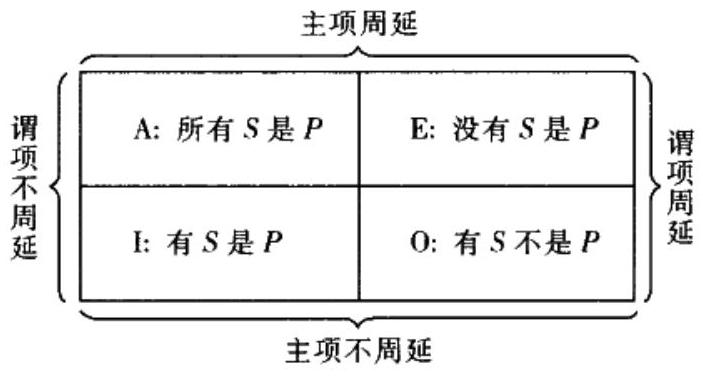
\includegraphics[max width=\textwidth, center]{2025_05_15_6a28331d5e7c993ad07ag-234}

\section*{练习题}
指出下列命题的质和量,并说明其主项和谓项的周延情况。\\
* 1 .有的总统候选人是让人们极度失望的人。\\
2.所有死于纳粹集中营的人都是残酷而无理性的专制制度的牺牲品。\\
3.某些新近确认的不稳定元素不是被偶然发现的。\\
4.有些军工联合体成员是无不良品行的善良人。\\
*5.没有女权主义运动的领导者是商业主管。\\
6.所有不惜任何代价维护法治强硬路线的人都是不了解 20 世纪后期巨大社会压力的人。

7.某些最高法院的新裁决是藐视整个美国法制史的决议。\\
8.没有有毒杀虫剂或化学落叶剂是对国家长远的农业发展目标有真正贡献的。

9.有些倡导政治、社会和经济大改革的人不是与维持现状利害相关的人。\\
*10.所有新的劳动集约型设备是工会运动的严重威胁。

\section*{5.4 传统对当方阵}
具有相同主项和相同谓项的标准式直言命题,可能在量上有所不同, 189 或者在质上有所不同,也可能在质与量上都不同。先前的逻辑学家称之为对当关系(opposition),各种对当关系之间有很重要的真值联系。

\section*{A.矛盾关系(Contradictories)}
两个命题之间具有矛盾关系,如果一个是另一个的拒斥(denial)或否定(negation),也就是说,它们既不能同真也不能同假。显而易见,如果两个标准的直言命题的主项相同、谓项也相同,而质、量都不同,那么,它们就是矛盾的。例如 A 和 O 就是这样的,比如:

所有法官都是律师。

与

有法官不是律师。

这两个命题的质与量都是对立的,显然它们是矛盾的。其中之一为真时,另一个恰恰为假。

同理, E 和 I 也是这样:

没有政客是理想主义者。

与

这两个命题的质与量都是对立的,因而它们是矛盾的。用公式表示就是: "所有 $S$ 是 $P$"的矛盾命题是"有 $S$ 不是 $P$",而"没有 $S$ 是 $P$"的矛盾命题是"有 S 是 P "; A 和 O 互为矛盾, E 和 I 互为矛盾。

\section*{B.反对关系(Contraries)}
两个命题之间具有反对关系,如果它们不能同时为真,也就是说,可以由一个的真推出另一个的假。例如,"得克萨斯队将在比赛中战胜俄克拉何马队"与"俄克拉何马队将在比赛中战胜得克萨斯队"就是反对的;如果两个命题中的一个(当然指的是在同一场比赛中)是真的,那么另一个必定为假。但它们不是矛盾的,因为如果他们打成平手,两个命题就同时为假。具有反对关系的两个命题,不能同时为真,但可以同时为假。传统逻辑或曰亚里士多德逻辑认为,如果两个直言命题都是全称的,其主、谓项分别相同而质不同,那么它们就是互相反对的。 ${ }^{[1]} \mathrm{A}$ 命题和相应的 E命题不能同时为真,却可以同时为假,所以它们之间是反对关系,例如 "所有诗人都是懒汉"与"没有诗人是濑汉"。

如果 A 命题或者 E 命题是必然真的一一即在逻辑上或数学上为真一一那么,说它们是互相反对的就是不正确的。例如,"所有三角形都是四边形"与"没有三角形是四边形"。如果一个命题是必然真的一一不可能为假的一一那么,它就没有反对命题,因为互相反对的命题可以同假。我们把既非必然真也非必然假的命题称为偶真的(contingent)。如果一个 A 命题和一个 E 命题都是偶真的,并且它们有相同的主项和相同的谓项,那么,说它们是反对的就是正确的。本章其他部分的讨论都假定 A和 E 是偶真的。

\section*{C.下反对关系(Subcontraries)}
两个命题之间具有下反对关系,如果它们不能同假,但可以同真。传统上认为,如果两个直言命题都是特称的,其主、谓项分别相同而质不同,那么它们之间是下反对关系。也就是肯定了 I 和 O 命题,可以同真但不可同假,如:

有钻石是珍贵的石头。

有钻石不是珍贵的石头。\\
必定是下反对的。\\
如果 I 和 O 必然为假,那么,说它们是下反对的就不正确。例如"有正方形是圆"与"有正方形不是圆"。如果一个命题必然为假——也就是说,不可能为真一一那么它就不会有下反对的对立面。因为,两个互为下反对的命题是可以同真的。当然,如果 I 和 O 都是偶真的,就可以同真。与反对关系一样,本章其他部分的讨论亦假定 I 和 O 都是偶真的。

\section*{D.差等关系(Subalternation)}
如果两个命题有相同的主项和相同的谓项,并且它们的质相同(即都是肯定的或者都是否定的),但量不同(即一个为全称,另一个为特称),那么,它们之间的关系就是差等关系。例如,A 命题:

\section*{所有蜘蛛都是八脚动物。}
有一个相应的 I 命题:

有蜘蛛是八脚动物。

191 而 E 命题:

\begin{displayquote}
没有鲸是鱼。
\end{displayquote}

也有一个相应的 O 命题:

\section*{有鲸不是鱼。}
此前用于说明命题间对当关系的例子都有"对立"(disagreement)的含义。但这里使用的"对当关系"是个专业术语,也适用于并不存在"对立"含义的情况。在上面的例子中,A 命题和相应的 I 命题之间不"对立",E命题和 O 命题之间也不"对立",但它们却都具有一种特殊的"对

当关系"。全称命题与相应的特称命题之间的对当关系叫做差等关系。在一对相应的命题中,比如刚才给出的两对,全称命题叫做"上位式",特称命题叫做"下位式"。

传统上认为,在差等关系中,上位的真蕴涵下位的真。举例来说,从全称肯定命题"所有鸟是有羽毛的"可以得出特称肯定命题"有鸟是有羽毛的";而从全称否定命题"没有鲸是鱼"可以得出特称否定命题"有鲸不是鱼"。但下位并不蕴涵上位。从特称肯定命题"有动物是猫"不能得出全称肯定命题"所有动物是猫"。同样,从特称否定命题"有动物不是猫"当然也不能推出"没有动物是猫"的结论。

\section*{E.对当方阵}
命题之间这四种对当关系——矛盾关系、反对关系、下反对关系以及上位与下位之间的差等关系——可以用一个重要且广为应用的图示来表示,称为"对当方阵",见图 5-1。\\
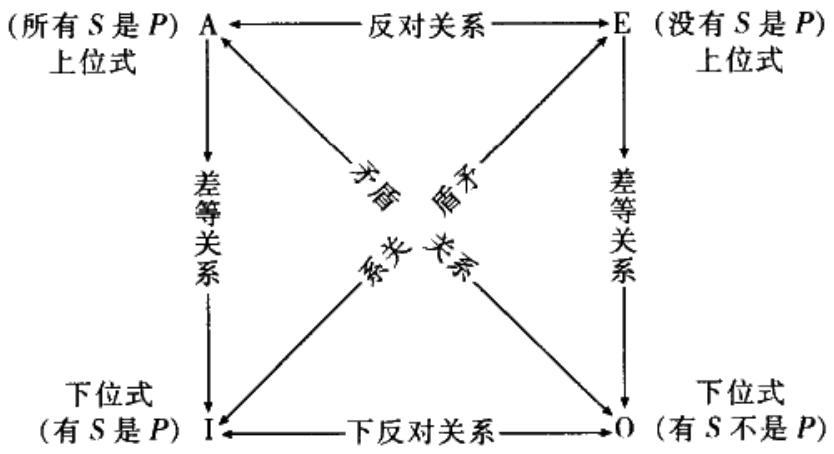
\includegraphics[max width=\textwidth, center]{2025_05_15_6a28331d5e7c993ad07ag-238}

图 5-1\\
展示在对当方阵中的关系,为把握论证的一些基本形式的有效性提供了一个逻辑基础。如果我们按照惯例将论证分为直接推论和间接推论,那就更容易理解了。

任何论证都是从一个或多个前提得出一个结论。包括一个以上前提的推论叫做间接推论,例如三段论,其结论就是从第一个前提经由第二个前提为中介得出的。而如果从唯一的前提出发,不经过任何中介推得结论,这样的推论叫做直接推论。容易见得,许多非常有用的直接推论,可从传统对当方阵所包含的知识中获得。

下面看一些例子。如果以 A 命题为前提,根据对当方阵,可以有效

地推出相应的(即主、谓项分别相同的)O命题为假。从同样的前提也可以有效地推出相应的 I 命题为真。当然,从 I 命题的真不能推出相应的 A命题为真,但可以推出其矛盾命题 E 为假。以对当方阵为基础,还可以得到许多这样的直接推论。给定任一标准式直言命题的真假情况,就可以直接得到其他某个或者所有其他相应命题的真假情况。基于对当方阵的直接推论可以列表如下:

如果 A 真,那么, E 假、 I 真、 O 假;\\
如果 E 真,那么, A 假、 I 假、O 真;\\
如果 I 真,那么,E 假,A、O 真假不定;\\
如果( )真,那么,A 假,E、I 真假不定;\\
如果 A 假,那么,O 真,E、I 真假不定;\\
如果 F 假,那么, I 真, A 、O 真假不定;\\
如果 I 假,那么, A 假、 E 真、O 真;\\
如果 O 假,那么, A 真、 E 假、 I 真。 ${ }^{[2]}$

\section*{练习题}
在给定的假定下,推论各组中其他命题的真假情况。\\
(1)假定第一个命题为真;(2)假定第二个命题为假。\\
*1.a.所有事业有成的经理是有头脑的人。\\
b.没有事业有成的经理是有头脑的人。\\
c.有的事业有成的经理是有头脑的人。\\
d.有的事业有成的经理不是有头脑的人。\\
2.a.没有有角动物是肉食动物。\\
b.所有有角动物是肉食动物。\\
c.有有角动物是肉食动物。\\
d.有有角动物不是肉食动物。\\
3.a.有的铀同位素是极不稳定的物质。\\
b.有的铀同位素不是极不稳定的物质。\\
c.所有铀同位素是极不稳定的物质。\\
d.没有铀同位素是极不稳定的物质。

4.a.有些大学教授不是风趣的演讲者。\\
b.所有大学教授是风趣的演讲者。\\
c.没有大学教授是风趣的演讲者。\\
d.有些大学教授是风趣的演讲者。

\section*{5.5 其他直接推论}
除了基于对当关系的直接推论,还有另外一些直接推论,本节我们来讨论其中的三种。

\section*{A.换位法(Conversion)}
第一种叫做换位法,它是一种仅仅通过交换命题中主、谓项的位置而进行的推论。对于 E 命题和 I 命题来说,换位法肯定是有效的。很显然,若断言"没有人是天使",也就可以断言"没有天使是人"。这两个命题可以通过换位法进行有效的互推。同样显然的是,"有作家是妇女"与"有妇女是作家"在逻辑上也是等价的,可以通过换位从其中一个有效地推出另一个。一个标准式直言命题叫做另一个的换位命题,如果它是通过交换另一个命题的主、谓项的位置而得到的。例如,"没有理想主义者是政治家"是"没有政治家是理想主义者"的换位命题,它们可以通过换位有效地互推。换位法直接推论中的前提叫做被换位命题(convertend),结论叫做换位命题(converse)。

请注意,从被换位 A 命题不能普通有效地推出换位 A 命题。比如,已知"所有狗是动物",当然不能有效地推出它的换位命题"所有动物是狗",因为被换位命题为真,而换位命题为假。传统逻辑自然也认识到这一点,但它认为对于 A 命题进行某种类似换位的推论可以是有效的。如 5.4 节表明,依据对当方阵,从 A 命题(所有 $S$ 是 $P$ )可以有效地推出其相应的下位 I命题(有 $S$ 是 $P$ )。A 命题说的是 $S$ 类中全部元素的情况,而 I 命题则限制为只述及 $S$ 类中的部分元素的情况。我们已经知道 I 命题是可以有效换位的。

这样,给定一个 A 命题(所有 $S$ 是 $P$ ),就可以根据差等关系,有效地得到相应的下位命题(有 $S$ 是 $P$ ),而下位命题(有 $S$ 是 $P$ )又可以进行有效换位,因此,通过差等关系和换位法的结合,从所有 $\boldsymbol{S}$ 都是 $\boldsymbol{P}$ 就可有效地推出有 $\boldsymbol{P}$ 是 $\boldsymbol{S}$ 。这种推论称为限制换位(或"偶然换位"[conver-\\
sion per accidens]),即交换主谓项的位置,同时将命题的量由全称改为特称。因此,按照传统逻辑的认识,"所有狗都是动物"可以有效地推出"有动物是狗",这个推论就是"限制换位"。下一节将进一步探讨这个问题。

请注意,作为限制换位结论的换位命题与原来的 A 命题并不等价,原因在于限制换位需要改变命题的量,把全称改为特称。因此,限制换位的结果不是一个 A 命题而是 I 命题,它不可能与被换位命题有同样的意义,从而不可能在逻辑上等价。但 E 命题的换位命题仍是一个 E 命题, I命题的换位命题仍是一个 I 命题,在这样的情况下,被换位命题与换位命题有同样的量,并且在逻辑上是等价的。

最后需要注意的是, O 命题的换位一般是无效的。 O 命题"有动物不是狗"很明显是真的,但它的换位命题"有狗不是动物"显然是假的。O命题与其换位命题并不等价。

一命题的换位命题总与原命题词项相同(只是位置互换),并且质也相同。下表是对传统换位推论的完整描述:

\section*{B.换质法(Obversion)}
接下来讨论的直接推论类型叫做换质法。在解说之前,我们先简要回顾一下"类"这个概念,并由此引人一些新的概念,以便更容易讨论换质法。一个类就是具有某种共同属性的所有对象的汇集。这种共同属性叫做 "类的定义特征"(class-defining characteristic)。举例来说,所有人的类就是所有具有"是人"这个特征的事物的集合,属性"是人"就是这个类的定义特征。类的定义特征不一定是"简单"的属性,任何一个属性都可以确定一个类。比如"左撒子、有红头发并且是学生"这个复杂属性就确定了一个类——所有是左撇子、有红头发的学生的类。

所有的类都有一个相应的补类(complementary class),或简称补 (complement),即不属于原来的类的所有东西的汇集。比如,所有人的类

的补就是所有不是人的东西组成的类。该类的定义特征是不是人这样一个 (否定的)属性。所有人的类的补包括除人之外的所有东西:鞋子、轮船、封蜡和大白菜等等——但不包括国王,因为国王是人。把所有人的类的补称为"非人的类"更简洁一些,词项 $S$ 所指称的类的补则由词项非 $S$ 指称,因而可以说词项非 $S$ 就是词项 $S$ 的补。 ${ }^{[3]}$

我们在两种意义上使用"补"这个词:一是类意义上的补,二是词项的补。尽管两者有所不同,但却是密切联系着的。一个词项是另一词项的词项补,仅当第一个词项指称第二个词项所指称的类的补。应当说明的是,正如一个类是其(类)补的补一样,一个词项也是其(词项)补的补。其中用到了"双重否定"法则,这样就可以省去许多用做前缀的 "非"字。例如,如果把词项"选举人"的补写做"非选举人",而"非选举人"的补就简记为"选举人",而不是"非非选举人"。必须注意不要把反对词项当做互补词项,比如将"懦夫"等同于"非英雄"。没有既是懦夫又是英雄的人,但并非每个人--当然更不是任何东西--都必须或者是懦夫或者是英雄,所以词项"懦夫"与"英雄"之间是反对关系。再比如 "胜者"的补不是"败者"而是"非胜者",因为并非所有东西——或者说所有人——必须或是胜者或是败者。但每个东西必定或是胜者或是非胜者。

了解了词项补的含义,换质法就比较容易描述了。在换质法中,主项保持不变,被换质命题的量也不需改变。对一个命题进行换质,就是改变其质,并用谓项的补替换原来的谓项。例如下面这个 A 命题:

所有居民都是选举人。

换质后成为一个 E 命题:

没有居民是非选举人。

泉然,这样两个命题在逻辑上是等价的,因此从一个可以有效地推出另一个。换质法应用到任何标准式直言命题,都是有效的直接推论。例如,下面的 E 命题:

换质后得到一个等值的 A 命题:

所有仲裁人都是不偏心的。

同样的,I 命题:

有金属是导体。

换质后得到一个 O 命题:

有金属不是非导体。

最后,()命题:

有国家不是好战的。

换质后得到一个 I 命题:

有国家是不好战的。

换质法直接推论中的前提叫做被换质命题(obvertend),结论叫做换质命题(obverse)。所有标准式直言命题与其换质命题在逻辑上都是等价的,所以,对任何一个标准式直言命题而言,换质法都是有效的。要得到一个命题的换质命题,不需改变原命题的量和主项,而是要改变它的质,并用谓项的补替换原来的谓项。下表对传统上的换质推理进行了全面的刻画:

\begin{center}
\begin{tabular}{|l|l|}
\hline
\multicolumn{2}{|c|}{换质表} \\
\hline
被换质命题 & 换质命题 \\
\hline
A:所有 $S$ 是 $P$ & E :没有 $S$ 是非 $P$ \\
\hline
E :没有 S 是 $P$ & A:所有 $S$ 是非 $P$ \\
\hline
I:有 $S$ 是 $P$ & O :有 $S$ 不是非 $P$ \\
\hline
O :有 $S$ 不是 $P$ & I :有 $S$ 是非 $P$ \\
\hline
\end{tabular}
\end{center}

\section*{C.换质位法(Contraposition)}
讨论第三种直接推论并不需要引人新的原理,从一定意义上讲,这种方法可以还原为前面两种推论。对给定的命题进行换质位,就是将主项换为原命题谓项的补,并将其谓项换为原命题主项的补。例如,A命题:

所有会员都是选举人。

换质位后是 A 命题:

所有非选举人都是非会员。

容易见得,以上两个命题在逻辑上是等价的。对 A 命题进行换质位是有效的直接推论形式。对 A 命题首先换质,再换位,然后再换质,于是就从最初的"所有 $S$ 是 $P$"转化为"所有非 $P$ 是非 $S$"。因此,对任何一个 A 命题进行换质位,都是将原命题先换质,再换位,然后再换质。

换质位法用于 A 命题是最有用的,用于 O 命题也是有效的直接推论形式。例如对于 $O$ 命题:

有学生不是理想主义者。

换质位后得到一个有点绕口的 O 命题:

有非理想主义者不是非学生。

它与第一个命题在逻辑上是等价的。如果每次只转化一步,即先换质,再换位,再换质,那么就可以显示出其逻辑等价性。可把其中的推论用公式表示为:从"有 $S$ 不是 $P$"换质得"有 $S$ 是非 $P$",再换位得"有非 $P$ 是 $S$",继续换质得"有非 $P$ 不是非 $S$"(换质位命题)。

一般说来,换质位法对于 I 命题无效。用下面这个真的 I 命题可以证明这一点:

有公民是非议员。

换质位后得到一个假命题:

有议员是非公民。

其无效的原因在于对 I 命题进行换质位,就要对 I 命题先换质,再换位,然后再换质。I命题"有 $S$ 是 $P$"换质后得 O 命题"有 $S$ 不是非 $P$",而后者一般不能有效换位。

E 命题"没有 $S$ 是 $P$"的换质位命题是"没有非 $P$ 是非 $S$",这也不是从原命题有效地得出的,下面的例子可以说明这一点, E 命题:

没有摔跤运动员是体弱的人。

其为真,但完全换质位命题却是假的:

没有非体弱的人是非挥跤运动员。

为了得到其换质位命题,我们对 E 命题先进行换质,再换位,然后再换质,就可以找到无效的原因。 E 命题"没有 $S$ 是 $P$"换质后得 A 命题 "所有 $S$ 是非 $P$"。一般说来,A命题不能有效地换位,除非进行限制换位。于是,通过限制换位得"有非 $P$ 是 $S$",再换质得"有非 $P$ 不是非 $S$",我们称之为"限制换质位"。下一节我们将进一步讨论这个问题。

请注意,通过限制性换质位法,我们可从一个 E 命题推得一个 O 命题——一即从"没有 $S$ 是 $P$"推出"有非 $P$ 不是非 $S$"——与限制换位有同样的特点。由于从全称命题只能推特称命题,结果得到的换质位命题与原命题意义不同,与作为原命题的 E 命题逻辑上不等价。而 A 命题的换质位命题仍是 A 命题, O 命题的换质位命题仍是 O 命题,在这两种情况下,换质位命题与其前提是等值的。

因此,换质位法只对 A 命题和 O 命题是有效的,对 I 命题是无效的,对 E 命题进行限制换质位才是有效的。也可以用一个图表来完整刻画这种

\begin{center}
\begin{tabular}{|l|l|}
\hline
\multicolumn{2}{|c|}{换质位表} \\
\hline
前提 & 完全换质位命题 \\
\hline
A:所有 $S$ 是 $P$ & A:所有非 $P$ 是非 $S$ \\
\hline
E :没有 $S$ 是 $P$ & O :有非 $P$ 不是非 $S$(限制) \\
\hline
I:有 $S$ 是 $P$ & (换质位无效) \\
\hline
O :有 $S$ 不是 $P$ & O :有非 $P$ 不是非 $S$ \\
\hline
\end{tabular}
\end{center}

还有一些其他类型的直接推论,也都有各自的分类与特定名称,但并不需要引人新原理,我们在此就不再讨论了。

若要解决关于命题之间关系的某些问题,最好的方法就是研究从其中一个可以推得另一个的各种直接推论。例如,假定命题"所有外科医生都是内科医生"为真,是否可以推知"没有非外科医生是非内科医生"的真假情况?在此可以给出一个有用的方法,就是尽可能从给定命题推出多个有效结论,来看要考察的命题——或其矛盾命题和反对命题——是否能从为真的原命题有效地推出。上面的例子中,已知"所有 $S$ 是 $P$",我们可以有效地推出其换质位命题"所有非 $P$ 是非 $S$",再限制换位得"有非 $S$是非 $P$"——按照传统逻辑,它是已知命题的有效结论,因此是真的。根据逻辑方阵,它与被考察的命题"没有非 $S$ 是非 $P$"为矛盾关系,因此被考察的命题就是假的。

如 1.9 节所指出的,一个有效推理,如果前提为真,其结论必然为真。但如果前提为假,结论却可能为真。我们立即会联想到限制换位、限制换质位以及差等关系推理,它们正是后面一种情况的例子。例如,从假前提"所有动物是猫",根据差等关系推理,可以推出"有动物是猫"这样一个真结论。而假前提"所有父母都是学者"限制换位后也可以得到一个真结论"有学者是父母"。因此,如果已知一个命题为假,那么另一个(与之多少有些关系的)命题的真假情况就成了问题。比较好的方法是,从已知命题的矛盾命题或被考察命题本身着手。因为一个假命题的矛盾命题必然为真,所有从后者开始的有效推理也必然是真命题。而如果从被考察命题能够推出已知为假的命题,那么它本身也必然是假的。

\begin{center}
\begin{tabular}{|l|l|}
\hline
\multicolumn{2}{|c|}{换位法、换质法、完全换质位法} \\
\hline
\multicolumn{2}{|c|}{换位法} \\
\hline
被换位命题 & 换位命题 \\
\hline
A:所有 $S$ 是 $P$ & I:有 $P$ 是 $S$ \\
\hline
E :没有 S 是 $P$ & E :没有 $P$ 是 $S$ \\
\hline
I:有 $S$ 是 $P$ & I:有 $P$ 是 $S$ \\
\hline
O :有 $S$ 不是 $P$ & (换位无效) \\
\hline
\multicolumn{2}{|c|}{换质法} \\
\hline
被换质命题 & 换质命题 \\
\hline
A:所有 $S$ 是 $P$ & E :没有 $S$ 是非 $P$ \\
\hline
E :没有 $S$ 是 $P$ & A:所有 $S$ 是非 $P$ \\
\hline
I:有 $S$ 是 $P$ & O:有 $S$ 不是非 $P$ \\
\hline
O :有 $S$ 不是 $P$ & I:有 $S$ 是非 $P$ \\
\hline
\multicolumn{2}{|c|}{换质位法} \\
\hline
前提 & 完全换质位命题 \\
\hline
A:所有 $S$ 是 $P$ & A:所有非 $P$ 是非 $S$ \\
\hline
E :没有 $S$ 是 $P$ & O :有非 $P$ 不是非 $S$(限制) \\
\hline
I:有 $S$ 是 $P$ & (换质位无效) \\
\hline
O :有 $S$ 不是 $P$ & O :有非 $P$ 不是非 $S$ \\
\hline
\end{tabular}
\end{center}

\section*{练习题}
I.给出下列命题的换位命题,并指出哪些与被换位命题等价。\\
*1.没有关心别人的人是不顾交通法规的鲁葬驾车人。\\
2.所有西点军校的毕业生是美国军队任命的军官。\\
3.有些欧洲轿车是价高质差的汽车。\\
4.没有爬行动物是恒温动物。\\
*5.有专业摔跤运动员是体力不支的老者。\\
II.给出下列命题的换质命题。\\
*1.有大学选手是职业运动员。\\
2.没有有机化合物是金属。\\
3.有牧师不是戒酒的人。

4.没有天才是墨守成规者。\\
-5.所有适于作锚的东西是至少重十五磅的东西。\\
III.给出下列命题的换质位命题,并指出哪些与原命题等价。\\
*1.所有记者是悲观主义者。\\
2.有士兵不是军官。\\
3.所有学者是不堕落者(nondegenerates)。\\
4.所有轻于五十磅的东西是不高于四英尺的东西。\\
*5.有非公民不是非居民。\\
N.如果命题"所有社会主义者是和平主义者"为真,那么下列命题的真假情况如何?或者说,请指出下列哪些命题是真的,哪些命题是假的,哪些是真假不定的?\\
*1.有非和平主义者不是非社会主义者。\\
2.没有社会主义者是非和平主义者。\\
3.所有非社会主义者是非和平主义者。\\
4.没有非和平主义者是社会主义者。\\
'5.没有非社会主义者是非和平主义者。\\
6.所有非和平主义者是非社会主义者。\\
7.没有和平主义者是非社会主义者。\\
8.有社会主义者不是和平主义者。\\
9.所有和平主义者是社会主义者。\\
*10.有非和平主义者是社会主义者。\\
V.如果命题"没有科学家是哲学家"为真,那么下列命题的真假情况如何?或者说,请指出下列哪些命题是真的,哪些命题是假的,哪些是真假不定的?\\
*1.没有非哲学家是科学家。\\
2.有非哲学家不是非科学家。\\
3.所有非科学家是非哲学家。\\
4.没有科学家是非哲学家。\\
*5.没有非科学家是非哲学家。\\
6.所有哲学家是科学家。\\
7.有非哲学家是科学家。\\
8.所有非哲学家是非科学家。

9.有科学家不是哲学家。\\
"10.没有哲学家是非科学家。\\
VI.如果命题"有圣徒是殉道者"为真,那么下列命题的真假情况如何?或者说,请指出下列哪些命题是真的,哪些命题是假的,哪些是真假不定的?\\
*1.所有圣徒是殉道者。\\
2.所有圣徒是非殉道者。\\
3.有殉道者是圣徒。\\
4.没有圣徒是殉道者。\\
*5.所有殉道者是非圣徒。\\
6.有非殉道者是圣徒。\\
7.有圣徒不是非殉道者。\\
8.没有殉道者是圣徒。\\
9.有非圣徒是殉道者。\\
*10.有殉道者曾是非圣徒。\\
11.有圣徒不曾是殉道者。\\
12.有殉道者不曾是圣徒。\\
13.没有圣徒曾是非殉道者。\\
14.没有非圣徒曾是殉道者。\\
*15.有殉道者不曾是非圣徒。\\
VII.如果命题"有商人不是海盗"为真,那么下列命题的真假情况如何?或者说,请指出下列哪些命题是真的,哪些命题是假的,哪些是真假不定的?\\
*1.没有海盗是商人。\\
2.没有商人是非海盗。\\
3.有商人是非海盗。\\
4.所有非商人是海盗。\\
*5.有非商人是非海盗。\\
6.所有商人是海盗。\\
7.没有非商人是海盗。\\
8.没有海盗是非商人。\\
9.所有非海盗是非商人。\\
'10.有非海盗不是非商人。\\
11.有非海盗是商人。\\
12.没有非海盗是商人。\\
13.有海盗是商人。\\
14.没有商人是非海盗。\\
*15.没有商人是海盗。

\section*{5.6 存在含义与直言命题的解释}
进一步分析和评估由直言命题构成的论证,需要对它们进行图示与符号化。但是,把 A、E、I、O 命题符号化,必定会遇到而且必须解决一个深层的逻辑问题——一个上千年长期争论的问题。本节我们就来说明这个问题,同时提供一种解决方案。以此为基础,也可以对三段论做出融贯的分析。

首先要说明的是,这并不是一个简单的问题。但只要我们弄清如下关于直言命题的解释(称为布尔解释[Boolean interpretation]),则后面关于三段论的分析并不需要对有关争议的深度把握。如果能掌握本节最后所总结的讨论结果,就可以顺利越过此前的复杂讨论。

要理解这个结果,必须弄清有些命题有存在含义(existential im- port),有些则没有。如果说出一个命题就肯定了某种对象的存在,那么就说这个命题有存在含义。

为什么初学逻辑就要关心这个看上去很深奥的问题呢?这是因为,特定论证中所用的命题中是否有存在含义,将直接影响到该论证中推理的正确性。对直言命题必须有一个清晰、融贯的解释,以便能确定什么东西可以从它们正确地推出,同时避免错误推论。

先看 I 命题和 O 命题,它们肯定有存在含义。例如 I 命题"有士兵是英雄"说的是至少存在一个是英雄的士兵。而 O 命题"有狗不是同伴"说的是至少存在一个不是同伴的狗。特称命题 I 和 O,一般说来,确实断定了主项(例句中的士兵和狗)指称的类不为空——士兵的类和狗的类(如果给出的例子为真的话)中至少有一个元素。 ${ }^{[4]}$

如果确实如此,即如果 I 和 O 命题有存在含义(没人会否认),会有

什么问题呢?问题在于这种状况的后果令人十分不安。先前我们已经说过,通过差等关系推论,I 命题可以从相应的 A 命题有效地推出,也就是说,从"所有蜘蛛都是八脚动物"可以有效地推出"有蜘蛛是八脚动物"。同样,我们说 O 命题可以有效地从 E 命题推得。但如果 I 和 O 命题有存在含义,而它们分别是从 A 和 E 命题得到的,那么 A 和 E 命题必定也要有存在含义。因为一个有存在含义的命题不可能有效地从另一个没有同样含义的命题得到。 ${ }^{[5]}$

这种结果造成了一个严重的问题。我们知道在传统逻辑方阵中,A 和 O 命题是矛盾关系。"所有丹麦人都说英语"与"有丹麦人不说英语"是互为矛盾的。具有矛盾关系的命题不可同真,因为其中必有一假。两者也不可同假,因为其中必有一真。但如果像上文总结的那样,对应的 A 和 O命题确实有存在含义的话,那么,两个矛盾命题就可能同时为假!举例来说,A命题"所有火星人都是金发碧眼的"与其对应的 O 命题"有火星人不是金发碧眼的"互为矛盾,如果它们都有存在含义的话——即我们要把它们看做都断言存在火星人的话——那么,如果火星上没有居民则两个命题都是假的。我们当然知道火星上没有人,火星人的类是空类,据此上述例子中给出的两个命题都是假的。而如果两者都是假的,它们就不可能是矛盾关系!

由此看来,传统对当方阵是有不妥之处的。假如它所说 A 和 E 命题有效地蕴涵相应的 I 和 O 命题是正确的话,那么,它断言 A 和 O 命题之间有矛盾关系就不正确了,同样,认为 I 和 O 命题为下反对关系也是不正确的。

那么我们该怎么办呢?传统逻辑方阵还能否加以挽救?挽救是可以的,但代价很高。我们可以引入预设(presupposition)概念来恢复逻辑方阵的地位。我们早已注意到(见 4.3 节),对于一些复杂问语,只有已经预设了先行问题的答案,才能适当地回答"是"或"否"。只有预设了你偷过钱是真的,才能用"是"或"否"来回答"你把偷来的钱花光了吗"这样的问题,否则是不合理的。现在,为挽救传统逻辑方阵,我们可以主张所有直言命题,即四种标准式命题 A、E、I、O——都预设(在上述含义下)它们涉及的类均不为空,即都有元素。也就是说,要使命题的真假情况以及它们之间的逻辑关系都成立并可以得到合理的解答(在这种解释下),就必须预设它们绝不涉及空类。这样,就可以保留传统对当方

阵中构建的各种关系: A 与 E 仍是反对关系, I 与 O 仍是下反对关系, A与 $\mathrm{O} 、 \mathrm{E}$ 与 I 仍是矛盾关系。然而,为了保证这个结果,必须诉诸其全面存在预设(blanket presupposition),即预设全部词项指称的类(及其补类)都有元素,都不为空。 ${ }^{[6]}$

那么,我们为什么不能就此罢休呢?存在预设对于挽救亚里士多德型逻辑既是必要的也是充分的。而且,预设在很多情况下与现代语言的日常用法是一致的。如果有人告诉你说"桶里的苹果都是甜的",而你向桶里一看,却什么都没有,那你会怎么说?你可能不会说刚才的话是假的或真的,而是指出这里没有苹果。你会解释说,说话人犯了一个错误,即当时的存在预设(桶里有苹果)是假的。事实上,这种纠正已经表明我们理解并基本接受了日常语言中的预设。

然而不幸的是,用来挽救逻辑方阵的这种全面预设却要付出一个过重的代价,是我们不能接受的。我们有充分的理由不这样做,在此列举三条理由。

首先,引人预设确实能够保留 A、E、I 和 O 之间的对当关系,但却付出了不能刻画某些我们需要的断言的代价,即不能再刻画那些否定有元素存在的命题了。而这样的否定有时非常重要,是必须明确的。

其次,即使是日常语言的用法,也并不完全与全面存在预设一致,有时我们说的话并不假定所谈的类中有元素。例如,你说"所有非法侵入者都要被起诉",这句话根本不预设非法侵人者的类中已经有元素,相反,你这样说正是为了保证这个类维持空类。

再次,在科学界及其他理论界,我们通常希望进行没有任何存在预设的推理。例如牛顿第一运动定律断定的是不受任何外力作用的物体必然保持静止状态或匀速直线运动。这种定律可以是真的,而物理学家表述它并为它辩护的时候,并没有预设不受任何外力作用的物体存在。

这些问题的存在使得上述全面存在预设不能为现代逻辑学家所接受。我们应当放弃曾长期被认为是正确的亚里士多德型解释,而采用关于直言命题的现代解释。

直言命题的现代解释不再假定我们言说的类中必定有元素。拒绝这种假定的解释称为布尔解释。英国逻辑学家、数学家乔治•布尔(George Boole,1815-1864)是现代符号逻辑奠基人之一,这种新的解释就是以

他的名字命名的。 ${ }^{[7]}$\\
在本书以下部分,我们均采纳关于直言命题的布尔解释。现在我们就来阐明这种解释:

1.在某些方面,传统解释仍然成立。 $\mathbf{I}$ 和 $\mathbf{O}$ 命题在布尔解释中仍然有存在含义。所以,如果 $S$ 类为空,那么,命题"有 $S$ 是 $P$"为假,命题 "有 $S$ 不是 $P$"也为假。

2.全称命题 $\mathbf{A}$ 和 $\mathbf{E}$ 与特称命题 $\mathbf{O}$ 和 $\mathbf{I}$ 之间的矛盾关系也保持为真。也就是说,命题"所有人是会死的"与"有人不是会死的"互为矛盾,而命题"没有神灵是会死的"与"有神灵是会死的"亦互为矛盾。

3.在布尔解释中上述关系是完全融贯的,这是因为,全称命题被解释为没有存在含义。因此,即使 $S$ 类为空,命题"所有 $S$ 是 $P$"仍可以为真,"没有 $S$ 是 $P$"也可以为真。例如,即使独角兽不存在,"所有独角兽是有角的"与"没有独角兽是有翅膀的"都可以为真。而如果不存在独角兽,I 命题"有独角兽是有角的"就是假的,O 命题"有独角兽不是有翅膀的"同样为假。

4.在日常话语中,有时我们说出一个全称命题,确实假定了某事物的存在。当然,布尔解释也允许有这种表述,但要求用两个命题来表述,一个是有存在含义的特称命题,加之一个没有存在含义的全称命题。

5.采纳布尔解释会带来一些重要变化。相应的 $\mathbf{A 、 E}$ 命题可以同真,因此它们之间不再是反对关系。这似乎有点怪异,在后面 10.2 和 10.3 部分将给出详细的说明。现在弄清如下这点就足够了:在布尔解释中,"所有独角兽是有翅膀的"断言的是"如果有独角兽,那么,它是有翅膀的"。而"没有独角兽是有翅膀的"断定的是"如果有独角兽,那么,它是没有翅膀的"。如果确实不存在独角兽,这两个"如果……那么……"型的命题都可以为真。

6.类似的,在布尔解释中,因为 I 和 O 命题确实有存在含义。所以,如果主项指称的类为空,相应的 I 和 O 命题都是假的,因此相应的 I 和 O命题之间也不再是下反对关系。

7.在布尔解释中,差等关系——从 A 命题推出相应的 I 命题,从 E命题推出相应的 O 命题——不是普遍有效的。从一个没有存在含义的命题

当然不能得出一个有存在含义的命题。\\
8.布尔解释保留了一些直接推理: $\mathbf{E}$ 命题和 $\mathbf{I}$ 命题的换位推理, $\mathbf{A}$ 命题和 O 命题的换质位推理,所有命题的换质推理。但限制换位、限制换质位推理不再有效。

9.在布尔解释下,遌辑方阵转变为如下情形:方阵周边的关系不再成立,而对角线上的矛盾关系保持不变。

简言之,现代逻辑学家否定了全面存在预设。对于一个不能明确断定其中有元素的类,我们就不能假定它有元素,否则就是错的。任何依据这种错误假定的论证都会产生存在预设谬误,简称为存在谬误。现在有了清晰的布尔解释,我们就可以构造一个有力的体系,将标准式直言命题推理符号化、图示化。

\section*{练习题}
有些传统上认为有效的推论,在本书所采用的布尔解释下,却成了错误的,因为它们假定了某些类中有元素,所以犯了存在谬误。我们刚刚讨论了存在含义,它表明的正是这种错误的原因。下列每个论证中都犯有存在谬误,请指出其错误之处。

\section*{例题}
I.(1)没有数学家是拥有方的圆的人。\\
所以,(2)没有拥有方的圆的人是数学家。\\
所以,(3)所有拥有方的圆的人是非数学家。\\
所以,(4)有非数学家是拥有方的圆的人。

\section*{解答}
第(3)步到第(4)步无效。其中运用的是限制换位(也就是说,从所有 $S$ 都是 $P$ 推出有 $P$ 是 $S$ ),传统解释接受这种换位,但在布尔解释下是无效的。其基础是从一个全称命题推出一个特称命题,前面的讨论已经表明,全称命题并不肯定类中有元素,但特称命题却做了这种肯定。所以从(3)到(4)的过程中就暗中假定了(4)的谓项代表的类非空,或者说,假定了存在拥有方的圆的人!从(3)推出(4),犯了存在谬误。

II.(1)没有公民是能完成不可能的事的人。\\
所以,(2)没有能完成不可能的事的人是公民。\\
所以,(3)所有能完成不可能的事的人是非公民。\\
所以,(4)有能完成不可能的事的人是非公民。\\
所以,(5)有非公民是能完成不可能的事的人。\\
III.(1)没有小丑是能用拔靴带把自己提起来的人。\\
所以,(2)没有能用拔靴带把自己提起来的人是小丑。\\
所以,(3)有能用拔靴带把自己提起来的人不是小丑。(据此可得至少有一个能用拔靴带把自己提起来的人。)

N.(1)"没有独角兽是在布朗克斯(Bronx)动物园被发现的"为真。

所以,(2)"所有独角兽是在布朗克斯动物园被发现的"为假。\\
所以,(3)有独角兽不是在布朗克斯动物园被发现的。(据此可得至少存在一个独角兽。)

V.(1)"有美人鱼是大学女生联谊会的成员"为假。\\
所以,(2)"有美人鱼不是大学女生联谊会的成员"为真。(据此可得至少存在一个美人鱼。)

\section*{5.7 直言命题的符号系统与图解}
直言命题的布尔解释在很大程度上以空类概念为基础,为方便起见,可用一个特殊的符号来表示空类。此处我们用数字" 0 "来代表空类。说词项 $S$ 指称的类没有元素,就在 $S$ 和 0 之间划上等号。也就是说,$S=0$表示 $S$ 没有元素( $S$ 的元素 $s$ 简记为 $S^{\prime} s$ ,说不存在 $S^{\prime} s$ 亦即 $S=0$ )。

说 $S$ 指称的类确实有元素就是否定 $S$ 为空。断定"存在 $S$'$s$"就是对 $S=0$ 所表示的命题的否定。我们在等号上加一条斜线表示这种否定式。就是说,$S \neq 0$ 表示存在 $S$'s,是对 $S$ 为空的否定。

标准式命题都涉及两个类,所以表示它们的等式要复杂一些。两个类都分别由一个符号代表,因此可以把两个符号并排在一起,用以表示那些由同时属于两个类的元素组成的类。比如,如果 $S$ 代表所有"讽刺作品"组成的类,$P$ 代表所有"诗"组成的类,那么,既是讽刺作品又是诗的东西组成的类就可以用符号 $S P$ 表示,它代表的就是所有讽刺诗(或者说诗

式讽刺作品)组成的类。两个类的共同部分或全体共同元素称为两个类的积(product)或交(intersection)。两个类的积是所有同时属于这两个类的东西组成的类。所有美国人的类与所有作家的类之积就是所有美国作家的类。(此处必须与自然语言的某些特定用法区分开来。例如,西班牙人的类与舞蹈家的类之积,不是西班牙舞蹈家的类,因为通常说的西班牙舞蹈家不是西班牙的舞蹈家,而是表演西班牙舞蹈的人。同样,抽象画家、英语课程、古董商人等等也都是这样的用法。)

使用这种新记法,我们也可以用等式和不等式将 E 和 I 命题符号化。 E 命题"没有 $S$ 是 $P$"说的是 $S$ 类中没有元素是 $P$ 类的元素,即没有东西同时属于两者。换言之,两个类的积为空,可用等式符号表示为: $S P=0$ 。I命题"有 $S$ 是 $P$"说的是 $S$ 类中至少有一个元素也是 $P$ 类的元素。这意味着 $S$ 类和 $P$ 类的积不空,可用不等式符号表示为: $S P \neq 0$ 。

对于 A 命题和 O 命题,需要引人一个表示补类的新方法。如 5.5 节所说明,一个类的补类就是所有那些不属于原类的东西的类或汇集。例如,士兵的类的补类就是所有不是士兵的东西组成的类,即非士兵的类。若用 $S$ 代表士兵的类,则把非士兵的类记为: $\bar{S}$(读做:$S$ 杠),即在原来的类之上加一横杠。A 命题"所有 $S$ 是 $P$"说的是 $S$ 类的所有元素都是 $P$类的元素,也就是说,没有 $S$ 类的元素不是 $P$ 类的元素。或者说(据换质法)"没有 $S$ 是非 $P$",像任何 E 命题一样,这个命题说的是,主项指称的类与谓项指称的类的积为空,可用等式符号表示为:$S \bar{P}=0$ 。 O 命题 "有 $S$ 不是 $P$"换质后得逻辑等价式 I 命题"有 $S$ 是非 $P$",可用等式符号表示为:$S \bar{P} \neq 0$ 。

使用这些符号公式,就能很清晰地显示四种标准式直言命题之间的相互关系。既然 A 命题和 O 命题的符号公式分别为 $S \bar{P}=0$ 和 $S \bar{P} \neq 0$(1),它们显然是互为矛盾的。E命题和I命题的符号形式分别为:$S P=0$ 和 $S P \neq$ 0 ,显然也是互为矛盾的。布尔解释下的对当方阵可以重新表示为图5-2。

命题可以用所涉及的类的图示来表达。我们用一个圆代表一个类,用 210指称类的词项标注它。这样 $S$ 类可以表示为图 5-3。

\footnotetext{(1)原书错印为 $\mathrm{SP} \neq 0$ 。
}
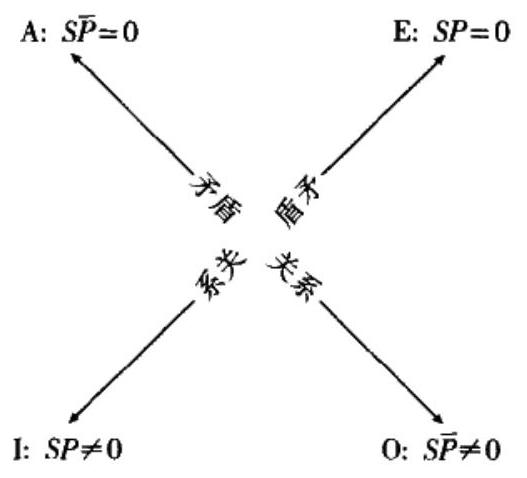
\includegraphics[max width=\textwidth, center]{2025_05_15_6a28331d5e7c993ad07ag-257(2)}

图5-2\\
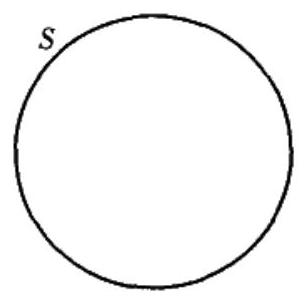
\includegraphics[max width=\textwidth, center]{2025_05_15_6a28331d5e7c993ad07ag-257}

图5—3\\
上图表示的是一个类,而不是命题。它只代表 $S$ 类,而对这个类无所言说。要图示命题"$S$ 没有元素"或"不存在 $S$'s",我们就在代表 $S$ 的圆中加上阴影,来表示 $S$ 中什么都没有,$S$ 为空类。要图示"存在 $S$'$s$"这个命题,我们就在代表 $S$ 的圆中写一个 $x$ ,用来表示其中有东西,$S$ 不是空类。这样,"不存在 $S$'s"和"存在 $S$'s"这两个命题就可以用图 5-4 来表示。\\
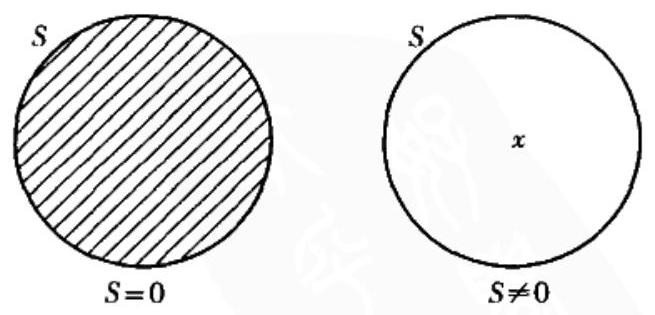
\includegraphics[max width=\textwidth, center]{2025_05_15_6a28331d5e7c993ad07ag-257(1)}

图 5-4\\
实际上,表示 $S$ 的图示也可以表示 $\vec{S}$ ,因为圆中的部分代表的是 $S$ 的所有元素,而圆外的部分恰好就是 $\bar{S}$ 。

要图示标准式直言命题,一个圆不够,而需要两个圆。标准式直言命题的主、谓项分别记为 $S$ 和 $P$ ,而后画两个相交的圆,如图 5-5。\\
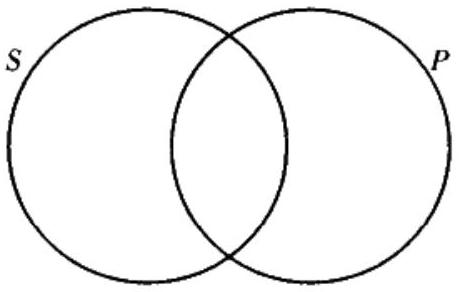
\includegraphics[max width=\textwidth, center]{2025_05_15_6a28331d5e7c993ad07ag-258}

图5-5\\
图示只表示出了 $S$ 和 $P$ 两个类,而没有表示它们形成的命题。既没有肯定也没有否定其中一个或两个类有元素。实际上,两个相交的圆表示出的类不只是 $S$ 和 $P$ 两个。标有 $S$ 的圆中与 $P$ 不重叠的部分代表的是所有不是 $P$'$s$ 的 $S$'$s$ ,即代表了 $S$ 类与 $\bar{P}$ 类的积,这一部分标记为 $S \bar{P}$ 。两圆相交的部分代表 $S$ 类与 $P$ 类的积,标记为 $S P$ 。标有 $P$ 的圆中与 $S$ 不重叠的部分代表的是所有不是 $S$'$s$ 的 $P$'$s$ ,即代表了 $\bar{S}$ 类与 $P$ 类的积,标记为 $\bar{S} P^{\oplus}$ 。最后,两个圆之外的部分,代表既不在 $S$ 类也不在 $P$ 类之中的东西,标记为第四个类 $\overline{S P}$ 。加上这些标记,图5-5就成了图5-6:\\
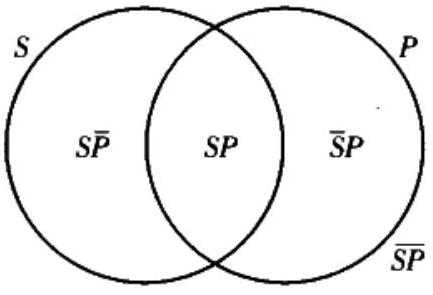
\includegraphics[max width=\textwidth, center]{2025_05_15_6a28331d5e7c993ad07ag-258(1)}

图 5-6\\
可以用各种不同的类来解释上图。例如设西班牙人的类为 $S$ 、画家的类为 $P$ ,则 $S P$ 就是两个类的积,由所有同时属于两个类的东西组成。因为 $S P$ 的每个元素必须既是 $S$ 类也是 $P$ 类的元素,所以每个元素既是西班牙人又是画家。两个类的积就是西班牙画家的类,其中包括委拉斯开兹 (Velásquez)和戈雅(Goya)等人。S $\bar{P}$ 是第一个类与第二个类之补的积,包括且只包括属于 $S$ 类但不属于 $P$ 类的对象,也就是不是画家的西班牙

人组成的类,即所有非画家西班牙人,委拉斯开兹不在其中,戈雅也不在其中,但却包括小说家塞万提斯(Cervantes)和独裁者佛朗哥(Franco)及其他西班牙人。 $\bar{S} P$ 是第二个类与第一个类之补的积,是那些不是西班牙人的画家组成的类,这个类包括荷兰画家伦布兰特(Rembrandt)、美国画家乔治亚•奥基夫(Georgia O’Keeffe)等。最后,$\overline{S P}$ 是原来两个类的补的积,包括而且只包括那些既不是西班牙人也不是画家的对象。这可是一个很大的类,包括的不只是英国海军上将和瑞士登山运动员们,还包括诸如密西西比河、珠穆朗玛峰这样的东西。如果对 $S$ 和 $P$ 进行这样的解释,那么,以上说的所有类都在图 5-6 中有所表示。

这就是文恩图(Venn diagram),得名于英国数学家、逻辑学家约翰•文恩(John Venn,1834-1923),他首先使用这种方法表示类和命题。像图 5-6 这样的带有几处标记的双圆图,所代表的仍只是类,尚不表示任何命题。整个圆或其中留做空白的部分既不表示类中有元素,也不表示没有。

但是,再加上一定条件,我们就能用文恩图来表示命题。通过给某些部分加上阴影,或者标上"$x$",就能准确地将四种标准式直言命题图示化。文恩图(带有标记的)能够全面、简明地表示命题,所以,它已经被公认为评价三段论论证的最有力、使用最广泛的方法。下面就来说明如何用文恩图表示这四种标准式命题。

A 命题"所有 $S$ 是 $P$"即 $S \bar{P}=0$ ,用文恩图图示之,可把代表 $S \bar{P}$ 的那部分加上阴影,即表示其中没有元素。 E 命题"没有 $S$ 是 $P$"即 $S P=0$ ,可把图中代表 $S P$ 的那部分加上阴影,以示其中没有元素。1 命题"有 $S$是 $P$"即 $S P \neq 0$ ,可在图中 $S P$ 类部分标上一个 $x$ ,表示两个类的积不是空的,其中至少有一个元素。最后, O 命题"有 $S$ 不是 $P$"即 $S \bar{P} \neq 0$ ,可加一个 $x$ 在 $S \bar{P}$ 部分,表示其中至少有一个元素而不是空的。将以上四个图示列在一起,就能十分清晰地展现出四种命题的不同含义,见下图 5-7。

我们已经用文恩图表示出"没有 $S$ 是 $P$"和"有 $S$ 是 $P$",而它们换位后分别得到一个等价命题:"没有 $P$ 是 $S$"和"有 $P$ 是 $S$",因此后面两个命题在图中也就表示出来了。要图示 A 命题"所有 $P$ 是 $S$"即 $P \bar{S}=0$ ,循同样路径,可把代表 $P \bar{S}$ 的部分加上阴影。显然,$P \bar{S}$ 与 $\bar{S} P$ 是相同的,如果一下子不能明白,就回想一下是画家而非西班牙人的类,与非西班牙人中是画家的类。前一个类中的对象必定也是后一个类的对象——即所有

是画家而非西班牙人的人与所有非西班牙人的画家,反之亦然。要图示命题"有 $P$ 不是 $S$"即 $P \bar{S} \neq 0$ ,可在 $P \bar{S}(=\bar{S} P)$ 部分加上一个 $x$ 。图 5--8展示的正是这几个命题。\\
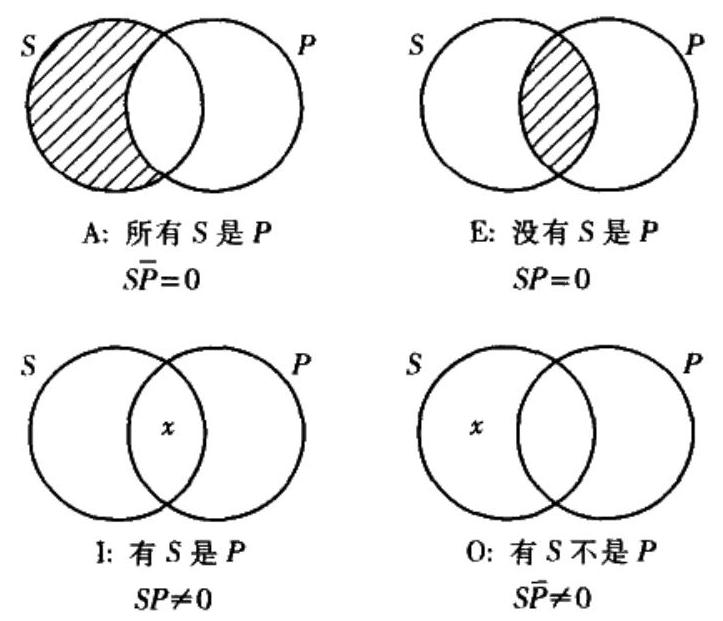
\includegraphics[max width=\textwidth, center]{2025_05_15_6a28331d5e7c993ad07ag-260(1)}

图5-7\\
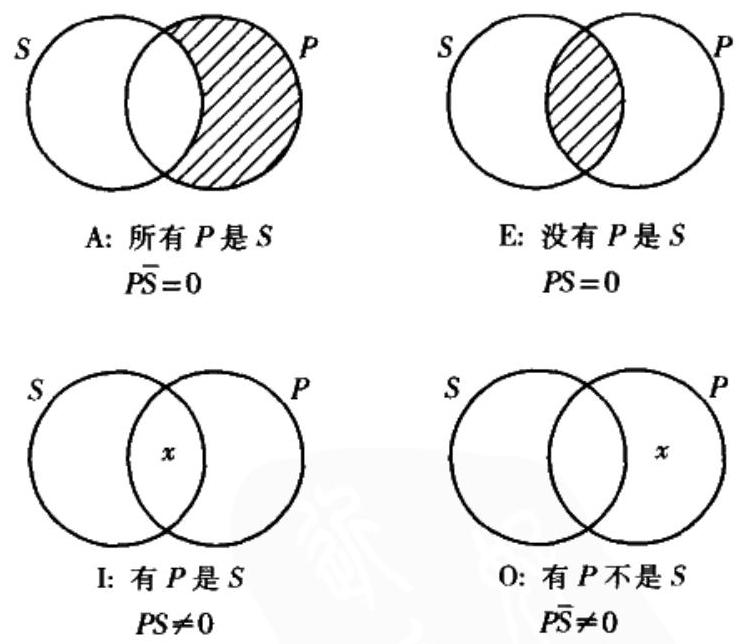
\includegraphics[max width=\textwidth, center]{2025_05_15_6a28331d5e7c993ad07ag-260}

图 5-8\\
双圆图的这种灵活运用,在本书下一章中起着重要作用。任给一对带有给定标记——比如 $S$ 和 $M$ ——的交叉圆,就能将任何一个含有 $S$ 和 $M$的标准式直言命题图示化,无论 $S$ 和 $M$ 出现的顺序如何。

文恩图是标准式直言命题的肖像,将空间的包含与排斥与类间非空间

的包含与排斥对应起来,是一种极为清晰的记法。下一章将会看到,这也是检验直言三段论的有效性的一种最简单、最直接的方法。

\section*{练习题}
用主谓项的首拼字母 ${ }^{(1)}$ 代表相应的类,用等式或不等式表示下列各命题,并在文恩图中表示出来。

\section*{例题}
1.有雕刻家是画家。\\
解答:$S P \neq 0$\\
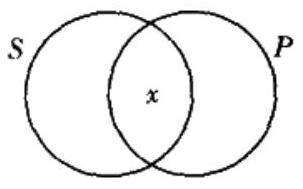
\includegraphics[max width=\textwidth, center]{2025_05_15_6a28331d5e7c993ad07ag-261}

2.没有小商贩是百万富翁。\\
3.所有商人是投机者。\\
4.有音乐家不是小提琴手。\\
5.没有商店老板是会员。\\
6.有名望很高的政治领导人是无赖。\\
7.所有拿到国家许可证的执业医生是通过了特定资格考试的医学院毕业生。

8.有提供投资建议的证券经纪人不是他们所推荐的公司的合伙人。\\
9.所有厌弃庸俗快乐的清教徒是极不习惯世俗生活方式的人。\\
*10.没有现代画作是跟照片一模一样的。\\
11.有学生积极分子是努力追回逝去岁月的中年人。\\
12.所有中世纪学者是修道院中虔诚的僧侣。\\
13.有国家公仆不是具有大众精神的人。\\
14.没有服从选举意见被召回的地方官是要受惩罚的专政者。\\
*15.有表现出所有精神分裂症状的病人是癫狂患者。\\
16.喷气式飞机上有乘客不是感到满意的消费者。

\footnotetext{(1)中译文读者可用汉语拼音首拼字母。
}17.有神职人员是积极鼓吹社会根本变革的人。\\
18.有现存秩序的忠实支持者不是政党成员。\\
19.没有穿越国界的输油管是安全设备。\\
*20.所有色情影片是文明和礼仪的大敌。

\section*{第5章概要}
本章介绍并讨论的是古典逻辑即亚里士多德型逻辑的基本构件,也是演绎逻辑的基本构件。\\
5.2 节介绍类的概念。传统逻辑正是以类为基础建立起来的。我们阐明了四种基本的标准式直言命题。

\begin{itemize}
  \item A 命题:全称肯定命题
  \item E 命题:全称否定命题
  \item I 命题:特称肯定命题
  \item O 命题:特称否定命题
\end{itemize}

5. 3 节更加详细地考察这四种命题。探讨了命题的质,即肯定和否定,以及命题的量,即全称和特称。说明了周延的项与不周延的项。\\
5.4 节探讨这几种直言命题之间的对当关系的种类:命题之间的矛盾关系、反对关系、下反对关系以及上位式与下位式之间的差等关系。并用一个对当方阵图示了这几种关系,进而说明了一些基于传统方阵的直接推理。\\
5.5 节阐明其他三种直接推论:换位法、换质法和换质位法。\\
5.6 节探讨存在含义问题。要保留传统对当方阵,只有做出一种假定,即全盘假定命题主项所指称的类总是有元素的一一这是现代逻辑极不赞同的。然后,我们又对本书通篇采用的布尔解释作了说明。布尔解释能保留传统逻辑对当方阵中的大部分内容,同时又避免了非空类的假定。在布尔解释中,特称命题,即称为 $\mathbf{I}$ 和 $\mathbf{O}$ 的命题之中有存在含义,但全称命题,即 $\mathbf{A}$ 和 $\mathbf{E}$ 则没有存在含义。我们也很细致地说明了采用这种解释的结果。\\
5.7 节介绍将直言命题符号化与图示化的方法,包括使用文恩图,用交叉的圆加以恰当的标记或阴影来刻画类与类之间的关系。

有了这些必要的工具,我们就可以考察——在接下来的两章中——建

基于标准式直言命题之上的三段论,以及传统演绎逻辑在日常语言中的其他主要用途。

\section*{【注释】}
[1] 5.6 节将对此传统观点作批判性讨论。\\
[2]纽约州立大学 Brockport 分校的约瑟夫•吉尔伯特(Joseph Gilbert)教授在其私人通信中提到,一个命题真假不定时,可能会产生一些意想不到的结论。如果已知 A 命题真假不定,我们可以推出其矛盾命题 O 必定也是真假不定的,因为如果知道 O命题为真或为假,那么 A 命题的真假也就能够确定了。对于 E命题及其矛盾命题也是这样。一般说来,如果一个命题是真假不定的,那么,它的矛盾命题必然也真假不定。如果 A 命题真假不定,其反对命题 E 必定为假,因为如果 E 为真,那么 A 就不是真假不定的。同理,如果已知 A 命题真假不定,那么相应的 I 命题必定为真。

如果已知 E 命题、 1 命题或者 O 命题真假不定,也可以运用类似的分析。结果就是:

如果 A 真假不定,那么,O 真假不定、E 假、I 真;\\
如果 E 真假不定,那么, I 真假不定、 A 假、 O 真;\\
如果 I 真假不定,那么, E 真假不定、 A 假、 O 真;\\
如果 O 真假不定,那么,A 真假不定、E 假、I 真。\\
[3]我们有时用类的"相对补"(relative complement)来进行推论,即它的补包含在另外一个类中。比如:"我的孩子"这个类有一个子类"我的女儿",后者的补是另一个子类"我的不是女儿的孩子",即"我的儿子"的类。但换质法以及其他直接推论通常建基于类的绝对补之上,正如上面所定义的那样。\\
[4]有极个别的例外情况,"有鬼出现在莎士比亚戏剧里"和"有希腊神在《伊利亚特》中有所描述"都是特称命题,它们当然是真的,虽然鬼和希腊神都不存在。但这是一种误导,因为这些描述本身并没有肯定或否定鬼和希腊神的存在,只是说某些特定的命题在莎士比亚的戏剧和《伊利亚特》中被肯定或否定。莎士比亚和荷马的命题不一定是真的,但他们的作品中肯定或暗含着这些命题。很明显,这只能说是例外情况,它们只出现在文学作品和神话语境中。I命题和 $O$ 命题确实是有存在含义的。\\
[5]有另外一种方法可以表明,传统逻辑方阵中 A 和 E 命题的存在含义必然是从 1 和 O 命题得到的。对于 A 命题,可以根据(传统逻辑中的)限制换位的有效性说明。对于 E 命题,可以根据(传统逻辑中的)限制换质位的有效性说明。得到的结果与上面是相同的:在传统選辑方阵中,如果 I 和 O 命题有存在含义,那么, A 和 E 命题必然也要有存在含义。\\
[6]韦伯(Phillip H.Wiebe)认为亚里士多德逻辑并不要求假定主项的补类非空。

见《亚里士多德逻辑中的存在预设》("Existential Assumptions for Aristotelian Logic", Journal of Philosophical Research 16 (1990-1991):321-328)。但亚里士多德逻辑确实要求假定:其他三个项(主项、谓项和谓项的补)所指称的类不是空的,而下面评论中的所有问题都是存在预设造成的。\\
[7]另一位现代符号逻辑奠基人伯特兰•罗素在著名的论文"The Existential Im- port of Propositions"(Mind,July 1905)中也阐发了这种解释。由于他是跟从 20 世纪初期的意大利伟大的数学家皮亚诺(Guiseppe Peano)学得这种解释,故称之为命题的"皮亚诺解释"。\\
6.1 标准式直言三段论\\
6.2 三段论论证的形式性质\\
6.3 检验三段论:文恩图解法\\
6.4 三段论规则和三段论谬误\\
6.5 直言三段论的 15 个有效形式\\
6.6 直言三段论 15 个有效形式的演绎推导

第6章概要

\section*{6. 1 标准式直言三段论}
三段论是从两个前提推得一个结论的演绎论证。直言三段论是由三个直言命题组成的演绎论证,其中包含且仅包含三个词项,每个词项在其构成命题中恰好出现两次。

如果一个直言三段论的前提、结论都是标准式的直言命题(A、E、 $\mathbf{1} 、 \mathbf{O})$ ,并且以特定的标准顺序组合在一起,就称为标准式直言三段论。要确定标准式直言三段论的顺序,必须首先说明直言三段论的词项和前提的特定名称,为简便起见,本章将直言三段论简称为"三段论"。其他三段论将会在后面的章节进行讨论。

\section*{A.大项、小项和中项}
标准式三段论的结论是一个标准式直言命题,三段论的三个词项有两个会在其中出现。因此,通过结论可以识别三段论的词项。

结论的谓项称为三段论的大项。\\
结论的主项称为三段论的小项。\\
在结论中不出现,而在前提中出现两次的项,即三段论的第三个项,称为中项。

例如下面这个标准式三段论中:

\begin{displayquote}
没有英雄是胆小鬼,\\
有士兵是胆小鬼,所以,有士兵不是英雄。
\end{displayquote}

"士兵"是小项,"英雄"是大项,结论中没有出现的"胆小鬼"是中项。\\
标准式三段论的前提因其中出现的项而得名。大项和小项必定出现在不同的前提中,包含大项的前提称为大前提,包含小项的前提称为小前提。在上述三段论中,大前提是"没有英雄是胆小鬼",小前提是"有士兵是胆小鬼"。

如前所述,如果前提以特定的标准顺序排列,就称这个三段论为标准式。现在即可描述这个顺序:在标准式三段论中,大前提处在第一位,小前提处在第二位,结论在最后。应当强调的是,大前提不是根据其位置而

确定的,而是因为其中包含大项,大项又是由结论的谓项定义的。同样的,小前提也不是根据其位置而确定的,而是因为其中包含小项,小项又是由结论的主项定义的。

\section*{B.式}
标准式三段论的式由所含直言命题的类型而定(以字母 $\mathbf{A 、 E 、 I 、 O}$为标志)。每个三段论的式都由三个按特定顺序排列的字母组成。第一个字母指的是大前提的类型,第二个字母指的是小前提的类型,第三个字母指的是结论的类型。例如,在上述作为例子的三段论中,大前提是一个 $\mathbf{E}$命题,小前提是一个 $\mathbf{I}$ 命题,结论是一个 $\mathbf{O}$ 命题,所以,这个三段论的式就是 EIO 式。

\section*{C.格}
只有式,还不能完全刻画标准三段论的形式。考虑下面两个三段论:\\
(A)所有大科学家都是大学毕业生,\\
有专业运动员是大学毕业生,\\
所以,有专业运动员是大科学家。

和\\
(B)所有艺术家都是自我主义者,\\
有艺术家是乞丐,\\
所以,有乞丐是自我主义者。

两个三段论的式都是 AII,但它们的形式并不相同。如果我们展示出它们的逻辑"骨架",就能十分清楚地揭示出其形式上的不同之处。把小项记为 $S$ ,大项记为 $P$ ,中项记为 $M$ ,并用"$\therefore$"表示"所以",这两个三段论的形式或"骨架"分别是:\\
(A)所有 $P$ 是 $M$ ,\\
有 $S$ 是 $M$ ,

\section*{(B)所有 $M$ 是 $P$ ,有 $M$ 是 $S$ ,}
\section*{$\therefore$ 有 $S$ 是 $P$ 。}
在记为(A)的第一个三段论中,中项在两个前提中都做谓项,而记为(B)的第二个三段论,中项在两个前提中都做主项。这两个例子表明,尽管三段论的形式可以部分地由式来描述,但相同式的三段论还是有区别的,这就要看中项的相对位置。 ${ }^{[1]}$ 然而,我们可以通过陈述一个三段论的格和式来完整地描述其形式,它的格表明了中项在前提中的位置。

显然,三段论有且只有四种不同的格。中项可能在大前提中做主项、在小前提中做谓项,或者在两个前提中都做谓项,或者在两个前提中都做主项,或者在大前提中做谓项、在小前提中做主项。中项的这些可能组合分别构成了三段论的第一、第二、第三和第四格。四个格的模式可依次排列如下,其中只显示了中项的相对位置,而隐藏了它们的式,也就是说既不出现量项也不出现联项:

$$
\begin{array}{llll}
M-P & P-M & M-P & P-M \\
\frac{S-M}{\therefore S-P} & \frac{S-M}{\therefore S-P} & \frac{M-S}{\therefore S-P} & \frac{M-S}{\therefore S-P} \\
\begin{array}{l}
\text { 第一格 }
\end{array} & \begin{array}{l}
\text { 第二格 } \\
\text { 第三格 }
\end{array} & \begin{array}{l}
\text { 第四格 }
\end{array}
\end{array}
$$

要完整地描述一个标准三段论的形式,只要指明其式和格即可。例如,任何一个第二格 AOO 式(简记为 AOO-2)的三段论都有如下形式:

所有 $P$ 是 $M$ ,\\
有 $S$ 不是 $M$ ,\\
所以,有 $S$ 不是 $P$ 。

从无限多样的不同题材中把形式抽象出来,我们会得到许多不同的标准三段论的形式。假如把它们排列一下,从AAA、AAE、AAI、AAO、 AEA、AEE、AEI、AEO、AIA $\cdots \cdots$ 以此类椎,直到 OOO 式,共可列举出 64 个不同的式。由于每个式都可以与四个不同的格进行组合,于是,

标准式的三段论就必然呈现出 256 个不同的形式。但正如我们将要看到的,其中只有少数形式是有效的。

\section*{练习题}
将下列三段论写成标准形式,并分别指出它们的式与格。(步骤:第一,确定结论;第二,找出谓项,即三段论的大项;第三,确定大前提,即含有大项的前提;第四,检验另一个前提是否含有小项,从而确定小前提;第五,将三段论写成标准形式——第一位是大前提,第二位是小前提,结论在最后;第六,给出这个三段论的式与格。)

\section*{例题}
1.没有核潜艇是商船,所以,没有战船是商船,因为所有核潜艇是战船。

\section*{解答:}
第一步:结论是"没有战船是商船"。\\
第二步:"商船"是结论的谓项,因此是整个三段论的大项。\\
第三步:大前提,即含有大项的前提,是"没有核潜艇是商船"。\\
第四步:另一个前提"所有核潜艇是战船"是小前提,因为其中含有结论的主项"战船"。

第五步:写成标准形式为:\\
没有核潜艇是商船,\\
所有核潜艇是战船,\\
所以,没有战船是商船。\\
第六步:此三段论的三个命题依次为: $\mathbf{E}$ 命题、 $\mathbf{A}$ 命题和 $\mathbf{E}$ 命题。中项"核潜艇"在两个前提中都做主项,所以,这个三段论为第三格。总之,此三段论的式与格是:EAE-3。

2.有常绿植物是图腾,因为所有枞树是常绿植物,有图腾是朾树。\\
3.所有人造卫星是重大的科学成就,因此有重大的科学成就不是美国的发明创造,因为有人造卫星不是美国的发明创造。

4.没有影星是注册会计师,但所有注册会计师是有事业心的人,由 221此可知,没有影星是有事业心的人。\\
*5.有保守派不是倡导高税率的人,因为所有倡导高税率的人是共和

党人,而有共和党人不是保守派。\\
6.所有 CD 机是昂贵而精致的机器,但没有昂贵而精致的机器是儿童玩具,所以,没有 CD 机是儿童玩具。

7.所有青少年罪犯是未接受良好教育的人,并且有青少年罪犯是家庭破裂的受害者,因此,有未接受良好教育的人是家庭破裂的受害者。

8.没有从不允许犯错的倔家伙是优秀教师,这样一来,因为有博学的人是从不允许犯错的倔家伙,故而有优秀教师不是博学的人。

9.所有蛋白质是有机化合物,由此可知所有酶是蛋白质,因为所有酶是有机化合物。\\
*10.没有跑车是以中档速度运行的车,但是所有家用汽车是以中档速度运行的车,由此可知没有跑车是家用汽车。

\section*{6.2 三段论论证的形式性质}
三段论的形式由格与式唯一确定——从逻辑的观点讲,这种形式是三段论最重要的方面。三段论的有效性与无效性(其构成命题都是偶真的)仅仅依赖于形式,而完全独立于具体内容和题材。例如,任何形式为 AAA-1 的三段论:

\begin{displayquote}
所有 $M$ 是 $P$ ,\\
所有 $S$ 是 $M$ ,\\
所以,所有 $S$ 是 $P$ 。
\end{displayquote}

无论其题材是什么,它都是有效的论证。这就是说,无论用什么词项代替这种形式或结构中的字母 $S 、 P$ 和 $M$ ,得到的论证总是有效的。例如用这几个字母分别代表"雅典人"、"人"和"希腊人",代人后就得到这样一个有效论证:

\begin{displayquote}
所有希腊人是人,\\
所有雅典人是希腊人,\\
所以,所有雅典人是人。
\end{displayquote}

所有钠盐是水溶性物质,所有肥皂是钠盐,

所以,所有肥皂是水溶性物质。

这样一个论证也是有效的。\\
说一个有效的三段论是有效的论证,是仅就其形式而言的。这说明如果某个三段论是有效的,那么,任何与它形式相同的三段论也是有效的。如果一个三段论是无效的,那么,任何与它形式相同的三段论也是无效的。 ${ }^{[2]}$ 这是人们在实际论辩中经常使用逻辑类推法而获得的共识。假如有人提出下面这个论证:

所有自由主义者都是国家健康保险的支持者,有行政人员是国家健康保险的支持者,

所以,有行政人员是自由主义者。

我们会感觉到,无论其构成命题的真假,这个论证是无效的。揭示这种三段论荒谬性的最好方式,是构造一个形式相同但其无效性可直接显示出来的论证。比如,我们可以这样去问,你是否也可以说:

所有兔子都是跑得很快的,\\
有马是跑得很快的,\\
所以,有马是兔子。

我们可以补充说明:你不可能为后面这个论证作辩护,因为毫无疑问,其前提明显为真但结论明显为假。你刚才的论证与这个马兔论证的形式完全相同。马兔论证是无效的,所以你刚才的论证也是无效的。逻辑类推是一种很好的论辩方法,是用于争辩的有力武器之一。

这种逻辑类推法的根据是:直言三段论的有效性或无效性是纯形式问题。要证明任何荒谬论证无效,都可以找另一个论证,使之与一个明显无效的即其前提明显为真而结论明显为假的论证有着相同形式。(不过应当牢记,无效论证也可能得到为真的结论一一说推理是无效的,只是意味着结论与前

提之间不构成逻辑蕴涵关系,或者说它们之间的关系不是必然联系。)\\
但是,这种检验论证有效性的方法有很大的局限性。有时很难一下子 "想出"恰当的逻辑类推。并且,三段论论证有太多无效的形式( 200 多个)。此外,尽管我们只要想到一个前提为真而结论为假的逻辑类推,就可以证明原论证的形式无效,但是,若我们不能想到这样的逻辑类推,并不就能证明该形式有效,因为这可能只是由于我们的思维局限性所使然。很可能实际上存在着无效性类推,只是我们没有想到而已。这就需要一种更有效力的方法,来判定形式有效或无效的三段论。本章以下各节就是要介绍检验三段论的一些最有力的方法。

\section*{练习题}
运用构造逻辑类推的方法反驳下列论证。

\section*{例题}
1.所有业务经理是积极反对企业税的人,因为所有积极反对企业税的人是商会成员,而所有商会成员是业务经理。

\section*{解答:}
与此结构相似的一个反例是:所有两足动物是宇航员,因为所有宇航员是人,而所有人是两足动物。

2.没有非处方药是容易上瘾的药物,所以安眠药不是容易上瘾的药物,因为有些安眠药是非处方药。

3.没有共和党人是民主党人,所以有的民主党人是富有的股票经纪人,因为有的富有的股票经纪人是共和党人。

4.没有大学生是 IQ 指数低于 70 的人,所有 IQ 指数低于 70 的人是低能者,所以,没有大学生是低能者。\\
-5.所有耐火房屋是拥有特殊保费的建筑,所以,有的拥有特殊保费的建筑不是木屋,因为没有木屋是耐火房屋。

6.蓝筹股是可靠的投资,所以有些带来大量红利的股票是可靠投资。因为有些蓝筹股是带来大量红利的股票。

7.有的小儿科医生不是外科专家,所以有的普通开业者不是小儿科医生,因为有的普通开业者不是外科专家。

8.没有知识分子是成功的政客,因为没有畏缩的引退者是成功的政

客,并且有的知识分子是畏缩的引退者。\\
9.所有工会主席是工人领导,所以有些工人领导是政治保守者,因为有些政治保守者是工会主席。\\
*10.所有新型汽车是俭约的运输工具,所有新型汽车是身份的象征,因此,有些俭约的运输工具是身份的象征。

\section*{6.3 检验三段论:文恩图解法}
前一章已经介绍了两个圆的文恩图如何用于描述标准式三段论的命题。要运用文恩图解法检验直言三段论,就必须把两个前提在同一个图示中描述出来。这就要求画相互重叠的三个圆,因为标准式三段论有两个前提,共包含着三个不同的项——大项、小项和中项——分别记为 $S 、 P$ 和 $M$ 。我们首先并列画两个交叉圆,与图示单个命题一样,然后再在其下方画出第三个圆,与前两个圆都有重叠部分,依次给三个圆标记 $S 、 P$ 和 $M$ 。既然一个圆既能表示类 $S$ 也能表示类 $\bar{S}$ ,标有 $S$ 和 $P$ 的两个交叉的圆能表示四个类,即 $S P 、 S \bar{P} 、 \bar{S} P$ 和 $\overline{S P}$ 。这样,标有 $S 、 M$ 和 $P$ 的三个交叉的圆可以表示八个类:$S \overline{P M} 、 S P \bar{M} 、 \bar{S} P \bar{M} 、 S \bar{P} M 、 S P M 、 \bar{S} P M 、 \overline{S P} M$ 和 $\overline{S P M}$ 。三个圆可以将其所在平面分为八个部分,它们分别表示了上列八个类,见图 6-1。\\
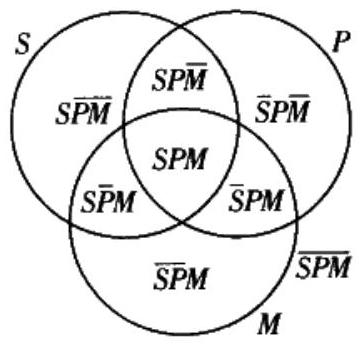
\includegraphics[max width=\textwidth, center]{2025_05_15_6a28331d5e7c993ad07ag-274}

图6-1\\
以瑞典人的类( $S$ )、农民的类( $P$ )和音乐家的类 $(M)$ 为例,可以作如下解释。SPM 是这三个类的积,由所有瑞典农民音乐家组成。SPM是前两个类与第三个类之补的积,由不是音乐家的瑞典农民组成。S $\bar{P} M$是第一、第三个类与第二个类之补的积:所有不是农民的瑞典音乐家组成的类。 $S \overline{P M}$ 是第一个类与其他两个类之补的积:所有不是农民也不是音乐家的瑞典人组成的类。接下来, $\bar{S} P M$ 是第二、第三个类与第一个类之

补的积:所有不是瑞典人的农民音乐家组成的类。 $\bar{S} P \bar{M}$ 是第二个类与其他两个类之补的积:所有不是瑞典人也不是音乐家的农民组成的类。 $\overline{S P M}$ 是第三个类与前两个类之补的积:所有不是瑞典人也不是农民的音乐家组成的类。最后,$\overline{S P M}$ 是三个类的补的积:所有不是瑞典人、不是农民,也不是音乐家的事物组成的类。

我们把注意力集中到标有 $P$ 和 $M$ 的两个圆上,显然,加上阴影或写人 $x$ 就能表示出 $P 、 M$ 构成的任何标准式直言命题,无论哪个是主项哪个是谓项。例如,要用图表示命题"所有 $M$ 是 $P$"$(M \bar{P}=0)$ ,我们就把所有不包含在 $P$ 中的 $M$ 的部分加上阴影。这个区域,包括了标有 $S \bar{P} M$ 和 $\overline{S P M}$ 的部分,这样就形成了图6-2。

我们再把注意力集中到 $S$ 和 $M$ ,加上阴影或写人 $x$ 就能表示由 $S$ 、 $M$ 构成的任何标准式直言命题,无论它们出现的顺序。要用图表示命题 "所有 $S$ 是 $M$"$(S \bar{M}=0)$ ,我们就把所有不包含在 $M$ 中的 $S$ 的部分加上阴影。这个区域,包括了标有 $S \overline{P M}$ 和 $S P \bar{M}$ 的部分。这样就形成了图 6-3。

现在,利用三个交叉的圆,就可以在一个图中同时表示两个命题——当然,条件是其中只出现三个不同的项。这样,"所有 $M$ 是 $P$"和"所有 $S$ 是 $M$"可以同时表示在图6-4中。\\
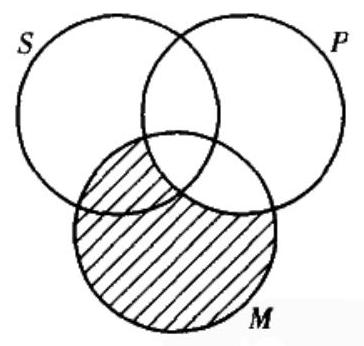
\includegraphics[max width=\textwidth, center]{2025_05_15_6a28331d5e7c993ad07ag-275(2)}

图6-2\\
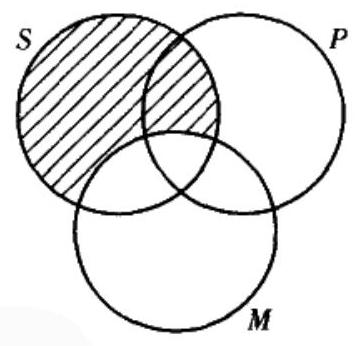
\includegraphics[max width=\textwidth, center]{2025_05_15_6a28331d5e7c993ad07ag-275(1)}

图6-3\\
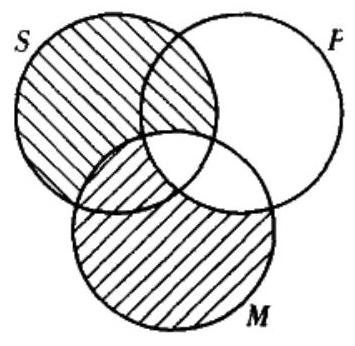
\includegraphics[max width=\textwidth, center]{2025_05_15_6a28331d5e7c993ad07ag-275}

图6—4

这正是三段论 AAA-1 的两个前提:

此三段论是有效的,当且仅当两个前提蕴涵或曰能推出结论,即两个前提已断言了结论所断言的东西。因此,在文恩图中画出有效论证的前提,也就已经把结论画出来了,而不需要画更多的圆。结论"所有 $S$ 是 $P$"的文恩图,应为在标有 $S \overline{P \bar{M}}$ 和 $S \bar{P} M$ 的部分加上阴影。我们看到表示两个前提的文恩图,也确实已经把结论表示了出来。这种情况说明 AAA- 1 一定是有效式。 ${ }^{[3]}$

我们再用文恩图检验一个明显无效的三段论:

所有狗是动物,\\
所有猫是动物,\\
所以,所有猫是狗。

用文恩图表示两个前提就是图6-5。\\
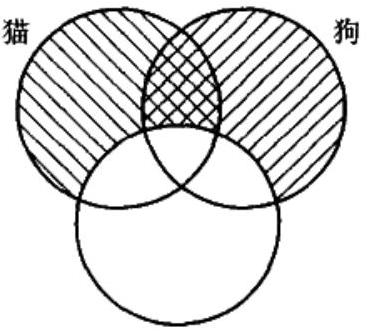
\includegraphics[max width=\textwidth, center]{2025_05_15_6a28331d5e7c993ad07ag-276}

动物

图6-5\\
在这个图中,$S$ 指称所有猫组成的类,$P$ 指称所有狗组成的类,而 $M$指称所有动物组成的类,$S \overline{P M} 、 S P \bar{M}$ 和 $\bar{S} P \bar{M}$ 部分已经加上了阴影,但结论却没有被表示出来,因为 $S \bar{P} M$ 部分没有阴影,要图示结论就必须把 $S \overline{P M}$ 和 $S \bar{P} M$ 两部分都加上阴影。这样,就能看出 AAA-2 的两个前提的图示并没能表示结论,这证明结论的断定超出了前提,前提并不蕴涵结论。而一个前提不蕴涵结论的论证是无效的,所以,我们所画出的图示证明了这个三段论是无效的。(实际上,它证明任何形如 AAA-2 的三段论都是无效的。)

如果我们用文恩图检验由一个全称前提和一个特称前提构成的三段论,那么,很重要的一点是:要首先在图中表明全称前提。举例来说,要

所有艺术家都是自我主义者,\\
有艺术家是乞亞,\\
所以,有乞丐是自我主义者。

我们应当先画出全称前提"所有艺术家都是自我主义者",再写人 $x$ 表示特称前提"有艺术家是乞丐"。正确的图示见图 6-6。\\
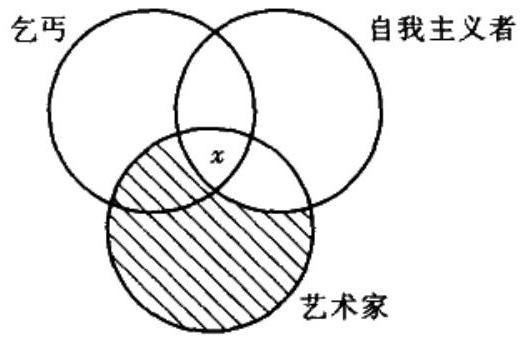
\includegraphics[max width=\textwidth, center]{2025_05_15_6a28331d5e7c993ad07ag-277}

图6-6\\
$S \bar{P} M$ 连同 $\overline{S P} M$ 两个部分表明的是全称前提,如果在给这两个部分加上阴影之前,试图先表明特称前提,我们就不能确定到底该把 $x$ 加在 $S P M$ 部分还是 $S \bar{P} M$ 部分,或者两个部分都加上。如果加在 $S \bar{P} M$ 当中,或者加在这部分与 $S P M$ 的交界处,那么加在 $S \bar{P} M$ 中的阴影就让图的原意变得含混不清。既然前提中包含的信息已经表示在图中了,检验时就看它是否也表明了结论。如果结论"有乞丐是自我主义者"能被表示出来,就应该把 $x$ 放在"乞甹"和"自我主义者"两个类的交叉部分。这个部分既包含了 SPM 也包含 SPM 部分,它们共同表明 SP。此三段论的结论所断定的东西,已经在表示前提的图示中表明了,因此,这个三段论是有效的。

再来看另一个例子,对这个例子的讨论将说明文恩图一个更重要的作用。考虑论证:

\begin{displayquote}
所有大科学家都是大学毕业生,有职业运动员是大学毕业生,
\end{displayquote}

首先在 $S P \bar{M}$ 和 $\bar{S} P \bar{M}$ 部分加上阴影,这样就表明了全称前提(见图6— 7),但我们仍然不明白应该把 $x$ 加到哪一部分才能表明特称前提。特称前提是"有职业运动员是大学毕业生",所以 $x$ 必须加在标有"职业运动员"和"大学毕业生"的两个圆交叉的部分。但是,交叉的区域又包括两个部分:$S P M$ 和 $S \bar{P} M$ 。 $x$ 应该放到其中哪个部分呢?前提并没有告诉我们答案,如果任意选一部分把 $x$ 加上去,就可能在图中加上了一些前提中本来没有的信息——也就破坏了文恩图检验的有效性。如果在两个部分都加一个 $x$ ,也会超出前提的断言。但是,把 $x$ 放在两部分的交界线上,我们就正好表明了第二个前提,而没有提供任何更多的东西。 $x$ 放在交界线上,指的是有东西属于它们两个类中的一个,但确实没有说明到底属于哪一类。两个前提的完整图示见图 6--8。\\
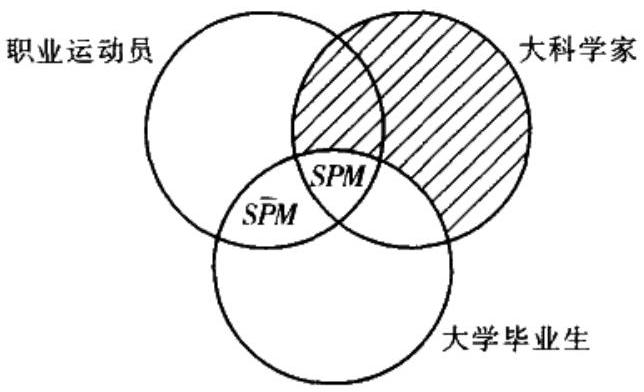
\includegraphics[max width=\textwidth, center]{2025_05_15_6a28331d5e7c993ad07ag-278}

图 6-7\\
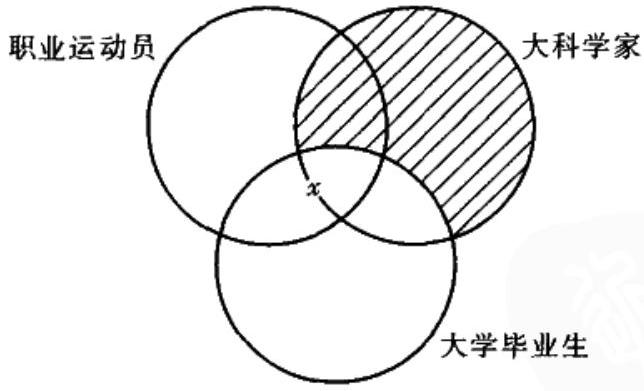
\includegraphics[max width=\textwidth, center]{2025_05_15_6a28331d5e7c993ad07ag-278(1)}

图6-8\\
通过考察,我们会发现前提的图示中并没有把结论表达出来。要表明结论"有职业运动员是大科学家",就必须要加一个 $x$ 在上面两个圆的交叉部分,或者加在 $S P \bar{M}$ 中,或者加在 $S P M$ 中。前面一个部分已经被加上阴影排除出去了,当然就不会包含 $x$ 。但图示也并没有显示 $S P M$ 中有 $x$ 。确实,\\
$S P M$ 或者 $S \bar{P} M$ 之中必有一个元素,但这个图示并没有说明究竟是在前者当中,还是在后者当中,因为前提就没有说明这一点。所以,结论就可能为假。当然,我们由此并不能确定结论就是假的,而只能知道结论没有被前提断定或蕴涵。但这已足以告诉我们论证是无效的。这个图也充分说明并非只有给定的这个三段论是无效的,而是所有形如 AII-2 的三段论都是无效的。

使用文恩图检验标准式三段论的一般做法可以总结如下:首先,在三圆的文恩图上标记三段论的三个项。接下来,把两个前提在图中都表示出来,如果一个前提是全称、另一个是特称的话,要首先标明全称前提。特别注意,如果特称前提并没有明确表明应该把 $x$ 加在哪一部分时,就把 $x$放在两个部分的交叉线上。最后,检查图示中是否已经包含了结论:如果包含了,那么三段论就是有效的,否则就是无效的。

使用文恩图区分三段论有效性与无效性的理论依据是什么?这个问题的答案可分为两个部分。首先,必须结合 6.2 节讲到的三段论论证的形式性质来讨论。那一节讲过,对给定三段论有效还是无效的一种合理检验是去判定另外一个三段论的有效性如何,而这个三段论与要考察的三段论恰有相同的形式。这种方法正是文恩图解法的基本依据。而说明文恩图解法如何达到这种检验目标,就构成问题解答的第二部分。

三段论一般都是就对象类而言的,其中的对象并不都呈现在我们面前,比如音乐家的类、大科学家的类、钠盐的类等等。这些类之间的包含或排斥关系可能是由论证得出的,也可能是在科学研究过程中经验地发现的。但它们绝不会自己呈现出来,因为涉及的类的元素不可能全部展现出来接受观察。但我们可创设一种情形,在这种经特殊界定的情形中,所涉及各个类的元素都可以呈现在人们面前以供直接观察,从而可以构造关于这种自设情形的三段论论证。文恩图本来是为表示标准直言命题而发明的,但其亦属于一种创设情形,一种可以使用各种工具在纸上、在黑板上绘制出来的情形。其所表示的命题亦可以解释为指涉图形本身。兹举一例即可说明。假如我们有这样一个关于分布在世界各地的各色人等的特殊三段论,其词项分别指称成功人士、热爱工作者和心猿意马者(工作中注意力分散者):

所有成功人士都是热爱工作者,没有热爱工作者是心猿意马者,

所以,没有心猿意马者是成功人士。

它的形式是 AEE-4,即:

所有 $P$ 是 $M$ ,\\
没有 $M$ 是 $S$ ,\\
$\therefore$ 没有 $S$ 是 $P$ 。

我们可以通过构造图6-9这样的文恩图来检验它,其中,$S P \bar{M}$ 和 $\bar{S} P \bar{M}$两部分加上了阴影表示第一个前提,$S \bar{P} M$ 和 $S P M$ 也加上了阴影表示第二个前提。\\
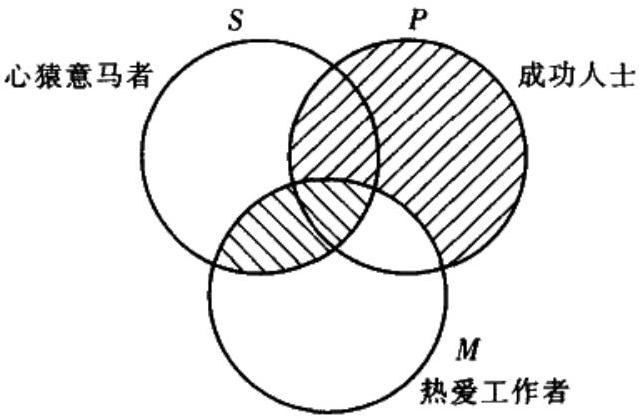
\includegraphics[max width=\textwidth, center]{2025_05_15_6a28331d5e7c993ad07ag-280}

图6-9\\
仔细观察这个图,可发现 $S P$(由 $S P M$ 和 $S P \bar{M}$ 组成)已经被阴影标明,因此,这个三段论的结论已经在图中表达出来了。那么,它是怎样表明这个三段论有效的呢?三段论论及的是几个相去甚远的对象的大类:很多人在工作中心猿意马,并且他们分布在世界各地,相互之间空间距离遥远。但是,我们却能构造出相同形式的三段论,其中所涉及的对象都是呈现在我们面前可供直接观察的。在上列文恩图中,这些对象就是标有 $S 、 M 、 P$ 的圆中没有加阴影的部分,这里有一个新的三段论:

所有 $P$ 圆中未加阴影的部分都是 $M$ 圆中未加阴影的部分,没有 $M$ 圆中未加阴影的部分是 $S$ 圆中未加阴影的部分,

所以,没有 $S$ 圆中未加阴影的部分是 $P$ 圆中未加阴影的部分。

这个新的三段论并没有涉及任何遥远的东西,而只涉及我们所创设的情形-一已经画好的文恩图的各个部分。这些类间相互包含与排斥的所有关系都呈现出来接受直接观察,因而可以逐一察看所有的可能。我们看到,所有是 $P$ 的部分都是 $M$ 的部分,而 $M$ 和 $S$ 没有共同的部分,所以 $S$和 $P$ 也就不可能有任何相同的部分。这里涉及的仅仅是图中的情形,因此可以说我们通过观察直接看出了这个三段论的有效性。由于上面关于各色人等的那个三段论,恰恰与这个三段论形式相同,根据三段论论证的形式性质,我们即可确认原来那个三段论也是有效的。这种说明也可解释文恩图解法为何可以证明一个无效三段论的无效性,同样也可通过直接检验一个具有相同形式但可在文恩图中直接显示的三段论,间接地检验待判定三段论。

\section*{练习题}
I.写出下列三段论的形式,分别用 $S$ 和 $P$ 代表结论的主、谓项,$M$代表中项,然后用文恩图解法加以检验。

\section*{例题}
1.AEE-1

\section*{解答}
题目已经告诉我们这是第一格的三段论,因此,中项 $M$ 在大前提中做主项、在小前提中做谓项,结论是 E 命题,记为:没有 $S$ 是 $P$ 。第一个前提(即大前提,其中含有结论的谓项)是 A 命题,记为:所有 $M$ 是 $P$ 。第二个前提(即小前提,其中含有结论的主项)是 E 命题,记为:没有 $S$是 $M$ 。因此,整个三段论的形式如下:

$$
\begin{aligned}
& \text { 所有 } M \text { 是 } P, \\
& \text { 没有 } S \text { 是 } M, \\
& \text { 所以, 没有 } S \text { 是 } P \text { 。 }
\end{aligned}
$$

其文恩图解检验见图 6-10,可表明此三段论无效。\\
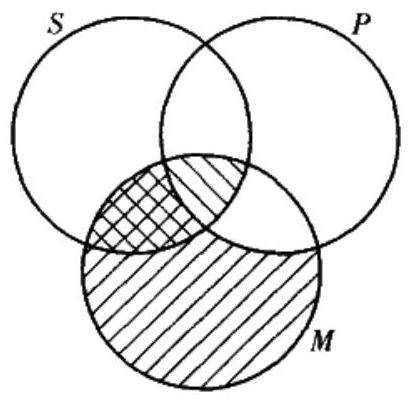
\includegraphics[max width=\textwidth, center]{2025_05_15_6a28331d5e7c993ad07ag-282}

图6-10\\
2. $\mathrm{EIO}-2$\\
3.OAO-3\\
4. $\mathrm{AOO}-4$\\
5. $\mathrm{EIO}-4$\\
6.OAO-2\\
7. $\mathrm{AOO}-1$\\
8.EAE-3\\
9.EIO-3\\
10.IAI-4\\
11. $\mathrm{AOO}-3$\\
12.EAE-1\\
13.IAI-1\\
14.OAO-4\\
15.EIO-1

II.把下列各三段论转化为标准形式,给出它们的格与式,并用文恩图加以检验。\\
*1.有改革者是狂徒,所以有理想主义者是狂徒,因为所有改革者是理想主义者。

2.有哲学家是数学家,因为有科学家是哲学家,而所有科学家是数学家。

3.有哺乳动物不是马,因为没有马是人头马,所有人头马是哺乳动物。\\
4.有神经病人不是被监护人,但所有罪犯是被监护人,所以可知有神经病人不是罪犯。\\
*5.所有水下船只是潜水艇,因此,没有潜水艇是游艇。因为没有游艇是水下船只。

6.从来没有罪犯是拓荒者,因为所有罪犯是恶人(unsavory),而从来没有拓荒者是恶人。

7.没有音乐家是宇航员,所有音乐家是篮球迷,因此,没有宇航员是篮球迷。

8.有基督徒(Christians)不是卫理公会派教徒(Methodists),因为有基督徒不是新教徒(Protestants),而有新教徒不是卫理公会派教徒。

9.没有想赢得大选的人是真正的自由党人,所有活跃的政客是想赢得大选的人,从这两个前提可以推出,没有真正的自由党人是活跃的政客。\\
*10.没有怯懦者是工人领导,因为没有怯懦者是真正的自由党人,并且所有工人领导是真正的自由党人。

\section*{6.4 三段论规则和三段论谬误}
在许多情况下,一个三段论并不能真正推得其结论。为帮助人们避免常见的错误,人们制定了一系列规则(本书列出六条)用来范导论证:对于任何给定的标准式三段论,通过考察其中是否有违反规则的情况,就能对它进行评判。

违反任何一条规则都会导致错误。这是一种特殊种类的论证错误,所以我们称之为三段论谬误;又因为这种错误是论证形式方面的,所以称之为形式谬误(与第4章所讲非形式谬误相对照)。在三段论论证中,必须谨防违反规则,避免产生谬误。每一种形式谬误都有一个传统名称,以下详加介绍。

\section*{规则1 避免四项}
一个有效的标准式直言三段论必须仅仅包含三个项,在整个论证中,每一个项都须在相同的意义上使用。

在直言三段论中,结论断定了两个项即主项(小项)与谓项(大项)之间的关系。因此,只有前提断定的是这两个项分别与同一个第三项(中项)的联系时,结论才能是合理的。如果前提不能做到这一点,就不能在结论的两个项之间建立联系,论证就不能进行。所以,每个有效的直言三段论必须只有三个项——不能多也不能少。如果包含了多于三个的项,三段论就是无效的。这种谬误叫做四项谬误。

这种谬误通常源于语词歧义,即用同一个词或短语表达两种不同的含义。最常见的是中项的含义发生转换,同一个词以某种用法与小项发生联系,而以另一种用法与大项发生联系。这样一来,与结论中的两个项发生联系的是两个不同的项(而不是同一个中项),所以结论断定的关系也就不能成立。 ${ }^{[4]}$

本章开始定义"直言三段论"时,就指出每一个三段论一定有且只有三个项。 ${ }^{[5]}$ 所以,可以把这个规则("避免四项")看做是一个论证成为一个真正的三段论的保证。

\section*{规则2 中项至少在一个前提中周延}
如果(如 5.3 节所说明)命题述及一个项所指称的全部对象,该项在命题中就是"周延"的。如果中项在两个前提中都不周延,推出结论所需要的词项关联就不能建立。

历史学家芭芭拉•塔克曼(Barbara Tuchman)认为,许多无政府主义的早期批判家是以下面这样一个"无意识的三段论"为依据进行论证的。

\begin{displayquote}
所有俄国人是革命者,所有无政府主义者是革命者,
\end{displayquote}

\begin{displayquote}
所以,所有无政府主义者是俄国人。 ${ }^{[6]}$
\end{displayquote}

这个三段论显然是无效的。错误在于它根据无政府主义者、俄国人两个类分别与革命者的类之间的联系,断定了前两个类的关系——但革命者这个项在两个前提中都是不周延的。第一个前提没有述及全部革命者,第二个前提同样没有。"革命者"在论证中做中项,如果它在三段论两个前提中都不周延,那么三段论就不可能是有效的。这样的谬误叫做中项不周延谬误。

这个规则的依据是小项和大项之间的联系需要中项做中介。而要建立这种联系,结论的主项或者谓项就必须与中项所指称类的全部对象相关联。否则,结论中的两个项就有可能分别与中项的不同部分发生联系,因而不必然与另一个项相关联。

这恰好是上面给出的三段论所存在的问题。俄国人只包含在革命者类的一部分当中(据第一个前提),无政府主义者也只是包含在革命者类的一部分之中(据第二个前提)——这两部分却是与另一个类(三段论的中项)的不同部分发生联系的,所以,中项就不能成功地联结小项和大项。一个有效的三段论,其中项必定至少在一个前提中周延。

规则 3 在结论中周延的项在前提中也必须周延\\
述及一个类的全部对象,比述及其中某些对象要断定更多。所以,如果三段论前提中不周延的项在结论中周延,也就是结论断定了比前提更多

的东西。但是,有效的论证要求其前提必须能逻辑地推出结论,结论绝不能比前提断定得更多。可以说,在结论中周延而在前提中不周延的项确实是个信号,说明结论超出了前提,跑得太远了。这种谬误叫做不当周延。

结论可能是小项(主项)超出了前提,或者大项(谓项)超出了前提。所以,不当周延有两种不同形式,我们分别给它们一个名字:

大项不当周延("非法大项"),\\
小项不当周延("非法小项")。\\
举个例子来说明第一种,看下面这个三段论:

\begin{displayquote}
所有的狗是动物,没有猫是狗,
\end{displayquote}

\begin{displayquote}
所以,没有猫是动物。
\end{displayquote}

很明显,这个论证是不对的,但错在哪里呢?就错在结论是对所有动物的断言,即结论断定的是所有动物都在猫的类之外,而前提并没有对所有动物做出断言——故结论不当地超出了前提的断定。由于"动物"在三段论中做大项,所以此处的谬误就是非法大项。

再举个例子来说明第二种,看下面这个三段论:

所有传统教徒都是原教旨主义者(fundamentalist),所有传统教徒都是宽容筀胎行为的,

所以,所有宽容塈胎行为的都是原教旨主义者。

我们立刻会感觉到这个论证也有问题,其错误就在于:结论断定了所有堕胎行为的宽容者,而在前提中并没有这样的断言,没有述及所有宽容堕胎行为者的情况。这样,结论就不能为前提所担保。这个例子中"宽容堕胎行为的"是小项,所以此处的谬误就是非法小项。

\section*{规则4 避免出现两个否定前提}
任何否定命题( $\mathbf{E}$ 或 $\mathbf{O}$ )都否认类的包含关系,断定一个类的部分或者全部被排除在另一类的全体之外。但是,由两个断定这种排斥性的前提不能得出结论中的联系,因此,不可能是有效的论证。这种错误叫做排斥

前提谬误。\\
理解这个谬误需要进一步思考。考虑三段论的小项 $S$ 、大项 $P$ 和中项 $M$ ,对于这三个项之间的联系,两个否定前提能告诉我们什么呢?它们说明 $S$(结论的主项)完全或部分地排斥 $M$(中项)的一部分或者全部,并且 $P$(结论的谓项)完全或部分地排斥 $M$ 的一部分或者全部。但是,不管 $\boldsymbol{S}$ 和 $\boldsymbol{P}$ 的关系如何,这些关系中的任何一个都可能成立。这样的否定前提不能告诉我们 $S$ 和 $P$ 之间究竟是包含还是排斥,究竟是全部地包含或排斥,还是部分地包含或排斥。因此,如果三段论的两个前提都是否定的,论证肯定是无效的。

规则5 如果有一个前提是否定的,那么结论必须是否定的\\
如果结论是肯定的,也就是说,如果它断言两个类中的一个( $S$ 或 $P$ )完全或部分地包含在另一个之中,那么,前提必须断定这样的第三个类存在才能推出结论,即第三个类必须包含第一个并且被第二个包含,而类之间的这种包含关系只能由肯定命题表示。所以,肯定的结论只能由两个肯定的前提得到。违反这条规则的错误叫做从否定推肯定谬误。

要想得出肯定结论必须要有两个肯定前提,如上所述,我们可以确定地说,只要两个前提中有一个是否定的,结论就必须也是否定的,否则论证无效。

与其他谬误不同,这个谬误并不常见,因为对于任何从否定前提得肯定结论的论证,很容易就可以看出是极不合理的。举一个例子就能说明:

\begin{displayquote}
没有诗人是会计,有艺术家是诗人,
\end{displayquote}

所以,有艺术家是会计。

立即可以看到,由第一个前提对诗人和会计的排斥关系的断言,已使得该论证不可能为艺术家和会计之间的包含关系提供任何有效辩护。

规则 6 两个全称前提得不出特称结论\\
在直言三段论的布尔解释中(见5.6节),全称命题(A和E)没有存在含义,但特称命题( $\mathbf{I}$ 和 $\mathbf{O}$ )却有存在含义。只要像本书这样设定了布尔解释,就要避免从没有存在含义的前提得出有存在含义的结论。

最后这个规则在传统逻辑或者亚里士多德逻辑对直言三段论的解释中

并不需要,因为它们并不关心存在含义问题。但是,仔细考虑一下预设问题就会很清楚,如果一个论证的前提根本没有断定什么东西存在,但是从这些前提却推出了有些东西的存在,那么结论就是不合理的。这种错误叫做存在谬误。

下面这个例子就犯有这种谬误:

所有宠物都是家养动物,没有独角兽是家养动物,

所以,有独角兽不是宠物。

假如这个论证的结论是全称的"没有独角兽是宠物",它是完全有效的。在传统解释下,由于全称命题与特称命题一样都有存在含义,例子中的结论只是上述有效论证结论的"下位"。

但从布尔解释的角度说,上例的结论("有独角兽不是宠物")不仅仅是个"下位",因为特称命题与全称命题有很大不同。结论是特称的 $\mathbf{O}$ 命题,有存在含义,而 $\mathbf{E}$ 命题("所有独角兽不是宠物")是没有存在含义的。传统观点下接受的推论在布尔解释下不再被接受,因为在后者看来这样的论证犯了存在谬误一一种在传统解释下不会出现的错误。 ${ }^{[7]}$

以上给出的六条规则只适用于标准式直言三段论。它们提供了足够的工具,用以检验这一领域内任何论证的有效性。对于任一标准式直言三段论,如果违反了任一规则就是无效的,如果遵循了所有的规则就一定是有效的。

\section*{6. 5 直言三段论的 15 个有效形式}
三段论的式取决于其中所含三个命题的类型(A、E、I、O)。直言三段论有 64 个不同的式,即这三个命题的 64 种可能组合:AAA、AAI、 AAE 等等,一直到 $\cdots \cdots$ EOO $、 \mathrm{OOO}$ 。

三段论的格是其逻辑形状,由中项在前提中的不同位置决定。所以一共有四种不同的格,如果头脑中有一个图表或者用图标说明,就可以很清晰地记住这几个格,见图6—11:\\
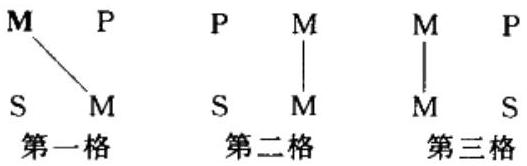
\includegraphics[max width=\textwidth, center]{2025_05_15_6a28331d5e7c993ad07ag-288}

图6-11\\
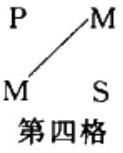
\includegraphics[max width=\textwidth, center]{2025_05_15_6a28331d5e7c993ad07ag-288(1)}

从图中可见:

\begin{itemize}
  \item 第一格的中项是大前提的主项、小前提的谓项;
  \item 第二格的中项在两个前提中都做谓项;
  \item 第三格的中项在两个前提中都做主项;
  \item 第四格的中项是大前提的谓项、小前提的主项。
\end{itemize}

64 个式都可以有四个格。把两者结合起来,给定了三段论的式与格,也就唯一地确定了三段论的形式。因此,标准式直言三段论恰有 $256(64 \times 4)$个可能的形式。

这些形式中绝大部分是无效的。根据前一节阐明的三段论规则,我们可以排除那些违反了一条或几条规则的形式,剩下的就是直言三段论的有效式。 256 个形式中,只有 15 个形式不能被排除,因而它们是有效的。 ${ }^{[8]}$

为更好地掌握三段论,古典逻辑学家给每一个有效式都起了独特的名称,每一个都完全刻画了其格与式。了解有效式的这个小集合,记住每一个有效形式的名称,对于我们实际运用三段论论证是很有帮助的。这些名称都是精心设计的,每个名称都包含了三个元音,代表着被命名三段论的式(依据标准的顺序:大前提、小前提、结论)。对于同式不同格的有效三段论形式,都分别给它们指派唯一的名称。例如,对于式为 EAE 的三段论,如果是第一格的就叫做 Celarent,而如果是第二格的就叫做 Cesare。 ${ }^{[9]}$

这些名称曾经有(现在仍然有)很实用的功能:如果懂得只有式与格的某些特定组合是有效的,并且通过名字就能识别那些有效论证,那么,无论给出任何式或格的三段论,就都能立即判定其正误。例如,AOO 式只在第二格才是有效的。这个唯一的形式(AOO-2)就叫做 Baroko。 ${ }^{[10]}$熟悉 Baroko 并能很容易指认它的人就会确信这个式的其他格都是无效的,是必须拒斥的。

古典逻辑学家很细致地研究了这些形式,谙熟它们的结构和逻辑"感

应"。这种精心设计好的逻辑系统,会使得一个人在言语或文本中碰到三段论论证时,能立即确切指认哪些是有效的,哪些是无效的。许多世纪以来,逻辑训练的一种常用方式,就是通过给出三段论有效形式的名称,来为三段论论证的可靠性进行辩护。而在激烈的日常论辩中具备这种迅速识别有效论证与无效论证的能力,一直被视为富有学养、思维敏锐的标志。而依赖演绎论证所建立起来的论证链条之坚固也得到了充分显示。一旦完全掌握三段论理论,这种实际论辩能力就会得到富有成效的令人愉悦的提升。

三段论论证曾经有如此广泛的应用,并被普遍视为学术论证最不可缺少的工具,因此,最先系统论述三段论理论的学术大师亚里士多德,得到了人们上千年的尊崇。他关于三段论的分析的论集迄今仍沿用着一个简单但令人肃然起敬的名字:Organon,即《工具论》。

作为这个著名逻辑体系的初学者,我们对三段论的掌握可能难以非常精通。但列出所有有效三段论形式并加以熟练掌握,无疑是最为有用的。 15 个有效三段论形式(布尔解释下的)可以根据格的不同分为四组:在前三个格中都有四个有效形式,第四格有三个有效形式。 ${ }^{[11]}$

下图即列出了 15 个有效形式,以及它们相应的传统名称:

\section*{标准式直言三段论的 15 个有效形式}
第一格(中项在大前提中做主项、在小前提中做谓项):\\
1.AAA-1 Barbara\\
2.EAE-1 Celarent\\
3.AlI-1 Darii\\
4.EIO-1 Ferio\\
第二格(中项在两个前提中都做谓项):\\
5.AEE-2 Camestres\\
6.EAE-2 Cesare\\
7.AOO-2 Baroko\\
8.EIO-2 Festino\\
第三格(中项在两个前提中都做主项):\\
9.All-3 Datisi\\
10.IAI-3 Disamis\\
11.EIO-3 Ferison\\
12.OAO-3 Bokardo

第四格(中项在大前提中做谓项、在小前提中做主项):\\
13.AEE-4 Camenes\\
14.IAI-4 Dimaris\\
15.EIO-4 Fresison

\section*{练习题}
I.指出下列无效的三段论形式违反了哪条规则,犯了何种谬误。

\section*{例题}
1.AAA-2

\section*{解答}
第二格三段论的中项在大、小前提中都做谓项。如果一个第二格三段论由三个 A 命题组成,那么,它一定是:所有 $P$ 是 $M$ ,所有 $S$ 是 $M$ ,所以,所有 $S$ 是 $P$ 。其中,中项 $M$ 在两个前提中都不周延,因此,从这样的前提不能有效地推出所有 $S$ 是 $P$ 。形如 AAA-2 的三段论都违反了中项至少在一个前提中周延的规则,犯了中项不周延的谬误。\\
2.EAA-1\\
3. $\mathrm{IAO}-3$\\
4.OEO-4\\
*5.AAA-3\\
6.IAI-2\\
7.OAA-3\\
8.EAO-4\\
9.OAI-3\\
*10.IEO-1\\
11.EAO-3\\
12.AII-2\\
13.EEE-1\\
14.OAO-2\\
*15.IAA-3

II.指出下列无效的三段论违反了什么规则,犯了何种谬误。

\section*{例题}
1.所有课本是需要认真研读的书,有参考书是需要认真研读的书,所以,有参考书是课本。

\section*{解答}
在此三段论中,"课本"是大项(结论的谓项),"参考书"是小项 (结论的主项),而"需要认真研读的书"在两个前提里都出现了,因而它

是中项。但是,中项在两个前提中都不周延,所以这个三段论违反了中项至少在一个前提中周延的规则,犯了中项不周延的谬误。

2.所有 criminal action(犯罪行为)是恶行,所有谋杀指控是 criminal action(刑事诉讼),

所以,所有谋杀指控是恶行。\\
3.没有悲剧演员是白痴,有喜剧演员不是白痴,

所以,有喜剧演员不是悲剧演员。\\
4.有鹦鸦不是害鸟,所有鹦鹉是宠物,

所以,没有宠物是害鸟。\\
*5.所有永动机是全效的机器,所有全效的机器是无摩擦的机器,

所以,有无摩擦的机器是永动机。\\
6.有优秀演员不是大力士,所有职业摔跤运动员是大力士,

所以,所有职业摔跤运动员是优秀演员。\\
7.有的钻石是珍贵的石头,有的碳化合物不是钻石,

所以,有的碳化合物不是珍贵的石头。\\
8.有的钻石是珍贵的石头,有的碳化合物是钻石,

所以,有的碳化合物不是珍贵的石头。\\
9.所有钱极的人是吃得最多的人,所有吃得最少的人是饿极的人,所以,所有吃得最少的人是吃得最多的人。\\
*10.有哈巴狗不是好猎犬,所有哈巴狗是脾气温和的狗,

III.指出下列三段论中哪些是无效式,它们违反了什么规则,犯了何种谬误。

\section*{例题}
1.所有巧克力棒是高脂肪食品,因为所有巧克力棒是甜腻食物,而有高脂肪食品不是甜腻食物。

\section*{解答}
此三段论的结论是肯定的(所有巧克力棒是高脂肪食品),但有一个前提是否定的(有高脂肪食品不是甜腻食物),因而是无效的。违反了 "如果有一个前提是否定命题,那么结论必须是否定命题"的规则,犯了从否定推肯定谬误。

2.所有发明家是能找到常见物之新模型的人,所以所有发明家是行为古怪的人,因为所有行为古怪的人是能找到常见物之新模型的人。

3.有蛇不是危险动物,但所有蛇是爬行动物,因此,有危险动物不是爬行动物。

4.有含铁食物是有毒物质,因为所有含汞的鱼是含铁食物,而含汞的鱼是有毒物质。\\
*5.所有愤然批判国会自由主义头目的人是反对变革政治经济基本制度的人。所有右翼极端分子是反对变革政治经济基本制度的人,由此可知,所有愤然批判国会自由主义头目的人是右翼极端分子。

6.没有写狠琐的刺激性文章的人是诚实高尚的,有记者不是写猥琐的刺激性文章的人,因此,有记者是诚实高尚的。

7.所有拥护人民政府的人是民主主义者,所以,所有拥护人民政府的人是共产党的拥护者,因为所有民主主义者是共产党的拥护者。

8.没有煤焦油提取物是有营养的食物,因为所有人工色素是煤焦油提取物,没有人工色素是有营养的食物。

9.没有煤焦油提取物是有营养的食物,因为没有煤焦油提取物是天然作物,所有天然作物是有营养的食物。\\
*10.所有住在伦敦的人是饮茶的人,所有饮茶的人是喜欢它的人,由此可知所有住在伦敦的人是喜欢它的人。

N. 6.3 节末尾的第II题中有 10 个三段论,我们已经用文恩图进行了检验,发现其中 $1 、 4 、 6 、 7$ 和 10 是有效式,它们的名称各是什么?

例解\\
第1个是(IAI-3),即 Disamis。

\section*{6.6 直言三段论 15 个有效形式的演绎推导}
直言三段论的 15 个有效形式是从 256 个可能形式中排除无效式以后得以确立的。我们可以通过确定哪些形式违反了三段论的基本规则来实行这种排除——演绎推导出三段论的 15 个有效形式。

对逻辑初学者来说,不必一定弄清如何排除无效式的细节。但对于那些从三段论分析的复杂性中获取乐趣的人而言,这应是一种虽有难度但令人愉悦的挑战。如果只想认识和把握三段论的有效式,即 6.5 节讲到的那些内容,就可以绕过本节不看。

这种演绎推导并不那么容易理解。从事这项工作必须清晰地记住以下两点:(1)6.4 节设定的六条三段论基本规则;(2)三段论四个格的模式,即图6-11。

根据结论的不同形式,我们首先把三段论的所有可能形式分为四组。每个结论都是 A、E、I、O 四种直言命题之一,没有其他可能,据此可以分四种情形考察一个有效的三段论需要具备什么特性,即可以这样提问:如果结论是 A 命题,通过某一条或几条规则能够排除什么形式;如果结论是 E 命题可以排除什么形式,以此类推。下面我们就逐个进行考察。

\section*{情形1:如果三段论的结论是 $\mathbf{A}$ 命题}
在这种情形下,前提不可能是 E 命题,也不可能是 O 命题,因为如果前提为否定命题的话,结论就应该是否定的(规则5)。所以,两个前提必定是 A 命题或 I 命题。小前提不能是 I 命题,因为小项(结论的主项,也就是一个 A 命题的主项)在结论中是周延的,如果小前提是 I 命题,那么在前提中不周延的项在结论中周延,违反了规则 3 。两个前提,即大前提和小前提,不能是 I 和 A,因为如果是的话,有两种可能,或者是在结论中周延的项在前提中不周延,违反规则 3 ,或者是中项两次不周延,违反规则2。所以两个前提(结论是 A 命题时)必须都是 A 命题,这意味着唯一有效的形式是 AAA 式。而第二格的 AAA 式会使中项两次不周延,第三格和第四格的 AAA 式都会造成前提中不周延的项在结论中周

延的错误。所以,如果三段论的结论是 A 命题,唯一的有效形式就是第一格的 AAA 式,即 AAA-1,传统上称这个有效形式为 Barbara。

情形 1 的总结:如果三段论的结论是 $\mathbf{A}$ 命题,只能有一种有效形式:\\
AAA-1-Barbara。

\section*{情形2:如果三段论的结论是 $\mathbf{E}$ 命题}
E 命题的主项和谓项都是周延的,因此,如果结论为 E 命题,三段论前提中的三个项也都必须至少周延一次 ${ }^{(1)}$ ,这只有当前提之一也是 E 命题时才有可能。但不能两个前提都是 E 命题,因为不能允许两个否定前提 (规则 4),同理可知另一个前提也不能是 O 命题。另一个前提也不能是 I命题,否则在结论中周延的项在前提中不周延,违反规则 3 。这样,另一个前提必须是 A 命题,两个前提的组合可能是 AE 或 EA。因此,在结论是 E 命题的情况下,可能的正确形式为 AEE 和 EAE。

如果是 AEE 式,它不能是第一格,也不能是第三格。因为如果是这两个格的话,结论中周延的项在前提中不周延。所以,有效的AEE式只能是第二格的,即AEE-2(传统上称为 Camestres),或者是第四格的,即 AEE-4(传统上称为 Camenes)。如果是 EAE 式,它不能是第三格,也不能是第四格,因为那也都导致结论中周延的项在前提中不周延。所以,有效的 EAE 式只能或者是第一格的,即 EAE-1(传统上称为 Celarent),或者是第二格的,即 EAE-2(传统上称为 Cesare)。

情形 2 的总结:如果三段论的结论是 $\mathbf{E}$ 命题,只能有四种有效形式: AEE-2、AEE-4、EAE-1 和 EAE-2——分别是 Camestres、Camenes、Celar- ent 和 Cesare。

\section*{情形3:如果三段论的结论是 I命题}
在这种情形下,前提不能是 E 或 O 命题,因为如果有一个否定前提的话,结论也应该是否定的。两个前提也不能都是 A 命题,因为结论为特称的三段论其前提不能都是全称的(规则 6)。同样,两个前提也不能都是 I 命题,因为中项必须至少在一个前提中周延(规则 2 )。这样,前提的组合必须是 AI 或者 IA,因而结论为 I 命题的三段论可能的有效形式为 AII 和 IAI。

AII 在第二格和第四格中不可能有效,因为中项至少要周延一次。因

\footnotetext{(1)据规则 $2 、 3$ 。
}此保留下来的 AII 式就是 AII-1(传统上称为 Darii)和 AII-3(传统上称为 Datisi)。如果是 IAI 式,它不能是 IAI-1 和 IAI-2,因为这两个形式都违反中项至少在一个前提中周延的规则。剩下的有效形式就是 IAI-3(传统上称为 Disamis)和 IAI-4(传统上称为 Dimaris)。

情形 3 的总结:如果三段论的结论是 I 命题,只能有四种有效形式: AII-1、AII-3、IAI-3 和 IAI-4——分别是 Darii、Datisi、Disamis 和 Dima- ris。

\section*{情形4:如果结论是 $\mathbf{O}$ 命题}
在这种情形下,大前提不能是 I 命题,因为结论中周延的项在前提中也必须周延。所以大前提可能是 A 命题、 E 命题或者 O 命题。

假设大前提是 A 命题。这样,小前提就不能是 A 命题和 E 命题,因为结论为特称( O 命题)时,前提不能都是全称的。小前提也不能是 I 命题,否则,或者中项一次也不周延(违反规则 2 ),或者结论中周延的项在前提中不周延。因此,如果大前提是 A 命题,小前提必须是 O 命题,结果就是 AOO 式。但在第四格, AOO 式不可能有效,因为中项两次不周延。在第一格和第三格也不可能有效,因为结论中周延的项在前提中不周延。因此当大前提是 A 命题时, AOO 式保留下来的有效形式只有第二格 AOO-2(传统上称为 Baroko)。

再假设(如果结论是 O 命题)大前提是 E 命题。在这种情况下,小前提将不能是 E 命题或 O 命题,因为不允许两个否定前提。小前提也不能是 A 命题,因为结论如果为特称的,前提就不能是两个全称命题(规则6)。因而只剩下了 EIO 式——它在四种格中都是有效的,传统上分别叫做 Ferio(EIO-1)、Festino(EIO-2)、Ferison(EIO-3)和 Fresison ( $\mathrm{EIO}-4$ )。

最后,假设大前提是 O 命题。同样小前提也不能是 E 命题或 O 命题,因为不能允许两个否定前提。小前提也不能是 I 命题,因为那样的话,或者中项一次都不周延,或者结论中周延的项在前提中不周延。因此,如果大前提是 O 命题,小前提必须是 A 命题,即必为 OAO 式。但要排除 $\mathrm{OAO}-1$ ,因为中项两次都不周延。也要排除 OAO-2 和 OAO-4,因为这两种情况都会使结论中周延的项在前提中不周延。于是就只剩下一个有效形式 OAO-3(传统上称为 Bokardo)。

情形4的总结:如果结论是 O 命题,则有六个有效形式:AOO-2、

\section*{EIO-1、EIO-2、EIO-3、EIO-4 和 OAO-3,分别叫做 Baroko、Ferio、Festi- no、Ferison、Fresison 和 Bokardo。}
以上的分析通过排除法证明了直言三段论恰有 15 个有效形式:结论是 A 命题时有 1 个,结论是 E 命题时有 4 个,结论是 I 命题时有 4 个,而结论为 O 命题时有 6 个。这 15 个有效形式中,四个是第一格的,四个是第二格的,四个是第三格的,三个是第四格的。这样,就完成了标准式直言三段论的 15 个有效形式的演绎推导。

\section*{练习题}
对于乐于深人分析三段论的同学来说,结合 6.4 节给出的规则进行系统的分析,就可以找到下面几个理论问题的答案。而学过 6.6 节,掌握了有效三段论形式的演绎推导之后,就更容易了。注意要考虑到各种可能情况。

\section*{例题}
1.如果一个标准式直言三段论只有三个项,且这三个项在三段论中每次出现都周延,请问这样的三段论是否有效?

\section*{解答}
这样的三段论不可能是有效的。如果三个项在三段论中每次出现都周延,那么,组成三段论的三个命题必定都是 E 命题,其式必为 EEE ,违反了规则 4 ,即两个否定前提不能得结论。

2.结论为特称命题的第一格标准式直言三段论能否为有效式,如果有的话,可能是哪个或哪些式?

3.一个有效的标准式直言三段论的大项和小项能否都周延,如果能的话,可能是哪个或哪些格?

4.一个有效的标准式直言三段论的两个前提能否都是特称命题,如果能的话,可能是哪个或哪些格?\\
*5.一个有效的标准式直言三段论中能否只有一个项周延,并且只周延一次,如果能的话,可能是哪个或哪些格?

6.一个有效的标准式直言三段论能否只有两个项周延且每个周延一次,如果能的话,可能是哪个或哪些式?

7.一个有效的标准式直言三段论能否是两个前提为肯定命题,而结

论为否定命题,如果能的话,可能是哪个或哪些式?\\
8.一个有效的标准式直言三段论能否同时有一个特称前提和一个全称结论,如果能的话,可能是哪个或哪些格?

9.结论为全称的第二格标准式直言三段论能否为有效式,如果能的话,可能是哪个或哪些式?\\
-10.一个有效标准式直言三段论的中项能否在前提中都周延,如果能的话,可能是哪个或哪些格?

11.一个有效的标准式直言三段论能否有一个项在前提中周延,在结论中不周延?

\section*{第6章概要}
第6章考察标准式直言三段论:组成成分、形式、有效性和制约其正确使用的规则。

6. 1 节给出了三段论大项、小项和中项的定义:

\begin{itemize}
  \item 大项:结论的谓项
  \item 小项:结论的主项
  \item 中项:两个前提中都出现,但结论中不出现的第三个项
\end{itemize}

继而又分别定义了大前提和小前提,包含大项的前提叫做大前提,包含小项的前提叫做小前提。如果几个命题出现的次序正好是:大前提在第一位、小前提在第二位、结论在最后,我们就把这样的三段论指定为标准式的。\\
6.1 节也说明了三段论的式与格是如何确定的。

三段论的式由识别三个命题类型的字母来确定,即A、E、I、O中的三个。总共有 64 个不同式。

三段论的格由中项在前提中的不同位置来确定。对四个可能的格描述并定义如下:

第一格:中项在大前提中做主项、在小前提中做谓项。\\
模式为:$M-P, S-M$ ,所以 $S-P$ 。\\
第二格:中项在两个前提中都做谓项。\\
模式为:$P-M, S-M$ ,所以 $S-P$ 。\\
第三格:中项在两个前提中都做主项。

模式为:$M-P, M-S$ ,所以 $S-P$ 。\\
第四格:中项在大前提中做谓项、在小前提中做主项。\\
模式为:$P-M, M-S$ ,所以 $S-P$ 。\\
6.2 节说明了标准式三段论的式与格如何共同地确定其逻辑形式。由于 64 个式每一个都有四个格,所以共有 256 个标准式的直言三段论,但其中只有一小部分是有效式。

6. 3 节介绍检验三段论有效性的文恩图方法,即在几个交叉的圆中,作上恰当的标记或涂上阴影以表示前提的含义。\\
6.4 节阐明标准式三段论的六条基本规则,同时定义了违反各条规则所造成的谬误。\\
-规则 1 一个有效的标准式直言三段论必须仅仅包含三个项,在整个论证中,每一个项都须在相同的意义上使用。

违反本规则所犯的错误:四项谬误。\\
-规则 2 在一个有效的标准式直言三段论中,中项必须至少在一个前提中周延。

违反本规则所犯的错误:中项不周延谬误。\\
-规则 3 在一个有效的标准式直言三段论中,在结论中周延的项在前提中也必须周延。

违反本规则所犯的错误:大项不当周延谬误,或者小项不当周延谬误。\\
-规则 4 任何有两个否定前提的标准式三段论都不是有效的。\\
违反本规则所犯的错误:排斥前提谬误。\\
-规则 5 如果一个标准式三段论有一个前提是否定的,那么结论必须是否定的。

违反本规则所犯的错误:从否定推肯定谬误。\\
-规则 6 一个有效的标准式直言三段论,如果结论为特称命题,那么其前提不能都是全称的。

违反本规则所犯的错误:存在谬误。\\
6. 5 节给出了标准式直言三段论的 15 个有效形式的说明,识别它们的格与式,并说明了它们传统的拉丁名称:

AAA-1(Barbara)、EAE-1(Celarent)、AII-1(Darii)、EIO-1(Fe- rio)、AEE-2(Camestres)、EAE-2(Cesare)、AOO-2(Baroko)、EIO-2\\
(Festino)、AII-3(Datisi)、IAI-3(Disamis)、EIO-3(Ferison)、OAO-3 (Bokardo)、AEE-4(Camenes)、IAI-4(Dimaris)、EIO-4(Fresison)。

6. 6 节展示了 15 个有效形式的演绎推导,通过排除法程序,证明了只有 15 个形式是完全遵守三段论的六条基本规则的。

\section*{【注释】}
[1]这种区别是很大的。在上面的例子中,三段论(B)是有效推理,但三段论 (A)不是有效推理。\\
[2]此处我们假设构成命题本身都是偶真的,也就是说,既不是逻辑真的(例如 "所有软椅都是椅子"),也不是逻辑假的(例如"有软椅不是椅子")。因为如果它包含逻辑假的前提或逻辑真的结论,那么,不管三段论的形式如何,这个推理就可能是有效的——其有效性是说逻辑上不可能出现前提真而结论假的情况。我们也假设,三段论各项之间的逻辑联系仅仅是由其前提断定或推出的。作这些约束,目的是限定本章的考察范围,接下来讲的只是三段论论证,而不涉及其他类型的论证。把握其他论证的有效性或许依赖于更加复杂的逻辑研究。\\
[3]像任何三段论的有效形式一样,这个三段论形式也有一个名称。因为它由三个 A 命题构成,所以它的式为 AAA,中项在大前提中做主项,在小前提中做谓项,所以它又是第一格。所有形式为 AAA-1 的有效三段论,都被称为 Barbara 式。6.5 节将给出其他有效三段论的名称。\\
[4]这种错误常常在中项上出现,所以有时被叫做"中项含混的漻误"。但一般不用这个名称,因为其他项中的某一个(或多个)也可能出现含义的转换。尽管出现五六个项的情况也会造成含混——但我们依然沿用传统的名称:四项谬误。\\
[5]有时,"三段论"会在广义上使用,比本书的定义宽泛一些。第 4 章讲过含混的非形式谬误,并提请大家避免这种错误,但这种谬误会在许多不同的语境中出现。\\
[6]Barbara Tuchman,The Proud Tower,New York:Macmillan, 1966.\\
[7]对于标准式直言三段论,传统解释与布尔解释的这种不同还有另外一个后果:从传统的观点看,需要有一个规则来反向描述规则 5 ("如果有一个前提是否定的,那么结论必须是否定的"),简单说,反向的叙述应该是"如果结论是否定的,那么必须有一个前提是否定的"。毫无疑问,因为如果结论是否定的,它就否定了包含关系,而肯定前提是断定包含关系的。这样一来,肯定前提不能推出否定结论。但这一结果在布尔解释中却不必要,因为排除存在谬误的规则(规则 6)足以使这种情况无效。\\
[8]应当记住我们是采纳布尔解释来说明直言三段论的,根据这种解释,全称命题(A 和 E 命题)没有存在含义。而根据古典解释,命题涉及的所有类都有元素,所以,此处认为无效的推论在古典解释中却可以接受。比如说,在传统的解释中,由上

位式推出相应的下位式是合理的一一 由相应的 A 命题可以合理地推出 I 命题,由相应的 E 命题可以推出 O 命题。从而可增加其他几个有效形式(称为弱化式),这些形式我们此处认为是无效的。排除旧解释的原因(并因此维护了有效三段论的严格标准)已经在 5.6 节说明。\\
[9]设置传统名称结构的原理,包括辅音和元音的选择和安置,都是经过精心编排的。其中一些与上文提到的弱化式有关,所以不为布尔解释接受。但另外一些保留了下来。例如,字母 s 跟在元音 e 后面表示 E 命题是简单换位或简单地(如所有 E 命题要换位那样)化归或转化为另一个同式的第一格,后者被看做前者的基本式,举例说明:Festino 的第二格,如果其大前提进行简单换位,就化归为 Ferio;而 Cesare 的第二格,可以化归为 Celarent,以此类推。这些以及其他化归的可能性说明了为什么同组三段论其名称都以相同的字母开头。传统命名系统有很多复杂的细节,在此并不需要一一叙述。\\
[10]下面是一个 Baroko 的例子:

\begin{displayquote}
所有优秀数学家都有创造才能,\\
有学者没有创造才能。\\
所以,有学者不是优秀数学家。
\end{displayquote}

经过训练就可以辨别各种有效式的不同节奏(cadence)。\\
[11]但在旧的传统中,从全称前提到特称结论的推理被认为是正确的,所以有效三段论的数量(每一个都有唯一的名字)显然大于 15 ,正如本节第一个注释中解释的那样。举例说明:如果从 A 命题推出相应的 I 命题(我们认为是错的),有效式 Bar- bara(AAA-1)将推出一个"弱化"的妹妹:Barbari(AAI-1);如果从 E 命题推出相应的 O 命题(我们认为是错的),有效式 Camestres(AEE-2)将推出一个"弱化"的弟弟:Camestrop(AEO-2)。

\section*{7.1 日常语言中的三段论论证}
7.2 三段论词项数量的步约\\
7.3 直言命题的标准化\\
7.4 协同翻译\\
7.5 省略三段论\\
7.6 连锁三段论\\
7.7 析取三段论和假言三段论\\
7.8 二难推论

第7章概要

\section*{7. 1 日常语言中的三段论论证}
前几章考察的标准式直言三段论往往显得生硬、不自然。它们就像 "化学纯净物"一样,不含任何杂质和不相关的东西。但是,日常语言论证并不总是这么整齐划一地出现的。在此,我们更广义的使用三段论这一术语,用来指谓符合如下条件的任一论证:或者本来就是标准式直言三段论,或者是可以变形为标准式直言三段论而没有失掉或改变原意的论证。

三段论论证相当常见,所以我们要设法检验其有效性。但由于日常论证通常比标准形式松散,前面提到的检验方法——文恩图和直言三段论的规则一一不能直接适用于它们。日常的三段论论证形式变化多样,不可能为每一种形式都发明一个特殊的检验方法,除非有一种极度复杂的逻辑工具。要检验众多三段论论证的有效性,最明智的方法通常是:在不改变原意的前提下,把它们变形(reformulate)为标准式三段论。这个方法就是向标准形式的化归(reduction)或翻译(translation),最后得到的三段论叫做原给定三段论的标准式翻版。

评估日常语言三段论要满足两个条件。首先,要有一种便于应用的检验方法,将标准式三段论的有效式和无效式区分开来,这种方法我们已经有了(前面章节中讲到的图示和规则)。其次,要有一种翻译方法,将任何形式的三段论推理转变为标准形式,一旦掌握了这种方法,再用先前介绍的判定有效三段论的规则或文恩图解方法进行检验,我们就能评估任何三段论。

要说明将日常语言中的非标准三段论论证翻译为标准形式的方法,首先要区分非标准形式偏离标准形式的不同情形。下面是三种基本的偏离情形:

1.前提和结论的顺序不标准。这是小问题,因为如果仅仅是叙述的顺序不标准,很容易调整过来。

2.日常语言论证的构成命题中表面上包含不止三个项,但可以证明事实上并非如此。

3.日常语言论证的构成命题不都是标准式直言命题。\\
第二、三种偏离情形同样有可能翻译为标准形式,下面即讨论翻译方法。

\begin{verbatim}
7.2 三段论词项数量的归约
如果日常语言中的一个论证看起来有三段论的形式,但包含着三个以上的词项,那么不应该即刻把它看成犯了四项谬误,从而认为它是无效的。这样的论证往往能被翻译为与之逻辑上等价的只有三个词项且完全有效的标准形式三段论。完成这样的翻译要掌握两种方法:
(1)去除同义词。在应用文恩图或三段论规则之前,应当去除日常语言论证中的同义词。举例来说,这样一个论证:
没有富人(wealthy)是游民(vagrant),
所有律师(lawyer)都是有钱人(rich people),
所以,没有法律代理人(attorney)是流浪者(tramps)。
其中包含着"富人"、"律师"和"游民"的同义词。去除同义词之后,该 251论证可翻译为:
没有富人是游民,
所有律师都是富人,
所以,没有律师是游民。
这个三段论是标准的 EAE-1(Celarent),很明显是有效的。
(2)去除补类。有时仅仅去除同义词是不够的。来看下面这个论证,其中所有命题都是标准式直言命题:
所有哺乳动物是温血动物,没有蜥蜴是温血动物,
所以,所有蜥蜴都是非哺乳动物。
如果直接用第 6 章给出的三段论规则来检验,这个三段论违反了不止一个规则。一方面,它包含着四个词项:"哺乳动物"、"温血动物"、"蟖
\end{verbatim}

蝪"和"非哺乳动物"。另一方面,它从否定前提得到了一个肯定结论。但实际上这个推理是有效的。因为其中虽含有四个词项,但不是标准形式,不能直接用三段论规则检验。要想用第 6 章给出的几个规则来检验,必须首先把它翻译为标准形式。这是很容易的,因为四个词项中有两个 ("哺乳动物"和"非哺乳动物")互为补类。如果将结论进行换质,就可以减少词项的数量——翻译的结果是原论证的一个标准式翻版:

所有哺乳动物是温血动物,没有蜥蜴是温血动物,

所以,没有蜥蜴是哺乳动物。

它与原来论证的前提相同而结论等价,所以两者在逻辑上是等价的。这个标准式翻版遵守所有规则因而是有效的。其形式为 AEE-2(Camestres)。

尽管后者是最容易得到的,但它并不是唯一的标准式翻版。还可以对第一个前提进行换位、对第二个前提进行换质,而不改变结论,就可以得到另一个不同(但逻辑上等价的)标准式翻版。如下:

\section*{所有非温血动物是非哺乳动物,所有蝫蝪是非温血动物,}
所以,所有蜥蜴都是非哺乳动物。

这是一个 AAA-1(Barbara),也是遵守规则的有效式。对给定的三段论论证进行翻译,并没有唯一固定的标准形式,但如果其中一个是有效的,那么其他所有翻版都应该是有效的。

如果四个词项中有两个互为补类,那么任何含有这样的四个词项的三段论都可以化归为标准形式(或逻辑上等价的标准直言三段论);如果其中两个(或三个)与另外两个(或三个)互为补类,那么任何含有五个 (或六个)词项的三段论也都可以化归为标准形式。这种化归都是通过换位法、换质法、换质位法等直接推论而实现的,这些方法在 5.5 节都讲过。

一个三段论论证,其构成命题如果都是标准式直言命题,它有可能含有半打不同的词项,要把它化归为标准形式,进行一次直接推论是不够

的。下面的例子就是一个六词项的三段论,但它的确是有效的:

没有非居民是公民,\\
所有非公民是非选举人,\\
所以,所有选举人都是居民。

可以用两种方法进行化归,第一种方法需要用到直接推论的三种方法,或许这是最自然也最明显的方法。首先把第一个前提换位再换质,把第二个前提换质位,于是得到如下一个标准式直言三段论:

所有公民都是居民,\\
所有选举人都是公民,\\
所以,所有选举人都是居民。

这也是一个 Barbara 式,用第 6 章阐明的任何一种方法都很容易证明它是有效的。

\section*{练习题}
把下列三段论论证翻译为标准形式,再用文恩图解或三段论规则检验其有效性。

\section*{例题}
1.有牧师是一贯精力充沛的人,没有牧师是非知识分子。所以,所有知识分子是一贯精力充沛的人。

\section*{解答}
此论证可以转化为:有牧师是一贯精力充沛的人(有 $P$ 是 $V$ ),所有牧师是知识分子(通过换质法翻译得来:所有 $P$ 是 $I$ ),所以,所有知识分子是一贯精力充沛的人(所有 $I$ 是 $V$ )。其文恩图如下,可知它是无效的 ${ }^{(1)}$ 。

\footnotetext{(1)原文误为 valid(有效的)。
}
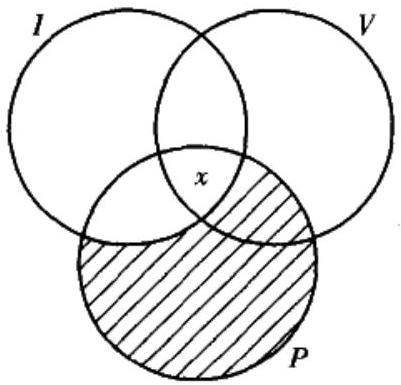
\includegraphics[max width=\textwidth, center]{2025_05_15_6a28331d5e7c993ad07ag-307}

2.有的金属是稀有而珍贵的物质,没有焊工的工具是非金属,所以,有的焊工的工具是稀有而珍贵的物质。

3.有亚洲国家不好战,因为所有好战国家是英国或者德国的盟友,而有亚洲国家并不是英国或德国的盟友。

4.有不酗酒的人是运动员,因为没有酗酒的人是身体素质好的人,而有的身体素质好的人不是非运动员。\\
*5.所有易燃物(inflammable)是不安全的东西,所以,所有安全的东西是非爆炸物,因为所有爆炸物是容易点燃的东西(flammable)。

6.世间所有物品都是可交换物,因为世间没有什么物品是非物质的东西,而没有物质的东西是不可交换物。

7.所有那些既非会员又非会员的客人的人都要被排除,因此,没有非国教徒(nonconformists)是会员或会员的客人,因为包括在其中的人都是国教教徒。

8.所有会死之物都是不完美的存在,没有人是不死的,所以,所有完美的存在都是非人。

9.所有在场的东西都是非刺激物(nonirritants),所以,没有刺激物 (irritants)是不可觉察的,因为所有可觉察的都不在场。\\
*10.所有有用的东西是不超过 6 英尺的,因为所有难以储存的东西是无用的,并且没有超过 6 英尺的东西是容易储存的。

\section*{7.3 直言命题的标准化}
如 7.1 节所述,日常语言中三段论论证的形式可能偏离标准形式,不仅可能出现含有三个以上词项的情况(如 7.2 节讨论的那样),还可能有

这样的情况,即构成命题不都是标准的直言命题。显然,A、E、I、O命题有些生硬,而日常生活中许多三段论都是由非标准的命题组成的。要把这些论证化归为标准形式,就要把构成命题都翻译为标准形式。但日常语言内容丰富、形式多样,根本无法找出一套完善的翻译规则。在各种情形中,最关键的是理解已知的非标准命题的含义,这样才能在翻译时不丢失,也不改变原意。

尽管没有完善的规则,我们仍然可以介绍一些方便的方法,它们在处理某些特殊命题时常常十分有用。这些方法——本节介绍九种方法——只能被看做一种指针而不是规则,也就是说,它们是处理某些特定种类的非标准命题的技巧。

1.单称命题。有些命题肯定或否定的是一个特定的个体或对象属于某个类,例如"苏格拉底是哲学家"、"这张桌子不是古董"等。这样的命题叫做单称命题。它们肯定或否定的不是一个类与另一个类的包含关系 (像标准式直言命题那样),但我们可以把单称命题解释为处理类与类间关系的命题。可以按如下方式做到这一点:

每一个个体对象都对应着一个单元类(由一个元素组成的类),其中只有一个对象。这样,断定一个对象 $s$ 属于类 $P$ ,在逻辑上等价于断定了只含有一个元素的单元集 $S$ 完全包含于类 $P$ 之中。而断定一个对象 $s$ 不属于类 $P$ ,在逻辑上等价于断定只含有一个元素的单元类 $S$ 完全排斥在类 $P$之外。通常将这种解释看做自然而然的,无须调整记法。据此,我们就可以将任何一个单称肯定命题"$s$ 是 $P$"看做逻辑上等价的 A 命题"所有 $S$是 $P$"。同样,可以简单地将单称否定命题"$s$ 不是 $P$"看做逻辑上等价的 E 命题"没有 $S$ 是 $P$"——S 指称的都是只有一个对象 $s$ 的单元类。因此,不需要对单称命题进行明确的翻译,一般把它们分别归到 $\mathrm{A} 、 \mathrm{E}$ 命题当中。康德说过"在三段论中判断之使用,逻辑学者把单称判断类如全称判断处理,是很恰当的"${ }^{[1]}$ 。

然而,情况并不那么简单。特称命题有存在含义,而全称命题没有。在布尔解释下(如5.6节说明),如果机械地把单称命题当做三段论推理的 A、E 命题;再用文恩图或三段论规则来检验其有效性,就会出现严重的困难。

很明显,在某些情况中,可以把含单称命题的有效的两前提论证转化为有效的三段论。例如:

$$
\begin{array}{ll}
\text { 所有 } H \text { 是 } M, & \text { 可以变为三段论的 Barba- } \\
\frac{s \text { 是 } H,}{\therefore s \text { 是 } M_{0}} & \text { ra, 即 AAA-1 式, 很明显 } \\
\text { 是有效的 } &
\end{array}
$$

$$
\begin{aligned}
& \text { 所有 } H \text { 是 } M, \\
& \text { 所有 } S \text { 是 } H, \\
& \therefore \text { 所有 } S \text { 是 } M \text { 。 }
\end{aligned}
$$

但在另外的某些情形下,把含单称命题的有效的两前提论证转化为三段论,却是明显无效的。例如:

$$
\begin{array}{ll}
s \text { 是 } M, & \text { 得到的直言三段论是无效 } \\
\frac{s \text { 是 } H,}{\therefore \text { 有 } H \text { 是 } M_{0}} & \text { 的 AAI-3 式 }
\end{array}
$$

后者违反了规则 6 ,犯了存在谬误。\\
再者,如果把单称命题转化为特称命题,也会有同样的困难。有些情况下转化是有效的,例如:

\begin{center}
\begin{tabular}{lll}
所有 $H$ 是 $M$, & 可以变为三段论的 Darii, & 所有 $H$ 是 $M$, \\
$\frac{s \text { 是 } H,}{\therefore s \text { 是 } M \text { 。 }}$ & 即 AII-1 式,很明显是有效的 & 有 $S$ 是 $H$, \\
$\therefore$ 有 $S$ 是 $M$ 。 &  &  \\
\end{tabular}
\end{center}

但在另一些情况中,这种翻译却会得出明显无效的直言三段论。例如:

\begin{center}
\begin{tabular}{lll}
$s$ 是 $M$, & 得到的直言三段论是无效的 & 有 $S$ 是 $M$, \\
$\frac{s \text { 是 } H,}{\therefore}$ 有 $H$ 是 $M$ 。 & 有 $S$ 是 $H$, &  \\
$\therefore$ & 有 $H$ 是 $M$ 。 &  \\
\end{tabular}
\end{center}

后者违反了规则 2 ,犯了中项不周延谬误。\\
问题来自如下事实:单称命题要比任何一个标准式命题负载更多信息。如果把"$s$ 是 $P$"当做"所有 $S$ 是 $P$",那么,就丢掉了单称命题的存在含义,实际上这里 $S$ 非空。而如果把"$s$ 是 $P$"当做"有 $S$ 是 $P$",又漏掉了单称命题的全称性,即主项周延,它说的是全部 $S$ 是 $P$ 。

解决此问题的办法,就是把单称命题分析为两个直言命题的合取,即

一个单称肯定命题等价于相互关联着的 A、I 命题的合取。这样"$s$ 是 $P$"就等价于"所有 $S$ 是 $P$"合取"有 $S$ 是 $P$",单称否定命题则等价于"没有 $S$ 是 $P$"合取"有 $S$ 不是 $P$"。图7—1就是单称命题的肯定式和否定式的文恩图。在用三段论规则评估这种推理时,必须考虑它提供的所有信息,既考虑周延性也考虑存在含义。\\
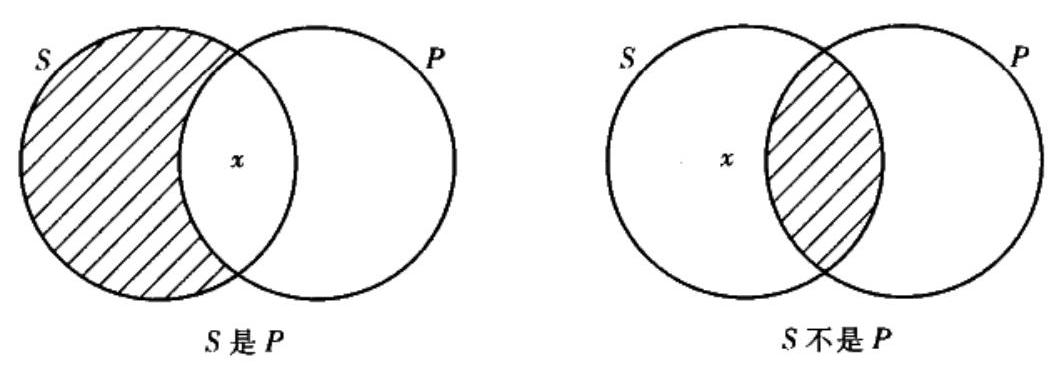
\includegraphics[max width=\textwidth, center]{2025_05_15_6a28331d5e7c993ad07ag-310}

图7—1\\
对于含有单称命题的三段论,引用文恩图或规则检验其有效性时,只要我们记住其中有存在含义,就可以直接把它们看做全称(A 或 E )命题。

2.谓项为形容词或形容词短语,而非名词或类词项的直言命题。例如"有花是美的"、"没有战船是可调用的"都是直言命题,但"美的"和 "可调用的"表示的只是属性而不是类,所以它们的形式不标准,必须转化为标准形式。不过,每个属性都可以确定一个类,即具有这种属性的事物组成的类,所以对于每个这样的命题,都有一个相应的标准式直言命题。两个例句分别对应的是:I命题"有花是美的事物"和 E 命题"没有战船是可调用的事物"。如果一个直言命题的形式是标准的,只有谓项为形容词或形容词短语时,就把形容词或短语替换为这样一个词项,它指称由所有具有形容词表示之属性的事物所组成的类。

3.主要动词不是标准的联项"是"或"不是"的直言命题。常见的例子有"所有人都寻求赞誉"、"有人饮用希腊酒"。通常,转化的方法是把主项和量项之外的所有成分看做类的定义特征。先把能被替换的成分换成这样的词项,它们指称由类定义特征所确定的类,再改用标准的联项把它们同主项联结起来。这样上面两个例子就成了:"所有人是赞誉的寻求者"、"有人是希腊酒的饮用者"。

4.标准形式的各成分都出现,却没有按标准顺序排列的陈述句。"赛马全是良种马"和"结果好的事总是好事"就是这样的例子。在这种情形

下,首先要找出哪个是主项,然后再重新把各个成分排列一下,使之成为标准式直言命题。这种翻译通常都很直接。十分清楚,上述两个例句可翻译为"所有赛马是良种马"和"所有结果好的事是好事"。

5.量词不是"所有"、"没有"和"有"这些标准语词的直言命题。以 "每一"、"任何"等开头的陈述句很好转化。"每一只狗都有其得意之时"、 "任何贡献都会得到赞赏"可分别转化为"所有狗是有其得意之时的动物"和"所有贡献是会得到赞赏的事情"。"每一事物"、"任何东西"类似于 "每一"、"任一"。与此同一系列但限于人类的是"每人"、"任何人"、"无论谁"、"不管是谁"、"那些……的人"以及"每个......的人"等等。以上各表达式都不会带来什么麻烦。

语法冠词"a"和"an"("一个"等)也可用于指代量词,必须依据当时的语境,确定它们的意思是"所有"还是"有"。例如,"A bat is a mammal"(一只蝙蝠是一个哺乳动物)与"An elephant is a pachyderm" (一头大象是一个厚皮动物)可以合理地解释为"所有蝙蝠都是哺乳动物"与"所有大象都是厚皮动物"。但"A bat flew in the window"(一只蝙蝠飞进窗户)和"An elephant escaped"(一头大象逃跑了)显然指的是 "有蝙蝠是飞进窗户的动物"和"有大象是逃跑的动物"。

冠词"the"("这"、"这些"等)既可以用于指称一个特定的个体,也可以指称一个类的全部元素,有可能引起混淆。例如"The whale is a mammal"(鲸是哺乳动物)这句话,在一般情况下都会被理解为"所有鲸都是哺乳动物",而单称命题"The first president was a military hero" (第一任总统是军旅英雄)可以说是标准形式的 A 命题(一个有存在含义的单称命题),其道理本节前面已经讨论过了。 ${ }^{[2]}$

尽管以"每一"和"任一"开头的肯定句都可以译为"所有 $S$ 是 $P$",但对于以"not every"(并非每一个)和"not any"(并非任一)开头的否定句,却有很大区别。它们的译法不那么明确,需要更加小心。比如, "Not every $S$ is $P$"意思是有 $S$ 不是 $P$ ,而"Not any $S$ is $P$"意思是没有 $S$ 是 $P$ 。

6.排斥命题(exclusive propositions)。含有"只"(only)、"只有" (none but)的直言命题通常叫做排斥命题,因为一般说来,它们断言的是谓项排他性地适用于主项。例如"只有公民能成为选民"、"只有勇敢者是值得公平对待的",第一句转化为标准形式是"所有能成为选民的是公

民",第二句转化为"所有值得公平对待的人是勇敢者"。以"只"、"只有"开头的命题一般可以按以下途径转化为 A 命题:将主、谓项互换位置,把"只有"换为"所有"。因此"只有 $S$ 是 $P$"和"只有 $S$'s 是 $P$'$s$"通常被理解为"所有 $P$ 是 $S$"。

但是,在某些语境中,"只"、"只有"被用于表达某种更多的含义。 "只有 $S$ 是 $P$"和"只有 $S$'s 是 $P$'$s$"表明的可能是"所有 $S$ 是 $P$"或者 "有 $S$ 是 $P$"。但这种情况并不常见。这个时候就需要语境的辅助了。如果没有附加信息,前面的翻译就是适当的。

7.不含量词的直言命题。例如"狗是肉食动物"、"孩子在场"。欠缺量词,句子的含义就不十分明确。只有考察它们所处的语境才能确定其含义,一般来说,考察之后就能把疑义清理掉。第一个例句"狗是肉食动物"很可能述及了所有的狗,可以转化为"所有狗都是肉食动物"。而第二个例句一般只述及某些孩子,转化为标准形式为"有孩子是在场的人"。

8.完全不像标准式直言命题但也可以有标准式翻版的命题。例如 "不是所有孩子都相信圣诞老人"、"有白色的大象"、"没有粉色的大象"以及"没有既圆又方的东西"。反思这些命题就会发现,它们在逻辑上等价于(因而可翻译为)下面的标准式命题:"有孩子不是相信圣诞老人的人"、"有大象是白色的事物"、"没有大象是粉色的事物"和"没有圆的东西是方的"。

9.除外命题(exceptive propositions)。还有一些这样的例子:"除了雇员(all except)都是合格的"、"雇员之外的人(all but)都是合格的"与"只有(alone)雇员不是合格的"。要把这样的除外命题翻译为标准形式,情况就会复杂一些,因为这种命题(与单称命题很类似)做出了两个而不是一个方面的断定。所给例子断言的不仅是所有非雇员是合格的,还断定了(在通常的语境中)没有雇员是合格的。如果把"雇员"记为 $S$ 、 "合格的人"记为 $P$ ,那么,这两个命题可以写成"所有非 $S$ 是 $P$"和 "没有 $S$ 是 $P$"。这两个命题是独立的,但联合起来就断定了 $S$ 和 $P$ 互为补类。

每个除外命题都是复合句,因此,不能转化为单一的标准式直言命题。确切地说,每一个除外命题应当翻译为一个合取式,即两个标准式直言命题的合取式。所以,上面关于合格性的三个例句都可以翻译为"所有非雇员是合格者,并且没有雇员是合格者"。

应该注意到,有些论证的有效性离不开数字或类数字(quasi-numeri- cal),但数字无法译为标准形式。这些推理本身就是非三段论的(asyllo- gistic)。因此,对它们进行分析就需要一种比直言三段论复杂一些的理论。当然,有些含有类数字量词的推理也可以用三段论分析。"几乎所有"、"并非全部"、"除少数几个之外都"、"几乎每个人"等就是这样的词。如果一个命题含有看起来像量词的词项,那么就可以处理为刚刚讲过的除外命题。下面几个除外命题都含有类数字:"几乎所有学生都参加了舞会"、"并非所有学生都参加了舞会"、"除少数几个之外,学生们都参加了舞会"和"只有一些学生参加了舞会",它们都肯定了有些学生参加了舞会,同时又否定了所有学生都参加了舞会。从三段论推论的观点看,它们给出的类数字信息并不相干,转化之后都是"有学生是参加了舞会的人,并且有学生不是参加了舞会的人"。

由于除外命题不是直言命题,而是合取式,含有这些命题的论证并不是我们所说的三段论论证。但是,对它们进行三段论分析和评估也未尝不可。含有除外命题的论证,要依据该命题所处的位置来进行检验。如果它是前提,那么就要分两次进行检验。举例来说,看下面这个论证:

\begin{displayquote}
每个看过比赛的人都参加了舞会,\\
不是全体学生都参加了舞会,\\
所以,有学生没有看过比赛。
\end{displayquote}

其中,第一个前提以及结论都是直言命题,很容易译为标准形式。但第二个前提是一个除外命题,不是简单句而是复合句。要检查前提是否蕴涵结论,首先要检验由论证的第一个前提、第二个前提的前一半以及结论组成的三段论。我们有:

\begin{displayquote}
所有看过比赛的人都是参加了舞会的人,\\
有学生是参加了舞会的人,\\
所以,有学生不是看过比赛的人。
\end{displayquote}

这个标准式的直言三段论是 AIO-2,违反了规则 2,犯了中项不周延的谬

误。但不能由此就得出结论说原来的论证是无效的,因为受检验的三段论只包含它的一部分前提。现在再来检验由第一个前提、第二个前提的后一半以及结论组成的三段论。译为标准形式后,得到一个非常不同的三段论:

所有看过比赛的人都是参加了舞会的人,\\
有学生不是参加了舞会的人,\\
所以,有学生不是看过比赛的人。

这是一个标准的 Baroko,即三段论的 AOO-2。很容易看出它是有效的。原来的三段论与这个有效式的结论相同,并且前者的前提包含着后者的前提,所以原来的论证也是有效的。因此,如果一个论证中有一个前提是除外命题,那么,对其有效性的检验要分为两次,即分别对两个不同的标准式直言三段论进行检验。

如果前提都是直言命题,但结论是除外命题,那么我们就可断言它是无效的。尽管两个直言命题可以蕴涵其中一个,即蕴涵结论复合句的一半,但不可能同时蕴涵两个。最后,如果两个前提和结论都是除外命题的话,那么,由原来论证所能建构的任何一个可能的三段论都要接受检验,才能确定其有效性。以上解释已足够处理这种情况了。

学会将多种非标准命题翻译为标准形式的技巧是很重要的,因为我们已经掌握的检验方法——文恩图解和三段论规则——只能直接用于标准式直言三段论。

\section*{练习题}
将下列各题翻译为标准式直言命题。

\section*{例题}
1.玫瑰花有香味。\\
翻译后标准形式为:所有玫瑰花是有香味的东西。\\
2.洋葱没有香味。\\
3.许多人都后悔年轻时虚度了光阴。\\
4.不是每个值得一见的人都是值得当做朋友的人。\\
*5.如果这是一个 Junko,它就是钱能买到的最好的东西。\\
6.如果它不是真的哈瓦那(Havana)雪茄,就不是罗泊(Ropo)牌的。

7.没有既安全又刺激的东西。\\
8.只有勇敢者才能获得国会荣誉勋章。\\
9.忠言逆耳。\\
*10.面朝太阳的人看不到自己的影子。\\
11.听她唱歌令人精神振奋。\\
12.玩火者自焚。\\
13.只有会员可以人内。\\
14.没人不喜欢萨拉•李(Sara Lee)。\\
*15.土耳其青年都不拥护护卫军候选人。\\
16.款式都不错,除了那些令人厌倦的。\\
17.他们也为那些只能站着等待的人服务。\\
18.知足者常乐。\\
19.美的事物是永恒的喜悦。\\
*20.博爱者皆虔诚。\\
21.闪闪发光者不都是金子。\\
22.只有伟人才思考大痛苦。\\
23.嘲笑伤疤的人没受过伤。\\
24.种瓜得瓜,种豆得豆。\\
*25.灵活的答案可以避免非议。

\section*{7.4 协同翻译}
要对三段论论证进行有效性检验,其中总共只能包含三个项。有时做到这一点很难,需要比前面所述方法更细致的处理。请考虑命题"你总是与穷人为伍",显然,它既不是断言所有穷人总是在你身边,也不是说有些(特称的)穷人总是(always)在你身边。把该命题化归为标准形式的一种方法,也是一种最自然的方法,就是从其中的关键词"总是"着手分析。这个词意味着"在所有时间"(at all time),它表明原命题的一种标准式翻版为"所有时间都是你与穷人为伍的时间"。主、谓项中都出现的\\
"时间"这个词可视为一个参项(parameter)。所谓参项,就是一个有助于以标准形式表达原来断言的辅助词项。

当然,绝不能机械地、不加思考地引入和使用参项,必须始终以所要翻译的那个命题为依据。命题"史密斯总是在台球比赛中获胜",显然断定的并不是史密斯从不间断地、始终在获胜!较合理的解释是,这句话是说:每当史密斯玩台球时,他就会获胜。如果这么理解,就可以直接把原句转化为"所有史密斯玩台球的时间是他获胜的时间"。并非所有参项都是时间性的。在对另一些命题进行翻译时,"地点"(place)、"情形"(case)也能被用做参项。例如"没有幻想的地方人类就会毁灭"(Where there is no vi- sion the people perish)和"每当琼斯迟到就丢失一次推销机会"(Jones lo- ses the sale whenever he is late)可分别译为:"所有没有幻想的地方都是人类毁灭的地方"和"所有琼斯迟到的情形都是他丢失推销机会的情形"。

在对三段论的三个构成命题进行协同翻译的过程中,参项的引人是必不可少的。一个直言三段论恰好包含三个项,要检验三段论就必须把它的构成命题都转化为标准式直言命题,其中只出现三个项。去除同义词以及换位法、换质法、换质位法的运用已经在 7.2 节讨论过。即使这样,还有很多三段论论证的项数仍然不能被缩减到三。此时,协同翻译就需要把同一个参项引到三个构成命题中去。请看下面这个论证:

\begin{displayquote}
哪里脏纸盒散落哪里就曾有不自爱者在此野餐,这里散落着脏纸盒,
\end{displayquote}

所以,一定有不自爱者在这里野餐过。

这个推理是完全有效的,但只有把前提和结论都翻译为标准式直言命题,并且其中只能有三个项,才能用文恩图或三段论规则来证明其有效性。第二个前提和结论能很自然地译为"有脏纸盒是散落在这里的东西"和"有不自爱者是在这里野餐过的人"。但这两个陈述句当中有四个不同的项。要把给定的论证化归为标准形式,就需要在三个命题中使用同一个参项。我们从第一个前提着手寻找这个参项,然后再用同样的参项去翻译第二个前提以及结论。"哪里"一词表明可以用"地方"作为参项。如果翻译三个命题时都用这个参项,则论证可变为:

所有散落脏纸盒的地方是不自爱者野餐过的地方,这个地方是散落脏纸盒的地方,所以,这个地方是不自爱者野餐过的地方。

这个标准式直言三段论的形式为 AAA-1,即 Barbara,是一个已经被证明有效的形式。

利用参项使表达式标准化的方法不是很容易掌握的,但有些三段论论证的确无法用其他方法进行翻译。再看一个例子有助于弄清其中的技巧:

每当狐狸经过那里,猎犬一定会发出叫声,所以,狐狸走的一定是别的路,因为猎犬都很安静。

首先,我们必须明白上述论证说的是什么。要把"猎犬很安静"这句话理解为"猎犬此时此地没有发出叫声"。这一步是去除同义词的必需步骤,因为第一个命题说的是"猎犬发出叫声"。同样,"狐狸走的一定是别的路"的结论,应理解为断言"狐狸没有经过那里"。第一个前提中的"那里"一词表明翻译时也可用"地方"做参项。于是,可得到这样一个标准式翻版:

$$
\begin{aligned}
& \text { 所有狐狸经过的地方是猎犬发出叫声的地方, } \\
& \text { 这个地方不是猎犬发出叫声的地方, } \\
& \text { 所以, 这个地方不是狐狸经过的地方。 }
\end{aligned}
$$

这个标准式直言三段论的形式为 AEE-2,即 Camestres,其有效性很容易确定。

\section*{练习题}
I.使用恰当的参项,将下列命题翻译为标准形式。

\section*{例题}
1.一提起他的损失他就叹息不已。

\section*{解答}
此命题可译为标准形式:所有提起他的损失的时候都是他叹息不已的时候。\\
2.她从不开车上班。\\
3.他总是走自己选择的路。\\
4.他总是点菜单上最贵的菜。\\
*5.除非问她,否则她从不发表意见。\\
6.她到处兜售人寿保险。\\
7.他一生气就脸红。\\
8.只要请他讲几句,他就能聊半天。\\
9.哪里有对错误意见的宽容,哪里才有自由争论。\\
${ }^{*} 10$ .人们对问题的正确决断从来不会在自由争论时做出。\\
II.将下列论证:\\
a.翻译为标准式;\\
b.指出相应标准式的式与格;\\
c.用文恩图检验其有效性,如果是有效式,请指出其名称;\\
d.如果是无效式,指出其中所犯的谬误。

\section*{例题}
1.所有知识都来自感觉印象,由于不存在实体自身的感觉印象,于是可以逻辑地推出:没有关于实体的知识。\\
-Robert M.Pirsig,Zen and the Art of Mo- torcycle Maintenance

\section*{解答}
a.标准式为:\\
没有来自感觉印象的东西是关于实体自身的知识,所有知识是来自感觉印象的东西,\\
所以,没有知识是关于实体自身的知识。\\
b.式与格:EAE-1\\
c.有效,Celarent。文恩图如下:\\
2. $\qquad$对立偶中没有名称,但所有范畴都在对立偶中,所以,没有名称是范畴。\\
--Peter Thomas Geach,Reference and Gener-

3.每个吸食鸦片的人都会尝试海洛因,每个尝试海洛因的人都会不可救药地上瘾,所以,每个吸食鸦片的人都会不可救药地上瘾。

4.对于天体而言,如果一个处于它之上的自由摆动、长度固定的钟摆,其振动周期随纬度的增加而逐渐减小,那么,它一定是椭圆形的,从赤道至两极逐渐变得扁平。

而地球就是这样一个天体,一个处于它之上的自由摆动、长度固定的钟摆,其振动周期随纬度的增加而逐渐减小。

所以,地球一定是椭圆形的,从赤道至两极逐渐变得扁平。\\
-W.A.Wallace,Einstein,Galileo,and Aquinas:Three Views of Scientific Method\\
*5.巴塞罗那运输公司(Barcelona Traction)负担不起债务利息,破产的公司都负担不起债务利息,所以,巴塞罗那运输公司必定是破产公司。\\
--John Brooks,"Annals of Finance",The New Yorker, 28 May 1979\\
6.无论在自由、美德或其他什么问题上持极端主义总是一种恶行一一因为极端主义就是狂信的另一种说法,而狂信的应有之义就是一种恶行。\\
--Irving Kristol,"The Environmentalist Crusade",Wall Street Journal, 16 De- cember 1974

7.当教师的价值观与社会规范冲突时,特别是与地方社区、行政人员、学生或者其他教师的标准冲突时,其职业生涯将充满紧张气氛。

当今的社会是多元化的,至少从原则上讲,它有助于尊重个性差异、有助于全民教育普及。教师的价值观不可避免地与他们所在的社区的某个或某些部分发生冲突。因此,紧张气氛就是当今公共教育职业生涯中的必然状况。\\
----David W.Adams,"Tired and Frustrated Teachers",Today's Education,January 1975\\
8.所有含有两个否定前提的三段论都是无效式。有些有效的三段论是可靠的。所以,有些不可靠的论证是含有两个否定前提的三段论。

9.如果两个人说出的话互为矛盾,他们不可能都在说谎。因此第一个土著人和第三个土著人不可能都在说谎,因为他们说的话互为矛盾。\\
*10.不是所有发光的都是金子,因为贱金属(base metal)发光,而金子不是贱金属。

11.经常喝醉的人都是靠不住的,所以,所有可靠的人都是非酗酒者,因为所有酗酒者经常喝醉。

12.冒烟处就是着火处,所以,地下室没着火,因为那里没冒烟。\\
13.似乎上帝并不怜悯(mercy),大马士革人(Damascene)认为,怜悯是一种遗憾(sorrow),而上帝并没有遗憾,所以说,上帝并不怜悯。\\
-Thomas Aquinas,Summa Theologiae,I, question 21,art. 3\\
14.$\cdots \cdots$ 因为狂热不是别的,而是一种痛苦的感情,痛苦不在别处存在,只有有感知的人才会有。由此可知,没有狂热可以真正在无感知肉体内存在。\\
---George Berkeley,Three Dialogues be- tween Hylas and Philonous,in Opposi- tion to Skeptics and Atheists\\
*15.只有那些不顾事实的人会犯错误,没有真正客观的人会犯错误。因此没有不顾事实的人是真正客观的。

16.所有打桥牌的都是人。所有人会思考。因此所有打桥牌的都会思考。\\
——Oswald and James Jacoby,"Jacoby on Bridge",Syndicated Column, 5 Novem-

17.每当我陷人困境就会祈祷。因为我总是陷在困境中,所以,我没有一天不祈祷。\\
-Isaac Bashevis Singer,interview in the New York Times\\
18.余像不存在于我们生活的物理空间中,而脑运动则存在其中。所以余像不是一种脑运动。\\
--J.J.C.Smart,"Sensations and Brain Processes",Philosophical Review,April 1959

19.刚刚肯定下过雨,因为鱼不咬钩,雨后的鱼从不咬钩。\\
*20.……显然无理数对工程师没什么意义,因为他们只关注近似值,而所有近似值都是有理数。\\
-G.H.Hardy,A Mathematician's Apology\\
21.所有实践都是学问,外科是实践,由是可知,所有外科是学问。\\
——Lanfranc,Chirurgia Magna\\
22.因为与邻邦作战是恶行,而与底比利斯作战就是与邻邦作战,所以很显然,与底比利斯作战就是恶行。\\
---Aristotle,Prior Analytics\\
23.根据亚里士多德的说法,没有自然现象源于偶然。他的论据是:源于偶然的东西不能一直出现或者经常重现,但是所有自然现象或者一直出现或者经常重现。\\
-Moses Maimonides,The Guide for the Perplexed\\
24.她告诉我,她对学生的态度很简单,事实上,如同她对一般人一样。也就是说,她一生只与出身高贵的夫人和绅士谈话。既然众多学生中没有这样的人,她就不,从来不,也不可能与学生谈话。\\
--James Herndon,The Way It Spozed to Be\\
*25.不是所有有工作的人都能节制饮酒量。只有负债人才酗酒。所以并非所有失业者都负债。

26.明天一定有好戏看,因为会议主题极为敏感,没有敏感主题的争论是乏味无趣的。

27.比尔今天上午没有上班,因为他穿了一件运动衫,他从不穿运动衫上班的。

28.辛西娅一定夸奖亨利了,因为亨利现在很兴奋,辛西娅每次夸奖他,他都很兴奋。

29.每个见到爱丽丝的男孩子都会喜欢她,而每个与贝蒂约会的男孩子都会见到爱丽丝,所以每个与贝蒂约会的男孩子都会喜欢爱丽丝。\\
*30.这个工厂一定在罢工,因为那里有一队纠察员,只有罢工时才会有纠察员。

31.流行病学者往往这样说,流行病学不仅仅研究传染病的流行,而是广泛考察人群中疾病(disease)的流传方式和速度。滥用任何良药都可以看做一种病态(disease),因此,流行病学方法对此项研究是有益的。\\
$\qquad$ "Science and the Citizen",Scientific American,February 1975\\
32.不懂诗歌的人不能朗诵诗歌,因为朗诵者应该把诗的精神传达给听众,除非他懂得自己要表达的是什么,否则,他如何很好地表达自己呢?

\section*{-Plato,Ion}
33.道德原则既然对行为和感情有一种影响,所以当然的结果就是,这些准则不能由理性得来;这是因为单有理性永不能有任何这样的影响,这一点我们前面已经证明过了。\\
-David Hume,A Treatise of Human Na- ture

34.任何值得逻辑研究的论证形式必出现在日常话语中,我们发现三段论第四格在日常话语中并不出现,所以三段论第四格是不值得逻辑上研究的。\\
*35.所有有效的三段论中项至少在一个前提中周延,这个三段论一定有效,因为其中中项至少在一个前提中周延了。

36.只有特快列车不在这个站停靠,上一趟车没有停靠,所以那一定是特快列车。

37.有效三段论都不能包含两个否定的前提,本页的三段论都不是无效的,所以说,本页没有包含两个否定前提的三段论。

38.高民调支持率有助于筹集资金,好的新闻與论会使人得到高民调

支持率,所以说,好的新闻舆论有助于筹集资金。

\begin{displayquote}
an advisor to Elizabeth Dole, during her campaign for the Republican presidential nomination quoted in the New York Times, 15 April 2000
\end{displayquote}

39.此处有植物生长,因为草木生长需要水,所以,这里一定有水。\\
*40.出席的人没有失业者,没有会员缺席,因此所有会员都有工作。\\
41.这场竞争是激烈的,因为其中涉及大笔钱财,与钱财密切相关的竞争都不平静。

42.许多人很漂亮,但只有人类是丑恶的,所以如果说不存在既漂亮又丑恶的事物是错的。

43.同样,单纯的事物是不可再分的,灵魂是单纯事物,所以它是不可再分的。\\
--Dun Scotus,Oxford Commentary on the Sentences of Peter Lombard\\
44.不是所有发光的都是金子,所以金子不是唯一的贵金属,因为只有贵金属才发光。\\
*45.尽管他一生病就会怨天尤人,但他现在的身体很棒,所以他现在不会怨天尤人。

46.没有头脑清醒的证人会指控自己,但有些证人指控自己,所以有些证人是头脑不清醒的。

47.我们可以把一个形而上学句子规定为想去表达一个真命题的句子,但是事实上,它既不表达一个重言式,又不表达一个经验假设,并且因为重言式和经验假设构成有意义命题的整个类,所以我们就有理由下结论说,一切形而上学断定都是无意义的。\\
——Alfred J.Ayer,Language,Truth,and Logic\\
48.这个三段论有效,因为所有无效三段论都有不当步骤,而这个三段论中没有不当步骤。

49.所有穷人被宣判有罪,有些罪犯被开释。因此有些有钱人不是无罪的。\\
*50.所有高于 300 英尺的建筑都是摩天大楼,但并非所有现代建筑都

高于 300 英尺,因为并非只有摩天大楼是现代建筑。

\section*{7.5 省略三段论(Enthymemes)}
三段论论证很常用,但其前提和结论并不总是都得到明确地陈述。常常只把论证的一部分表述出来,而其余部分就要靠"领会"了。比如,只提及"琼斯是个土生土长的美国人"这个前提,就可以得到结论:"琼斯是美国公民"。上述论证的表述并不完整,但很容易根据美国宪法把省略的前提补出来。加上被省略了的前提,完整的论证就是:

\begin{displayquote}
所有土生土长的美国人是公民,\\
琼斯是土生土长的美国人,\\
所以,琼斯是美国公民。
\end{displayquote}

完整表述后,这个论证就是一个直言三段论,其形式为 AAA-1,即 Bar- bara,它完全有效。如果一个推理是不完整的,其中有一部分需要"领会"或仅仅"在心中",我们就称之为省略三段论。省略(enthymematic)是不完整三段论的特征。

在日常话语甚至科学中,许多推论都是省略式的。原因不难理解,因为有相当一部分命题是公共知识。对于那些广为人知或无关紧要的真命题,听众和读者很容易就能想到并且补充完整,说话者和写作者就不再重复以减少麻烦。另外,用省略式描述推理,能够增加修辞效果,比描述出所有细节更强、更有说服力。亚里士多德在其著作《修辞学》中写道: "基于省略三段论的……演讲更受人欢迎。"

由于省略式不完整,所以要检验其有效性必须找到被省略的部分。如果省去的是一个必不可少的前提,缺了它推论就是无效的。但是如果省略的前提很容易补出来,评估时应该把它包括在论证当中才是公平的。这时,要假定论证者心中所想比明确说出的信息更多些。大多数情况下,很容易将说话人(或写作者)想到而没有表达出来的前提补充完整。举例来说,要说明"银色马"的怪事,神探福尔摩斯构造了这样一个推论,其中就省略了关键性前提,但是很容易猜到:

马厩中有一条狗。然而,尽管有人进来,并且把马牵走,狗却没有出声……显然,来者是这只狗非常熟悉的人物。

我们都能很好地理解其中暗含的意思:如果来者是陌生人,狗就会发出叫声。把这个前提看做福尔摩斯论证的一部分,对作者柯南-道尔来说才是公平的。

补充隐藏的前提时最重要的原则是:说话人确实认为听者可以接受这个命题为真。因此,要是把结论本身当做隐藏的前提就太愚委了。如果论证者希望听者把它当做前提而不加证明,那就无须再作为论证的结论来表述。

任何论证都能以省略式表达,但得到最广泛研究的还是三段论的省略式,本节也只限于研究三段论的省略问题。根据未表述部分的不同,传统上把省略三段论分为几种不同的省略体。三段论的第一种省略体指不出现大前提的情形。上面的例子就是这种省略体。第二种省略体保留大前提和结论,而不出现小前提。例如"所有学生都是反对新规则的,所以,所有大二学生都是反对新规则的",这里的小前提是个明显为真很容易补充出的命题:"所有大二学生是学生"。第三种省略体中两个前提都出现,但未表述结论。下面就是这个类型的例子:

我们的观念超不出我们的经验:我们没有关于神圣的属性与\\
作为的经验:我们用不着为我这个三段论下结论:你自己能得出推论来。 ${ }^{[3]}$

检验省略三段论的有效性共需两步:首先恢复省略的部分,然后再检验。公正地表示出省去的命题,需要语境敏感性以及对说话者意图的理解。请看这样一个论证:"没有真正的基督徒是精神空虚的,但有些常去教堂礼拜的人是精神空虚的",其中没给出结论,属第三种省略体,那么,原本要得出的结论是什么呢?如果说话者是要得出"有些常去教堂的人不是真正的基督徒",那么,推理就是有效的(EIO-2,Festino);但是如果说话者想说的是"有些真正的基督徒不是常去教堂的人",那么,这个省略式就是无效的(IEO-2),犯了大项不当周延谬误。

但一般说来,语境可以无歧义地确定未表述的命题。例如根据最高法

院的意见,控制州内性暴力的联邦立法("针对妇女的暴力行为法案")是违反宪法的,大多数法官的关键性论证如下:

在任何意义上,性暴力犯罪都不是经济行为……迄今为止,在美国的历史上最高法院的判例中,只有经济行为才适用控制州内行为的条款。 ${ }^{[4]}$

可以领会但没有明确表述的结论是:根据最高法院的长期实行的规则,性暴力犯罪不归国会控制。

检验第三种省略体,先要把前提和(显而易见的)结论变形为标准形式。首先陈述大前提(含有结论之谓项的前提),然后确定其式与格,如上例:

大前提:根据最高法院的规则,国会控制的所有行为是经济行为。

小前提:没有州内的性暴力犯罪是经济行为。\\
结论(并未表述但结合语境却很清楚):没有州内的性暴力犯罪是最高法院规定为国会控制的。

这个三段论的式为AEE,中项在两个前提中都做谓项,因此是第二个格,其形式是 Camestres——有效的三段论。

第三种省略体,在某些情况下,即使不结合语境也能看出是无效的——例如,两个前提都是否定的,或者都是特称的,或者中项不周延。如果这样的话,不可能得出有效的结论。因此,这种省略式在任何语境中都是无效的。

也可能有这样的情况,在省略的是论证的一个前提的情况下,只有加上一个高度不合理的前提,才能把论证写成有效式。此时,指出这一点就构成对省略三段论的一种合理批判(legitimate criticism)。当然,更具毁灭性的批判是:有些三段论无论补上什么样的前提(即使是不合理的前提),也不能成为有效的三段论。

省略三段论与普通三段论的区别,从本质上说是修辞上的,而不是逻辑上的。不需添加什么新规则就能处理省略式,它们终究要接受与标准直

言三段论同样的检验。

\section*{练习题}
按如下要求处理下列省略式论证:\\
(a)给出一个被省去的合理的前提或结论;\\
(b)把论证写为标准形式,包括省去的前提或结论,如果可能的话,使论证成为有效式——必要时可使用参项;\\
(c)指出是哪种省略式;\\
(d)如果补全后的论证是无效式,指出其犯了哪种谬误。

\section*{例题}
1.转基因动物是人造物,因而是可申请专利的。\\
--Alan E.Smith,cited in Genetic Engineering (San Diego:Greenhaven Press,1990)

\section*{解答}
(a)被省略的前提是:人造物都是可申请专利的。\\
(b)标准形式为:\\
所有人造物都是可申请专利的东西,\\
所有转基因动物都是人造物,\\
所以,所有转基因动物都是可申请专利的东西。\\
(c)这是第一种省略体,因为省去的是论证的大前提。\\
(d)它是有效的论证,形式为 AAA-1,即 Barbara。\\
2.一切灵魂是不朽的,因为凡是永远处于运动之中的事物都是不朽的。

\section*{-Plato,Phaedrus}
3.亚伯拉罕-比莫 $\cdots \cdots$ 竞选市长的口号是——近几周频繁提到,但他没料到会这么具有讽刺性——"如果不懂得赚钱(buck)${ }^{(1)}$ ,就不懂得这项工作——但亚伯懂得赚钱。"\\
-The New Yorker, 26 August 1974\\
4.尽管这些课本号称价值很高的重要知识的通用指南,但有一个事

\footnotetext{(1)buck,多义词,在美国俚语中有"美元"、"公羊"、"吹牛"、"花花公子"等义。
}实与之相悖,在我六年的教师生涯中,无论是在乡村还是城市,没有一个人偷过课本。\\
----W.Ron Jones,Changing Education,Winter 1974\\
*5.事实上,像女人一样,男人也是肉身,因而也是被动的,是荷尔蒙与性征的玩弄对象、无休止欲望的牺牲品。\\
--Simone De Beauvoir,The Second Sex\\
6.你不会不尊重一个凶狠的对手,而且也不会痛恨一个你所尊重 278的人。\\
--Pancho Gonzalez,former U.S.Tennis Champion

7.……我是个唯心主义者,因为我相信所有存在都是精神性的。\\
——John McTaggart Ellis McTaggart,Philo- sophical Studies

8.为什么不能做一个彻底的神人相似论者?为什么不承认众神有肉体,也有眼、鼻、口、耳等等呢?伊壁鸠鲁曾坚持说,除了在人的形体中,没有发现过理性;因此,神必定具有人形。而这个曾经西塞罗正当地加以嘲弄的论证,依照你的说法,又变成可靠的、合乎哲理的论证了。\\
--David Hume,Dialogues Concerning Nat- ural Religion,Part V

9.但是曼彻斯特的书的合法性是经过法庭确认的,因此不是可以讨论的话题。\\
--A.L.Fain,"The Legal Right to Privacy", Saturday Review, 21 January 1967\\
*10.我不认为我们能拥有真正哲学意义上的自由,因为我们的行为不仅受外部压力的控制,而且还受内在需要的制约。\\
-_Albert Einstein\\
11.所有执业医生是大学毕业生,所以,所有美国医学协会的会员一定是大学毕业生。

12.小国能更好地铭记历史,因为历史往往对它们不利。\\
——Marc Falcoff,"Semper Fidel",The New

13.刚才一定下过雨,因为鱼现在不咬钩。\\
14.约德•卡休斯瘦骨嶙峋、一副饿相……这样的人很危险。\\
-William Shakespeare,Julius Caesar, act1,sc. 2\\
*15.亨利只想挣钱,但是一个人不能同时为上帝与金钱卖命!\\
16.亚当森一家没装电话,因为电话簿里没有他们的名字。\\
17.没有省略式是完整的,所以这个论证是不完整的。\\
18.他不愿接受王冠,因此他一定没有野心。\\
-William Shakespeare,Julius Caesar, act1,sc. 2

19.任何能把这个论证补全的学生都是优等生,因为,补全这个论证很不容易。\\
*20.他了解自己的孩子,所以他一定是个明智的父亲。\\
21. $\qquad$我们拥有一些无形的知识,但没有感官知识是无形的。\\
-Duns Scotus,Oxford Commentary on the Sentences of Peter Lombard

22.很难否认加在自由训练上的特别税法规是违反宪法的,而执照税就是这种法规的内容之一。\\
— Justice William O.Douglas,for the Court,Murdock v.Commonwealth of Pennsylvania, 319 U.S.105, 1943\\
23.请无罪的人投第一块石头吧。 ${ }^{(1)}$ 我敢肯定在座的每个人都有不可告人的丑事,而且我也能说出每个人的丑事。\\
-Representative Adam Clayton Powell,speech in the U.S.House of Representatives, 1967\\
24.只有证据才能让人放弃创世论,但自然界中没有这样的证据。\\
-Moses Maimonides,The Guide for the Perplexed\\
*25.毁灭性最弱的核武器可能最危险,因为,它们使核战争成为很容

\footnotetext{(1)此语出自《圣经•约輸福音》 $7: 8$ ,系耶稣对要求乱石处死一个淫妇的众人所说,结果众人听后悉数离去。现常用来表示"人人皆有罪"之意。
}易的事。\\
-Freemen Dyson,"Reflections:Weapons and Hope",The New Yorker, 6 February 1984\\
26.人类自身增长的速度有高于其生存能力增长速度的趋向,因此,随时会面临严峻的生存考验。\\
-Charles Darwin,The Descent of Man\\
27.没有内燃机无污染,而没有内燃机是全效的。这样,你自己就可以得出结论了。

28.没有道义观念的国家是没有灵魂的国家。没有灵魂的国家是不能生存的国家。\\
—Winston Churchill\\
29.自由意味着责任,这就是大多数人畏惧自由的原因。\\
--George Bernard Shaw,Maxims for Revo- lutionists\\
*30.假装有一些自己实际上没有的动机和能力,或假装自己的动机达到了实际上并不具有的强度,以及假装自己的能力达到了实际上并不具有的水平,这总是可能的。假如没有可能做出并且有成效地做出这样的装扮,那么剧场就不可能存在。\\
--Gilbert Ryle,The Concept of Mind\\
31.把握过去的人能把握未来,而把握当下的人能把握过去。\\
-George Orwell, 1984\\
32.生产力是需要的,因为它能优化绝大多数人的生活条件。\\
--Stephen Miller,"Adam Smith and the Commercial Republic",The Public Inter- est,Fall 1980

33.几乎任何社会中,广告都起着关键作用,因为它们有助于将买方与卖方联结在一起。

\begin{displayquote}
Burton M. Leiser, Liberty, Justice, and Morals
\end{displayquote}

34.逻辑之所以对人类极端重要,正是因为它在经验中建立,并在实验中应用。\\
*35.《伊菲革涅亚在陶洛人中》是部悲剧,因为它表现的是人性的冷酷无情,带着被尊敬的渴望,加上天神的恶毒,使没有一个思维正常的人希望看到的、对每个人来说都绝对是场灾难的战争爆发。\\
--George E.Dimock,Jr.,Introduction to Iphigeneia at Aulis by Euripides

36.法律没有明确允许自杀,法律禁止它没有明确允许的行为。\\
-Aristotle,Nichomachean Ethics\\
37.说所有事情都必然发生的人不能批评否认所有事情都必然发生的人,因为他已承认这种情况也是必然发生的。\\
-Epicurus,Fragment XL,Vatican Collec- tion

\section*{7.6 连锁三段论(Sorites)}
有时,仅靠一个直言三段论,不足以说明我们如何从一组前提中得出结论。比如,从以下几个前提:

所有外交家都是精明人。\\
有政府官员是外交家。\\
所有政府官员是公众人物。

仅仅通过一个三段论是得不出如下结论的:

有公众人物是精明人。

276 但这个结论的确可从上述前提推出,不过需要两个而不是一个三段论才能得到。沿着论证进程来看,其中每一步都是独立的直言三段论。将其清楚地陈述出来,就成为:

所有外交家是精明人。\\
有政府官员是外交家。\\
所以,有政府官员是精明人。

所有政府官员是公众人物。\\
所以,有公众人物是精明人。

以上不是一个而是一串三段论,连接点是第一个三段论的结论,它同时又是第二个三段论的前提。上例仅有两个环节,有些论证可以有更多的环节。一个论证链的有效性取决于其中的各个环节。论证链是有效的,当且仅当,其所有构成论证都是有效的。

如果这样的推理用省略式表述,即只给出前提和最后的结论,这就是连锁三段论。连锁三段论可以有三个、四个或任意多个前提,有些是很长的,下面是从哲学家莱布尼茨的著作中选出的例子:

\begin{displayquote}
人类的灵魂是从事思考活动的东西。从事思考活动的东西是无须任何内部表征便可直接理解的东西。无须任何内部表征便可直接理解的东西是不含任何部分活动的东西。不含任何部分活动的东西其活动不是运动。其活动不是运动的东西是不占空间的。不占空间的东西是与运动无千的。与运动无干的东西是不可分解的(分解是各个部分的运动)。不可分解的东西是不朽的。不朽的东西是不灭的。因此,灵魂是不灭的。 ${ }^{[5]}$
\end{displayquote}

上述连锁包含了不下十个前提。检验任何一个连锁论证都需要澄清中间结论或步骤,再对所得的直言三段论分别加以检验。如果忽略其中可能的歧义因素,上述莱布尼茨的连锁论证显然是有效的。

与本节的练习题结合起来更容易理解,在一个连锁三段论中,如果每个命题都是标准形式,每个项恰好出现两次,并且每个命题(除最后一个)与随后的中间结论有一个共同的项,就构成标准式连锁三段论。例如,刘易斯-卡罗尔的一个连锁三段论及其标准式翻版如下:\\
(1)每一个思维正常的人都按逻辑办事。\\
(2)没有疯子适于做陪审员。\\
(3)你的儿子们都不按逻辑办事。\\
所以,你的儿子们都不适于做陪审员。\\
(2')所有适于做陪审员的人都是思维正常的人。\\
(1')所有思维正常的人都是按逻辑办事的人。\\
(3')你的儿子们都不是按逻辑办事的人。\\
所以,你的儿子们都不是适于做陪审员的人。

检验这个三段论的方法是,首先清晰地揭示出隐含的中间结论,然后检验所得的直言三段论。

\section*{练习题}
I.将下列连锁三段论翻译为标准形式,并检验其有效性。 ${ }^{[6]}$

\section*{例题}
1.(1)婴儿没有逻辑思维。\\
(2)没有人看不起能驯服鳄鱼的人。\\
(3)没有逻辑思维的人会被看不起。\\
所以,婴儿不能驯服鲾鱼。

\section*{解答}
翻译后的标准形式为\\
$\left(1^{\prime}\right)$ 所有婴儿是没有逻辑思维的人。\\
( $3^{\prime}$ )所有没有逻辑思维的人是被看不起的人。\\
( $2^{\prime}$ )没有能驯服鳄鱼的人是被人看不起的人。\\
所以,没有婴儿是能驯服鳄鱼的人。\\
这个连锁三段论包含两个三段论,如下:

所有 $I$ 是 $D$\\
所有 $B$ 是 $I$\\
所以,所有 $B$ 是 $D$\\
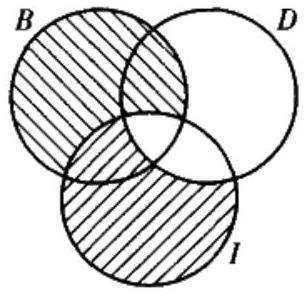
\includegraphics[max width=\textwidth, center]{2025_05_15_6a28331d5e7c993ad07ag-333}

有效,Barbara

没有 $M$ 是 $D$\\
所有 $B$ 是 $D$\\
所以,没有 $B$ 是 $M$\\
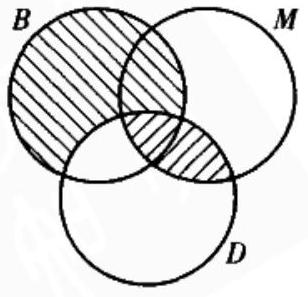
\includegraphics[max width=\textwidth, center]{2025_05_15_6a28331d5e7c993ad07ag-333(1)}

有效,Cesare

2.(1)没有有经验的人是无能的。\\
(2)杰金斯总是犯错。\\
(3)没有有能力的人总是犯错。\\
所以,杰金斯是没有经验的。\\
3.(1)图书馆中我没有推荐的书都是基调不健康的。\\
(2)精装书都是优秀作品。\\
(3)所有传奇小说是基调健康的。\\
(4)我并没有向大家推荐那些非精装书。\\
所以,图书馆中的所有传奇小说都是优秀作品。\\
4.(1)只有高深学者才能成为牛津大学的教师。\\
(2)没有心灵愚钝(insensitive)的人是音乐爱好者。\\
(3)没有心灵不敏感(not sensitive)的人能成为浪荡子。\\
(4)没有不爱好音乐的高深学者。\\
所以,所有牛津大学的教师是浪荡子。\\
*5.(1)没有有意义的诗歌不会受到高品位者的欢迎。\\
(2)没有现代诗歌能够不矫揉造作。\\
(3)你的所有诗歌都是谈及"肥皂泡"的。\\
(4)没有矫揉造作的诗歌会受到高品位者的欢迎。\\
(5)只有现代诗歌是谈及"肥皂泡"的。\\
所以,你的所有诗歌都是无意义的。\\
6.(1)除了作家没有人是诗人。\\
(2)只有军官是宇航员。\\
(3)给新杂志投稿的人都是诗人。\\
(4)没有既是军官又是作家的人。\\
所以,没有任何一个宇航员是新杂志投稿人。\\
II.下列每组命题都可以作为一个连锁三段论的前提,写出每组的结论,使之构成有效论证。\\
*1.(1)没有人读泰晤士报,除非是受过良好教育的人。\\
(2)没有刺猬会阅读。\\
(3)那些不会阅读的不是受过良好教育的。\\
2.(1)所有布丁都很好吃。\\
(2)这顿饭不是布丁。\\
(3)没有好吃的东西有益健康。\\
3.(1)医生给我的食谱上只有不油腻的食品。\\
(2)没什么适合我口味的东西可以作夜宵。\\
(3)婚礼蛋糕总是很油撼的食品。\\
(4)医生给我的食谱上的食品都是可以作夜宵的。\\
4.(1)我所有的女儿都很苗条。\\
(2)我的孩子中没有不参加体育锻炼而身体好的。\\
(3)我的孩子中所有贪食的都很胖。\\
(4)我的儿子中没有参加体育锻炼的。\\
*5.(1)如果我做逻辑习题时没有抱怨,你就能知道那是一道我会做的题目。\\
(2)这些连锁论证没有像我做过的题目那样按标准的顺序排列。\\
(3)容易的题目不会让我觉得头痛。\\
(4)我不会做那些不按标准顺序排列的题目,它们与我所做过的题目不同。\\
(5)我做题时从不抱怨,除非题目让我觉得头痛。

\section*{7.7 析取三段论和假言三段论}
至此,我们讨论的是关于直言三段论的分析,现在来看其他种类的三段论。我们称一个三段论是直言三段论,是因为其所包含的命题都是直言命题,即都是肯定或否定概念之间、类之间的包含或排斥关系。但一个三段论一一包含两个前提和一个结论的演绎论证——有可能包含不是直言命题的命题,这种三段论就不是直言三段论,而要根据所含命题的种类定名。因此,要形成对三段论推理的完整认识,我们还必须简要地考察其他种类的命题和由它们构成的三段论。

我们已经很熟悉的直言命题可以看做简单(simple)命题,它们都是对类与类之间关系的直接肯定或否定。与之不同,有些三段论论证使用的命题是包含不止一个支命题的复合(compound)命题,这些支命题又可以是任何种类的命题。

第一种复合命题叫做析取(disjunctive)命题或选言(alternative)命

题。例如,"或者斐多跑开了或者斐多被车撞倒了",两个支命题分别是 "斐多跑开了"和"斐多被车撞倒了"。这个析取命题,或叫析取句,包含两个支命题作为整个命题的析取支(disjunct)。析取命题并非直接肯定某个支命题为真,而是说至少它们当中有一个是真的,也不排除两个同时为真的可能。

如果以一个析取命题为前提,而另一个前提对其中一个支命题加以否定,或者说它与该析取支相矛盾,那么,就可以说有效地推出析取命题的另一个支命题为真。一个具有这种形式的论证,就是一个有效的析取三段论,例如:

\begin{displayquote}
或者斐多跑开了或者斐多被车撞倒了,斐多没有跑开,所以,斐多被车撞倒了。
\end{displayquote}

用刚刚定义的术语说,并不是每一个"析取三段论"都有效。比如下面 280这个论证:

\begin{displayquote}
或者斐多跑开了或者斐多被车撞倒了,斐多跑开了,所以,斐多没有被车撞倒。
\end{displayquote}

以上是个无效的析取三段论。表面上,它与第一个例子类似,但是容易看出它是一个逻辑谬误。假如出现斐多跑开并且被车撞倒的情况,并不与析取前提相冲突。对于一个析取式,肯定一个支命题为真,并不能推出另一个支命题为假,因为两个支命题可能同时为真。因此,只有用一个直言前提否定析取前提的一个析取支,从而肯定另一个析取支时,我们才说它是一个有效的析取三段论。

基于下面这个论证,有人可能对此提出异议:

或者史密斯在纽约或者史密斯在巴黎,\\
史密斯在纽约,\\
所以,史密斯不在巴黎。

其中的直言命题肯定了析取前提的一个析取支,结论否定了另一个析取支,而结论看起来是有效地得出的。然而,仔细分析可以表明,上面表述出来的析取命题在论证中实际上并没有起作用。结论是从省略了的前提中推出来的。未表达出来的前提是:"史密斯不能既在纽约又在巴黎",这是明显为真的。如果用析取命题表示之,即:

或者史密斯不在纽约或者史密斯不在巴黎。

显然,用这个揭示出来的前提代替原来的析取命题,所得到的新论证是一个明显有效的析取三段论。表面上的例外实际上不是例外,上述异议是不成立的。

第二种复合命题是条件(conditional)命题或假言(hypothetical)命题。例如"如果第一个土著人是政客,那么第一个土著人说谎"。一个条件命题由两部分组成,"如果"后面的命题叫做前件(antecedent),"那么"后面的命题叫做后件(consequent)。假如一个三段论所含命题都是条件命题,称为纯假言三段论。例如:

如果第一个土著人是政客,那么他说橫。\\
如果他说谎,那么他否认自己是政客。\\
所以,如果第一个土著人是政客,那么他否认自己是政客。

从这个论证中可以看到,第一个前提和结论有相同的前件,第二个前提和结论有相同的后件,而第一个前提的后件与第二个前提的前件相同。显然,任何具有如上关系前提与结论组成的纯假言三段论都是有效论证。

由一个条件前提和一个直言前提组成的三段论叫做混合假言三段论 (mixed hypothetical syllogism)。混合假言三段论有两种有效式,它们也都有各自的特别名称。第一种有效式例示如下:

如果第二个土著人说真话,那么只有一个土著人是政客。\\
第二个土著人说真话。\\
所以,只有一个土著人是政客。

其中,直言前提是对条件式前提的前件的肯定,结论是对后件的肯定。任何具有这样形式的论证都是有效的,这种有效式叫做肯定前件式(affirm- ative mood)或分离式(modus ponens)(这个词语来源于拉丁文 ponere,意思是"肯定")。绝不能把分离式与下面的无效式混为一谈:

\begin{displayquote}
如果培根写了《哈姆雷特》,那么他就是个大作家。\\
培根是个大作家。\\
所以,培根写了《哈姆雷特》。
\end{displayquote}

这个论证不同于分离式之处在于,其直言前提肯定的是条件前提的后件而不是前件。任何具有这种形式的论证都被称为犯了肯定后件谬误(fallacy of affirming consequent)。

混合假言三段论的另一种有效式例示如下:

\begin{displayquote}
如果独眼犯人看见的是两顶红帽子,那么他就能说出自己所戴帽子的颜色。
\end{displayquote}

\begin{displayquote}
独眼犯人不能说出自己所戴帽子的颜色。\\
所以,独眼犯人看见的并不是两顶红帽子。
\end{displayquote}

其中,直言前提是对条件前提后件的否定,结论是对前件的否定。任何具有这种形式的论证都是有效的,称为否定后件式(modus tollens)(来源于拉丁文 tollere,意思是"否定")。绝不能把这种形式与如下论证例示的无效式混为一谈:

\begin{displayquote}
如果卡尔贪污了学院的资金,那么卡尔犯了重罪。\\
卡尔没有贪污学院的资金。\\
所以,卡尔没有犯重罪。
\end{displayquote}

这个论证不同于否定后件式之处在于,其直言前提否定的是条件前提的前件而不是后件。我们称任何具有这种形式的论证犯了否定前件谬误(fal- lacy of denying antecedent)。

\section*{三段论的主要类型}
1.直言三段论,仅由肯定或否定类之间的包含或排斥关系的直言命题组成。例如:

所有 $M$ 是 $P$\\
所有 $S$ 是 $M$\\
所以,所有 $S$ 是 $P$ 。\\
2.析取三段论,前提包含一个析取(或选言)命题,它断言两个选言支至少一真,另一个前提断言其中一个选言支为假。例如:

或者 $P$ 是真的或者 $Q$ 是真的\\
$P$ 不是真的\\
所以,$Q$ 是真的。\\
3.假言三段论,包含一个或多个假言(或条件)命题,这种命题肯定如果其支命题之一(前件)为真,那么另一个支命题(后件)也是真的。可以再分为两个子类:

A)纯假言三段论,完全由条件命题组成。例如:\\
如果 $P$ 是真的,那么 $Q$ 是真的\\
如果 $Q$ 是真的,那么 $R$ 是真的\\
所以,如果 $P$ 是真的,那么 $R$ 是真的。\\
B)混合假言三段论,一个前提是条件命题,另一个是断定条件前提之前件为真的命题。例如:

如果 $P$ 是真的,那么 $Q$ 是真的\\
$P$ 是真的\\
所以,$Q$ 是真的。

\section*{练习题}
\section*{例题}
1.如果一个人不可能做他实际上所做以外的事情,那么他就可以不对自己的行为负责。但如果决定论是对的,那么,行为者的任何行为都是由于不可能做其他事情而做出的。因此,如果决定论是对的,则没有人对他所做的事负责。\\
-Winston Nesbit and Stewart Candlish, "Determinism and the Ability to Do Oth- erwise",Mind,July 1978

\section*{解答}
这是一个纯假言复合三段论,是有效式。\\
2.就这件事,我不能做更多。如果我做,我就不得不对大使说谎。但我不能说谎。\\
-Henry Bromell,"I Know Your Heart,Mar- co Polo",The New Yorker, 6 March 1978

3."J.J",我回答说,"如果这里有你的事,我就会请你来的。但这里没有你的事,所以我没有请你。"\\
--Paul Erdman,The Crash of'79\\
4.假如说,在经济事务中人的行为只能依据经济报酬或武力而行事,那么在现代社会中,动用武力尽管没有完全消失但已经不常用,因而只有经济报酬一直发挥重要作用。\\
-_John Kenneth Galbraith,The New Indus- trial State\\
*5.如果每个人都有一套确定的行为规则用以规范自己的生活,那么,他就不过是一台机器。但没有这样的规则,所以,人不会成为机器。\\
--A.M.Turing,"Computing Machinery and Intelligence",Mind,vol.59, 1950

6.史密斯是消防员或者是工程师,史密斯不是消防员,因此,史密斯是工程师。

7.如果第一个土著人是政客,那么第一个土著人否认自己是政客。第一个土著人否认自己是政客。因此,第一个土著人是政客。

8.如果第一个土著人否认自己是政客,那么第二个土著人说真话。如果第二个土著人说真话,那么第二个人不是政客。因此,如果第一个土

著人否认自己是政客,那么第二个土著人不是政客。\\
9.如果琼斯先生住在芝加哥,那么他就是个司闸员,琼斯先生住在芝加哥。因此他是个司闸员。\\
*10.如果第二个土著人说真话,那么第一个土著人否认自己是政客。如果第三个土著人说真话,那么第一个土著人否认自己是政客。因此,如果第二个土著人说真话,那么第三个土著人说真话。

11.如果罗宾森是司闸员,那么罗宾森住在芝加哥,罗宾森不住在芝加哥,所以他不是司闸员。

12.如果罗宾森是司闸员,那么史密斯是工程师,罗宾森不是司闸员,因此史密斯不是工程师。

13.如果琼斯先生是司闸员的邻居,那么 20000 美元就能平分成 3份,但 20000 美元不能平分成 3 份,所以,琼斯先生不是司闸员的邻居。

14.如果独眼犯人不知道自己所戴帽子的颜色,那么瞎眼犯人戴的就不是红帽。独眼犯人不知道自己戴的是什么颜色的帽子,因此,瞎眼犯人戴的不是红帽。\\
*15.史密斯是司闸员的邻居,或者罗宾森是司闸员的邻居。罗宾森不是司闸员的邻居,因此史密斯是司闸员的邻居。

16.如果三个犯人都戴白帽,那么独眼犯人就不知道自己所戴帽子的颜色。独眼犯人不知道自己帽子的颜色,因此三个人戴的都是白帽。

17.罗宾森住在底特律或者住在芝加哥,罗宾森住在底特律,所以他不住在芝加哥。

18.这个陌生人或者是流讯或者是俊瓜,这个陌生人是流讯,因此,他不是傻瓜。

19.如果三段论犯了肯定后件的谬误,则是无效式,这个三段论没有犯肯定后件的谬误,因此它是有效式。\\
*20.如果第一个土著人是政客,那么第三个土著人说真话。如果第三个土著人说真话,那么,第三个土著人不是政客。因此,如果第一个土著人是政客,第三个土著人就不是政客。

21.我确信人类从来没有认识到爱的力量,如果我们真的知道什么是爱,那么我们肯定会为爱神建起庄严的庙宇,筑起美丽的祭坛,举行最隆重的仪式。而实际上我们知道现在根本什么也没做。

22.我已经说过,他必定是到金斯皮兰或者到梅普里通去了。他现在不在金斯皮兰,那一定在梅普里通。\\
--A.Conan Doyle,The Adventure of Sliv- er Blaze

23.按照哈里德的计算,如果冥王星的直径在 4200 英里以上,那么就会有一个隐藏的星体出现在麦克唐纳星(发现于得克萨斯州的戴维斯堡)那里,以往的记载很明白地表明,并没有这种现象。因此,冥王星的直径必然等于或小于这个尺寸,不可能大于它。\\
-Thomas D.Nicholson,"The Enigma of Pluto",Natural History,March 1967\\
24.那么,这就是说事物或者是偶然的结果或者有其目的,而它们不可能是偶然或者自发产生的,所以,它们必有其目的。\\
-Aristotle,Physics\\
*25.没有这种情况(没有,甚至可以说,是不可能的):某个事物是它自己的作用因。因为在这样的情况下事物必须先于自身存在,这是不可能的。\\
-.Thomas Aquinas,Summa Theologiae,I, question 2,art. 3\\
26.钱财或者是种罪恶(evil)或者是善物(good),钱财不是一种罪恶,所以,钱财是善物。\\
-Sextus Empiricus,Against the logicians\\
27.可以肯定,如果其本质和动力是无限的,那么其善就是无限的,因为本质有限的东西只有有限的善。\\
-Roger Bacon,The Opus Majus\\
28.我现在确实是知道这支铅笔是存在的,但假如休谟的两个原理是对的,我就不知道了。因此,休谟的原理必定是错的(其中一个错或者两个都错)。\\
-G.E.Moore,Some Main Problems of Philosophy\\
29.一个无理论的状态是可能的,仅当没有证据理论。但是证据理论是存在的。所以,一个无理论的状态是不可能的。\\
-Henry W.Johnstone,Jr.,"The Law of Non-Contradiction",Logique et Analyse,\\
*30.显然,我们使用这些语词[例如物质(substance)、原因(cause)、变化(change)等等]表示某些东西,且每个都表示不同的东西。否则,我们就不能相容地使用它们。而事实上,从整体上说,我们确实在相容地使用并控制它们的。\\
--C.D.Broad,Scientific Thought\\
31.如果数是一种表象,算术就会是心理学。但正如天文学不是心理学一样,算数也不是。正如天文学不研究行星的表象而研究行星本身一样,算术的对象也不是表象。\\
-Gottlob Frege,The Foundations of Arith- metic

32.如果错误是某种肯定的东西,则其原因就是神,并且它应当经常为神所创造[命题12:凡存在之物仅由于神的力量才得以保存]。但这是荒谬的[命题 13:神是十分公正的,绝不会是骗子]。故错误不是某种肯定的东西。此证。\\
-Baruch Spinoza,The Principles of Philoso- phy Demonstrated by the Method of Geometry\\
33.……如果精神状态与物质状态是同一的,那么两者的所有性质都相同。但有一种性质,空间定位性,就不是两者共同的,也就是说,物质状态及结果都要占据空间位置,而精神结果及状态并不这样。因此,精神结果、状态与物质结果、状态不同。\\
— Jaegwon Kim,"On the Psycho-Physical I- dentity Theory",American Philosophi- cal Quarterly, 1966

34.当我们认为一个人应当为其行为承担道德责任时,他就会成为我们道德褒奖或责难的合法对象。但是显而易见,除非一个行动由一个"自由"(在其某种重要意义上)行动者所实施,否则该行动就不能成为道德褒奖或责难的合法对象。因此显然,某种意义上的自由意志可以说是道德责任的前提条件。\\
-C.Arthur Campbell,In Defence of Free Will\\
*35.三段论并非推理的重要工具……我们如果把三段论当做获得知识的唯一适当的工具和方法,那么就会得出:在亚里士多德以前,不曾有一个人通过或能够通过理性认识任何事物;而且自三段论法发明以后,一万

人中亦不曾有一个人凭其理性认知任何事物。不过上帝对人并不曾如此吝啬:把人仅只造成两足动物,留待亚里士多德使他有理性。

36."即将到来的是房产经济甚至整个经济的清冷时期,"美国民用建筑协会的首席经济学家米歇尔•萨米克阿斯特说道。\\
"没有好的房产经济,就不可能有整个经济的复苏;而房产经济将不会做好。"\\
——United Press report, 18 November 1980\\
37.尽管有限世界的说法十分流行,同时也遭到了广泛的批驳。有限世界必然有一个边界,也就是亚里士多德所说的最外圈(outmost sphere)。这是不可能的,因为一个边界只能把空间的一个部分同另一个部分隔开来。古希腊人就曾提出了这种反驳,而这种反驳也重新出现在早期文艺复兴时期的科学怀疑论中。现在研究这种问题的学生也提出了这种反驳。如果认可这样的反驳,就可以下结论说宇宙是无限的。\\
-J.J.Callahan,"The Curvature of Space in a Finite Universe",Scientific American, August 1976\\
38.如果他恳求斯大林——恳求斯大林改变工作方式——那么,斯大林可能会变得令人尊敬;如果斯大林令人尊敬,瓦迪姆就不得不敬畏他。但是对于这个人瓦迪姆只有憎恨。因此,他不会恳求斯大林,否则他会面临一个可怕的两难境地。\\
—William F.Buckley,Jr.,Who's on First?\\
39.如果每个人都奉行它的话,那么,完全的和平主义就是一个好原则。但并非每个人都奉行,所以和平主义不是好原则。



\section*{7.8 二难推论(The Dilemma)}
没有什么特别重要的地方。但从修辞角度看,二难推论是一种最有力量的说服工具之一一可谓论战中的一种致命性武器。\\
不严格地说,如果一个人必须在两种选项中做出决断,但两个选项都很糟糕或令人不愉快,那么,我们就说这个人"陷人"了两难(或者说进退维谷)之中。二难推论就是一种旨在使对手陷人这样境地的论证方式。在争论过程中,二难推论使得对手必须做出选择,但无论选择什么,都会得出一个他不能接受的结论。

理查德•费曼(Richard Feynman)是一位著名的物理学家,他在回忆1986年"挑战者"号爆炸的调查时,猛烈地抨击了(美国)国家航空航天局(NASA)的管理失误,他用的就是下面的二难推论:

\begin{displayquote}
我们每次问起高层管理者,他们都会说关于手下发生的事,他们什么都不知道……或者最高领导团确实不知道,这样他们就不知道应该知道的事,或者他们知道,这样他们就在对我们说说。 ${ }^{[7]}$
\end{displayquote}

如此的质问就将对手(此处指的是国家航空航天局的管理者们)推人两难境地,令他们无地自容。其中唯一明确表述的前提是一个析取命题,但析取支必定有一个为真,或者他们知道或者他们不知道手下发生的事。不管选择哪一方,结果对对手来说都是不利的。二难推论的结论本身也可以是一个析取命题(例如,"国家航空航天局的管理者或者不知道他们应该知道的事,或者他们说谎"),此时我们称之为复杂式(complex)二难推论。结论也可以是直言命题,这时就称之为简单式二难推论。

二难推论的结论并非总是令人不愉快的,如下简单式二难推论得出的就是个好结论:

如果天上的神明没有欲求,那么他们就会很满足,如果他们有欲求而能完全实现,那么他们也会很满足。他们或者没有欲求或者能完全实现欲求。总之,他们都会很满足。

二难推论的前提并没有特殊的顺序要求,提供选项的析取前提可前可后。表述选择后果的两个条件命题可以联合表述,也可分开陈述。二难推论常用省略式表述,结论一般都是显而易见的,无须表述出来。有一个例子取

自林肯总统的一封信,他为废止美国南部邦黑奴制度的宣言作了如下辩护:

此宣言如同法律一样,或者有效或者无效。如果无效,就没必要取消。如果有效,就不能取消。任何人都明白。 ${ }^{[8]}$

避开或驳斥二难推论的结论的方法有三种,它们也有各自的名称,都与二难的两个(或多个)"死角"有关。分别称为"绕过(或避开)死角法"、"直击(擒拿)一角法"、"构造反二难法"。它们并非证明二难推论形式无效,而是在不改变推论形式有效性的前提下,寻找避免结论的方法。

绕过死角法是拒斥其析取前提。这是常用的最容易的避开二难的手段。除非析取前提的两个支命题是矛盾关系,否则它们很有可能是假的。常用来说明这个方法的例示是给学生分级打分的例子,有人认为好的分数能激励学生更努力地学习。但学生们想出这样一个二难推论用来驳斥上述理论:

如果学生喜爱学习,那么就不需要激励。如果学生厌烦学习,那么激励也没有用。学生或者是喜爱学习的或者是厌烦学习,所以,激励是不需要的或者没用的。

该论证形式是有效的,但我们能用绕过死角法来反驳这个论证。其析取前提是假的,因为学生会有不同的学习态度:有的喜爱,有的厌烦,还有许多人不同于前两者。对于后面这些人来说,激励既是需要的也是可以发挥作用的。这种方法并不是证明结论为假,只是表明推论本身并没有给结论提供充足的理由。

如果析取前提穷尽了所有可能性,是不可驳倒的,就不能用上述方法了。必须有另外的方法来避开结论,其中之一就是直击一角法,即拒斥两个假言前提中的一个。要否定两假言前提的组合,我们只需否定其中的一个即可。直击一角,就是要试图表明条件前提至少一假。刚才驳斥学校分级打分的例子,所依据的条件前提之一是"如果学生喜爱学习,就不需要激励",反驳者可以争辩说,即使一个学生喜爱学习,也需要激励,好分数会带来额外的奖励,甚至能激励最勤奋的学生更认真地学习。这样一

来,就很可能得到好的回应一一原来的二难的一角就被击破了。\\
构造反二难法是最巧妙的方法,但并不总能令人信服,我们来看这是为什么。用这种方法驳斥给定的二难推论,需要构造另一个二难推论,它的结论与原来的结论相反。辩驳中可以使用任何一个二难推论,但最理想的反二难推论应当与原来的推论有相同的组成成分(直言命题)。

有个古老的例子能说明这种方法,相传雅典有一位母亲劝儿子不要从政时说道:

如果你主持公道,人们就会仇视你。如果你不主持公道,神灵们就会仇视你。你必定或者主持公道或者不主持公道,所以无论如何都会被仇视。

他的儿子反驳说:

如果我主持公道,神灵们就会施爱于我。如果我不主持公道,人们就会施爱于我。我必定或者主持公道或者不主持公道,所以我都会被爱。

在把二难推论作为强力工具的日常论辩中一般人的争论中,这种驳斥方法,从几乎相同的前提得到相反的结论,是种很不错的修辞手法。但如果更细致地研究,就会发现它们的结论并不像初看上去那样对立。

第一个二难推论的结论是儿子会被仇视(被人们或者被神灵们),而反二难的结论是儿子会被爱(被神灵们或被人们)。实际上两者完全是相容的。反驳用的反二难仅仅是建构了一个结论不同的论证而已。两个结论可能都是真的,因而这里并没有达成真正的反驳。但在唇枪舌剑的辩论中,并不需要细致分析,如果在公共争辩中出现这样的反驳,听众大多会把它当做对原论证的毁灭性攻击。

如此反驳并不能驳倒推理,而只是将注意力引向同一事情的不同方面,这从如下的二难推论可能看得更清楚。"乐观主义者"认为:

如果我工作,就能挣钱,如果赋闲在家,那么我乐得自在。我或者工作或者不工作,总之,我能挣钱或者乐得自在。

\section*{而悲观主义者却会给出这样一个反二难:}
如果我工作,就不能乐得自在,如果赋闲在家,就不能挣钱。或者工作或者不工作,总之,我或者不能乐得自在或者不能挣钱。

这些结论只能说明看问题的视角不同,并非对事实状况的意见不一致。通常讲二难推论,都要说到普罗塔哥拉(Protagoras)和欧提勒士 (Euathlus)之间著名的讼案。普罗塔哥拉是生活在公元前 5 世纪的希腊的一名教师,他开设了很多课程,其中最著名的是法庭辩护术,欧提勒士想跟他学习当一名律师,但他负担不起学费。于是两人定了一个契约,普罗塔哥拉先不收学费,等欧提勒士学成并在第一场官司中获胜时,再交学费。可是,欧提勒士学成之后,迟迟没有在法庭上进行辩护,普罗塔哥拉等得不耐烦了,于是把他的学生告上法庭,要求收回学费。欧提勒士忘记了"律师为自己的案子辩护乃属愚行"的格言,决定为自己进行辩护。审理开始后,普罗塔哥拉就用一个压倒性二难推论陈述己方要求:

如果欧提勒士打输了官司,那么他必须还我学费(根据法庭的判决),如果欧提勒士打赢了官司,那么他也必须还我学费 (根据我们之间的契约),或者他打输或者打赢官司,都必须还我学费。

情况看来对欧提勒士而言十分不利,但他已把修辞术学得很好,于是他向法庭提出了如下相反的二难推论:

如果我打赢了官司,我不必交学费(根据法庭的判决),如果我打输了官司,我也不必交学费(根据我们之间的契约),或者我打赢或者打输,都不必交学费。

如果你是法官,该如何判决呢?\\
注意欧提勒士的反二难的结论与普罗塔哥拉的结论的确不相容,一个确实是另一个的否定。这种相反二难推论与原来的二难推论的互相拒斥的

情况并不多见。在这样的情况下,前提就是不相容的,两个二难推论可用于澄清其中蕴涵的矛盾。

\section*{练习题}
讨论有可能驳斥下列推论的论证。

\section*{例题}
1.如果我们干涉虚假而有害言论的发表,那么,我们就会承担压制他人自由的罪名。但如果我们不干涉,那么我们自己就有失去自由的危险。我们必须在干涉与不干涉之间做出选择。因此,我们或者会承担压制他人自由的罪名,或者冒失去自由的危险。

\section*{解答}
采用绕过死角法是不行的,直击一角法比较合适。理由如下:(a)自由并不包括发表虚假有害的言论,或者(b)如果我们真实有益的言论反对虚假有害的言论,并不会有失去自由的危险。这样一来,通过反驳论证的要素,我们证明了"我们不会犯压制他人自由或没有失去自由的危险",从而合理地驳回原来的论证。

2.巡回审判法庭(Circuit Courts)或者有用或者没用。如果有用,没有一个州应当取消它们,如果没用,没有一个州应当保留它们。让我们在完全赞成与完全放弃之间做出选择吧。\\
-Abraham Lincoln,annual message to Congress, 3 December 1861\\
3.如果你告诉我的是我已经知道的,那么,你就不能扩充我的知识,而如果你告诉我的是我不知道的,那么,你说的我理解不了。你告诉我的或者是我已经知道的,或者是我不知道的。总之,你或者不能扩充我的知识或者你说的我理解不了。

4.如果你告诉我的不能扩充我的知识,那对我就没有什么价值。如果你说的我理解不了,对我也没什么价值。你说的或者不能扩充我的知识或者是我理解不了的,总之,对我都没有价值。\\
*5.如果演绎推理的结论超出了前提,则推理无效,而如果结论不超出前提,则不能带来新知。演绎推理的结论或者超出了前提或者不超出前提。因此,或者推理无效,或者不能带来新知。

6.如果演绎推理无效,就是无价值的,如果不能带来新知,也是无价值的。演绎推理或者无效或者不能带来新知。所以,演绎推理都是没有价值的。

7.如果这位军官是忠诚的,他就会恪守他的命令,如果他有头脑,他就能理解这些命令。这个军官或者没有恪守命令或者没有理解它们,所以他必定或者是不忠诚的或者是没头脑的。

8.如果他是不忠诚的,那么开除他就是合理的,如果他没有头脑,那么开除他也是合理的。他或者不忠诚或者没有头脑,开除他都是合理的。

9.如果这些国家维持和平,那么联合国是不必要的,如果这些国家挑起战争,那么联合国阻止战争的目标就不能成功。这些国家或者维持和平或者挑起战争。因此,联合国或者是不必要的或者不会成功(达到目标)。\\
*10.如果人是善的,就不需法律来防止错误行为,而如果人是恶的,法律就起不到阻止错误行为的作用,人或者是善的或者是恶的,总之都不需要法律。

11.亨利七世的御前大臣莫顿大主教以善于为国王逼税而闻名于世。他认为,应该强制生活奢侈的人缴纳高额税费,因为很显然,他们负担得起。也应该强制生活节俭的人缴纳高额税费,很明显,他们储蓄了大量生活费。无论选择哪种生活方式,都跑不出"莫顿之叉"。\\
-Dorothy Hayden,Winning Declarer Play\\
12.如果我们的某个党员在该问题有罪,你或者知道或者不知道。你要是知道,你就是不可原谅的,因为你没有指证此人、揭示事实。要是不知道,你也是不可原谅的,因为你做了这种断言,尤其是你无法证明但仍坚持这种断言。\\
------Abraham Lincoln,address at Cooper Institu- te,New York City, 27 February 1860\\
13.邪恶一旦得逞,其反对派必定面临一个二难。如果你保持沉默,你会被看做帮凶,以沉默的方式默许邪恶。如果你反抗,你就会被指责激起新的暴行。失败党派的行为不会有所适从。\\
-Edmund Burke,A Letter to a Member of the National Assembly

14.我们似乎不能从这个古老的二难中解脱出来:如果断定什么是 "差异",你就要去描述什么是"不是";而如果你去断定什么"不是"差异,你根本就什么也没说。\\
--F.H.Bradley,Appearance and Reality\\
*15.所有政治行为的目标或是维持现状或是改变现状。如果维持现状,就是希望阻止可能更糟的改变。如果改变现状,就是希望使情况变得更好。因此,所有政治行为都是受某种关于更好或者更糟的思想指导的。\\
--Leo Strauss,What Is Political Philoso- phy?\\
16.如果物体是运动的,它或者在它所在之处运动,或者在它所不在之处运动。但物体的运动既不在它所在之处(因它在那里),也不在它所不在之处(因它不在那里),因此没有物体运动。\\
-Sextus Empiricus,Against the Physicists\\
17.我这把年纪从一个城市流浪到另一个城市,不断改变流浪之所,不断被驱逐,这样的生活真是好极了!因为我非常明白,无论我去哪里,都会像在这里一样,有青年来听我谈话,如果我把他们赶走,他们会让他们的兄长来把我赶走;如果我不赶走他们,他们的父亲及其朋友会来驱赶我。\\
-Plato,Apology\\
18.如果苏格拉底死去,他或者在活着的时候死去,或者在死的时候死去。但他活着的时候不会死去,这是当然的,因为他还活着,还没有死。他死的时候也不会死去,因为他不可能死两次。因此苏格拉底没有死去。\\
--Sextus Empiricus,Against the Physicists\\
19.安慰剂的使用有难以解决的内在矛盾。使用安慰剂的过程必须建立在好的医患关系之上,但是,如果一方隐瞒某些重要信息,将会对这种关系造成什么影响呢?如果医生将事实告知患者,就会破坏安慰剂有效的基础;如果他不如实相告,就是在破坏诚信关系。\\
--Norman Cousins,Anatomy of an Illness\\
*20."分析悖论"(paradox of analysis)的基础是如下一个二难推论:一个分析句或者只是同语反复因而是平庸的,或者超出原来的含义因而是假

的。在语言哲学上有一个与之等价的问题:一个新术语或者能用既存的术语说明,因而是冗余的,或者不能用既存术语说明,那就没有"赋予意义"。\\
----Ernestn Gellner,Words and Things\\
21.艾伦•布卢姆(Allan Bloom)的《美国人的精神封闭》是一本大获成功的畅销书,其主要观点是:"我们的文化正在走下坡路,我们的思想已经崩溃了"。同其他几本畅销书一样,它们受到许多批判,评论家指出:"……如果这种书是好书,那么大众,远离庸俗、有教养的大众,就能赏识其价值——这种书的中心论点就是荒谬的。而如果书中的论证正确,那么大众只能欣赏水平低下的书籍,这种书的畅销除了销售量外并不能有什么名誉,这样一来,这几本书就不可能体现它们所宣扬的高品质文化素养,因而不可能是好书。"\\
---Tzvetan Todorov,"The Philosopher and the Everyday",The New Republic, 14 September 1987\\
22."新解释可接受二难"很有意思……可描述如下:一种有价值的解释,必定不能仅仅重复对思想家已有的解释。但如果解释要做到正确,又不能变更思想家原来的观点。\\
--George Kimball Plochman,Foreword to Frege's Logical Theory by Robert Sternfeld\\
23.司法委员会最后辩论结束后第一天宣布的美国最高法院对"美国诉尼克松案"(1974)的判决是关键的。如果总统公然反抗此判决,他将被弹劾。如果他遵守判决,很显然他将在证据前被弹劾。\\
-_Victoria Schuck,"Watergate",The Key Reporter,Winter 1975-1976\\
24.卡米萨……试图将支持安乐死的人置于一个古老的二难困境之上。情况或者是,受害者还没有遭受病痛,此时,他对安乐死的认可是不知实情的、猜测性的认可——他不会用协议来等待自己被杀死;或者是,他因病痛而失去理智、因药物作用而精神麻木,此时他根本没有健全的心智。

必须鼓励竞争精神。或者鼓励或者不鼓励竞争精神,因而或者没有和平或者不能进步。

26.总统的总结性论证可用一个十分简洁的形式表述。联邦政府的运作模式将或者充分依赖人民,或者不充分依赖人民。在第一种情况之下,选民接受不了的规划,因其依赖于人民,将被抑制。在其他情况之下,联邦政府没有人民的信赖,其侵犯性的计划将很容易被州政府所废除——詶政府将得到人民的支持。\\
— James Madison,The Federalist Papers, no. 46\\
27.不知那位从科勒(Cole)来的先生是否知道有一条关于个人借贷的利率不得高于 $12 \%$ 的法令,这条法令十分严厉,违反它将受到严重惩罚。如果他不知道,就太无知了,没有资格做委员会领导人;如果他知道,他就是避而不谈,这说明他不够坦率,不值得受到人们的尊敬和信任。\\
-Abraham Lincoln,speech in the Illinois legislature, 11 January 1837\\
28.……一个人既不能试着去发现他知道的东西,也不能试着去发现他不知道的东西。他不会去寻找他知道的东西,因为他既然知道,就没必要再去探索;他也不会去寻找他不知道的东西,因为在这种情况下,他甚至不知道自己该寻找什么。\\
-Plato,Meno\\
29.被关进精神病院的人逃不出如下不可解决的二难推论。"如果他承认有病,就证明他曾经是疯子。如果拒绝承认并表示抗议,就证明他仍然是疯子。"\\
——Lewis H.Gann,"Psychiatry:Helpful Servant or Cruel Master?"The Intercol- legiate Review,Spring 1982\\
-30.我们告诉委托人,在第一轮面试时,不要谈及金钱问题。如果一个人要的薪水过高,招聘者会觉得他支付不起。如果要的太低,你实际上等于说"我的能力不足以完成您交给我的任务"。\\
-_James Challenger,"What to Do and Not to Do When Job Hunting",U.S.News \textbackslash &

31."帕斯卡赌注"(Pascal's wager)在宗教史和赌博史上都相当著名。帕斯卡认为不可知论者——不能确定上帝是否存在的人——最好要赌上帝存在。如果上帝存在但他却不是个信仰者,那么就会受到惩罚,永受地狱之火的煎熬;而如果上帝不存在而他信仰上帝,他也不会因这个错误而受任何惩词。显然,赌注下在相信上帝一方的从一开始就占上风。\\
-Daniel Seligman,"Keeping Up",For-\\
tune, 7 January 1995

第7章概要

本章探究日常语言中的三段论论证,展示了三段论的不同形式,并给出了一些理解、运用和评价它们的方法。

7. 1 节介绍把三段论翻译为标准形式的必要技术,并说明了非标准三段论的几种不同情形。\\
7.2 节说明了如何将某些看似含有三个以上的项的论证恰当地转化为标准式……通过去除同义词、去除补类等方法。\\
7.3 节说明若非标准式三段论论证中的命题不是标准式直言命题,则需要把它们翻译为标准式,以便用文恩图或者三段论规则加以检验。还给出了九种不同类型的非标准式命题及其相应的翻译方法:

1.单称命题。\\
2.谓词为形容词或形容词短语,而非名词或类词项的直言命题。\\
3.主要动词不是标准的联项"是"或"不是"的直言命题。\\
4.标准形式的各成分都出现,却没有按标准顺序排列的陈述句。\\
5.量词不是"所有"、"没有"或"有"这些标准语词的直言命题。\\
6.用"只"、"只有"表述的排斥命题。\\
7.不含量词的直言命题。\\
8.完全不像标准式直言命题但可以有标准式翻版的命题。\\
9.用"除了"等表述的除外命题。\\
7.4 节说明了借助辅助参项,非标准直言命题向标准直言命题的协同翻译,这对于检验其有效性是必要的。\\
7.5 节、 7.6 节介绍了省略三段论,即省略三段论论证中某个构成命题的三段论;以及复合三段论,即由一组相互关联的命题组成的三段论论

证链。\\
7.7 节介绍另外的两种三段论:析取三段论和假言三段论,因其中包含选言命题或假言命题而得名。\\
7.8 节讨论二难推论的修辞学用法。其中的选言论证提供对手不愿接受的选项。本节说明并例示了三种驳斥二难推论的修辞方法:"绕过(或避开)死角法"、"直击(擒拿)一角法"、"构造反二难法"。

\section*{【注释】}
[1]见康德(Immanuel Kant)《纯粹理性批判》(Critique of Pure Reason,1787)第一章"概念分析论"之第二节。一个多世纪之后,罗素就此问题给出了另一种解释 [见《我的哲学发展》(My philosophical Development,p.66,1959)]:逻辑"不会有长足的发展",除非看出两种形式是"完全不同的",因为其中的一个(单称)把谓项加于特定的主项之上,而另一个(全称)表达的是两个谓项之间的关系。罗素的说法成为当时现代符号逻辑理论的核心观点,本书第 10 章有详细讨论。康德所说的是单称命题在传统三段论中的用法,他认为传统三段论是十分强大的逻辑工具。\\
[2]但在某些语境中,会有意地避开冠词"the",以便造成人们所需要的某种模糊效果。在采用联合国第 242 号决议时,即㭔吁以色列返还在1967年"六日战争" (Six-Day War)中夺取的"区域",大家都同意该决议的英语文本更具权威性,因为若用法语表述就必须用到定冠词(le territoire),相当于英文的 the territory("这……区域"),指的是所有被夺取的区域,而这恰恰是各方一致同意的英语文本所谨慎回避的说法。故英语中省略定冠词有其逻辑意义。\\
[3]David Hume,Dialogues Concerning Natural Religion,Pt. 2 (1779).\\
[4]U.S.v.Morrison,decided 15 May 2000.\\
[5]From H.W.B.Joseph,An Introduction to Logic(New York:Oxford University Press,1916).\\
[6]除第I 题的 4、6 小题之外,本节习题都取自 Lewis Carroll 的 Symbolic Logic(New York:C.N.Potter,1977)。部分有改动。\\
[7]James Gleick,Genius:The Life and Science of Richard Feymman(New York:Pan- theon Books,1992).\\
[8]见 Abraham Lincoln 1863年8月26日致 James C.Conkling 的信。

\section*{藛8密}
\section*{符号逻辑}
\section*{8.1 现代逻辑的待号语司}
8.2 合取、否定和析取待号\\
8.3 条件陈述与实质蕴涵\\
8.4 论证形式与论证\\
8.5 陈述形式与实质等值\\
8.6 逻辑等价\\
8.7 实质䔾涵怪论\\
8.8 三大"思想法则"

第8章概要

\section*{8.1 现代逻辑的符号语言}
我们一直在寻求对演绎论证进行分析和评估的技术。演绎理论旨在提供这样的技术,它已经发展出两个不同的分支来做这件工作:此前三章所考察的是经典逻辑或亚里士多德型逻辑,本章和下两章的主题则是现代符号逻辑。

然而,论证的分析和评估经常因其表述语言的特性(如英语或任何其他自然语言的特性)而非常困难。自然语言使用的语词可能是模糊的或歧义的,论证的结构可能是含混的,比喻和习语可能会引起混淆或误导,诉诸情感可能会引起混乱等,这些问题在第一部分已经探讨过了。要避免这些困难就要直接进人论证的逻辑核心,为此逻辑学家们构造了一种能避免自然语言缺陷的人工符号语言。使用这种符号语言能精确地表述论证。

符号也能便利我们对论证的思考。"由于符号系统之助,"一位杰出的现代逻辑学家写道,"我们几乎用眼睛就可以机械地进行推理转换,否则,这种转换本来要求大脑有很高的智能。"${ }^{[1]}$ 这似乎有点悖谬,但符号语言确实可以帮助我们不需大伤脑筋就能完成某些智力活动。

古代的和古典的逻辑学家们也承认某种特殊逻辑记号的价值。亚里士多德在自己的分析中就使用了变项,而如前面几章所表明,改进了的亚里士多德型逻辑也以很复杂的方式使用了符号。 ${ }^{[2]} 20$ 世纪又有很大的改进。

在现代逻辑中,处于核心地位的不是三段论(如亚里士多德传统上的),而是逻辑联结词,它们是每个演绎论证,不管是不是三段论,在其构成要素之间的关系中所必须运用的。命题和论证的内在结构是现代逻辑关注的焦点。要理解这种结构,我们必须首先掌握现代逻辑分析中所使用的一些特殊符号。

现代符号逻辑不受演绎论证要转换成三段论形式的制约(亚里士多德型逻辑受这种制约)。正如我们在第 7 章所见,那种工作是很费力的。不必进行这种转换使得我们可以更直接地追求演绎分析的目标。下面给出的现代逻辑的符号记法是分析论证的特别有力的工具。使用这种记法我们可以更全面地达到演绎逻辑的核心目标:区分有效论证和无效论证。

\section*{8.2 合取、否定和析取符号}
在本章,我们将关注一些如下述例子般简单的论证:

那个盲囚戴红帽子或者那个盲囚戴白帽子。\\
那个盲囚没戴红帽子。\\
因此,那个盲囚戴白帽子。

以及

如果鲁宾逊先生是那个司闸员的邻居,那么鲁宾逊先生住在底特律和芝加哥之间。

鲁宾逊先生不住在底特律和芝加哥之间。\\
因此,鲁宾逊先生不是那个司闸员的邻居。

这种类型的论证都至少包含一个复合陈述。研究这样的论证时,我们把所有陈述分为两个大类,即简单的和复合的。一个简单陈述就是一个不包含任何其他陈述作为其分支的陈述。臂如,"查理是整洁的"就是一个简单陈述。一个复合陈述就是包含另外一个陈述作为其分支的陈述。譬如,"查理是整洁的并且查理是可爱的"就是一个复合陈述,因为它包含两个简单陈述作为其分支。当然,一个复合陈述的分支陈述自身也可以是复合的。 ${ }^{[3]}$

\section*{A.合取}
复合陈述有几种不同类型,每种都需要有其逻辑记法。第一种复合陈述是合取。通过在两个陈述之间使用语词 and("和"、"并且"),可以形成它们的合取;被如此联结的两个陈述叫合取支。因此,复合陈述"查理是整洁的并且查理是可爱的"就是一个合取,它的第一个合取支是"查理是整洁的",第二个合取支是"查理是可爱的"。

语词"和"是个简短且便利的词,但除了联结陈述外,它还有其他一些用法。臂如,陈述"林肯和格兰特是同时代人"不是一个合取,而是一

个表达关系的简单陈述。为了有一个其唯一功能是合取地联结陈述的独特符号,我们引人圆点"•"作为合取符号。于是,前述合取可以写成"查理是整洁的-查理是可爱的"。更一般的,如果 $p$ 和 $q$ 代表任意两个陈述,它们的合取就写为 $p \cdot q$ 。

我们知道每个陈述是或真或假的。因此我们说,每个陈述都有一个真值,一个真陈述的真值是真,一个假陈述的真值是假。用这种"真值"概念,按照一个复合陈述的真值是完全由它的分支陈述的真值确定,还是由它的分支陈述的真值以外的任何其他东西确定,可以把复合陈述分成两个不同的种类。

我们把这种区分运用到合取上。两个陈述的合取的真值完全地由它的两个合取支的真值确定。如果它的两个合取支都是真的,该合取就是真的;否则它就是假的。基于这个原因,我们说合取是真值函项复合陈述,其合取支是它的真值函项分支。

然而,并非所有复合陈述都是真值函项的。例如,复合陈述"奥赛罗相信苔丝德蒙娜爱卡西奥"的真值,无论如何都不是由作为它的分支的简单陈述"苔丝德蒙娜爱卡西奥"的真值确定的,因为不管苔丝德蒙娜是否爱卡西奥,奥赛罗相信苔丝德蒙娜爱卡西奥仍然可以是真的。因此,"苔丝德蒙娜爱卡西奧"不是陈述"奥赛罗相信苔丝德蒙娜爱卡西奧"的真值函项分支,该陈述自身也不是一个真值函项复合陈述。

为当前目的起见,如果一个复合陈述中的某个分支被任何有相同真值但互相区别的陈述替换,其所得不同复合陈述相互之间有相同的真值,那么,我们就把这个复合陈述的分支定义为它的一个真值函项分支。这样,如果一个复合陈述的所有分支都是它的真值函项分支,我们就可以把该复合陈述定义为一个真值函项复合陈述。 ${ }^{[4]}$

我们将只关注真值函项复合陈述。因此,在本书的余下部分,我们将用术语简单陈述指称不是真值函项复合陈述的任何陈述。

一个合取就是一个真值函项复合陈述,因此,我们的圆点符号就是一个真值联结词。已知任何两个陈述 $p$ 和 $q$ ,它们只有四种可能的真值组合。这四种可能情形及每种情形下该合取的真值可以排列如下:

如果 $p$ 为真且 $q$ 为真,那么 $p \cdot q$ 为真。如果 $p$ 为真且 $q$ 为假,那么 $p \cdot q$ 为假。

如果 $p$ 为假且 $q$ 为真,那么 $p \cdot q$ 为假。\\
如果 $p$ 为假且 $q$ 为假,那么 $p \cdot q$ 为假。

如果我们分别用大写字母 $\mathbf{T}$ 和 $\mathbf{F}$ 代表真值"真"和"假",那么,一个合取的真值由其合取支的真值确定的情形,可以用"真值表"的方式更简明地刻画如下:

\begin{center}
\begin{tabular}{|ccc|}
\hline
$p$ & $q$ & $p \cdot q$ \\
\hline
T & T & T \\
T & F & F \\
F & T & F \\
F & F & F \\
\hline
\end{tabular}
\end{center}

该真值表可看做是圆点符号的定义,因为它表明了在每种可能情形下, 303 $p \cdot q$ 所拥有的真值。

我们将发现用大写字母缩写简单陈述很方便。为此,我们一般用一个有助于我们记住它所缩写的那个陈述的字母。于是,我们把"Charlie's neat and Charlie's sweet"(查理是整洁的并且查理是可爱的)缩写为 $N \cdot$ $S$ 。(1)在自然语言中,通过在两个谓项之间加"和"而不重复主项,可以使得合取支有相同主项的那些合取更简明甚或更自然。譬如,"拜伦是一个伟大的诗人并且拜伦是一个伟大的冒险家"就可以写成"拜伦是一个伟大的诗人和伟大的冒险家"。我们把后者看做和前者一样表示了同样的陈述,并且把它们无差别地符号化为 $P \cdot A$ 。同样,在自然语言中,如果一个合取的所有合取支都有相同的谓项,该合取通常被写成在两个主项之间加"和"而不重复谓项。例如,"刘易斯是一个著名的探险家并且克拉克是一个著名的探险家"可以写成"刘易斯和克拉克是著名的探险家"。这两种表述中的任何一个都可以符号化为 $L \cdot C$ 。

正如圆点号的真值表定义所表明的,一个合取是真的,当且仅当,它的合取支都是真的。但语词 and("和"、"并且")还有另外一种用法,其指谓的不只是(真值函项)陈述,还有"随之而来"的意味,即时序关联。例如,陈述"琼斯从纽约进入该国并且直接赶往芝加哥"是有意义的且可能是真的,而陈述"琼斯直接赶往芝加哥且从纽约进入该国"则几乎

\footnotetext{(1)在汉语中可采用汉语拼音首位字母的方式。
}不可理解。"他脱了鞋并且上了床"和"他上了床并且脱了鞋"之间也有很大的区别。 ${ }^{[5]}$ 对这样例子的更深人的把握,就需要一个不同于真值函项联结词用法的特殊符号。

请注意,自然语言语词"但是"、"还"、"也"、"仍然"、"尽管"、"然而"、"此外"、"虽然如此"等,甚至逗号和分号都可以用来把两个陈述联结成一个复合陈述,在合取的意义上来说,它们都可以用圆点符号表示。

\section*{B.否定}
在自然语言中,一个陈述的否定(或拒斥、否认)的形成通常是在原陈述前加一个"并非"。或者可以通过给一个陈述加一个前(后)缀"这是假的"或"事情并非如此",来表达该陈述的否定。通常用符号"~" (叫做"波浪号"或"波形号")来表示一个陈述的否定。例如,若用符号 M 表示陈述"所有人都是有死的",则陈述"并非所有人都是有死的"、 "有的人不是有死的"、"所有人都是有死的是假的",以及"情况并非是所 804 有人都是有死的"等都可以无差别地符号化为 $\sim M$ 。更一般的,如果 $p$ 是一任意陈述,则它的否定可写为 $\sim p$ 。显然,波浪号是一个真值函项算子。任何真陈述的否定都是假的,任何假陈述的否定都是真的。这一事实可以用真值表简明地刻画如下:

\begin{center}
\begin{tabular}{|cc|}
\hline
$P$ & $\sim P$ \\
\hline
T & F \\
F & T \\
\hline
\end{tabular}
\end{center}

这个真值表可以看做是否定符号"~"的定义。

\section*{C.析取}
在自然语言中,两个陈述的析取(或选言)是通过在它们中间插入语词"或"形成的。如此结合的两个分支陈述叫"析取支"(或"选声支")。

自然语言语词"或"很模糊,它有两个相关但可区分的含义。其中一个含义可以用陈述"保险金会因生病或失业而被取消"为例来说明。这里的含义显然是,不仅生病的人和失业的人没有保险金,而且那些既生病又失业的人也没有保险金。"或"的这种含义叫做弱的或相容的含义。当某一个析取支为其或者两个析取支都为真时,该相容析取式是真的;仅当两个析取支均为假时,这两个析取支构成的相容析取式是假的。相容意义上的"或"有"两者之一,可能两者都"之意。保险单里的这种精确含义与

合同和其他法律文本中的一样,可以用词组"和/或"给予明晰表达。\\
语词"或"也可以用做强的或不相容的含义,此时其含义不是"至少一个",而是"至少一个且至多一个"。如果餐馆的菜单上列有"沙拉或甜点",很清楚,它的意思是说,根据所标的就餐价格,就餐者可以点一种或另外一种,但不能两者都点。在保险单里要表达"或"的不相容的精确含义,通常要加上词组"二者不可得兼"。

我们把两个陈述的相容析取解释为断言至少其中有一个是真的,把它们的不相容析取解释为,断言至少其中有一个为真,但并非两者都为真。注意,这两种析取的含义有一部分是共同的。这部分共同含义——至少有一个析取支为真——是相容的"或"的全部含义,是不相容的"或"的部分含义。

尽管在现代自然语言中析取的表述很模糊,但在拉丁文中并不模糊。对应于上述"或"的两种不同含义,拉丁文有两个不同的语词。拉丁语词 vel 指谓弱的或相容的析取,aut 对应强的或不相容意义上的语词"或"。习惯上用 vel 的第一个字母来代表弱的、相容意义上的"或"。如果 $p$ 和 $q$是任意两个陈述,它们的弱的或相容的析取写为 $p \vee q$ 。相容析取符号 (叫"楔劈号",有时也叫做"$\vee$ 形号")也是一个真值函项联结词。一个弱析取为假,仅当它的两个析取支均为假。我们可以用真值表把楔劈号定义如下:

\begin{center}
\begin{tabular}{|ccc|}
\hline
$p$ & $q$ & $p \vee q$ \\
\hline
T & T & T \\
T & F & T \\
F & T & T \\
F & F & F \\
\hline
\end{tabular}
\end{center}

本节所举的第一个样本论证就是一个析取三段论 ${ }^{[6]}$ :

那个盲囚戴红帽子或者那个盲囚戴白帽子。\\
那个盲囚没戴红帽子。\\
因此,那个杗囚戴白帽子。

其形式特征可以描述为:第一个前提是一个析取;第二个前提是第一个前提的第一个析取支的否定;结论与第一个前提的第二个析取支一样。很显

然,无论对语词"或"作何种解释,即不管是相容析取还是不相容析取,如此定义的析取三段论都是有效的。 ${ }^{[7]}$ 既然像析取三段论这样的以析取为前提的典型有效论证,无论对语词"或"作何种解释都是有效的,那么,我们可以简单地把语词"或"翻译为逻辑符号"$V$",而不管语词"或"采取何种含义。一般的,只有通过对上下文进行严格考察,或明确追问说话者或写作者,才能发现其采取的是何种含义。如果我们约定把语词 "或"的任意一次出现都当做相容的,那么,这个通常难以解决的问题就可以避免。另一方面,如果通过附加词组"二者不可得兼"的方式,明确地表达了是不相容析取,那么,正如即将见到的,我们有符号方法来描述这种附加意义。

在自然语言中,当两个析取支有同样的主项或谓项时,用"或"来压缩它们的析取表述,而不必重复这两个析取支的公共部分,这是很自然的。例如,"或者史密斯是所有者或者史密斯是管理者"可以同等好地表述为"史密斯或是所有者或是管理者",并且两者中的任何一个都可以合适地符号化为 $O \vee M$ 。"或者瑞德有罪或者巴奇有罪"通常被陈述为"瑞德或者巴奇有罪",它们都可以符号化为 $R \vee B$ 。

语词"除非"(unless)通常用来形成两个陈述的析取。例如,"除非你努力学习,否则你考不好"可正确地符号化为 $P \vee S$ 。原因在于我们用 "除非"意指,如果一个命题不是真的,则另一个会是真的。上面的例子可以理解为"如果你不努力学习,你就会考不好"——这正是析取的要义,因为它断言其中一个析取支是真的,由此,如果其中一个是假的,则另外一个必定是真的。当然,你也可能努力学习了但考得不好。

然而语词"除非"有时也被用来传达比这更多的信息。它的意思可以是:一个或另一个命题是真的但并非两者都是真的。也就是说,"除非"意指不相容析取。例如,杰里米•边沁(Jeremy Bentham)写道:"政治上好的东西不可能在道德上是坏的,除非对大数目来说是好的算术规则,对小数目来说不好。"${ }^{[8]}$ 在此,作者的意思确实是说,两个析取支中至少有一个是真的,但他显然也暗示它们不能两者都真。"除非"的其他用法有点含混。当我们说,"野餐将举行,除非下雨"(或者,"除非下雨,野餐将举行"),我们的意思当然是,如果不下雨,将举行野餐。但我们是否有如果下雨就不举行野餐这样的意思呢?这是不清楚的。在这里和其他地方一样,把每个析取当成弱的或相容的是明智的做法;"除非"最好简单

地用楔劈号(V)来符号化。

\section*{D.标点符号}
在自然语言中,要使复杂陈述意义明确,标点符号是必需的。若没有大量不同的标点符号的使用,许多句子就会非常含混。譬如,给"The teacher says John is a fool"加不同的标点符号,它就会有很不相同的含义。 ${ }^{(1)}$ 有些语句加上标点才可以理解,如"Jill where Jack had had had had had had had had had had had the teacher's approval"。在数学中,标点符号也同样必要。在没有特别约定的情况下, $2 \times 3+5$ 不能确定指称某个特定的数,而在使用标点清楚地表明其成分如何组合的情形下,$(2 \times 3)+5$ 指称 $11,2 \times(3+5)$ 指称 16 。为了避免歧义和使意义明确,数学中的分组符号以圆括号()、方括号[]和大括号 \textbackslash {\} 等形式出现。 () 用来组合基本符号,[]用来组合包含圆括号的表达式,\textbackslash {\} 用来组合包含方括号的表达式。

在符号逻辑语言中,分组标点符号——圆括号、方括号、大括号——也是同样基本的。因为在逻辑中,复合陈述自身通常复合成一些更复杂的陈述。例如,$p \cdot q \vee r$ 是含混的:它可能意指 $p$ 与 $q$ 和 $r$ 的析取的合取,或者意指这样一个析取,其第一个析取支是 $p$ 和 $q$ 的合取,第二个析取支是 $r$ 。通过把公式加标点为 $p \cdot(q \vee r)$ 或 $(p \cdot q) \vee r$ ,我们可以区分这两种不同含义。不同标点方式所产生的差别,可以通过考察 $p$ 为假,$q$ 和 $r$都为真的情形看出。在这种情形中,第二个加标点的公式是真的(因为它的第二个析取支是真的),而第一个公式是假的(因为它的第一个合取支是假的)。在此,标点的不同导致了真和假的区别,因为不同的加标点方式会对含混的 $p \cdot q \vee r$ 赋不同的真值。

语词"either"(或者)在英语中有很多不同的意义和用法。在语句 "There is danger on either side"(两边都有危险)中,它有合取的力量。但它更常用来引入析取式的第一个析取支,如"Either the blind prisoner has a red hat or the blind prisoner has a white hat"(或者那个盲囚戴红帽子或者那个盲囚戴白帽子)。在此,它有助于语句修辞上的平衡,但并不影响语句的意义。"either"最重要的用法其实是给复合陈述加标点。例如,语句"The organization will meet on Thursday and Anand will be

\footnotetext{(1)此句可分别标点为:"The teacher says,John is a fool"(那个教师说约翰是優瓜)和 "The teacher,says John,is a fool"(约輸说那个教师是便瓜)。
}
elected or the election will be postponed"(那个组织星期四将开会并且安纳德会当选或者选举被推迟)是有歧义的,可以通过把"either"放在该语句的开头,或者把它插在名字"Anand"之前以消除歧义。在符号语言中,这种加标点的作用是通过加括号的方式实现的。前一段所讨论的那个含混公式 $p \cdot q \vee r$ 恰与刚才所考察的这个含混语句相对应。该公式的两种不同的加标点方式可与这个语句的两种不同的加标点方式相对应,而该语句的两种加标点方式是通过"either"的两种不同插人实现的。

析取的否定通常是用词组"不一也不"形成的。因此,陈述"或者费尔莫尔或者哈定是最伟大的美国总统"与陈述"费尔莫尔不是最伟大的美国总统,哈定也不是"矛盾。这个析取陈述可以符号化为 $F \vee H$ ,其否定或者是 $\sim(F \vee H)$ ,或者是 $(\sim F) \cdot(\sim H)$ 。(这两个符号公式的逻辑等价将在 8.5 节讨论。)应该清楚的是,否定断言两个陈述至少一真的析取式,要求把两个析取支都断言为假。

语词"两者都"在逻辑标点上扮演着重要角色,值得给予仔细的关注。正如上面所提到的,当我们说"杰玛和德勒克两者都不……"时,我们是说"杰玛不……德勒克也不……";我们是对他们每一个都进行否定。但当我们说"杰玛和德勒克并非两者都……"时,说的却是某件非常不同的事,我们是在对他们共同组成的对子进行否定,说的是"他们两者都……情况并非如此"。这种差别是非常根本的。在日常句子中,当"两者都"放在不同的地方时,会产生完全不同的意义。考虑下面语句意义的重要差别:

杰玛和德勒克不会两者都当选。\\
杰玛和德勒克两者都不会当选。

第一个语句否定的是合取 $J \cdot D$ ,可以符号化为 $\sim(J \cdot D)$ 。第二个语句是说他们中的每一个都不会当选,可以符号化为 $\sim(J) \cdot \sim(D)$ 。只需改变两个语词"两者都"和"不"的位置就改变了所断言的东西的逻辑力量。

当然,"两者都"并不总是扮演这种角色;有时只用它来增强语气。我们说"刘易斯和克拉克两者都是伟大的探险家",只是以之更强调地陈述"刘易斯和克拉克是伟大的探险家"所言说的东西。但在进行逻辑分析时,必须非常小心地确定"两者都"的标点符号作用。

为简化起见,即为了减少所需的括号数量,作如下约定是很便利的:在任意公式中,否定符号将被理解为施加于标点符号所管辖的最小陈述。没有这种约定,公式 $\sim p \vee q$ 是含混的,它意谓 $(\sim p) \vee q$ ,或者 $\sim(p \vee$ $q)$ 。但采用上述约定,其意指的就是备选者中的第一个,波浪号只能(根据约定)施加于第一个分支 $p$ ,而不是更大的公式 $p \vee q$ 。

为符号语言建立一套标点符号,不仅可以用来表述合取、否定和弱析取,而且也能够表述不相容析取。 $p$ 和 $q$ 的不相容析取式,断言它们当中至少有一个是真的,但并非两者都为真,可以简单地刻画为 $(p \vee q) \cdot \sim(p \cdot q)$ 。

任何仅用真值函项联结词——如圆点、波浪号和楔劈号——从简单陈述构造而成的复合陈述的真值,都完全由组成它的简单陈述的真或假确定。只要知道简单陈述的真值,它们的任何真值函项复合体的真值就很容易计算。在处理这样的复合陈述时,我们总是从它们最内部的组成分支开始,然后逐步外推。例如,设 $A$ 和 $B$ 都是真陈述且 $X$ 和 $Y$ 都是假陈述,即可计算复合陈述 $\sim[\sim(A \cdot X) \cdot(Y \vee \sim B)]$ 的真值如下:因为 $X$ 为假,故 $A \cdot X$ 为假,从而否定式 $\sim(A \cdot X)$ 为真;因为 $B$ 为真,故它的否定~ $B$ 为假,又因为 $Y$ 也为假,故 $Y$ 和 $\sim B$ 的析取 $Y \vee \sim B$ 亦为假;加方括号的公式 $[\sim(A \cdot X) \cdot(Y \vee \sim B)]$ 是一个真陈述和一个假陈述的合取,因此是假的;由此,它的否定即原整个陈述是真的。这样一种逐步程序,使得我们总能根据一个复合陈述的分支的真值来确定它的真值。

在某些情形下,即使我们不能确定一个或多个简单分支陈述的真或假,我们也能确定一个真值函项复合陈述的真值。首先通过假定某简单分支陈述为真,计算出该复合陈述的真值,然后假定该同一简单分支陈述为假,计算出该复合陈述的真值,对其真值未知的每个分支施行同样的步骤,我们就可以做到这一点。如果这些计算对被考察的复合陈述产生同样的真值,我们不必先确定它的分支的真值,就可以确定该复合陈述的真值,因为我们知道真值不是真就是假。

\section*{练习题}
I.用圆点、楔劈号和波浪号的真值表定义,确定下列陈述中哪些是真的。\\
'1.罗马是意大利的首都V罗马是西班牙的首都。

2.~(伦敦是英国的首都•斯德哥尔摩是挪威的首都)。\\
3.~伦敦是英国的首都•~斯德哥尔摩是挪威的首都。\\
4.~(罗马是西班牙的首都 $\vee$ 巴黎是法国的首都)。\\
*5.~罗马是西班牙的首都 $V \sim$ 巴黎是法国的首都。\\
6.伦敦是英国的首都 $V \sim$ 伦敦是英国的首都。\\
7.斯德哥尔摩是挪威的首都•~斯德哥尔摩是挪威的首都。\\
8.(巴黎是法国的首都•罗马是西班牙的首都)$V$(巴黎是法国的首都-~罗马是西班牙的首都)。

9.(伦敦是英国的首都 $\vee$ 斯德哥尔摩是挪威的首都)-(~罗马是意大利的首都-~斯德哥尔摩是挪威的首都)。\\
*10.罗马是西班牙的首都 $\mathrm{V} \sim$(巴黎是法国的首都•罗马是西班牙的首都)。

11.罗马是意大利的首都•~(巴黎是法国的首都 $\vee$ 罗马是西班牙的首都)。

12.~(~巴黎是法国的首都-~斯德哥尔摩是挪威的首都)。\\
13.~$\sim$(~罗马是西班牙的首都 $\vee \sim$ 巴黎是法国的首都)$\vee \sim$( $\sim$ 巴黎是法国的首都 $V$ 斯德哥尔摩是挪威的首都)〕。

14.~[~(~伦敦是英国的首都•罗马是西班牙的首都)-~(罗马是西班牙的首都-~罗马是西班牙的首都)〕。\\
*15.~[~(斯德哥尔摩是挪威的首都 $\vee$ 巴黎是法国的首都)$\vee \sim$( $\sim$ 伦敦是英国的首都 •~罗马是西班牙的首都)〕。

16.罗马是西班牙的首都 $V$( $\sim$ 伦敦是英国的首都 $V$ 伦敦是英国的首都)。

17.巴黎是法国的首都•~(巴黎是法国的首都•罗马是西班牙的首都)。

18.伦敦是英国的首都-~(罗马是意大利的首都-罗马是意大利的首都)。

19.(斯德哥尔摩是挪威的首都 $V \sim$ 巴黎是法国的首都)$V \sim$(~斯德哥尔摩是挪威的首都-~伦敦是英国的首都)。\\
*20.(巴黎是法国的首都 $V \sim$ 罗马是西班牙的首都)$V \sim$( $\sim$ 巴黎是法国的首都-~罗马是西班牙的首都)。

21.~[~(罗马是西班牙的首都•斯德哥尔摩是挪威的首都)$V \sim$\\
(~巴黎是法国的首都 V~罗马是西班牙的首都)]。\\
22.~[~(伦敦是英国的首都•巴黎是法国的首都)$V \sim$(~斯德哥尔摩是挪威的首都 $V \sim$ 巴黎是法国的首都)〕。

23.~[(~巴黎是法国的首都 $\vee$ 罗马是意大利的首都)•~(~罗马是意大利的首都 $V$ 斯德哥尔摩是挪威的首都)〕。

24.~[(~罗马是西班牙的首都 V 斯德哥尔摩是挪威的首都)•~(~斯德哥尔摩是挪威的首都 $V$ 巴黎是法国的首都)〕。\\
*25.~[(~伦敦是英国的首都•巴黎是法国的首都)$V \sim$( $\sim$ 巴黎是法国的首都•罗马是西班牙的首都)]。

II.如果 $A 、 B$ 和 $C$ 都是真陈述,并且 $X 、 Y 、 Z$ 是假陈述,下列复合陈述哪些是真的?\\
*1.$\sim A \vee B$\\
2.$\sim B \vee X$\\
3.$\sim Y \vee C$\\
4.$\sim Z \vee X$\\
5.$(A \cdot X) \vee(B \cdot Y)$\\
6.$(B \cdot C) \vee(Y \cdot Z)$\\
7.$\sim(C \cdot Y) \vee(A \cdot Z)$\\
8.$\sim(A \cdot B) \vee(X \cdot Y)$\\
9.$\sim(X \cdot Z) \vee(B \cdot C)$\\
*10.$\sim(X \cdot \sim Y)(B \cdot \sim C)$\\
11.$(A \vee X) \cdot(Y \vee B)$\\
12.$(B \vee C) \cdot(Y \vee Z)$\\
13.$(X \vee Y) \cdot(X \vee Z)$\\
14.$\sim(A \vee Y) \cdot(B \vee X)$\\
15.$\sim(X \vee Z) \cdot(\sim X \vee Z)$\\
16.$\sim(A \vee C) \vee \sim(X \cdot \sim Y)$\\
17.$\sim(B \vee Z) \cdot \sim(X \vee \sim Y)$\\
18.$\sim[(A \vee \sim C) \vee(C \vee \sim A)]$\\
19.$\sim[(B \cdot C) \cdot \sim(C \cdot B)]$\\
*20.$\sim[(A \cdot B) \vee \sim(B \cdot A)]$\\
21.$[A \vee(B \vee C)] \cdot \sim[(A \vee B) \vee C]$\\
22.$[X \vee(Y \cdot Z)] \vee \sim[(X \vee Y) \cdot(X \vee Z)]$\\
23.$[A \cdot(B \vee C)] \cdot \sim[(A \cdot B) \vee(A \cdot C)]$\\
24.$\sim\{[(\sim A \cdot B) \cdot(\sim X \cdot Z)] \cdot \sim[(A \cdot \sim B) \vee \sim(\sim Y \cdot \sim Z)]\}$\\
25.$\sim\{\sim[(B \cdot \sim C) \vee(Y \cdot \sim Z)] \cdot[(\sim B \vee X) \vee(B \vee \sim Y)]\}$

III.如果已知 $A$ 和 $B$ 为真,$X$ 和 $Y$ 为假,但不知 $P$ 和 $Q$ 的真值,能 311确定下列哪些复合陈述的真值?\\
*1.$A \vee P$\\
2.$Q \cdot X$\\
3.$Q \vee \sim X$\\
4.$\sim B \cdot P$\\
5.$P \vee \sim P$\\
6.$\sim P \vee(Q \vee P)$\\
7.$Q \cdot \sim Q$\\
8.$P \cdot(\sim P \vee X)$

9.$\sim(P \cdot Q) \vee P$\\
11.$(P \vee Q) \cdot \sim(Q \vee P)$\\
13.$\sim P \vee[\sim Q \vee(P \cdot Q)]$\\
15.$P \cdot[\sim(P \vee Q) \vee \sim P]$\\
17.$\sim[\sim(\sim P \vee Q) \vee P] \vee P$\\
19.$(\sim A \vee P) \cdot(\sim P \vee Y)$\\
*10.~Q•[(PVQ)•~P]\\
12.$(P \cdot Q) \cdot(\sim P \vee \sim Q)$\\
14.$P \vee \sim(\sim A \vee X)$\\
16.$\sim(P \cdot Q) \vee(Q \cdot P)$\\
18.$(\sim P \vee Q) \cdot \sim[\sim P \vee(P \cdot Q)]$\\
*20.~[PV(B•Y)]$\vee[(P \vee B) \cdot(P \vee Y)]$\\
21.$[P \vee(Q \cdot A)] \cdot \sim[(P \vee Q) \cdot(P \vee A)]$\\
22.$[P \vee(Q \cdot X)] \cdot \sim[(P \vee Q) \cdot(P \vee X)]$\\
23.$\sim[\sim P \vee(\sim Q \vee X)] \vee[\sim(\sim P \vee Q) \vee(\sim P \vee X)]$\\
24.$\sim[\sim P \vee(\sim Q \vee A)] \vee[\sim(\sim P \vee Q) \vee(\sim P \vee A)]$\\
-25.$\sim[(P \cdot Q) \vee(Q \cdot \sim P)] \cdot \sim[(P \cdot \sim Q) \vee(\sim Q \cdot \sim P)]$\\
N.用字母 $E 、 I 、 J 、 I$ 和 $S$ 分别缩写简单陈述"埃及食品短缺恶化"、"伊朗提高石油价格"、"约旦要求更多美国援助"、"利比亚提高石油价格"、"沙特阿拉伯多买 500 架战斗机",来符号化下列陈述。\\
*1.伊朗提高石油价格但利比亚不提高石油价格。\\
2.伊朗或利比亚提高石油价格。\\
3.伊朗和利比亚两国都提高石油价格。\\
4.并非伊朗和利比亚两国都提高石油价格。\\
*5.伊朗和利比亚两国都不提高石油价格。\\
6.伊朗或利比亚提高石油价格,但并非两国都如此。\\
7.沙特阿拉伯多买 500 架战斗机,并且或者伊朗提高石油价格或者约旦要求更多美国援助。

8.或者沙特阿拉伯多买 500 架战斗机并且伊朗提高石油价格,或者约旦要求更多美国援助。

9.并非埃及食品短缺恶化,并且约旦要求更多美国援助。\\
*10.埃及食品短缺恶化或者约旦要求更多美国援助,情形并非如此。\\
11.或者并非埃及食品短缺恶化,或者约旦要求更多美国援助。\\
12.埃及食品短缺恶化并且约旦要求更多美国援助,情形并非如此。\\
13.约旦会要求更多美国援助,除非沙特阿拉伯多买 500 架战斗机。\\
14.除非埃及食品短缺恶化,利比亚才会提高石油价格。\\
*15.伊朗不会提高石油价格,除非利比亚这样做。

16.除非伊朗和利比亚两国都提高石油价格,它们当中的任何一个都不会。

17.利比亚提高石油价格,并且埃及食品短缺恶化。\\
18.并非伊朗和利比亚都不会提高石油价格。\\
19.除非伊朗和利比亚两国都不提高石油价格,埃及食品会短缺恶化并且约旦会要求更多美国援助。\\
*20.伊朗提高石油价格且埃及食品短缺恶化,或者并非约旦要求更多美国援助且沙特阿拉伯多买 500 架战斗机。

21.埃及食品短缺恶化且沙特阿拉伯多买 500 架战斗机,或者,约旦要求更多美国援助或利比亚提高石油价格。

22.沙特阿拉伯多买 500 架战斗机,并且,或者约旦要求更多美国援助或者伊朗和利比亚两国都提高石油价格。

23.埃及食品短缺恶化或者约旦要求更多美国援助,但伊朗和利比亚两国都不提高石油价格。

24.埃及食品短缺恶化,但沙特阿拉伯多买 500 架战斗机且利比亚提高石油价格。\\
*25.利比亚提高石油价格且埃及食品短缺恶化;然而,沙特阿拉伯多买 500 架战斗机且约旦要求更多美国援助。

\section*{8.3 条件陈述与实质蕴涵}
当把语词"如果"放在第一个陈述之前,把语词"那么"放在第一个和第二个陈述之间来结合两个陈述时,如此构成的复合陈述就是一个条件陈述(也叫"假言陈述"、"蕴涵"或"蕴涵陈述")。在一个条件陈述中,跟在"如果"后面的分支陈述叫前件(或"蕴涵者",偶尔也叫"前式"),跟在"那么"后面的分支陈述叫后件(或"被蕴涵者",偶尔也叫"后式")。例如,"如果琼斯先生是那个司闸员的邻居,那么琼斯先生挣的钱是那个司闸员的三倍"是一个条件陈述,其中,"琼斯先生是那个司闸员的邻居"是前件,"琼斯先生挣的钱是那个司闸员的三倍"是后件。

一个条件陈述断言在其前件为真的任何情形下,它的后件也是真的。它并不断言其前件为真,而只是断言如果其前件为真,其后件也为真。它也并不断言其后件为真,而仅仅断言它的后件会为真,如果前件为真的

话。一个条件陈述的基本含义,是断言其前后件之间的某种关系以特定次序成立。要理解一个条件陈述的含义,我们必须理解何为蕴涵关系。\\
"蕴涵"一词不止一个含义。我们已经看到,在引进一个特殊的逻辑符号来表示日常语词"或者"的某个单一含义之前,区分它的不同含义是有用的。要是我们不这样做,日常语言的含混性就会影响我们的逻辑符号系统,妨碍我们达到所欲获得的明晰性和精确性。在我们把一个特殊的逻辑符号引入这种联系中之前,区分"蕴涵"或"如果一那么"的不同含义亦同样有用。

考查下面的四个条件陈述,它们每个都断言一种不同类型的蕴涵,都对应于一种不同含义的"如果…那么":

A.如果所有人都有死且苏格拉底是人,那么苏格拉底有死。

B.如果莱士里是单身汉,那么莱士里是未婚的。\\
C.如果把这张蓝色的石蕊纸放在酸液中,那么这张蓝色的石蕊纸会变红。

D.如果斯塔德輸掉了这场比赛,那么我就吞下我的帽子。

即使随意地观察一下这四个条件陈述也会发现,它们具有非常不同的类型。 A 的后件乃由它的前件逻辑地推出,而 B 的后件是根据其前件中的术语"单身汉"的定义而得来,而"单身汉"的定义就是未婚男人。C 的后件不是仅根据逻辑或其词项的定义从其前件推出,这种联系必须经验地发现,因为这里所陈述的蕴涵是因果关系。最后,D的后件既不是根据逻辑或定义从前件推得,也没有涉及因果性定律——就这个词的通常意义来说。大多数因果性定律,臂如物理学和化学中发现的那些定律,描述的是世界发生了什么,而不管人的希望或欲求如何。当然,没有这样一种定律和陈述 D 相联系。这个陈述表述的是说话者在某种特定的情形下以特定的方式行事的决策。

可见,这四个条件陈述的不同之处,就在于每个断言了其前件和后件之间的一种不同类型的蕴涵关系。但它们并非完全不同,它们所断言的都是蕴涵的类型。那么,它们是否存在任何可识别的共同含义,即是否存在尽管可能不是其中任何一个的完整含义,但是这些公认的不同种类蕴涵所

共有的部分含义呢?\\
关于探求共同的部分含义的重要性,我们可以回想一下对日常语词 "或"进行符号刻画的过程。那时我们是如下进行的。首先,在对比相容和不相容析取时,我们强调"或"的两种含义之间的区别。我们注意到,两个陈述的相容析取的意思是说,它们当中至少一个为真。不相容析取的意思是说,它们当中至少一个为真,但不是两者都为真。其次,我们注意到这两种类型的析取有一个共同的部分含义。这个部分的共同含义,即至少有一个析取支为真,被看做是弱的、相容的"或"的整个含义,是强的、相容的"或"的含义的一部分。然后,我们引入特殊符号"V"来表达这个共同的部分含义(它是"或"的弱意义上的整个含义)。最后,我们注意到,表达共同的部分含义的符号刻画也是对语词"或"在下述意义上的合适翻译,即可以把析取三段论作为一个有效的论证形式保留下来。我们承认把不相容的"或"翻译成符号"V",忽略和丢掉了它的部分含义。但由这种翻译所保留的那个部分含义,是析取三段论继续成为一个有效论证必需的全部东西。既然析取三段论是我们这里所关注的涉及析取的典型论证,那么,语词"或"的这种部分翻译——在某些情形,可以从它的"完全的"或"全部的"含义中抽取出来——对我们目前的目的是完全合适的。

现在,我们希望以同样的方式抽取日常语言辞组"如果一那么"的含义。第一步已经完成:我们已经强调了短语"如果一那么"对应于四种不同蕴涵的四种意义之间的区别。现在准备做第二步,即发现一个至少是所有这四种不同类型的蕴涵的含义的一部分的那种意义。

要解决这个问题,可先看什么情形足以确立一个给定条件陈述的假。在什么情形下,我们会同意下面的条件陈述为假呢?

\begin{displayquote}
如果把这张蓝色的石蘂纸放进那种溶液中,那么这张蓝色的石蕊纸会变红。
\end{displayquote}

这个条件陈述并未断言任何一张蓝色的石蕊纸实际上被放进了这种溶液中,或任何一张蓝色的石蕊纸实际上变红了,认识到这一点是很重要的。它仅仅断言如果把这张蓝色的石総纸放进那种溶液中,那么这张蓝色的石蕊纸会变红。如果这张蓝色的石䓗纸实际上被放进这种溶液中,并且它没

变红,就证明该陈述是假的。可以说,当一个条件陈述的前件为真时,就获得一个关于该条件陈述的虚假性的严峻检验,因为如果它的后件为假且前件为真,该条件陈述本身就被证明为假。

对任一条件陈述"如果 $p$ 那么 $q$"来说,如果已知合取 $p \cdot \sim q$ 为真,也就是说,如果它的前件为真且后件为假,则可知该条件陈述为假。而若一个条件陈述为真,则上面所示合取式必定为假,也就是说,它的否定 $315 \sim(p \cdot \sim q)$ 必定为真。换句话说,对任何为真的条件陈述"如果 $p$ 那么 $q$"而言,它的前件和后件的否定的合取的否定,即 $\sim(p \cdot \sim q)$ ,必定也为真。据此,我们可把~$(p \cdot \sim q)$ 当做"如果 $p$ 那么 $q$"的含义的一部分。

每个条件陈述都意谓否定其前件为真且后件为假,但这不必是其整个含义。前面的 A 那样的条件陈述还断言了其前件和后件之间的一种逻辑联系,B 那样的条件陈述还断言了一种定义性联系,C 那样的条件陈述还断言了一种因果性联系,而 D 那样的条件陈述则还断言了一种决策性联系。但不管一个条件陈述断言的是何种蕴涵,它的一部分含义是对其前件和后件的否定的合取的否定。

现在,我们引进一个特殊的符号来表达短语"如果一那么"的这种共同的部分含义。通过以 $p \supset q$ 缩写 $\sim(p \cdot \sim q)$ ,我们来定义新符号"つ" (叫"马蹄号")。符号"つ"的确切含义可以用真值表方法揭示如下:

\begin{center}
\begin{tabular}{|l|l|l|l|l|l|}
\hline
$p$ & $q$ & $\sim q$ & $p^{\cdot \sim q}$ & $\sim(p \cdot \sim q)$ & $p$ つ $q$ \\
\hline
T & T & F & F & T & T \\
\hline
T & F & T & T & F & F \\
\hline
F & T & F & F & T & T \\
\hline
F & F & T & F & T & T \\
\hline
\end{tabular}
\end{center}

其中,前两列是导引列,它们只是列出 $p$ 和 $q$ 真值组合的所有可能情形。第三列据第二列得来,第四列据第一和第三列得来,第五列据第四列得来,根据定义,第六列与第五列真值相同。

符号"コ"不应被看成是指谓"如果一那么"的某种含义,或代表 (上列蕴涵类型中的)某种蕴涵关系。那是不可能的,因为没有单一的 "如果一那么"的含义,而是有几个含义。不存在该符号所刻画的单一蕴涵关系,而是有几种不同的蕴涵关系。故符号"つ"不应被看成是代表 "如果一那么"的所有含义。这些含义各不相同,用单个逻辑符号来缩写

所有这些含义的任何企图都会使符号变得含混,正如日常语言辞组"如果一那么"或"蕴涵"一样含混。符号"つ"是完全不含混的。 $p \supset q$ 缩写的就是 $\sim(p \cdot \sim q)$ ,它的含义包含在被探讨的各种蕴涵的含义之中,但它并不构成它们中任何一个的完整含义。

既然读 $p \supset q$ 的一种方便方式是"如果 $p$ 那么 $q$",我们也可以把符号 "D"看成表示了另一种蕴涵,而且这样做是很有好处的。但它不是与前面提到过的任何一种蕴涵相同的蕴涵,它被逻辑学家叫做实质蕴涵。给出这个特殊的名称,就是承认它是一个特殊概念,不应该把它和其他更常见类型的蕴涵相混淆。

日常语言中的所有条件陈述并非都必须断言前面所讨论的四种蕴涵之一。实质蕴涵实际上也是日常话语中所断言的第五种蕴涵。考虑这样一个评论:"如果希特勒是军事天才,那么我是猴子的叔叔"。很显然,它不是断言逻辑的、定义性的或因果性的蕴涵。它也不表达决策性蕴涵,因为说话者并没有能力使后件为真。这里的前后件之间没有"真正的联系",不管是逻辑的、定义性的还是因果性的。这种条件陈述经常被当做一种强调或幽默的方法来使用,它否定的是其前件,其后件通常是一个滑稽的、显然为假的陈述。既然没有任何为真的条件陈述有这样的真前件和假后件,那么,肯定这样一个条件陈述就意味着否定它的前件为真。上述条件陈述的完整含义就是,只要"我是猴子的叔叔"为假,即可否定"希特勒是军事天才"为真。既然前者明显为假,该条件陈述必被理解为否定后者。

这里的关键在于,实质蕴涵没有表明前后件之间的"实在关联",实际上,它所断言的仅仅是并非后件为假时前件为真。请注意:实质蕴涵符号像合取和析取符号一样,是真值函项联结词。它可用真值表定义如下:

\begin{center}
\begin{tabular}{|ccc|}
\hline
$p$ & $q$ & $p \supset q$ \\
\hline
T & T & T \\
T & F & F \\
F & T & T \\
F & F & T \\
\hline
\end{tabular}
\end{center}

正如这个真值表定义所表明,马蹄符"つ"有几个乍看起来很奇怪的特征:假前件实质蕴涵真后件的断言是真的;假前件实质蕴涵假后件的断言也是真的。这种表面的怪异可以由下面的探讨得到部分驱散。因为数 2 比数 4 小 (用符号表示为 $2<4$ ),可以推出任何小于 2 的数都小于 4 。条件公式:

如果 $x<2$ 那么 $x<4$\\
对任一 $x$ 都是真的。我们来看数 $1 、 3$ 和 4 ,依次以它们中的每一个代人前述条件公式的数字变项 $x$ ,可以观察到如下结果:

如果 $1<2$ 那么 $1<4$\\
在这种情形下,前后件都是真的,该条件陈述当然也是真的。\\
如果 $3<2$ 那么 $3<4$\\
在这种情形下,前件为假且后件为真,该条件陈述当然也是真的。\\
如果 $4<2$ 那么 $4<4$\\
在这种情形下,前件和后件都是假的,但该条件陈述仍然是真的。这三种情形分别对应于马蹄符"コ"的真值表定义中的第一、第三和第四行。可见,在一个条件陈述的前后件皆为真、前件为假且后件为真或前后件皆为假时,该条件陈述应该为真,这一点并不特别令人奇怪或惊讶。当然,没有小于 2 且不小于 4 的数,也就是说,没有其前件为真且后件为假的真条件陈述。这恰好是"つ"的真值表定义所表明的。

现在,我们打算把词组"如果——那么"的任何一次出现翻译成逻辑符号 "つ"。这种处理方式的意思是说,在把条件陈述翻译成符号时,我们把它们都只看做是实质蕴涵。当然,大多数条件陈述断言,在前后件之间不只实质蕴涵成立。因此,这种处理方式即意味着在把一个条件陈述翻译成符号语言时,应该忽略、撇开或"抽掉"它的部分含义。怎样辩护这种处理方式呢?

前面对用符号"$V$"来翻译相容和不相容析取这个处理方式的辩护是基于这样的理由:即使忽略附着在不相容析取"或"之上的附加含义,析取三段论的有效性也得到了保留。我们现在提议用符号"$\supset$"把所有的条件陈述仅翻译成实质蕴涵,可用完全同样的方式得到辩护。许多论证包含各种不同类型的条件陈述,但是,即便忽略这些论证的条件陈述的附加含义,我们所关注的一般类型的有效论证的有效性也都得到了保留。当然,这一点还需要证明,这是本章下一节的主题。

条件陈述可用多种不同方式表述。如下陈述:

如果他有一个好律师,那么他会被宣判无罪。

可以不用"那么"而被同样适当地表述为:

如果他有一个好律师,他会被宣判无罪。

前件和后件的表述次序可以颠倒,此时"如果"仍应在前件之前:

他会被宣判无罪,如果他有一个好律师的话。

显然,在上面所给的任何一个例子中,语词"如果"可被诸如"一旦"、318 "假如"、"倘若"或"在……条件下"等短语代替,而含义没有任何改变。经措辞调整还可把上述条件陈述表述为:

他有一个好律师蕴涵他会被宣判无罪。

或

他有一个好律师涵衍(entail)他会被宣判无罪。

从主动语态到被动语态的转换伴随着前后件次序的颠倒,可得其逻辑等价表述:

他会被宣判无罪被他有一个好律师所蕴涵(或涵衍)。

上列表述均可符号化为 $L \supset A$ 。\\
必要条件和充分条件的观念提供了条件陈述的其他一些表述形式。对任何一个特定事件来说,它的出现需要有许多必要情境。例如,一辆正常的轿车要能行使,油箱里有油,火花塞被校准,油泵能运转等都是必要条件。因此,如果该事件出现,它的出现所必需的每个条件必定都已经得到满足。据此,下述陈述:

油箱里有油是轿车行驶的一个必要条件。

可以同样适当地表述为:

轿车行使仅当它的油箱里有油。

它是如下说法的另一方式:

如果轿车行使,那么它的油箱里有油。

这些表述形式中的任何一个都可以符号化为 $R \supset F$ 。一般地说,"$q$ 是 $p$ 的必要条件"和"$p$ 仅当 $q$"可以符号化为 $p \supset q$ 。

对某特定情形而言,会有许多备选条件,它们中的任何一个都足以产生该情形。例如,就一个钱包里不止一美元来说,它里面有 101 便士、21个五分镍币、 11 个一角的硬币、 5 个两角五分钱等都是充分条件。如果获得其中的任何一个条件,那个特定的情形就会实现。因此,说"那个钱包里有 5 个两角五分钱是它里面超过一美元的充分条件",与说"如果那个钱包里有 5 个两角五分钱,那么它里面超过一美元"是一样的。一般的, "$p$ 是 $q$ 的充分条件"被符号化为 $p \supset q$ 。

如果 $p$ 是 $q$ 的一个充分条件,我们就有 $p \supset q$ ,并且 $q$ 必定是 $p$ 的一个必要条件。如果 $p$ 是 $q$ 的一个必要条件,我们就有 $q \supset p$ ,并且 $q$ 必定是 $p$ 的一个充分条件。因此,如果 $p$ 是 $q$ 的必要且充分条件,那么,$q$ 是 $p$的充分且必要条件。

并非每个含有"如果"(或类似语词)的陈述都是条件陈述。下列陈述中没有一个是条件陈述:"冰箱里有食品,如果你想吃","您的桌子准备好了,如果您乐意的话","假如感兴趣,有个消息给你","即便没得到允许,会议也会举行"。特定语词的出现与否决不是决定性的。在每种情形下,必须先理解给定语句的含义,然后用符号公式重新表述这种含义。

语词"如果"和"不确定的"之间没有必然的或逻辑的联系,尽管经常有这样一种说法:跟在语词"如果"后面的东西有点不确定。这一点可由下面的逸事所例示:

有一次,乔治•伯纳德•肖给温斯顿•丘吉尔送了两张他的新剧的首演式的票,附言"带一个朋友——如果你有的话";对

此,丘吉尔回复说他忙于出席别的首演式,但他会很感激第二场演出的票,"如果有这样一张票的话"${ }^{[9]}$ 。

\section*{练习题}
I.如果 $A 、 B 、 C$ 是真陈述,而 $X 、 Y 、 Z$ 是假陈述,用马蹄号、圆点号、楔劈号和波浪号的真值表确定下列哪些陈述是真的。\\
*1.$A \supset B$\\
2.$A \supset X$\\
3.$B \supset Y$\\
4.$Y \supset Z$\\
*5.$(A \supset B) \supset Z$\\
6.$(X \supset Y) \supset Z$\\
7.$(A \supset B) \supset C$\\
8.$(X \supset Y) \supset C$\\
9.$A \supset(B \supset Z)$\\
*10.$X \supset(Y \supset Z)$\\
11.$[(A \supset B) \supset C] \supset Z$\\
12.$[(A \supset X) \supset Y] \supset Z$\\
13.$[A \supset(X \supset Y)] \supset C$\\
14.$[A \supset(B \supset Y)] \supset X$\\
*15.$[(X \supset Z) \supset C] \supset Y$\\
16.$[(Y \supset B) \supset Y] \supset Y$\\
17.$[(A \supset Y) \supset B] \supset Z$\\
18.$[(A \cdot X) \supset C] \supset[(A \supset C) \supset X]$\\
19.$[(A \cdot X) \supset C] \supset[(A \supset X) \supset C]$\\
*20.$[(A \cdot X) \supset Y] \supset[(X \supset A) \supset(A \supset Y)]$\\
21.$[(A \cdot X) \vee(\sim A \supset X)] \supset[(A \supset X) \cdot(X \supset A)]$\\
22.$\{[A \supset(B \supset C)] \supset[(A \cdot B) \supset C]\} \supset[(Y \supset B) \supset(C \supset Z)]$\\
23.$\{[(X \supset Y) \supset Z] \supset[Z \supset(X \supset Y)]\} \supset[(X \supset Z) \supset Y]$\\
24.$[(A \cdot X) \supset Y] \supset[(A \supset X) \cdot(A \supset Y)]$\\
*25.$[A \supset(X \cdot Y)] \supset[(A \supset X) \vee(A \supset Y)]$

II.如果已知 $A 、 B$ 为真,$X 、 Y$ 为假,但不知道 $P$ 和 $Q$ 的真值,能 320确定下列哪些陈述的真值?\\
-1.$P \supset A$\\
2.$X \supset Q$\\
3.$(Q \supset A) \supset X$\\
4.$(P \cdot A) \supset B$\\
'5.$(P \supset P) \supset X$\\
6.$(X \supset Q) \supset X$\\
7.$X \supset(Q \supset X)$\\
8.$(P \cdot X) \supset Y$\\
9.$[P \supset(Q \supset P)] \supset Y$\\
*10.$(Q \supset Q) \supset(A \supset X)$\\
11.$(P \supset X) \supset(X \supset P)$\\
12.$(P \supset A) \supset(B \supset X)$\\
13.$(X \supset P) \supset(B \supset Y)$\\
14.$[(P \supset B) \supset B] \supset B$\\
-15.[ $(X \supset Q) \supset Q] \supset Q$\\
16.$(P \supset X) \supset(\sim X \supset \sim P)$\\
17.$(X \supset P) \supset(\sim X \supset Y)$\\
18.$(P \supset A) \supset(A \supset \sim B)$\\
19.$(P \supset Q) \supset(P \supset Q)$\\
*20.$(P \supset \sim \sim P) \supset(A \supset \sim B)$\\
21.$\sim(A \cdot P) \supset(\sim A \vee \sim P)$\\
22.$\sim(P \cdot X) \supset \sim(P \vee \sim X)$\\
23.$\sim(X \vee Q) \supset(\sim X \cdot \sim Q)$\\
24.$[P \supset(A \vee X)] \supset[(P \supset A) \supset X]$\\
*25.$[Q \vee(B \cdot Y)] \supset[(Q \vee B) \cdot(Q \vee Y)]$\\
III.用大写字母缩写所涉及的简单陈述,符号化下列陈述。\\
*1.如果阿根廷调集军队,那么,如果巴西向联合国抗议,那么智利会要求召开拉丁美洲国家全体会议。

2.如果阿根廷调集军队,那么,或者巴西会向联合国抗议,或者智利会要求召开拉丁美洲国家全体会议。

3.如果阿根廷调集军队,那么,巴西会向联合国抗议且智利会要求召开拉丁美洲国家全体会议。

4.如果阿根廷调集军队,那么,巴西会向联合国抗议,并且智利会要求召开拉丁美洲国家全体会议。\\
-5.如果阿根廷调集军队并且巴西会向联合国抗议,那么,智利会要求召开拉丁美洲国家全体会议。

6.如果阿根廷调集军队或者巴西向联合国抗议,那么,智利会要求召开拉丁美洲国家全体会议。

7.或者阿根廷会调集军队,或者如果巴西向联合国抗议,那么智利会要求召开拉丁美洲国家全体会议。

8.如果阿根廷不调集军队,那么,或者巴西不会向联合国抗议,或者智利不会要求召开拉丁美洲国家全体会议。

9.如果阿根廷不调集军队,那么,巴西不会向联合国抗议,智利也不会要求召开拉丁美洲国家全体会议。\\
*10.并非如果阿根廷调集军队,那么,巴西会向联合国抗议且智利会要求召开拉丁美洲国家全体会议。

821\\
11.如果并非阿根廷调集军队,那么巴西不会向联合国抗议,且智利会要求召开拉丁美洲国家全体会议。

12.巴西会向联合国抗议,如果阿根廷调集军队。\\
13.巴西向联合国抗议,仅当阿根廷调集军队。\\
14.智利会要求召开拉丁美洲国家全体会议,仅当阿根廷调集军队且

巴西向联合国抗议。\\
*15.巴西向联合国抗议,仅当或者阿根廷调集军队,或者智利要求召开拉丁美洲国家全体会议。

16.阿根廷会调集军队,如果或者巴西向联合国抗议,或者智利要求召开拉丁美洲国家全体会议。

17.巴西向联合国抗议,除非智利要求召开拉丁美洲国家全体会议。\\
18.如果阿根廷调集军队,那么,除非智利要求召开拉丁美洲国家全体会议,巴西才会向联合国抗议。

19.巴西不会向联合国抗议,除非阿根廷调集军队。\\
*20.除非智利要求召开拉丁美洲国家全体会议,巴西才会向联合国抗议。

21.阿根廷调集军队是巴西向联合国抗议的充分条件。\\
22.阿根廷调集军队是智利要求召开拉丁美洲国家全体会议的必要条件。

23.如果阿根廷调集军队且巴西向联合国抗议,那么,智利和多米尼加共和国都会要求召开拉丁美洲国家全体会议。

24.如果阿根廷调集军队且巴西向联合国抗议,那么,智利或多米尼加共和国会要求召开拉丁美洲国家全体会议。\\
*25.如果智利和多米尼加共和国都不要求召开拉丁美洲国家全体会议,那么,巴西不会向联合国抗议,除非阿根廷调集军队。

\section*{8.4 论证形式与论证}
\section*{A.运用逻辑类推进行反驳}
本节我们将更精确地阐明术语"有效"的含义。通过探讨运用逻辑类推进行反驳的方法,我们把形式定义与某些更熟悉的、直觉的观念联系起来。 ${ }^{[10]}$ 兹以如下论证为例:

培根是一位伟大的作家。\\
因此,培根写了那些通常归功于莎士比亚的剧本。

我们可能同意其前提但不同意其结论,从而断定该论证无效。证明无效性的方式之一就是运用逻辑类推的方法。我们可以反驳说,"你是否也可以这样来论证",

如果华盛顿是被暗杀的,那么华盛顿死了。\\
华盛顿死了。\\
因此,华盛顿是被暗杀的。\\
"但你不可能对该论证进行严格的辩护",我们可以继续说,"因为在这里,已知前提为真且结论为假,这个论证显然是无效的;而你前面的论证有同样的形式,因此,你的论证也是无效的。"这种类型的反驳是非常有效力的。

这种用逻辑类推进行反驳的方法,为获得一种检查论证的极好的一般方法指示了方向。要证明一个论证的无效性,构造另外一个这样的论证就足够了:(1)它与第一个论证有完全一样的形式;(2)它有真的前提和假的结论。这种方法建立在这样一个事实之上,即有效性和无效性是论证的纯粹形式的特征,这就是说,不管它们所探讨的题材有何差别,任何两个有完全相同形式的论证或者都是有效的或者都是无效的。 ${ }^{[11]}$

当用大写字母缩写给定论证中的简单陈述时,该论证就很清楚地展示了它的形式。例如,分别用 $B 、 G 、 A 、 D$ 来缩写"培根写了那些通常归功于莎士比亚的剧本"、"培根是一位伟大的作家"、"华盛顿是被暗杀的"、 "华盛顿死了",用熟悉的三点符"$\therefore$"代替"因此",我们可以把前面的两个论证分别符号化为

\begin{center}
\begin{tabular}{ll}
$B \supset G$ & $A \supset D$ \\
$G$ & $D$ \\
$\therefore B$ & $\therefore A$ \\
\end{tabular}
\end{center}

经过如此改写,它们的共同形式就很容易看清楚。\\
要讨论论证的形式而不是具有这些形式的特定论证,我们需要某种把这些论证形式本身符号化的方法。为了获得这种方法,我们引人变元的概念。在前面几节中,我们是用大写字母来符号化特定的简单陈述的。为避免混淆,我们从字母表的中间部分选取小写字母 $p, q, r, s \cdots \cdots$ 作为陈述

变元。我们将如此使用这个术语:一个陈述变元就是这样一个字母,一个陈述可以被代入它或它所在的位置。复合陈述和简单陈述一样,也可以被代人到陈述变元中。

我们把一个论证形式定义为,任何这样一列包含陈述变元而不包含陈述的符号序列,当用陈述代入陈述变元时——同一陈述始终代入同一陈述变元——其结果就是一个论证。为确定性起见,我们作这样一个约定:在任何论证形式中,$p$ 是在其中出现的第一个陈述变元,$q$ 是第二个,$r$ 是第三个,等等。例如,表达式

$$
\begin{aligned}
& p \supset q \\
& q \\
& \therefore p
\end{aligned}
$$

是一个论证形式。因为当分别用陈述 $B 、 G$ 代人陈述变元 $p 、 q$ 时,其结果就是本节中的第一个论证。如果用陈述 $A$ 和 $D$ 代入陈述变元 $p 、 q$ ,其结果就是第二个论证。以陈述代入一个论证形式中的陈述变元而产生的任何论证,就叫该论证形式的一个代入例。显然,一个论证形式的任何代入例都可以说成具有该形式的论证,具有某种形式的任何论证都是该形式的一个代入例。

对任何论证来说,通常都有多个论证形式,它们以该给定论证作为代人例之一。例如,本节的第一个论证:

$$
\begin{aligned}
& B \supset G \\
& G \\
& \therefore B
\end{aligned}
$$

就是下列四个论证形式巾每一个的代入例:

\begin{center}
\begin{tabular}{llll}
$p \supset q$ & $p \supset q$ & $p \supset q$ & $p$ \\
$q$ & $r$ & $r$ & $q$ \\
$\therefore p$ & $\therefore p$ & $\therefore s$ & $\therefore r$ \\
\end{tabular}
\end{center}

如此,在第一个论证形式中以 $B$ 代人 $p$ ,以 $G$ 代人 $q$ ,在第二个形式中以 $B$ 代人 $p$ ,以 $G$ 代人 $q$ 和 $r$ ,在第三个论证中以 $B$ 代人 $p$ 和 $s$ ,以 $G$ 代人 $q$和 $r$ ,在第四个论证中以 $B \supset G$ 代人 $p$ ,以 $G$ 代人 $q$ ,以 $B$ 代人 $r$ ,我们都得到了上述论证。在这四个论证形式中,第一个比其他几个更紧密地对应

于给定论证的结构。这是因为,该论证是通过以不同的简单陈述,代人其中的每个不同陈述变元而获得的。我们把第一种论证形式称为该给定论证的特征形式。我们将一个论证的特征形式定义为:只要一个论证是通过一致地以不同的简单陈述代入一个论证形式中每个不同的陈述变元而产生的,该论证形式就是这个论证的特征形式。对任何给定论证来说,都有一个独特的论证形式作为该论证的特征形式。

现在,我们可以对用逻辑类推进行反驳的方法做更精确的描述。如果一个给定论证的特征形式有任意一个其前提为真且结论为假的代人例,那么,该论证就是无效的。我们可以把运用在论证形式上的术语"无效的"定义如下:一个论证形式是无效的,当且仅当,它至少有一个前提为真且结论为假的代入例。运用逻辑类推进行反驳建立在这样一个事实之上:其特征形式是一个无效的论证形式的任何论证都是一个无效论证。任何一个不是无效的论证形式必定是有效的。因此,一个论证形式是有效的,当且仅当,它没有前提为真且结论为假的代入例。由于有效性是一个形式概念,所以,一个论证有效,当且仅当,该论证的特征形式是一个有效论证形式。

如果能找到与所论证的一个反驳性类推,那么,该论证就被证明为无效,但"想出"这样的反驳性类推并非总是很容易。幸而这并不是必需的,因为对这种类型的论证来说,有一种建立在同样原则基础上的、更简单的、纯机械性的检验方法。给定任何论证,我们只需检验它的特征形式,因为特征形式的有效和无效决定了该论证的有效和无效。

\section*{B.根据真值表检验论证}
要检验一个论证形式,我们可以考察它的所有可能的代人例,看它们当中是否有一个前提为真而结论为假。当然,任何一个论证形式都有无穷多个代人例,但不必担心,我们用不着逐一去考察它们。因为我们感兴趣的只是它们的前提和结论的真或假,在此只需考虑真值问题。我们这里所探讨的论证只含有简单陈述和用真值联结词联结简单陈述而构成的复合陈述,这些真值联结词可用上述圆点、波浪号、楔劈号和马蹄号符号化。因此,通过考察某些陈述真值的所有可能的不同排列组合(这些陈述被用来代人到被检验论证形式的不同陈述变元中),我们就获得了其前提和结论有不同真值的所有可能代人例。

如果一个论证形式只包含两个不同的陈述变元 $p$ 和 $q$ ,它们的所有代入例就是:或者 $p$ 和 $q$ 都代人真陈述,或者 $p$ 代人真陈述而 $q$ 代人假陈

述,或者 $p$ 代人假陈述而 $q$ 代人真陈述,或者 $p$ 和 $q$ 都代人假陈述。用真值表形式可以最方便地把这些不同的情形集结在一起。为判定下列论证形式的有效性:

$$
\begin{aligned}
& p \supset q \\
& q \\
& \therefore p
\end{aligned}
$$

可构造下列真值表:

\begin{center}
\begin{tabular}{|ccc|}
\hline
$p$ & $q$ & $p \supset q$ \\
\hline
T & T & T \\
T & F & F \\
F & T & T \\
F & F & T \\
\hline
\end{tabular}
\end{center}

这个表的每一行代表一整类代人例。两个初始栏或导引栏中的 T 和 F ,表示该论证形式中的变元 $p$ 和 $q$ 的代人陈述的真值。回过来依据初始栏或导引栏及马蹄号的定义,即可填写第三栏。第三栏的题头是该论证形式的第一个"前提",第二栏的题头是第二个"前提",第一栏的题头是"结论"。考察这个真值表,我们发现在第三行中,两个前提下都是 T ,但结论下面是 F 。这表明,上列论证形式至少有一个前提为真结论为假的代人例,这一行足以表明该论证形式是无效的。具有这种特征形式的论证(也就是说,任何以上列论证形式为特征形式的论证),被看做犯了肯定后件的谬误,因为其第二个前提肯定的是条件前提的后件。

尽管概念上很简单,真值表却是非常有力的工具。以其来判定一个论证形式的有效性和无效性时,首先且至关重要的是正确地构造真值表。要正确地构造真值表,就要为论证形式中的每个陈述变元( $p 、 q$ 和 $r$ 等)都列出一个导引栏,其排列必须展示所有这些变元的真假值的全部组合。因此,真值表的横行必须满足:如果有两个变元,就要有四行,如果有三个变元,就要有八行,如此等等。每个前提和结论都必须附有一个竖栏,而构成前提和结论的每个符号表达式也都有一竖栏。用这种方式来构造真值表,本质上是一件机械性工作;它只要求仔细地计数,小心地把 T 和 F填人合适的栏中。所有这些都受我们对几个真值函项联结词——圆点、楔劈号和马蹄号——的理解的支配,还受真值函项复合陈述为真和为假的条

件的支配。\\
一旦真值表构造完毕,完整地排列呈现在我们面前,正确地解读它,即正确地用它来评价被检验的论证形式也是很重要的。我们必须仔细观察哪些栏表达被检验论证的前提,哪一栏表达该论证的结论。例如,在检验前述无效论证时,我们观察到真值表的第二栏和第三栏是表示前提的,而结论则由第一(最左边的)栏表示。但是,根据我们检验的论证形式的不同,以及构造真值表时我们放置栏的次序,前提和结论有可能以任何次序出现在真值表顶端。它们的位置在左或在右并不重要,重要的是使用真值表时必须理解各栏表示的是什么,以及我们追寻的是什么。我们要问的是,是否存在这样一种情形,即某行中的所有前提为真而结论为假?如果有这样一行,该论证形式就是无效的;如果没有这样一行,则该论证形式必定是有效的。在完整的排列被整齐而精确地陈列出来以后,准确而细心地解读真值表是极端重要的。

\section*{C.一些常见的有效论证形式 \\
 析取三段论}
析取三段论是最简单的有效论证形式之一,其依赖这样一个事实:在每个为真的析取式中,至少有一个析取支必定是真的。因此,如果其中一个析取支为假,则另一个必定为真。析取三段论可用符号表示如下:

$$
\begin{aligned}
& p \vee q \\
& \sim p \\
& \therefore q
\end{aligned}
$$

为表明它的有效性,可构造如下真值表:

\begin{center}
\begin{tabular}{|cccc|}
\hline
$p$ & $q$ & $p \vee q$ & $\sim p$ \\
\hline
T & T & T & F \\
T & F & T & F \\
F & T & T & T \\
F & F & F & T \\
\hline
\end{tabular}
\end{center}

这里,初始栏或导引栏亦展示了用来代人变元 $p$ 和 $q$ 的那些陈述的所有可能的不同真值。依据前两栏可以填上第三栏,依据第一栏可以填上第四栏。现在第三行是 T 出现在两个前提栏(第三和第四栏)的唯一一行,而在此行上 T 也出现在结论栏(第二栏)。于是该真值表表明,这个论证形

式没有前提为真而结论为假的代人例,从而证明了该被检验论证形式的有效性。 ${ }^{[12]}$

此处真值表的准确解读同样关键:应该细致地识别出表示结论的栏 (左起第二栏)和表示前提的栏(左起第三和第四栏)。只有正确地使用这三栏,我们才能可靠地确立被检验论证形式的有效性或无效性。请注意,相同的真值表可以用来检验一个非常不同的论证形式的有效性,该论证形式的前提由第二和第三栏表示,而结论则由第四栏表示。从该真值表的第一行可看到,这样的论证形式是无效的。

真值表技术为检验这里所讨论的任何一个一般类型的论证的有效性,提供了一种完全机械的方法。我们现在即可以之为把短语"如果一那么"的任何一次出现翻译成实质蕴涵符"コ"进行辩护。在前一节中,我们作了这样一个断言:当我们这里所涉及的"如果一那么"陈述都被解释为只断定实质蕴涵时,这种一般类型的所有有效论证仍然是有效的。可以用真值表来证实这个断言,并为我们把"如果一那么"翻译成马蹄号提供辩护。

肯定前件式\\
最简单的一种涉及条件陈述的、直觉上有效的论证可以用下列论证来例示:

如果第二个土著人说真话,那么只有一个土著人是政客。\\
第二个土著人说真话。\\
因此,只有一个土著人是政客。

这个论证的特征形式被称为肯定前件式:\\
$p \supset q$\\
$p$\\
$\therefore q$

如下真值表可以证明它是有效的:

\begin{center}
\begin{tabular}{|ccc|}
\hline
$p$ & $q$ & $p \supset q$ \\
\hline
T & T & T \\
T & F & F \\
F & T & T \\
F & F & T \\
\hline
\end{tabular}
\end{center}

在此,两个前提由第三栏和第一栏表示,结论由第二栏表示。只有第一行表示两个前提都真的代人例,而第二栏该行上的 T 表明,在这样的论证中结论也为真。这个真值表确立了具有肯定前件式的任何论证的有效性。

\section*{否定后件式}
如前所见,如果一个条件陈述是真的,那么,如果其后件为假,其前件必假。这种论证形式很普遍地用来确定被探究命题的假。举例来说:在最近一次世界拼字游戏冠军赛中,马特•格雷厄姆和约耳•谢尔曼迎战叫马文的计算机程序。在比赛的某一局,他们发现他们的牌可以组成语词 "triduum";但对宾果游戏来说——用所有八张牌组成一个词——他们还要使用" s "。约耳对他的合作者说,"triduum"确实是一个词,但 "triduums"是否是正确的复数形式呢?马特用一种非常普遍的有效论证形式进行回答:"它必定是。如果它的复数是'tridua',我们就应该知道那个词,但我们不知道。"${ }^{[13]}$

该论证可以符号化为:

$$
\begin{aligned}
& p \supset q \\
& \sim q \\
& \therefore \sim p
\end{aligned}
$$

这个叫否定后件式的论证形式的有效性可用如下真值表表明:

\begin{center}
\begin{tabular}{|ccccc|}
\hline
$p$ & $q$ & $p \supset q$ & $\sim q$ & $\sim p$ \\
\hline
T & T & T & F & F \\
T & F & F & T & F \\
F & T & T & F & T \\
F & F & T & T & T \\
\hline
\end{tabular}
\end{center}

这里同样没有这样的代人例:在其中有这样一行,其前提 $p \supset q$ 和 $\sim q$ 都为真,而结论 $\sim p$ 为假。

\section*{假言三段论}
另一类直觉上普遍有效的论证只包含条件陈述。例示如下:

如果第一个土著人是政客,那么第一个土著人撤谎。\\
如果第一个土著人撤谎,那么第一个土著人否认自己是

政客。\\
因此,如果第一个土著人是政客,那么第一个土著人否认自己是政客。

这个论证的特征形式是:

$$
\begin{aligned}
& p \supset q \\
& q \supset r \\
& \therefore p \supset r
\end{aligned}
$$

既然这个叫假言三段论 ${ }^{[14]}$ 的论证有三个不同的陈述变元,则其真值表必须有三个初始栏或导引栏,并且要用八行来列出所有可能的代人例。除初始栏以外,还要有三个附加栏:两个作为前提,第三个作为结论。该表呈现如下:

\begin{center}
\begin{tabular}{|l|l|l|l|l|l|}
\hline
$p$ & $q$ & $r$ & $p \supset q$ & $q D r$ & $p$ つr \\
\hline
T & T & T & T & T & T \\
\hline
T & T & F & T & F & F \\
\hline
T & F & T & F & T & T \\
\hline
T & F & F & F & T & F \\
\hline
F & T & T & T & T & T \\
\hline
F & T & F & T & F & T \\
\hline
F & F & T & T & T & T \\
\hline
F & F & F & T & T & T \\
\hline
\end{tabular}
\end{center}

在构造该表时,我们依据第一和第二栏填上第四栏,依据第二和第三栏填上第五栏,依据第一和第三栏填上第六栏。细心检查构造完毕的真值表可观察到,只有在第一、第五、第七和第八行,前提才都是真的,而在所有这几行中的结论也是真的。这个真值表确立了该论证形式的有效性,并且证明了在用马蹄号来翻译假言三段论中的条件陈述时,该假言三段论仍然有效。

我们已经举了足够多的例子来说明如何正确使用真值表技术检验论证。并且,似乎也已给出了足够多的例子表明:当条件陈述只被翻译成实质蕴涵时,任何涉及条件陈述的有效论证的有效性都得到了保留。读者可以通过举出、翻译和检验任何类似的例子,来减轻遗留下来的

随着被考察的论证形式越来越复杂,用来检验它们的真值表也越来越大,因为论证形式中的每个不同陈述变元都要求有一个单独的初始栏或导引栏。只有两个变元的论证形式只要求两个初始栏,它的真值表有四行。一个有三个变元的论证形式,如假言三段论,就要求有三个初始栏,这样的真值表有八行。而要检验一个如构成式二难推理那样的、含有四个不同陈述变元的论证形式的有效性:

$$
\begin{aligned}
& (p \supset q) \cdot(r \supset s) \\
& p \vee r \\
& \therefore q \vee s
\end{aligned}
$$

330 就要求一个有四个初始栏和 16 行的真值表。一般说来,要检验一个含有 $n$个不同陈述变元的论证形式,我们需要一个有 $n$ 个初始栏和 $2^{n}$ 行的真值表。

\section*{D.一些常见的无效论证形式}
有两个无效的论证形式值得特别注意,因为它们与有效形式具有表面的相似性,因而经常迷惑粗心的作者或读者。在7.7节中讨论过的肯定后件䐾误可以符号化为:

$$
\begin{aligned}
& p \supset q \\
& q \\
& \therefore p
\end{aligned}
$$

尽管这个论证形式在形式上有点类似肯定前件式,但这两个论证形式实际上很不相同。当然,该形式是无效的。例如,假如我们论证说,既然只要是美国公民自由联盟的成员就强烈支持言论自由,可知一个保护言论自由的人必定是美国公民自由联盟的支持者,这就犯了肯定后件谬误。

另一个无效形式叫否定前件谬误,它和否定后件式在形式上有点相像,可以符号化为:

$$
\begin{aligned}
& p \supset q \\
& \sim p \\
& \therefore \sim q
\end{aligned}
$$

这种谬误的一个例子是几年前一个纽约市市长候选人所用的一条竞选标

语:"如果不懂得赚钱,就不懂得这项工作——但亚伯懂得赚钱。"投票者被有意引导而未被陈述出来的结论是"亚伯懂得这项工作"一一个不能从所陈述的前提推出来的命题。

这两种常见的谬误都可以用真值表方法表明是无效的。在每种情形下,真值表中都有这样一行:这些谬误论证的前提都是真的,但结论是假的。

\section*{E.代入例与特征形式}
如我们早先在定义"论证形式"时所注意到的那样,一个给定论证可以是几个不同论证形式的代人例。本章开头所考察的那个有效析取三段论可以符号化为:

$$
\begin{aligned}
& R \vee W \\
& \sim R \\
& \therefore W
\end{aligned}
$$

它是下列有效论证形式的一个代人例:

$$
\begin{aligned}
& p \vee q \\
& \sim p \\
& \therefore q
\end{aligned}
$$

而且,它也是下列无效论证形式的一个代人例:

$$
\begin{aligned}
& p \\
& q \\
& \therefore r
\end{aligned}
$$

显然在最后一个形式中,从两个前提 $p$ 和 $q$ ,我们不能有效地推出 $r$ 。因此很清楚,一个无效的论证形式能够以一个有效的或一个无效的论证作为其代人例。所以,在确定某给定论证是否有效时,我们必须注意被探究论证的特征形式。只有论证的特征形式才准确地揭示了它的完整逻辑结构,正因为如此,我们才能够知道,如果一个论证的特征形式有效,那么该论证本身必定有效。

在上面所举例子中,我们看到了一个论证( $R \vee W, \sim R$ ,因此,$W$ )和以该论证为代人例的两个论证形式。这两个论证形式中的第一个( $p \mathrm{~V}$ $q, \sim p$ ,因此,$q$ )是有效的,因为该形式是给定论证的特征形式,它的

有效性确立了给定论证的有效性。第二个论证形式无效,但因为它不是给定论证的特征形式,所以,它不能被用来表明该给定论证无效。

应该强调指出:一个有效的论证形式只能以有效论证作为代人例。这就是说,一个有效形式的所有代人例必定有效。有效论证形式的有效性的真值表证明可以确证这一点,这表明,一个有效形式有前提为真而结论为假的代人例是不可能的。

\section*{练习题}
I.下面有一组论证(A 组,从字母 $a-o$ )和一组论证形式(B 组,从数字 1-24)。对(A 组中的)每个论证,如果有的话,指出(B 组中的)哪个论证形式以其作为代入例?再者,对(A 组中的)每个给定论证,如果有的话,指出(B 组中的)哪个论证形式是其特征形式?

\section*{例解}
A 组中的论证 a:考察 B 组中所有论证形式,我们发现,以论证 a 为代入例的唯一论证形式就是第 3 个。第 3 个也是论证 a 的特征形式。

A 组中的论证 j :考察 B 组中所有论证形式,我们发现,论证 j 同时是第 6 和第 23 这两个论证形式的代入例。但只有第 23 个是论证 j 的特征形式。

A 组中的论证 $m$ :考察 $B$ 组中所有论证形式,我们发现,论证 $m$ 同时是第3和第24这两个论证形式的代入例。但 B 组中没有一个论证形式是论证 $m$ 的特征形式。

A 组——论证\\
a.$A \cdot B$\\
$\therefore A$\\
b.$C \supset D$\\
$\therefore C \supset(C \cdot D)$\\
c.$E$\\
$\therefore E \vee F$\\
d.$G \supset H$\\
$\sim H$\\
$\therefore \sim G$\\
*.I\\
J\\
$\therefore I \cdot J$\\
f.$(K \supset L) \cdot(M \supset N)$\\
$K \vee M$\\
$\therefore L \vee N$\\
g.$O \supset P$\\
h.$Q \supset R$\\
$\sim O$\\
$\therefore \sim P$\\
i.$T \supset U$\\
$U \supset V$\\
$\therefore V \supset T$\\
k.$A \supset B$\\
$\therefore(A \supset B) \vee C$\\
$\mathrm{m} .[G \supset(G \cdot H)] \cdot[H \supset(H \cdot G)]$\\
$\therefore G \supset(G \cdot H)$\\
*o.$(K \supset L) \cdot(M \supset N)$\\
$\therefore K \supset L$

\section*{B 组——论证形式}
-1.$p \supset q$\\
2.$p \supset q$\\
$\therefore \sim q \supset \sim p$\\
$\therefore \sim p \supset \sim q$\\
3.$p \cdot q$\\
4.$p$\\
$\therefore p$\\
$\therefore p \vee q$\\
5.$p$\\
6.$p \supset q$\\
$\therefore p \supset q$\\
$\therefore p \supset(p \cdot q)$\\
7.$(p \vee q) \supset(p \cdot q)$\\
8.$p \supset q$\\
$\therefore(p \supset q) \cdot(q \supset p)$\\
$\sim p$\\
$\therefore \sim q$\\
9.$p \supset q$\\
-10.$p$\\
$\sim q$\\
$\therefore \sim p$\\
$q$\\
$\therefore p \cdot q$\\
11.$p \supset q$\\
12.$p \supset q$\\
$p \supset r$\\
$\therefore q \vee r$\\
$q \supset r$\\
13.$p \supset(q \supset r)$\\
$\therefore r \supset p$\\
-15.$p \supset(q \supset r)$\\
14.$p \supset(q \cdot r)$\\
$p \supset q$\\
$(q \vee r) \supset \sim p$\\
$\therefore p \supset r$\\
$\therefore \sim p$\\
16.$(p \supset q) \cdot(r \supset s)$\\
$q \supset(p \supset r)$\\
$p \vee r$\\
$\therefore(p \vee q) \supset r$\\
$\therefore q \vee s$

17.$(p \supset q) \cdot(r \supset s)$\\
18.$p \supset(q \supset r)$\\
$\sim q \vee \sim s$\\
$q \supset(r \supset s)$\\
$\therefore \sim p \vee \sim s$\\
$\therefore p \supset s$\\
19.$p \supset(q \supset r)$\\
*20.$(p \supset q) \cdot[(p \cdot q) \supset r]$\\
$(q \supset r) \supset s$\\
$p \supset(r \supset s)$\\
$\therefore p \supset s$\\
$\therefore p \supset s$\\
21.$(p \vee q) \supset(p \cdot q)$\\
22.$(p \vee q) \supset(p \cdot q)$\\
$\sim(p \vee q)$\\
$(p \cdot q)$\\
$\therefore \sim(p \cdot q)$\\
$\therefore p \vee q$\\
23.$(p \cdot q) \supset(r \cdot s)$\\
24.$(p \supset q) \cdot(r \supset s)$\\
$\therefore(p \cdot q) \supset[(p \cdot q) \cdot(r \cdot s)]$\\
$\therefore p \supset q$\\
II.用真值表证明练习 I中 B 组每个论证形式的有效性或无效性。\\
III.用真值表确定下列每个论证的有效性或无效性。\\
*1.$(A \vee B) \supset(A \cdot B)$\\
$A \vee B$\\
$\therefore A \cdot B$\\
3.$E \supset F$\\
$F \supset E$\\
$\therefore E \vee F$\\
5.$(I \vee J) \supset(I \cdot J)$\\
$\sim(I \vee J)$\\
$\therefore \sim(I \cdot J)$\\
7.$M \vee(N \cdot \sim N)$\\
M\\
$\therefore \sim(N \cdot \sim N)$\\
9.$(R \vee S) \supset T$\\
$T \supset(R \cdot S)$\\
$\therefore(R \cdot S) \supset(R \vee S)$

2.$(C \vee D) \supset(C \cdot D)$\\
$C \cdot D$\\
$\therefore C \vee D$\\
4.$(G \vee H) \supset(G \cdot H)$\\
$\sim(G \cdot H)$\\
$\therefore \sim(G \vee H)$\\
6.$K \vee L$\\
K\\
$\therefore \sim L$\\
8.$(O \vee P) \supset Q$\\
$Q \supset(O \cdot P)$\\
$\therefore(O \vee P) \supset(O \cdot P)$\\
*10.$U \supset(V \vee W)$\\
$(V \cdot W) \supset \sim U$\\
$\therefore \sim U$

IV.用真值表确定下列论证的有效性或无效性。\\
1.如果安哥拉实现稳定,那么博茨瓦纳和乍得会采取更自由的政策。

但博茨瓦纳不会采取更自由的政策。因此,安哥拉不会实现稳定。\\
2.如果丹麦拒绝加人欧共体,那么,如果爱沙尼亚保留在俄罗斯的势力范围内,那么芬兰会拒斥自由贸易政策。爱沙尼亚会保留在俄罗斯的势力范围内。因此,如果丹麦拒绝加人欧共体,那么芬兰会拒斥自由贸易政策。

3.如果希腊强化它的民主机构,那么匈牙利会寻求更独立的政策。如果希腊强化它的民主机构,那么意大利政府会感觉威胁减小。因此,如果匈牙利寻求更独立的政策,那么意大利政府会感觉威胁减小。

4.如果日本继续增加汽车出口,那么,或者韩国或者老挝会遭受经济衰退。韩国不会遭受经济衰退。可以推出,如果日本继续增加汽车出口,那么老挝会遭受经济衰退。\\
*5.如果蒙大拿遭受严重干旱,那么,如果内华达低于正常平均降雨量,则俄勒冈的水供应会大幅度减少。内华达确实低于正常平均降雨量。因此,如果俄勒冈的水供应大幅度减少,那么蒙大拿会遭受严重干旱。

6.如果机会均等得到实现,那么,现在应该对原先处于不利地位的那些人给予特别的机会。如果现在应该对原先处于不利地位的那些人给予特别的机会,那么,有些人获得优先待遇。如果有些人获得优先待遇,那么机会均等就不会得到实现。因此,机会均等得不到实现。

7.如果满足恐怖分子的要求,那么无法无天就会得到奖赏。如果不满足恐怖分子的要求,那么无辜的人质会被杀害。因此,或者无法无天得到奖赏,或者无辜的人质被杀害。

8.如果人是完全理性的,那么,或者一个人的所有行为可以被提前预测,或者宇宙本质上是确定性的。并非一个人的所有行为可以被提前预测。因此,如果宇宙本质上不是确定性的,那么人不是完全理性的。

9.如果石油消费持续增长,那么或者石油进口量会增加,或者国内的石油储备将被耗尽。如果石油进口量增加且国内的石油储备被耗尽,那么该国最终会破产。因此,如果石油消费持续增长,那么该国最终会破产。\\
*10.如果石油消费持续增长,那么,石油进口量会增加且国内的石油储备将被耗尽。如果或者石油进口量增加,或者国内的石油储备被耗尽,那么该国不久就会破产。因此,如果石油消费持续增长,那么该国不久就会破产。

\section*{8.5 陈述形式与实质等值}
\section*{A.陈述形式与陈述}
现在,我们来明确一下前一节所假定的一个概念,即"陈述形式"。以论证和论证形式之间的关系为一方,陈述和陈述形式之间的关系为另一方,这两者是完全平行的。"陈述形式"的如下定义可使这一点很明显:一个陈述形式是任何一个含有陈述变元但不含陈述的符号序列,若用陈述代入这些陈述变元——用同一个陈述始终一致地代入同一个陈述变元——其结果是一个陈述。例如,$p \vee q$ 是陈述形式,因为若用陈述代人变元 $p$和 $q$ ,就会产生一个陈述。由于所产生的陈述是一个析取句,$p \vee q$ 就叫做 "析取陈述形式"。同样,$p \cdot q$ 和 $p \supset q$ 分别叫做"合取陈述形式"和"条件陈述形式",$\sim p$ 叫做"否定形式"或者"否认形式"。正像某种形式的论证称为该论证形式的代人例一样,具有某种形式的任一陈述称为该陈述形式的代入例。正像我们判别一个给定论证的特征形式一样,我们把一个给定陈述的特征形式判别为这样一种陈述形式:通过一致地用不同的简单陈述代入每个不同的陈述变元,就可以从其产生该给定陈述。例如,$p \vee q$就是陈述"那个盲囚戴红帽子或者那个盲囚戴白帽子"的特征形式。

\section*{B.重言的、矛盾的和偶真的陈述形式}
尽管陈述"林肯是被暗杀的"(记为 $L$ )和"林肯或者是被暗杀的,或者不是"(记为 $L \vee \sim L$ )都是真的,但我们会非常自然地感觉到,它们是"在不同方面"为真,或有"不同种类"的真。同样,尽管陈述"华盛顿是被暗杀的"(记为 $W$ )和"华盛顿既是被暗杀的又不是被暗杀的"(记为 $W \cdot \sim W)$ 这两者都为假,但我们也会非常自然地感觉到,它们也是 "在不同方面"为假,或有"不同种类"的假。尽管我们不能给这些"感觉"以心理学解释,但我们仍然可以指出它们相应的逻辑区别。

陈述 $L$ 为真和陈述 $W$ 为假乃属于历史事实,它们没有逻辑必然性。所有事件都有以不同方式出现的可能,因而像 $L$ 和 $W$ 这样的陈述的真值,必须通过对历史的经验研究才能被发现。而陈述 $L \vee \sim L$ 尽管是真的,但它不是历史地真,而具有逻辑的必然性:事件不可能如此这般以致使它为假,它的真可以独立于任何经验研究而被知晓。陈述 $L \vee \sim L$ 是一个逻辑真理,或曰形式真理,其真仅因其形式,它是一个其所有代人例都是真陈

述的陈述形式的代人例。\\
一个只有真代入例的陈述形式叫重言的陈述形式,或重言式。要表明陈述形式 $p \vee \sim p$ 是一个重言式,可构造如下真值表:

\begin{center}
\begin{tabular}{|ccc|}
\hline
$p$ & $\sim p$ & $p \vee \sim p$ \\
\hline
T & F & T \\
F & T & T \\
\hline
\end{tabular}
\end{center}

这个真值表只有一个初始栏或导引栏,因为被探究的形式只含有一个陈述变元。它只有两行,代表了所有可能的代人例。被检验陈述形式下面的那一栏里只有 T ,这表明,它的所有代人例都是真的。任何一个作为重言的陈述形式的代人例的陈述,依据其形式就是真的,其本身被称为重言陈述,亦称为一个重言式。

一个只有假代入例的陈述形式称为自相矛盾的陈述形式,或矛盾式,它是逻辑地为假的。陈述形式 $p \cdot \sim p$ 是自相矛盾的,因为在它的真值表中只有 F 在它下面出现,这表明它的所有代人例都是假的。任何一个作为自相矛盾的陈述形式的代人例的陈述,如 $W \cdot \sim W$ ,依据其形式就是假的,其本身称为自相矛盾的陈述,亦称为一个矛盾式。

其代入例既有真陈述又有假陈述的陈述形式,叫做偶真陈述形式。其特征形式是偶真的陈述称为偶真陈述。 ${ }^{[15]}$ 例如,$p, \sim p, p \cdot q, p \vee q$ 和 $p \supset q$ 都是偶真陈述形式,$L, \sim L, L \cdot W, L \vee W, L \supset W$ 这样的陈述都是偶真陈述,因为它们的真值取决于它们的内容,而不只是它们的形式。

并非所有陈述形式都如上面所引的简单例子那样,明显是重言的、自相矛盾的或者偶真的。例如,陈述形式 $[(p \supset q) \supset p] \supset p$ 就一点也不明显,虽然真值表将表明它是一个重言式。它甚至还有一个特殊的名称—— "皮尔士法则"。

\section*{C.实质等值}
正如析取和实质蕴涵一样,实质等值也是一个真值函项联结词。如前所释,任何真值函项的真值,都取决于其所联结的陈述的真或假(是它们的一个函项)。例如,如果 A 或 B 是真的,或者 A 和 B 都是真的,那么, $A$ 和 $B$ 的析取就是真的。实质等值则是这样一种真值函项联结词:它断言它所联结的陈述有同样的真值。因此,两个在真值上相同的陈述,就是实质上等值的。可将之径直定义为:当两个陈述都为真或都为假时,它们就

是"实质等值的"。\\
正像析取的符号是楔劈号、实质蕴涵的符号是马蹄号一样,实质等值也有一个特殊的符号,即三杜号"三"。三杜号同样也可以用真值表定义如下:

\begin{center}
\begin{tabular}{|ccc|}
\hline
$p$ & $q$ & $p \equiv q$ \\
\hline
T & T & T \\
T & F & F \\
F & T & F \\
F & F & T \\
\hline
\end{tabular}
\end{center}

任何两个真陈述彼此实质地蕴涵,这是实质蕴涵含义的一个推论;同样,任何两个假陈述也彼此实质地蕴涵。因此,任何两个实质等值的陈述必定彼此蕴涵,因为它们或者都是真的,或者都是假的。

由于任何两个实质等值的陈述 A 和 B 彼此蕴涵,故而从它们的实质等值,我们可以推断出 B 是真的,当 A 是真的;也可以推断出 B 是真的,仅当 A 是真的。由于这两种关系都被实质等值所蕴涵,我们可以把三杠号"三"读做"当且仅当"。

在日常话语中,我们只偶尔使用这种逻辑关系词。有人会说,我去看冠军赛,当且仅当,我获得人场券。当我确实获得了人场券,我会去;但仅当我获得人场券,我才能去。这就是说,我去看比赛和我获得人场券,是实质上等值的。

如前所见,每个蕴涵式都是一个条件陈述。若已知 A 和 B 两个陈述实质上等值,既可推出条件陈述 $\mathrm{A} \supset \mathrm{B}$ 的真,也可推出条件陈述 $\mathrm{B} \supset \mathrm{A}$ 的真。由于在实质等值成立时,蕴涵是双向的,故而一个形如 $\mathrm{A} \equiv \mathrm{B}$ 的陈述通常称为双条件陈述。

合取、析取、实质蕴涵和实质等值,就是演绎论证通常所依赖的四个真值函项联结词。我们现在已经完成了对它们的讨论。

\section*{真值函项联结词}
真值函项联结词,就是真值函项复合命题中的逻辑联结词。真值函项复合命题,就是其真(或假)完全取决于其组成分支的真或假的复合命题。具有核心重要意义的真值函项联结词有四个:\\
-圆点号.表示合取。读做:"P且Q"。\\
$P \cdot Q$ 为真,当且仅当,$P$ 为真且 $Q$ 为真。\\
V 楔劈号.表示析取。读做:" P 或 Q "。\\
$P \vee Q$ 为真,当且仅当,$P$ 为真,或 $Q$ 为真,或 $P$ 和 $Q$ 两者都为真。\\
$\supset$ 马蹄号.表示实质蕴涵。读做:" P 蕴涵 Q "。\\
$P \supset Q$ 为真,当且仅当,并非 $P$ 为真且 $Q$ 为假,也就是,当且仅当, P 为假或 Q 为真。

三三杠号.表示实质等值。读做:" P 当且仅当 Q "。\\
$\mathrm{P} \equiv \mathrm{Q}$ 为真,当且仅当, P 和 Q 有同样的真值,也就是,当且仅当, P 为真且 Q 为真,或 P 为假且 Q 为假。

\section*{D.论证、条件陈述与重言式}
每个论证都对应着这样一个条件陈述:它的前件是该论证的前提的合取,它的后件是该论证的结论。例如,一个论证若具有肯定前件式的形式:

$$
\begin{aligned}
& p \supset q \\
& p \\
& \therefore q
\end{aligned}
$$

则可以被表达成一个具有形式 $[(p \supset q) \cdot p] \supset q$ 的条件陈述。如果原论证具有有效的论证形式,即在每种情形下其结论必定可以从其前提推出,那么,可以在真值表中表明,转化后的条件陈述是一个重言式。这就是说,一个论证的前提的合取蕴涵它的结论这样一个陈述有且只有真代人例(如果该论证有效的话)。

真值表是评价论证的有力工具。一个论证形式有效,当且仅当,在真值表中,其所有前提下面都是 $\mathbf{T}$ 的每一行上,其结论栏的下面也是 $\mathbf{T}$ 。这一点可以从"有效性"的精确含义中得出。如果表达该论证形式的条件陈述成了真值表中某一栏的题头,那么,$F$ 只能出现在该栏中其所有前提下面都是 $T$ ,且结论下面是 $F$ 的那一行。但如果该论证是有效的,就不会有这样一行。因此,只有 T 会出现在与一个有效论证相对应的条件陈述的下面,从而该条件陈述必定是一个重言式。所以,我们可以断言:一个论证

形式有效,当且仅当,其条件陈述表达形式(其前件是该论证形式的前提 339 的合取,其后件是该论证形式的结论)是一个重言式。

显然,对关于真值函项的任一无效论证来说,相应的条件陈述必定不是重言式。由一个无效论证的前提的合取蕴涵其结论构成的条件陈述,或者是偶真陈述,或者是矛盾陈述。

\section*{练习题}
I.对左首栏中的每个陈述来说,如果有的话,请指出右首栏中哪些陈述形式以该陈述为代人例,并且如果有的话,请指出哪一个是该陈述的特征形式。\\
-1.$A \vee B$\\
a.$p \cdot q$\\
2.$C \cdot \sim D$\\
b.$p \supset q$\\
3.$\sim E \supset(F \cdot G)$\\
c.$p \vee q$\\
4.$H \supset(I \cdot J)$\\
d.$p \cdot \sim q$\\
*5.$(K \cdot L) \vee(M \cdot N)$\\
e.$p \equiv q$\\
6.$(O \vee P) \supset(P \cdot Q)$\\
f.$(p \supset q) \vee(r \cdot s)$\\
7.$(R \supset S) \vee(T \cdot \sim U)$\\
g.$[(p \supset q) \supset r] \supset s$\\
8.$V \supset(W \vee \sim W)$\\
h.$[(p \supset q) \supset p] \supset p$\\
9.$[(X \supset Y) \supset X] \supset X$\\
i.$(p \cdot q) \vee(r \cdot s)$\\
10.$Z \equiv \sim \sim Z$\\
j.$p \supset(q \vee \sim r)$

II.用真值表判别下列陈述形式为重言式、矛盾式还是偶真式。\\
*1.$[p \supset(p \supset q)] \supset q$\\
2.$p \supset[(p \supset q) \supset q]$\\
3.$(p \cdot q) \cdot(p \supset \sim q)$\\
4.$p \supset[\sim p \supset(q \vee \sim q)]$\\
5.$p \supset[p \supset(q \cdot \sim q)]$\\
6.$(p \supset p) \supset(q \cdot \sim q)$

7.$[p \supset(q \supset r)] \supset[(p \supset q) \supset(p \supset r)]$\\
8.$[p \supset(q \supset p)] \supset[(q \supset q) \supset \sim(r \supset r)]$\\
9.$\{[(p \supset q) \cdot(r \supset s)] \cdot(p \vee r)\} \supset(q \vee s)$\\
10.$\{[(p \supset q) \cdot(r \supset s)] \cdot(q \vee s)\} \supset(p \vee r)$\\
III.用真值表判定下述双条件陈述中哪些是重言式。\\
-1.$(p \supset q) \equiv(\sim q \supset \sim p)$\\
2.$(p \supset q) \equiv(\sim p \supset \sim q)$\\
3.$[(p \supset q) \supset r] \equiv[(q \supset p) \supset r]$\\
4.$[p \supset(q \supset r)] \equiv[q \supset(p \supset r)]$\\
*5.$p \equiv[p \cdot(p \vee q)]$\\
6.$p \equiv[p \vee(p \cdot q)]$\\
7.$p \equiv[p \cdot(p \supset q)]$\\
8.$p \equiv[p \cdot(q \supset p)]$\\
9.$p \equiv[p \vee(p \supset q)]$\\
*10.$(p \supset q) \equiv[(p \vee q) \equiv q]$\\
11.$p \equiv[p \vee(q \cdot \sim q)]$\\
12.$p \equiv[p \cdot(q \cdot \sim q)]$\\
13.$p \equiv[p \cdot(q \vee \sim q)]$\\
14.$p \equiv[p \vee(q \vee \sim q)]$\\
*15.$[p \cdot(q \vee r)] \equiv[(p \cdot q) \vee(p \cdot r)]$\\
16.$[p \cdot(q \vee r)] \equiv[(p \vee q) \cdot(p \vee r)]$\\
17.$[p \vee(q \cdot r)] \equiv[(p \cdot q) \vee(p \cdot r)]$\\
18.$[p \vee(q \cdot r)] \equiv[(p \vee q) \cdot(p \vee r)]$\\
19.$[(p \cdot q) \supset r] \equiv[p \supset(q \supset r)]$\\
*20.$[(p \supset q) \cdot(q \supset p)] \equiv[(p \cdot q) \vee(\sim p \cdot \sim q)]$

\section*{8.6 逻辑等价}
本节不是要引进一种新的联结词,而是要引进一种非常重要且十分有用的新关系,这种关系比刚才讨论过的任何一个真值函项联结词都要复杂些。

当陈述有相同的真值时,它们是实质等值的。因为两个实质等值的陈述或者都是真的,或者都是假的,既然假前件(实质)蕴涵任何陈述,真后件被任何陈述所(实质)蕴涵,我们就能看出它们必定彼此(实质)蕴涵。因此,我们可以把三杜号"三"读做"当且仅当"。

但确定为实质等值的陈述并不能互相替换。知道它们实质等值,我们只是知道它们的真值相同。陈述"木星比地球大"和陈述"东京是日本的首都"是实质等值的,因为它们都是真的,但我们显然不能用一个替换另一个。同样,陈述"所有蜘蛛都有毒"和陈述"所有蜘蛛都无毒"都是假的,所以它们实质等值,它们当然也不能彼此替换!

但在很多情况下,我们必须表示那种允许相互替换的关系。两个陈述可以在比实质等值强得多的意义上等值;它们可以在真值相同的同时,意义(meaning)也相等。如果它们有同样的意义,那么,与它们中的某个相结合的任何命题,也可以和另一个结合。没有一一也不可能有一一这样一种情形,即这些陈述中的一个是真的,而另一个是假的。这种非常强的意义上等值的陈述,我们称之为逻辑等价。

当然,任何两个逻辑等价的陈述也是实质等值的,因为它们显然必须有相同的真值。无疑,如果两个陈述逻辑等价,那么,它们在所有情形下都实质等值一一由此可获得逻辑等价的简短而有力的定义:若两个陈述的实质等值陈述是一个重言式,则两个陈述逻辑等价。这就是说,它们有同样的真值这样一个陈述自身必然是真的。这就是我们为什么要用三杜号的上方加一个 T,即"坖",来表示这种很强的逻辑关系。"$\xlongequal{T}$"表示的是这种逻辑关系的本质:两个逻辑等价陈述的实质等值式是一个重言式。因为实质等值式是一个"双条件陈述"(两个陈述互相蕴涵),所以,我们可以把这个逻辑等价符号"乍"视为表示一个重言的双条件陈述。

某些运用得非常普遍的简单逻辑等价式可以使这种关系及其威力得以彰显。 $p$ 和 $\sim \sim p$ 意谓同样的东西,这是一个常识;"他意识到那个困难"和"他不是没有意识到那个困难"是两个有同样意义的陈述。要言之,这两个表述中的任何一个都可以由另一个替换,因为它们说的是同一件事。这个双重否定原则的真对所有人来说都是显然的,这一点可以用真值表来展示。在此,两个陈述形式的实质等值式被表明是一个重言式:

\begin{center}
\begin{tabular}{|cccc|}
\hline
$p$ & $\sim p$ & $\sim \sim p$ & $p \stackrel{T}{\equiv} \sim \sim p$ \\
\hline
T & F & T & T \\
F & T & F & T \\
\hline
\end{tabular}
\end{center}

这个真值表证明 $p$ 和 $\sim \sim p$ 是逻辑等价的。因此,这个非常有用的逻辑等价式,即双重否定式,可以符号化为:

$$
p \stackrel{\mathrm{~T}}{=} \sim \sim p
$$

实质等值和逻辑等价这两者之间的差别很大,并且也很重要。前者是一个真值函项联结词,即"三",它为真或为假仅取决于它所联结的分支的真或假;但后者,即逻辑等价"坖",不只是一个联结词,它还表达两个陈述之间某种非真值函项的关系。两个陈述逻辑等价,仅当它们绝对不可能有不同的真值。但如果它们总是有相同的真值,那么,逻辑等价陈述必定有同样的意义。在此种情形下,它们可以在任何真值函项语境中互相替换而不改变在该语境中的真值。反之,如果两个陈述仅仅碰巧有相同的真值,甚至它们之间没有实际的联系,那么,它们就只是实质等值的。只是实质等值的陈述当然不能互相替换!

有两个著名的逻辑等价式(即逻辑地真的双条件陈述)非常重要,因为它们表示了合取、析取及它们的否定之间的相互关系。下面即严格地考察这两个逻辑等价式。

首先,我们用什么来否定一个析取为真呢?任何析取式 $p \vee q$ 只是断言它的两个析取支中至少有一个是真的。若断言其析取支至少有一个为假,并不能与之相矛盾;(要否定它)我们必须断言两个析取支都为假。因此,断言析取 $\boldsymbol{p} \vee \boldsymbol{q}$ 的否定,逻辑地等价于断言 $\boldsymbol{p}$ 的否定和 $\boldsymbol{q}$ 的否定的合取。要在真值表中表明这一点,可以构造双条件陈述 $\sim(p \vee q) \equiv$ $(\sim p \cdot \sim q)$ ,把它放在它自己那一栏的顶端,然后检査它在所有情形下即每一行中的真值。

\begin{center}
\begin{tabular}{|l|l|l|l|l|l|l|l|}
\hline
$p$ & $q$ & $p \vee q$ & $\sim(p \vee q)$ & $\sim p$ & $\sim q$ & $\sim p \cdot \sim q$ & \begin{tabular}{l}
$\sim(p \vee q) \equiv$ \\
$(\sim p \cdot \sim q)$ \\
\end{tabular} \\
\hline
T & T & T & F & F & F & F & T \\
\hline
T & F & T & F & F & T & F & T \\
\hline
F & T & T & F & T & F & F & T \\
\hline
F & F & F & T & T & T & T & T \\
\hline
\end{tabular}
\end{center}

我们看到,无论 $p$ 和 $q$ 的真值如何,这个双条件陈述必定总是真的,因而是一个重言式。因为这个实质等值的陈述是一个重言式,所以可得出这两个陈述逻辑等价的结论。故我们已经证明:

$$
\sim(p \vee q) \stackrel{\mathrm{T}}{=} \sim(\sim p \cdot \sim q)
$$

同样,由于断言 $p$ 和 $q$ 的合取,就是断言这两者都为真,要与该断言相矛盾,我们只需断定其中至少有一个为假。因此,断定合取 $(p \cdot q)$ 的否定,逻辑地等价于断定 $p$ 的否定和 $q$ 的否定的析取。在真值表中可以用符号表明,双条件陈述 $\sim(p \cdot q) \equiv(\sim p \vee \sim q)$ 是一个重言式。这样一个真值表就证明了:

$$
\sim(p \cdot q) \stackrel{\mathrm{T}}{=} \sim(\sim p \vee \sim q)
$$

这两个重言的双条件陈述或逻辑等价式,被叫做德摩根定理,因为它们是由数学家兼逻辑学家奥古斯塔•德摩根(1806-1871)正式表述出来的。德摩根定理用自然语言可以表述为:

的合取;\\
(b)两个陈述的合取的否定逻辑等价于这两个陈述的否定的析取。

这两个徳摩根定理被证明是特别有用的。\\
当我们试图系统处理真值函项联结词时,另一个重要的逻辑等价式非常有帮助。在本章的早些地方(8.3节),我们把实质蕴涵"コ"定义为说 $\sim(p \cdot \sim q)$ 的一种简略方式。也就是说,根据定义,"$p$ 实质蕴涵 $q$"的意思就是,并非 $p$ 为真而 $q$ 为假。在这个定义中,我们可以看到,定义项 $\sim(p \cdot \sim q)$ ,是一个合取的否定。根据德摩根定理,我们知道,任何这种否定逻辑等价于这些合取支的否定的析取;也就是说,我们知道, $\sim(p \cdot \sim q)$ 逻辑等价于 $(\sim p \vee \sim \sim q)$ ;再运用双重否定原则,这个表达式又逻辑等价于~pVq。逻辑等价的表达式意谓同样的事情,因此,马蹄号原来的定义项 $\sim(p \cdot \sim q)$ ,可以用一个更简单的表达式 $\sim p \vee q$ 来替换而不改变其含义。这就给了我们一个非常有用的实质蕴涵定义:$p \supset q$ 逻辑地等价于 $\sim p \vee q$ 。 可用符号写为:

$$
p \supset q \xlongequal{\mathrm{~T}}(\sim p \vee q)
$$

在表述逻辑陈述和分析论证时,需广泛地依赖实质蕴涵的这一定义。当我们所处理的陈述有相同的核心联结词时,操作起来通常会很简便也更有效力。运用我们刚才所建构的马蹄号的简单定义,即 $p \supset q \xlongequal{\mathrm{~T}}(\sim p \vee q)$ ,那些以马蹄号为联结词的陈述,可以方便地用那些以楔劈号为联结词的陈述来替换;同样,析取形式的陈述可以用蕴涵形式的陈述替换。在给出演绎论证有效性的形式证明时,这种替换被证明确实非常有用。

\section*{8.7 实质蕴涵怪论}
有两个很容易证明是重言式的陈述形式,$p \supset(q \supset p)$ 和 $\sim p \supset(p \supset$ $q)$ 。在它们的符号表述中,这些陈述形式可能是无关紧要的,但若用日常语言表述出来,它们看起来令人惊奇,甚至怪异。第一个可以表述为: "如果一个陈述是真的,那么它被任何一个陈述所蕴涵。"由于"地球是圆的"是真的,可以推出"月亮是新鲜奶酪做的蕴涵地球是圆的",这确实

十分怪异,特别是因为它也可以得出:"月亮不是新鲜奶酪做的蕴涵地球是圆的。"第二个重言式可以表述为:"如果一个陈述是假的,那么它蕴涵任何陈述。"由于"月亮是新鲜奶酪做的"是假的,可以推出"月亮是新鲜奶酪做的蕴涵地球是圆的";当我们意识到由之也可以得出"月亮是新鲜奶酪做的蕴涵地球不是圆的"时,这就更怪异了。

这些陈述之所以看起来怪异,是因为我们相信,地球的形状和月亮的质料彼此之间是完全不相干的;我们还相信,没有任何真的或假的陈述能真正地蕴涵任何一个与之完全不相干的假的或真的陈述。可是真值表表明:一个假陈述蕴涵任何一个陈述,一个真陈述被任何陈述所蕴涵。然而,若我们认识到语词"蕴涵"的歧义性,该怪论很容易解决。根据语词 "蕴涵"的某几种含义,没有一个偶真陈述能蕴涵与其主题毫不相干的任何其他偶真陈述,这一点是非常正确的。诸如在逻辑蕴涵、定义性蕴涵和因果性蕴涵场合,这都是正确的。甚至在决策性蕴涵场合,这也是正确的,尽管相干概念在此必须作更宽泛的解释。

但严格说来,主题或意义与实质蕴涵不相干,实质蕴涵是一个真值函项。这里只有真和假是相干的。说任何一个至少含有一个真析取支的析取是真的,并没有任何怪异之处。这一事实是具有 $p \supset(\sim q \vee p)$ 和 $\sim p \supset$ $(\sim p \vee q)$ 形式的陈述所断言的所有东西,这两种形式的陈述逻辑等价于那两个"怪论"陈述。我们已经为把实质蕴涵当做"如果一那么"的一种含义提供了辩护,并且为把"如果一那么"的每次出现都翻译成符号 "つ"这种逻辑的权宜之计提供了辩护。这种辩护基于这样一个事实:把 "如果一那么"翻译成"コ",保留了在我们的逻辑研究所关注的那种论证中的所有有效论证的有效性。有人还提出了另一些符号体系,它们适合于其他类型的蕴涵,但它们超出了本书的范围,属于逻辑的更高级部分。

\section*{8.8 三大"思想法则"}
一些早期思想家把逻辑定义为"关于思想法则的科学",并进一步断言:刚好有三个基本思想法则,它们如此基本以至遵从它们既是正确思维的必要条件又是其充分条件。传统上,这三大法则叫做:

这个原理断言:如果一个陈述是真的,那么它就是真的。我们可以用符号这样重述它:同一原理断言的是每个具有 $p \supset p$ 形式的陈述必定是真的,每个这样的陈述都是重言式。\\
-不矛盾原理。\\
这个原理断言:没有陈述是既真又假的。我们可以用符号这样重述它:不矛盾原理断言的是每个具有 $p \cdot \sim p$ 形式的陈述必定是假的,每个这样的陈述是自相矛盾的。\\
-排中原理。\\
这个原理断言:每个陈述或者是真的或者是假的。我们可以用符号这样重述它:排中原理断言的是每个具有 $p \vee \sim p$ 形式的陈述必定是真的,每个这样的陈述都是重言式。

显然,这三大原理确实是真的,是逻辑地为真的一一但说它们具有最基本的思想法则这一特权地位,是值得怀疑的。第一个(同一原理)和第三个(排中原理)是重言式,但还有许多其他的重言形式,它们的真是同等确定的。第二个(不矛盾原理)(所排除的 $p \cdot \sim p$ )也绝不是唯一的自相矛盾的陈述形式。

在构造真值表时,我们确实使用了这几个原理。受排中原理指导,我们在真值表每一行的初始栏下填人一个 T 或 F。受不矛盾原理指导,我们不在任何地方同时既填 T 又填 F 。一旦在某个指定行中把 T 填在某个符号下面,那么(受同一原理指导),当我们在那一行的其他栏下遇到该符号时,我们把它看做仍然被赋予T。因此,我们可以把这三大思想法则看做是支配真值表构造的原理。

不过,在考虑整个演绎逻辑体系时,这三大原理并不比其他许多原理更重要或更富有成效。确实,为演绎起见,有一些比它们更有成效的重言式。在这个意义上说,它们比这三大原理更重要。更深人地讨论这一点超出了本书的范围。 ${ }^{[16]}$

由于相信自己设计出了某种新的不同逻辑,一些思想家声称这三大原理实际上是不正确的,遵循它们是不必要的限制。但这些批评都是建立在误解的基础上的。

基于事物都是变化的而且一直在变化这一理由,同一原理遭到了攻击。例如,对原来的由 13 个州所组成的美国来说为真的某些陈述,对今

天有 50 个州的美国来说就不再是真的。然而,这并不能伤害同一原理。语句"美国只有 13 个州"是不完整的表述,它是陈述"1790 年的美国只有 13 个州"的一种省略表述,和它在1790年时一样,这个陈述在今天也是真的。若我们把注意力限制到命题的完整的、非省略的表述,我们就会看到,它们的真(或假)并不随时间而改变。同一原理之为真,并不妨碍我们对连续性变化的认识。

不矛盾原理受到了黑格尔主义者和马克思主义者的非难,其理由是:实际矛盾是普遍存在的,世界充满着不可避免的矛盾力量的冲突。说实在世界中存在着相冲突的力量,这当然是对的,但把这些冲突力量称为"矛盾",则是对该术语的一种不精确且令人误解的使用。劳工联盟和工厂私有者发现他们确实处于冲突之中——但私有者和劳工联盟都不是对方的 "否定"、"否认"或"矛盾"。若径直按照逻辑学家所意谓的那种意义理解,不矛盾原理是不可反驳、完全准确的。

基于其导致"二值化"这一理由,排中原理成了许多批评的靶子。 "二值化"意味着断言世界上的事物必定是"或白或黑"的,由此,它妨碍了妥协的实现,导致绝对化分层 ${ }^{(1)}$ 。这种反对意见也来自误解。陈述 "这是黑的"当然不能与陈述"这是白的"同时为真——假如"这"指的恰是同一事物的话。尽管这两个陈述不能同时为真,但它们却能同时为假。"这"可以既不是白的又不是黑的;这两个陈述是反对关系,而不是矛盾关系。与陈述"这是白的"有矛盾关系的陈述是"并非这是白的",并且(如果在这两个陈述中,"白的"都是在完全同样的意义上使用的话),它们当中必定有一个为真而另一个为假。排中原理是不可摆脱的。

总之,所有这三大"思想法则"都是不可驳倒的——只要它们被运用于那些使用非歧义、非省略且精确的词项的陈述。它们可能不具有某些哲学家所赋予它们的那种尊贵地位 ${ }^{[17]}$ ,但它们无疑都是正确的。

\section*{第8章概要}
本章介绍现代符号逻辑的一些最基本概念。\\
8.1 节说明一些特殊符号的确切含义。

\footnotetext{(1)即拒斥中介、过渡状态。
}8.2节介绍并定义了否定符号(波浪号:~)、真值函项联结词合取符号(圆点:•)和析取符号(楔劈号:$V$ ),还解释了逻辑标点符号。

8. 3 节讨论条件陈述,并定义了真值函项联结词实质蕴涵(马蹄号: D)。

8. 4 节阐释论证的形式结构,并定义了一些处理论证形式的基本术语。对作为论证和论证形式的特征的有效性和无效性作了精确说明。解释了真值表,并说明怎样用真值表去判定一个论证形式的有效与无效。\\
8.5 节阐释陈述的形式结构,定义了一些处理陈述形式的基本术语。介绍了重言的、矛盾的和偶真的陈述形式,并定义了第四个真值函项联结词实质等值(三杠号:三)。

8. 6 节介绍并定义了一种新的重要关系——逻辑等价,引人了符号 $\stackrel{\mathrm{T}}{\equiv}$ 。解释了为什么逻辑等价陈述可以相互替换,而仅实质等值的陈述却不能相互替换。还介绍了几个特别重要的逻辑等价式:德摩根定理、实质蕴涵定义和双重否定原则。\\
8.7 节说明为什么所谓的实质蕴涵怪论被认为是怪论,这只是因为人们没有完全理解我们称之为实质蕴涵的那个联结词的本质。\\
8.8 节讨论了几个逻辑重言式 ${ }^{(1)}$ :同一原理、非矛盾原理和排中原理。许多人认为它们是所有推理的基石。

\section*{【注释】}
[1]Alfred North Whitehead,An Introduction to Mathematics, 1911.\\
[2]我们今天所使用的阿拉伯数字也很好地例证了符号如何能便利我们的推理。这些数字 $(1,2,3, \cdots)$ 代替了处理起来麻烦得多的古罗马数字( $\mathrm{i}, \mathrm{ii}, \mathrm{iii}, \cdots$ )。 113 乘 9 很容易,而 CX 且乘 IX 就不是那么容易。想一下 MCCCXLV III 乘 DCCLXIV该有多困难!使用这些古罗马数字的计算如此之难,甚至古罗马人也被迫去发明一套更有效力的计算符号;一些学者主张他们依赖的实际上是东方算盘的一个西方变体,他们把这种东方算盘叫"计数板"。我们也要设法去进行概念的计算。我们的逻辑记号越有效力,演绎分析的任务就越简单,并且随之而来的分析就会越准确。\\
[3]在逻辑学中,表述定义和原则时必须非常精确。看似简单的东西通常会被证明比人们所认为的要复杂。概念"一个陈述的分支"就是这种谨慎要求的一个极好例子。

\footnotetext{(1)原文误为 equivalences。
}有人会认为一个陈述的分支就是一个陈述的一个部分,而它本身又是一个陈述。但这种说法并不足以精确地定义该术语,因为一个陈述虽然可能是一个更大陈述的一部分,但在严格意义上仍然不是后者的一个分支。例如,考虑这样一个陈述:"The man who shot Lincoln was an actor."(射杀林肯的那个人是一个演员。)显然,这个陈述的最后四个语词是它的一部分,并且确实可以当做一个陈述;"Lincoln was an ac- tor"(林肯是一个演员)或真或假。尽管这个陈述毫无疑问是上述更大陈述的一部分,但却不是更大陈述的一个分支。

陈述的部分要成为该陈述的分支,必须满足以下两个条件:(1)该部分本身必须是一个陈述;并且(2)如果该部分在一个更大的陈述中被其他任何一个陈述替换,这种替换的结果必须是有意义的。注意到这两点,我们就可以解释上述例子。

上面的林肯例子满足了这些条件中的第一个,但不满足第二个条件。假设"Lin- coln was an actor"这一部分被"There are lions in Africa"替换,这种替换的结果是无意义句:"The man who shot there are lions in Africa"。分支并不是一个难以理解的术语,但像所有逻辑术语一样,必须精确定义和小心使用它。\\
[4]更复杂的定义由 David H.Sanford 在其论文"What is a Truth Functional Com- ponent?"中给出。见 Logique et Analyse 14 (1970),483-486。\\
[5]在1990年10月27日的 The Victoria Advocate 中有这样一则报道:"里尔巷 2700 街区的 Ramiro Ramirez Garza 在威胁要自杀并逃往墨西哥时被警方逮捕。"\\
[6]一个三段论就是一个由两个前提和一个结论组成的演绎论证。\\
[7]注意术语"析取三段论"在这里是在一种比前一章要窄的意义上使用的。\\
[8]Jeremy Bentham,Principles of Legislation(1802)。\\
[9]Andreas I.Aristides."The Gentle Art of the Resounding Put-Down",The American Scholar(Summer 1987)。\\
[10]正如在分析直言三段论时,我们在 6.2 节讨论了用逻辑类推进行的反驳。\\
[11]我们这里假定所涉及的简单陈述既不是逻辑真的(如"所有的椅子都是椅子")也不是逻辑假的(如"有些椅子是非椅子")。我们还假定所涉及的简单陈述之间的逻辑关系,就是前提所断定或者涵衍的那些关系。在本章和下一章中,这些限制的要旨在于把我们的讨论只限定于真值函项论证,并且排除其他种类的论证,那些论证的有效性依赖于一些不适于在此介绍的更复杂的逻辑思考。\\
[12]本章所使用的术语"析取三段论"是一个在这里被证明为有效的基本论证形式的名字。当然这种形式总是有效的,因此在现代逻辑中,"析取三段论"总是指称一个有效的基本论证形式。但是在传统逻辑中,"析取三段论"这个术语的用法更广,它被用来指称任何一个含有析取前提的三段论,某些这样的三段论当然是无效的。必须清楚该术语是在更广的还是较窄的意义上使用。在此,我们是在较窄的意义上使用它。\\
[13]"人类挑战拼字驚主",New York Times Magazine,1998年5月24日。一个"triduum"指一段为期 3 天的时间,特别是 3 天的祈祷期。"triduums"确实是一个宾果——但计算机赢了该场比赛,6-3。\\
[14]在第7章叫"纯假言三段论"。\\
[15]要提醒的是,我们这里假定没有逻辑真或逻辑假的简单陈述,而只承认偶真的简单陈述。参见本章注释[11]。\\
[16]对这些主题的进一步讨论,有兴趣的读者可以参看 I.M.Cope and J.A.Gould,eds.,Readings on Logic,2d ed.,New York,Macmillan,1972,part 2;以及 I.M.Cope and J.A.Gould,eds.,Contemporary Philosophical Logic.New York, St.Martin's Press,1978,part 8。\\
[17]在《理想国》第IV卷(标号为 436 和 439)中,柏拉图明显诉诸不矛盾原理;在其《形而上学》第 IV 卷和第 XI 卷中,亚里士多德讨论了所有这三大原理。关于不矛盾原理,他写道:"同一属性不能在同一方面同时属于又不属于同一主体"是这样一个原理,"它是如其所是地理解任何事物的每个人所必须掌握的",并且在每个人开始某项专门研究时,"他们必定已经掌握了的"。他得出结论说,它是"所有原理中最确定的原理"。

\section*{演绎方法}
\section*{9.1 存效性的形式证明}
\section*{9.2 替换规则}
\section*{9.3 无效性的证明}
\section*{9.4 不相容性}
第9章概要

\section*{9.1 有效性的形式证明}
从理论上说,真值表足以检验这里所探讨的任何一般类型论证的有效性。但从实际操作上考虑,随着分支陈述数量的增加,真值表判定就变得愈益笨拙。判定更复杂论证之有效性的更有力的方法,是运用一系列已知有效的基本论证,将其结论从前提演绎出来。这一方法也与日常论证方法相当吻合。

例如,考虑下述论证:

如果安德逊被提名,那么她会去波士顿。\\
如果她去波士顿,那么她会在那儿竞选。\\
如果她在那儿竞选,她会遇到道格拉斯。\\
安德逊没有遇到道格拉斯。\\
或者安德逊被提名,或者某个更合适的人被选中。\\
因此,某个更合适的人会被选中。

它的有效性可能在直觉上也很显然,但我们来考虑一下证明问题。为讨论方便起见,先把该论证翻译成下列符号表达式:\\
$A \supset B$\\
$B \supset C$\\
$C \supset D$\\
$\sim D$\\
$A \vee E$\\
$\therefore E$\\
若用真值表判定这个论证的有效性,要求一个有 32 行的表,因为它涉及五个不同的简单陈述。但用一个只含有四个基本有效论证的序列,将其结论从前提演绎出来,就能证明该论证有效。从前两个前提,$A \supset B$ 和 $B \supset C$ ,根据假言三段论,可有效地推出 $A \supset C$ 。根据另一个假言三段论,从 $A \supset C$ 和第三个前提 $C \supset D$ ,可有效地推出 $A \supset D$ 。根据否定后件式,从 $A \supset D$ 和第四个前提 $\sim D$ ,可有效地推出 $\sim A$ 。从 $\sim A$ 和第五个前提 $A \vee E$ ,据析取三段论,可有效地推出该论证的结论 $E$ 。用这四个基本的有效

论证,结论可以从原论证的五个前提中演绎出来,这就证明了原论证是有效的。在这里,基本的有效论证形式,如假言三段论(H.S.)、否定后件式(M.T.)和析取三段论(D.S.),是作为推理规则来使用的。根据它们,结论从前提中有效地演绎或推论出来。

把前提及从它们推出的那些陈述写在一栏,并在每个这样的陈述右边另立一栏,写上"理由",即我们所能给出的在证明中得到它的原因,我们就给出了有效性的一个更形式化的证明。可以先直接列出所有前提,然后另立一行写下结论,稍微靠右侧把结论和前提分开。若所有陈述都编了号,那么,每个陈述的"理由"都要包括该陈述从之推出的那些在先的陈述的编号,以及它所依据的推理规则的缩写。上述论证的形式证明可以写成:

1.$A \supset B$\\
2.$B \supset C$\\
3.$C \supset D$\\
4.$\sim D$\\
5.$A \vee E$\\
$\therefore E$\\
6.$A \supset C \quad 1,2, H . S$ .\\
7.$A \supset D \quad 6,3, \mathrm{H} . \mathrm{S}$ .\\
8.$\sim A \quad 7,4, \mathrm{M} . \mathrm{T}$ .\\
9.$E$ 5,8,D.S.\\
我们把给定论证的有效性的一个形式证明定义为一个陈述序列,该序列中的每个陈述或者是该论证的一个前提,或者是根据一个基本有效论证从该序列中在先的陈述推论出来的,而该序列的最后一个陈述,就是所欲证明其有效性的那个论证的结论。

我们把一个基本的有效论证定义为:该论证是一个基本的有效论证形式的代入例。要强调的一点是,一个基本有效论证形式的任何代人例都是一个基本有效论证。例如,如下论证:

$$
\begin{aligned}
& (A \cdot B) \supset[C \equiv(D \vee E)] \\
& A \cdot B \\
& \therefore C \equiv(D \vee E)
\end{aligned}
$$

是一个基本的有效论证,因为它是基本的有效论证形式肯定前件式\\
(M.P.)的代人例。用 $A \cdot B$ 代人 $p, C \equiv(D \vee E)$ 代人 $q$ ,它可以从下述形式产生:

$$
\begin{aligned}
& p \supset q \\
& p \\
& \therefore q
\end{aligned}
$$

因此,尽管肯定前件式不是该论证的特征形式,它仍是具有肯定前件式的有效形式。

肯定前件式无疑是一个非常基本的有效论证形式,推理规则中还包括其他哪些有效论证形式呢?如下是构造有效性的形式证明时常用的九个推论规则:

\section*{推论规则}
1.肯定前件式(M.P.)\\
$p \supset q$\\
$p$\\
$\therefore q$\\
3.假言三段论(H.S.)\\
$p \supset q$\\
$q \supset r$\\
$\therefore p \supset r$\\
5.构造式二难(C.D.)\\
$(p \supset q) \cdot(r \supset s)$\\
$p \vee r$\\
$\therefore q \vee s$\\
7.简化律(Simp.)\\
$p \cdot q$\\
$\therefore p$

2.否定后件式(M.T.)\\
$p \supset q$\\
$\sim q$\\
$\therefore \sim p$\\
4.析取三段论(D.S.)\\
$p \vee q$\\
$\sim p$\\
$\therefore q$\\
6.吸收律(Abs.)\\
$p \supset q$\\
$\therefore p \supset(p \cdot q)$

8.合取律(Conj.)\\
$p$\\
$q$\\
$\therefore p \cdot q$

9.附加律(Add.)\\
$p$\\
$\therefore p \vee q$

之有效性很容易用真值表判定。在它们的帮助下,可以为大量更复杂的论证构造有效性的形式证明。所列的这些名称都是标准名称,而使用它们的缩写使得用最少量的书写就可以把形式证明记录下来。

\section*{练习题}
I.写出下列每个基本有效论证从前提到结论所依据的推理规则。\\
1.$(A \cdot B) \supset C$\\
$\therefore(A \cdot B) \supset[(A \cdot B) \cdot C]$\\
2.$(D \vee E) \cdot(F \vee G)$\\
$\therefore(D \vee E)$\\
3.$H \supset I$\\
$\therefore(H \supset I) \vee(H \supset \sim I)$\\
4.~$(J \cdot K) \cdot(L \supset \sim M)$\\
$\therefore \sim(J \cdot K)$\\
5.[Nつ(O•P)]•[Qつ(O•R)]\\
$N \vee Q$\\
$\therefore(O \cdot P) \vee(O \cdot R)$\\
6.$(X \vee Y) \supset \sim(Z \cdot \sim A)$\\
$\sim \sim(Z \cdot \sim A)$\\
$\therefore \sim(X \vee Y)$\\
7.$(S \equiv T) \vee[(U \cdot V) \vee(U \cdot W)]$\\
$\sim(S \equiv T)$\\
$\therefore(U \cdot V) \vee(U \cdot W)$\\
8.$\sim(B \cdot C) \supset(D \vee E)$\\
$\sim(B \cdot C)$\\
$\therefore D \vee E$\\
9.$(F \equiv G) \supset \sim(G \cdot \sim F)$\\
$\sim(G \cdot \sim F) \supset(G \supset F)$\\
$\therefore(F \equiv G) \supset(G \supset F)$\\
'10.~(H•~I)つ(HつI)\\
$(I \equiv H) \supset \sim(H \cdot \sim I)$\\
$\therefore(I \equiv H) \supset(H \supset I)$\\
11.$(A \supset B) \supset(C \vee D)$\\
$A \supset B$\\
$\therefore C \vee D$\\
12.$[E \supset(F \equiv \sim G)] \vee(C \vee D)$\\
$\sim[E \supset(F \equiv \sim G)]$\\
$\therefore C \vee D$\\
13.$(C \vee D) \supset[(J \vee K) \supset(J \cdot K)]$\\
$\sim[(J \vee K) \supset(J \cdot K)]$\\
$\therefore \sim(C \vee D)$\\
14.~[Lつ(MつN)]つ~(CVD)\\
$\sim[L \supset(M \supset N)]$\\
$\therefore \sim(C \vee D)$\\
-15.$(J \supset K) \cdot(K \supset L)$\\
$L \supset M$\\
$\therefore[(J \supset K) \cdot(K \supset L)] \cdot(L \supset M)$\\
16.$N \supset(O \vee P)$\\
$Q \supset(O \vee R)$\\
$\therefore[Q \supset(O \vee R)] \cdot[N \supset(O \vee P)]$\\
17.(SDT)つ(UつV)\\
$\therefore(S \supset T) \supset[(S \supset T) \cdot(U \supset V)]$\\
18.$(W \cdot \sim X) \equiv(Y \supset Z)$\\
$\therefore[(W \cdot \sim X) \equiv(Y \supset Z)] \vee(X \equiv \sim Z)$\\
19.$[(H \cdot \sim I) \supset C] \cdot[(I \cdot \sim H) \supset D]$\\
$(H \cdot \sim I) \vee(I \cdot \sim H)$\\
$\therefore C \vee D$\\
*20.[(ODP)つQ]つ~(CVD)\\
$(C \vee D) \supset[(O \supset P) \supset Q]$\\
$\therefore(C \vee D) \supset \sim(C \vee D)$\\
II.下列每个都是所示论证的有效性的一个形式证明。给编了号但不是前提的每行写出"理由"。\\
*1.1.$A \cdot B$\\
2.1.$(E \bigvee F) \cdot(G \vee H)$\\
2.$(A \vee C) \supset D$\\
2.$(E \supset G) \cdot(F \supset H)$\\
$\therefore A \cdot D$\\
3.$\sim G$\\
3.$A$\\
$\therefore H$\\
4.$A \vee C$\\
4.$E \vee F$\\
5.$D$\\
5.$G \vee H$\\
6.$A \cdot D$\\
6.$H$\\
3.1.$I \supset J$\\
4.1. $\mathrm{N} \supset \mathrm{O}$\\
2.$J \supset K$\\
2.$(N \cdot O) \supset P$\\
3.$L \supset M$\\
3.$\sim(N \cdot P)$\\
4.$I \vee L$\\
$\therefore \sim N$\\
$\therefore K \vee M$\\
4.$N \supset(N \cdot O)$\\
5.$I \supset K$\\
5.$N \supset P$\\
6.$(I \supset K) \cdot(L \supset M)$\\
6.$N \supset(N \cdot P)$\\
7.$K \vee M$\\
7.$\sim N$\\
-5.1.$Q \supset R$\\
6.1.$W \supset X$\\
2.~Sつ(TつU)\\
2.$(W \supset Y) \supset(Z \vee X)$\\
3.$S \vee(Q \vee T)$\\
3.$(W \cdot X) \supset Y$\\
4.$\sim S$\\
$\therefore R \vee U$\\
4.$\sim Z$\\
5.$T \supset U$\\
$\therefore X$\\
6.$(Q \supset R) \cdot(T \supset U)$\\
5.$W \supset(W \cdot X)$\\
7.$Q \vee T$\\
6.WコY\\
8.$R \vee U$\\
7.$Z \vee X$\\
7.1.$(A \vee B) \supset C$\\
8.$X$\\
2.$(C \vee B) \supset[A \supset(D \equiv E)]$\\
8.1.$F \supset \sim G$\\
3.$A \cdot D$\\
2.$\sim F \supset(H \supset \sim G)$\\
$\therefore D \equiv E$\\
3.$(\sim I \vee \sim H) \supset \sim \sim G$\\
4.$\sim I$\\
4.$A$

$$
\therefore \sim H
$$

5.$A \vee B$\\
5.$\sim I \vee \sim H$\\
6.$C$\\
6.$\sim \sim G$\\
7.$C \vee B$\\
7.$\sim F$\\
8.$A \supset(D \equiv E)$\\
8.$H \supset \sim G$\\
9.$D \equiv E$\\
9.$\sim H$\\
9.1.$I \supset J$\\
'10.1.$(L \supset M) \supset(N \equiv O)$\\
2.$I \vee(\sim \sim K \cdot \sim \sim J)$\\
2.$(P \supset \sim Q) \supset(M \equiv \sim Q)$\\
3.$L \supset \sim K$\\
3.$\{[(P \supset \sim Q) \vee(R \equiv S)] \cdot$\\
$(N \vee O)\} \supset[(R \equiv S) \supset(L \supset M)]$\\
4.$\sim(I \cdot J)$\\
4.$(P \supset \sim Q) \vee(R \equiv S)$\\
$\therefore \sim L \vee \sim J$\\
5.$N \vee O$\\
5.$I \supset(I \cdot J)$\\
$\therefore(M \equiv \sim Q) \vee(N \equiv O)$\\
6.$\sim I$\\
6.$[(P \supset \sim Q) \vee(R \equiv S)] \cdot(N \vee O)$\\
7.~~K•~~J\\
7.$(R \equiv S) \supset(L \supset M)$\\
8.$\sim \sim K$\\
8.$(R \equiv S) \supset(N \equiv O)$\\
9.$\sim L$\\
9.$[(P \supset \sim Q) \supset(M \equiv \sim Q)] \cdot$ $[(R \equiv S) \supset(N \equiv O)]$\\
10.$\sim L \vee \sim J$\\
10.$(M \equiv \sim Q) \vee(N \equiv O)$\\
III.对下列每个论证来说,只在其前提后增加两个陈述就会产生一个有效性的形式证明。为下列每个论证构造一个有效性的形式证明。\\
-1.$A$\\
B\\
$\therefore(A \vee C) \cdot B$\\
3.$G$\\
H\\
$\therefore(G \cdot H) \vee I$\\
-5.$M \vee N$\\
$\sim M \cdot \sim O$\\
$\therefore N$\\
7.$S \supset T$\\
$\sim T \cdot \sim U$\\
$\therefore \sim S$

9.$Y \supset Z$

$$
\begin{aligned}
& Y \\
& \therefore Y \cdot Z
\end{aligned}
$$

11.$D \supset E$

2.$D \supset E$

$D \cdot F$

$\therefore E$\\
4.$J \supset K$\\
J\\
$\therefore K \vee L$

\section*{6.$P \cdot Q$ \\
 R \\
 $\therefore P \cdot R$}
\section*{8.$V \vee W$ \\
 $\sim V$ \\
 $\therefore W \vee X$}
$$
\text { 10. } \begin{aligned}
& A \supset B \\
& (A \cdot B) \supset C \\
& \therefore A \supset C
\end{aligned}
$$

12.$(G \supset H) \cdot(I \supset J)$\\
$(E \supset F) \cdot(F \supset D)$\\
$\therefore D \supset F$\\
13. $\sim(K \cdot L)$\\
$K \supset L$\\
$\therefore \sim K$\\
'15. $(P \supset Q) \cdot(R \supset S)$\\
$(P \vee R) \cdot(Q \vee R)$\\
$\therefore Q \vee S$\\
17. $(W \vee X) \supset Y$

W\\
$\therefore Y$\\
19. $D \supset E$\\
$[D \supset(D \cdot E)] \supset(F \supset \sim G)$\\
$\therefore F \supset \sim G$\\
21. $(K \supset L) \supset M$\\
$\sim M \cdot \sim(L \supset K)$\\
$\therefore \sim(K \supset L)$\\
23. $R \supset S$\\
$S \supset(S \cdot R)$\\
$\therefore[R \supset(R \cdot S)] \cdot[S \supset(S \cdot R)]$\\
'25. $(W \cdot X) \supset(Y \cdot Z)$\\
$\sim[(W \cdot X) \cdot(Y \cdot Z)]$\\
$\therefore \sim(W \cdot X)$\\
27. $(E \cdot F) \vee(G \supset H)$\\
$I \supset G$\\
$\sim(E \cdot F)$\\
$\therefore I \supset H$\\
29. $(M \supset N) \cdot(O \supset P)$\\
$N \supset P$\\
$(N \supset P) \supset(M \vee O)$\\
$\therefore N \vee P$

G\\
$\therefore H \vee J$\\
14. $(M \supset N) \cdot(M \supset O)$\\
$N \supset O$\\
$\therefore M \supset O$\\
16. (TコU) • (TコV)

T\\
$\therefore U \vee V$\\
18. $(Z \cdot A) \supset(B \cdot C)$\\
$Z \supset A$\\
$\therefore Z \supset(B \cdot C)$\\
*20. ( $\sim H \vee I$ ) $\vee J$\\
$\sim(\sim H \vee I)$\\
$\therefore J \vee \sim H$\\
22. $(N \supset O) \supset(P \supset Q)$\\
$[P \supset(N \supset O)] \cdot[N \supset(P \supset Q)]$\\
$\therefore P \supset(P \supset Q)$\\
24. $[T \supset(U \vee V)][U \supset(T \vee V)]$\\
$(T \vee U) \cdot(U \vee V)$\\
$\therefore(U \vee V) \vee(T \vee V)$\\
26. $A \supset B$\\
$A \vee C$\\
$C \supset D$\\
$\therefore B \vee D$\\
28. $J \vee \sim K$\\
$K \vee(L \supset J)$\\
$\sim J$\\
$\therefore L \supset J$\\
'30. $Q \supset(R \vee S)$\\
$(T \cdot U) \supset R$\\
$(R \vee S) \supset(T \cdot U)$\\
$\therefore Q \supset R$

IV.在下列论证的前提后只添加三行就可产生一个有效性的形式证明。为它们每个构造一个有效性的形式证明。\\
1.$A \vee(B \supset A)$\\
$\sim A \cdot C$\\
$\therefore \sim B$\\
2.$(D \vee E) \supset(F \cdot G)$\\
D\\
$\therefore F$\\
3.$(H \supset I) \cdot(H \supset J)$\\
$H \cdot(I \vee J)$\\
$\therefore(I \vee J)$\\
4.$(K \cdot L) \supset M$\\
$K \supset L$\\
$\therefore K \supset[(K \cdot L) \cdot M]$\\
-5.$N \supset[(N \cdot O) \supset P]$\\
$N \cdot O$\\
$\therefore P$\\
6.$Q \supset R$\\
$R \supset S$\\
$\sim S$\\
$\therefore \sim Q \cdot \sim R$\\
7.$T \supset U$\\
$V \vee \sim U$\\
$\sim V \cdot \sim W$\\
$\therefore \sim T$\\
8.$\sim X \supset Y$\\
$Z \supset X$\\
$\sim X$\\
$\therefore Y \cdot \sim Z$\\
9.$(A \vee B) \supset \sim C$\\
$C \vee D$\\
A\\
$\therefore D$\\
11.(HつI)•(JつK)\\
$K \vee H$\\
$\sim K$\\
$\therefore I$\\
*10.$E \vee \sim F$\\
$F \vee(E \vee G)$\\
$\sim E$\\
$\therefore G$\\
12.$L \vee(M \supset N)$\\
$\sim L \supset(N \supset O)$\\
$\sim L$\\
$\therefore M \supset O$\\
13.$(P \supset Q) \cdot(Q \supset P)$\\
$R \supset S$\\
$P \vee R$\\
$\therefore Q \vee S$\\
14.$(T \supset U) \cdot(V \supset W)$\\
$(U \supset X) \cdot(W \supset Y)$\\
T\\
$\therefore X \vee Y$

$$
\text { "15. } \begin{aligned}
& (Z \cdot A) \supset B \\
& B \supset A \\
& (B \cdot A) \supset(A \cdot B) \\
& \therefore(Z \cdot A) \supset(A \cdot B)
\end{aligned}
$$

V.为下列每个论证构造一个有效性的形式证明。\\
-1.$A \supset B$\\
$A \vee(C \cdot D)$\\
$\sim B \cdot \sim E$\\
$\therefore C$\\
2.$(F \supset G) \cdot(H \supset I)$\\
$J \supset K$\\
$(F \vee J) \cdot(H \vee L)$\\
$\therefore G \vee K$\\
3.$(\sim M \cdot \sim N) \supset(O \supset N)$\\
$N \supset M$\\
$\sim M$\\
$\therefore \sim O$\\
4.$(K \vee L) \supset(M \vee N)$\\
$(M \vee N) \supset(O \cdot P)$\\
K\\
$\therefore O$\\
-5.$(Q \supset R)$-(SつT)\\
$(U \supset V) \cdot(W \supset X)$\\
$Q \vee U$\\
$\therefore R \vee V$\\
6.$W \supset X$\\
$(W \cdot X) \supset Y$\\
$(W \cdot Y) \supset Z$\\
$\therefore W \supset Z$\\
7.$A \supset B$\\
$C \supset D$\\
$A \vee C$\\
$\therefore(A \cdot B) \vee(C \cdot D)$\\
8.$(E \vee F) \supset(G \cdot H)$\\
$(G \vee H) \supset I$\\
E\\
$\therefore I$\\
9.$J \supset K$\\
$K \vee L$\\
$(L \cdot \sim J) \supset(M \cdot \sim J)$\\
$\sim K$\\
$\therefore M$\\
*10.$(N \vee O) \supset P$\\
$(P \vee Q) \supset R$\\
$Q \vee N$\\
$\sim Q$\\
$\therefore R$

V.用所提示的缩写形式,给下列每个论证都构造一个有效性的形式证明。\\
-1.如果或者格特鲁德或者希尔伯特赢,那么简和凯丽丝都输。格特鲁德赢。因此,简输。( $G$ —格特鲁德赢;$H$ —希尔伯特赢;$J$ —简输; $K$ 一凯丽丝输。)

2.如果亚当斯加人,那么俱乐部社会声望会提高;如果贝克加人,那么俱乐部财务状况更无忧。或者亚当斯或者贝克加人。如果俱乐部社会声望提高,那么贝克加入;如果俱乐部财务状况更无忧,那么威尔逊加人。因此,或者贝克或者威尔逊加入。(A—亚当斯加人;S—俱乐部社会声望提高;$B$ —贝克加人;$F$ —俱乐部财务状况更无忧;$W$ —威尔逊

加人。)\\
3.如果布朗收到了电报,那么她乘了飞机;如果她乘了飞机,那么她开会不会迟到。如果电报投递地址不正确,那么布朗开会迟到。或者布朗收到了电报或者电报投递地址不正确。因此,或者布朗乘了飞机或者她开会迟到。 $(R$ 一布朗收到了电报;$P$ —布朗乘了飞机;$L$ —布朗开会迟到; $T$ 一电报投递地址不正确。)

4.如果列维中奖,那么会建一栋办公大楼;而如果佩顿中奖,那么会很快又把它卖掉。如果莱维中奖,那么会建一个商店;如果建一个商店,那么汤普森会出资租下它。或者列维或者莱维中奖。因此,或者建一栋办公大楼或者建一个商店。( $N$-列维中奖;$O$ —建一栋办公大楼;$P$ —佩顿中奖; Q —奖票很快又被卖掉; R —莱维中奖; S —建一个商店; $\mathrm{T} \cdots$汤普森会出资租下它。)\\
*5.如果继续下雨,那么河水会上涨。如果继续下雨且河水上涨,那么桥将被冲垮。如果继续下雨导致桥被冲垮,那么仅有一条路通往镇上是不够的。或者一条路通往镇上就足够了,或者交通工程师们犯了错误。因此,交通工程师们犯了错误。 $(C$ 一一继续下雨;$R$ —河水上涨;$B$ —桥被冲垮;$S$ ——条路通往镇上足够;$M$ —交通工程师们犯了错误。)

6.如果雅各布森去开会,那么会作一个完整的报告;但如果雅各布森不去开会,那么会要求一次特别选举。如果作一个完整的报告,那么会展开一场调査。如果雅各布森去开会蕴涵会作一个完整的报告,且作一个完整的报告蕴涵会展开一场调查,那么,或者雅各布森去开会且会展开一场调査,或者雅各布森不去开会且不展开调査。如果雅各布森去开会且会展开一场调查,那么某些成员一定会受审。但是,如果雅各布森不去开会且不展开调查,那么该组织会很快瓦解。因此,或者某些成员一定会受审,或者该组织会很快瓦解。( $J$ —雅各布森去开会;$R$ —会作一个完整的报告;$E$ —要求一次特殊选举;$I$ —展开一场调查;$T$ —某些成员一定会受审;$D$ —该组织很快瓦解。)

7.如果安出席,那么比尔出席。如果安和比尔都出席,那么,或者查尔斯或者桃瑞丝当选。如果查尔斯或者桃瑞丝当选,那么,埃尔玛没有真正控制该俱乐部。如果安出席蕴涵埃尔玛没有真正控制该俱乐部,那么,弗罗伦斯不会成为新主席。因此,弗罗伦斯会成为新主席。(A—安出席;$B$ —比尔出席;$C$ —查尔斯当选;$D$ —桃瑞丝当选;$E$ —埃尔玛真正

控制该俱乐部;$F$ —弗罗伦斯会成为新主席。)\\
8.如果琼斯先生是那个司闸员的邻居,那么,琼斯先生的年收人能被 3 整除。如果琼斯先生的年收人能被 3 整除,那么,\textbackslash $ 20000 能被 3 整除。但是 $\$ 20000$ 不能被 3 整除。如果鲁宾逊先生是那个司闸员的邻居,那么,鲁宾逊先生住在底特律和芝加哥的中间。鲁宾逊先生住在底特律。如果琼斯先生不是那个司闸员的邻居,那么,或者鲁宾逊先生或者史密斯先生是那个司闸员的邻居。因此,史密斯先生是那个司闸员的邻居。( $J-$琼斯先生是那个司闸员的邻居;$E$ —琼斯先生的年收人能被 3 整除;$T-$ $\$ 20000$ 能被 3 整除;R—鲁宾逊先生是那个司闸员的邻居;H一鲁宾逊先生住在底特律和芝加哥的中间;D一鲁宾逊先生住在底特律;S一史密斯先生是那个司闸员的邻居。)

9.如果史密斯先生是那个司闸员的邻居,那么,史密斯先生住在底特律和芝加哥的中间。如果史密斯先生住在底特律和芝加哥的中间,那么他不住在芝加哥。史密斯先生是那个司闸员的邻居。如果鲁宾逊先生住在底特律,那么他不住在芝加哥。鲁宾逊先生住在底特律。或者史密斯先生住在芝加哥,或者,鲁宾逊先生或琼斯先生住在芝加哥。如果琼斯先生住在芝加哥,那么,那个司闸员是琼斯。因此,那个司闸员是琼斯。(S—史密斯先生是那个司闸员的邻居;$W$ —史密斯先生住在底特律和芝加哥的中间;$L$ —史密斯先生住在芝加哥;$D$ —鲁宾逊先生住在底特律;$I$ —鲁宾逊先生住在芝加哥;B—那个司闸员是琼斯。)\\
*10.如果史密斯曾经在台球中打败过那个消防员,那么史密斯不是那个消防员。史密斯曾经在台球中打败过那个消防员。如果那个司闸员是琼斯,那么琼斯不是那个消防员。那个司闸员是琼斯。如果史密斯不是那个消防员,并且琼斯也不是那个消防员,那么,鲁宾逊是那个消防员。如果那个司闸员是琼斯,并且鲁宾逊是那个消防员,那么,史密斯是那个工程师。因此,史密斯是那个工程师。( $O$ —史密斯曾经在台球中打败过那个消防员;M—史密斯是那个消防员;B—那个司闸员是琼斯;N—琼斯是那个消防员;F-鲁宾逊是那个消防员;G—史密斯是那个工程师。)

\section*{9.2 替换规则}
效性得不到证明。例如,要为下述明显有效的论证构造一个有效性的形式证明:

$$
\begin{aligned}
& A \supset B \\
& C \supset \sim B \\
& \therefore A \supset \sim C
\end{aligned}
$$

就要求增加新的规则。\\
在任何真值函项复合陈述中,如果它的一个分支陈述被另外一个有相同真值的陈述替换,该复合陈述的真值保持不变,而我们这里所关注的只有真值函项复合陈述,因此,我们可以把替换规则作为新的推论规则接受下来,该规则允许我们对任何陈述都可以做如下替换:该陈述的任一分支陈述都可被替换为与其逻辑等价的陈述。例如,根据断言 $p$ 逻辑地等价于 $\sim \sim p$ 的双重否定原则,通过替换,我们可以从 $A \supset \sim \sim B$ 推出下面的任何一个陈述:

$$
A \supset B, \sim \sim A \supset \sim \sim B, \sim \sim(A \supset \sim \sim B) \text {, 或 } A \supset \sim \sim \sim \sim B
$$

为把这项新规则加以确定,我们列出可以使用的十个重言的或逻辑地为真的双条件式。这些双条件式提供了在证明复杂论证的有效性时可使用的一些新增推论规则。我们接着 9.1 节所列的九条规则,给它们连续编号。

替换规则:下面任一逻辑等价的形式,在它们出现的任何地方,都可以相互替换:

10.德摩根律(De M.):$\sim(p \cdot q) \xlongequal{\mathrm{T}}(\sim p \vee \sim q)$

$$
\sim(p \vee q) \xlongequal{\mathrm{T}}(\sim p \cdot \sim q)
$$

11.交换律(Com.):$(p \vee q) \xlongequal{\text { T }}(q \vee p)$

$$
(p \cdot q) \stackrel{\mathrm{T}}{=}(q \cdot p)
$$

12.结合律(Assoc.):$[p \vee(q \vee r)] \stackrel{\mathrm{T}}{=}[(p \vee q) \vee r]$

$$
[p \cdot(q \cdot r)] \stackrel{\mathrm{T}}{=}[(p \cdot q) \cdot r]
$$

13.分配律(Dist.):$[p \cdot(q \vee r)] \stackrel{\mathrm{T}}{=}[(p \cdot q) \vee(p \cdot r)]$

$$
[p \vee(q \cdot r)] \stackrel{\mathrm{T}}{=}[(p \vee q) \cdot(p \vee r)]
$$

14.双重否定律(D.N.):$p \stackrel{\mathrm{~T}}{=} \sim p$

15.易位律(Trans.):$(p \supset q) \xlongequal{\text { T }}(\sim q \supset \sim p)$\\
16.实质蕴涵律(Impl,):( $p \supset q$ )$\xlongequal{T}(\sim p \vee q)$\\
17.实质等值律(Equiv.):$(p \equiv q) \stackrel{\mathrm{T}}{=}[(p \supset q) \cdot(q \supset p)]$

$$
(p \equiv q) \stackrel{T}{=}[(p \cdot q) \vee(\sim p \cdot \sim q)]
$$

18.输出律(Exp.):$[(p \cdot q) \supset r] \stackrel{\mathrm{T}}{=}[p \supset(q \supset r)]$\\
19.重言律(Taut.)${ }^{[1]}: p \stackrel{\mathrm{~T}}{=}(p \vee p)$

$$
p \stackrel{T}{\equiv}(p \cdot p)
$$

替换的过程与代人非常不同:代人是以陈述代人陈述变元,而替换是以其他陈述替换陈述。从一个陈述形式到它的代人例的过程中,或者在从一个论证形式到其代人例的过程中,只要一个陈述被代人一个陈述变元的某次出现,它也必须被代人到该陈述变元的所有其他出现;在遵守此规定的条件下,我们就能用任何陈述代人任何陈述变元。但在从一个陈述到另一个陈述的替换过程中,运用10-19 中的某个逻辑等值式,我们只用一个与之逻辑等价的陈述,就能够替换第一个陈述中的某个分支陈述,我们可以只替换该分支陈述的某次出现,而不需要替换它的任何其他出现。

这 19 个推论规则并不构成这样一个极小集,即用它足以形式地证明复杂论证的有效性,在这个意义上说,它们有点多余。例如,否定后件式可以从表中去掉而并不真正削弱我们的证明手段,因为依据否定后件式的任何一行,实际上都能由表中的其他规则给予辩护。本章第 350 页(边码)所给的第一个形式证明例子中的第 8 行,$\sim A$ ,就是根据否定后件式,从第四和第七行,即 $\sim D$ 和 $A \supset D$ ,演绎出来的。但如果不把否定后件式作为推理规则,我们仍然能从 $A \supset D$ 和 $\sim D$ 演绎出 $\sim A$ 。譬如,在它们中间插人~Dつ~A这样一行,就可以做到这一点。 $\sim D \supset \sim A$ 可以根据易位原则(Trans.)从 $A \supset D$ 推出,然后根据肯定前件式(M.P.),可以从 $\sim D$ $\supset \sim A$ 和 $\sim D$ 得到 $\sim A$ 。但否定后件式作为一个运用如此频繁且直觉上如此显明的推论规则,应该被包括在推论规则之内。这 19 个中的其他一些规则,在这个意义上也是多余的。

这个推论规则表不仅有冗余的特点,它还有某种不足。例如,尽管论证:

$$
\begin{aligned}
& \sim B \\
& \therefore A
\end{aligned}
$$

直觉上有效,但它的形式:

$$
\begin{aligned}
& p \vee q \\
& \sim q \\
& \therefore p
\end{aligned}
$$

却没有包括在推论规则之内。尽管结论 A 可以根据两个推论规则,从前提 $A \vee B$ 和 $\sim B$ 演绎出来,但它并不是根据任何单一的推论规则,从这两个前提推出来的。该论证有效性的形式证明可以写为:

1.$A \vee B$\\
2.$\sim B$\\
$\therefore A$\\
3.$B \vee A \quad 1$ ,Com.\\
4.A $3,2, \mathrm{D} . \mathrm{S}$ .\\
若在推论规则表中添加另外一个规则,我们可以消除这种不足。但是,如果我们对每个这样的情形都添加一个规则,我们最终会有一个长得多且更不易处理的规则表。

对任何有效的真值函项论证来说,目前这个有 19 个推理规则的列表使得我们都可以为之构造一个有效性的形式证明。在这个意义上说,该表构成了真值函项逻辑的一个完全的系统。 ${ }^{[2]}$

形式证明是一个能行的(effective)概念。所谓"能行的"的意思是说,根据给定的推论规则表,可以在有限步骤内机械地判定一个给定陈述序列是否构成一个形式证明。这里不需要任何思维。所谓不需要思维,就是既不需要思考序列中的陈述的"意义",也不需要用逻辑直觉来检查任何步骤的有效性。这里只需要做两件事。第一件事是,能够看出在一个地方出现的某个陈述与在另一个地方出现的一个陈述是完全相同的,因为我们必须能够核对出,证明中的某些陈述是所欲证明其有效性的那个论证的前提,以及证明中的最后一个陈述是该论证的结论。所要求的第二件事是,能够看出一个给定陈述是否有某种模式,即能看出它是否是某个陈述形式的代人例。

这样,关于上列陈述序列是否是一个有效性的形式证明的问题,就很容易用一种完全机械的方式来解答。一眼就可以看出,第1行和第2行是该论证的前提,第 4 行是结论。第 3 行是根据某个给定推论规则从前面几行推出的,这一点可以在有限几步内确定——即使符号"1,Com."不写在旁边。第二栏中的解释性符号起帮助作用,它应该包括在证明内。但严格说来,它本身并不是证明的一个必要部分。每一行的前面只有有限几行,并且只有有限多的推论规则或凭据形式可查。尽管费时,但通过对形式进行观察和比较,可以确定第 3 行不是根据肯定前件式、否定后件式或假言三段论等从第 1 行和第 2 行推出的。一直依照这种程序进行,直到我们碰到这样一个问题:第 3 行是否是根据交换律从第 1 行和第 2 行推出来的?此时,仅通过观察形式,我们就可以知道的确如此。任何形式证明中的任何陈述的合法性,都可用同样的方式在有限步骤内得到检验。没有哪一步涉及形式或形态比较之外的任何其他东西。为了保持这种能行性,我们要求一次只采取一个步骤。可能有人想合并几步以缩短证明,但所节约的时间和空间是微不足道的,通过每步只用一个推论规则而获得能行性才是更重要的。

尽管在有效性的形式证明能够机械地确定一个给定序列是否一个证明的意义上,形式证明是能行的,但建构一个形式证明并没有一个能行的程序。在这方面,形式证明不同于真值表方法。真值表的构造是完全机械的:给定任何一个我们现在所关注的那类论证,依照上一章规定的简单程序规则,我们总能构造一个真值表来检验其有效性。但我们没有能行的或机械的规则来构造形式证明。我们必须思考或"想出"从哪儿着手,以及怎样前进。不过,通过构造一个有效性的形式证明来证明一个论证的有效性,比纯机械构造的真值表方法要简单得多。这样的真值表可能有几百甚至几千行。

前九条和后十条推论规则之间有很重要的区别。前九条规则只能运用到证明中的完整行上。例如,在有效性的形式证明中,只有当 $A \cdot B$ 构成一完整行时,陈述 $A$ 才能根据简化律从陈述 $A \cdot B$ 推出。显然,$A$ 不能有效地从 $(A \cdot B) \supset C$ 或 $C \supset(A \cdot B)$ 推出,因为在 $A$ 为假时,后两个陈述可以为真。陈述 $A \supset C$ 也不能根据简化律或任何其他推论规则,从 $(A \cdot B) \supset C$ 推出。它根本推不出,因为如果 $A$ 为真,并且 $B$ 和 $C$ 都为假,那么 $(A \cdot B) \supset C$为真,而 $A \supset C$ 为假。再如,尽管根据附加律,$A \vee B$ 可以从 $A$ 推得,但

我们不能根据附加律或其他任何推论规则,从 $A \supset C$ 推出 $(A \vee B) \supset C$ 。因为如果 $A$ 和 $C$ 都为假而 $B$ 为真,则 $A \supset C$ 为真而 $(A \vee B) \supset C$ 为假。另一方面,后十条推论规则中的任何一个都既可运用到整行,也可运用到行中的某些部分。根据输出律,不仅可以从整行 $(A \cdot B) \supset C$ 推出陈述 $A \supset$ $(B \supset C)$ ,我们还可以从行 $[(A \cdot B) \supset C] \vee D$ 推出 $[A \supset(B \supset C)] \vee D$ 。根据替换规则,逻辑等价式可以相互替换它们的每次出现,即使它们并不构成证明中的一个完整行。但前九条推论规则只能运用到证明中的完整行中,而且这些完整行是作为前提来使用的。

尽管没有构造形式证明的纯机械性规则,但可以给出一些大略的规则,或一些关于证明进程的提示。第一个提示是,要根据给定推论规则从给定前提着手演绎结论。随着越来越多的子结论成为进一步演绎的前提,会越来越清楚该如何演绎出所欲证明为有效的那个论证的结论。另一个提示是,要努力消除那些在前提中出现而结论中不出现的陈述。当然,这种消除只能依据推论规则进行。这些推论规则中含有许多消除陈述的技巧。简化律就是这样一个规则,借此可以去掉整行中合取式右边的合取支。交换律允许我们把合取式左边的合取支换到右边,然后根据简化律就可以去掉那个合取支了。给定两个具有模式 $p \supset q$ 和 $q \supset r$ 的陈述,根据假言三段论,可以消除"中项"$q$ 。分配律是一个把形如 $p \vee(q \cdot r)$ 的析取式变换为合取式 $(p \vee q) \cdot(p \vee r)$ 的有用规则。根据简化律,就可以消除这个合取式右边的合取支。另一个值得提出的规则是,可根据附加律,引人一个结论中出现但前提中未出现的陈述。再一个常用的方法是,从结论倒澌寻找结论从中演绎出来的那个或那些陈述,然后试着从前提演绎出那些中间陈述。然而,要想熟练地掌握构造形式证明的方法,习题训练是无可替代的途径。

\begin{center}
\begin{tabular}{|l|l|}
\hline
\multicolumn{2}{|c|}{推论规则} \\
\hline
\multicolumn{2}{|r|}{我们阐述了构造有效性证明要使用的19条规则。它们是:} \\
\hline
基本有效论证形式: & 逻辑等价表达式: \\
\hline
1.肯定前件式(M.P.): & 10.德摩根律(De M.): \\
\hline
$p \supset q, \quad p, \quad \therefore q$ &  \\
\hline
 & \( \begin{aligned} & \sim(p \cdot q) \stackrel{\mathrm{T}}{=}(\sim p \vee \sim q) \\ & \sim(p \vee q) \stackrel{\mathrm{T}}{=}(\sim p \cdot \sim q) \end{aligned} \) \\
\hline
\end{tabular}
\end{center}

2.否定后件式(M.T,):\\
$p \supset q, \sim q, \therefore \sim p$

3.假言三段论(H.S.):\\
$p \supset q, q \supset r, \therefore p \supset r$

4.析取三段论(D.S.):\\
$p \vee q, \sim p, \therefore q$

5.构造式二难(C.D.):\\
$(p \supset q) \cdot(r \supset s), p \vee r, \therefore q \vee s$\\
6.吸收律(Abs.):\\
$p \supset q, \therefore p \supset(p \cdot q)$\\
7.简化律(Simp.):\\
$p \cdot q, \therefore p$

8.合取律(Conj.)\\
$p, q, \therefore p \cdot q$

9.附加律(Add.):\\
$p, \therefore p \vee q$

11.交换律(Com.):\\
$(p \vee q) \stackrel{\mathrm{T}}{=}(q \vee p)$\\
$(p \cdot q) \stackrel{\mathrm{T}}{=}(q \cdot p)$\\
12.结合律(Assoc.):\\
$[p \vee(q \vee r)] \stackrel{\mathrm{T}}{\equiv}[(p \vee q) \vee r]$\\
$[p \cdot(q \cdot r)] \stackrel{\mathrm{T}}{=}[(p \cdot q) \cdot r]$\\
13.分配律(Dist.):\\
$[p \cdot(q \vee r)] \stackrel{\mathrm{T}}{=}[(p \cdot q) \vee(p \cdot r)]$\\
$[p \vee(q \cdot r)] \stackrel{\mathrm{T}}{\equiv}[(p \vee q) \cdot(p \vee r)]$\\
14.双重否定律(D.N.):\\
$p \stackrel{\mathrm{~T}}{=} \sim p$\\
15.易位律(Trans.):\\
$(p \supset q) \stackrel{T}{\equiv}(\sim q \supset \sim p)$\\
16.实质蕴涵律(Impl.):\\
$(p \supset q) \stackrel{\mathrm{T}}{=}(\sim p \vee q)$\\
17.实质等值律(Equiv.):\\
$(p \equiv q) \stackrel{\mathrm{T}}{\equiv}[(p \supset q) \cdot(q \supset p)]$\\
$(p \equiv q) \stackrel{\mathrm{T}}{=}[(p \cdot q) \vee(\sim p \cdot \sim q)]$\\
18.输出律(Exp.):\\
$[(p \cdot q) \supset r] \stackrel{\mathrm{T}}{=}[p \supset(q \supset r)]$\\
19.重言律(Taut.):\\
$p \stackrel{\mathrm{~T}}{=}(p \vee q)$\\
$p \stackrel{\mathrm{~T}}{=}(p \cdot p)$

\section*{练习题}
I.写出下列论证从前提到结论所依据的推论规则。\\
*1.$(A \supset B) \cdot(C \supset D)$\\
$\therefore(A \supset B) \cdot(\sim D \supset \sim C)$\\
2.$(E \supset F) \cdot(G \supset \sim H)$\\
$\therefore(\sim E \vee F) \cdot(G \supset \sim H)$\\
3. $[I \supset(J \supset K) \cdot(J \supset \sim I)]$\\
$\therefore[(I \cdot J) \supset K] \cdot(J \supset \sim I)$\\
4. $[L \supset(M \vee N)] \vee[L \supset(M \vee N)]$\\
$\therefore L \supset(M \vee N)$

\begin{itemize}
  \item 
  \begin{enumerate}
    \setcounter{enumii}{4}
    \item $O \supset[(P \supset Q) \cdot(Q \supset P)]$\\
$\therefore O D(P \equiv Q)$
  \end{enumerate}
\end{itemize}

\begin{enumerate}
  \setcounter{enumi}{5}
  \item $\sim(R \vee S) \supset(\sim R \vee \sim S)$\\
$\therefore(\sim R \cdot \sim S) \supset(\sim R \vee \sim S)$
  \item $(T \vee \sim U) \cdot[(W \cdot \sim V) \supset \sim T]$\\
$\therefore(T \vee \sim U) \cdot[W \supset(\sim V \supset \sim T)]$
  \item $(X \vee Y) \cdot(\sim X \vee \sim Y)$\\
$\therefore[(X \vee Y) \cdot \sim X] \vee[(X \vee Y) \cdot \sim Y]$
  \item $Z \supset(A \supset B)$\\
$\therefore Z \supset(\sim \sim A \supset B)$
\end{enumerate}

\begin{itemize}
  \item 
  \begin{enumerate}
    \setcounter{enumii}{9}
    \item \hspace{0pt} [C•(D•\~{}E)] • [(C•D) • \~{}E]\\
$\therefore[(C \cdot D) \cdot \sim E] \cdot[(C \cdot D) \cdot \sim E]$
  \end{enumerate}
\end{itemize}

\begin{enumerate}
  \setcounter{enumi}{10}
  \item $(\sim F \vee G) \cdot(F \supset G)$\\
$\therefore(F \supset G) \cdot(F \supset G)$
  \item $(H \supset \sim I) \supset(\sim I \supset \sim J)$\\
$\therefore(H \supset \sim I) \supset(J \supset I)$
  \item $(\sim K \supset L) \supset(\sim M \vee \sim N)$\\
$\therefore(\sim K \supset L) \supset \sim(M \cdot N)$
  \item $[(\sim O \vee P) \vee \sim Q] \cdot[\sim O \vee(P \vee \sim Q)]$\\
$\therefore[\sim O \vee(P \vee \sim Q)] \cdot[\sim O \vee(P \vee \sim Q)]$
\end{enumerate}

\begin{itemize}
  \item 
  \begin{enumerate}
    \setcounter{enumii}{14}
    \item \hspace{0pt} [ $(R \vee \sim S) \cdot \sim T] \vee[(R \vee \sim S) \cdot U]$\\
$\therefore(R \vee \sim S) \cdot(\sim T \vee U)$
  \end{enumerate}
\end{itemize}

\begin{enumerate}
  \setcounter{enumi}{15}
  \item $[V \supset \sim(W \vee X)] \supset(Y \vee Z)$\\
$\therefore\{[V \supset \sim(W \vee X)] \cdot[V \supset \sim(W \vee X)]\} \supset(Y \vee Z)$
  \item $[(\sim A \cdot B) \cdot(C \vee D)] \vee[\sim(\sim A \cdot B) \cdot \sim(C \vee D)]$\\
$\therefore(\sim A \cdot B) \equiv(C \vee D)$
  \item $[\sim E \vee(\sim \sim F \supset G)] \cdot[\sim E \vee(F \supset G)]$\\
$\therefore[\sim E \vee(F \supset G)] \cdot[\sim E \vee(F \supset G)]$\\
19.$[H \cdot(I \vee J)] \vee[H \cdot(K \supset \sim L)]$\\
$\therefore H \cdot[(I \vee J) \vee(K \supset \sim L)]$\\
*20.$(\sim M \vee \sim N) \supset(O \supset \sim \sim P)$\\
$\therefore \sim(M \cdot N) \supset(O \supset \sim \sim P)$\\
II.下述都是所示论证有效性的形式证明。请给编了号但不是前提的每行写出"理由"。\\
*1.1.$A \supset B$\\
2.1.$(D \cdot E) \supset F$\\
2.$C \supset \sim B$\\
$\therefore A \supset \sim C$\\
3.~~Bつ~C\\
2.$(D \supset F) \supset G$\\
$\therefore E \supset G$\\
4.$B \supset \sim C$\\
3.$(E \cdot D) \supset F$\\
4.$E \supset(D \supset F)$\\
5.$A \supset \sim C$\\
5.$E \supset G$\\
3.1.$(H \vee I) \supset[J \cdot(K \cdot L)]$\\
4.1.$(M \vee N) \supset(O \cdot P)$\\
2.I\\
2.$\sim O$\\
$\therefore J \cdot K$\\
$\therefore \sim M$\\
3.$I \vee H$\\
3.$\sim O \vee \sim P$\\
4.$H \vee I$\\
4.$\sim(O \cdot P)$\\
5.$J \cdot(K \cdot L)$\\
5.$\sim(M \vee N)$\\
6.$(J \cdot K) \cdot L$\\
6.$\sim M \cdot \sim N$\\
7.$J \cdot K$\\
7.$\sim M$\\
5.1.$(Q \vee \sim R) \vee S$\\
6.1.$T \cdot(U \vee V)$\\
2.$\sim Q \vee(R \cdot \sim Q)$\\
2.$T \supset[U \supset(W \cdot X)]$\\
$\therefore R \supset S$\\
3.$(T \cdot V) \supset \sim(W \vee X)$\\
3.$(\sim Q \vee R) \cdot(\sim Q \vee \sim Q)$ $\therefore W \equiv X$\\
4.$(\sim Q \vee \sim Q) \cdot(\sim Q \vee R)$\\
4.$(T \cdot U) \supset(W \cdot X)$\\
5.$\sim Q \vee \sim Q$\\
5.$(T \cdot V) \supset(\sim W \cdot \sim X)$\\
6.$\sim Q$\\
6.$[(T \cdot U) \supset(W \cdot X)] \cdot$ $[(T \cdot V) \supset(\sim W \cdot \sim X)]$\\
7.$Q \vee(\sim R \vee S)$\\
7.$(T \cdot U) \vee(T \cdot V)$\\
8.$\sim R \vee S$\\
8.$(W \cdot X) \vee(\sim W \cdot \sim X)$\\
9.$R \supset S$\\
9.$W \equiv X$
\end{enumerate}

7.1.$Y \supset Z$\\
2.$Z \supset[Y \supset(R \vee S)]$\\
3.$R \equiv S$\\
4.$\sim(R \cdot S)$\\
$\therefore \sim Y$\\
5.$(R \cdot S) \vee(\sim R \cdot \sim S)$\\
6.$\sim R \cdot \sim S$\\
7.$\sim(R \vee S)$\\
8.$Y \supset[Y \supset(R \vee S)]$\\
9.$(Y \cdot Y) \supset(R \vee S)$\\
10.$Y \supset(R \vee S)$\\
11.$\sim Y$\\
9.1.$(D \cdot E) \supset \sim F$\\
2.$F \vee(G \cdot H)$

3.$D \equiv E$\\
$\therefore D \supset G$

4.$(D \supset E) \cdot(E \supset D)$

5.$D \supset E$\\
6.$D \supset(D \cdot E)$\\
7.$D \supset \sim F$\\
8.$(F \vee G) \cdot(F \vee H)$\\
9.$F \vee G$\\
10.$\sim \sim F \vee G$\\
11.$\sim F \supset G$\\
12.$D \supset G$

8.1.$A \supset B$\\
2.$B \supset C$\\
3.$C \supset A$\\
4.$A \supseteq \sim C$\\
$\therefore \sim A \cdot \sim C$\\
5.$A \supset C$\\
6.$(A \supset C) \cdot(C \supset A)$\\
7.$A \equiv C$\\
8.$(A \cdot C) \vee(\sim A \cdot \sim C)$\\
9.$\sim A \vee \sim C$\\
10.$\sim(A \cdot C)$\\
11.$\sim A \cdot \sim C$\\
*10.1.$(I \vee \sim \sim J) \cdot K$\\
2.$[\sim L \supset \sim(K \cdot J)] \cdot[K \supset$ ( $I \supset \sim M$ )]\\
$\therefore \sim(M \cdot \sim L)$\\
3.$[(K \cdot J) \supset L] \cdot[K \supset$ $(I \supset \sim M)]$\\
4.$[(K \cdot J) \supset L] \cdot[(K \cdot I)$ $\supset \sim M]$

5.$(I \vee J) \cdot K$\\
6.$K \cdot(I \bigvee J)$\\
7.$(K \cdot I) \vee(K \cdot J)$\\
8.$(K \cdot J) \vee(K \cdot I)$\\
9.$L \vee \sim M$\\
10.$\sim M \vee L$\\
11.$\sim M \vee \sim \sim L$\\
12.$\sim(M \cdot \sim L)$

III.下述每个论证,在其前提后只添加两行就会产生一个有效性的形式证明。请为它们每个构造一个有效性的形式证明。\\
-1.$A \supset \sim A$\\
$\therefore \sim A$\\
2.$B \cdot(C \cdot D)$\\
$\therefore C \cdot(D \cdot B)$

3.$E$\\
$\therefore(E \vee F) \cdot(E \vee G)$\\
*5.~KV(LつM)\\
$\therefore(K \cdot L) \supset M$\\
7.$Q \supset[R \supset(S \supset T)]$\\
$Q \supset(Q \cdot R)$\\
$\therefore Q \supset(S \supset T)$\\
9.$W \supset X$\\
$\sim Y \supset \sim X$\\
$\therefore W \supset Y$\\
11.$C \supset \sim D$\\
$\sim E \supset D$\\
$\therefore C \supset \sim \sim E$\\
13.$H \supset(I \cdot J)$\\
$I \supset(J \supset K)$\\
$\therefore H \supset K$\\
*15.( $O \vee P$ )$\supseteq$( $Q \vee R$ )\\
$P \vee O$\\
$\therefore Q \vee R$\\
17.$(W \cdot X) \supset Y$\\
$(X \supset Y) \supset Z$\\
$\therefore W \supset Z$\\
19.$(E \cdot F) \supset(G \cdot H)$\\
$F \cdot E$\\
$\therefore G \cdot H$\\
21.$(M \supset N) \cdot(\sim O \vee P)$\\
$M \vee O$\\
$\therefore N \vee P$\\
23.~[(UつV)•(VつU)]\\
$(W \equiv X) \supset(U \equiv V)$\\
$\therefore \sim(W \equiv X)$\\
*25.$A \vee B$

4.$H \vee(I \cdot J)$\\
$\therefore H \vee I$\\
6.$(N \cdot O) \supset P$\\
$\therefore(N \cdot O) \supset[N \cdot(O \cdot P)]$\\
8.UD~V\\
V\\
$\therefore \sim U$\\
*10.$Z \supset A$\\
$\sim A \vee B$\\
$\therefore Z \supset B$\\
12.$F \equiv G$\\
$\sim(F \cdot G)$\\
$\therefore \sim F \cdot \sim G$\\
14.( $L \supset M$ )•( $N \supset M$ つ\\
$L \vee N$\\
$\therefore M$\\
16.$(S \cdot T) \vee(U \cdot V)$\\
$\sim S \vee \sim T$\\
$\therefore U \cdot V$\\
18.$(A \vee B) \supset(C \vee D)$\\
$\sim C \cdot \sim D$\\
$\therefore \sim(A \vee B)$\\
*20.$I \supset[J \vee(K \vee L)]$\\
$\sim[(J \vee K) \vee L]$\\
$\therefore \sim I$\\
22.(~Qコ~R)•(~Sコ~T)\\
$\sim \sim(\sim Q \vee \sim S)$\\
$\therefore \sim R \vee \sim T$\\
24.(YつZ)•(ZつY)\\
$\therefore(Y \cdot Z) \vee(\sim Y \cdot \sim Z)$

26.[(EVF)•(GVH)]つ(F•I)

\begin{center}
\begin{tabular}{ll}
$C \vee D$ & $(G \vee H) \cdot(E \vee F)$ \\
$\therefore$ & $[(A \vee B) \cdot C] \vee$ \\
\end{tabular}
\end{center}$\quad \therefore F \cdot I$

27.$(J \cdot K) \supset[(L \cdot M) \vee$\\
28.$(P \supset Q) \supset[(R \vee S) \cdot(T \equiv U)]$\\
$(N \cdot O)]$\\
$(R \vee S) \supset[(T \equiv U) \supset Q]$\\
$\sim(L \cdot M) \cdot \sim(N \cdot O)$\\
$\therefore(P \supset Q) \supset Q$\\
$\therefore \sim(J \cdot K)$\\
29.$[V \cdot(W \vee X)] \supset(Y \supset Z) \quad$*30.$\sim[(B \supset \sim C) \cdot(\sim C \supset B)]$\\
$\sim(Y \supset Z) \vee(\sim W \equiv A)$\\
$(D \cdot E) \supset(B \equiv \sim C)$\\
$\therefore[V \cdot(W \vee X)] \supset$\\
$\therefore \sim(D \cdot E)$\\
( $\sim \mathrm{W} \equiv \mathrm{A}$ )\\
N.下述每个论证,在其前提后只添加三行就会产生一个有效性的形式证明。请为它们每个构造一个有效性的形式证明。\\
*1.~$A \supset A$\\
$\therefore A$\\
2.$\sim B \vee(C \cdot D)$\\
$\therefore B \supset C$\\
3.$E \vee(F \cdot G)$\\
$\therefore E \vee G$\\
4.$H \cdot(I \cdot J)$\\
$\therefore J \cdot(I \cdot H)$\\
*5.$[(K \vee L) \vee M] \vee N$\\
$\therefore(N \vee K) \vee(L \vee M)$\\
6.$O \supset P$\\
$P \supset \sim P$\\
$\therefore \sim O$\\
7.$Q \supset(R \supset S)$\\
$Q \supset R$\\
$\therefore Q \supset S$\\
8.$T \supset U$\\
$\sim(U \vee V)$\\
$\therefore \sim T$

9.$W \cdot(X \vee Y)$\\
$\sim W \vee \sim X$\\
$\therefore W \cdot Y$\\
11.$(C \vee D) \supset(E \cdot F)$\\
$D \vee C$\\
$\therefore E$\\
13.$(I \supset J) \cdot(K \supset L)$\\
$I \vee(K \cdot M)$\\
$\therefore J \vee L$

\section*{*10.$(Z \vee A) \vee B$ \\
 $\sim A$ \\
 $\therefore Z \vee B$}
12.$G \supset H$

$$
\begin{aligned}
& H \supset G \\
& \therefore(G \cdot H) \vee(\sim G \cdot \sim H)
\end{aligned}
$$

14.$(N \cdot O) \supset P$

$$
\begin{aligned}
& (\sim P \supset \sim O) \supset Q \\
& \therefore N \supset Q
\end{aligned}
$$

*15.[Rつ(SつT)]•[(R•T)つU]\\
$R \cdot(S \vee T)$\\
$\therefore T \vee U$\\
V.这组练习展示了在较长的有效性形式证明中经常重复出现的推理模式。熟悉它们对后面的练习很有用。为下述每个论证构造一个有效性的形式证明。\\
*1.~A\\
$\therefore A \supset B$\\
2.C\\
$\therefore D \supset C$\\
3.$E \supset(F \supset G)$\\
$\therefore F \supset(E \supset G)$\\
4.$H \supset(I \cdot J)$\\
$\therefore H \supset I$\\
*5.KコL\\
$\therefore K \supset(L \vee M)$\\
6. $\mathrm{N} \supset \mathrm{O}$\\
$\therefore(N \cdot P) \supset O$\\
7.$(Q \vee R) \supset S$\\
$\therefore Q \supset S$\\
8.$T \supset U$\\
$T \supset V$\\
$\therefore T \supset(U \cdot V)$\\
9.$W$ う $X$\\
$Y \supset X$\\
$\therefore(W \vee Y) \supset X$\\
*10.$Z \supset A$\\
$Z \vee A$\\
$\therefore A$

VI.为下列每个论证构造一个有效性的形式证明。\\
*1.$A \supset \sim B$\\
$\sim(C \cdot \sim A)$\\
$\therefore C \supset \sim B$\\
2.$(D \cdot \sim E) \supset F$\\
$\sim(E \vee F)$\\
$\therefore \sim D$\\
3.$(G \supset \sim H) \supset I$\\
$\sim(G \cdot H)$\\
$\therefore I \vee \sim H$\\
*5.$[(M \cdot N) \cdot O] \supset P$\\
$Q \supset[(O \cdot M) \cdot N]$\\
$\therefore \sim Q \vee P$\\
4.$(J \vee K) \supset \sim L$\\
L\\
$\therefore \sim J$\\
6.$R \vee(S \cdot \sim T)$\\
$(R \vee S) \supset(U \vee \sim T)$\\
$\therefore T \supset U$\\
7.$(\sim V \supset W) \cdot(X \supset W)$\\
$\sim(\sim X \cdot V)$\\
$\therefore W$\\
8.$[(Y \cdot Z) \supset A] \cdot[(Y \cdot B) \supset C]$\\
$(B \vee Z) \cdot Y$\\
$\therefore A \vee C$\\
9.~Dつ(~Eつ~F)\\
*10.$[H \vee(I \vee J)] \supset(K \supset J)$\\
$\sim(F \cdot \sim D) \supset \sim G$\\
$L \supset[I \vee(J \vee H)]$\\
$\therefore G \supset E$\\
$\therefore(L \cdot K) \supset J$\\
11.$M \supset N$\\
12.$(P \supset Q) \cdot(P \vee R)$\\
$M \supset(N \supset O)$\\
$(R \supset S) \cdot(R \vee P)$\\
$\therefore M \supset O$\\
$\therefore Q \vee S$\\
13.$T \supset(U \cdot V)$\\
14.$(X \vee Y) \supset(X \cdot Y)$\\
$(U \vee V) \supset W$\\
$\therefore T \supset W$\\
$\sim(X \vee Y)$\\
$\therefore \sim(X \cdot Y)$\\
-15.$(Z \supset Z) \supset(A \supset A)$\\
16.$\sim B \vee[(C \supset D) \cdot(E \supset D)]$\\
$(A \supset A) \supset(Z \supset Z)$\\
$B \cdot(C \vee E)$\\
$\therefore A \supset A$\\
$\therefore D$\\
17.$\sim F \vee \sim[\sim(G \cdot H) \cdot(G \vee H)]$\\
18.$J \vee(\sim J \cdot K)$\\
$(G \supset H) \supset[(H \supset G) \supset I]$\\
$J \supset L$\\
$\therefore F \supset(F \cdot I)$\\
$\therefore(L \cdot J) \equiv J$\\
19.$(M \supset N) \cdot(O \supset P)$\\
*20.( $R \vee S) \supset(T \cdot U)$\\
$\sim N \vee \sim P$\\
$\sim R \supset(V \supset \sim V)$\\
$\sim(M \cdot O) \supset Q$\\
$\sim T$\\
$\therefore Q$\\
$\therefore \sim V$\\
VII.用所提示的符号,为下列每个论证构造一个形式证明。\\
${ }^{*}$ 1.或者经理没有注意到变化,或者他同意这种变化。他注意到了它。因此他必定同意它。( $N, A$ )

2.试管里的氧或者与细丝混合形成氧化物,或者完全消失。试管里的氧不能完全消失。因此,试管里的氧与细丝混合形成氧化物。 $(C, V)$

3.如果一个政治领导人清楚她以前的看法错了但不改变方针,那么她犯了欺骗罪。如果她改变方针,则面临不一致的指控。她或者改变方针或者不改变。因此,她或者犯欺骗罪或者面临不一致的指控。( $A, D, I$ )

4.并非她或者忘记了或者不能完成。因此,她能完成。 $(F, A)$\\
-5.如果石蕊纸变红,那么该溶液是酸性的。因此,如果石蕊纸变红,那么,或者该溶液是酸性的,或者有什么地方弄错了。 $(R, A, E)$

6.仅当她把他们当做个体来尊敬,她才会有许多朋友。如果她把他们当做个体来尊敬,那么她不能期望他们都同样作为。她确实有很多朋友。因此,她不能期望他们都同样作为。 $(F, R, E)$

7.如果受害者口袋里有钱,那么抢劫不是犯罪的动机。抢劫或者报复是犯罪的动机。受害者口袋里有钱。因此,报复必定是犯罪的动机。 ( $M, R, V$ )

8.如果拿破仑篡夺了正当说来不属于他的权力,那么他应受到谴责。拿破仑或者是一个合法君主,或者篡夺了正当说来不属于他的权力。拿破仑不是一个合法君主。因此,拿破仑应受到谴责。 $(C, U, L)$

9.如果我们进一步信任威尔金斯的账目,那么,他们有道德上的义务接受我们对他们下一计划的报价。如果他们有道德上的义务接受我们对他们下一计划的报价,那么,我们能估算出更真实的赢利幅度。我们能估算出更真实的赢利幅度,将会导致我们的综合经济状况相当幅度的提高。因此,我们综合经济状况的相当幅度提高,如果我们进一步信任威尔金斯的账目的话。 $(C, M, P, I)$\\
*10.如果法规是好的且被严格执行,那么犯罪会减少。如果严格执法会使犯罪减少,那么,我们的问题就是一个实践问题。法规是好的。因此,我们的问题是一个实践问题。( $G, S, D, P$ )

11.要是罗马的公民权保证公民自由,那么罗马公民享有宗教自由。要是罗马公民享有宗教自由,就不会有早期基督徒受迫害。但早期基督徒遭到了迫害。因此,罗马的公民权没有保证公民自由。( $G, F, P$ )

12.如果一个析取式的第一个析取支为真,那么整个析取式为真。因此,如果该析取式的第一个和第二个析取支都为真,那么该整个析取式为真。( $F, W, S$ )

13.如果新的政府大楼要坐落在很方便的地方,它必须在城市的中心;如果要胜任它的功能,它就必须被建为一个足以容纳县城所有政府机关的大厦。如果新的政府大楼必须坐落在城市的中心,并且必须被建为一个足以容纳县城所有政府机关的大厦,那么它的花费将超过一千万。它的花费不能超过一千万。因此,或者新的政府大楼坐落的地方不方便,或者它不能胜任它的功能。 $(C, H, A, L, O)$

14.如果琼斯得到了消息,她会来,假如她还感兴趣的话。尽管她没来,但她仍然感兴趣。因此,她没得到消息。 $(C, M, I)$\\
*15.如果摩西关于宇宙产生的说明(关于创世的说明)严格说来是正确的,那么太阳直到第四天才创造出来。如果太阳直到第四天才创造出来,那么它不是前三天白天和黑夜变化的原因。或者《圣经》中的语词\\
"白天"是在和我们现在普遍接受的不同意义上使用的,或者太阳必定是前三天白天和黑夜变化的原因。因此可以推出,或者摩西关于宇宙产生的说明严格说来不是正确的,或者《圣经》中的语词"白天"是在和我们现在普遍接受的不同意义上使用的。( $M, C, A, D$ )

16.如果出纳员或司库按了报警装置,那么保险库会自动锁上,且警察会在三分钟内到达。要是警察在三分钟内到了,那么就会追上抢劫犯的车。但没追上抢劫犯的车。因此,出纳员没有按报警装置。 $(T, C, V$ , $P$ ,O)

17.如果人们总是受他们的责任感支配,他们必定会放弃许多享乐;如果他们总是受他们的享乐欲支配,他们必定会经常玩忽职守。人们或者总是受他们的责任感支配,或者总是受他们的享乐欲支配。如果人们总是受他们的责任感支配,他们不会经常玩忽职守;如果他们总是受他们的享乐欲支配,他们不会放弃许多享乐。因此,人们必定放弃许多享乐,当且仅当,他们不会经常玩忽职守。( $D, F, P, N$ )

18.尽管世界人口在增长,但农产品在减少且制造业产量保持稳定。如果农产品减少且世界人口增长,那么,或者可获得新的食物源,或者除非人类的营养需求减少,世界会有一次食物资源的根本性重新分配。不能获得新的食物源,而且既不会提倡计划生育也不会减少人类的营养需求。因此,世界会有一次食物资源的根本性重新分配。( $W, A, M, N, R$ , $H, P)$

19.或者抢劫犯是从大门进来的,或者这是内部作案且有一个仆人被牵连其中。抢劫犯能从大门进来,仅当门插销被人从里面抬起;而如果门插销被人从里面抬起,肯定有一个仆人被牵连其中。因此,有一个仆人被牵连其中。( $D, I, S, L$ )\\
*20.如果我交了学费,我就一点钱也没有了。仅当我有钱,我才会买计算机。除非我买计算机,我才学计算机程序设计。但如果我不交学费,我就不能注册;如果我不注册,我肯定不会买计算机。我必须或者交学费或者不交学费。因此,我一定不会学计算机程序设计!( $P, M, C, L, E$ )

VIII.下面五个论证也是有效的,请给出它们有效性的形式证明。这些证明的建构比前面的习题要难一点。发现自己一遍又一遍受阻的同学请不要气馁。初看起来难的东西,经过不懈的努力会变得容易得多。熟悉这

19 个推论规则及在运用中不断实践,是构造这些证明的关键。\\
1.如果你研究人文,那么你会形成对人的理解。如果你研究科学,那么你会形成对你周围世界的理解。因此,如果你或者研究人文或者研究科学,那么你会或者形成对人的理解,或者形成对你周围世界的理解。 ( $H, P, S, W$ )

2.如果你研究人文,那么你会形成对人的理解。如果你研究科学,那么你会形成对你周围世界的理解。因此,如果你既研究人文又研究科学,那么你既会形成对人的理解,又会形成对你周围世界的理解。( $H$ , $P, S, W)$

3.如果你有自由意志,那么你的行为不受任何在先事件决定。如果你有自由意志,那么,如果你的行为不受任何在先事件决定,则你的行为不可预测。如果你的行为不受任何在先事件决定,那么,如果你的行为不可预测,则你的行为后果不可预测。因此,如果你有自由意志,那么你的行为后果不可预测。( $F, A, P, C$ )

4.苏格拉底是伟大的哲学家。因此,苏格拉底或者婚姻幸福,或者婚姻不幸福。 $(G, H)$\\
*5.如果或者苏格拉底婚姻幸福,或者他婚姻不幸福,那么苏格拉底是伟大的哲学家。因此,苏格拉底是伟大的哲学家。 $(H, G)$

\section*{9.3 无效性的证明}
对一个无效论证来说,当然没有其有效性的形式证明。但如果我们找不到一个给定论证的有效性的形式证明,这种失败并不就能证明该论证无效,也并不证明不可能构造出形式证明。这可能只意味我们的努力还不够。我们未能发现一个论证有效性的形式证明,可能是由该论证无效这一事实造成的,但也可能是由于我们缺乏聪明才智造成的,这是证明的构造过程的非能行性的后果。未能构造某个论证的有效性的形式证明并不能证明该论证无效。那么,怎样构成一个给定论证无效性的一个证明呢?

如下描述的方法与真值表方法密切相关,尽管这个方法比后者简略得多。回想我们如何用真值表证明一个无效的论证形式无效,有助于如下讨论。如果能在真值表中发现这样一个情形(或一行),即对一个论证形式

中的陈述变元进行这样一种真值指派,使得其前提为真而结论为假,那么该论证形式就是无效的。如果我们能对一个论证的简单分支陈述进行这样的真值指派,即使得它的前提为真且结论为假,那么,这种指派就足以证明该论证无效。实际上,进行这种指派正是真值表所做的。但如果我们不实际构造完整的真值表就能进行这种真值指派,那么可以省去很多工作。考查这样一个论证:

如果地方官赞同政府为低收入者修建住房,那么他会赞成限制私有企业的规模。

如果地方官是一个社会主义者,那么他会赞成限制私有企业的规模。

因此,如果地方官赞同政府为低收入者修建住房,那么他是一个社会主义者。

它可以符号化为:

$$
\begin{aligned}
& F \supset R \\
& S \supset R \\
& \therefore F \supset S
\end{aligned}
$$

我们不必构造完整的真值表就可以证明它无效。首先可以提问:"使结论为假要求何种真值指派?"显然,一个条件陈述为假,仅当它的前件为真而后件为假。因此,给 $F$ 指派真值"真",且给 $S$ 指派真值"假",会使得结论 $F \supset S$ 为假。现在,如果把真值"真"指派给 $R$ ,那么两个前提都是真的,因为只要它的后件为真,该条件陈述就为真。于是我们可以说,如果把真值"真"指派给 $F$ 和 $R$ ,把真值"假"指派给 $S$ ,该论证就有真前提和假结论,据此,它就被证明为无效。

这种证明无效性的方法是真值表证明方法的一个变种,因而应注意这二者之间的本质联系。实际上,在我们进行如上所示的那种真值指派时,我们所做的就是构造给定论证的真值表中的一行。若我们把这种真值指派水平地写成下述形式:

\begin{center}
\begin{tabular}{|cccccc|}
\hline
$F$ & $R$ & $S$ & $F \supset R$ & $S \supset R$ & $F \supset S$ \\
\hline
真 & 真 & 假 & 真 & 真 & 假 \\
\hline
\end{tabular}
\end{center}

这种关系会看得更清楚。其中,上述真值指派构成了论证真值表中的一行 (第二行)。通过显示其真值表中至少有这样一行,即其前提都为真而结论为假,一个论证就被证明为无效。因此,要发现一个论证的无效性,我们不必检验它的真值表的每一行:只要发现有一行,它的前提都为真而结论为假,这就足够了。当前证明无效性的方法,就是一种构造这样一行而不必构造整个真值表的方法。 ${ }^{[3]}$

目前这种方法比写出整个真值表要简略,一个论证所涉及的简单分支陈述越多,这种方法相应地节省的时间和空间也越多。对一个前提相当多,或相当复杂的论证来说,进行所需的真值指派可能不太容易。虽然没有机械的处理办法,但亦可证明某些提示是有帮助的。

如果要证明无效性,给那些立即就能看出是基本的陈述指派真值是最有效的做法。例如,任何仅断言某陈述 $S$ 为真的前提,立刻提示我们对 $S$指派 $T$(或 $F$ ,如果作为前提的 $S$ 已被断言为假),因为我们知道所有前提必须被处理为真。同一原则适用于结论中的陈述,只是那里的真值指派必须使结论为假。因此,一个形如 $A \supset B$ 的结论,会立时提示对 $A$ 指派 $T$ ,对 $B$ 指派 $F$ ;一个形如 $A \vee B$ 的结论,会立时提示对 $A$ 指派 $F$ ,对 $B$也指派 $F$ ,因为只有这种指派才能产生无效性的证明。

我们应该从寻求使前提为真出发,还是从寻求使结论为假出发,取决于这些命题的结构。一般来说,我们最好从最有把握的指派开始。当然,会有许多这样的情形,其第一次指派不得不是任意的和试探性的。一定数量的试错是必要的。但即使这样,这种证明无效性的方法,也几乎总比写出完整的真值表简略和容易。

\section*{练习题}
用真值指派方法证明下列论证的无效性。\\
*1.$A \supseteq B$\\
2.$\sim(E \cdot F)$\\
$C \supset D$\\
$(\sim E \cdot \sim F) \supset(G \cdot H)$\\
$A \vee D$\\
$H \supset G$\\
$\therefore B \vee C$\\
$\therefore G$\\
3.$I \vee \sim J$\\
4.$M \supset(N \vee O)$\\
$\sim(\sim K \cdot L)$\\
$N \supset(P \vee Q)$

$$
\begin{aligned}
& \sim(\sim I \cdot \sim L) \\
& \therefore \sim J \supset K
\end{aligned}
$$

$$
\text { *5. } \begin{aligned}
& S \supset(T \supset U) \\
& V \supset(W \supset X) \\
& T \supset(V \cdot W) \\
& \sim(T \cdot X) \\
& \therefore S \equiv U
\end{aligned}
$$

7.$D \supset(E \vee F)$

$$
\begin{aligned}
& G \supset(H \vee I) \\
& \sim E \supset(I \vee J) \\
& (I \supset G) \cdot(\sim H \supset \sim G) \\
& \sim J \\
& \therefore D \supset(G \vee I)
\end{aligned}
$$

9.$(S \supset T) \cdot(T \supset S)$

$$
\begin{aligned}
& (U \cdot T) \vee(\sim T \cdot \sim U) \\
& (U \vee V) \vee(S \vee T) \\
& \sim U \supset(W \cdot X) \\
& (V \supset \sim S) \cdot(\sim V \supset \sim Y) \\
& X \supset(\sim Y \supset \sim X) \\
& (U \vee S) \cdot(V \vee Z) \\
& \therefore X \cdot Z
\end{aligned}
$$

$$
\begin{aligned}
& Q \supset R \\
& \sim(R \vee P) \\
& \therefore \sim M
\end{aligned}
$$

$$
\text { 6. } \begin{aligned}
& A \equiv(B \vee C) \\
& B \equiv(C \vee A) \\
& C \equiv(A \vee B) \\
& \sim A \\
& \therefore B \vee C
\end{aligned}
$$

$$
\text { 8. } \begin{aligned}
& K \supset(L \cdot M) \\
& (L \supset N) \vee \sim K \\
& O \supset(P \vee \sim N) \\
& (\sim P \vee Q) \cdot \sim Q \\
& (R \vee \sim P) \vee \sim M \\
& \therefore K \supset R
\end{aligned}
$$

$$
\text { 10. } \begin{aligned}
& A \supset(B \supset \sim C) \\
& (D \supset B) \cdot(E \supset A) \\
& F \vee C \\
& G \supset \sim H \\
& (I \supset G) \cdot(H \supset J) \\
& I \equiv \sim D \\
& (B \supset H) \cdot(\sim H \supset D) \\
\therefore & E \equiv F
\end{aligned}
$$

\section*{9.4 不相容性}
如果一种真值指派能使得一个论证的所有前提为真而结论为假,那么,这表明该论证是无效的。而如果一个演绎论证不是无效的,那么,它必定是有效的。因此,如果不可能对一个论证的简单分支陈述进行这种真值指派,即不可能使得它的前提为真而结论为假,那么该论证必定有效。尽管从"有效性"的定义可以推出这一点,但它也有一个怪异的推论。考虑下面的论证,它的前提看上去与结论完全不相干:

\begin{verbatim}
如果飞机的引擎出了故障,它就降落在本德了。
如果飞机的引擎没有出故障,它就降落在克利夫兰了。
飞机没有降落在本德或克利夫兰。
因此,飞机必定降落在丹佛了。
\end{verbatim}

把它翻译成符号就是:

$$
\begin{aligned}
& A \supset B \\
& \sim A \supset C \\
& \sim(B \vee C) \\
& \therefore D
\end{aligned}
$$

对其简单分支陈述进行使其所有前提为真而结论为假的真值指派的努力,都注定会失败。如果我们忽略结论,把注意力放在对其简单分支陈述进行使其所有前提都为真的真值指派上,我们也一定会失败——尽管这个计划初看上去并不难以实现。

这里之所以不能获得前提都真而结论为假的真值指派,乃因为在任何情形下使用任何真值指派都不能使前提都真。由于前提是互不相容的,故没有真值指派能使它们都真。前提的合取作为一个矛盾的陈述形式的代人例,乃是自相矛盾的。如果我们构造该论证的真值表,就会发现在每一行中至少有一个前提是假的。因为没有所有前提都为真这样一行,也就没有所有前提为真而结论为假这样一行。因此,该论证的真值表确立了它的有效性。下面的形式证明也可以确立它的有效性:

1.$A \supset B$\\
2.$\sim A \supset C$\\
3.$\sim(B \vee C)$\\
$\therefore D$\\
4.$\sim B \cdot \sim C$\\
5.$\sim B$\\
6.$\sim A$\\
7.$C$\\
8.$\sim C \cdot \sim B$\\
9.$\sim C$

3,De M.\\
4,Simp.\\
$1,5, \mathrm{M} . \mathrm{T}$ .\\
2,6,M.P.\\
4,Com.\\
8,Simp.

\begin{center}
\begin{tabular}{ll}
10.$C \vee D$ & 7, Add. \\
11.$D$ & 10,9, D.S. \\
\end{tabular}
\end{center}

在这个证明中, 1 至 9 行表明了前提中隐含的不相容性。这种不相容性呈现在第 7 行和第 9 行,它们分别断言了 $C$ 和 $\sim C$ 。一旦这种明显的矛盾被表示出来,根据附加律和析取三段论原理,很快就可以推出结论。

由此可见,如果一组前提不相容,这些前提就会有效地产生任何结论,而不论它们如何不相干。下面的论证更简单地表明了这一问题的精髓,其公然不相容的前提使得我们可以有效地推出一个不相干且荒谬的结论:

今天是星期天。\\
今天不是星期天。\\
因此,月亮是鲜奶酪做的。

用符号表示就是:\\
1.$S$\\
2.$\sim S$\\
$\therefore M$\\
它的有效性的形式证明十分显然:

\begin{center}
\begin{tabular}{ll}
3.$S \vee W$ & 1, Add. \\
4.$M$ & 3,2, D.S. \\
\end{tabular}
\end{center}

问题出在哪里呢?如此贫乏甚至不相容的前提怎能使得它们在其中出现的论证有效?首先要注意到,如果一个论证因其前提的不相容性而有效,那么它不可能是一个合理的论证。如果前提互不相容,它们不可能都是真的。一个前提不相容的论证不能确立任何结论的真,因为它的前提本身不可能都是真的。

目前情形与所谓实质蕴涵怪论密切相关。在讨论后者时,我们注意到 (在 8.7 节),陈述形式 $\sim p \supset ~(p \supset q) ~$ 是一个重言式,其所有代人例都为真。它的自然语言表述断言的是:"如果一个陈述为假,那么它实质蕴涵任何陈述。"用真值表很容易证明这一点。当下讨论所确立的是下述论证形式有效:\\
$\sim p$\\
$\therefore q$\\
我们已经证明:不管其结论是什么,任何前提不相容的论证都是有效的。它的有效性可以用真值表,或者用形式证明判定。

一个有效论证的前提蕴涵它的结论,不仅仅是"实质"蕴涵意义上的,还有逻辑的或"严格"意义上的蕴涵。在一个有效论证中,当结论为假时,其前提为真是逻辑不可能的。只要前提为真是逻辑不可能的,即使忽略结论的真假问题,这种情形也照样成立。它和实质蕴涵相应性质的相似性,使某些逻辑学者称之为"严格蕴涵怪论"。然而,根据逻辑学家对 "有效性"的技术性定义.它似乎并不是特别怪异的。所宣称的这个怪论之所以产生,主要是由于把一个技术性术语当成日常语言中的普通术语。

前面的讨论有助于解释为什么对相容性评价如此之高。其基本原因当然是,两个不相容的陈述不能都是真的。这一事实乃是交互询问策略的基石。在交互询问中,律师会设法使对方证人陷人自相矛盾。如果证词肯定了不能自圆其说或不相容的断言,那么证词不能都是真的,证人的可信性就被破坏…或至少被动摇。 ${ }^{[4]}$ 不相容性令人如此反感的另一个原因是,任何结论都可从一些被当做前提的不相容陈述逻辑地推出。不相容陈述并不是"没有意义的",它们的麻烦正好相反:其意谓太多。在蕴涵任何东西这个意义卜说,它们意谓着所有东西。如果所有东西都被断言,那么被断言的有一半肯定是假的,因为每个陈述都有一个否定。

上面的讨论附带地为我们解答了一个古老难题:一个不可抗拒的力量遇到一个不可移动的物体,会发生什么事?这个描述含有一个矛盾。要一个不可抗拒的力量遇到一个不可移动的物体,这两者都必须存在。必定存在一个不可抗拒的力量,并且也必定存在一个不可移动的物体。但如果存在不可抗拒的力量,就不会存在不可移动的物体。在此,矛盾被表述得很清楚:存在一个不可移动的物体,并且不存在一个不可移动的物体。给定这种不相容的前提,任何结论都可有效地推出。因此,对"一个不可抗拒的力量遇到一个不可移动的物体,会发生什么事?"这一问题的正确回答是"任何事"!

尽管在一个论证中发现不相容性是灾难性的,但正如伟大的棒球运动员扬基队的贝拉经常被引用的评论那样,不相容性是非常有趣的。据说,

贝拉曾宣称"那个餐馆如此拥挤以致不再有人去那儿了"。在谈到他的那段长而幸福的婚姻中的伴侣时,他说:"我们长时间待在一起,即使我们不在一起时也是如此。"

这些话语很有趣,因为它们所包含的矛盾(若照字面意义理解,这些评论都是胡说),似乎没被它们的作者意识到。因此,当我们听到学生说,澳大利亚内地的气候如此不好,以致居民不再住在那儿了,我们会暗自发笑。这种漫不经心且未意识到的不相容话语,有时被称为"Irish Bull" (爱尔兰牛皮)。

从逻辑上看,不相容的命题集不可能同时为真。但人们并非总是合乎逻辑的,有时确实会说出甚至会相信两个互相矛盾的命题。这一点似乎难以置信,但逻辑领域一个非常值得信赖的权威刘易斯•卡罗尔告诉我们,《爱丽丝漫游奇境记》中的白衣女王形成了这样一个习惯,即在早餐之前相信六件不可能的事。

\section*{练习题}
I.为下列每个论证构造有效性的形式证明,或者用对其所含的简单陈述进行真值指派的方法证明其无效。\\
-1.$(A \supset B) \cdot(C \supset D)$\\
2.$(E \supset F) \cdot(G \supset H)$\\
$\therefore(A \cdot C) \supset(B \vee D)$\\
$\therefore(E \vee G) \supset(F \cdot H)$\\
3.$I \supset(J \vee K)$\\
$(J \cdot K) \supset L$\\
$\therefore I \supset L$\\
4.$M \supset(N \cdot O)$\\
$(N \vee O) \supset P$\\
$\therefore M \supset P$\\
*5.$[(X \cdot Y) \cdot Z] \supset A$\\
6.$[(D \vee E) \cdot F] \supset G$\\
$(Z \supset A) \supset(B \supset C)$\\
B\\
$(F \supset G) \supset(H \supset I)$\\
$\therefore X \supset C$\\
H\\
$\therefore D \supset I$\\
7.$(J \cdot K) \supset(L \supset M)$\\
8.$(O \cdot P) \supset(Q \supset R)$\\
$N \supset \sim M$\\
$S \supset \sim R$\\
$\sim(K \supset \sim N)$\\
~( $P \supset \sim S$ )\\
~(Jコ~L)\\
~(ODQ)\\
$\therefore \sim J$\\
$\therefore \sim O$

9.$T \supset(U \cdot V)$\\
*10.$A \supset(B \cdot C)$\\
$U \supset(W \cdot X)$\\
$B \supset(D \cdot E)$\\
$(T \supset W) \supset(Y \equiv Z)$\\
( $T \supset U$ )$\supset \sim Y$\\
( $A \supset D$ )つ( $F \equiv G$ )\\
$A \supset(B \supset \sim F)$\\
$\sim Y \supset(\sim Z \supset X)$\\
$\therefore X$\\
$\sim F \supset(\sim G \supset E)$\\
$\therefore E$\\
II.为下列每个论证构造有效性的形式证明,或者用对其所含的简单陈述进行真值指派的方法证明其无效。\\
*1.如果语言学研究者是对的,那么,如果古希腊语不止一种方言,则不同的部落在不同时间从北方来到那儿。如果不同的部落在不同时间从北方来到那儿,他们必定来自多瑙河谷。但如果不同的部落在不同时间从北方来到那儿,考古发掘会显示不同部落在那儿的痕迹。考古发掘没有显示不同部落在那儿的痕迹。因此,如果古希腊语不止一种方言,那么语言学研究者不对。( $C, M, D, V, A$ )

2.如果病人有感冒的一般症状且体温高,那么,如果他的皮肤上有细小的斑点,他患了麻疹。当然,如果记录表明他以前患过麻疹,则该病人不是患了麻疹。该病人确实体温高,并且记录表明他以前患过麻疹。除了有感冒的一般症状外,病人的皮肤上还有细小的斑点。我得出结论,该病人是病毒感染。 $(O, T, S, M, R, V)$

3.如果上帝乐意阻止邪恶,但不能够做到这一点,他就是无能的;如果他能够阻止邪恶,但不乐意这样做,他就是恶毒的。邪恶存在仅当上帝不乐意阻止或者不能够阻止它。邪恶确实存在。如果上帝存在,那么他既不是无能的也不是恶毒的。因此,上帝不存在。 $(W, A, I, M, E, G)$

4.如果我今年春天买一辆新车,或者把我的旧车修好,那么,我今年夏天会到加拿大并且会在德卢斯逗留。如果我在德卢斯逗留,我会去看望我的父母。如果我去看望我的父母,他们会坚持让我和他们一起过夏天。如果他们坚持让我和他们一起过夏天,我会在那儿一直待到秋天。但是如果我在那儿一直待到秋天,那么我最终就不会到加拿大了!因此,我不会把我的旧车修好。( $N, F, C, D, V, I, A$ )\\
*5.如果史密斯聪明且学习刻苦,那么她会得高分并且通过她的课程。如果史密斯学习刻苦但不聪明,那么她的努力会受到赏识;如果她的努力受到赏识,那么她会通过她的课程。如果史密斯聪明,那么她学习刻苦。

因此,史密斯会通过她的课程。 $(I, S, G, P, A)$\\
6.如果诗人是否伟大有单一的标准,那么弥尔顿和埃德加•盖斯特 ${ }^{[5]}$ 不能都是伟大的诗人。如果把蒲柏或者德莱顿看做伟大的诗人,那么沃兹沃斯当然不是伟大的诗人;但如果沃兹沃斯不是伟大的诗人,那么济慈和雪莱都不是。但毕竟即使埃德加•盖斯特不是,德莱顿和济慈都是伟大的诗人。因此,诗人是否伟大没有单一的标准。( $N, M, G, P, D$ , $W, K, S)$

7.如果男管家在场,他就被看见了;如果他被看见了,他就会被讯问。如果他被讯问,他就会回答;如果他回答了,他就会被听见。但这个男管家没被听见。如果男管家既没被看见又没被听见,那么他必定在值班;如果他在值班,他必定在场。因此,男管家被询问。 $(P, S, Q, R$ , $H, D)$

8.如果男管家说的是真话,那么在他进人房间时窗子是关着的;如果园丁说的是真话,自动洒水装置在谋杀发生当晚没有工作。如果男管家和园丁都撒谎,那么必定是共同袒护家里的某个人,而且窗子里面的地板上会有一摊水。我们已知道,男管家进入房间时,窗子不可能是关着的。窗子里面的地板上有一摊水。因此,如果是他们共同祖护家里的某个人,那么园丁没有说真话。 $(B, W, G, S, C, P)$

9.如果她害怕被俘,他们的首脑会离开该国,并且除非害怕被俘,她不会离开该国。如果她害怕被俘并且离开该国,那么敌人的间谋网就会士气受挫且无力伤害我们。如果她不怕被俘并留在该国,这意味着她不知道我方的间谍工作。如果她真的不知道我方的间谍工作,那么我方间谍人员能巩固他们在敌人组织中的地位;如果我方间谍能巩固他们在那儿的地位,他们会使敌人的间谍网无力伤害我们。因此,敌人的间谍网无力伤害我们。( $L, F, D, P, I, C$ )\\
*10.如果超感研究者被当做是诚实的,那么相当多的超感证据应该得到承认;如果超感暂时被接受为事实,那么透视学说应被严肃对待。如果相当多的超感证据得到承认,那么,它必须暂时被接受为事实并且必须努力解释它。如果我们打算严肃对待那类被叫做神秘事物的现象,那就应该给予媒介以新的尊重。如果我们进一步探究这类主题,那么,如果应该给予媒体以新的尊重,我们就必须严肃对待它们所说的与死者交流。我们确实要进一步探究这类主题,但如果严肃对待媒体所说的与死者交流,我们

实际上仍然会承诺相信鬼。因此,如果超感研究者被当做是诚实的,我们实际上会承诺相信鬼。 $(H, A, C, F, E, O, M, P, D, G)$

11.如果我们中了彩票,那么我们会建一座房子。如果我们中了彩票,那么,如果我们建房子,我们就会买家具。如果我们建房子,那么,如果我们买家具,我们就会买器皿。因此,如果我们中了彩票,我们会买器皿。 $(L, H, F, D)$

12.如果你的价格低,那么你的销售额就高,如果你卖高级商品,那么顾客会很满意。因此,如果你的价格低并且你卖高级商品,那么,你的销售额会高且顾客会很满意。( $L, H, Q, S$ )

13.如果你的价格低,那么你的销售额就高,如果你卖高级商品,那么顾客会很满意。因此,如果你的价格低,或者你卖高级商品,那么,或者你的销售额高,或者顾客会很满意。( $L, H, Q, S$ )

14.如果约旦加人该联盟,那么阿尔及利亚或者叙利亚抵制它,如果科威特加人该联盟,那么叙利亚或者伊拉克抵制它。叙利亚不抵制它。因此,如果阿尔及利亚和伊拉克都不抵制它,那么,约旦和科威特都不会加入该联盟。 $(J, A, S, K, I)$\\
*15.如果约旦或者阿尔及利亚加人该联盟,那么,如果叙利亚或者科威特抵制它,那么尽管伊拉克不抵制它,但也门抵制它。如果伊拉克或摩洛哥不抵制它,那么,埃及会加人该联盟。因此,如果约旦加入该联盟,那么,如果叙利亚抵制它,则埃及加人该联盟。 $(J, A, S, K, I, Y$ , $M, E)$

III.如果一个真值函项论证有效,我们就有工具证明它有效;如果它无效,则我们有工具证明它无效。证明下述每个论证有效或者无效。这儿的证明比前面的练习更难以构造——但它们会提供更大的满足感。\\
*1.如果总统削减社会保险福利,他就会失去老年人的支持;如果他削减国防开支,他会失去保守派的支持。如果总统失去老年人或保守派的支持,那么他在参议院的影响就会减小。但他在参议院的影响不会减小。因此,总统不会削减社会保险福利或者国防开支。( $B, S, D, C, I$ )

2.如果继续通货膨胀,那么会维持高利润率。如果继续通货膨胀,那么,如果维持高利润率,商业行为就会减少。如果维持高利润率,那么,如果商业行为减少,则失业率会提高。因此,如果失业率提高,则通

货膨胀会继续。 $(I, H, D, U)$\\
3.如果税收减少,那么通货膨胀会提高,但如果平衡预算,那么失业人数会增加。如果总统遵守他的竞选诺言,那么或者税收减少,或者平衡预算。因此,如果总统遵守他的竞选诺言,那么,或者通货膨胀会提高,或者失业人数会增加。 $(T, I, B, U, K)$

4.天气预报是一门精密科学。因此,明天或者下雨或者不下雨。 $(W, R)$\\
*5.如果或者明天下雨或者明天不下雨,那么天气预报是一门精密科学。因此,天气预报是一门精密科学。 $(R, W)$

\section*{第9章概要}
本章介绍和解释演绎方法,用这种方法来证明有效的真值函项论证的有效性比用真值表方法有效率得多。还解释了判定无效的真值函项论证的无效性的方法。

9.1节把给定论证的有效性的一个形式证明定义如下:它是一个陈述序列,该序列中的每个陈述或者是该论证的一个前提,或者是根据一个基本有效论证从该序列中在先的陈述推论出来的,而该序列的最后一个陈述,就是所欲证明其有效性的那个论证的结论。

我们把一个基本的有效论证定义为:该论证是一个基本的有效论证形式的代入例。

我们列出了九个基本的有效论证形式,它们是构造有效性的形式证明时要使用的推论规则的第一部分。\\
9.2 节引进替换规则,强调了据此构造的有效性的形式证明的机械性。替换规则允许我们对任何陈述都可作如下替换:该陈述的任一分支陈述都可替换为与之逻辑等价的陈述。

我们列出了十个逻辑真的双条件陈述,即逻辑等价式,并把它们加到一组推论规则中,供构造有效性的形式证明所使用。\\
9.3 节说明如何用真值指派的方法证明一个无效的真值函项论证无效。为了证明无效性,我们构造真值表中的某行,该行揭示这样一种可能性,即一个论证的所有前提为真而结论为假。\\
9.4 节讨论了矛盾前提,解释了为什么一个前提彼此不相容的论证必定是有效的,一一尽管它必然是不可靠的。

\section*{【注释】}
[1]注意:语词"重言"有三种不同意义的用法:它可以意谓(1)一个其所有替换实例都为真的陈述形式;(2)一个其特征形式为含义(1)意义上的重言式的陈述; (3)在推论规则表中编号为 19 的那个特定的逻辑等价式。\\
[2]一种证明一组推理规则的这种完全性的方法可以在 I.M.Cope,Symbolic Logic,5th ed.(New York:Macmillan,1979),第 8 章中找到。又见 John A.Win- nie."The Completeness of Copi's System of Natural Deduction",Notre Dame Journal of Formal Logic 11 (July 1970),379-382。\\
[3]完整的真值表(要是我们构造它的话)当然可以检验被检验论证的特征形式的有效性。如果能表明某论证的特征形式无效,我们就可以推断,具有该特征形式的论证是一个无效论证。上面所描绘的方法的差别只在于,这里的真值是直接指派给前提和结论的;不过,这种方法和前面一章所用的真值表方法的关系是非常紧密的。\\
[4]一个作矛盾证词的证人必为某个假命题作证。一旦证人被确认为在证言中撒了谎(或其证词混乱不堪),那么该证人的证词就不能完全相信。律师常引用拉丁格言:Falsus in unum,falsus in omnibus;一事不可信,万事皆可疑。\\
[5]多年以来,埃德加•盖斯特(1881-1959)是辛迪加 Detroit Free Press 的每日诗歌撰稿人。作为 WJR 电台的主持人,他经久不衰令人愉悦的素朴诗歌,使其成为美国人特别喜欢的人物。如:

With a lift of his chin,and a bit of a grin\\
Without any doubting or"quit it",\\
He started to sing,as he tackled the thing\\
That couldn't be done,and he did it.\\
--A Heap o'Livin'(1916)。

\section*{筧 10 䔰}
\section*{量化理论}
\section*{10.1 单称命题}
\section*{10.2 量化}
10.3 传统主——谓命题\\
10.4 有效性证明\\
10.5 无效性证明\\
10.6 非三段论推论

第10章概要

前两章的逻辑技术使得我们可以对某种类型的有效论证和无效论证进行区分。该类型的论证可以粗略地刻画为:其有效性仅取决于简单陈述通过真值函项结合成复合陈述的方式。然而,还有另外一些类型的论证,前两章的有效性标准对它们不够用。一个明显有效的不同类型论证的例子是:

所有人都是有死的。\\
苏格拉底是人。\\
因此,苏格拉底是有死的。

如果把前面介绍的评估方法运用到这个论证上,我们可以将之符号化为:\\
A\\
H\\
$\therefore M$\\
在这种符号式中,该论证显然无效。因此,到目前为止所介绍的符号逻辑技术不能直接运用到这种新型论证上。该论证的有效性并不取决于简单陈述的复合方式,因为在该论证中没有出现任何复合陈述。毋宁说它的有效性取决于所涉及非复合陈述的内在逻辑结构。要阐明检验这种新型论证有效性的方法,就必须依据它们的内在逻辑结构,设计出一些描述和符号化非复合陈述的技术。

一种最简单的非复合陈述的例示是前述论证中的第二个前提:"苏格拉底是人。"这种类型的陈述传统上叫做单称命题。一个(肯定的)单称命题断言的是,一个特定个体具有某种特定属性。在上述例子中,日常语法和传统逻辑都一致地把"苏格拉底"划为主项,把"人"划为谓项。主项指称某特定个体,谓项指谓该个体据称所具有的某种属性。

显然,同一主项可以在不同的单称命题中出现。因此,在下述每个命题中,我们都以词项"苏格拉底"做主项:"苏格拉底是有死的","苏格拉底是胖的","苏格拉底是聪明的"和"苏格拉底是漂亮的"。当然,有些是

真的(第一和第三个),有些是假的(第二和第四个)。 ${ }^{[2]}$ 同一谓项显然也可以出现在不同的单称命题中。因此在下述每个命题中,我们都以词项"人"做谓项:"亚里士多德是人","巴西是人","芝加哥是人"和"奥基夫是人"。当然,有些是真的(第一和第四个),有些是假的(第二和第三个)。

从前所述,我们应该清楚语词"个体"不仅用来指人,还可以指事物,譬如,国家、城市,实际上可以指谓像是人或有死的这样能被有意义地断言为其属性的任何事物。前面所举的例子中,有些谓项是形容词。从日常语法的观点看,形容词与名词的区分是相当重要的。但在本章中这种区别并不重要,我们并不区分"苏格拉底是有死的"和"苏格拉底是有死者",或"苏格拉底是聪明的"和"苏格拉底是一个聪明的人"。一个谓项可以是一个形容词或者是一个名词,甚或是一个动词。如在"亚里士多德写作"中,它有时可以被表述为"亚里士多德是一个写作者"。

假定我们能区分开具有某属性的个体和它们所具有的属性,我们引进并使用两种不同的符号来指称它们。在随后的讨论中,我们将用从 $a$ 到 $w$的小写字母来指谓个体。这些符号是个体常元。在它们出现的任何特定上下文,每个在该整个上下文中都指称一个特定的个体。用它(他,或她)的名称的第一个字母指称一个个体,通常是很方便的。因此在当前的上下文中,我们应分别用字母 $s 、 a 、 b 、 c 、 o$ 指称苏格拉底、亚里士多德、巴西、芝加哥和奥基夫。我们将用大写字母来符号化属性,在此使用同样的指导原则是很便利的。因此,我们用字母 $H 、 M 、 F 、 W 、 B$ 分别符号化属性是人、有死的、胖的、聪明的、漂亮的。

有两组符号,一组是个体的符号,另一组是个体属性的符号。我们采取这样一个约定:把属性符号直接写在个体符号的左边,表征被命名的个体具有规定的属性这样一个单称命题。于是,单称命题"苏格拉底是人"可以符号化为 $H s$ 。上面提到的涉及谓项"人"的其他一些单称命题,分别可以符号化为 $H a 、 H b 、 H c$ 和 $H o$ 。我们注意到它们都有某种共同的模式,即它们不是被符号化为 $H$ 自身,而是 $H$ —。在此,"一"表示在谓项符号的右边有另一个符号即个体符号出现。习惯上用字母 $x$(这是可以的,因为我们只用从 $a$ 到 $w$ 的字母做个体变元)而不是用破折号 ("——")作替代标示。我们用 $H x$[有时写成 $H(x)$ ]来符号化所有以 "是人"作为个体属性的单称命题的共同模式。被称做个体变元的字母 $\boldsymbol{x}$只是一个位置标示,用来指示从 $a$ 到 $w$ 的各个字母——个体常元——可以

\section*{填入以便产生单称命题的位置。}
各种单称命题 $H a 、 H b 、 H c$ 和 $H d$ 是或真或假的;但由于 $H x$ 根本不是陈述或命题,它既不真也不假。表达式 $H x$ 是一个命题函项,它可以被定义成这样一个表达式:(1)含有个体变元;(2)当一个个体常元代入个体变元时,它就变成一个陈述。 ${ }^{[3]}$ 个体常元被认为是个体的专名。任何单称命题都是一个命题函项的代入例,是用个体常元代人该命题函项中的个体变元所产生的结果。一般说来,一个命题函项有真代人例和假代入例。到目前为止所讨论的命题函项——Hx、Mx、Fx、Bx 和 $W x$ ——都是这种类型。为了把它们与后面几节将介绍的更复杂的命题函项区分开,我们把这些命题函项叫"简单谓述"。因此,一个简单谓述是一个有一些真代人例和假代人例的命题函项,并且每个代人例都是一个单称肯定命题。

\section*{10.2 量 化}
用个体常元代人个体变元,并不是从命题函项获得命题的唯一方式。通过概括或量化程序也可以得到命题。谓项通常不仅仅出现在单称命题中。例如,命题"每个事物是有死的"和"有些事物是漂亮的"含有谓项,但不是单称命题,因为它们不含有任何特定个体的名称。相反,作为普遍命题,它们不特别指称任何特定个体。

第一个命题可以用各种不同的逻辑等价的方式表示:或者表示为"所有事物都是有死的",或者表示为:

给定不管任何个体事物,它都是有死的。

在后一种表述中,语词"它"是一个关系代词,回指该陈述中前面的语词 "事物"。用字母 $x$ ,即个体变元,代替代词"它"及其先行词,我们可以把第一个普遍命题重写为:

给定任何 $x, x$ 是有死的。

或者,用前一节所介绍的符号,我们可以写成:

给定任何 $x, M x$ 。

尽管命题函项 $M x$ 不是一个命题,但我们这里有了一个含有它的表述式,而这个表述式是命题。短语"给定任何 $x$"习惯上用符号"$(x)$"表示,称为全称量词。上述第一个普遍命题可以完全符号化为:\\
(x)$M x$\\
第二个普遍命题,即"有些事物是漂亮的",也可以表达成:

至少存在这样一个事物,它是漂亮的。

在后一个表述中,语词"它"也是一个关系代词,回指语词"事物"。用个体变元 $x$ 代替代词"它"及其先行词,我们可以把第二个普遍命题重写为:

至少存在这样一个 $x, x$ 是漂亮的。

或者,我们可以用给定符号把它写成:

至少存在这样一个 $x, B x$ 。

同样,尽管 $B x$ 是一个命题函项而不是命题,但我们这里又有一个含有它的表述式,这个表述式是命题。短语"至少存在这样一个 $x$"习惯上用符号"$(\exists x)$"表示,称为存在量词。第二个普遍命题可以完全符号化为:\\
$(\exists x) B x$\\
于是我们看到,命题可以用列举方法从命题函项生成,即通过用个体常元代入个体变元,或者可以用概括方法生成,即在它的前面放一个全称词或存在量词。

现在请考虑:一个命题函项的全称量化式 $(x) M x$ 为真,当且仅当,它的所有代人例都为真;这正是普遍性的意义之所在。很显然,一个命题函项的存在量化式 $(\exists x) M x$ 为真,当且仅当,它至少有一个真代人例。我们假定(没人会否认这一点)至少存在一个个体。在这种非常弱的假定

下,每个命题函项必定至少有一个代人例,这个实例或真或不真。但可以确定的是,在这种假定下,如果一个命题函项的全称量化式为真,那么它的存在量化式也必定为真。也就是说,如果每个 $x$ 都是 $M$ ,那么,如果至少存在一个事物,则这个事物是 $M$ 。

到此时为止,只举了单称肯定命题作为命题函项的代人例。 $M x(x$ 是有死的)是一个命题函项。 $M s$ 是它的一个实例,是一个单称肯定命题,即"苏格拉底是有死的"。但并非所有命题都是肯定的。一个人可以否认苏格拉底是有死的,即 $\sim M s$ ,"苏格拉底不是有死的"。如果 $M s$ 是 $M x$ 的一个代入例,那么,~Ms可以看成是命题函项 $\sim M x$ 的一个代人例。因此,我们可以超出前一节所介绍的简单谓述,把我们的命题函项概念扩大到能包括否定符"~"。

如下所示,使用否定符可以丰富我们对量化的理解。从下述普遍命题出发:

没有任何事物是完美的。

我们可以把它解释为:

每个事物都是不完美的。

它又可以写成:

给定不管任何个体事物,它不是完美的。

它可以改写成:

给定任何 $x, x$ 不是完美的。

如果用 $P$ 符号化属性"是完美的",用刚才给出的符号(量词和否定符),我们可以把这个命题("没有任何事物是完美的")表示为 $(x) \sim P x$ 。

现在我们可以列出并举例说明全称量化和存在量化之间的一系列重要关系。

第一,(全称)普遍命题"每个事物都是有死的",被(存在)普遍命题"有些事物不是有死的"否定。我们可以用符号说成,( $x$ )$M x$ 被 ( $\exists x$ )~$M x$ 否定。因为它们每个都是另一个的否定,我们当然可以说 (从有否定符的那个开始),下述双条件陈述是必然真的、逻辑真的:

$$
\sim(x) M x \stackrel{\stackrel{\mathrm{~T}}{=}(\exists x) \sim M x}{ }
$$

第二,"每个事物都是有死的"正好表示了"不存在任何不是有死的事物"所表示的东西——这可以表述成另一个逻辑真的双条件陈述:

$$
(x) M x \stackrel{\mathrm{~T}}{=} \sim(\exists x) \sim M x_{0}
$$

第三,很清楚,(全称)普遍命题"没有任何事物是有死的",被(存在)普遍命题"有些事物是有死的"否定。用符号我们可以说 $(x) \sim M x$被( $x$ )$M x$ 否定。既然它们每个都是另一个的否定,我们当然可以说(还从有否定符的那个开始),下列双条件陈述是必然的、逻辑真的:

$$
\sim(x) \sim M x \stackrel{\stackrel{\mathrm{~T}}{=}}{(\exists x) M x}
$$

第四,"每个事物都不是有死的"正好表示了"不存在任何有死的事物"所表示的东西——这可以表述成另一个逻辑真的双条件陈述:

$$
(x) \sim M x \stackrel{\mathrm{~T}}{=} \sim(\exists x) M x
$$

这四个逻辑真的双条件陈述阐明了全称量词和存在量词的相互关系。任何一个否定符在量词之前的命题,(利用这些逻辑真的双条件陈述)我们都可以用另一个与其逻辑等价但量词前面没有否定符的命题替换之。现在以符号 $\phi$(希腊字母 phi)替换例示谓词 $M$(有死的),$\phi$ 代表任何一个简单谓词,我们立即可列出下面这四个双条件陈述式:

$$
\begin{aligned}
& {\left[(x) \phi_{x}\right] \stackrel{\mathrm{T}}{=}\left[\sim(\exists x) \sim \phi_{x}\right]} \\
& {\left[(\exists x) \phi_{x}\right] \stackrel{\mathrm{T}}{=}\left[\sim(x) \sim \phi_{x}\right]} \\
& {\left[(x) \sim \phi_{x}\right] \stackrel{\mathrm{T}}{=}\left[\sim(\exists x) \phi_{x}\right]} \\
& {\left[\exists(x) \sim \phi_{x}\right] \stackrel{\mathrm{T}}{=}\left[\sim(x) \phi_{x}\right]}
\end{aligned}
$$

全称量化和存在量化之间的一般关系,可以用图 10-1 中的方阵进行

更图示化的描述。\\
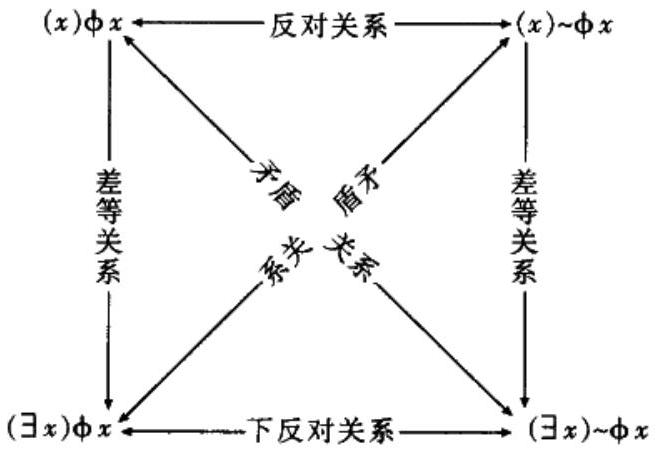
\includegraphics[max width=\textwidth, center]{2025_05_15_6a28331d5e7c993ad07ag-463}

图10—1\\
继续假定至少存在一个个体,就该方阵我们可以说:\\
1.顶端的两个命题是反对关系;就是说,它们可以同时为假,但不能同时为真。

2.底端的两个命题是下反对关系;就是说,它们可以同时为真,但不能同时为假。

3.对角线相反两端的命题是矛盾关系;它们中一个为真,则另一个必定为假。

4.在方阵的每侧,下面命题的真被它正上方命题的真所蕴涵。

\section*{10.3 传统主一谓命题}
运用存在和全称量词,以及根据对图 10-1 中对当方阵的理解,我们现在开始分析(并且在推理中准确地使用)以下四种为传统逻辑研究所注重的普遍命题。这四种命题的标准例子如下:

\begin{center}
\begin{tabular}{ll}
所有人是有死的。 & [全称肯定:A] \\
所有人都不是有死的。 & [全称否定:E] \\
有些人是有死的。 & [特称肯定:I] \\
有些人不是有死的。 & [特称否定:O] \\
\end{tabular}
\end{center}

每种命题通常由其字母来指称:两种肯定命题用 A 和 I(来自拉丁文\\
affirmo,我肯定);两种否定命题用 E 和 O (来自拉丁文 nego,我否认)。 ${ }^{[4]}$

用量词符号化这些命题,使得我们进一步扩大了命题函项概念。首先来看 A 命题"所有人是有死的",我们从下述命题开始逐次解释:

给定不管任何事物,如果它是人,它是有死的。

其中关系代词"它"的两次出现显然是回指它们共同的先行词"事物"。与上节的前部分一样,因为它们有同样的(不确定的)指称,从而都能用字母"$x$"替换。于是该命题可改写成:

给定任何 $x$ ,如果 $x$ 是人,那么 $x$ 是有死的。

现在,用先前引入的"如果一那么"的符号,可以把前一个命题改写成:

给定任何 $x, x$ 是人 $\supset x$ 是有死的。

最后,用我们已掌握的命题函项符号和量词,原来的 A 命题可表示为:

$$
(x)(H x \supset M x)
$$

在我们的符号翻译中, A 命题是以一种新的命题函项的全称量化形式出现的。表述式 $H x \supset M x$ 是一个命题函项,它既没有单称肯定命题又没有单称否定命题作为其代人例,而是以条件陈述作为代人例,这些条件陈述的前件和后件是具有同样主项的单称命题。命题函项 $H x \supset M x$ 的代人例有条件陈述 $H a \supset M a 、 H b \supset M b 、 H c \supset M c 、 H d \supset$ $M d$ 等等。

另一些命题函项则以有同样主项的单称命题的合取为代入例。例如, $H a \cdot M a 、 H b \cdot M b 、 H c \cdot M c 、 H d \cdot M d$ 等等都是命题函项 $H x \cdot M x$ 的代人例。还有一些形如 $W x \vee B x$ 的命题函项,它们的代入例是诸如 $W a \vee$ $B a$ 和 $W b \vee B b$ 这样的析取式。实际上,任何以具有相同主项的单称命题为分支陈述的真值函项复合命题,都可以看做由某些或所有真值函项联结词(圆点号、楔劈号、马蹄号、三杠等值号和波浪号)加之简单谓词\\
( $A x 、 B x 、 C x 、 D x \cdots \cdots$ )所构成的命题函项的代人例。在把 A 命题翻译成( x )( $H \mathrm{x} \supset M x$ )时,圆括号充当标点符号,用以表明全称量词( $x$ ) "作用于"整个(复合)命题函项 $H x \supset M x$ ,或命题函项 $H x \supset M x$"作为其辖域"。

在继续讨论直言命题的其他传统形式之前,应该注意符号公式( $x$ ) ( $H x \supset M x$ )不仅是对标准形式的命题"所有 $H$'s 都是 $M$'s"的翻译,而且是对任何一个有同样含义的自然语言句子的翻译。 ${ }^{[5]}$ 在自然语言中,述说这同一件事有许多不同的方式。它们的部分清单如下:"$H$ 是 $M$","一个 $H$ 就是一个 $M$","每个 $H$ 是 $M$","每一个 $H$ 是 $M$","任何 $H$ 是 $M$", "没有 $H$ 不是 $M$","是 $H$ 的每个事物都是 $M$","是 $H$ 的任何事物都是 $M "$ ,"如果任何事物是 $H$ ,那么它是 $M$","如果某事物是 $H$ ,那么它是 $M$","是 $H$ 的无论什么东西都是 $M$","$H$'$s$ 全都是 $M$'$s$","只有 $M$'$s$ 是 $H^{\prime} s "$ ,"除了 $M^{\prime} s$ 以外,没什么是 $H^{\prime} s "$ ,"没什么是 $H$ ,除非它是 $M^{\prime}$",以及"没有什么是 $H$ 但不是 $M$"。再者,同一含义的命题可以用抽象名词表达:"人蕴涵(或涵衍)有死"可以正确地符号化为一个 A 命题。符号逻辑语言对相当数量的自然语言句子的共同含义有一个单一的表达式,这一点被认为是符号逻辑在认知或信息方面比自然语言优越之处,一一尽管从修辞力或诗意表现的观点看,我们承认这是一种劣势。 E 命题"所有人都不是有死的"可以被依次释为:

\begin{displayquote}
给定不管任何个体事物,如果它是人,那么它不是有死的。\\
给定任何 $x$ ,如果 $x$ 是人,那么 $x$ 不是有死的。\\
给定任何 $x, x$ 是人 $\supset x$ 不是有死的。
\end{displayquote}

最后可以释为:

$$
(x)(H x \supset \sim M x)
$$

这种符号翻译不仅表示了自然语言中传统的 E 形式,同样也表示了一些说同一件事的不同方式,如"没有是 $M$ 的 $H$","没有什么既是 $H$ 又是 $M$",以及"$H$ 从不是 $M$"。

同样,I命题"有些人是有死的"可以依次释为:

至少有一个是人且有死的事物。\\
至少有这样一个 $x, x$ 是人并且 $x$ 是有死的。\\
至少有这样一个 $x, x$ 是人• $x$ 是有死的。

进而可以释为:

$$
[(\exists x)(H x \cdot M x)]
$$

最后, O 命题"有些人不是有死的"可以依次释为:

至少存在一个是人但不是有死的事物。\\
至少存在这样一个 $x, x$ 是人并且 $x$ 不是有死的。\\
至少存在这样一个 $x, x$ 是人• $\sim x$ 是有死的。

它可以完全符号化为:

$$
[(\exists x)(H x \cdot \sim M x)]
$$

若用希腊字母 phi( $\phi$ )和 psi( $\Psi$ )表示任何一个谓词,传统逻辑的四个主—谓型普遍命题可以在图 10—2 所示的方阵中得到表达。\\
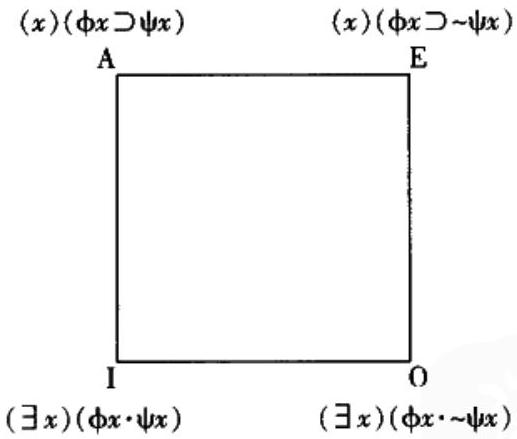
\includegraphics[max width=\textwidth, center]{2025_05_15_6a28331d5e7c993ad07ag-466}

图10-2\\
显然, A 命题和 O 命题是矛盾关系,一个是另一个的否定; E 命题和 I 命题也是矛盾关系。

有人可能会认为,一个 I 命题可以从与之相对的 A 命题推出,一个 O命题可以从与之相对的 E 命题推出,但情况并非如此。一个 A 命题为真时,与之对应的 I 命题却可能是假的。如果 $\phi_{x}$ 是一个没有真代人例的命

题函项,那么,不管命题函项 $\Psi x$ 有何种代人例,(复合)命题函项 $\phi_{x} \supset$ $\Psi x$ 的全称量化式都是真的。例如,考虑命题函项"$x$ 是一个人首马身的怪物",我们把它简写为 $C x$ 。因为不存在人首马身的怪物,$C x$ 的每个代入例都是假的,即 $C a 、 C b 、 C c \cdots \cdots$ 都为假。因此,复合命题函项 $C x \supset B x$的每个代人例都是一个前件为假的条件陈述。这样,其代人例 $\mathrm{Ca} \supset \mathrm{Ba}$ 、 $C b \supset B b 、 C c \supset B c$ 都是真的,因为任何一个断言实质蕴涵的条件陈述,如果其前件为假,那么它必定为真。由于其所有代人例都是真的,所以,命题函项 $C x \supset B x$ 的全称量化式为真,即 A 命题 $(x)(C x \supset B x)$ 为真。但与之相对的 I 命题 $(\exists x)(C x \cdot B x)$ 却是假的,因为命题函项 $C x \cdot B x$没有真代人例。 $C x \cdot B x$ 没有真代人例可以从 $C x$ 没有真代人例推出。 $C x \cdot B x$ 的各个代人例,如 $C a \cdot B a 、 C b \cdot B b 、 C c \cdot B c \cdots \cdots$ 都是第一个合取支为假的合取式,因为 $C a 、 C b 、 C c \cdots \cdots$ 都为假。由于其所有代人例都为假,所以命题函项 $C x \cdot B x$ 的存在量化式为假,即 I 命题( $\exists x$ )( $C x \cdot B x$ )为假。因此,有可能一个 A 命题是真的,而与之对应的 I 命题却是假的。

这种分析还可表明,为什么有可能一个 E 命题是真的,而与之对应的 $O$ 命题却是假的。如果我们以命题函项 $\sim B x$ 替换前面讨论中的命题函项 $B x$ ,那么,$(x)(C x \supset \sim B x)$ 可以是真的,而 $(\exists x)(C x \cdot \sim B x)$ 却是假的。当然,这也是因为并没有人首马身的怪物。

问题的关键在于:A 命题和 E 命题并不断言或假定任何事物存在,它们仅断言情况是这样的:如果有某事,则有另外一件事。但 I 命题和 O 命题却假定某物存在,它们断言情形是这样的:有这件事并且有另一件事。 1 命题和 $O$ 命题中的存在量词是区别的关键所在。从一个并不断言或假定任何事物存在的命题推出某物的存在,这显然是错误的。

如果我们假定至少有一个个体存在,那么( $x$ )( $C x \supset B x$ )确实蕴涵 ( $\exists x) ~(C x \supset B x)$ 。但后者不是一个 I 命题。 I 命题"有些人首马身的怪物是漂亮的"应符号化为 $(\exists x)(C x \cdot B x)$ ,它说的是,至少存在一个漂亮的人首马身的怪物。但在自然语言中,被符号化为( $\exists x$ )( $C x \supset B x$ )的东西,可以被理解为"至少存在一个如此这般的事物,如果它是人首马身的怪物,那么它是漂亮的"。它并没说存在一个人首马身的怪物,而只是说存在一个个体,它或者不是人首马身的怪物,或者是漂亮的。而这个命题只在两种情况下是假的:第一,如果根本不存在个体;第二,如果所有个体都是人首马身的怪物,并且它们当中没有一个是漂亮的。通过作这样

一个明确的(并且显然是真的)假定,即假定宇宙中至少存在一个个体,我们可以排除第一种情形。第二种情形是如此极端地不合理,以致与 I 形命题( $\exists x$ )( $\phi_{x} \cdot \Psi x$ )的重要性相反,任何形如( $\exists x$ )( $\phi_{x} \supset \Psi x$ )的命题都必定是非常平庸的。显而易见,尽管在自然语言中 A 命题"所有人是有死的"和 I 命题"有些人是有死的"的区别,仅在于初始词"所有"和"有些"的不同,但它们意义上的区别并不限于全称量化和存在量化,而是比这深刻得多。经量化而产生 A 命题和 I 命题的命题函项不仅在量化上有区别,而且它们还是不同的命题函项,一个含有"$\supset$",另一个含有"•"。换言之,A 命题和 I 命题并不像它们在自然语言中看起来那么相似。它们之间的区别可通过使用命题函项符号和量词符号得以彰显。

就逻辑操作来说,处理那些否定号的出现——如果有否定号出现的话——只作用于简单谓述的公式最为方便。因此,我们将在必要时通过替换来得到这种公式。要做到这一点很简单。从第9章所确立的推论规则可知,我们可以用另一个与之逻辑等价的表述式来替换一个表述式。而我们有四个这样的逻辑等价式(10.2节),它们当中否定号在量词之前的命题,都与另一个否定号直接作用于简单谓述的命题等价。用我们熟悉已久的推论规则,可以移动否定号,使它们最终不再作用于复合表达式,而只作用于简单谓述。譬如说,公式:

$$
\sim(\exists x)(F x \cdot \sim G x)
$$

可以依次改写。首先,如果我们用 10.2 节所给的第三个逻辑等价式,它可以变形为:

$$
(x) \sim(F x \cdot \sim G x)
$$

然后,可运用德摩根律使之变成:

$$
(x)(\sim F x \vee \sim \sim G x)
$$

再用双重否定律可得公式:

$$
(x)(\sim F x \vee G x)
$$

最后,若援引实质蕴涵定义,原公式也可以改写成下述 A 命题:

$$
(x)(F x \supset G x)
$$

在转到关于非复合陈述推论的话题之前,读者应该进行一些把非复合陈述从自然语言翻译成逻辑符号的训练。自然语言有如此之多不规则的和惯用的构造,以致不可能有把自然语言语句翻译成逻辑符号的简单规则。在任何情形下都要先理解语句的含义,然后用命题函项和量词术语予以重述。

\section*{练习题}
I.用所提示的缩写,把下述每个都翻译成量词和命题函项的逻辑符号,并使每个公式都以量词而不是否定号开头。

\section*{例题}
1.没有畜生是没有一点同情心的。( $B x: ~ x$ 是畜生;$P x: ~ x$ 是有同情心的。)

\section*{解答 $(x)(B x \supset P x)$}
2.麻雀不是哺乳动物。( $S x: x$ 是麻雀;$M x: x$ 是哺乳动物。)\\
3.记者在场。( $R x: x$ 是记者;$P x: x$ 在场。)\\
4.护士总是很体贴。( $N x: x$ 是护士;$C x: x$ 很体贴。)\\
*5.外交家并非都富有。( $D x: x$ 是外交家;$R x: x$ 富有。)\\
6.大使总是有威严的。( $A x: ~ x$ 是大使;$D x: ~ x$ 是有威严的。)\\
7.所有的童子军都不骗人。( $B x: ~ x$ 是童子军;$C x: ~ x$ 骗人。)\\
8.只有拿到执业资格证的内科医师才能负责医疗。( $L x: x$ 是拿到执业资格证书的内科医师;$C x: ~ x$ 能负责医疗。)

9.蛇毒有时是致命的。( $S x: x$ 是蛇毒;$F x: x$ 是致命的。)\\
*10.感冒从不是致命的。( $C x: x$ 是感冒;$F x: x$ 是致命的。)\\
11.一个小孩用手指着那个皇帝。 $(C x: x$ 是小孩;$P x: x$ 用手指着那个皇帝。)

12.并非所有的小孩都用他们的手指着那个皇帝。( $C x: ~ x$ 是小孩; $P x$ :$x$ 用手指着那个皇帝。)

13.闪光的不都是金子。( $G x: x$ 闪光;$G x: x$ 是金子。)\\
14.只有勇敢者才应配美人。( $B x: ~ x$ 是勇敢的;$D x: ~ x$ 应配美人。)\\
*15.只有美国公民才能在美国选举中投票。( $C x: ~ x$ 是美国公民;$V x$ : $x$ 能在美国选举中投票。)

16.美国的公民只能在美国的选举中投票。( $E x: ~ x$ 是美国公民能投

票的选举;Ux:$x$ 是美国选举。)\\
17.并非每个求职者都被聘用。( $A x: x$ 是求职者;$H x: x$ 被聘用。)\\
18.没有任何一个求职者被聘用。( $A x: x$ 是求职者;$H x: x$ 被聘用。)

19.没有什么重要的事情被谈论。( $L x: x$ 是重要的事情;$S x: x$ 被谈论。)\\
-20.乐于助人的人有权进行批评。( $C x: ~ x$ 有权进行批评;$H x: ~ x$ 是乐于助人的人。)

II.把下列句子翻译成命题函项和量词构成的逻辑记法,每种情形下公式都以量词而不是否定号开头。\\
*1.除非通过计算,否则在战争中没有什么东西是可以实现的。\\
--Napoleon Bonaparte\\
2.没有人不相信自然律。\\
-Donna Haraway,The Chronicle of Higher Education, 28 June 1996

3.每天都重新战胜自己的人会获得自由与生存。\\
— Johann Wolfgang Von Goethe,Faust, Part II

4.没有谁是彻底悲惨的,除非他被判住在爱尔兰。\\
—Jonathan Swift\\
*5.并非每个好事物都是安全的,并非每个危险事物都是坏的。\\
-David Brooks,in The Weekly Standard, 18 August 1997

6.没有我们不能改善的东西。\\
--Advertising slogan,Ernst and Young,Ac- countants

7.提得好的问题就已解决了一半。\\
-Charles Kettering,former Research Di- rect for General Motors

8.没有一个后来变坏的女巫或男巫不是从斯莱特林出来的。\\
-J.K.Rowling,in Harry Potter and the Sorcerer's Stone

9.每个人都会不喜欢某些东西,但没有人不喜欢维列•尼尔森。\\
*10.除了俊子,没人不是为了钱而写作。\\
-Samuel Johnson\\
III.给下面的每个公式找一个与之逻辑等价的范型公式。\\
*1.~$(x)(A x \supset B x)$\\
2.$\sim(x)(C x \supset \sim D x)$\\
3.$\sim(\exists x)(E x \cdot F x)$\\
4.$\sim(\exists x)(G x \cdot \sim H x)$\\
*5.$\sim(x)(\sim I x \vee J x)$\\
6.$\sim(x)(\sim K x \vee \sim L x)$\\
7.$\sim(\exists x)[\sim(M x \vee N x)]$\\
8.$\sim(\exists x)[\sim(O x \vee \sim P x)]$\\
9.$\sim(\exists x)[\sim(\sim Q x \vee R x)]$\\
10.$\sim(x)\left[\sim\left(S_{x} \cdot \sim T x\right)\right]$\\
11.$\sim(x)[\sim(\sim U x \cdot \sim V x)]$\\
12.$\sim(\exists x)[\sim(\sim W x \vee X x)]$

\section*{10.4 有效性证明}
某些论证的有效性取决于在其中出现的非复合陈述的内在结构,为了构造它们有效性的形式证明,我们必须进一步扩充推论规则表。只需增加四个规则,我们将在涉及必须使用它们的那些论证时逐次引人。

考虑本章所引的第一个论证:"所有人都是有死的。苏格拉底是人。因此,苏格拉底是有死的。"可以符号化为:

$$
(x)(H x \supset M x)
$$

Hs\\
$\therefore M s$\\
第一个前提断定了命题函项 $H x \supset M x$ 的全称量化式。由于一个命题函项的全称量化式为真,当且仅当它的所有代人例都为真,从第一个前提可以推出命题函项 $H x \supset M x$ 的任何一个我们需要的代人例。此处即可以推出代人例 $H s \supset M s$ 。从它和第二个前提 $H s$ ,根据肯定前件式,可以直接得出结论 $M s$ 。

如果给我们的推论规则表加上这样一个原则,即一个命题函项的任一代入例都可以有效地从其全称量化式推得,那么,依照扩充了的基本有效论证形式表,我们可以给出该论证之有效性的形式证明。这种新的推论规则就是全称列举原则 ${ }^{[6]}$ ,简写为"UI"。用希腊字母 $n u(v)$ 表示任一个体符号,我们可以把该新规则表述为:

$$
\begin{aligned}
& \mathrm{UI}:(x)(\phi x) \\
& \quad \therefore \phi v \quad(v \text { 是任一个体符号 })
\end{aligned}
$$

其有效性的形式证明现在可以写成:

\begin{center}
\begin{tabular}{ll}
1.$(x)(H x \supset M x)$ &  \\
2.$H s$ &  \\
 & $\therefore M s$ \\
3.$H s \supset M s$ & $1, \mathrm{UI}$ \\
4.$M s$ & $3,2, \mathrm{M} . \mathrm{P}$. \\
\end{tabular}
\end{center}

增加 UI 大大地强化了我们的证明工具,但我们还需要更多的规则。需要另一些支配量化的规则,这种需要是和这样的论证相联系的,如"所有人都是有死的。所有希腊人都是人。因此所有希腊人都是有死的。"这个论证的符号翻译是:

$$
\begin{aligned}
& (x)(H x \supset M x) \\
& (x)(G x \supset H x) \\
& \therefore(x)(G x \supset M x)
\end{aligned}
$$

其中,前提和结论都是普遍命题而不是单称命题,是命题函项的全称量化式而不是其代人例。根据 UI,我们可以有效地从这两个前提推出下述条件陈述对子:

$$
\begin{array}{lllll}
G a \supset H a & G b \supset H b & G c \supset H c & G d \supset H d & \\
H a \supset M a & H b \supset M b & H c \supset M c & H d \supset M d & \ldots \ldots
\end{array}
$$

通过连续使用假言三段论规则,我们可以有效地推出结论:

$$
G a \supset M a, \quad G b \supset M b, \quad G c \supset M c, \quad G d \supset M d \quad \ldots \ldots
$$

如果 $a, b, c, d \cdots \cdots$ 是所有存在的个体,那么,我们从前提的真就可以有效地推出命题函项 $G x \supset M x$ 的所有代人例的真。由于一个命题函项的全称量化式为真,当且仅当,它的所有代人例都为真,我们可以继续推出 ( $x$ )( $G x \supset M x$ )为真,而它就是该论证的结论。

前面一段可以看做构成了上述论证有效性的一个非形式的证明,在证明中运用了假言三段论规则和支配量化的两个规则。它描述了一个长度不确定的陈述序列:前提中两个被全称量化的命题函项的所有代人例的序

列,以及其全称量化式是结论的那个命题函项的所有代人例的序列。一个形式证明不能包含这样的不确定的甚或无限长的陈述序列。因此,必须寻求某种方法,它能以某种有限的、确定的方式来表达这些长度不确定的序列。

基础数学的一个一般技巧为做到这一点提供了提示。一个试图证明所有三角形都具有某种属性的几何学者,可以从"令 $A B C$ 是一个任意选取的三角形"出发。然后对三角形 $A B C$ 进行推理,确立它具有被探究的那种属性,由此可得出结论,所有三角形具有该属性。是什么东西能为他的最后结论进行辩护呢?承认这个特定的三角形 $A B C$ 有该属性,为什么可以得出所有的三角形都有这种属性?答案很容易见得:如果除了假定它是三角形外,我们对三角形 $A B C$ 没作任何其他假定,那么,符号"$A B C$"可以被看做是指称你所挑选的任何三角形。几何学者的论证确立了任一三角形具有所探究的属性,而如果任一三角形都具有某属性,那么所有的三角形都具有该属性。我们现在也可引进一个符号,它类似于几何学者所谈论的"一任意选取的三角形 $A B C$"。这使我们可以谈论某命题函项的任一代人例,而不用去罗列其不确定的或无限数量的代人例。

我们将用(迄今还没用过)小写字母 $y$ 来指称一任意选取的个体,以一种类似于几何学者使用字母 $A B C$ 的方式来使用它。由于从一个命题函项的全称量化式可以推出它的任一代人例,故亦可推出以 $y$ 替换 $x$ 所得到的那个代人例。在此,$y$ 指称"一任意选取的"个体。这样,我们可以着手进行上述论证有效性的形式证明:

1.$(x)(H x \supset M x)$\\
2.$(x)(G x \supset H x)$

$$
\therefore(x)(G x \supset M x)
$$

\begin{center}
\begin{tabular}{ll}
3.$H y \supset M y$ & 1, UI \\
4.$G y \supset H y$ & 2, UI \\
5.$G y \supset M y$ & 4,3, H.S. \\
\end{tabular}
\end{center}

我们从前提演绎出了陈述 $G y \supset M y$ ,由于 $y$ 指称"一任意选取的个体",所以,该陈述实际上是断言命题函项 $G x \supset M x$ 的任一代人例为真。既然任一代人例为真,所有的代人例必定为真,因此,该命题函项的全称量化也必是真的。我们可以把这个原则加到推论规则表中,表述如下:从一个

命题函项关于任意选取的个体名称的代入例,我们可以有效地推出该命题函项的全称量化式。这个规则允许我们进行概括,也就是从一个特定的代人例进到一个概括的或全称量化的表述式,故称为全称概括原则,并缩写为"UG"。它被表述成:

$$
\begin{aligned}
\mathrm{UG}: & \phi_{y} \\
\therefore(x)\left(\phi_{x}\right) & (y \text { 指称"一任意选取的个体") }
\end{aligned}
$$

前面的形式证明的第六行即最后一行,现在就可以写(并被证明)为:\\
6.$(x)(G x \supset M x)$\\
5,UG

我们来回顾一下前面的讨论。在几何学者的证明中,对 ABC 所作的唯一假定就是它是一个三角形,因此,被证明为对 ABC 为真的东西也就被证明为对任一三角形为真。在我们的证明中,对 $y$ 所作的唯一假定是它是一个个体词,因此,被证明为对 $y$ 为真的东西也就被证明为对任一个体为真。符号 $y$ 是一个个体符号,但它是一个很特殊的个体符号。特别是通过使用 UI,它被引人到证明中,并且只有当出现了 $y$ 时才允许使用UG。

以下是另一个有效论证,它的有效性的证明要求使用 UG 和 UI:"没有人是完美的。所有希腊人都是人。因此没有希腊人是完美的。"${ }^{[7]}$ 它的有效性的形式证明是:

1.$(x)(H x \supset \sim P x)$\\
2.$(x)(G x \supset H x)$

$$
\therefore(x)(G x \supset \sim P x)
$$

3. $\mathrm{H} y \supset \sim \mathrm{P} y \quad 1$ ,UI\\
4.GyつHy 2,UI\\
5.Gyコ~Py 4,3,H.S.\\
6.$(x)(G x \supset \sim P x) \quad$ 5,UG\\
上面的证明看起来多少有点不自然,需要我们对 $(x)\left(\phi_{x}\right)$ 和 $\phi_{y}$ 做出仔细的区分。说它们尽管不同但根据 UG 和 UI 又必定可以相互推出,似乎二者之间没有实质差别。但它们之间确实有一种形式的差别。陈述 ( $x$ )( $H x \supset M x$ )是一个非复合陈述,而 $H y \supset M y$ 作为一个条件陈述,是一个复合陈述。依照原先含有 19 个规则的推论规则表,从两个非复合陈述 $(x)(G x \supset H x)$ 和 $(x)(H x \supset M x)$ 出发,我们不能作相关的推理。

但从复合陈述 $G y \supset H y$ 和 $H y \supset M y$ 出发,根据假言三段论,就可以得出所要的结论 $G y \supset M y$ 。规则 $U I$ 用来从非复合陈述得出复合陈述,我们先前的推论规则无法施于非复合陈述,但可以施于复合陈述以得出想要的结论。因此,量化规则增加了我们的逻辑工具,使得我们能够证明本质地涉及非复合(概括的)命题的论证的有效性,以及前一些章节所讨论的另一类(更简单的)论证的有效性。另一方面,尽管有这种形式的差别,( $x$ ) ( $\phi_{x}$ )和 $\phi_{y}$ 必定是逻辑等价的,否则,规则 UG 和 UI 就不是有效的。对依据推论规则表来证明论证的有效性来说,这种差别和逻辑等价都很重要。把 UG 和 UI 加到推论规则表中使之得到了很大强化。

当我们转向涉及存在命题的论证时,推论规则表必须进一步扩充。我们可从这样一个很便捷的例子着手:"所有罪犯都是邪恶的。有些人是罪犯。因此有些人是邪恶的。"它可以符号化为:

$$
\begin{aligned}
& (x)(C x \supset V x) \\
& (\exists x)(H x \cdot C x) \\
& \therefore(\exists x)(H x \cdot V x)
\end{aligned}
$$

一个命题函项的存在量化式为真,当且仅当,它至少有一个真代人例。因此,无论 $\phi$ 指谓何种属性,( $\exists x$ )( $\phi_{x}$ )所说的就是,至少存在一个具有属性 $\phi$ 的个体。如果一个个体常元(除了特定的符号 $y$ )在早先的上下文中没有使用过,我们可以用它来指称具有属性 $\phi$ 的那个个体,或者,如果有几个具有属性 $\phi$ 的个体,用它指称其中的某一个。若知道存在这样一个个体,臂如 $a$ ,我们就知道 $\phi_{a}$ 是命题函项 $\phi_{x}$ 的一个真代人例。故我们给推论规则表加上这样一个规则:从一个命题函项的存在量化式,可以推得关于在其语境中早先没有出现过的任一个体常元(除 $y$ 之外)的代入例。这个新推论规则叫存在列举原则,可缩写为"EI"。它可以表述成:

$$
\mathrm{EI}:(\exists x)\left(\phi_{x}\right)
$$

$\therefore \phi U \quad[U$ 是任一在语境中先前没有出现过的个体常元(除 $y$之外)〕

如果确认所添加的推理规则 EI,我们即可着手证明上述论证的有效性:

1.$(x)(C x \supset V x)$

2.$(\exists x)(H x \cdot C x)$

$$
\therefore(\exists x)(H x \cdot V x)
$$

3. $\mathrm{Ha} \cdot \mathrm{Ca}$ 2,EI\\
4. $\mathrm{Ca} \supset \mathrm{Va} \quad 1$ ,UI\\
5. $\mathrm{Ca} \cdot \mathrm{Ha}$ 3,Com.\\
6. Ca 5,Simp.\\
7.Va 4,6,M.P.\\
8. Ha 3 ,Simp.\\
9. $\mathrm{Ha} \cdot \mathrm{Va} \quad 8,7$, Conj.\\
到目前为止,我们演绎出了 $\mathrm{Ha} \cdot \mathrm{Va}$ ,它是其存在量化式被结论所断 40 s定的那个命题函项的代人例。由于一个命题函项的存在量化式为真,当且仅当,它至少有一个为真的代人例,我们为推论规则表再增加这样一个规则:从一个命题函项的任一为真的代入例,我们可以有效地推出该命题函项的存在量化式。这第四个也是最后一个推论规则叫存在概括原则,缩写为"EG",它可以表述为:

$$
\begin{gathered}
\text { EG: } \phi_{v} \quad(v \text { 是任一个体符号) } \\
\therefore(\exists x)\left(\phi_{x}\right)
\end{gathered}
$$

前面开始的那个证明的第十行也即最后一行,现在可以写(并且被证明)为:

$$
\text { 10. }(\exists x)(H x \cdot V x) \quad 9, \mathrm{EG}
$$

对 EI 的使用必须施加必要的限制,这一点可以通过考察如下明显无效的论证看出来:"有些短伆鳄被关在笼子里。有些鸟被关在笼子里。因此有些短吻鳄是鸟。"如果我们不对 EI 施加这样一种限制——根据 EI 从一个命题函项的存在量化式推出的代人例,只能含有一个在语境中早先没出现过的个体符号(除 $y$ 之外),那么,我们就可以构造出这个无效论证的有效性"证明"。这样一个错误的"证明"可以如下进行:

1.$(\exists x)(A x \cdot C x)$\\
2.$(\exists x)(B x \cdot C x)$

$$
\therefore(\exists x)(A x \cdot B x)
$$

4. $\mathrm{Ba} \cdot \mathrm{Ca}$\\
5.$A a$\\
6.$B a$\\
7.$A a \cdot B a$\\
8.$(\exists x)(A x \cdot B x)$

2,EI(错!)\\
3,Simp.\\
4,Simp.\\
5,6,Conj.\\
7,EG

这个"证明"的错误出现在第 4 行。我们从第二个前提 $(\exists x)(B x \cdot C x)$可知,至少存在这样一个事物,它既是鸟又被关在笼子里。如果我们在第 4 行给它自由地指派一个名称 $a$ ,我们当然就可以断言 $B a \cdot C a$ 。但我们绝不能自由地指派这样一个"$a$",因为它作为一只关在笼子里的短吻鳄的名字,已经先在第 3 行中出现了。为避免这种错误,我们使用 EI 时必须服从这种必要的限制。由前面的讨论可明显见得:在任何要使用 EI 和 UI 的证明中,应该总是先使用 EI 。

对更复杂的论证模式来说,特别是那些涉及关系的论证,我们还必须对四个量化规则施加某些附加限制。但就目前这种类型的论证即传统上叫做直言三段论的论证来说,目前的限制已足以避免出错。

\section*{四个附加推论规则}
下述四个规则使得我们可以把非复合的、概括的命题转化为与其等值的复合命题,第 9 章所列的那 19 个推论规则适用于这些复合命题。它们还使我们可以把复合命题转化为等值的非复合命题。因此,这四个附加规则使得构造某些论证的有效性的形式证明成为可能,这些论证的有效性取决于它们所包含的一些非复合陈述的内在结构。这四个附加规则如下:

\section*{1.全称列举}
UI:$(x)(\phi x), \therefore \phi \cup$(在此,$v$ 是任一个体符号)\\
这个规则大体上说的是:一个命题函项的任何代入例都可以从它的全称量化式推出。

\section*{2.全称概括}
UG:$\phi_{y}, \therefore(x)\left(\phi_{x}\right)$(在此,$y$ 指称"一任意选取的个体")\\
这个规则大体上说的是:从一个命题函项关于一任意选取的个体名称的代入例,我们可以有效地推出该命题函项的全称量化式。

\section*{3.存在列举}
EI:$(\exists \mathrm{x})\left(\phi_{\mathrm{x}}\right), \therefore \phi_{\mathrm{u}}$[在此,$v$ 是任一在上下文中先前没有出现

过的个体常元(除了 y)〕\\
这个规则大体上说的是:从一个命题函项的存在量化式,我们可以推出,它关于早先上下文的任何地方都没出现的任一个体常元(除了 $y) ~$ 的代入例为真。

\section*{4.存在概括}
EG:$\phi_{v}, \therefore(\exists x)\left(\phi_{x}\right)$(在此,$v$ 是任一个体符号)\\
这个规则大体上说的是:从一个命题函项的任一为真的代入例,我们可以有效地推出该命题函项的存在量化式。

\section*{练习题}
I.为下述每个论证构造一个有效性的形式证明。

\section*{例题}
1.$(x)(A x \supset \sim B x)$\\
$(\exists x)(C x \cdot A x)$\\
$\therefore(\exists x)(C x \cdot \sim B x)$

\section*{解答}
这个论证的结论是一个存在量化陈述。因此,最后一步显然要用 EG (存在概括)。为了得到所要的那一行,我们首先必须对前提实施列举,即把 EI(存在列举)运用到第二个前提,把 UI(全称列举)运用到第一个前提。使用 EI 时的限制使得这一点是根本性的,即必须在运用 UI 之前运用 EI,这样我们就可以对这两者都使用同样的个体常元,譬如 $a$ 。证明如下:

1.$(x)(A x \supset \sim B x)$\\
2.$(\exists x)(C x \cdot A x)$

$$
\therefore(\exists x)(C x \cdot \sim B x)
$$

3. $\mathrm{Ca} \cdot \mathrm{Aa}$ 2,EI\\
4. $\mathrm{Aa} \supset \sim \mathrm{Ba} \quad 1$ ,UI\\
5. $\mathrm{Aa} \cdot \mathrm{Ca}$ 3,Com.\\
6. Aa 5,Simp.\\
7.$\sim B a$\\
4,6,M.P

8.$C a$\\
9. $\mathrm{Ca} \cdot \sim \mathrm{Ba}$\\
10.$(\exists x)(C x \cdot \sim B x)$

3,Simp.\\
8,7,Conj.\\
9,EG\\
2.\\
( $x$ )$(D x \supset \sim E x)$\\
3.$(x)(G x \supset H x)$\\
( $x$ )$(F x \supset E x)$\\
$\therefore(x)(F x \supset \sim D x)$\\
( $x$ )$(I x \supset \sim H x)$\\
$\therefore(x)(I x \supset \sim G x)$

4.$(\exists x)(J x \cdot K x)$\\
-5.( $x$ )( $M x \supset N x$ )\\
( $x$ )( $J x \supset L x$ )\\
$(\exists x)(M x \cdot O x)$\\
$\therefore(\exists x)(L x \cdot K x)$\\
$\therefore(\exists x)(O x \cdot N x)$\\
6.$(\exists x)(P x \cdot \sim Q x)$\\
7.$(x)(S x \supset \sim T x)$\\
( $x$ )$(P x \supset R x)$\\
( $\exists x$ )( $S x \cdot U x$ )\\
$\therefore(\exists x)(R x \cdot \sim Q x)$\\
$\therefore(\exists x)(U x \cdot \sim T x)$\\
8.$(x)(V x \supset W x)$\\
9.$(\exists x)(Y x \cdot Z x)$\\
( $x$ )( $W x \supset \sim X x$ )\\
( $x$ )$(Z x \supset A x)$\\
$\therefore(x)(X x \supset \sim V x)$\\
$\therefore(\exists x)(A x \cdot Y x)$\\
-10.( $x$ )( $B x \supset \sim C x$ )\\
11.$(x)(F x \supset G x)$\\
$(\exists x)(C x \cdot D x)$\\
( $\exists x$ )( $F x \cdot \sim G x$ )\\
$\therefore(\exists x)(D x \cdot \sim B x)$\\
$\therefore(\exists x)(G x \cdot \sim F x)$\\
II.用所给符号,为下述每个论证构造一个有效性的形式证明。\\
*1.没有运动员是书呆子。卡罗尔是书呆子。因此卡罗尔不是运动员。 ( $A x, B x, c$ )

2.所有舞蹈演员都是精力旺盛的。有些击剑者不是精力旺盛的。因此,有些击剑者不是舞蹈演员。( $D x, E x, F x$ )

3.没有赌徒是幸福的。有些理想主义者是幸福的。因此,有些理想主义者不是赌徒。 $(G x, H x, I x)$

4.所有小丑都是流讯。没有流讯是幸运的。因此,没有小丑是幸运的。( $J x, K x, L x$ )\\
*5.所有山民都是友好的。有些歹徒是山民。因此,有些歹徒是友好的。 $(M x, N x, O x)$

6.只有和平主义者是教友派信徒。有一些虔诚的教友派信徒。因此,和平主义者有些是虔诚的。( $P x, Q x, R x$ )

7.诈骗者都是贼。除了穷困的人,没人是贼。因此,诈骗者都是穷

困的人。( $S x, T x, U x$ )\\
8.没有小提琴家不是富有的。没有富有的木琴演奏家。因此,小提琴家绝不是木琴演奏家。( $V x, W x, X x$ )

9.除了勇敢者外,没人配得上美人。只有战士是勇敢者。因此,只有战士配得上美人。( $D x: ~ x$ 配得上美人;$B x: ~ x$ 是勇敢者;$S x: ~ x$ 是战士)\\
${ }^{*}$ 10.每个有所求的人都有所得。西蒙无所得。因此,西蒙无所求。 ( $A x, R x, s$ )

11.安妮:没有哪个畜生如此凶残却又有点同情心。\\
格洛斯特:但我一点同情心也没有,因此,我不是畜生。( $B x$ , Px,g)\\
-William Shakespeare,Richard the Third, act 1 ,sc. 2

\section*{10.5 无效性证明}
要证明一个涉及量词的论证无效,我们可以用逻辑类推进行反驳的方法。例如:"所有保守派都是行政机关的反对者;有些代表是行政机关的反对者;因此,有些代表是保守派。"这个论证可以通过这样一个逻辑类推被证明为无效,即"所有猫都是动物;有些狗是动物;因此,有些狗是猫"。这个论证显然无效,因为已知它的前提为真而结论为假。但这种类比并非总是很容易构造。因此,需要某种更有力的证明无效性的方法。

在前一章中,我们详述了一种证明涉及真值函项复合陈述的论证之无效性的方法。这种方法是通过对论证中的简单分支陈述进行真值指派,使得论证的前提为真而结论为假。我们可以设法使这种方法适用于使用量词的论证。这涉及这样一个一般假定,即至少存在一个个体。若一个涉及量词的论证有效,那么,只要至少有一个个体存在,这个论证的前提为真而结论为假就必定是不可能的。

如果恰好存在一个个体,两个个体,三个个体……那么,至少存在一个个体这个一般假定就得到了满足。如果作了任何这样一个关于个体的确切数量的假定,就有一个关于普遍命题与单称命题的真值函项复合式的等价式。如果刚好存在一个个体,譬如说 $a$ ,那么:

$$
(x)\left(\phi_{\mathrm{x}}\right) \stackrel{\mathrm{T}}{=} \phi_{a} \stackrel{\mathrm{~T}}{=}(\exists x)\left(\phi_{x}\right)
$$

如果刚好存在两个个体,臂如说 $a$ 和 $b$ ,那么:

$$
(x)\left(\phi_{x}\right) \stackrel{\mathrm{T}}{\equiv}\left[\phi_{a} \cdot \phi_{b}\right] \text {, 而 }(\exists x)\left(\phi_{x}\right) \stackrel{\mathrm{T}}{\equiv}\left[\phi_{a} \vee \phi_{b}\right]
$$

如果刚好存在三个个体,譬如说 $a 、 b$ 和 $c$ ,那么:

$$
(x)\left(\phi_{x}\right) \stackrel{\mathrm{T}}{=}\left[\phi_{a} \cdot \phi_{b} \cdot \phi_{c}\right] \text {, 而 }(\exists x)\left(\phi_{x}\right) \stackrel{\mathrm{T}}{=}\left[\phi_{a} \vee \phi_{b} \vee \phi_{c}\right]
$$

一般的,如果刚好存在 $n$ 个个体,譬如说 $a 、 b 、 c \cdots \cdots n$ ,那么:

$$
\begin{aligned}
& (x)\left(\phi_{x}\right) \stackrel{\mathrm{T}}{=}\left[\phi_{a} \cdot \phi_{b} \cdot \phi_{c} \cdots \cdot \phi_{n}\right] \\
& \text { 而 }(\exists x)\left(\phi_{x}\right) \cong\left[\phi_{a} \vee \phi_{b} \vee \phi_{c} \vee \cdots \vee \phi_{n}\right]
\end{aligned}
$$

由于它们是我们关于全称和存在量词定义的推论,所以这些双条件陈述为真。这里并没有用到前一节所阐释的四个量化规则。

一个涉及量词的论证有效,当且仅当,不管存在多少个体它都是有效的,一一假定至少存在一个个体的话。因此,如果存在一个至少含有一个个体的可能域或模型,它使得某论证相对该模型来说,其前提为真而结论为假,那么,这样一个涉及量词的论证就被证明为无效。考察论证:"所有雇佣兵都是不可靠的。没有游击队员是雇佣兵。因此没有游击队员是不可靠的。"它可以符号化为:

$$
\begin{aligned}
& (x)(M x \supset U x) \\
& (x)(G x \supset \sim M x) \\
& \therefore(x)(G x \supset \sim U x)
\end{aligned}
$$

如果刚好存在一个个体,譬如说 $a$ ,这个论证逻辑地等价于:

$$
\begin{aligned}
& M a \supset U a \\
& G a \supset \sim M a \\
& \therefore G a \supset \sim U a
\end{aligned}
$$

给 $G a$ 和 $U a$ 指派真值真,给 Ma 指派真值假,即可以证明上式是无效的。 (这种真值指派是一种简略的描述方式,它把所讨论的模型描述成只含有一个个体 $a$ ,这个个体是游击队员且不可靠,但不是雇佣兵。)于是,原来的论证对于一个只含有一个个体的模型来说不是有效的,因此它是无效

的。类似的,通过描述只含有一个个体 $a$ 的模型,使得 $A a$ 和 $D a$ 被赋值为真,且 $C a$ 被赋值为假,我们就可以证明本节提到的第一个论证的无效性。 ${ }^{[8]}$

有些论证对于刚好只有一个个体的模型来说是有效的,但对于有两个或更多个体的模型来说则不然。譬如:

$$
\begin{aligned}
& (\exists x) F x \\
& \therefore(x) F x
\end{aligned}
$$

这样的论证必须被当做是无效的,因为只要至少存在一个个体,那么,一个有效的论证就必定有效而不管存在多少个体。这种论证的另一个例子是:"所有牧羊犬都是可爱的。有些牧羊犬是看门狗。因此,所有看门狗都是可爱的。"它的符号翻译是:

$$
\begin{aligned}
& (x)(C x \supset A x) \\
& (\exists x)(C x \cdot W x) \\
& \therefore(x)(W x \supset A x)
\end{aligned}
$$

对一个刚好只有一个个体 $a$ 的模型来说,该论证逻辑地等价于:

$$
\begin{aligned}
& C a \supset A a \\
& C a \cdot W a \\
& \therefore W a \supset A a
\end{aligned}
$$

这个论证是有效的。但对一个有两个个体譬如 $a$ 和 $b$ 的模型来说,它逻辑地等价于:

$$
\begin{aligned}
& (C a \supset A a) \cdot(C b \supset A b) \\
& (C a \cdot W a) \vee(C b \cdot W b) \\
& \therefore(W a \supset A a) \cdot(W b \supset A b)
\end{aligned}
$$

通过对 $C a 、 A a 、 W a 、 W b$ 指派真,对 $C b 、 A b$ 指派假,可以证明该论证无效。于是,原论证对一个刚好有两个个体的模型来说不是有效的,因此它是无效的。对任何这种一般类型的无效论证来说,有可能描述一个含有有限数量个体的模型,用真值指派的方法可以证明,与这个论证逻辑等价的真值函项论证相对于该模型是无效的。

需要再次强调:在从一个涉及普遍命题的论证转化为一个真值函项论

证(相对于某特定模型,它逻辑等价于给定论证)的过程中,并没有用到我们的那四个量化规则。相反,真值函项论证的每个陈述,逻辑地等价于给定论证中与之对应的普遍命题。这种逻辑等价可以由本节中早些时候所阐述的那些双条件陈述来解释。相对于所讨论的那个模型,它们的逻辑真可以从全称量词和存在量词的定义推出。

证明一个含有普遍命题的论证无效的程序如下。首先,考察一个只含有一个个体 $a$ 的一元模型。然后,写出该论证相对于此模型的逻辑等价真值函项论证。通过把原论证的每个普遍命题(量化的命题函项)转化为该命题函项关于 $a$ 的代人例,就可以做到这一点。如果对它的简单分支陈述进行真值指派可以证明该真值函项论证无效,那么这就足以证明原论证无效。如果不能做到这一点,就接着考察一个含有两个体 $a$ 和 $b$ 的二元模型。为了得到相对于这个更大模型来说逻辑等价的真值函项论证,我们可以简单地把原来关于 $a$ 的每个代人例和一个关于 $b$ 的新代人例结合起来。这种"结合"必须依照前面所陈述的那些逻辑等价式。也就是说,在原论证含有一个全称量化的命题函项( $x$ )( $\phi_{x}$ )时,就用合取("•")把新的代人例 $\phi_{b}$ 和第一个代人例 $\phi_{a}$ 结合起来;在原论证含有一个存在量化的命题函项( $\exists x$ )( $\phi_{x}$ )时,就用析取(" V ")把新的代人例 $\phi_{b}$ 和第一个代入例 $\phi_{a}$ 结合起来。前述例子说明了这种程序。如果对它的简单分支陈述进行真值指派可以证明该真值函项论证无效,那么这就足以证明原论证无效。如果做不到这一点,就接着考察一个含有个体 $a 、 b$ 和 $c$ 的三元模型等等。本书中没有哪个习题要求一个含有超过三个元素的模型。

\section*{练习题}
在下面的练习中,不需要含有超过两个元素的模型。\\
I.证明下述论证的无效性。

\section*{例题}
1.$(\exists x)(A x \cdot B x)$\\
( $\exists x$ )$(C x \cdot B x)$\\
$\therefore(x)(C x \supset \sim A x)$\\
解答\\
我们首先构造一个刚好有一个个体的模型(或可能域)。然后写出在

该模型中的逻辑等价命题。于是有:

\begin{center}
\begin{tabular}{lll}
$(\exists x)(A x \cdot B x)$ &  & $A a \cdot B a$ \\
$(\exists x)(C x \cdot B x)$ & 在模型中逻辑等价于 & $C a \cdot B a$ \\
$\therefore(x)(C x \supset \sim A x)$ &  & $\therefore C a \supset \sim A a$ \\
\end{tabular}
\end{center}

通过如下真值指派,我们可以证明该论证在这个模型中无效:

\begin{center}
\begin{tabular}{|ccc|}
\hline
$A a$ & $B a$ & $C a$ \\
\hline
T & T & T \\
\hline
\end{tabular}
\end{center}

由于该论证在这个模型中被证明为无效,因此该论证被证明为无效。\\
2.( $x$ )( $D x \supset \sim E x$ )\\
( $x$ )$(E x \supset F x)$\\
$\therefore(x)(F x \supset \sim D x)$\\
3.$(x)(G x \supset H x)$\\
( $x$ )$(G x \supset I x)$\\
$\therefore(x)(I x \supset H x)$\\
4.$(\exists x)(J x \cdot K x)$\\
$(\exists x)(K x \cdot L x)$\\
$\therefore(\exists x)(L x \cdot J x)$\\
*5.$(\exists x)(M x \cdot N x)$\\
$(\exists x)(M x \cdot O x)$\\
$\therefore(\exists x)(O x \supset M x)$\\
6.( $x$ )( $P x \supset \sim Q x$ )\\
( $x$ )$(P x \supset \sim R x)$\\
$\therefore(x)(R x \supset \sim Q x)$\\
7.$(x)(S x \supset \sim T x)$\\
( $x$ )( $T x \supset U x$ )\\
$\therefore \exists(x)(U x \cdot \sim S x)$\\
8.$(\exists x)(V x \cdot \sim W x)$\\
$(\exists x)(W x \cdot \sim X x)$\\
$\therefore(\exists x)(X x \cdot \sim V x)$\\
9.$(\exists x)(Y x \cdot Z x)$\\
$(\exists x)(A x \cdot Z x)$\\
$\therefore(\exists x)(A x \cdot \sim Y x)$\\
*10.( $\exists x$ )( $B x \cdot \sim C x$ )\\
$(x)(D x \supset \sim C x)$\\
$\therefore(x)(D x \supset B x)$\\
II.用所给符号,证明下述论证的无效性。\\
*1.所有无政府主义者都是留胡须的。所有共产主义者都是留胡须的。因此,所有无政府主义者都是共产主义者。( $A x, B x, C x$ )

2.没有外交官是极端主义者。有些狂热者是极端主义者。因此,有些外交官不是狂热者。( $D x, E x, F x$ )

3.所有将军都是英俊的。有些知识分子是英俊的。因此,有些将军是知识分子。 $(G x, H x, I x)$

4.有些记者不是爱开玩笑的人。有些爱开玩笑的人不是幸运的。因

此,有些记者不是幸运的。( $~ J ~ x ~, ~ K ~ x ~, ~ L x)$\\
*5.有些不满者是聒噪的。有些官员不是聒噪的。因此,没有官员是不满者。 $(M x, N x, O x)$

6.有些医师是庸医。有些庸医是不负责任的。因此,有些医师是不负责任的。 $(P x, Q x, R x)$

7.有些政治家是领导者。有些领导者不是雄辩家。因此,有些雄辩家不是政治家。( $P x, L x, O x$ )

8.除勇敢者外,没人配得上美人。每个战士都是勇敢者。因此,除战士以外,没人配得上美人。( $D x: ~ x$ 配得上美人;$B x: ~ x$ 是勇敢者; $S x: x$ 是战士)

9.如果某物是金属,那么它是易碎的。有一些易碎的装饰品。因此,有一些金属装饰品。( $M x, B x, O x$ )\\
*10.只有学生是会员。只有会员是受欢迎的。因此,所有学生是受欢迎的。( $S x, M x, W x$ )

\section*{10.6 非三段论推论}
前两节讨论的所有论证都具有传统上叫做直言三段论的形式。它们由两个前提和一个结论组成,每个前提和结论都可以分析成一个单称命题或 $A 、 E 、 I 、 O$ 中的某一种。现在我们转向评价更复杂一些的论证。评估这些论证并不需要比此前已经给出的更多的逻辑工具。这些论证称为非三段论论证,这就是说,它们不能划归为标准形式的直言三段论。因此,评价它们就需要一种比传统上检验直言三段论所使用的更有力的逻辑。

本节我们仍关注普遍命题,它们是通过量化只含有一个个体变元的命题函项而形成的。在直言三段论中,被量化的命题函项具有 $\phi_{x} \supset \Psi x$ , $\phi_{x} \supset \sim \Psi_{x}, \phi_{x} \cdot \Psi x, \phi_{x} \cdot \sim \Psi x$ 形式。但现在我们要量化一些具有更复杂内部结构的命题函项。下述例子有助于说明问题,请考虑论证:

\begin{displayquote}
旅馆都是既贵又令人压抑的。\\
有些旅馆简陋。\\
因此,有些贵的东西简陋。
\end{displayquote}

该论证显然是有效的,但它并不能用传统方法加以分析。若分别用符号 $H x, B x, S x$ 和 $E x$ 缩写命题函项"$x$ 是旅馆","$x$ 既贵又令人压抑", "$x$ 是简陋的"和"$x$ 是贵的",该论证的确可以用 A 和 I 命题来表达。 ${ }^{[9]}$用这些缩写形式可把该论证符号化为:

$$
\begin{aligned}
& (x)(H x \supset B x) \\
& (\exists x)(H x \cdot S x) \\
& \therefore(\exists x)(E x \cdot S x)
\end{aligned}
$$

但以这种方式强迫该论证受传统的 A 和 I 形式的束缚,就遮蔽了它的有效性。尽管原来的论证非常有效,但刚才用符号给出的论证却是无效的。这里对直言命题所施加的符号限制遮蔽了 $B x$ 和 $E x$ 之间的逻辑联系。用如上所解释的 $H x 、 S x$ 和 $E x$ ,加上 $D x$ ,我们可以获得一个更适当的分析。在此,$D x$ 是"$x$ 是令人压抑的"的缩写。原来的论证用这些符号可以翻译成:

1.$(x)[H x \supset(E x \cdot D x)]$\\
2.$(\exists x)(H x \cdot S x)$\\
$\therefore(\exists x)(E x \cdot S x)$\\
经过如此符号化,它的有效性证明很容易构造。这样的证明可以如下进行:

\begin{center}
\begin{tabular}{ll}
3.Hw•Sw & 2,EI \\
4.Hwつ(Ew•Dw) & 1,UI \\
5.Hw & 3,Simp. \\
6.Ew•Dw & 4,5,M.P. \\
7.Ew & 6,Simp. \\
8.Sw•Hw & 3,Com. \\
9.Sw & 8,Simp. \\
10.Ew•Sw & 7,9,Conj. \\
11.$(\exists x)(E x \cdot S x)$ & 10,EG \\
\end{tabular}
\end{center}

在对经量化更复杂的命题函项而产生的普遍命题进行符号化时,必须小心不要被日常语言的表述方式所误导。我们不能依照任何形式的或机械的规则来把自然语言翻译为逻辑符号。在每种情形下,必须理解自然语言

语句的意义,然后用命题函项和量词术语加以符号化。\\
日常语言中有时令人困扰的三种表达方式是这样的。第一,像"所有运动员力气大或跑得快"这样的陈述,尽管它含有联结词"或",但它不是一个析取式。它无疑和"或者所有运动员力气大或者所有运动员跑得快"不具有同样的含义。使用缩写形式,前者可以恰当地符号化为:

$$
(x)[A x \supset(S x \vee Q x)]
$$

而后者却可以符号化为:

$$
(x)(A x \supset S x) \vee(x)(A x \supset Q x)
$$

第二,我们注意到,"牡蛎和蚌好吃"这样的陈述,可以被表述为两个普遍命题的合取,即"牡蛎好吃并且蚌好吃";但它也可被表述为一个单一的非复合普遍命题。在这种情况下,语词"和"可以用"$V$"而不是 "•"来恰当地符号化。该命题可以符号化为:

$$
(x)[(O x \vee C x) \supset D x]
$$

而不是

$$
(x)[(O x \cdot C x) \supset D x]
$$

因为说牡蛎和蚌好吃,就是说任何一个或者是牡蛎或者是蚌的东西好吃,而不是说任何一个既是牡蛎又是蚌的东西好吃。

第三,对所谓的除外命题要格外小心。如"除以前的获胜者外,都符合条件"这样的命题,可以被处理成两个普遍命题的合取。利用刚给出的那个例子,我们可以合理地把此命题理解为断言:以前的获胜者不符合条件,并且那些不是以前的获胜者的人符合条件。因此,它可以符号化为:

$$
(x)(P x \supset \sim E x) \cdot(x)(\sim P x \supset E x)
$$

但这个同样的除外命题也可以翻译成一个非复合的普遍命题,这个命题是一个含有实质等值符"三"的命题函项的全称量化式,它是一个双条件陈述,可以符号化为:

$$
(x)(E x \equiv \sim P x)
$$

这个符号表达式也可以用日常语言翻译成"任何人要符合条件,当且仅当,这个人不是以前的获胜者"。一般来说,除外命题可以最方便地看做

是量化了的双条件陈述。\\
有时很难确定一个命题事实上是否是除外命题。近期一件要求联邦法庭全体陪审员解决的纠纷说明了这种情境上的困难。《人口调查法》制定了每十年进行一次的全国普查的一些规则,它有这样一段话:

195 节.除为了在几个州中分配国会代表的席位而确定人口数量以外,[商业]部长在执行这项权利的有关规定时,有权批准使用"抽样"统计方法,如果他认为这是可行的话。

在因分配国会代表席位要确定人口数量而进行的 2000 年的普查中,普查局想使用抽样技术,但被众议院控诉。众议院宣称上面的引文禁止在这样一次普查中进行抽样。普查局对此作了辩护,认为这段话批准在某些情境中使用抽样,但在席位分配情境中却悬而末决。对法规中除外规定的哪种解释是正确的呢?

法庭认为众议院的见解正确,它写道:

考察这样一个指令,"除我祖母的结婚礼服外,把我衣榭里的东西都送到洗衣店去"。……这似乎是说,如果该孙女的指令的接受者把结婚礼服送到洗衣店去,并且随后争辩说她把这留给他作决定,那么她会气恼。产生这一结果的原因……是因为我们关于结婚礼服的背景知识:我们知道它们特别易坏,并且对家庭成员具有极深的情感价值。因此,我们不希望决定把礼服送到洗衣店是完全任意的。

各州国会代表席位的分配就是衣瀜中的那件结婚礼服……分配函数是"十年一度的普查的单调构成性函数",其执行方式不仅影响各州代表席位的分配,而且影响众议院中政治力量的平衡……本法庭认为,《人口调查法》禁止为了在州中分配代表席位而去确定人口数量时使用统计抽样法……[10]

因此,这个法规中的除外命题被理解为断定这两个命题的合取:(1)在分配席位的情境中,使用抽样是不允许的,(2)在所有其他情境中,可以任意使用抽样。一个除外形式的争议性语句必须在其情境中来理解。

在 10.4 节,我们的推论规则表增加了 4 个规则,并且表明,这个扩展表足以证明有效的直言三段论的有效性。刚才已经看到,同一扩展表足以确立所描述类型的非三段论论证的有效性。现在我们可以观察到,正如扩展表足以在非三段论论证中判定有效性一样,证明三段论无效的(在 10.5 节所解释的)方法,即通过描述非空的可能域或模型,也足以证明当前这种非三段论论证的无效性。考虑下面这个非三段论论证:

经理和主管或者是有能力的员工,或者是所有者的亲属。\\
敢抱怨的人必定或者是主管,或者是所有者的亲属。\\
唯有经理和工头是有能力的员工。\\
某人敢抱怨。\\
因此,某个主管是所有者的亲属。

可以符号化为:

$$
\begin{aligned}
& (x)[(M x \vee S x) \supset(C x \vee R x)] \\
& (x)[D x \supset(S x \vee R x)] \\
& (x)(M x \equiv C x) \\
& (\exists x) D x \\
& \therefore(\exists x)(S x \cdot R x)
\end{aligned}
$$

通过描述一个只含有个体 $a$ 的可能域或模型,并对 $C a 、 D a 、 F a$ 和 $R a$ 指派真值真,对 Sa 指派真值假,我们可以证明它无效。

\section*{练习题}
I.用所提示的缩写形式,把下列陈述翻译成逻辑符号表达式。

\section*{例题}
1.苹果和橘子好吃并且有营养。( $A x, O x, D x, N x$ )

\section*{解答}
很清楚,这个命题的含义是,如果任一事物是苹果或者是橘子,那么它既好吃又有营养。因此,它可以被符号化成这样:

$$
(x)[(A x \vee O x) \supset(D x \cdot N x)]
$$

2.有些食物仅当它们被煮熟了才可㫓。 $(F x, E x, C x)$\\
3.没有汽车是安全的,除非它有好刹车。 $(C x, S x, B x)$\\
4.任一高个男人都有吸引力,如果他黝黑且英俊的话。( $T x, M x$ , $A x, D x, H x)$\\
*5.一个职业拳击手获胜,当且仅当,他有运气。 $(G x, W x, L x)$\\
6.一个当且仅当有运气才赢的拳击手是不灵巧的。( $B x, W x, L x$ , Sx)

7.并非所有富有的人都既受过教育又有教养。( $P x, W x, E x, C x$ )\\
8.并非所有便宜的工具是软的或易碎的。( $T x, C x, S x, B x$ )\\
9.任何一个开小差的人都是胆小鬼。( $P x, C x, D x$ )\\
*10.要想获得成功,如果经商,就必须辛劳有加,如果谋得固定职业,就必须不断学习。( $A x: ~ x$ 获得成功;$W x: ~ x$ 辛劳有加;$B x: ~ x$ 经商;$S x: x$ 不断学习;$P x: x$ 谋得固定职业)

11.有一个过去的欧洲笑话是这样的:在美国,每件未被禁止的事都是允许的。在德国,每件未被允许的事都是禁止的。在法国,每件即使被禁止的事也是允许的。在俄罗斯,每件即使被允许的事也是禁止的。 $[A x: x$ 在美国;$G x: x$ 在德国;$F x: x$ 在法国;$R x: x$ 在俄罗斯;$P x$ : $x$ 被允许;$N x: ~ x$ 被禁止]

II.给下列每题构造一个有效性的形式证明,或者证明其无效。如果要证明其无效,可能需要一个有三个元素的模型。\\
*1.$(x)[(A x \vee B x) \supset(C x \cdot D x)]$\\
$\therefore(x)(B x \supset C x)$\\
2.$(\exists x)\{(E x \cdot F x) \cdot[(E x \vee F x) \supset(G x \cdot H x)]\}$\\
$\therefore(x)(E x \supset H x)$\\
3.$(x)\{[I x \supset(J x \cdot \sim K x)] \cdot[J x \supset(I x \supset K x)]\}$\\
$(\exists x)[(I x \cdot J x) \cdot \sim L x]$\\
$\therefore(\exists x)(K x \cdot L x)$\\
4.$(x)[(M x \cdot N x) \supset(O x \vee P x)]$\\
$(x)[(O x \cdot P x) \supset(Q x \vee R x)]$\\
$\therefore(x)[(M x \vee O x) \supset R x]$\\
*5.( $\exists x$ )( $S x \cdot T x$ )\\
$(\exists x)(U x \cdot \sim S x)$

\begin{verbatim}
$(\exists x)(V x \cdot \sim T x)$
$\therefore(\exists x)(U x \cdot V x)$
6. $(x)[W x \supset(X x \supset Y x)]$
$(\exists x)[X x \cdot(Z x \cdot \sim A x)]$
$(x)[(W x \supset Y x) \supset(B x \supset A x)]$
$\therefore(\exists x)(Z x \cdot \sim B x)$
7. $(\exists x)[C x \cdot \sim(D x \supset E x)]$
$(x)[(C x \cdot D x) \supset F x]$
$(\exists x)[E x \cdot \sim(D x \supset C x)]$
( $x$ ) ( $G x \supset C x$ )
$\therefore(\exists x)(G x \cdot \sim F x)$
8. $(x)(H x \supset I x)$
$(x)[(H x \cdot I x) \supset J x]$
$(x)[\sim K x \supset(H x \vee I x)]$
$(x)[(J x \vee \sim J x) \supset(I x \supset H x)]$
$\therefore(x)(J x \vee K x)$
9. $(x)\{(L x \vee M x) \supset\{[(N x \cdot O x) \vee P x] \supset Q x\}\}$
$(\exists x)(M x \cdot \sim L x)$
( $x$ ) $\{[(O x \supset Q x) \cdot \sim R x] \supset M x\}$
$(\exists x)(L x \cdot \sim M x)$
$\therefore(\exists x)(N x \supset R x)$
-10.$(x)[(S x \vee T x) \supset \sim(U x \vee V x)]$
$(\exists x)\left(S_{x} \cdot \sim W x\right)$
$(\exists x)(T x \cdot \sim X x)$
$(x)(\sim W x \supset X x)$
$\therefore(\exists x)(U x \cdot \sim V x)$
\end{verbatim}

III.用所提示的符号,为下列每题构造一个有效性的形式证明,或者证明其无效。

1.酸和成色低的金属是化学物质。醋是酸。因此,醋是化学物质。 ( $A x, B x, C x, V x$ )

2.教师或者是热情的或者是不成功的。并非所有教师是不成功的。因此,有一些热情的教师。( $T x, E x, U x$ )

3.氩化合物和钠化合物或者是油性的或者是挥发性的。并非所有钠化合物都是油性的。因此,有些氩化合物是挥发性的。( $A x, S x, O x$ , $V x$ )

4.没有一个懒散的或者无礼貌的雇员能得到提升。因此,没有一个无礼貌的能得到提升。( $E x, S x, D x, P x$ )\\
*5.没有一个不顾及别人的或残暴的雇主会成功。有些雇主不顾及别人。有一些残暴的雇主。因此,没有雇主会成功。( $E x, I x, T x, S x$ )

6.没有什么用金子做的东西不贵。没有武器是用银做成的。并非所有武器都贵。因此,并非每件东西是用金子或银做成的。( $G x, E x, W x$ , Sx)

7.没有什么用锡做的东西不便宜。没有戒指是用铅做的。并非每件东西或者是锡或者是铅。因此,并非所有戒指都便宜。( $T x, C x, R x$ , $L x)$

8.有些职业拳手好斗但不聪明。所有职业拳手都戴手套。并非所有的职业拳击手都好斗。任何攻击力强的选手都好斗。因此,并非每个攻击力强的选手都戴手套。( $P x, A x, I x, G x, S x$ )

9.有些摄影师技术熟练但没有想象力。只有艺术家是摄影师。并非摄影师都技术熟练。熟练工人都技术熟练。因此,并非每个艺术家是熟练工人。 $(P x, S x, I x, A x, J x)$\\
*10.一本书有趣仅当它写得好。一本书写得好仅当它有趣。因此,如果一本书有趣或者写得好,那么它既有趣又写得好。 $(B x, I x, W x)$

N.要求同上题。\\
*1.不是叛国者的所有公民都在场。所有官员都是公民。有些官员不在场。因此,有一些叛国者。 $(C x, T x, P x, O x)$

2.医生和律师是专家。专家和行政人员是受人尊敬的。因此,医生是受人尊敬的。( $D x, L x, P x, E x, R x$ )

3.只有律师和政治家是会员。有些会员不是大学毕业生。因此,有些律师不是大学毕业生。( $L x, P x, M x, C x$ )

4.所有打折的产品或者是陈货或者是过时了的。没什么陈货值得买。有些打折的产品值得买。因此,有些打折的产品是过时了的。( $C x, S x$ , $O x, W x)$\\
*5.有些钻石用做装饰品。只有像宝石那样戴的东西,或者像化妆品

那样抹的东西被用做装饰品。钻石从来不像化妆品那样抹。如果它有某种工业用途,那么,没有什么像宝石那样戴的东西被恰当地使用。有些钻石有工业用途。因此,有些钻石没有被恰当地使用。( $D x, A x, J x, C x$ , $P x, I x)$

6.没有一个劳工所支持的或者民众领袖所反对的候选人能在农民公决中获胜。没有一个在农民公决中没能获胜的人会当选。因此,没有一个劳工所支持的候选人能当选。 $(C x, L x, O x, F x, E x)$

7.没有一种彻底锻炼过的金属是易碎的。除非用油浸过,没有铜是彻底锻炼过的。书架上的有些烟灰缸是铜的。书架上的每件东西都是易碎的。铜是金属。因此,有些烟灰缸没有用油浸。( $M x: ~ x$ 是金属;$F x: ~ x$是易碎的;$T x: x$ 是彻底锻炼过的;$O x: x$ 是用油浸过的;$S x: x$ 在书架上)

8.如果可以自由地投票的话,委员会中任何认识被提名者的人都会投他的票。除那些被该政党领导者秘密会议指使不投他的票的那些人,或者保证支持其他人的那些人以外,委员会中的每个人都可以自由地投该被提名者的票。委员会中的每个人都认识该被提名者。认识该被提名者的人中没有一个保证支持其他人。并非委员会中的每个人都投该被提名者的票。因此,该政党领导者秘密会议指使某些委员不投该被提名者的票。 $(C x: x$ 在委员会中;$K x: x$ 认识被提名者;$V x: x$ 投被提名者的票; $F x$ :$x$ 自由地投被提名者的票;$I x: ~ x$ 被政党领导者秘密会议指使不投被提名者的票;$P x$ :$x$ 保证支持其他人)

9.所有逻辑学家都是深刻的思想家和高效的作者。要想写作高效,如果其读者是普通人,他就必须简约,如果其读者是专业人员,他就必须全面。如果他有能力影响普通读者,那么,没有一个深刻的思想家有专业性读者。有些逻辑学家全面但不简约。因此,并非所有逻辑学家有能力影响普通读者。( $L x: x$ 是逻辑学家;$D x: x$ 是深刻的思想家;$W x: x$ 是高效的作者;$E x: x$ 是简约的;$G x: x$ 的读者是普通人;$C x: x$ 是全面的; $T x$ :$x$ 的读者是专业人员;$A x: ~ x$ 有能力影响普通读者)\\
*10.某个罪犯抢劫了拉塞尔大厦。任何抢劫拉塞尔大厦的人或者在仆人中有同伙,或者不得不破门而人。要破门而人的话,他就得或者把门捣坏,或者把锁㲎开。只有熟练的锁匠才能把锁摝开。如果某人把门捣坏,他会被人听见。没有人被听见。如果抢劫拉塞尔大厦的罪犯设法愚弄了门

卫,他必定是一个令人信服的演员。除非他愚弄门卫,没人能抢劫拉塞尔大厦。没有罪犯既是熟练的锁匠又是令人信服的演员。因此,某个罪犯在仆人中有同伙。( $C x: x$ 是一个罪犯;$R x: x$ 抢劫了拉萨尔大厦;$S x: x$在仆人中有同伙;$B x: x$ 破门而人;$P x: x$ 把锁壎开;$L x: x$ 是熟练的锁匠;$H x: x$ 被人听到;$F x: x$ 愚弄了门卫;$A x: x$ 是令人信服的演员)

11.如果某东西昂贵,那么它既有价值又稀有。任何有价值的东西是令人想要的和昂贵的。因此,如果某东西有价值或者昂贵,那么它必定既有价值又昂贵。( $E x: ~ x$ 是昂贵的;$V x: ~ x$ 是有价值的;$R x: ~ x$ 是稀有的;$D x$ :$x$ 是令人想要的)

12.无花果和葡萄有利于健康。没什么有利于健康的东西不值得赞美或没有营养。有些葡萄没有营养并且多瘤。有些无花果瘤不多。因此,有些无花果不值得赞美。( $F x: x$ 是无花果;$G x: x$ 是葡萄;$H x: x$ 是有利于健康的;$I x: ~ x$ 不值得赞美;$J x: ~ x$ 没有营养;$K x: ~ x$ 是多瘤的)

13.无花果和葡萄有利于健康。没什么有利于健康的东西不值得赞美且没有营养。有些葡萄没有营养并且多瘤。有些无花果瘤不多。因此,有些无花果不是不值得赞美。( $F x: ~ x$ 是无花果;$G x: ~ x$ 是葡萄;$H x: ~ x$ 是有利于健康的;$I x: ~ x$ 不值得赞美;$J x: ~ x$ 没有营养;$K x: ~ x$ 是多瘤的)

14.黄金是贵重的。戒指是装饰品。因此,黄金戒指是贵重的装饰品。( $G x: x$ 是黄金;$V x: x$ 是贵重的;$R x: x$ 是戒指;$O x: x$ 是装饰品)\\
*15.橘子是甜的。柠檬是酸的。因此,橘子和柠檬是甜的或者是酸的。( $O x: x$ 是橘子;$S x: x$ 是甜的;$L x: x$ 是柠檬;$T x: x$ 是酸的)

16.苏格拉底是有死的。因此,每件东西是有死的或不是有死的。 ( $s$ :苏格拉底;$M x: ~ x$ 是有死的)

\section*{第10章概要}
第 10 章处理了这样一些演绎论证,它们的分支命题不是复合命题,并且其有效性或无效性取决于这些非复合命题的内在逻辑结构。\\
10.1 节解释单称命题,介绍了个体变元符号 $x$ ,个体常项符号(小写字母从 $a$ 到 $w$ )以及表示属性的符号(大写字母)。介绍了命题函项概念:一个含有一个个体变元的表达式,当以一个个体常元代入个体变元时,它

就变成一个陈述。因此,通过列举程序,可以从一个命题函项得到一个命题。\\
10.2 节解释如何用概括的方法,也就是通过使用"每个"、"没有"、 "有些"等量词,从命题函项得到命题。介绍了全称量词 $(x)$ ,其含义是 "给定任何一个 $x$",以及存在量词 $(\exists x)$ ,其含义是"至少存在一个如此这般的 $x$"。还用对当方阵表明了全称量化和存在量化之间的关系。\\
10.3 节表明了怎样用命题函项和量词正确地符号化以下四种主要命题:

\begin{itemize}
  \item A:全称肯定命题
  \item E:全称否定命题
  \item I:特称肯定命题
  \item O :特称否定命题
\end{itemize}

420 还对 A、E、I、O 四种命题之间关系的现代解释进行了说明。\\
10.4 节通过增加以下四个附加规则,扩展了推论规则表:

\begin{itemize}
  \item 全称列举,UI
  \item 全称概括,UG
  \item 存在列举,EI
  \item 存在概括,EG
\end{itemize}

并且说明了怎样用这四个和前面已提出的 19 条推论规则,构造演绎论证有效性的形式证明,这种证明涉及非复合命题的内部结构。\\
10.5 节说明如何设计含有一个、两个或三个个体的模型或可能域,以及在该可能域中改写论证的各分支命题,由此用逻辑类推的反驳方法来证明一个涉及量词的论证的无效性。如果我们能展示这样一个可能域,即它至少含有一个使该论证的所有前提在域中为真而结论在其中为假的个体,那么,我们就证明了这个涉及量词的论证无效。\\
10.6 节说明怎样对非三段论论证进行符号化和评价。这些论证含有一些不能划归为 $\mathbf{A 、 E 、 I 、 O}$ 命题或单称命题的命题。鉴于除外命题和其他一些命题的复杂性,必须先理解它们的逻辑含义,然后才能用命题函项

和量词进行准确的翻译。

\section*{【注释】}
[1]如第 5 章和第 6 章所描述的,古典逻辑或亚里士多德型逻辑主要致力于这种类型的论证。然而,旧方法不具备新的符号逻辑方法所具有的普遍性和威力,不能推广到适用于所有非三段论推理。\\
[2]这里,我们将按照习惯忽略时间因素,并且在无时态的意义上使用,即把 "是,将是,或曾经是"都当做动词"是"。在时态变化很关键的情况下,要进行适当的处理,需要更复杂的关系逻辑符号。\\
[3]有些作者把"命题函项"当做是这样的表达式的意义,但我们这里把它们定义成表达式本身。\\
[4]对这四种命题的传统分析的论述见第5章。\\
[5]在 5.2 节已经给出了这四种标准形式的直言命题的详细解释。\\
[6]这个规则和下面的三个都是"自然演绎"的规则的变体,这些规则是由吉哈德•甘岑(Gerhard Gentzen)和斯坦尼斯罗•亚斯克夫斯基(Stanislaw Jaskowski)于1934年分别独立发现的。\\
[7]对某些种类的论证来说,传统三段论分析可以和现代量化逻辑同等有效率地确立其有效性,此时注意到这一点是合适的。古典逻辑学家一眼就会看出这个三段论是第一格的EAE式,因此,立即可以看出是有效的。关于直言三段论的有效标准形式的简要说明,见6.5节。\\
[8]在此,我们假定命题中出现的简单谓述 $A x, B x, C x, D x \cdots$ 既不是必然的,即对所有个体逻辑真(例如,$x$ 与它自身同一),也不是不可能的,即对所有个体逻辑假 (例如,$x$ 不同于它自身)。我们还假定,所涉及的简单谓述之间的逻辑关系只是前提所断言的或逻辑蕴涵的那些关系。这些限制的主旨在于使我们可以任意地对这些简单谓述的代人例进行真值指派,而没有任何不相容性——这当然是因为,对任何模型的正确描述必定是相容的。\\
[9]然而,这就会违背本章注释[8]所述的限制。\\
[10]一个特别指定的投票权法案三人法官陪审团于1998年8月24日所作的判决。

\section*{第三部分}
\section*{业 纳}
\section*{窞 10 䔰}
\section*{类比与或然推理}


\section*{11.1 类比论证}
前几章讨论的是演绎论证。演绎论证是否有效,取决于其前提是否能够证明地(demonstratively)得到结论。然而,还有许多良好的和重要的论证,这些论证的结论不能得到确定性的证明。我们充分相信许多因果连接(causal connections),只是基于盖然性(probability)一一尽管盖然性程度可能非常高。我们能够不加迟疑地说,吸烟是癌症的一个原因,但我们不能够赋予我们的这种知识与从前提中推得一个演绎有效的论证结论这种知识以相同的确定性。一个著名的医科专家根据演绎标准声称:"没有人将能够证明(prove)吸烟导致癌症,或者说任何事情导致任何事情。从理论上讲,你不能够证明任何事情。"${ }^{[1]}$ 的确,当我们评价我们关于世界的事实的知识时,演绎确定性的标准太高了。

本章及以后的各章将转向分析这样的论证:人们在这些论证中并不声称结论的真理性是从前提必然地得到,而仅仅表明,前提对结论的支持是或然的(probable),或者说结论盖然为真。这种论证被称为归纳论证,其与演绎论证具有根本性差异。我们已经在第1章中讨论了演绎和归纳之间的基本区别。本书第二部分已经对演绎进行了讨论,第三部分则用来讨论归纳。

在归纳论证中有一种被普遍使用的论证类型:类比(analogy)论证。下面是两个类比论证的例子:

一些人认为教师资格测验是不公正的双重测试。"教师已经是大学毕业生,"他们说,"他们为什么还要被测试?"其实这很简单。律师是大学毕业生,而且还是职业学院的毕业生,但他们不得不参加律师资格考试。还有其他大量的行业,如会计、精算师、医生、建筑师等,这些行业对想成为其成员的人都要求参加并通过资格考试,以证明他们的专业素质。没有理由说明教师不应当被要求做同样的事情。 ${ }^{[2]}$

在我们居住的地球和其他行星(土星、木星、火星、金星和水星)之间,我们可以观察到许多类似之处。它们均如地球一样

围绕太阳运行,尽管它们绕太阳的半径不同、周期也不同。它们均从太阳那里获得光,地球也是如此。我们已经知道,其中一些行星,如地球一样,围绕它们的辑自转,因而它们必定有类似白天和黑夜的更替。一些行星有卫星,当太阳不再照射时,这些卫星给行星以光亮,就如我们的月亮给我们以光一样。这些行星的运动均与地球一样受制于万有引力定律。根据所有这些类似,认为这些行星可能与我们地球一样,有不同等级的生命存在,这不是不合理的。通过类比得到的这个结论具有一定程度的可能性。 ${ }^{[3]}$

我们的许多日常推论是通过类比进行的。我推论我将从一台新的计算机那里得到好的服务,根据是,我从同样的生产厂家购买的一台计算机曾给了我很好的服务。我看到某个作者的新作,根据我读过该作者的其他著作并且喜欢这些著作而推断,我将喜欢读这本新作。我们过去的经验在未来同样成立的大多数日常推论,其基础就是类比。当然,我们无法给出一个清楚的公式化的论证,我们只能说,曾被烧伤的孩童躲避火的行为即涉及类比推论。

这些论证中没有一个是确定的或者说是证明性地有效的。这些论证中的结论,没有一个能够从前提中获得逻辑必然性。这是逻辑可能的:用来判断律师和医生资格的方法,并不适合于判断教师的资格;这也是逻辑可能的:地球可能是唯一可以居住的行星,新的计算机可能运转不灵,我喜欢的作者的新书可能无趣而难以卒读;甚至这也是逻辑可能的:一团火能够烧伤人,另外一团火则不会。没有一个类比论证可以指望具有数学的那种确定性。类比论证不是按有效和无效来区分的,我们只能用概率来刻画它们。

除了在论证中频繁使用类比外,人们为了描述生动,经常将类比用于非论证的活动中。明喻和暗喻为类比在文学中的用法,它们为作家给读者的心中创造鲜活的画面提供了莫大的帮助。例如:砧骨上做马蹄铁而产生的副产品火花一样。火花比马蹄铁更为灿

烂,但它们在本质上是无意义的。 ${ }^{[4]}$

类比也用于说明,将读者不熟悉的某种东西,与读者比较熟悉的另一种东西进行对照,比较它们的类似之处,而使读者得以理解。麻省理工学院基因组研究中心主任埃瑞克-兰德试图说明人类基因组计划的巨大影晌。为了加强那些对基因研究不熟悉的人的理解,类比是他所用的一个工具:

基因组计划完全类似于化学中创立周期表。正如门捷列夫在周期表中安排化学元素,使得以前不相关的大量数据变得连贯,同样,当前有机体中上万的基因,将能够从较少数量的简单基因模块或单元即所谓原始基因的组合中得到。 ${ }^{[5]}$

类比在描述和说明中的使用不同于在论证中的使用,尽管在某些实例下,不容易区分是哪一种用法。但是,无论是论证地使用类比还是其他的使用法,类比都是不难定义的。在两个或更多的实体之间进行一个类比,就是表明它们在一个或多个方面(respect)是类似的(similar)。

这说明了什么是类比,但是仍然没有刻画什么是类比论证。让我们考察一个类比论证事例并分析它的结构。我们选择上面引用的例子中最简单的例子:我新买的计算机将给我好的服务,因为我的一台旧计算机是从同样厂家购买的,它给了我好的服务。具有类似方面的两个事物是两台计算机。这里存在三点类比,两个事物被认为在三个方面相似:第一,均为计算机;第二,均在同样厂家购买;第三,给我好的服务。

然而,类比的这三点在论证中并不起相同的作用。前两点出现在前提中,而第三点既出现在前提中又出现在结论中。容易见得,该论证具有这样的前提:首先断定两个事物在两点类似,其次断定了其中的一个事物还具有另外一个特点,从而推论得出另一个事物也具有这个特点的结论。

类比论证是法庭最基本的工具之一。法官不是事先摆出严格的法规或原理,他们往往这样推理,因为两个案件——早先的已经被判决的案件和手头上待判决的案件——有相同的特点,它们应当具有相同的判决结果。例如,一旦做出了不能禁止 3 K 党发表言论的判决,那么法庭可能通过类比论证而得出不能禁止纳粹党游行的结论。 ${ }^{[6]}$ 通过判例的论证一旦做出,

人们将确定和强调以前的案子和手头案子之间类似的那些特点。\\
当然,不是每个类比论证都必须精确地涉及两个事物或者精确涉及三个不同的特点。托马斯-雷德(在上面我们已经提到)认为其他行星可能有人居住,他的论证是对六个事物(当时知道的行星)的八个方面进行类比的。然而,除了这些数量存在差别外,所有的类比论证均具有相同的一般结构或模式。每个类比推理都是这样进行的:从在一个或多个方面两个或更多的事物之间的类似性,到这些事物在某个其他方面具有类似性。我们可以将之公式化:$a 、 b 、 c 、 d$ 是实体,$P 、 Q 、 R$ 是属性或"相似方面",一个类比论证可以表示成下列形式:

$$
\begin{aligned}
& a 、 b 、 c 、 d \text { 均具有属性 } P \text { 和 } Q, \\
& a 、 b 、 c \text { 均具有属性 } R,
\end{aligned}
$$

$$
\text { 因而 } d \text { 可能具有属性 } R \text { 。 }
$$

在识别并且特别是评价类比论证时,将之表示成这种形式是有帮助的。

\section*{练习题}
下面的段落中均包含类比,将那些包含类比论证的段落与类比的非论证使用的段落区别开来。

\section*{例题}
1.一个受到好的教育的男人吹嘘自己比妇女聪明,如同吹嘘他具有勇气打败一个双手被捆绑的男人一样。

\begin{displayquote}

\begin{itemize}
  \item Mary Astell, An Essay in Defence of the Female Sex, 1721
\end{itemize}
\end{displayquote}

\section*{解答}
这是一个类比论证。这里所做的类比是在打败一个双手被捆绑的男人和在具有教育优势的情况下比妇女聪明之间进行的。在两种情况中一方具有极大的优势。在第一种情况中,明显的是,具有这样优势的人不应当自夸自己的勇气;在第二种情况中(这个论证所要得出的结论),一个具有同样优势的人同样不应当吹嘘自己相对优势的智慧。

2."我不是反犹太人的,我反对的是犹太复国主义",这等于说"我不反对美国人,我所认为的是美国不应当存在"。\\
-Benjamin Netanyahu,A Place Among the Nations(Bantam Books,1993)

3.婚姻与教堂处于一样的状态:两者的功能均渐渐消失,而它们的鼓吹者到处宣布其复苏,并急切地记下恐惧中度日的皈依者;并且,正如已经被多次宣布死亡的上帝用这种卑鄙的手段使自己复活一样,人们揭穿了婚姻的假面具,然而仍然处于婚姻之中。\\
--Shulamith Firestone,The Dialectic of Sex:The Case for Feminist Revolution

4.确实,科学已经非常专业化,以至于一个受到了很好的基础科学教育的人不可能成为所有学科的专家。科学之外领域里的研究同样如此。例如,某个特定时间段或某个特定领域里(如军事史或者科学史、经济学史领域)都有历史学专家,但这并不妨碍我们的历史教学。\\
--Bruce J.Sobol,Current Issues and En- during Questions(Boston:St.Martin's Press,1990)\\
*5.研究表明,在高中和大学阶段女生取得的成绩比男生要好,然而只有大约 $35 \%$ 的国家杰出奖学金获得者是女生。公平测试执行主任抗议说,这个"不平等完全归因于在选择符合条件的学生的测验中的性别歧视"。但是国家杰出奖学金机关的女发言人爱莱茵-戴特惠勒回应道: "我们确实不知道为什么女生在这样的测试中考得差。谴责该测试把男生的能力和女生的能力区分开来,如同把男生比女生高的原因归罪于码尺。"\\
—"Merit Test Defended",Los Angeles Times, 26 May 1993\\
6.著名的化学家、生物学家朱斯特思•冯•李比希对细菌理论不屑一顾。他认为巴斯德的微生物导致发酵的观点是荒谬的、天真的,如同一个儿童把莱茵河急速的水流,归因于位于美因茨的工厂里众多轮子的快速运动。\\
--Rene Dubos,Pasteur and Modern Sci- ence

7.谈论基督教而不谈论原罪,如同讨论园艺而不讨论种子一样。

8.男人和女人可能具有不同的生殖策略,但是不能认为一方比另外一方优越或者不如对方,如同不能认为鸟的翅膀比鱼的鳍具有优势或劣势一样。\\
--David M.Buss,"Where is Fancy Bred?In the Genes or in the Head?"the New York Times, 1 June 1999\\
9."这关系到一个国家的精神,"袋鼠保护协会(一个澳大利亚野生动物保护团体)协调人马加瑞•威尔荪说,"我们这里的用意是说服人们不要吃国家的象征。你们美国人不烹食秃鹰,不是吗?"\\
-_"Battling over a National Symbol",New York Times, 10 July 1995\\
*10.一个确定的事情是,在人们提出的许多全球变暖模型里,大海中的冰融化不会造成海岸边的洪水。正如一块冰不会使一杯水溢出一样,冰发生融化并不使海水的体积增加。海平面在未来的任何增高将是由于陆地上的冰块的融化所致,然而没有任何迹象表明陆地上的冰何时开始融化。\\
——Walter Gibbs,"Research Predicts Sum- mer Doom for Northern Icecap",New York Times, 11 July 2000\\
11.查理•达尔文的信徒托马斯•亨利•赫胥黎提出这个类比:"与身体的机能相关联的意识,它只是作为身体运行的间接产品,而完全不具有改变其运行的能力。如同伴随火车运动的汽笛不会对火车的机械产生任何影响。"

12.曾经装饰在雅典卫城中帕提依神庙的 17 个雕像和 56 个面版的埃尔金雕像(古希腊大理石雕刻像),由第七埃尔金伯爵托马斯•布鲁斯于 1801 年从帕提侬神庙上取走,带到英国伦敦的大英博物馆。希腊说他偷走了它们,英国则说他们通过购买而合理地得到它们。一些英国人敦促政府应该及时地将这些雕像归还给希腊,因为奥运会将于 2004 年在希腊举行,一个工党领袖说:"没有埃尔金雕刻像的帕提侬神庙,如同缺了一颗牙齿的人的微笑。"

13.女权主义者决定考察依法建立的婚姻制度,以便确定它的运行是否有利于妇女。在我们看来,越来越明显的是,婚姻制度"保护"妇女如同奴隶制度被认为"保护"黑人一样——"保护"简单说来就是压迫的委婉说法。\\
-Sheila Cronan,"Marriage",in Anne Koedt,Ellen Levine,and Anita Rapone, eds.,Radical Feminism

14.维特根斯坦经常把思考与游泳做比较:正如在游泳之中我们的身体有一个自然的漂浮到水面的趋势,因而它要求我们将身体尽力下沉;因此,在思考中我们要尽量发挥智力,使我们的心灵远离肤浅,下降到哲学问题的深度。\\
-George Pitcher,The Philosophy of Wit- tgenstein\\
*15.一个没有目标的人如同没有程序的计算机一一那是一个丑陋的家具。\\
--Steve Danish,"Getting a Life",New York Times,March 1998\\
16.从熔化的液态中寻求可用的能量,涉及如何利用锁定的磁场。该磁场存在于一个真空室里的炽热的(华氏 1.8 亿度)、高度浓缩的(密度达到铅的 20 倍)的带电等离子体之中。等离子体绝对不能触到装它的容器的固体墙壁,否则的话,它的热量立刻消失,并且再也不可能变成熔化的液态。一份科学报告是这样描述这个问题的:

将等离子瓶紧紧地塞住是一切的关键……[但是]封住一团超热的浓缩等离子体,比仅用橡胶带对一团果冻进行压缩和成形要难得多。等离子专家在解决该问题上的每一个聪明的观点,都面临了一个新的挑战。\\
-Malcolm W.Browne,"Reviving the Quest to Tame the Energy of the Stars",New York Times, 8 June 1999\\
17.重要的是,我们已经清楚,什么是定义以及由定义我们能够得到什么。人们似乎经常相信创造力,但是它所做的只不过是把事物的分界线确定下来,并且指定它一个名字。正如地理学家划出海岸线并说"这些线所确定的海平面为黄海",此时他并没有创造一个海;数学家也一样,他

\section*{不能通过定义创造任何东西。}
-Gottlob Frege,The Basic Laws of Arithme- tic\\
18.儿童去上学如同儿童去医生那里看病。医生眉飞色舞地谈论他的药将如何地有成效;而儿童满脑子所想的是,药物将是如何地难吃、如何地苦。他们按照自己的思路去想,他们均不能切中要害。

因此,我想,我正带领的是勇敢而坚定的旅行团队,朝着充满希望的目的地迈进,我们的旅行队伍不同于另外的人。那些人更像带着镣铐的罪犯,在惩罚的恐惧下被迫在艰难的道路上前进:没有人知道去哪里,也无法看清前面的路。学校就是给儿童这样感觉的一个地方:在这个地方他们使你往前走,在这个地方他们告诉你去做事,在这个地方他们努力使你的生活不快乐——如果你不做这些事情或者不正确地做好这些事情的话。\\
— John Holt,How Children Fail\\
19.我简直不能想象世界将再次恢复正常。我确实谈论"这场战争结束之后",但似乎我在谈论空中楼阁——一件绝不会成为现实的事情。

我看到,在安奈克斯的我们八个人,好像是被黑压压的乌云包围的一小块蓝天。我们站立的完美的圆形场地仍然安全,但是乌云正向我们逼来,在我们和渐渐而来的危险之间的圆环被拉得越来越紧。我们被黑暗和危险所包围,在绝望地寻找出路的过程中我们相互撞伤了。我们观看到下面的格斗,观看到上面的和平和美丽。此时,我们被大块乌云所切断,我们既不能上又不能下;它像一堵不可穿越的墙树立在我们面前,试图压碎但又压不碎我们。我只能哭叫和哀求:"哎!圆环,圆环,开宽一点,让我们出去!"\\
--Anne Frank,from The Diary of a Young Girl, 8 November 1943\\
*20.不幸的是,[H.L.门肯的]日记暴露了他是一个极端的反犹主义者和种族主义者。他在美国文学中巨人般的地位可能受到威胁……我用理查德•瓦格纳做比较,瓦格纳是一个极度的反犹主义者。人们仍然听瓦格纳的歌剧,欣赏它们的艺术之美。作品与人是分开的。不是吗?\\
-Gwinn Owens,"Mencken-Getting a Bum\\
Rap?"New York Times, 13 December 1989

\section*{11.2 类比论证的评价}
没有一个类比论证是演绎有效的。这里演绎有效的含义是指,从前提得出结论具有逻辑必然性。但是,有些类比论证比其他类比论证的论证力要强。类比论证被评价为比较好的还是比较差的,依赖于结论得以断定的或然性程度。

两个日常例子可以帮助我们弄清楚,什么因素影响类比论证的有力性。你决定去购买特定的一双鞋,因为以前与之类似的其他鞋子使你感觉很舒服;你挑选了一只某一品种的狗,因为该品种的其他狗所表现出来的特征是你所喜欢的。在这两个例子中使用了类比推理。为了评价这两个例子的论证强度——"实际上也就是所有类比论证的强度,我们可以确定 6 个显著的标准:

1.实体数量。如果我过去对特定种类的鞋子的经历仅限于我穿过的并喜欢的一双,对一双明显类似的鞋,我穿后发现具有意想不到的缺陷,这将使我很失望。但是如果我多次购买了那类鞋子,我可以有理由地认为,下一次购买的鞋子会与我以前穿的一样好。在同样对象上的多次的同种经验将支撑结论(购买的鞋子将是合脚的),比单个经验支撑结论有力得多。每一个经验可看成是一个附加实体,在评价类比论证中实体数量是第一个标准。

一般地讲,实体数量——过去所经历的场合数量——越大,论证越强。但是实体数量和结论成真的概率之间没有简单的比例关系。与机敏、温顺的金色猎犬愉快相处的 6 次经历,使人们相信下一个金色猎犬同样是机敏和温顺的。但是,前提中具有 6 个经历的类比论证其结论在可靠性上并不是前提中有 2 个经历的一个类似论证的 3 倍。增加实体数量是重要的,但其他因素也要增加。

2.前提中实例的多样性。如果我先前购买的那些合脚的鞋子,既有购买于大商店的,又有购买于专卖店的,既有在纽约制造的又有在加利福尼亚制造的,既有通过邮寄销售的,又有通过商店直接销售的,那么,我可以有信心地认为,鞋子合脚的原因在于鞋子本身,而不是售货员的服务。如果我先前的金色猎犬,既有公的也有母的,既有从小就领养的小犬,也有从仁慈的社会中得来的成年犬,我可以相信,正是犬的品种,而不是它们的性别、年龄或其来源,是它们先前与我愉快相处的原因。

我们可直觉地理解这个标准:类比论证的前提中所涉及的实例越不相似,论证越强。

3.相似方面的数量。在作为前提的实例中可能出现了大量的相似性:也许鞋子属于同一类型,具有同样的价格,由同样种类的皮革制成;也许猎犬是同样品种,在同样的年龄由同一个饲养人饲养,等等。前提中的这些实例在所有这些方面类似,并与结论中的实例在这些方面类似,增强了结论中的实例具有的新属性的可能性——新鞋子将合脚,一只新的狗会具有温顺的品行。这是该论证所要达到的目的。

我们同样可以直观地理解这个标准:结论中的实体与前提中的实体之间类似的方面越多,结论越可靠。但是,在结论和所识别出的类似方面的数量之间,也不存在简单的数字比例关系。

4.相关性。与共有的相似方面的数量同样重要的是,前提中的实例与结论中的实例在共有的相似方面的种类的类似。如果新鞋子与以前的鞋子一样,是在星期二购买的,这是一个与合脚没有关系的类似;但是,如果新的鞋子与先前购买的鞋子一样,由同样的厂商生产,这自然相当重要。当相似方面是相关的时候(如鞋子的样式、价格以及材料),相似方面便增加论证的力度,并且,单个的具有高相关因素比一批不相关的类似对论证的贡献更大。

至于哪些属性确实与论证结论的可靠性相关,人们有时意见不一致。但相关性本身的意义则不存在争论。当一个属性连接另外一个的时候,即当它们之间存在某种因果联系的时候,它们之间存在相关,那就是为什么确定因果联系在类比论证中是关键的原因,以及为什么在法庭上在确定证据是否有效(即相关还是不相关)的过程中,建立这样的连接往往是至关重要的原因所在。

类比论证之进行,无论是从原因到结果,还是从结果到原因,都是可能的。甚至,前提中的属性既不是结论巾的属性的原因,也不是其结果,而两者是同一原因的结果的话,此时,类比论证也是可能的。医生注意到她的病人出现了某种症状,她能够精确地预测另外的症状。这不是因为其中一个症状是另外一个的原因,而是因为身体的某种紊乱造成了它们的相继出现。一个产品的颜色往往与功能无关。但是,当那种颜色与众不同并且共同出现在前提和结论之中的时候,它可以作为论证的相关相似方面来使用。颜色本身可能与产品的功能无关,但是,如果我们知道该颜色是制

造商生产过程的一个相似方面,它可以用来进行一个论证。\\
因果连接是评价类比论证的关键,我们只能够通过观察和实验经验地发现它们。关于经验研究的一般理论是归纳逻辑关心的中心问题,在下面的几章中我们将以一定的篇幅来对之进行讨论。

5.差异性。一个差异(disanalogy)就是一个不同点,它是这样一个方面,在这个方面我们进行推理得出结论的实例有别于论证所基于的实例。回到鞋子的例子上来,如果我们想购买的这双鞋子看上去好像我们以前所穿的鞋子,但事实上这双鞋子更便宜,并且由不同的厂家生产,那么,这些差异使我们有理由对它能否使我们穿起来舒服产生怀疑。

上面论述的相关性在这里同样是重要的。当被确定了的差别具有相关性,与我们正在寻找的东西有因果连接的时候,差异使类比论证失效。投资者购买共有基金的股票,他们往往根据股票成功的"走势记录"。他们这样推理:先前的购买使资本得益,下一回的购买将同样使资本增益。当我们获悉在基金赢利期间操纵该基金的人刚刚被替换,我们面临着一个实质上的差异,它降低了类比论证的强度。

差异使类比论证减弱。因而,它们往往被用来攻击一个类比论证。正如批评者所认为的,结论中的情形在关键方面不同于早先发生的情形,因而在先前情形中正确的东西不可能在后面的情形中也正确。在司法中这是普遍使用类比的地方,某个(或某些)早先的案子通常作为对手头案件的判例被提供给法庭。论证是类比的。对方辩护律师努力将本案与以前的案子区别开来;即辩护律师努力表明,由于在本案中的事实与以前案子中的事实之间存在某个关键差别,以前的案件不是本案的恰当判例。如果差异较大,并且差异的确是关键性的,它能够成功地推翻所提出的类比论证。

因为差异性是反对类比论证的主要武器,因而,能够使潜在的差异得以消解的做法将加强该论证。这说明为什么在前提中实例的多样性会增强一个论证的力度,正如我们已经在前面第二个标准中所述。前提中的实例之间变化越大,批评者越不可能在前提中的实例与结论之间找到使论证减弱的差异。举例来说:吉姆-库玛尔进入一所大学,成为大一学生;来自于吉姆所在高中的另外十个学生已经在该大学里成功完成了学业。我们可以类比地说,她成功地完成学业是很可能的。在与大学的学习有关的某个方面,如果所有这些学生之间都类似,但他们在该方面与吉姆不同,该差异削弱吉姆将成功的论证。但是,如果我们了解到十个成功的师兄师姐在

许多方面——"在经济背景、家庭关系、宗教背景等方面——相互不同,他们间的这些不同使潜在的差异得以消解。如果以来自于同一高中的其他学生作为论证的前提,这些学生并不紧密地相似,而呈现出变化,那么,正如我们前面看到的,吉姆将成功的论证得到加强。

必须避免的一个混淆是:差异是类比论证得以弱化的原理,与前提中的差别(dissimilarity)使同样的论证加强的原理不同。对于前者,差异发生在前提中的实例与结论中的实例之间;对于后者,差别仅仅发生在前提的实例之间。一个差异(不相似)指的是,我们已经经历的实例和要得出的结论的实例之间的区别。由于结论中的实例与早先的实例不一样,结论得不到保证。(我们可以通过提出差异来进行反驳。)该类比被认为是 "牵强的"(strained)或者"行不通的"。但是当我们指出前提间的差别的时候,我们则强化了论证:我们说,该类比有广泛的效力,它在这些实例和那些实例中都行得通,因而前提中实例多种多样的相似方面与结论涉及的相似方面不相关。

总之,差异削弱一个类比论证;而前提中的差别使类比论证加强。这两方面都与恰当性问题相关联:差异表明了前提中的实例和结论中的实例在某些相关方面存在不同;而前提中的差别所表明的是,我们原以为与某个属性存在因果相关的事情事实上毫无关联。

需要注意的是,被认为是第一重要的标准,即被认为具有相似性的实体的数量,也与相关性有关。实例数越多,它们之间的差别也就可能越多。因而增加实体数量是人们所希望的——但是随着实体数量的增加,增加的实例其作用在降低。因为它所提供的差别更可能由先前的实例所提供———这样的话,增加的实例对于保护结论免遭差异性产生的破坏,起不到或几乎起不到作用。

6.结论所做的断言。每个论证均断言其前提给出了接受结论的理由。容易看到,论证断言得越多,保持该断言的负担也就越大。这对每个类比论证均是正确的。结论相对于前提而言是否适度在推理的评价中起关键作用。

如果我的朋友的新车每加仑汽油能行驶 30 英里,我会得出如果我购买同样厂家和同样型号的车,我至少能够使该车每加仑汽油行驶 20 英里。该结论是适度的,因而可靠性十分大。如果我的结论十分大胆,如,我将至少使每加仑汽油行驶 29 英里,该结论受我拥有的证据的支持程度就很

低。一般而言,断言越适度,加于前提的负担越轻,论证越强;断言越大胆,前提的负担越大,论证也就越弱。

通过减少在确定的前提下的断言的内容,或者使断言维持不变但用附加的或更强大的前提给予它以支持,一个类比论证就得以加强。类似的,如果一个类比论证的结论变得更大胆,而前提保持不变,或者断言维持不变,但我们发现支持它的证据存在较大的缺陷,一个类比论证就被减弱。

\section*{练习题}
I.在下面的每一个类比论证中,我们给出了六个附加前提。对于每个附加前提,判断它的加入使论证结果的可能性更大还是更小?指出判断的评价标准,并说明该标准是如何应用的。

\section*{例题}
1.一个投资者在过去 5 年中的每个 12 月份,购买 100 股石油股票。在每一次购买中,该股票一年上涨了大约 $15 \%$ ;并且,股票按她购买价格的 $8 \%$ 支付给她股息。今年 12 月份她决定再买 100 股石油股票,她的推理是,她新购买的股票经过一年将升值,她将可能获得适当的收益。

A.假定她以前所购买的是东部石油公司的股票,今年也打算购买东部石油公司的股票。\\
B.假定她在过去的 15 年里的每个 12 月份购买石油股票,而不是仅仅在 5 年里的每个 12 月份购买石油股票。\\
C.假定她以前所购买的石油股票上涨了 $30 \%$ ,而不是 $15 \%$ 。\\
D.假定她以前所购买的石油股票有外国公司的,也有东部石油公司、南部石油公司和西部石油公司的。\\
E.假定她了解到欧佩克决定了每个月而不是每六个月开一次会。\\
F.假定她发现了烟草股票刚提高了股息分红。

\section*{解答}
A.可能性更大。类似方面的数量。该变化提供了一个附加相似方面,在这个相似方面结论中情形与前提的情形一样。\\
B.可能性更大。实体数量。随着这个变化,前提中的实体数量得以增加。\\
C.可能性更大。结论所做的断言。随着前提的这个变化,结论尽

管没有变化,但相对而言,它本质上更适度。\\
D.可能性更大。前提中实例的多样性。随着这个变化,我们显然建立了前提中实例的差别性。\\
E.可能性更小。差异性。随着前提中的这个变化,结论中的实例和前提中实例之间产生了本质的差异。\\
F.无关。相关性。烟草公司的分红与石油公司的赢利或其股票价格之间,不可能有任何关联。\\
2.一个忠实校友为州立大学球队在过去的四次比赛中获胜而振奋,他决定用钱打赌,赌该州立大学球队下次还会赢。

A.假定在最后一次比赛后,该球队杰出的四分卫在训练中受了伤,在这个季节的剩余时间里他一直要待在医院里。\\
B.假定所进行的四次比赛中两次是在室内进行的,而另外两次是在室外进行的。\\
C.假定在下次的比赛就要开始的时候,该大学化学系的一名教师获得了诺贝尔奖金的消息被宣布。

D.假定该球队已经赢得了六次比赛,而不是四次。\\
E.假定在前四次比赛中天下了很大的雨,并假定天气预报说下星期六也有大雨。\\
F.假定该球队在前面四次比赛的每场比赛中胜对手至少四次触地得分。\\
3.尽管查林娜对她最近几次观看的外国电影感到无趣,她同意今晚再去看电影,她推测今晚电影同样无趣。

A.假定查林娜也对近来所看的美国电影感觉无趣。\\
B.假定今晚影片中的明星近来被谴责犯了重婚罪。\\
C.假定査林娜最近几次观看的电影是意大利电影,今晚的电影也是意大利电影。\\
D.假定以前的外国电影使查林娜如此地感觉厌烦,以至于在最近的观看中她实际上睡着了。

E.假定查林娜最近观看的电影中有一部意大利电影、一部法国电影、一部英国电影和一部瑞典电影。\\
F.假定今晚的电影是神秘片,而以前她所看的都是戏剧片。\\
4.比尔选修了三门历史课程,发现它们引人人胜,并且有价值。因

此他选了另外一门历史课程。他相信该门课将是有价值的。\\
A.假定他以前所选的历史课程是古代史、现代欧洲史和美国史。\\
B.假定他以前的历史课程与计划学的课程均是由同一个教授所教。\\
C.假定他以前所选的课程均是由史密斯教授所教,而计划学的课程是由琼斯教授来教。\\
D.假定比尔感觉到他前面的三门力史课程是他人生中最兴奋的智力体验。\\
E.假定他前面的课程都是在上午 9 点开始,而计划学的课程也是在上午 9 点开始。\\
F.假定比尔除选修了这三门历史课程外,还选修了人类学、经济学、政治学和社会学,这些课程他都喜欢。\\
*5.过去六年的每个秋天,布朗博士访问纽约时,均住进皇后宾馆,她对那里的服务感到相当满意。今年秋天她访问纽约,她将再次住进皇后宾馆,她自信地预计,她能够再次享受到那里的良好服务。

A.假定她以前住进皇后宾馆的时候,她两次住的是单间,两次是双人间,两次是套间。\\
B.假定今年春天皇后宾馆由一个新经理来管理。\\
C.假定她以前每次来旅行均住的是套间,这次她也预订了一个套间。\\
D.假定她以前来纽约时均乘坐的是火车,而这次她乘坐的是飞机。\\
E.假定以前她住在皇后宾馆时,她的住处是她知道的最奢华的。\\
F.假定在过去的六年里她每年三次住进皇后宾馆。\\
II.分析下面各段中类比论证的结构,并用文中已经解释的六个标准对它们进行评价。\\
*1.如果你把一颗大的钻石分割成小块,它将完全失去它作为整体的价值;如果一支大部队被分解成较小的士兵小组,它将失去它整体的力量。因此,一旦大智慧被中断和打乱——它的注意力被转移、从现有的事物中抽身而退,那么,大智慧将降低到普通的水平:因为它的超越建立在它的专注力之上——将其所有的精力集中于一个主题,如同一面凹透镜将照在上面的所有光线会聚于一点之上一样。\\
-Arthur Schopenhauer,"On Noise"\\
2.每一个植物或动物物种,都是由经过了几亿年的精心选择而挑选出来的遗传物质所决定的。我们现在能够懂得,为什么在这些精心挑选的物质中的突变几乎总是有害的。对此 J.B.S.哈尔丹博士做了这样的论述:我的钟走得不准,如果我用子弹打穿它,它可能走得更好些,但更可能的是,它将完全停止。与此有关的是乔治-比德尔教授的诘问:"一个印刷错误能够改进《哈姆雷特》的机会是多少?"

3.看一看我们四周的世界:审视一下世界的整体和各个部分,你会发现世界只不过是一部巨大的机器。它再分为无穷数量的较小的机器,这些较小的机器又可再分,一直分到人类感觉与能力不能追究与说明的程度。所有这些各式各样的机器,甚至它们最细微的部分,都彼此精确地配合着,凡是对于这些机器及其各部分审究过的人们,都会为这种准确程度而惊叹。这种通贯于大自然之中的手段对于目的奇妙的适应,虽然远超过人类的机巧、人类的设计、思维、智慧和知识等的产物,却与它们精确地相似。因此,既然结果彼此相似,根据所有的类比规则,我们可推出原因也是彼此相似的;而且可以推出造物主与人心多少也是相似的,虽然就他所执行的工作的伟大性而言,他比人拥有更为巨大的能力。根据这个后天论证,并且也只根据这个论证,我们立即可以证明神的存在,以及他与人心和理智的相似性。\\
-David Hume,Dialogues Concerning Natu- ral Religion, 1779\\
4.生活在公元前 4 世纪的齐奥斯的哲学家米特罗多如斯对天体特别感兴趣。他写道:"认为地球是无限的空间中唯一的有人居住的世界是荒唐的,这如同认为在一整块是粟的田地里将只生长一种谷物一样。"\\
*5.对于非专业的观察者而言,海豚和监鱼都是鱼类,它们身体是流线型的,是游泳高手,并且生活在海洋之中。而对于仔细研究这些动物的动物学家而言,鲨鱼有腮,是冷血动物,并且有鱼鳞;而海豚有肺,温血动物,并且有毛发。从根本上讲,与监鱼之类的动物相比,海豚更像人,它与人一样都属于哺乳动物:一群用乳汁哺育后代的动物。确定了海豚是哺乳动物之后,动物学家无须进一步考察就能够预言,该动物有四个心房、心室,具有特别类型的骨骼,并且其神经和血管系统具有普遍性。无

须用显微镜,动物学家能够有理由地认为,海豚血液中的红细胞会缺少细胞核。对动物结构进行归纳的这种能力建立在大量的对动物的系统化知识之上。\\
---Ralph Buchsbaum,Animals without Back- bones

6.躯体是灵魂的物质;灵魂是躯体的功能……灵魂之于其物质如同锋利之于刀;而躯体之于其功能如同刀之于锋利。被称为锋利的东西与刀不同,被称为刀的东西也不同于锋利。虽然如此,如果锋利被消除了,也就不可能有刀,同样,如果刀被消除了,也就没有了锋利。我从没有听说,刀损坏了,锋利还存在。故我们如何能够认为躯体消亡了灵魂还能保持?(1)\\
—Fan Chen(范缜),Essay on the Extinc- tion of the Soul,in Fung Yu-Lan(冯友兰),A History of Chinese Philosophy

7.如果在适当的条件下单个细胞经过几年的时间变成了一个人,那么,不难理解的是,在合适的条件下一个细胞在无数的百万年的进程中可以产生出人类。\\
-Herbert Spencer,Principles of Biology\\
8.电子与星体一样是假设性的。今天我们在盖革电子计数器里一个个地数电子,正如我们在相片上一个个数星星。我们在什么意义上说,一个电子比一颗星更不可观察?我不能肯定,是否我应当说我看到了一个电子;对于我是否看到了一颗星,我抱同样的怀疑。如果我看到了一个,我便看到了另外的一个。我看到的是被衍射环包围的一团光,它与我们所认为的星体没有一丁点相似。但是我们把"星体"(star)这个名字给了物理世界中这个物体,这个物体在几百年开始的因果链产生了这个特定光的照片图像。类似的,在威尔逊电子云雾室里,我看到了一个痕迹,它与想象的电子一点不像,但是我们把"电子"(electron)名字给予物理世界中造成这个痕迹出现的物体。我们怎么能够主张,我们可以在一个场合下使用

\footnotetext{(1)范缜《神灭论》的原文是:"形者神之质,神者形之用……神之于质,犹利之于刃;形之于用,犹刃之于利。利之名非刃也,刃之名非利也。然而舍利无刃,舍刃无利。未闻刃没而利存,岂容形亡而神在?"
}假说,而在另外一个场合下不能?\\
--Arthur Eddington,New Pathways in Sci- ence

9.正如一个装水的木桶,在装满水的时候,与在装一半水的时候相比,其底部因水的重力而受到更重的压力,并且水越深,重力越大。类似的,地球的高处如山顶,与洼地相比,受到空气重量的压力要轻。这是因为,在洼地上方比山顶上方有更多的空气。沿着山棱而下的空气在山顶的下方,但是在洼地的上方,它们对洼地挤压,而不会挤压山顶。\\
--Blaise Pascal,Treatise on the Weight of the Mass of the Air\\
*10.假如某个人告诉我,他的一颗牙在没有麻醉的情况下被拔出,我会同情他;假如有人问我"你怎么知道他疼?"我会有理由地回答:"喚,我知道如果那样的话我会疼的。我去过牙医那里,知道不打麻药而补牙 [堵牙]是多么疼,更不用说拔牙。他的神经系统和我一样;因而我推理得出,在这些条件下他承受了剧烈的痛,正如我自己会疼痛一样。"\\
----Alfred J.Ayer,"One's Knowledge of Other Mind",Theoria, 1953\\
11.如果我们研究宇宙,就目前我们的知识所接触到的宇宙而言,它与动物或有机体具有很大的相似性,它运行的原理似乎与生命运动的原理类似。宇宙中事物的持续循环造就次序:每个部分持续的耗费被不断地得到修补。可以感受到整个系统中弥漫着紧密的关心:每个部分或成员各司其职,其运转既为了维持自己,又为了维持整体。因而,我得出,世界是一头动物,而神性是这个世界的灵魂,它启动这个世界,并且它也由这个世界所推动。\\
-----David Hume,Dialogues Concerning Nat- ural Religion\\
12.人们不能要求每件事情都得到定义,否则如同要求化学家能够分解每个物质。简单的东西不能进行分解,逻辑上简单的东西不能有完全的定义。\\
-Gottlob Frege,"On Concept and Object"\\
13.在美国许多要灭绝的或濒临绝种的物种在私人土地上找到合适的安居地。人们广泛认为安居地的破坏是物种消亡的主要原因。因为这些原

因,生物学家认为,保护野生动物而不对私人土地的使用进行管理如同只用黑键来弹钢琴。\\
--John H.Cushman,Jr.,"Environmentalists Gain a Victory",New York Times, 30 June 1995

14.伊丽莎白女王二世的丈夫反对在英国限制拥有手枪的立法,他这样论证:

我们看一看,如果一个板球队员突然冲进学校,用球棒击打一群人,甚至打死他们。他很容易这样做。难道我们将取缔板球棒吗?\\
--Prince Philip,the duke of Edinburgh,in an interview on the BBC, 19 December 1996\\
*15.……宇宙来自于设计的神学论证的最简单的形式,[曾经]以 "帕雷表"(Paley's watch)之名而著称。帕雷的论证形式是这样的:"如果我见到具有复杂机制的一块表或其他物件,我们会推论出它是由某人所制造出来。但是我们确实看到,我们周围的所有东西为具有自然机制的复杂物件,并且我们看到宇宙进程是以复杂的关系规则运动,因而,我们应当推论得这些也有一个造物主。"\\
-B.A.D.Williams,"Metaphysical Argu- ments",in D.F.Pears,ed.,The Nature of Metaphysics

\section*{11.3 通过逻辑类推进行的反驳}
"你应当说出你的意思。"[野兔尖刻地责备爱丽丝。]\\
"我说了,"爱丽丝慌忙回应;"至少——至少我说的意思——那是同样的事情,你是知道的。"\\
"一点也不同!"哈特尔说。"哎呀,你不如说‘我看到我吃的东西’ 与 ‘我吃我看到的东西’ 是同一回事情!"\\
"你不如说"野兔附和道,"‘我喜欢我得到的东西’与‘我

野兔、哈特尔和冬眠鼠都使用逻辑类推(logical analogy)试图反驳爱丽丝的看法,即你所说的与你的意图是一回事。从逻辑的观点来看,论证的形式与论证的内容不同,形式是论证的最重要的方面。因而,我们往往通过表明另外一个被认为是错误的论证,与给定的论证有相同的逻辑形式,而证明该论证是不可靠的。

在演绎情况下,对一给定论证进行反驳性的类推是这样:其形式与给定论证一样,但反驳用的类推的前提为真而结论为假。由于用来反驳的类推是无效的,因而遭攻击的论证也是无效的一一因为它具有相同的形式。这里的原理与在 6.2 节中阐述的作为检验直言三段论的基础的原理是一样的,该原理同样是我们在 8.4 节中反复强调的逻辑形式的基础。

在归纳论证情况下,我们目前所考虑的逻辑类推的反驳技术同样可以是有效力的。许多在科学中、政治中或经济中的论证并不宣称是演绎的,它们会受到这样的反驳:它们与其他的论证具有十分类似的结构,而这些其他的论证的结论是错误的,或者被普遍地认为是不可能的。归纳论证本质上不同于演绎论证,差别在于前提给结论所提供的支持程度不同。但是所有的论证,无论是归纳的还是演绎的,具有同样基本的形式或模式。当我们要攻击一个归纳论证时,我们也可以提出另外一个具有同样形式的归纳论证,但是该论证明显有缺陷,因而结论十分可疑,这样的话,我们同样怀疑待考察论证的结论。

考虑下面的例子。反对安乐死合法化的一个通常论证被称为"滑坡"论证("slippery slope"argument)。该论证的要点是这样的,一旦正式授权医生进行某种道德上可疑的行为,那将使该类型的不道德行为加剧和增多。该论证认为,这个初衷是仁慈的,但我们应当避免这个仁慈,因为它必定将我们置于陡滑的斜坡之上,一旦迈出第一步,将无法停止。针对这个论证,一个当代的批评家是这样回应的:

滑坡论证尽管有影响,但它是难以站住脚的。它提出,一旦我们允许医生在病人的请求下结束病人的生命,医生可能并且也会肆意杀害那些并不想死的累赘病人。这个想法得不到辩护……内科医师如果开出的药物剂量大于规定剂量,这会将病人杀害。但在实际中没有人害怕医生会使用大剂量药物而置人于死地。没有人因恐惧"滑坡"而反对医生开处方。授权医生帮助那些求援的病人以结束他们的生命,会产生医生结束那些不想死的病人的生命的结果,这无异于说,授权进行手术以切除肿瘤会导致切除病人的心脏的结果。 ${ }^{[7]}$

这是一个在归纳论证中用逻辑类推来进行反驳的极好例子。先摆出要驳斥的论证:如果我们给了医生帮助病人结束他们的生命的权力,一些医生将肆意滥用这种权力。因而,这个论证得出,我们在这条路上一步都不应当迈出,我们应当拒绝给任何医生帮助病人结束他们生命的权力。

针对这个论证,一个形式一样的类比性的反驳得以提出,它建立在由归纳得来的对医生行为的公共认识之上:我们确实给了医生可能被滥用的特权。我们给了医生开出危险剂量药物的特权,而使用低剂量药物能够是有益的,当然我们知道他们能够开出伤害病人的大剂量药物。但是开出这样剂量药物的特权的滥用有这样的后果,这个事实丝毫不会使我们后悔我们授予医生这样的特权。因此,可以看到的是,从授予医生以安乐死的特权的可能滥用,到授予医生以处方特权的可能滥用(反驳提出的)的这个论证表明,滑坡论证就它对于医生而言不是十分有说服力的。

上面引用的文章中也提供了另外一个类推反驳,它在形式上十分相似:假如说,给予医生特权,协助那些企求帮助的病人结束他们的生命 (根据待反驳的论证)将会导致结束那些确实不想死的病人的特权的产生,那么,在这种情况之中,不单单医生而且立法机构都在陡坡上滑动。

这里再次给出的反驳类推是:现在普遍地给予医生切除某个身体器官的特权,当然是在病人的同意之下。得出这样的结论是荒唐的:这种特权会导致人们(立法者或医生)认为,该特权包含了在没有准许的情况下切除某个功能正常的其他器官的权力。

在这种驳斥之中,焦点在于论证形式。滑坡论的辩护者可能这样回击

我们上面引述的抨击:这里的类推反驳是不成功的。理由是,反驳的形式没有正确地反映原来论证的形式。无疑,这个争论将会继续下去。但是,这里使用的逻辑技术具有重大的意义:如果一个论证确实与被反驳的另外一个论证具有相同的形式,并且,用来作为类推的论证明显是糟糕的,那么,可以确定的是,被反驳的论证遭到了破坏。

在归纳情景下与在演绎情景下一样,一个由逻辑类推进行的反驳常常包含这样的句子"你不如说……",或其他与之有相同意思的语言。在上述引用的段落中,其破坏性类推提示性的语言是"这无异于说"。一个学者攻击如下论证:因为伊斯兰文化是从外面被带到乍得,在乍得它只不过是一个装饰。他说,"[你说]乍得仅有一个‘伊斯兰装饰’。人们也会敏锐地说法国仅有一个'基督教装饰'"[8]。在这个类推反驳中所用的提示性语言稍有不同。

在类推反驳很明显的地方,不需要提示性的语言。前密西西比州州长柯尔克-福迪斯争辩道:"这是一个简单的事实,美国是一个基督教国家。"因为"在美国基督教是主要的宗教"。与他进行电视辩论的记者迈克尔-金塞以生动的类推进行了回击:"本国妇女占大多数,这能够使我们得出我国是女性国家吗?再者,我们能够因我国的大多数人是白人而得出,我国是一个白人国家吗?"[9]

\section*{练习题}
下面各个题中均试图通过逻辑类推来进行反驳。找出各题中被反驳的论证和进行反驳的类推,并判断它们是否确实具有同样的论证形式。

1.法庭电视创始人斯蒂夫-布瑞尔对摄像机是法庭的一部分深信不疑,他这样回答批评者:"一些律师和法官说电视摄像镜头会使法庭显得难堪。他们拒绝给予信息发布人以信息。如果某件事情的新闻公开使它难堪,那倒是发布它的一个理由。这种批评如同说因为记者被容许随同军队进人越南,使得越南战争失败了。"\\
-_Steve Brill,"Trial:A Starting Place for Re- form",Ann Arbor News, 12 June 1995\\
2.布尔什维主义全部历史中,无论在十月革命前或十月革命后,都充满着对其他政党包括对资产阶级政党实行机动、通融、妥协的事实!

为了推翻国际资产阶级而进行的战争,比国家之间通常进行的最顽强的战争还要困难百倍,费时百倍,复杂百倍;进行这样的战争而事先拒绝采用机动办法,拒绝利用敌人之间利益上的矛盾(哪怕是暂时的矛盾),拒绝同各种可能的同盟者(哪怕是暂时的、不稳定的、动摇的、有条件的同盟者)通融和妥协,这岂不是可笑到了极点吗?这岂不是正像我们千辛万苦攀登一座未经勘察、人迹未到的高山,却预先拒绝有时要迂回前进,有时要向后折转,放弃已经选定的方向而试探着从不同的方向走吗?\\
-V.I.Lenin,"Left Wing"Communism: An Infantile Disorder, 1920\\
3.因为美国早先的法规起草者是基督教徒,所以美国是一个基督教国家,这种说法如同说,因为古罗马人深信万神殿中的神,今天的欧洲人应当拜倒在朱庇特和朱诺雕像脚下。\\
-Jeremy Gilbert,"The Roots of U.S.Law Lead to Rome",New York Times, 23 April 1997

4.三个著名的城市规划师提出了反对新建高速公路的强有力的论证,他们写道:"交通问题的唯一的长远解决办法是发展公共交通和对土地进行调节性的利用。"高速公路,他们争辩说,会产生"诱发交通量"。因此,建设更多的高速公路将只能使交通更加拥挤,而不会减轻。 ${ }^{[10]}$

一位言辞猛烈的评论家这样回击这个观点:"这是废话……杂货店门前顾客排长队不会使人们说,‘噢,我们不能多建杂货店了。那只会诱发出更多的消费者'。建立更多的高速公路不会诱来更多的车。它们无论如何都会来的。"${ }^{[11]}$\\
*5.美国木材供应量几十年来一直在增加,今天国家的森林拥有的木材量却是1920年的 3 倍。"我们并没有使木材耗竭,我们为什么如此着急、希望循环使用纸张呢?"加图研究所(Cato Institute)自然研究主任杰瑞•泰勒这样说。"纸张是农业产品,它由特定的长成的造纸用树木制 445 造。通过循环使用纸张来保存树木的行为,如同通过减少玉米消费来保存玉米秆一样。"\\
— John Tierney,"Recycling Is Garbage", New York Times Magazine, 30 June 1996\\
6.1996年,新泽西州和纽约州之间就埃利斯岛(Ellis Island)的正

式归属问题,产生了激烈的争吵。该岛位于靠近新泽西的胡德申河的出海口,这个小小的陆地是成千上万移民到达美国时首先踏上的美国土地。 1996年7月23日《纽约时报》上的一篇文章辩护该岛在历史上属于纽约, 4 天后该报纸发表了下面的信:

克利得•哈博曼是对的,几乎每一个穿过埃利斯岛的移民,其目的地是纽约,而不是新泽西。但是这个事实不能决定该岛属于哪里。到达内瓦克国际机场的大量旅客同样是去纽约 ${ }^{(1)}$ ,但很难争辩说纽约拥有该机场。辛辛那提国际机场在肯塔基的科文顿,可以想象的是,很少旅客经过该机场去北面人口稀少的肯塔基。哈博曼先生会认为该机场属于俄亥俄州吗?

7.我对厄内斯特•伊斯图克代表的那些看法越来越不耐烦——"学校没有祈祷之后,枪、刀、毒品以及帮派便来了。"——这不加论证地暗示了,在这些事件之间存在某种因果联系。这是一个缘出前物谬误(post hoc ergo propter hoc)......我们不妨说"当我们将上帝从学校赶出之后,我们将一个人放在月亮上"。学生可能需要或者可能不需要更多的信仰,但是国会的确应当使用更多的理由。\\
——Douglas E.McNeil,"School-Prayer Fal- lacy",New York Times, 10 June 1998\\
8.关键问题不在于我们是否是一个生物种类,而在于我们是什么是否可讨论。在 E.O.威尔森的书《协调》中,这个问题是结论性的。"事实上所有当代科学家以及该领域里的哲学家均同意,包含意识和理性过程的心灵是工作中的大脑……对大脑与附属的腺的探测已经达到这样的程度,不可能存在特定的可以藏有非物质心灵的区域。"

与此等同的是,尼基塔-赫鲁晓夫宣称加加林(第一个遨游太空的人)没有找到上帝。如果心灵是非物质的材料所构成,在对脑子的探测中它会表现出来的,一一威尔森真的这么想吗?\\
-_Stephen M.Barr,"Mindless Science", The Weekly Standard, 6 April 1998

\footnotetext{(1)内瓦克国际机场在新泽西州境内,靠近纽约。
}9.[我们被告知]不可能制造出人工的人类心灵来,原因是"人工智能研究是建立在发达的固体物理学之上的,而卑微的人类大脑则是一个活动的半流体系统!"这等于说,汽车绝不可能代替马,原因是汽车是由金属制造成的,而卑微的马是一个活动的带有腿的有机系统,它的腿有肉和骨头。\\
-Michael D.Rohr,New York Times, 27 March 1998\\
-10.[罗纳德•道尔金论辩道]现代政治修辞"极度重复",许多这样的修辞应通过法律加以排除。"每个欧洲式民主都这样做",这位世界上最为令人尊敬的法哲学家说,"欧洲人对我们不这样做感到惊讶。"

欧洲人同样会感到惊讶的是,我们沐浴的次数为什么如此频繁。这是什么样的该死论证?\\
--David Tell,"Silencing Free Speech in the Name of Reform",The Weekly Stand- ard, 25 November 1996

\section*{第11章概要}
本章开始对归纳论证进行分析,类比论证是其中最普遍的种类之一。\\
11.1 节解释类比论证。一个类比是一个相似(likeness)或比较 (comparison);当我们表明两个或更多的实体在一个或多个特征上是类似的时候,我们便进行了一个类比。类比论证是这样一个论证,两个或更多的实体在一个或更多的方面的相似性被用做前提,结论是,这些实体在某个其他方面具有相似性。并不是所有类比都用做论证的目的,它们也可以用做文学的目的,或者也可以用做说明的目的。因为类比是归纳的,而不是演绎的,"有效性"和"无效性"词汇不适用于它们。类比论证的结论如同每个归纳论证的结论一样,具有某个概率度,而不能够声称具有确定性。\\
11.2 节解释了用来确定类比论证的前提是否对结论给予支持的六个标准。它们是:

1.具有相似性的实体数量。\\
2.在仅出现在前提中的实体或者实例之中的多样性或差别程度。\\
3.所涉及的实体被认为具有的相似方面数。\\
4.前提中的相似方面与结论中的相似方面的相关性。

5.在前提中的事例和结论中的事例之间的差异的数量和重要性。\\
6.结论相对于前提的保守性(或大胆程度)。\\
11.3 节说明了逻辑类推的反驳,它是反驳归纳论证和演绎论证的一个有效方法。为了表明一个给定论证是错误的,我们提出另外一个在形式上与待反驳的论证十分相似但又是明显错误的论证即可。

\section*{【注释】}
[1]Bert Vogelstein,"So,Smoking Causes Cancer:This Is News?"New York Times, 27 October 1996.\\
[2]Albert Shanker,"Testing Teachers",New York Times, 8 January 1995.\\
[3]Thomas Reid,Essays on the Intellectual Powers of Man,Essay 1, 1785.\\
[4]Bertrand Russell,Religion and Science(London,Oxford,1949).\\
[5]Quoted in an interview in the New York Times, 10 September 1996.\\
[6]See Cass R.Sunstein,Legal Reasoning and Political Conflict(New York: Oxford University Press,1996).\\
[7]Ernest van den Haag,"Make Mine Hemlock",National Review, 12 June 1995.\\
[8]Bassam K.Abed,in a letter to the New York Times, 26 June 1988.\\
[9]"Evangelical Update,"the New York Times, 21 November 1992.\\
[10]A.Duany,E.Plater-Zyberk,and J.Speck,Suburban Nation:The Rise of Sprawl and the Decline of the American Dream(North Point,2000).\\
[11]F.Barnes,"Suburban Beauty:Why Sprawl Works",The Weekly Standard, 22 May 2000.

\section*{因果连接:实验 \\
 国外经典哲学教材译丛 \\
 探求的密尔方法 }


\section*{A."原因"的意义}
为了对环境进行控制性操作,我们必须拥有某种因果连接的知识。例如,为了治疗某种疾病,医生必须知道它的原因;并且,他们应当了解他们所用药物的后果(包括副作用)。因和果之间的关系其重要性非同一般。然而,这种关系因为"原因"一词有多种含义而易于混淆。因而,我们先区分这些含义。

在对自然的研究中一个基本的公设是,只有在确定的条件下事件才能发生。人们习惯于区分事件发生的必要条件和充分条件。一个特定事件发生的必要条件是指,在缺乏它的情况下,该事件不能发生。例如,具有氧气是燃烧能够发生的必要条件:如果燃烧发生,必须具有氧气,因为在缺乏氧气的情况下便没有燃烧。

尽管具有氧气是一个必要条件,但它不是燃烧能够发生的充分条件。一个事件能够发生的充分条件是,在它出现的情况下事件必定发生。因为在有氧气的情况下也可能不发生燃烧,所以,出现氧气不是燃烧的充分条件。另一方面,对几乎每一种物质而言,都存在某个温度范围,在该温度范围里具有氧气是该物质燃烧的充分条件。明显的是,一个事件的发生可能有多个必要条件,并且这些必要条件均包含在充分条件里。

必要和充分条件的区分在法律论证中经常起关键作用。在美国高等法院中,一名法官最近争辩说,州立基金被用于资助宗教协会时必须满足两个条件:必须是公平的一一它的发放是中立的,而不对任何一个宗教有所偏爱;必须是间接的——因为宪法禁止宗教协会从政府直接获得资助。这是两个早期得到认同的资助程序,受到经费资助的人自由地将之用于宗教组织之中。对于这两个条件,该法官写道:

在每个资助中,资助是广泛的和中立的,这个事实是资助程序中的必要条件。但是公正的意义失去了。在每个资助情况中,我们没有说,该条件就是充分的,或者说决定性的。情况完全相反。这些资助中对我们决策起决定作用的是这样的事实:资助是间接的;资助到达宗教组织完全是受资助者的完全独立的和私人

这个法官做出这样的区别,是因为在手头案子中(这是关于一所州立大学拒绝了为一个学生宗教社团付印刷费的案子),争议中的州资助即使公平地给予,它也是直接的,因此他认为是不允许的。在这名法官看来,资助的接受程序是两条必要条件,其中能够满足的只有一条。\\
"原因"有时是在"必要条件"的意义上使用,而有时是在"充分条件"的意义上使用。当手边的问题是要淘汰不受欢迎的现象时,它更多地是在"必要条件"的意义上使用。为了淘汰某个现象,人们只要找到某个对该现象的存在为必需的条件,然后将该条件淘汰。医生努力寻找何种微生物是某个疾病的"原因",以便开出杀灭那些微生物的药物,从而治愈该疾病。那些微生物被认为是该疾病的原因,是说它们是疾病的必要条件一一因为如果没有它们便不会有该疾病。

忽视这种意义的原因将导致无谓的争论。某种动物行为的真正原因是它的基因还是环境?当然,大多数情况下两者都起作用;当两者都不能独自解释该行为的时候,两者都是本质的。在鸣鸟群里,通常只有雄鸣鸟唱歌。当科学家使幼小的雄鸣鸟不再产生睾丸激素后,它们不再能唱歌。但是,如果它们在其幼年的某个阶段没有听到周边其他鸣鸟的鸣唱,它们也不能唱歌。一个雄鸟听到一首歌,该歌开启了一个用睾丸激素以唱歌的方式建立脑神经的过程。本性和养育两者均是鸟能够唱歌的必要条件。 ${ }^{[2]}$

当我们对某个希望发生的事情感兴趣的时候(而不是淘汰不希望的事情),我们是在"充分条件"的意义上使用"原因"一词的。冶金专家的目标是发现什么使金属合金具有更大的强度,如果我们找到了这样的一个热处理和冷处理的复合过程(该过程使得金属具有我们希望的结果),我们说,这样的一个过程是合金强度增高的原因。\\
"原因"一词有另外一个普遍的但不精确的用法,该用法与充分条件的含义密切相关。一给定现象与某些后果关联,它可能便是原因。例如,我们断定"吸烟导致癌症"。当我们这样说时,可以肯定的是,我们并没有说吸烟是癌症的必要条件。因为我们知道许多癌症是在完全没有吸烟的情况下得的。同样不能说吸烟必定产生癌症,因为可能的是,某些人的长期吸烟的习惯并没有带来癌症后果。但是,吸烟,与某些生物环境相结合,在癌症的发展中频繁地发挥作用,以至于我们合理地认为吸烟为癌症

的一个"原因"。\\
这产生了"原因"的另外一个用法:作为某个现象发生过程中的关键因素或常常是关键因素。假定一家保险公司派遣调查员弄清一场神秘火灾的原因。如果调查员报告说火灾是由空气中的氧气所致,那么调查员的工作将不保。尽管他们是对的一一在必要条件的含义上。因为如果不存在氧气,火灾便不可能发生。然而,保险公司派遣他们去调查,不是打算为了弄清该种含义上的原因。保险公司也不对充分条件感兴趣。如果经过几个星期后调査员汇报说,尽管他们已经证明火是由投保的客户有意点燃的,但他们还不能够知道所有必要条件,因而仍然不能确定(充分条件含义上的)原因,此时,公司将打电话给他们,告诉他们别再浪费时间和金钱。保险公司是在另外一种意义上使用"原因"一词:他们希望查找的是,在现有的条件之下造成该事件出现或不出现的差别的事件或行为是什么。

我们对第三种含义的原因做两个区分。传统上人们将它们称为遥远的 (remote)和最近的(proximate)原因。几个事件组成的一个因果序列或链条:$A$ 引起 $B, B$ 引起 $C, C$ 引起 $D, D$ 引起 $E$ ,此时我们将 $E$ 称为先行事件的结果。其中最近的即 $D$ ,为 $E$ 的最近的原因,而其他的为 $E$ 越来越遥远的原因:$A$ 比 $B$ 遥远,$B$ 比 $C$ 遥远。尽管如此,由于因果链条的连接数量,在时间上与结果十分接近的原因可能在距离上是遥远的。下述是对出现在1996年的一件事情的真实解释:

事件的导火索起因于两年前六月份的一个早晨。巴西经过了一整夜的霜冻后,一个政府官员宣布減少计划中的咖啡生产产量。该消息立刻传到芝加哥贸易部,该处咖啡的期货价格立即攀升。大豆和其他物品的商人立刻抬高价格,导致物品价格指数上升。这一切均记录在商人们的计算机屏幕上。这些商人分布在几乎 200 个华尔街公司里,他们将通货膨胀情况汇报给他们的合约一贸易伙伴,这些伙伴开始抛售合约,这导致合约价格下降,合约价格下降导致合约产量上升,合约产量上升给利息率的升高增加了向上的力量,这个力量造成股票价格下降。在巴西公告发出和华尔街股票波动之间的时间间隔不会超过 10 分钟。 ${ }^{[3]}$

较差的医疗。"${ }^{[4]}$ 但是上大学不是健康的最近的原因,无知也不是疾病的最近的原因。落后的教育是在该因果链条中的一个环节,它往往造成对疾病过程不恰当的理解,因而,较好的医学后果所需的生活方式难以建立。因此人们普遍并正确地观察到,贫困,它广泛地对教育产生影响,它是缺乏健康的一个"根本原因"一一个遥远的而不是最近的原因。

我们已经看到,"原因"一词的含义存在几种。我们仅能够在"必要条件"的含义上合法地从结果中推出原因。并且,我们仅能够在"充分条件"的含义上合法地从原因中推出结果。当我们从原因推论到结果并且从结果推论到原因时,原因必定是在既充分又必要条件的意义上使用的。在这种用法中,原因等同于充分条件,而充分条件被认为是所有必要条件的联合。应当清楚的是,不存在符合该词的所有不同用法的单个"原因"定义。

\section*{B.因果律和自然的齐一性}
但是"原因"一词的每一种用法,无论是在日常生活中的还是在科学中的,都与下述原则相关,或预设了下述原则:原因和结果齐一地(uni- formly)相连。我们说,一个特定事态造成了一个特定结果,即是说该类型的其他事态(在产生该事态充分类似的条件下)将造成与先前结果同种类型的结果。换句话说,同类原因导致同类结果。我们今天使用的"原因"一词的部分意义是,一个原因产生一个结果的每一次出现,都是普遍因果律——如此的事态总是伴随着如此的现象一一的一个实例或一个事例。于是,如果在另外的情形下出现了与事态 $C$ 同类的事态,但是结果 $\boldsymbol{E}$ 并不发生,此时我们不认为事态 $C$ 是在一个特定场合下结果 $E$ 的原因。

因为特定事态是特定现象的原因的每一个断定意味着存在某个因果律,每一个因果连接的断定都包含与普遍性(generality)有关的一个关键成分。因果律——当我们使用该术语的时候——断定,如此这般的事态下恒常地伴随着一个特定种类的现象,而无论该事态发生于何时何地。但是我们如何知道这样普遍性的真理呢?

因果关系不是纯粹逻辑的或演绎的,它不能被任何先验的论证所发现。因果律只能经验地或后验地(即诉诸经验)发现。但是我们的经验总是与特定情形、特定现象以及现象的特定次序有关。我们能够观察到一个特定事态(比如 $C$ )下的几个事例,我们观察到的事例也能够被一个特定种类现象(如 $P$ )的一个事例所伴随。但是我们末来能够经历的仅仅是世界上事态 $C$ 中的一些事例,这些观察能够展示给我们的仅仅是 $P$ 伴随着 $C$

的一些事例。然而,我们的目标是建立一个普遍的因果关系。我们如何能够从我们经历的特定事例中,得到 $C$ 的所有场合下都有 $P$ 这样普遍性的命题( $C$ 引起 $P$ )?

\section*{C.简单枚举归纳法}
从特定经验事实中得到一般或普遍命题的过程被称做归纳概括。从三张蓝色石蕊试纸放到酸中都变红的前提中,我们或者会得到一个特定结论一一将第四张蓝色石蕊试纸放到酸中它将发生什么样的现象,或者会得到一个普遍结论-每一张蓝色石蕊试纸放到酸中将发生什么。如果我们得到第一个,我们就使用了一个类比论证;如果是第二个,则为一个归纳论证。这两个论证类型的结构在下面得到分析。前提反映的是两个属性 (或情形或现象)共同发生的事例,由类比我们可以推得,在具有一个属性的其他事例中也会出现另外的属性;而由归纳概括我们能够推得,一个属性出现其中的每一个事例将同时也是另外属性的事例。这种形式的归纳概括就是简单枚举归纳法。简单枚举归纳法非常类似于类比论证,所不同的只是它形成的结论更为普遍。

\begin{displayquote}
现象 $E$ 的事例 1 伴随有事态 $C$\\
现象 $E$ 的事例2伴随有事态 $C$\\
现象 $E$ 的事例 3 伴随有事态 $C$
\end{displayquote}

因而现象 $E$ 的每个事例都伴随有事态 $C$ 。

我们经常用简单枚举法建立因果连接。当一种现象的许多事例恒常地伴随着一特定类型的事态的时候,我们自然地得出在它们之间存在一个因果关系。将蓝色石惢试纸放进酸中的情形在所有观察中都伴随有试纸变红现象,我们由简单枚举法得到,将蓝色石蕊试纸放进酸中是它变红的原因。在这样论证中的类比特征相当明显。

由于简单枚举法和类比论证之间有很大的类似性,类似的评价标准都适合它们。某些简单枚举法论证能够比其他的论证建立较高盖然度的结论。举出的事例数越多,结论成真的概率就越高。伴随着事态 $C$ 的不同事例或场合,往往被称做断定 $C$ 引起 $E$ 的因果律的确证事例。确证事例数越多,若其他事态不变的话,因果律为真的概率越高。于是,用于类比论

证的第一个标准可直接应用于简单枚举归纳法论证。\\
在历史报告中简单枚举法可以为一个因果关系的建立提供论证基础。举一个例子:对某个个体或群体与其财产或权利进行暂时性的强制分离的司法行为,被称为财产和公民权剥夺法案;熟知的是,当政治权力的钟摆发生摆动时,该司法行为对该法案的鼓吹者也会造成危险;今天的原告明天会成受害人;卡那尔文伯爵为了指控上议院针对托马斯•奥斯本的这种法案,在1678年用下面的枚举法阐明其观点:

大人们,从不少的英国历史中我了解到这些检举的危害以及检举人的悲惨命运。我将追溯到伊丽莎白女王统治的晚期而不是更远,当时埃塞克斯伯爵被瓦尔特•拉莱爵士所检举,大人们,你们很清楚拉莱发生了什么。培根大人检举了瓦尔特•拉莱爵士。大人们,你们清楚培根大人发生了什么。巴金汗侯爵检举了培根大人。大人们,对巴金汗侯爵的命运,你们是清楚的。托马斯•文特沃斯爵士然后是斯特拉福特伯爵,检举了巴金汗侯爵。你们都知道斯特拉福特伯爵的命运。哈瑞•凡恩爵士检举了斯特拉福特伯爵,大人们,你们知道哈瑞•凡恩爵士如何了,海德大臣检举了他。你们清楚海德大臣的命运,托马斯•奥斯本以及现在的旦比伯爵,检举了海德大臣。

旦比伯爵的命运将如何呢,大人们最好能够告诉我。但是让我们看一下,胆敢将旦比伯爵赶下台的人,他的命运将如何。 ${ }^{[5]}$

事例的重复尽管有修辞效果,但它没有提供确定性的论证。恶意指控和随后的垮台之间存在因果关系的结论,诉诸六个确证事例。但是这些事例的本性阻碍了将真实因果律的确证事例和仅仅是历史巧合之间区别开来。

这个困难的核心是:简单枚举法对提出的因果律的例外没有解释,而且不可能有解释。任何断言的因果律都会被一个反例所推翻,因为,任何一个反例表明,所谓的一个"规律"不是真正普遍的。例外否证了该规则。因为一个例外(或"反例")或者是这样一个情况:人们发现了所断言的原因,而断言的结果并没有伴随(在该历史案例中,指控提案的提出者没有发生类似的命运);或者是这样的情况:结果发生了,但所断言的

原因没有发生。(如果用前面的图式)$C$ 发生而 $E$ 不发生,或 $E$ 发生而 $C$没有发生。但在一个简单枚举论证中,这两个情况中的任何一个都是无效的;在这样论证中唯一合法的前提是断言的原因和断言的结果两者都出现的事例报告。

如果我们限定我们归纳论证的视野,我们将不去寻找甚至于不去注意那些可能发现的否定的或不确证的事例,这是简单枚举论证的一个严重缺陷。正因为这一点,简单枚举归纳法尽管在因果律的建立过程中成果丰硕并且具有价值,但它不适合检验因果律。然而这样的检验是至关重要的。为了进行检验,我们必须依赖于其他类型的归纳论证,下面我们就转向它们。

\section*{12.2 密尔方法}
人们早已知道简单枚举法的局限。早在1605年,弗兰西斯•培根就提出了其他类型的归纳程序。他在其伟大的著作《学习的进步》中探寻改革科学研究的方法。但是,更为强大的归纳方法,其精确表述和系统化,是由另一个英国哲学家约翰•斯图亚特•密尔在其著作《逻辑系统》 (1843)(1)中所完成,并被称为"归纳推理的密尔方法"。密尔总结为五条 "教规",他称它们为:

1.求同法(The Method of Agreement)\\
2.求异法(The Method of Difference)\\
3.求同求异并用法(The Joint Method of Agreement and Difference)

4.剩余法(The Method of Residues)\\
5.共变法(The Method of Concomitant Variation)

我们将依次考察它们。我们首先分析密尔对每个方法(一个例外)的经典陈述,接着对它们进行简单的说明和分析。尽管密尔对这些方法的解\\
(1)该书有严复中文节译本《穆勒名学》,在中国学界有历史性影响,故过去通常将 Mill 译为搖勒,近年多据正确读音译为密尔或弥尔。

释现在来说十分古老,但是密尔对这些在寻找因果律过程中时时和处处使用的最基本的工具的分析是精辟的。

\section*{1.求同法}
约翰•斯图亚特•密尔写道:

如果被研究的现象的两个或更多的事例只有一个共同的事态,那么,这个事态——所有事例在该事态上相契合——是给定现象的原因(或结果)。

该方法比简单枚举法优越。它不仅试图发现原因与结果重复出现的连接,而且试图确定这个唯一的事态——不变地与我们感兴趣的结果或现象关联的一个事态。这是科学探究的一个重要的也是非常普遍的工具。例如,在寻找某个致命的流行病过程中,或者在查找某些地质现象的原因的过程中,流行病专家或地质学家将选出特定的那些事态,答案就在其中;他们询问,明显不同的事态集合(答案就在其中)在什么方面相一致?

想象一下在某个公寓楼的居民当中发生消化不良,我们得了解其原因。首先要研究的自然是所有得病的人吃了什么食物?一些病人吃的而不是所有病人吃的食物不可能是得病的原因;我们希望知道什么事态是每个得病场合所共同的。当然,共同的东西可能不是一种食物;可能是受感染的器具,或者接近某种有害的污水,或其他的情况。但是,仅当我们找到了某种对所有疾病的事例都是共同的事态,我们才找对了正确解决问题的途径。

求同法可以示意如下。其中大写字母表示事态,小写字母代表现象:

$$
\begin{aligned}
& A 、 B 、 C 、 D \text { 与 } w 、 x 、 y 、 z \text { 一起发生 } \\
& A 、 E 、 F 、 G \text { 与 } w 、 t 、 u 、 v \text { 一起发生 }
\end{aligned}
$$

$$
\text { 因而 } A \text { 是 } w \text { 的原因 (或结果) }
$$

该方法在确定一种现象或者事态的一个范围方面特别有用,对之的进一步研究将产生成效。它是富有建设性的,甚至在不能有结论的地方也是如此。例如,在分子遗传学中,一个遗传疾病的可能原因其范围往往通过使用求同法而大大变小。寻找范围被锁定在由特定疾病频繁发生的那些人

或家族的独特的基因构成。阿尔茨海默病(Alzheimer,导致精神过程进一步和不可逆转的下降)被认为是遗传的。在所有得病的人的基因构成中存在某个共同的事态吗?华盛顿大学的一个研究小组首先筛选了上百个得病家族,然后,对一个阿尔茨海默病高发病率的范围相对小的家族进行了艰苦的调查,该研究负责人写道:

\begin{displayquote}
我们选取该疾病遗传明显的那些家族。我们做这样的假设,存在一个有缺陷的基因,我们的任务是找到它。我们的初始工作是在一个包含所有人类染色体的大草堆中寻找一根针。我们在第 14 号染色体上发现了一个小小的地方,在那里存在一个引起阿尔茨海默病的有缺陷的基因。 ${ }^{[6]}$
\end{displayquote}

在几年前求同法的一个类似使用,产生了一项给人类带来巨大利益的发现。人们发现,在某些城市里牙齿腐烂的速度相当慢,而当时不知原因为何。研究发现,那些城市中存在一个共同的事态:在那些城市的供水中氟的含量不同寻常的高。人们得出,使用氟能够减少牙齿腐烂的发生。该结论随后得到证实。结果是人们在全球范围内的城市供水中加氟。简言之,我们找到一个对给定现象的所有事例来说都是共同的事态,此时我们可以自信地认为,我们已经发现了它的原因。

然而,求同法有严重的局限。让我们主要看一下确证事例。单单该方法往往不足以确定待寻找的原因。我们难以安排可用数据,以确定所有事例所共同的一个事态。当研究发现所有事例中共同的事态不止一个时,只使用该技术不能评判这些不同的可能性。

尽管事态和现象之间的求同经常不是结论性的,但缺乏相同点可以帮助我们确定什么不是待研究现象的原因。求同法本质上是排除法,它说明了这样的事情,在我们感兴趣的现象出现的某些场合而不是所有场合下出现的事态,不可能是该现象的原因。因而,人们否定某个声称的因果关系,可能是因为他们注意到缺乏共同点,从而推论得出所声称的原因既不是该现象的充分条件又不是它的必要条件。

例如,某些人认为,在公立学校学生的进步表现(由教育评估考试即 SAT 的分数确定)与州政府在学校上的投人之间存在一个因果关系;投人的钱越多,学习越好。该观点在一定程度上被人们所驳倒。人们指出:

在1992-1993年间教师薪水最高的五个州中,没有一个进人 SAT 最高分的 15 个州的行列之中;单位学生花费最高的 10 个州中,仅有一个州(威斯康星州)进人 10 个 SAT 最高分的州中;并且,单位学生花费最高的新泽西州在分数排行榜中位于第 34 位。——所有证据都表明高投人不是学生成绩的充分条件。但是单位学生花费最低的 10 个州中,有 4 个州(北达科他州、南达科他州、田纳西州、犹他州)其拥有的 SAT 分数位于 SAT 分数顶尖的 10 个州之列;而北达科他州花费排名为第 44 位,而 SAT 分数排名为第 2 位;南达科他州的教师薪水为倒数第一,而其 SAT分数为第 3 位。所有这些证据说明,高投人不是学生学习取得好成绩的必要条件。 ${ }^{[7]}$ 具有讽刺意味的是,旦尼尔•帕特瑞克•莫尼汗议员通过观察得到,影响美国公立学校质量的决定性因素不是金钱,而是与加拿大的距离!该论证远不是结论性的——但是缺乏相同性、缺乏一致性确实使人们质疑所提出的因果关系。

我们了解了求同法能够告诉我们的东西之后,在寻找原因过程中我们需要其他较精致的归纳法。

\section*{练习题}
分析下面的科学报告,解释每一个报告中求同法是如何得以使用的;在每个场合下讨论求同法应用于探求因果连接的缺陷。\\
*1.神经学专家哈罗德•L•克拉文斯在其著作《牛顿的神经病症》中提出,牛顿的炼丹实验可以用来解释他的阶段性的精神问题。牛顿在很长的一段时间里接触热的水银,在某些实验期间他甚至睡在有水银的房间里。他的时断时续的病态行为似乎与那些实验有关。克拉文斯解释了与水银长期接触造成神经上的问题,包括牛顿所表现出来的症状。\\
——Donald K.Henry,"Was Newton Nuts?" Astronomy,July 1998\\
2.加利福尼亚大学伊尔文分校的研究人员得出结论说,听莫扎特钢琴曲会显著提高智力测试时的表现。弗朗西斯•L•劳西尔博士和她的同事报告说:

间推理任务。在每个任务进行之前,我们给学生 10 分钟:(1)听莫扎特 D 大调(K488)的两个钢琴奏鸣曲;或者(2)听轻松的磁带;或者(3)沉默。

与后面两个情况下相比,在第一个情况下即刻进行测验,测试结果得到改进。

在莫扎特奏鸣曲之后的测试分数平均上升了 8 或 9 个百分点。一些学生说他们喜欢莫扎特,一些学生说不喜欢,但是喜好的变化上不存在可度量的差别。"我们检验的是脑功能与这些实验之间关系的一个神经模型,"劳西尔博士说,"我们假设在某些行为中(下棋、做数学题及听某种音乐),这些模式是共同的。听这样的音乐能够刺激通往认知的重要神经通路。"\\
-----Frances H.Rauscher,Gordon L.Kather- ine N.KY,"Music and Spatial Task Per- formance",Nature, 14 October 1993

3.医学研究人员得出结论,不仅与排卵有关的性行为时间强烈地影响受孕机会,而且,仅当性行为在月经周期中的一特定时期进行,受孕才能够完成。研究人员总结他们的发现如下:

我们招募了 221 个健康的并打算怀孕的妇女。在妇女停止使用避孕方法之后,她们开始每天采集尿样,并每天记录是否有性行为。我们测量尿中的雌性激素和黄体酮代谢物,以估算排卵日期。

在总共 625 个月经周期(这样我们可以估算排卵日期)中, 192 人受孕……三分之二( $\mathrm{n}=129$ 人)生下小孩。仅当性行为在估算的排卵时间的前 6 天的期间里进行,受孕才能完成。受孕的概率的变化区域为从 0.01 (排卵前的五天进行性行为)到 0.33 (排卵当天进行性行为)。

结论:在试图受孕的健康妇女中,几乎所有的怀孕归因于排卵前六天里的性行为。\\
-_Allen J.Wilcox,Clarice R.Weinberg,Don- na D.Baird,"Timing of Sexual Intercourse in Relation to Ovulation",The New Eng- land Journal of Medicine, 7 December 1995

4.哥斯达黎加的卡尔塔谷镇的一个大家族长期遭受一种不寻常的疾病折磨,该病是不可治愈的失聪,它是由基因导致的。该家族出生的男孩发展成此病的可能性为 $50 \%$ 。大约在 10 岁的时候他们便知道他们的命运,此时,经历基因突变的孩童感觉到他们渐渐失去听力。最近,来自于华盛顿大学的科学家将该家族的疾病追踪到一种以前未知的基因身上,它被命名为精致基因(diaphanous gene)。该基因控制耳朵内部精致绒毛细胞以回应声音振动。

该基因在哥斯达黎加家族中发生了一种突变。发生突变的第一人于 1713 年从西班牙来到卡尔塔谷镇,他经历了该种形式的耳聋,自从他以后,他的八代子孙中有一半患此病。因为该家族遗传性耳聋是著名的,该家族为当地所接受,该家族中的许多人一直居住在卡尔塔谷镇。由于所研究的只是一个家族,并且几乎没有可研究的不同基因,查明该基因花费了六年时间。关键的突变只与组成该基因的 DNA 的 3800 个化学字母中的一个有关。\\
-Reported in the Science, 14 November 1997\\
*5.来自于国家癌症研究所的研究人员宣布,他们发现了同性恋兄弟所共有的大量基因标记,这表明同性恋具有基因根源。研究人员将他们的报告刊载于《科学》(1993年7月16日)上。他们发现,他们研究的 40对同性恋兄弟中,其中 33 对兄弟在他们的 X 染色体上共有某种 DNA 序列。(男性只能从母亲那里遗传 X 染色体。)该报告所暗含的推理是,如果具有某种共同的 DNA 序列的兄弟都是同性恋者,那么这些序列就可以被认为是同性恋的基因标记。

6.1994年斯蒂芬•莫西斯进行了一项研究(发表于《国际流行病杂志》)。该研究认为,世界上没有割包皮的男人感染 HIV 病毒(艾滋病)的可能性,为割包皮的男人的三到四倍。于是,一个假说得以提出:病毒在性行为时通过包皮的缝隙得以传播。1996年3月《科学美国人》的一篇研究报告认为,"只有一个因素"似乎与在非洲容易感染 HIV 病毒相关:缺少割礼。

\section*{2.求异法}
约翰•斯图亚特•密尔写道:

象不发生,两个事例中的事态除了这一个事态不同外(该事态仅在现象发生的过程中),其他均相同,该事态(它使两个事例产生区别)便是该现象的结果或原因,或者为原因中的一个不可缺少的部分。

该方法不关注在产生结果的事例中什么是共同的,而是关注在产生结果的事例和没有产生结果的事例之间存在什么差异。当我们研究胃不适问题时,如果我们已经知道得病的所有人吃了甜点罐装梨子,而没有吃那些梨子的人没有得病,我们能相当自信地认为,我们已经找到了该病的原因。

求异法和求同法之间的差别,在最近的一份关于荷尔蒙睾丸激素在雄性好斗行为中的作用的报告中表现突出。

许多物种的彝丸在一年的大多数时间里是封存不用的,只在一个特定交配的季节期间里,精确地说是在雄性与雄性之间打斗增加的那段时间里,它们才启动并产生晖九激素。尽管它们表现明显,这些数据仅仅是相关的:打斗发生的时候经常发现草丸激素。

可以用刀来证明,委婉说法是进行摘除实验。将物种中的军丸激素之源去除,好斗程度便下降。注入合成搴丸激素使奉丸激素回到正常水平之后,好斗便得以恢复。 ${ }^{[8]}$

这个摘除和恢复方法给出了荷尔蒙与好斗之间存在关联的证明,当然这个证明方法是受揵责的。

明显的,睾丸激素造成了关键的差别,但是作者报告谨慎,没有断定睾丸激素是雄性好斗的原因;而是更准确地说,睾丸激素肯定与好斗相关。用密尔的说法,就是说荷尔蒙是雄性好斗原因中的一个不可缺少的部分。如果我们能够确定单个因素,该因素在其他一切保持不变的情况下造成了差别,即:当我们去除该因素时,待考察的现象也不再发生,当我们将该因素引进来时,考察的现象发生了,此时,我们将相当肯定地找到我们考察的现象的原因或原因的一个不可缺少的部分。

求异法可用下面的形式来刻画,其中大写字母表示事态,小写字母表示现象:

\section*{$A 、 B 、 C$ 与 $w 、 x 、 y 、 z$ 一起发生 \\
 $B 、 C 、 D$ 与 $x 、 y 、 z$ 一起发生}
求异法在几乎所有类型的科学研究中起着中心作用。该方法在医疗研究人员对特定蛋白质的效果进行的研究中得到鲜活应用,这种蛋白质被怀疑与某种疾病的发展有关联。待考察的物质是否真的是原因(或者原因的一个不可缺少的一个部分),只有在我们建立了一个该物质被排除的实验环境的时候才能确定。当然,研究人员只能是在老鼠身上而不是在人身上进行该研究:从染上同样疾病的老鼠的身上去除产生可疑蛋白质的基因。处理过的老鼠进行近亲交配,以产生后代。这些后代被称为"基因剔除老鼠"(knockout mice),在当前医学研究界是很珍贵的。人们能够在一个老鼠身上研究与该疾病有关的过程。该老鼠与其他患有该种疾病的老鼠除了由基因剔除产生的差别外其余的完全一样,老鼠身上由基因剔除而缺少的物质被假定为原因。这样的研究在医疗上产生了重大进展。

求异法的一个著名的同时也是令人感动的例证,由对黄热病真实原因的确证实验的解释所提供。黄热病是人类长期遭受的重大瘟疫之一。这里描述的实验是由美国军队医生瓦尔特•雷德、詹姆斯•卡罗尔和杰西•W•拉杰尔在1900年11月进行的。该年初,卡罗尔医生在另外的实验里故意让自己被受感染的蚊子所叮咬,从而使自己染上黄热病。不久后另外一位医生拉杰尔死于黄热病,随后进行实验所在的营地以他的名字命名以纪念他。

所设计的实验其目的是表明,蚊子传播黄热病(通过排除受感染的所有其他途径)。建造了一个小房子,绝对杜绝蚊子从窗户、门及其他可能的出口出入。一个金属丝蚊帐将房间分成两个空间,其中一个空间里15个已经叮咬过黄热病病人的蚊子在飞。一个没有免疫的志愿者进入有蚊子的房间,他被 7 个蚁子所叮咬。四天后,他感染了黄热病。另外两个没有免疫力的人在无蚊子的房间里睡了 13 个晚上,而没有任何反应。

为了表明,该疾病的传播是通过蚊子而不是通过黄热病人的排泄物或与他们接触过的东西来进行的,另外一处房子建造了起

\begin{displayquote}
来。该房屋里是无蚊子的。将黄热病人的衣物、床上用品和吃饭器具,以及被黄热病人的血液、排泄物污染的其他器具,放置于该房屋,然后,让 3 个没有免疫力的人住在该屋子里。他们所用的床单是从病人的床上取下来的,那些病人因黄热病而死去。对床单上的污染的东西没有进行清洗,也没有进行其他的处理。以不同的志愿者将实验重复了两次。在整个阶段,居住在房子里的人被严格隔离,以免遭蚊子叮咬。这些实验中的人没有一个感染上黄热病。在随后的实验中证明了他们本身不具有免疫力,因为他们中的四个或者引蚊子叮咬或者因注射了黄热病人的血液,而感染了黄热病。 ${ }^{[9]}$
\end{displayquote}

在上述第一段落所描述的实验中,在两个精心密闭的空间中的受试人之间制造了一个重要的差异:一个房间里有叮咬过黄热病人的蚊子,另外的房间里则没有这样的蚊子。上述第二段落中所描述的实验精心使用了求异法:两组志愿者都密切接触黄热病人,唯一重要的差别是,其中一些志愿者后来被感染的蚊子所叮咬,或者注射了感染了的血液——缺乏这种事态,便没有感染发生。

在寻找原因过程中,求异法是普遍可用的同时也是强有力的。

\section*{练习题}
分析下面的报告,解释在所进行的研究中求异法是如何得以应用的。讨论求异法在每个报告中使用的强弱程度。\\
*1.莺(blackcap),一种欧洲森林鸣鸟,在仅仅 40 年里,似乎发展了执行一个全新的迁徙路径的基因程序:每个冬天从中欧迁移到英格兰,而不是沿常规路径迁移到地中海的温暖地区。自1950年始鸟类观察家已经注意到,在英国过冬的莺的数量稳步增长,其中许多鸟携带着表明它们夏天是在德国和奥地利生长的标记。

来自于德国普朗克研究所的研究人员,为了验证是否是因为基因上的程序改变,使这些鸟与每个秋天离开欧洲的其他鸟发生偏离——偏离了 800 英里,他们从伦敦以东大约 100 英里处的布里斯托尔海峡上的 Weston-super-Mare 捕获了一些鸟,并将它们送到德国。经过两个季节这

些鸟在实验室中繁殖了 41 个小鸟,它们与在德国抓来的鸟一起做比较研究。由于实验室繁殖的这些鸟从没有离开过德国,它们能够找到去英国的路的唯一途径只能是基因编码图。

鸟喜欢的迁徙路径是这样测试的:将鸟放进有盖的杯子里,用打字机的修正纸排列于周围。当它们重复着试图起飞时,它们的脚抓向它们喜欢的方向,从而在着色的纸上留有它们微小的脚印。在英国过冬的那些鸟的后代们其脚印方向是向西北,朝着英国的 Weston-super-Mare。不同的是,在德国过冬的鸟的子孙们留下的脚印朝向西南地中海方向,即鸟的正常迁徙方向。

对不同迁徙路径的这些喜好构成明显的证据,它证明鸟的迁徙是由基因中编制的地图所引导的。"令人惊讶的是,"作为研究人员之一的 A.J.黑尔比格博士说,"对这种新的迁徙行为的适应是如此迅速。这第一次证明了演化过程比我们以前所认为的要快得多。"\\
-Reported in P.Berthold,et al.,"Rapid Microevolution of Migratory Behavior in a Wild Bird Species",Nature, 17 Decem- ber 1992

2.专家普遍怀疑,大量使用盐是高血压流行以及全球大量因心脏病而死亡的一个原因。但是怎么证明元凶是盐呢?存在有"自然实验":让与外界隔绝的丛林里的或乡村里的人群进人现代文明,他们来到城市,采用高盐量的食物且普遍患上高血压。但是这样的证据不能够是结论性的。因为许多重要的因素一起发生变化。新的压力以及饮食方面的诸多变化伴随着盐量增加。由盐所导致的结果怎么能够测定得出来呢?

墨尔本大学的德瑞克-邓屯博士挑选了一群黑猩猩来进行所需要的实验。这些黑猩猩物种在生物学上十分接近人类。首先研究的是处于自然状态的加蓬的一群黑猩猩,它们具有正常血压。该黑猩猩群被分成两部分。逐渐给其中的一半黑猩猖的食物增加盐量,增加了二十个月。黑猩猩的正常血压为 $110 / 70$ 。 在邓屯博士的加盐实验中,动物的血压普遍地升高到 $150 / 90$ ,某些黑猩猩的血压更高。但那些没有吃额外加盐食物的黑猩猩,其血压没有升高。将额外的盐从它们的食物中撤走后的 6 个月,实验中的所有黑猩猖的血压都与实验前一样低。研究人员得出结论说,因

为那些动物的生活方式没有其他的改变,所以盐消耗量的变化导致了血压的变化。\\
--D.Denton,et al.,"The Effect of In- creased Salt Intake on Blood Pressure of Chimpanzees",Nature Medicine,Octo- ber 1995

3.人们普遍地用辛辣的新奥尔良鸡尾酒酱来吃生的贝类动物,其主要成分的路易斯安那热酱能够杀灭生蚝和生哈中的细菌吗?答案似乎是肯定的。在市场上的贝类动物中 $5 \% \sim 10 \%$ 含有弧菌(Vibrio vulnificus),弧菌是有传染力的有时甚至是致命的细菌种类。在新奥尔良的路易斯安那大学医学中心的查尔斯•V•桑德斯博士和他的研究小组,把路易斯安那热酱加到试管中的弧菌培养基中,该酱即使相当稀释,也能够在五分钟或者更短的时间里消灭弧菌。"我对发生的事情简直难以相信,"桑德斯博士说,他承认自己仍然吃生的贝类动物,"但必须吃大量的热酱。"\\
-Reported to the Interscience Conference on Antimicrobial Agents,New Orleans, October 1993

4.在立陶宛,汽车追尾事故与世界其他地方一样发生,缓冲装置被压扁,司机的火气上升。但是那里的司机遭受的被称为"震动综合征"的头疼和慢性颈痛,似乎不如其他国家那样普遍。挪威特隆赫姆的大学医院的哈拉德•西拉德博士和他的同事,对 202 个立陶宛司机进行了健康调査。这些司机驾驶的车在过去的 1 到 3 年里在事故中遭受到来自于后面的不同程度的撞击。研究人员没有将调查的目的告诉司机。这些司机们的症状情况与没有发生事故的一群司机相比较,后者与前者相比,人数一样,年龄相同,均来自于同一城市。事故受害人中 $35 \%$ 报告有颈痛, $53 \%$ 报告说有头疼;而在没有发生事故的司机中有 $33 \%$ 报告说有颈痛, $50 \%$ 报告说有头疼。研究人员得出结论:"在调查的司机中没有一个因汽车事故而丧失能力或患上顽固病症。"

那么如何解释世界其他地方大量的震动病症?在立陶宛所进行的研究中的司机,不携带个人伤害保险,那里的人们很少控告他人。许多医疗账单是由政府付费。在研究中没有声明要求司机来填,在慢性震动病症的诊断中没有要求可以满足,没有钱可以赢取。挪威研究人员总结说,慢性震

动综合征"无效"。\\
--Harald Schrader,et al.,"Natural Evo- lution of Late Whiplash Syndrome Out- side the Medicolegal Context",The Lan- cet,London, 4 May 1996\\
*5.发炎(肿胀、发红、疼痛)在风湿性关节炎中以及导致多尿症的过程中,起着关键作用。能够找到导致发炎的基因吗?查倍山的北卡罗来纳大学的病理学家唐纳德•N•库克博士,能够用"基因剔除老鼠"做到这一点。与人一样,老鼠因感染而发炎,并且老鼠与人一样具有MIP $-1 \alpha$ 基因,人们怀疑,该基因产生出导致发炎过程的蛋白质。库克博士和他的研究小组繁殖出缺少 MIP- $1 \alpha$ 基因的老鼠,然后让这些老鼠以及受控的正常老鼠,感染上流行感冒病毒和柯萨奇病毒 ${ }^{(1)}$ 。这些病毒能够破坏儿童和成年人的心脏。在感染下,所有正常老鼠发炎极其严重,并伴有红肿现象;而缺少 MIP- $1 \alpha$ 基因的老鼠只有轻微的发炎。库克博士说,这个实验证明了,MIP- $1 \alpha$ 基因加速发炎以回应病毒。他提出,这个发现可以使我们开发出药物,该药物让身体抵御病毒感染,同时不出现因发炎而造成的身体损害。\\
--D.N.Cook,et al.,"Requirement of MIP-1 Alpha for an Inflammatory Re- sponse to Viral Infection",Science, 15 September 1995\\
6.产生精神分裂症的原因一直是个谜。最近,精神病学家提出假说:该状态很大程度上归因于胎儿期间脑部发育不正常。当脑开始形成的时候,神经细胞有时会迁移到脑中错误的区域,而使脑部的小区域发生永久性的错位或者扭曲。为了验证这个假说——在脑部不正常和精神分裂症之间存在因果连接,沙合兰-阿克巴里安博士和他的同事解剖了一些死者的脑,并检查了包括患者年轻时家族迁移情况在内的流行病学数据。他们发现,那些没有精神分裂症的所有被检测的病人中不存在神经结构的缺陷;而那些患有神经分裂症的病人中, 20 个被解剖的脑中 7 个脑的额叶前部区域被发现存在神经元错位。我们不清楚它们不正常发育的原因,但是一

\footnotetext{(1)一种引起呼吸道疾病等的病毒。
}个推测是,在怀孕早期母亲被病毒感染,错位发生了。\\
——The Archives of General Psychiatry, May 1996\\
7.厄尔尼诺是把太平洋的暖水比通常更远地送往北面的全球气候现象,同时也将大量的响尾蛇带到圣地亚哥。冬天,不同寻常的湿度使植物的叶子增加,老鼠们有了丰富的食物。更多的老鼠等于更多的响尾蛇。 "今年响尾蛇特别多,"国家动物控制部的牧场顾问 L.M.K.加格里亚多说。据她介绍,圣地亚哥地方毒蛇咬伤治疗中心报告,在1998年4月的最后一周里有六人被响尾蛇咬伤。\\
-New York Times, 12 May 1998

\section*{3.求同求异并用法}
尽管密尔认为这是一个不同的和独立的方法,但该方法最好理解成求同法和求异法在同一个研究中的联合运用。该法可以图示如下(也用大写字母表示事态、小写字母表示现象):

$$
\begin{array}{ll}
A, B, C-x, y, z ; & A, B, C-x, y, z \\
A, D, E-x, t, w ; & B, C-y, z \\
\hline
\end{array}
$$

因而,$A$ 是 $x$ 的结果或原因,或原因中不可缺少的一部分

由于两个方法(左边刻画的是求同法、右边刻画的是求异法)中的每一个方法给结论以某个概率的支持,它们的联合运用给该结论提供了较高的概率。在许多科学研究中,这种联合运用成为威力强大的归纳推理模式。

最近的一个著名医学成就显示了这种并用法的威力。甲型肝炎是肝脏感染,它折磨着成千上万的美国人;它在儿童中广泛传播,主要通过受污染的食物和水进行传播。它有时是致命的。如何预防它呢?当然,理想的方法是注射有效疫苗。但是一个很大的困难是,给何人注射甲肝疫苗?难以预测何处将爆发感染。因而,通常来说,不可能通过选择实验对象以产生可靠的结果。这个困难最终被克服,方法如下。

一种被认为有效的疫苗,在纽约俄兰基县克亚斯-乔尔镇的哈西德教派的犹太人社区中进行测试。该社区不同寻常,每年都流行甲肝。在克亚斯•乔尔镇几乎无人能够逃过甲肝的感染,该社区中近 $70 \%$ 的人在 19 岁

前就感染上了。克亚斯•乔尔医学研究所的阿兰•威尔兹伯格和他的同事,在该社区中招募了年龄 2 至 16 岁的 1037 名儿童,这些儿童没有受到甲肝感染——他们血液中没有该病毒的抗体。一半儿童(519.人)注射了一种新的疫苗,这些注射了疫苗的儿童中没有发现一例甲肝。没有注射疫苗的 518 个儿童中 25 个儿童不久被甲肝病毒感染。于是人们找到了甲肝疫苗。 ${ }^{[10]}$

波士顿、华盛顿的肝脏专家对该项研究表示祝贺,称赞该研究是"一个重大突破"、"医学上重要的进展"。该研究依赖于什么推论方式?求同法和求异法都用到了。在医学研究中人们普遍这样做。在该社区能够对甲肝病毒免疫的年轻人中,只有一个条件是共同的:所有免疫者都接受了新的疫苗。由此,我们肯定地认为,该疫苗确实是导致免疫的原因。求异法对结论提供了很大的支持:免疫者的事态和不免疫者的事态在每个方面均类似,只在一个方面不同,即免疫居民被注射了疫苗。

人们经常进行所谓"双管齐下"(double-arm)实验,以检验新药或新方法:一组接受新的治疗,而另外一组没有;第二阶段,对原来没有接受治疗的人进行治疗,对原来接受治疗的人不施行治疗。这样研究的基础是求同法和求异法的联合运用,该方法应用广泛并且是有威力的。

\section*{练习题}
分析下述报告,解释求同法和求异法如何进行联合运用的,并指出它们联合使用的效力。\\
*1.低出生体重是美国婴儿高死亡率的原因的假定,被一项新的研究所挑战:超过七百五十万出生的婴儿显示,婴儿高死亡的原因是早产,而非低体重。过早出生而非太轻,是婴儿出生后天折的根本原因。

在怀孕期同样长的情况下,美国出生的婴儿的体重平均来说低于挪威出生的婴儿。而对于任一给定长的怀孕期出生的婴儿来说,美国婴儿死亡的可能性并不比较重的挪威的婴儿死亡的可能性大。

体重轻但足月出生的婴儿普遍健康良好。怀孕时长是关键的观点,被一个早期的研究所支持。该研究对照了在怀孕期间抽烟的妇女生下了体重低的婴儿成活率,与不抽烟的妇女生下同样体重的婴儿的成活率。众所周知的是,吸烟,如同营养缺乏,影响胎儿的生长。研究人员报告说:"吸

烟的母亲,其婴儿的体重低,但具有较高的成活率。"他这样解释这个奇怪的结论:吸烟影响体重增加,但它不缩短怀孕时间。于是,一个较大数量的低出生体重的婴儿群体中,吸烟母亲生下的婴儿更有可能足月,而不吸烟母亲生下的并且体重轻的婴儿更有可能早产。因而,研究人员总结说,不吸烟母亲生下体重轻的婴儿具有比较高的死亡率,能够对之进行解释的,是婴儿的早产而非体重轻。\\
-_Alan Wilcox,et al.,"Birthweight and Peri- natal Mortality",The Journal of the Amer- ican Medical Association, 1 March 1995\\
2.在动物脑组织的一特定区域中存在基本的生物韵律,这个假说已经被马丁•拉尔夫博士对大颊鼠(hamsper)的研究所证实。一般来说,大颊鼠具有大约 24 小时的"自由奔跑周期",即:它们基于其内部的生物钟以每 24 小时的周期醒来并奔跑。但是存在突变,其自由奔跑周期大约为 20 小时。

日本人早期所做的研究表明,可以通过去除前部交叉的核(the su- prachiasmatic nucleus)——脑中两个交叉的视觉神经上面的一个小区域——而消除这种周期性。这样的动物在白天或晚上的任何时间都可以奔跑。当包含那个核的组织被重新植人后,周期性又得以恢复。但是科学家不能确定它们是重新植人了这种周期性,还是仅仅恢复了使周期性得以产生的物质。拉尔夫博士通过摘除大颊鼠的前部交叉的核,并将具有不同自由奔跑周期的大颊鼠的核的细胞植人其中,而证明了重新植人的正是周期性本身。他报告说,在每个情况下,被植人的动物随后表现出了贡献核的动物的自由奔跑周期,以至于具有 24 小时周期的大颊鼠能够获得 20 小时或其他的周期。几乎无疑的是生物钟能够在前部交叉的核之中找到。\\
-Reported at the meeting of the Society for Neuroscience,Toronto, 1995

3.一个生物体被认为是畸形的东西对另外一个生物体的演化来说可能是礼物。例如,并趾现象(手指或脚指头并拢在一起)是人类的一个畸形,但是该现象能够使鸭子在水中生活。什么东西导致了某些生物的手指和脚趾发育良好,而其他动物发育成划水的脚蹼?在曼哈顿的斯劳安一克特林癌症中心的研究人员已经表明,存在一个生物化学信号,它控制着脚蹼是否能够形成。

被生长着的鸡胚胎所正常接收的信号——生成骨头的蛋白质 (B.M.P.)——能够被切断;一旦信号被切断,畸形即脚蹼(并趾)便不会形成。科学家怀疑,在许多动物中 B.M.P.通过释放编码了的自杀细胞而阻止并趾现象,一旦 B.M.P.发出信号,脚趾之间的细胞便大量自杀,而生长出分开的脚趾或手指,比如人和鸡的手指或脚趾。在鸭子以及在并指或并趾的人中,这不会发生。

为了切断 B.M.P.信号,李-尼斯旺德博士和他的同事邹洪彦(音译)博士首次使产生 B.M.P.接收器的基因发生一个突变,然后将该突变的基因植人逆转录酶病毒,该病毒将该改变了的基因携带到鸡的胚胎之中。所有携带突变基因的胚胎产生了有缺陷的 B.M.P.接收器,该接收器接收不了自杀信号。其结果是鸡产生鸭似的脚蹼。接着科学家考察鸭子,他们发现当开启该信号的基因在鸭子身体的其他部分被激活时,脚趾之间的组织便不再出现。\\
-Hongyan Zou and Lee Niswander,"Re- quirement for B.M.P.Signaling in Inter- digital Apoptosis and Scale Formation", Science, 3 May 1996\\
4.弗吉尼亚州萨克福镇的 16 岁的大卫•美瑞尔猜测,摇滚乐中的喧笿声对其狂热的爱好者会有害。他在老鼠身上检验他的理论。将 72 只老鼠分成三个小组,每组 24 只。第一组听摇滚乐,第二组听莫扎特的音乐,第三组不听任何音乐。在老鼠适应了它们的环境之后、听音乐之前,美瑞尔对它们进行了穿过迷宫的测验:老鼠需要的时间平均为 10 分钟。然后,前两组老鼠每天听 10 小时的音乐。

对这些受控老鼠进行重复测试,老鼠通过迷宫的时间平均咸少了 5 分钟。听莫扎特音乐的老鼠减少了 8.5 分钟,但听摇滚乐的老鼠增加了 20 分钟。

美瑞尔同时报告了,在他较早的研究中,他让所有的老鼠生活在一起,然而他的计划不得不中断,原因是,与听莫扎特音乐的老鼠不同的是,听摇滚乐的老鼠咬死了其他的老鼠。\\
-Reported in Insight, 8 September, 1997\\
*5.巴斯德……进行了至少一次与温度对感染影响效果有关的伟大的实验。他不明白母鸡为什么不感染炭疽热,他想知道的是,能够对此解释的是否是母鸡身上的温度。因为母鸡身上的温度比其他容易感染上该疾病

的动物身上的温度要高。为了验证他的假说,他将母鸡接种了炭疽病毒,并将母鸡放置于冷水中使其体温下降。第二天这样处理的母鸡死了,在它们的血液和器官里出现了大量的病毒。另外一只同样感染炭疽的母鸡,被置于冷水中直到炭疽病发作,然后将之从水中取出,擦干,包上衣物,并将之放到能够迅速恢复正常体温的环境下。说也奇怪,这只母鸡完全康复了!于是,体温仅仅下降几度就能导致禽类与兔子、猪一样感染炭疽病毒。\\
-René Dubos,Pasteur and Modern Sci- ence

\section*{4.剩余法}
约翰•斯图亚特•密尔写道:

从一个现象中减去这样一个部分,在以前的归纳中该部分被认为是某个先行事件的结果,那么该现象剩余的部分为剩余的先行事件的结果。

前面的三个方法似乎假定了,我们能够整个地淘汰或产生某个现象的原因(或结果),有时我们确实能够这样。然而在某些情况下,我们只能通过观察一组事态中的变化——我们已经部分地知道该变化的原因——而推论得某个现象的因果性作用。

该方法关注剩余物。用于称货车上货物的重量的特殊装置可以很好地说明该方法。已知空车的重量。为了测定货物的重量,称出货与车一起的重量,然后我们就知道了货物的重量:整个重量减去车的重量。用密尔的术语来说,已知的"先行事件"是已经记录的空车重量——它必须从总数中减去;总数和已知的先行事件之间的差值,其原因明显地应归因于剩余的"先行事件",即货物本身。

剩余法可以表示如下:

$$
A, B, C-x, y, z
$$

已知 $B$ 是 $y$ 的原因 $C$ 是 $z$ 的原因

因而,$A$ 是 $x$ 的原因

天文学史上的一个伟大章节,即海王星的发现,给我们提供了剩余法威力的一个极好案例:

1821 年,巴黎的波瓦尔德发表了行星包括天王星的运动数据表。在准备天王星数据的时候,他遇到了很大的困难:根据 1800 年以后得到的位置数据而计算出来的轨道,与根据该行星刚刚被发现之后所观察到的数据所计算出来的轨道不协调。他对以前的观察数据完全置之不理,他的图表建立在新近观察的数据之上。然而,在后来的几年里,根据该表而计算出来的位置与该行星观察的数据存在不一致;到 1844 年差值总计达 2 分钟弧度。由于所有其他已知行星的运动位置与计算出来的位置一致,天王星中出现的差值引发了大讨论。

1845 年,勒维烈——那时还是一个年轻人——着手解决该问题。他检查了波瓦尔德的计算,发现计算是正确的。他感到,该问题的唯一满意的解释是,在天王星周围的某个地方存在一个干犹它运动的行星。到1846年的中期,他完成了他的计算, 9月他写信给柏林的迦勒(Galle),请求他在天空的一特定位置寻找一个新的行星。因为在德国已经绘制出了包含新的恒星的图表,而勒维烈当时还没有获得这些图表。在9月23日,迦勒开始寻找,在不到一小时的时间里他找到了一个物体,而这个物体是新图表中所没有的。到第二晚,该物体发生略微的移动,这个新的行星——后来被命名为海王星——在预测的位置的 1 度内被发现。该发现被认为是数理天文学中一个巨大的成就。 ${ }^{[11]}$

这里,待研究的现象是天王星的运动。当时人们能够对该现象一一天王星绕太阳运行的轨道一一的大部分有很好的理解。天王星的观察数据近似于计算的轨道,但是一个难解之谜是,它们之间的差值。这个差值已经计算出来,需要我们进一步解释。一个附加的"先行事件"(一个存在的能够对这种差别进行说明的附加因素),被假设为另外一个(未发现的)星球,它的引力与已知的天王星轨道有关的假说一起,对这个差值进行说明。一472旦做出这样的假设,那个新的行星很快就得以发现。

使用;而其他方法要求考察至少两个事例。并且与其他方法不同的是,剩余法依赖于预先建立的因果律,而其他方法(如密尔描述的那样)则不是。尽管如此,剩余法是归纳的,而非演绎的。因为它产生的结论仅仅是或然的,而不能从前提中有效演绎出来。一个或两个附加的前提会使剩余法的推理转变成一个有效的演绎论证——但是也能够将之说成是另外的归纳方法。

\section*{练习题}
分析下述论证,用"先行事件"和"现象"表明它们是如何遵循剩余法的。\\
-1.宇宙科学家、天文学家和物理学家,被一个神秘的将宇宙飞船拉向太阳的力困扰了19年。当人们对两个发射到遥远处的宇宙飞船(发射于1972年和1973年的先锋10号和先锋11号)的轨道进行仔细分析后,该力才首次被注意到。后来的两次探测(1989 年发射向木尾的伽利略号和发射到环日轨道的尤里西斯号)的轨道也出现了同样的特性:这些轨道证明了存在一个对其方向和速度干扰的弱力。将所有其他已知的作用于宇宙飞船上的力的效果加总起来,剩下了不能解释的东西,于是该力被发现。

该力明显减缓加速离开太阳或环绕太阳的宇宙飞船的运行。但是与重力不同的是,这个神秘的力的强度并不正比于离日距离平方的倒数,而是成线形比例。这样,这个神秘力便不可能是太阳重力的效应。

利用两个独立的方法进行了计算。采取了类型不同的数据,也考虑了计算工具中软件和硬件可能造成的错误,其他许多可能的错误也得以研究和解释。排除了所有这些之后,洛斯•阿拉莫斯国家实验室的一组科学家在1998年宣布,这个神秘性仍然存在。这意味着某个迄今为止未知的现象可能在起作用——物理学家兴奋地称它是"新物理学"。\\
-Reported in Physical Review Letters, September 1998\\
2.在 H.大卫斯进行的电解水的实验中人们发现,除了水的两个元素 473 氢和氧外,在机器的两个极分别形成了酸和碱。由于水的成分分析理论不能给出这些生成物的理由,它们的产生成为一个问题。一些化学家认为,

电自身具有能力产生这些物质。大卫斯推测,可能是某个隐藏的原因造成了这部分结果——玻璃可能被分解,或者在水中可能出现了某个外来物质。于是他着手研究是否能够通过缩小或排除可能的原因,而使得有疑问的现象发生变化或者被排除。他用金制器皿代替原来的玻璃器皿,他发现结果没有发生变化,于是他得出结论,玻璃不是原因。使用蒸馏水,他发现有关的酸和碱的量在减少,然而剩余量足以表明原因仍然在起作用。他推论水不纯净不是唯一的原因,而是一个同时起作用的原因。后来他怀疑手上的汗可能是原因。因为汗含有可电解成酸和碱的盐。通过避免手的接触,他进一步降低了结果量,而只剩下了微小的量。这可能是由于空气中某种混杂物被电所分解。为了确定这一点,进行了一个实验。机器的安置与空气隔绝。当机器不再受空气影响时,既不产生酸又不产生碱。\\
-G.Gore,The Art of Scientific Discovery\\
3.恩克教授预测的彗星接连回归了许多次,计算的位置和慧星可见期间观察到的位置之间吻合良好。这使我们认为,彗星与太阳及行星之间的引力是它环绕轨道运行这个现象的唯一的也是充分的原因。但是,当我们严格计算该引力原因的结果并减去所观察到的运动时,我们发现仍然有一个剩余现象——如果我们不这样做,我们不能发现该现象存在。该现象是彗星再次出现时间的小小差值,或者是周期值的微量缩小。该现象是不能通过引力来说明的,其原因正是我们要探求的。这样的一个差值可能是由散布于天空中的物质的阻力所致。由于存在其他的良好理由使我们相信,该阻力就是我们寻找的原因(一个实际存在的先行事件),因而我们把原因归结于这样的阻力。\\
--John Herschel,quoted in John Stuart Mill,A System of Logic\\
4.不仅仅是受温度影响的循环中的水的数量……而是整个血球数量。 474神秘之处在于:"大量陆续流出的血球产生于何处?"难以使人相信的是,骨髓以所需要的速度为身体提供新血球。此外,没有任何证据证明在循环中有末成熟的血球在增加……

疑问摆在我们面前:身体拥有大量的但隐藏着的血球以应急需吗?……为了寻找满足这样的一个条件的地点,自然的,人们首先寻找的是在红血球循环系统之外的某处——在动脉、毛细管和血管之外的无流动之处(backwater)。在人体中只有一个地方具有这么大的空间——那就

是脾。\\
-Joseph Barcroft,The Lancet,February 1925\\
*5.空气具有重量不再是争论不休的问题。足以证明的是,气球充满空气比空着要重,这是普遍的知识。因为,假使空气是轻的,气球充的气越多,整个气球因其内部有更多的空气而就越轻。事实上却是,当更多的空气被充进气球时,整个气球就越重,因而每一部分空气自身具有重量,因而空气具有重量。\\
--Blaise Pascal,Treatise on the Weight of the Mass of the Air

\section*{5.共变法}
已经讨论的四个方法本质上都是排除法的。通过剔除出给定现象的某个或某些可能原因,这些方法对其他的某个假定的因果解释提供支持。求同法排除掉那些不可能为原因的事态——在该事态缺乏的情况下该现象仍然能够发生;求异法通过剔除关键的一个先行因素而排除某个或某些可能原因;求同求异并用法也是排除法,它同时使用上面的两种方法;而剩余法努力排除那些不可能为原因的事态——这些事态的结果已经通过归纳预先建立起来。

但是存在这些方法都不可用的许多情形,因为存在不可能排除的事态。这经常发生在经济学、物理学、医学,以及在一个因素的增或减导致相伴随的另外一个因素的增或减的任何地方。此时,完全排除一个因素不可行。

约翰•斯图亚特•密尔写道:

一个现象随着另外一个现象以某种方式变化而发生变化,此时另外一个现象或者是该现象的一个原因,或者是一个结果,或者它通过某个作为原因的事实与之相连接。

例如,共变法对于研究某种食物的因果作用是重要的。无论我们吃什么食物,我们都不能排除疾病。我们几乎不能从大量人口的食物中排除掉某种食物,但是我们能够注意到,在特定人群中增加或减少某种食物量对某种疾病发生频率的影响。该种方法的一个最近的研究是,考察心脏病发生的频率,并与吃鱼的人心脏病发病的频率相对比。归纳出来的结论是惊人的:一周吃一次鱼肉,患心脏病的危险降低了 50 个百分点;一个月吃

两次鱼肉,患心脏病的危险降低了 30 个百分点。在某个范围内,在心脏患病和吃鱼之间似乎存在显著的共同变化。 ${ }^{[12]}$

用加或减的符号表示一个变化的现象出现在一个给定情形中较高或较低的程度,共变法能够表示如下:

$$
\begin{aligned}
& A B C-x y z \\
& A+B C-x+y z \\
\hline & \text { 因而 } A \text { 与 } x \text { 因果地连接在一起 }
\end{aligned}
$$

该方法有广泛的应用。农民通过对不同的土地施不同数量的肥料,观察到肥料用量与产量之间的变化关系,而得出所施的肥料与庄稼收成之间的因果连接。商人在不同的时间段播放不同的广告,以观察那些时间段生意的好坏,从而确定不同种类的广告的功效。

当一个现象的增加对应于另外一个现象的增加时,我们说这些现象之间是直接相关的。但是该方法可以以任何方式来使用。当现象间是反方向变化的时候——一个现象的增加导致另外一个现象的减少,我们同样可以推论出一个因果关系。经济学家经常说,假定其他事物基本保持不变,在非计划的市场中某种货物(如原油)供应量的增加,将导致其价格发生相应的降低。该关系确实显示出真正的共变:当国际局势紧张、原油供应面临短缺的威胁的时候,我们注意到石油价格就无例外地上升。

当然,一些共同变化完全是偶然的。我们必须谨慎,不能从完全偶然的事件关系中推论出一个因果连接。但是某些变化看上去是偶然的(否则是令人费解的),但可能具有一个隐蔽的因果解释。人们发现,在英国乡村筑巢的鹳的数量与在每个乡村出生的婴儿之间存在高度相关;鹳越多,婴儿越多。这肯定不可能 $\cdots \cdots$ 是的,这不可能。具有高出生率的乡村具有更多新婚夫妇,因而具有更多的新建房屋。巧的是,鹳喜欢在以前没有被其他鹳用过的烟囱旁边筑巢。 ${ }^{[13]}$ 追寻共同变化的现象的因果链条,我们可以找到共同的环节,这就是密尔所要表达的意思——他说这些现象可能是 "通过某个作为原因的事实……而连接起来"。

因为共变法允许我们举出例证,说明事态和现象之间出现的程度之间的变化关系,它大大加强我们的归纳技术。它是归纳推理的定量方法,而前面讨论的那些方法本质上是定性的。使用共变法预设了,存在对现象变

化的程度进行测量或估计的方法,哪怕仅仅是大致的。

\section*{练习题}
用"现象"变化的语言分析下面的论证,阐述它们是如何运用共变法的。\\
*1.世界上最大的粒子加速器为 LEP[正负电子对撞机(Large Elec- tron-Positron Collider),由欧洲 18 国的粒子物理学实验室(CERN)所操控了,在那里一个奇怪的谜没有得到解答已经超过一年。电子和正电子 (它们是反物质)在 17 英里长的环形加速器中得到加速,人们不能解释电子束讨厌的波动。这些波动尽管十分小,但是它们对精确测量正负电子束的能量造成严重问题。\\
"我们假设了在我们的硬件中的某个东西(供应的动力或其他什么东西),造成了这些波动。"负责 LEP 的威尔士科学家林•伊文斯博士说。而位于加利福尼亚的斯坦福线形加速中心的吉哈德•费西尔博士则认为,月亮的引力(被称为月球潮汐效应)可能是其原因。

CERN 的阿尔伯特-霍夫曼博士和他的同事于1992年11月进行了一次耗时耗力的实验,以检验月亮假说。他们记录了 LEP 粒子束中能量的复杂波动,它与由月球产生的潮汐力所产生的波动完全一致。该问题得到解决。

当电子或正电子在地下的加速器中得以加速时,月球的拉力不直接对它们造成效应。月球的潮汐力使大地发生非常轻微的变形。环形管道埋在土地之中,潮汐力使周长为 26.7 英里的管道发生一微米的改变!加速器的这个微小的改变导致粒子束能量约 1 千万电子伏特的波动。\\
-Malcolm Browne,"Moon Is Found to Be the Cause of a Real Puzzle",New York Times, 17 November 1992\\
2.人们对在广岛、长崎原子弹爆炸中的幸存者白血病的发病范围进行了仔细研究。这些幸存者受到了从几个伦琴到 1000 个伦琴甚至更大的辐射。

他们被分成 4 组……第一组 A 由 1870 个幸存者组成。这些幸存者曾在爆炸中心(炸弹爆炸时直接落下的地方)的 1 公里之内。在该区域里幸

存者数量微乎其微。他们遭受了大量的辐射。\\
第二组 B 由 13730 个幸存者组成,他们位于爆炸中心 1.0 到 1.5 公里的范围里;第三组 C 的人数为 23060 ,位于爆炸中心 1.5 至 2.0 公里的范围里;第四组 D 由 156400 人组成,位于爆炸中心 2 公里外的地方。

A、B、C 三个区域里的幸存者在进行研究的 8 年间(1948---1955年),以平均每年 9 人的速度死于白血病 $\cdots \cdots$ 在 A 和 B 区域里的 15600 个幸存者中患白血病的人数,比在 D 区域里的 156400 个幸存者中所患白血病的人数多得多。 D 区域里的人受到的辐射要少得多。无疑的是,发病的增加是由于受到辐射。\\
$\cdots \cdots$ 根据估算,A 区域里的幸存者受到了平均 650 个伦琴的辐射,B区域为 250 ,C 区域为 25 ,而 D 区域为 2.5 。 $\cdots \cdots$ 就这些数据来看,A、 B、C区域里的人群中白血病的发生与估算的辐射量成正比——即使辐射量只有 25 个伦琴的 C 组,结论也是适合的。\\
-Linus Pauling,No More War!\\
3.在恋爱、性行为和交友过程中,是物以类聚?还是异性吸引更为重要?瑞士伯尔尼大学的克劳斯-卫德开德做出假设,体味会发出信号,体味拥有者具有免疫基因(被称为基因MHC),以帮助子孙免遭疾病的攻击。他设计了一个实验,弄清是否是体味与基因MHC相关,以及是否是人能够识别出体味。

他和他的研究小组采集了 49 个女大学生和 44 个男大学生的 DNA 样本。他要求男生连续两夜穿棉衬衣,然后将衬衣装进塑料袋中。男生被要求使用无香水的沐浴液或肥皂,房间无臭味,不接触产生味道的食物,并避免如吸烟、性行为而产生气味的行为。同时,给女生的鼻子喷些药水,以保护她们的鼻隔膜免遭感染,并且每个女生拿到了一本帕特瑞克•苏丝开德的小说《香水》,以使她们对体味有更多的了解。

衬衣被收集来之后,要求女生对来自于 MHC 基因类似的男生的三件衬衣,和 MHC 基因不同的男生的三件衬衣,就浓烈度、愉快程度和性感程度给出等级。女生不知道哪件衬衣是哪个人的。

与特定男生 MHC 不同的女生,对他的气味的感受,与其 MHC 相同的女生的感受相比,更为愉快。具有不同 MHC 的男生的气味与具有相同的 MHC 男生的气味相比,前者使女生回忆起她们的配偶或者前配偶是后者的两倍。

然而,如果一个女生正服用口服避孕药(部分地与怀孕相似),偏好发生倒转,女生对具有类似的 MHC 的男生给出较高的等级。"药丸的效果真的令我惊讶。"卫德开德博士说。\\
--Proceedings of the Royal Society of Lon- don, 1995

4.褪黑激素以一个韵律分泌,该韵律高度依赖于白天、黑夜的循环。整个白天,血浆褪黑激素的浓度较低,在晚上睡眠来临之前开始上升,大约夜里达到高峰,不久后便开始下降——无论人们是否睡觉均如此。褪黑激素分泌的持续依赖于黑夜的持续,以至于冬天里 24 小时分泌的褪黑激素比夏天里 24 小时分泌的要多。在夜里暴露在灯光下可以抑制褪黑激素的分泌:灯光越亮,血浆褪黑激素浓度降低得越多……调节褪黑激素能够改善时差反应,并改进晚睡的人的睡眠。\\
-Robert D.Utiger,"Melatonin-the Hor- mone of Darkness",The New England Journal of Medicine, 5 November 1992\\
*5.斯坦尼•柯仁努力探测睡眠与事故之间的关联。为此,他关注北美东部一年一度的夏时制(daylight time)的转变。由于时间向前调一小时,许多人少睡一小时。他将该日事故的数量与正常日子里的事故数量进行比较,发现在加拿大时间转变后的当天,事故增加了 8 个百分点。然后,他考察回到标准时间的当天——该日人们多了一小时的睡眠,他发现事故发生相应的降低。"我们所看到的,"匹兹堡大学的人类时间生物学实验室主任评价柯仁的结果时说,"是国家的时差。"\\
-S.Coren,Sleep Thieves(New York:The Free Press,1996)

6."完美定调能力"是指这样的能力:当听到一段曲子时,能够迅速知道该曲子是什么曲子(如 C 大调),或者能够回忆起某一段曲调。大多数音乐家具有"相对定调能力":他们能够认识一个音符和其他音符之间的距离或间隔,而识别出该音符。位于旧金山的加州大学的最近一项研究揭示了,开始音乐训练的年龄越早,越可能具有完美定调能力。该研究是建立在 600 个音乐家的调査之上的。在 4 岁之前开始音乐训练的音乐家中,大约 $40 \%$ 具有完美定调能力。 12 岁之后开始音乐训练的音乐家中,具有完美定调能力的百分比掉到 $3 \%$ 。

两个其他的研究结果显示,完美定调能力可能具有基因基础。具有完美定调能力的音乐家,其亲戚中有一个具有完美定调能力的亲戚的可能性,为其他音乐家的四倍;这说明该能力可能在家族中遗传。此外,在早于 6 岁开始音乐训练的所有音乐家中,大多数不具有完美定调能力,这说明仅仅训练(即使训练得早)不是开发它的充分条件。\\
-Reported in The American Journal of Human Genetics,February 1998

7.职守的诉讼中,原告获胜的赔偿额与医生的错误的关联小于该额度与原告的永久残疾之间的关联。哈佛公共卫生学院对纽约州 46 个玩忽职守的诉讼的最近一项研究发现,在 13 个医生被证明无过失的案子中,原告赢了 6 个,获得了平均超过 98000 美元的赔偿。相反,在病历表显示为医生发生过失的 9 个案子中,原告赢了 5 个,但获得的平均判付为 67000 美元。

当对同样的案子根据原告显示的残疾程度来进行分类的研究时发现, 8 个永久残疾中的 7 个赢得了赔偿,而不管过失的责任在谁,一个典型的赔偿超过 200000 美元。但是在没有造成残疾的案子中,即使已经证明医生存在过失,获胜的原告获得的平均赔偿低于 29000 美元。\\
-Reported in The New England Journal of Medicine, 26 December 1996

\section*{归纳推理的密尔五法}
1.求同法。某个因素或事态在被考察的现象的所有场合中是共同的,它可能是该现象的原因(或结果)。\\
2.求异法。某个因素或事态的出现与不出现,产生了被考察的现象发生的情形与该现象不发生的情形这样的差异,该因素或事态可能是该现象的原因或部分原因。\\
3.求同求异并用法。尽管不是一个单独的方法,在同样的研究中,同时使用求同法和求异法为归纳出的结论提供高概率。\\
4.剩余法。已知被考察的现象的某个部分是已知的先行事态的结果,此时,我们能够推论得,该现象的剩余部分是剩余先行事态的结果。\\
5.共变法。当一个现象的变化与另外一个现象的变化高度相关,其中一个现象可能是另外一个的原因,或者它们可能与第三个因素相关——第三个因素造成了它们。

这些归纳方法被科学家普遍应用于因果律的探求之中。

\section*{12.3 对密尔方法的批评}
\section*{A.密尔方法的限度}
密尔本人相信,上面分析的技术可以用做发现因果关系的工具,并且能够用做证明因果连接的准则。在这两点上他都错了。这些方法确实意义重大,但是它们在科学中的地位并不像他认为的那样至高无上。

在密尔对这些方法的阐述中,他涉及"只有一个事态相同"的场合和 "除了一个事态外其余的每个事态都相同"的场合。不能从字面上理解这些表述;任何两个物体无论它们多么不同,它们均具有许多相同的方面;没有两件事物只在一个方面不同——人们离北方越远,越靠近太阳;等等。我们甚至不能检査所有可能的事态,以确定是否它们只在一个方面存在差别。简言之,密尔陈述这些方法时用到了所有相关事态的集合,这些事态与待研究的因果连接有关。

但是哪些是相关事态?只用密尔方法我们不能知道哪些因素是相关的。我们必须求助于这些方法所应用的背景,此时我们已经分析了因果因素(哪些是有关的、哪些是无关的)。关于"科学的酗酒者"的讽刺表明了这个问题:什么东西使酗酒者多次喝醉?他仔细观察,第一晚他喝的是苏格兰酒和苏打,第二晚喝的是波旁酒和苏打,接着是白兰地和苏打,浪姆酒和苏打,杜松子酒和苏打。他发誓再不碰苏打!

科学的酗酒者正确运用了这些方法的规则,但是它们被证明是无效力的。因为在先行事态中的相关因素没有被揭示出来。如果酒精被确定为这所有事例中共同的一个事态,用差异法很快将苏打淘汰,这是可能的。

前面讨论求异法时举了寻找黄热病原因的英雄行为,他们的研究证实了黄热病是由于受感染的蚊子叮咬而传染的,我们现在知道了这点,正如我们知道使人醉的是酒精而非苏打。但是黄热病实验需要洞察力也需要勇气,在现实世界中的事态并没有贴有"有关的"或"无关的"标签。对蚊子叮咬的检验之前需要因果分析,以便接下来能够使用密尔方法。当我们手边有了这样的分析之后,这些方法才是十分有帮助的。但是密尔方法作为科学发现的工具并不足够。

同样,密尔方法不能构成证明的规则。因为我们总是根据关于因果事实的预先假说(刚才已经说明)而使用这些方法,并且由于我们不能考虑

所有的事态,我们的注意力将限定在那些认为可能的原因上。但是判断可能是错误的,比如,医学家起初没有考虑到脏手在传播着疾病,或者当科学家因某种原因没能将在他们面前的事态分解成恰当的单元的时候。由于应用这些方法所预设的这些分析本身,可能是不适当的或不正确的,基于这些分析上的推理同样会是错误的。这种依赖性表明密尔的方法不能用做证明。

此外,所有的密尔方法依赖观察到的相关性,然而即使观察是十分精确的,这样的观察也可能是欺骗人的。我们寻求因果规律——普遍的关系,而我们迄今拥有的机会所观察到的东西可能不会告诉我们整个事情。我们的观察数量越大,我们记载的关联为真正的规律的可能性就越大——但是无论数量多大,我们不能在没有观察的事例中确定地得到一个因果连接。

理解这里的意思的关键是:在归纳和演绎之间存在一个巨大的鸿沟。一个有效的演绎推理构成一个证明或论证;但是任何一个归纳论证至多是高度可靠的,绝不能成为证明的(demonstrative)。因而,密尔声称的他的方法是"证明的方法"(method of proof)的观点,连同他的它们是 "发现方法的全部"的观点一起,都必须被拒绝。

\section*{B.密尔方法的威力}
在本章中讨论的这些方法,尽管有局限,但是它们在科学方法中处于中心地位并且确实十分有效。由于绝对不可能将所有事态考虑进去,我们必须把密尔方法与关于被考察的事态的一个或更多的因果假说一起来使用,正如我们已经看到的那样。我们通常相当不自信,因而提出不同的假说,在这些假说下不同的因素暂时地作为被研究现象的原因。作为淘汰方法的密尔法能够使我们演绎地得到:如果对先行事态的某个特定分析是正确的,那么这些因素中的一个因素不能是(或必定是)被研究的现象的原因(或部分原因)。这个演绎是有效的——但是我们再一次强调,论证的稳固性建立在先行事态的分析的正确性之上。

仅当形成的假说确实正确地识别出因果关联的事态的时候,这些方法才能产生可靠的结果;并且仅当假说被加在论证中作为一个前提的时候,结果才能通过这些方法演绎出来。现在我们能够明白这些方法提供给我们的力量的本质。它们不是发现的通路,也不是证明规则。它们是检验假说的工具。这些方法描述了受控实验的普遍方法——在所有现代科学中普遍

和不可缺少的工具。\\
在系统化的经验研究中假说的作用是如此重要,以至于假说的形成和检验被认为是整个科学方法。下一章我们考察的正是科学和假说。

\section*{练习题}
用"事态"、"先行条件"和"现象"术语分析下面的论证,并指出使用了什么方法。\\
${ }^{*}$ 1.有很强的证据表明,人们所做道德判断与他们对自身死亡的思考之间存在很强的关联性。亚利桑那大学的杰夫•格林伯格博士和科罗拉多大学的汤姆•匹兹斯基博士进行了一个实验,对 22 个地方法官进行了一系列心理测试。对一半法官,进行的测试题中包括这样一个问题,要求他们用笔写下当他们死亡时,他们的身体将如何变化;同时要求他们描述他们想到死亡时他们的情感变化。

接着,这些法官们被要求来对一个妓女案子进行判罚。该妓女对她的案子进行了简单描述。判决之前没有对死亡进行反思的法官,提出的判罚平均为 50 美元;而那些对自己的死亡进行过反思的法官,提出的判罚平均为 455 美元。\\
"我们的道德准则使我们远离对死亡的焦虑,"匹兹斯基博士说。"使法官对假想的死亡的思考,提高了他们对道德准则的信仰要求,增强了对违背价值规范的人的处罚愿望。"\\
--The Journal of Personality and Social Psychology,November 1989\\
2.金塞(Alfred Charles Kinsey)${ }^{(1)}$ 出版他的著作之前以及之后,不断有报道显示,受高等教育的妇女的离婚率低于平均数。恩斯特•W•伯杰斯和里奥纳多•S•科特瑞尔所进行的一个大量的并且是著名的研究,更为明确地显示了,妇女婚姻幸福的机会随着他们的教育程度的增加而增加……

在 526 对夫妇中,不足 $10 \%$ 的夫妇表现出"低的"婚姻调整:这些夫妇中妻子工作了 7 年或更长时间,接受了高等教育或专业训练,并且在 22

\footnotetext{(1)金塞为美国著名性社会学专家,著有《金塞报告》。
}岁之前结婚。当妻子的教育超过专科,不足 $5 \%$ 的婚姻认为幸福程度"低"。\\
——Betty Friedan,The Feminine Mystique\\
3.有很强的证据显示,在怀孕期间吃叶酸[含微量维生素 B]含量低的食物,将增加婴儿早产的机会(早产婴儿的体重比正常新生儿体重轻)。[新泽西牙科和内科大学]塞瑞沙•斯哥尔博士研究了来自于新泽西州坎姆顿城市里的 832 名妇女的怀孕结果,以确定食物和叶酸摄人量的影响。"我们发现,每天摄人低于 240 微克叶酸的妇女具有两倍到三倍的可能性使婴儿早产和低体重。"她说。她报告说,到第 28 周妇女血清中叶酸的浓度即使发生微小增加,早产的几率和婴儿低体重的可能性将得到降低。在 219 名低叶酸用量的妇女中(每天少于 240 微克的摄人量), 44 人早产,并且婴儿体重低。"危险下降直接与血清中叶酸的增加量相关,它表明,叶酸的低摄入量是整个怀孕期间的一个危险因素。"斯哥尔博士总结说。\\
---T.O.Scholl,et al.,"Dietary and Serum Folate:Their Influence on the Outcome of Pregnancy",American Journal of Clinical Nutrition,April 1996

4.在国家的各个医疗中心,心脏病专家频繁地切开阻塞了的动脉,但只能使大约一半的病人血管中的堵塞不再复发。没有人能够预测哪个病人的堵塞再次产生,从而阻止它。但是,国家心脏、肺脏和血液研究所的斯蒂芬•爱泼斯坦博士积累了的证据表明:堵塞是在细胞巨化病毒刺激下再生的。该病毒很普遍,大约 $2 / 3$ 的美国老年人身上具有该病毒。通过考察 75 个患有心脏病的病人——他们将接受打开动脉、切除障碍的手术,爱泼斯坦博士发现, 49 个病人(大约 $75 \%$ )感染了细胞巨化病毒(证据是发现了该病毒的抗体)。但是当这 49 个病人手术后的六个月,爱泼斯坦博士再次观察这些病人,发现其中的 21 个病人(即 $43 \%$ )堵塞得以消除;而他"十分惊奇地"发现, 26 个没有受细胞巨化病毒感染的病人中只有 2个,即 $8 \%$ ,再次产生堵塞(被称为堵塞再生)。"受那些病毒感染的病人中堵塞再生的危险,"爱泼斯坦博士总结道,"接近 10 倍。"他得出结论,当该病毒被激活后,它制造出一种蛋白质,该蛋白质将细胞生长的自然刹车打开,于是堵塞发生了。爱泼斯坦博士试图弄清,在动物中抵抗该细胞巨化病毒的疫苗是否能够防止堵塞再生。"这令人兴奋,"他说,"尽管常

规观点认为细胞巨化病并不导致疾病,我们则认为,它导致疾病如此隐秘,以至于我们对之还没有认识到。"\\
--Reported in The New England Journal of Medicine, 29 August 1996\\
*5.1909年8月31日,保罗•恩尔利西和哈塔站在一个笼子前。笼子里坐着一只漂亮的公兔。该兔身上,除了阴囊柔软的皮肤上有两处可怕的溃烂外,每处都充满活力。每个溃烂都比硬币要大。疼痛是螺旋病毒造成的。病毒是哈塔一月前注射到兔子皮肤下面的。哈塔从难看的红肿处取出一小滴液体,放置于显微镜的镜片下——它是设计来探测如螺旋病毒这样的微小生物的专门仪器。与显微镜特殊的黑暗区域的黑色形成对比,这些病毒在一束强光的照射下,闪烁并照射四周,如同上万个银钻子。这是一个漂亮的图画,能让你驻足观看数小时,但是它是危险的。这样的生物为什么能够给人带来瘟疫和痛苦?

哈塔侧过身,保罗•恩尔利西俯身观看显微镜下闪耀的景象,然后,他看了看哈塔,转身向兔子。\\
"注射吧",保罗•恩尔利西说。黄色 606 溶液被输进了兔子耳朵的血管中,该溶液第一次与这个讨厌的病毒进行战斗。

次日,兔子的阴衰上没有发现一个螺旋恶魔。它的溃烂呢?它们也已经干爽!干净的痂正在形成。不到一个月,除了微小的疤,看不到任何东西——如有神助的治疗。不久后,保罗•恩尔利西写道:\\
"这些实验明显地显示,如果注射的量足够大,这个螺旋病毒[梅毒]能够在一次性注射下绝对并迅速地被消灭!"\\
--Paul De Kruif,Microbe Hunters, 1926\\
6.一些理论产生于无法确证的趣闻逸事之上。在《左撤子综合病症》 (1992)一文中,斯坦尼•克仁试图讨论左撤子的人比使用右手的人死得更早这个普遍信念。但是死亡记录或其他公共记录很少注意死神对于手的偏爱。去何处寻找检验该假说的可靠的数据来源?克仁寻找棒球记录,观察棒球投掷人投郑棒球所用的手,并记下他们的死亡年龄。他发现,右手投郑者平均比左手投掷者多活 9 个月。在重复的研究中,他和他的一个同事给加州的两个县所记载的死亡人的家属打电话,询问死者偏爱用哪只手。(该研究发现)偏爱右手的人比左撇子平均多活 9 年。

7.小心对待被蜜蜂蜇的刺这个历史悠久的忠告——在医学教科书和

急救手册中到处搬用——是错的。在里福塞德的加州大学的 P-克尔柯-卫歇尔和里查德-威特博士和宾夕法尼亚州立大学的斯克特•卡莫斯因博士,做了长时间的蜜蜂饲养人。他们提出了理论并做了检验:影响被刺后果的是拔刺的速度而非方法。蜜蜂,在蜇人之后,将它的刺留在了受害者那里,刺上携带有毒液囊和依然抽搐的腹部,使得它的钩扎得更深并继续喷出毒液。

研究人员首先用自己做实验。为了确定伤口的大小是否取决于进人皮肤的毒液的量,卡莫斯因博士给卫歇尔博士进行了一系列的注射,注射物为测量好的蜜蜂毒液。正如期望的那样,伤口的直径和疼痛随着毒液量的增加而增加。

但是,拔去刺的时间影响伤口的大小吗?卫歇尔博士(研究小组带头人)再次志愿成为实验对象。他在该过程中被蜇了许多刺。卫歇尔博士抓了一只工蜂,抓住它的翅膀、挤压它的内部直到它刺出。几天里他重复这样的过程:刺后不同的间隔时间(半秒到 8 秒)将刺拔除。 10 分钟后,威特博士——他不知道每个刺在身上逗留了多长时间——对伤口大小进行测量。经过对 50 个刺的测量后,研究人员得出,时间确实是至关重要的;刺逗留的时间越长,伤口越大。当刺逗留 8 秒的时候,其造成的伤口大小是剌逗留 1 秒的伤口大小的 3 倍。

最后,研究人员比较了拔刺的方法——广泛忠告的细心拔出和不管三七二十一的猛拔。研究人员尝试了 20 种不同的拔刺方法。他们发现,拨剌的方法对伤口大小不造成影响。卫歇尔博士和他的同事劝告被蜇的人:不要犹豫;不要寻找袖珍刀或信用卡或思考拔刺技巧。抓住它猛拔!他提醒到,毒液喷出是如此之快,以至于受害人几乎要同时做出反应。\\
-Reported in The Lancet, 2 August 1996\\
8.罗得岛和德国的医学研究人员显示,个子越矮的人,得心脏病和高血压的危险越大。罗得岛的泡塔克特纪念医院的多纳•帕克博士研究了 6589 个男人和妇女,比较了他们的体重和心脏病的得病率。 5 英尺 5 以下的男人患心脏病的风险是中等身材的男人[7英尺 5 到 8 英尺 5 ]的两倍,超过 10 英尺 5 的男人患心脏病的风险比中等身材的男人得心脏病的风险低 $60 \%$ 。这个研究中的发现不适合妇女。

在门斯特大学,研究人员发现,在被研究的 5065 个男人和妇女中,男人越矮,其血压可能越高。在德国男人中,每矮 4 英寸血压上升 6 点。

最矮的男人(7 英尺 5 以下)具有严重的高血压的可能性为最高的男人 (超过 11 英尺 5 )的两倍。\\
-Reported by The Associated Press, 15 March 1996

9.科学家报道说:最近在人和动物的脑中发现了一种荷尔蒙,它对啮齿动物起到一个威力强大的抑制食欲的作用。研究人员认为,荷尔蒙 (尿皮质醇)可能是导致人和动物紧张或遇到危险时失去胃口的物质;生存可能依赖于奔跑或格斗而不是吃食物。[在旧金山的斯克里普斯研究所的]玛丽亚娜•斯皮纳直接将尿皮质醇注射进老鼠的脑中,然后观察它们吃的食物量,并与没有注射荷尔蒙的受控老鼠的食物量相对照……注射尿皮质醇的老鼠的食物量比没有注射的老鼠的少得多。注射的荷尔蒙越多,它们吃得越少。注射最高剂量的老鼠吃的食物大约为没有注射的老鼠的五分之一。研究人员提出,对尿皮质醇的功能起到抑制的药物可能对功能失调(如厌食)的病人有所帮助。\\
—Reported in Science, 13 September 1996\\
*10.我们已经考察了[松果腺的]褪黑激素的分泌在心脏病和健康的人之间是否不同。我们研究了患上心脏病的 2 个妇女和 13 个男人,以及 2个健康的妇女和 8 个健康的男人。我们测量了夜间和下午血清中的褪黑激素。

下午,在任何一组中都测不出褪黑激素来。心脏病人夜里血清中的褪黑激素的浓度比健康的人的低得多。于是,夜里褪黑激素分泌减少与心脏病相关。\\
--P.Brugger,et al.,"Impaired Noctural\\
Secretion of Melatonin in Coronary Heart\\
Disease",The Lancet, 3 June 1995\\
11.在中世纪晚期,一群神学家(那时的科学家)说服法国国王,允许他们进行一个当时被罗马天主教教堂禁止的实验。他们通过测量一个罪犯被吊死之前和之后的重量,来称一个罪犯的灵魂的重量。正如通常在学术中所发生的一样,他们得出一个确定的结果:灵魂的重量大约为 1 盎司半。\\
--John Lukacs,"Atom Smasher Is Super

12.无疑,工业社会心理学的出发点是开始于1927年在西部电力公司霍桑钢铁厂进行的一系列研究。他们是由三个哈佛大学教授:爱尔顿•玛育、F.J.罗斯里斯伯格、T.N.怀特海和西部电力公司的 W.J.迪克森进行的。起初,研究目的是想得到照明、温度、休息周期、工作时间、工资率等对产量有影响的数据。为了实验挑选出了 6 个工作水平平均的女孩,她们的任务是组装电话交换机。几乎在实验的开始,出现了没有期望到的结果:产量率保持上升而无论休息周期、休息时间是增加还是减少!在每个实验期间,无论条件是什么,产量都比前面实验中的要高。答案似乎存在于一系列的微妙的社会因素之中。\\
$\cdots \cdots$ 正如霍曼所总结的,女孩产量率的增加,无论实验对她们有何引导,"不可能与她们的工作条件中的变化相关。尽管如此,它只可能与建立起来的具有独特的和有效的管理关系的组织中的某个因素有关"。\\
--S.Stansfeld Sargent and Robert C.Wil- liamson,Social Psychology\\
13.人们长期认为穷人比同年龄段的富人有更多的医疗问题,但是一项新研究则显示,收人分布的不平等导致较高的死亡率和因癌症、凶杀以及心脏病而死亡。哈佛公共卫生学院的布鲁斯•P•肯尼笛博士和他的同事发现,对于可治疗的疾病如肺结核、肺炎和高血压,收人差别较大的地方死亡率比较高。"有钱和无钱之间的鸿沟大小,如同穷人的绝对生活标准,与死亡率有关。"我们不清楚其中的原因。"可能是,收人分布是其他社会指数如人力资本投资程度的反映。"肯尼笛博士说。"能够忍受巨大程度的不平等的社会,会在如公共教育和卫生条件这样的社会产品上投资不足。"

在由加利福尼亚卫生服务部的乔治•A•卡普兰博士进行的第二份研究中得出了十分类似的结论。"1980到1990年间在除了阿拉斯加州的所有州中,收人不平等在加大,"卡普兰注意到,"通过十年,在所有州中失业率都下降了,但是收人不平等较大的那些州下降得较慢。"因此,该研究小组得出结论:"当评价经济政策的影响时,我们要认真地考虑卫生方面的结果以及与它们相关联的成本。"作为流行病学家的卡普兰博士强调:具有高死亡率。但是,这两个研究所提供的证据认为,高死亡率

不能简单地归因于那些州有更多的穷人。收入不平等似乎也增加非穷困的人的死亡率。\\
---Reported in The British Medicine Jour- nal, 19 April 1996\\
14.多个不起眼的研究显示了秃头与心脏病之间的直接关联,但最令人信服的支持头发和心脏病之间关系的证据,是新近的一项来自于对 35个新英格兰医院里的男病人的研究。该研究持续两年[见《美国医学协会杂志》,1993年2月24日]。护士从665个被确认有心脏病的男人和 772个被确认没有心脏病的人那里,收集了不同的信息类型,包括头发分布模式……患心脏病的男人比用来做对照的(没有心脏病的)人群更有可能秃顶。对两组人群之间的年龄差别进行调整后发现,秃顶的人得心脏病的危险多 40 个百分点。头发掉得越严重,危险越大——患有心脏病的人之中极度秃顶,是没有得心脏的人中的三倍。

但是没有理由相信秃头造成心脏病。因而,治疗秃头不可能是防止心脏病的有效方法。这种联系被进一步的研究所解释之前,秃头的人应谨慎地努力控制易得心脏病的其他因素,如过于紧张、吸烟、糖尿病、胆固醇和肥胖。\\
---"Baldness and Heart Attack Risk",Har- vard Heart Letter,August 1993\\
15.司法公正服务部纽约分部在法官歧视问题上进行了一项研究,这项研究所得的结论未最终确认,但令人极其震惊。该研究发现,少数民族的人比白人更有可能被监禁,即使他们犯同样的罪、具有相同的犯罪记录……巨大差别出现在地方监狱刑期里(刑期总是不超过一年)。占很大成分的非裔美国人和拉丁美洲人(总共约 $30 \%$ ),与犯可比罪的白人相比,被判刑要重得多。研究人员估计,整个纽约州,每年大约有 4000 个非裔美国人和拉丁美洲人被送人监牢,在犯同样罪的情况下不会对白人进行判刑……法官在较轻的犯罪中有较宽泛的自主权力。如,犯有偷窃、抢劫或轻度吸毒行为的人,或者被判押往州的监狱里服刑,或在地方监狱里服刑,或被释放。该研究认为法官和警察更为经常地给白人以仁慈的判决。\\
——"Unequal Sentencing",New York Times, 15 April 1996\\
16.有害的大肠杆菌已经造成死亡,并使吃未熟汉堡包的数百个消费

者得病。这些细菌如何成活下来?康奈尔大学的研究揭示出,一个关键因素是牛的食物;当牛被喂以谷物直至被屠宰时,结肠中酸度较高,足以让 1 亿个大肠杆菌细胞生长,其中 1 百万个对酸产生抵抗力,能够忍受人胃中的酸。但是只要我们喂动物 5 天的干草,只有 1 万个大肠杆菌细胞存活下来,并且没有一个细菌能够有抗酸能力,它们能够被如人的胃酸那样的剂量的酸所杀灭。

牛结肠中的东西因吃的食物而成酸性的原因在于动物不完全消化谷物中的淀粉。一些淀粉到达结肠,在结肠那里细菌使淀粉发酵,成为发酵酸。但是干草食物中,没有多余的可以到达结肠并被发酵的淀粉,而大肠杆菌十分依赖于酸。只要给牛喂很短时间的干草就将牛屠宰,康奈尔的科学家总结说,食物带来的大肠杆菌的危险大大降低。\\
-Reported in Science, 11 September 1998\\
17.密歇根大学的诺伯特•许瓦兹教授进行了下面的实验。他对刚使用了密歌根大学复印机的人进行了测试,测试他们的生活态度。针对测试对象,许瓦兹教授在复印机里预先放了一角钱。使用复印机的人发现了一角钱,而其他人没有得到这一角钱这样的横财。使用了复印机后,许瓦兹教授询问测试对象他们对生活感觉如何。那些得到一角钱的人在"他们总体上的生活"方面,在经济以及其他事情方面,均更为乐观。"我们发现,"许瓦兹教授说:"一角钱可以使你高兴大约 20 分钟,然后这个好心情逐渐消失。"\\
--N.Schwartz,Well Being :Foundations of Hedonic Psychology, 1999\\
18.为了确定特定基因的作用,人们繁殖了被去除掉某些基因的老鼠——被称为"基因剔除老鼠"。当正常老鼠被放置于光亮的房间里,而房间的角落是黑的时,它们迅速跑到暗处。在最近的一个实验中,跑往暗处的老鼠遭到轻微电击,它很快学会了待在远离黑暗的地方。缺少被称为 Ras-GRF 基因的老鼠与正常老鼠一样快地学会避开危险;但是,与正常老鼠不同的是,次日,基因剔除老鼠不顾电击的危险,又跑到黑暗的角落里,这个过程一次又一次地发生。这表明,Ras-GRF 基因一一可能与人类拥有的类似基因十分相似——在老鼠记住恐惧的能力中起到关键作用。几乎可以肯定的是,这个基因对哺乳动物的生存至关重要。

19.许多商人解释,打高尔夫球可以极好地建立与客户之间的商业关系,但是,人们普遍认为这只是一个逃避的借口。但巧的是,高尔夫技术确定地与商业成功有关。由《纽约时报》进行的对美国主要执行长官的高尔夫技术和管理能力的研究,揭示了一个明确的关系:如果他是一个比平均水平高的高尔夫球手,他给股票投资人的收益也会高于平均数 $\cdots \cdots$ 这些数据之间的关系不可能是一个统计造成的意外结果。格雷夫•克瑞斯特尔先生进行了这样复杂、可能也是前所末有的计算。他说,这些发现纯属于偶然的概率不会超过 $1 \%$ 。\\
——"Duffers Needn't Apply",New York Times, 31 May 1998

\section*{第12章概要}
本章考察因果连接和建立它们的方法。\\
12.1 节分析原因的不同含义,并解释归纳概括的本质。考察简单枚举法,指出其不足促成了其他更为可靠的建立因果律的方法的发展。\\
12.2 节考察五个这样的归纳方法——被称为密尔方法;用例子说明它们的应用,并指出它们的本质属性是排除法的。这五个方法是:

1.求同法\\
2.求异法\\
3.求同求异并用法\\
4.剩余法\\
5.共变法\\
12.3 节讨论密尔方法的优缺点。结论是,尽管它们不能起到密尔声称的全部作用,但它们作为检验科学假说的主要手段而意义重大。总而言之,这些归纳技术构成受控实验的方法——是所有科学的基本工具。

\section*{【注释】}
[1]Rosenberger v.The University of Virginia, 29 June 1995.Justice David Sout- er,dissenting,pp.18-19.(Emphasis added.)\\
[2]对该因果关系的一个详细讨论可在 Deborah Blum 所著 Sex on the Brain(Vi- king,1997)找到。\\
[3]George Will 在1996年10月10日 Washington Post 企业家联合会专栏发表的文章。\\
[4]Conor O'Shea 是一名杜克大学医学中心的研究人员,他在欧洲心脏协会报道: 16 岁以前离开学校[中学]的人死于心脏病的可能性是大学毕业生的 5 倍,少于 8 年教育的人,其心脏病发作的一年里死亡的死亡率是 $20 \%$ ,而受 16 年教育的人在同样情形下的死亡率只有 $3.5 \%$ 。London,Daily Express, 28 August 2000.\\
[5]Zachariah Chafee,Jr.,Three Human Rights in the Constitution of 1787.\\
[6]1992年10月23日 Science 杂志对 Gerard Schellenerg 研究小组发现该里程碑成果的方法给予报道。\\
[7]摘自于美国立法交流委员会1993年10月的报告。\\
[8]Robert Sapolsky,"Testosterone Rules",Discover,March 1997.\\
[9]Paul Henle and William K.Frankena,Exercises in Elementary Logic(1940).\\
[10]A.Werzberger et al.,"A Controlled Trial of a Formalin-Inactivated Hepatitis A Vaccine in Healthy Children",The New England Journal of Medicine, 13 August 1992.\\
[11]Edward Arthur Fath,The Elements of Astronomy(New York:McGraw- Hill,1926),p. 170.\\
[12]Siscovick D.S.et al.,"Dietary Intake and Cell Membrane Levels of Long- chain n-3 Polyunsaturated Fatty Acids and the Risk of Primary Cardiac Arrest",Journal of the American Medical Association, 1 November 1995,1363-1367.\\
[13]J.L.Casti,Searching for Certainty(New York:William Morrow,1991).

\section*{篘 13 第}
\section*{科学和假说}
13.1 科学的价值\\
13.2 说明:科学的和非科学的\\
13.3 对科学说明的评价\\
13.4 科学研究的七个阶段\\
13.5 实际工作中的科学家:科学研究的模式\\
13.6 判决性实验和特设性假说\\
13.7 作为假说的分类\\
第13章概要\\

\includegraphics[max width=\textwidth, center]{2025_05_15_6a28331d5e7c993ad07ag-574}

\section*{13.1 科学的价值}
现代科学几乎改变了我们生活的每个方面。它的实践价值在于,它使得更方便、更健康和更丰富的生活成为可能。尽管人们对于它的一些成果颇感忧虑,然而,大多数人同意,科学进步及其在通信、运输、制造、种植、娱乐和公共卫生等等方面的技术应用,总的来说大大地有益于人类。

科学在实现认识愿望方面也实现了内部价值。很久以前,亚里士多德写道:"认识某个事情(不仅哲学方面的,而且人类的其余方面的)是最大的乐趣。"${ }^{[1]}$ 爱因斯坦则代表所有时代的科学家写道:

\begin{displayquote}
什么因素推动我们发明一个又一个理论?我们为什么要发明理论?答案很简单:因为我们乐于"理解"(comprehending),即,通过逻辑过程将现象归约为已经知道或有(明显)证据的事物。 ${ }^{[2]}$
\end{displayquote}

科学的目标就是发现普遍真理。当然单个事实是关键的;用事实建造科学大廈,如同用石头建造房屋。采集了石头不等于建成房屋,仅仅事实的收集更不能成为科学。科学家寻求理解现象,为此,他们努力揭示现象发生的方式以及它们之间的系统的关系。

仅仅知道事实是不够的,对它们进行说明是科学的任务。因而,这需要理论(如爱因斯坦所说),以及与理论相连的支配事实的自然定律和基础性原理。

\section*{13. 2 说明:科学的和非科学的}
当要对某个事情进行说明(explanation)时,我们需要什么?一个被寻求的解释(account)就是对世界的某个陈述集合,或某个叙说(sto- ry),从该解释中能够選辑地推导出需要解释的事情。该解释能够对需要解释的有疑问的问题进行消解或者简约。说明和推论可以被看成是同一个过程,只是方向相反。一个逻辑推论之进行是从前提到结论,而对任何给定事实的说明是确定从中事实能够被逻辑地推论出来的前提。在本书第1

章(1.6 节)中我们阐述了,当我们要推得 $Q$ 时,"由 $P$ 得 $Q$"如何表达一个论证;如果我们所进行的是从一个已经建立的 $Q$ 到能够对之说明的前提的推理,它也可以表达一个说明。

自然,每一个好的说明必须是相关的(relevant)。如果我解释说,我上班迟到是因为在中部非洲发生持续的政治混乱,那么这会被认为什么都没有说明;它是不相关的一一因为需要说明的我迟到的事实,不能从中被推论出来。当然每个真正的说明不仅是相关的而且是真实的。

无论我迟到的正确的说明是什么,之所以需要这个说明,是因为在我迟到的这个事件上存在疑问。然而,科学的说明除了相关和真实外,必须超越特定事件,而能够对给定种类的所有事件提供解释。牛顿力学的伟大在于万有引力定律。牛顿写道:

\begin{displayquote}
宇宙中每个质点以一个力吸引另外一个质点。该力正比于质\\
点质量的乘积,反比于它们间距离的平方。
\end{displayquote}

非科学的说明也可以是相关的和普遍的。可以用神秘的小鬼动了手脚,来解释引擎不能启动,这是非科学的;疾病可以解释成邪恶的精灵侵人人体所引起的。在长达数个世纪的时间里,人们一直用在行星上生活并控制它们运动的"智慧生物"来解释行星的规则运动。

但是我们对真正科学的说明感兴趣。科学的说明与非科学的说明在两个相互关联的方面相区别:

第一个区别是态度上的区别。接受非科学说明的人是教条的,解释被认为是绝对真的,是不能改进的。亚里士多德的观点在几个世纪里被非科学地接受成对事实的最终权威。尽管亚里士多德本人是谦虚的,但是一些中世纪的学者却以僵化的、非科学的态度对待他的观点。 ${ }^{13}$ 相反.真正科学的态度则与之十分不同。每个提出的说明都是探索性的或暂时的。科学说明被认为是假说一一它们在现有证据下具有不同的可靠程度。

科学说明和非科学说明之间的第二个同时也是最根本的区别是,接受或拒绝某个观点所基于的基础。一个非科学的说明被简单地认为是真的,因为"每个人知道"它如此。一个非科学信念之被坚持,不依赖于有利于它的证据之上。但是在科学中,一个假说仅仅在存在支持它的证据的条件下才值得接受,人们总是对它的真或假保持怀疑,寻找证据的过程永不停

止。科学是经验的一一真理的检验在于经验之中,因而科学说明的本质是,它是可检验的。

真理的检验可以是直接的也可以是间接的。为了弄清外面是否下雨,我只要看一下外面。但是用做说明的假说是普遍性命题,它们不能是直接可检验的。如果我对我上班迟到的解释是交通事故,我的老板如果对之怀疑,他能够借助于警察的事故报告而间接地检验我的解释。一个间接的检验从待检验的命题(如我遭遇到一次交通事故)演绎出其他某个能够被直接检验的命题(如我提交了一个事故报告)。如果那个演绎出来的命题是错的,包含这个命题的说明必定是错的。如果演绎出来的命题是真的,它提供了某个证据证明这个说明是真的、已经被间接证实。但是这个证据不是结论性的。

间接检验永远不会是确定的。它总是依赖于某些辅助的前提,比如这样的前提:我对我的老板描述的该起事故与警察记载的一样。但是警察部门应当对我所涉案的事故的记录进行备案,但可能还没有备案;缺乏该记录并不证明我的说明是假的。并且,某个附加前提即使是真的,它并不给说明赋予确定性——尽管演绎出的结论(本例中事故报告的真实性)得到成功检验确实加固了它的前提。

即使一个非科学的说明也有某个它喜爱的证据,即用它来解释的那个事实。行星上居住着"智慧生物",他们使行星沿着我们观察到的轨道运动,这个非科学理论能够称这个事实一一行星确实在它们的轨道上运动——为证据。但是,在该假说和关于行星运动的可靠的天文学说明之间存在巨大的差别:对于非科学假说,不能够从中演绎出其他的可直接检验的命题。另外一方面,一个给定现象的任何一个科学说明能够演绎出可直接检验的命题,而不是陈述待解释事实的命题。这就是当我们说一个说明是经验可证实的时所要表达的意思。这样的可证实性是科学说明最本质的特征。 ${ }^{[5]}$

\section*{13.3 对科学说明的评价}
对同样的现象,人们往往会提出不同的、相互不协调的科学说明以对之进行解释。我的同事动作生硬,可以解释成她生气了,也可以解释成她害羞。在刑事调查中,对犯罪的认定有两个相互不协调的假说,都对犯罪事实有很好的解释。但是当两个假说不能都真的时候,我们将如何在其中

做出选择?\\
这里,我们在做的是评价相互竞争的科学说明。我们假定两个(或所有的)假说都是相关的并且是可检验的。我们应当采用什么标准以便从手边的理论中选择出最好的理论?我们不能指望存在这样的规则,它们引导我们发现假说;发现假说是科学事业的创造方面,它体现了天才和想象力,在某些方面类似于艺术工作。尽管不存在发现新假说的公式,但存在比相关性和可检验性更进一步的标准,我们可以用这些标准对可接受的假说进行确证 (conform)。

人们在评判竞争的科学假说的优缺点时普遍地使用三个标准:\\
1.与原有已确立假说的协调性\\
科学的目标是获得一个说明性的假说系统。当然,这样的系统必须是自我相容的,因为没有一个自相矛盾的命题集合能够是真的。进步之得出是通过渐渐发展假说以理解越来越多的事实,这样的进步要求每个新假说应与已经得到证实的那些假说相一致。例如,在天王星轨道外面存在另外一个未知的行星的假说,与天文学理论的主要部分吻合完美,它导致海王星的发现(1846 年)。 ${ }^{[6]}$ 科学中的进步是有序的,这要求任何新的理论与以前的理论相一致。

科学的理想是通过一个又一个新理论的增加而使知识发生渐渐地增长,但是科学进步的实际历史不总是遵循这种有序的方式。有时重要的新假说与已有理论不相容,它直接替代了已有理论,而不是努力与旧理论相一致。爱因斯坦的相对论就是这种假说,它突破了旧的牛顿理论中的许多原有概念。19世纪后期放射性物质的发现推翻了物质守恒原则。物质守恒原则断定,物质既不能被创造也不能被消灭。镭原子发生自发衰变的假说直接与这旧的、已被接受的原则不相容,最终这个旧的原则不得不被抛弃。

科学中旧理论被抛弃,较新的和较好的理论被接受,这个过程不是很快或者无抵抗的。事实上,旧理论不是被认为一无是处地被抛弃。爱因斯坦自己总是坚持,他自己的工作是对牛顿工作的一个修正,而非抛弃。物质守恒原则被修正成更为广泛的质能守恒原则。一个理论之被建立,因它显示出能够解释大量的数据或已知事实的能力。它不能被某些新假说所废弃,除非新假说对同样的事实能够进行解释甚至更好。

因此,科学通过采用更为广泛因而更为相关的说明而得以进步。通过

说明,世界将它展现在我们的经验面前。这种进步不会是反复无常的。当不相容产生的时候,一个假说的年岁较长不能自动证明它是正确的,但是这个假定(年岁较长)有利于旧假说——如果旧假说已经得到广泛的确证。如果与它发生冲突的新假说同样获得广泛的确证,考虑假说的年岁或提出的先后是不合适的。当两个假说发生冲突的时候,为了在它们间做出选择,我们必须求助于可观察的事实。上诉的最终法庭是经验。

这个标准一一与先前良好建立的假说相协调——所要达到的最终结果是,任何时候所接受的假说全体必须是相互融贯的。 ${ }^{[7]}$ 在其他情况一样的条件下,与已接受的科学理论吻合得较好的假说应当被偏爱。与"其他情况一样"有关联的问题将我们带到第二个标准。

\section*{2.预测力或说明力}
正如我们已经看到的,每个科学假说必须是可检验的;如果某个可观察的事实能够从中演绎出来,它就是可检验的。当我面临两个可检验的假说,其中一个比另外一个演绎出更大范围的事实,我们说该假说具有较大的预测力或解释力。

举例来说明。伽利略(1564-1642)建立了落体定律公式,该定律对靠近地球表面的物体的行为给出了一个十分普遍的解释。差不多同时,德国天文学家乔哈恩斯•开普勒,用丹麦的第谷•布拉赫收集的天文数据建立了行星运动定律,该定律描述了行星绕日运行的椭圆轨道。这些科学家将各自研究领域里(伽利略——陆地上的力学,开普勒——天体力学)的不同现象统一起来。这些发现自然是辉煌的成就,但是它们是各自分离的。艾萨克-牛顿提出了三大运动定律和万有引力理论,将这些分离理论统一了起来并给予了解释。牛顿万有引力解释了所有伽利略和开普勒解释的结果,以及除此之外更多的事实。从一个给定假说中演绎出一个可观察的事实,我们说该事实被该假说所说明,并且我们也能够说该事实被该假说所预测。牛顿理论具有巨大的预测力。一个假说预测力越大,它解释得越多,并且它对我们理解它所涉及的现象的贡献越大。 ${ }^{[8]}$

这第二个标准具有否证作用。如果一个假说与某个得到证实的观察不一致,该假说便是错的,必须被拒绝。当两个不同假说都能完全解释某个事实集合,都是可预测的,并且都与已经构建的整个科学理论相协调,此时,在它们之间做出选择是可能的:从它们推出可检验的但相互不协调的命题。为了在冲突的理论中做出选择,可以建立一个判决性实验。根据第

一个假说,在确定条件下一个给定结果将发生;而根据第二个假说,在那些同样的条件下给定结果将不发生,我们可以通过观察该结果发生还是不发生,而在两个假说中做出选择:它的发生否证了第二个假说,它的不发生则否证了第一个假说。

对两种相竞争的假说进行判决的这种判决性实验也许不容易实现。原因在于,制造那些关键性事件是困难的或者不可能的。牛顿理论和爱因斯坦广义相对论之间的决策不得不等到日全食的发生——这是一个明显超出我们自己能够创立的事件。 ${ }^{[9]}$ 在其他情况,判决性实验可能要等到新工具的发明:这些新工具或者是为了创造所需的条件,或者是为了对已经做出预测的现象进行观察或测量。因此,竞争的天文假说的支持者有时必须等待时机,等待建造出新的、威力更强大的望远镜。对于判决性实验,在 13.6 节中我们将进一步讨论。

3.简单性\\
两个竞争性假说可能是相关的和可检验的,可能与已有理论吻合得同样好,甚至可能具有大致相当的预测力。在这样的条件下,我们可能支持两个中比较简单的那个。关于天体运动的托勒密理论(地球中心)和哥白尼理论(太阳中心)之间的冲突就是如此。两者都与早先的理论吻合良好,它们都同等程度地预测天体运动。两个假说都依赖于一个笨拙的(自然是错误的)工具——假想的本轮(较小的圆在较大圆上运动),以解释已做出的天文观察。但是哥白尼系统依赖这样的本轮更少,因而它更简单,这个较大的简单性是后来的天文学家接受该理论的主要原因。 ${ }^{[10]}$

简单性似乎是一个可以求助的"自然"标准。在日常生活中我们同样趋向于接受符合所有事实的最简单的理论。在刑事法庭上对一犯罪行为会提出两种观点,最终在该案子上更简单、更自然的观点可能被支持(或应当被支持)。

但是"简单性"是一个不好捉摸的观念;只有在非常少量的情况下,如在托勒密和哥白尼的冲突中,我们根据较少的实体数的要求选择比较简单的理论。在两个竞争的理论中可能是,在不同的方面一个比另外一个简单。一些人可能依赖于比较少的实体数量,而其他人可能基于较简单的数学方程。甚至"自然"(naturalness)可能是欺骗人的。许多人会更"自然"地相信,明显不运动的地球事实上是不动的,而明显运动着的太阳确实环绕我们在运行。简单性是一个重要的标准,有时甚至是决定性的。但

是它是难以公式化,并且不总是易于应用的。

\section*{13.4 科学研究的七个阶段}
我们现在所要做的是,描述科学研究的一般模式。这个模式可以分解成七个步骤或阶段。在抽象分析中它们易于区别,但在实践中它们绝不总是界限分明的。在许多情况下它们是相互渗透并混合在一起的。我们首先将简单地提出这七个阶段。在我们心里有了这些研究模式后,我们用例子来阐述这七个阶段。

\section*{1.确定问题}
科学研究开始于某个问题。一个问题可以表示成一个或一组没有可接受的说明的事实。例如,侦探面临一个案子,他的问题是如何将之侦破,即确定犯罪人并给予证明。在某些情况下,如在柯南•道尔关于伟大的夏洛克-福尔摩斯的故事中,问题产生于尚未发生犯罪的特定事件或环境之中。科学家的研究可能开始于十分明确的问题;然而,更为普遍的是,他们是渐渐地发现了不相容或奇怪之处,这些不相容或奇怪之处演化成一个特定问题。

如果不存在可思考的事情,甚至夏洛克•福尔摩斯或者爱因斯坦也不能从事深刻的思考。一个天才必须面对一个问题。正如约翰•杜威和许多其他现代哲学家正确认为的那样,反思性的思考——从犯罪侦查到物理学、数学的抽象思考这个范围广泛的活动——是解决问题的(problem- solving)活动。科学家开始工作之前,问题必须被确定,或者至少以模糊的形式被确定。

2.构建初始假说\\
对手边的问题的哪怕最初始的思考都要求某个初步理论。最初的尝试不可能产生最后的答案,但是需要某个理论以便能够知道,需要收集何种类的证据,到哪里寻找它们,以及如何寻找它们。侦探考察犯罪现场,询问嫌疑人,并寻找线索,但是赤裸裸的事实不是线索。只有当线索能够被安排进某个融贯的模式,哪怕是粗糙的和临时的模式之中时,它们才有意义。

科学家与此相同,他们用某个初始假说开始收集证据。这个假说是关于待寻求的说明的本质的。科学家必须依赖于某些以前的知识,科学不会

从绝对无知中开始。事实上,如果被说明的事实出现真正的问题,必定存在某些先验的信念。

对于任何一个严肃的问题,世界上存在太多的相关的事实、太多的数据、以至于人们不能将它们全部收集起来。一些事实将被注意并被观察,另外的事实则没有。最耐心和最全面的研究者必须选择:被发现的事实中哪些要研究,哪些要放弃。这需要某个假说来工作:为了这个假说或者根据这个假说而收集相关的证据。该假说不必是完善的理论一一但是在它那里至少显示出理论的轮廊。否则的话,研究者不能确定从整个事实全体中挑选出何种事实来。一个临时的初始假说不管是如何的不完善,任何严格的探究开始的时候它都是必需的。

\section*{3.收集额外事实}
一般来说,最初令人迷惑不解的事实似乎太多了,以至于不能提出一个对它们非常满意的说明;如果情况不是这样的话,这些事实不可能表现出问题来。但是,特别的,对那些熟悉普遍种类(如天体现象、社会现象或历史现象)的事实或事件的科学家而言,原初的问题会激发出一个初始假说,该假说引导他们寻找额外的相关事实。这个额外证据可以起到引导作用.引导我们得出较完全和较接近的合适答案。收集证据的任务,既艰辛又耗时,经常是失望和沮丧。好的科学意味着艰巨的工作。这个费力的收集过程是许多科学工作的主要内容。

在实际的科学活动中,步骤 2 和步骤 3 自然不是完全分离的。它们紧密相连、相互依赖。在开始收集证据时,某个初始假说是必需的;使用该假说来收集证据的过程,也是调整和精练假说本身的过程,这又引导我们进一步地寻找……也许导致新的发现……它又使我们更加精练假说,等等。

4.形成说明性假说\\
在任何成功的研究中迟早会达到这样一点,研究者(科学家、侦探,甚至普通人)将最终相信,解决原初问题所需要的所有事实都已经获得。一个难题,更可能的是一组难题,摆在他或她的面前,其任务是将它们组装成一个可以理解的整体。这样思考的终结产品——如果成功的话,是这样的假说:它将解释所有数据、产生问题的原有事实集,以及初始假说所涉及的额外事实。

不存在实现某个完善理论的机械方法。对真正说明性的假说的实际发

现或发明是一个创造性的过程,在这个过程中需要想象,也需要知识。某些研究者,如夏洛克•福尔摩斯和阿尔伯特•爱因斯坦,在对存在的现象进行说明的"逆向推理"的过程中展示了其才能。但是每一个成功的科学家必须完成智力整合这个挑战性的任务:对激发研究兴趣的成问题事实进行解释,以构造和形成最终假说。 ${ }^{[11]}$

5.推导出进一步结果\\
我们已经看到预测力是评价说明的标准之一。一个真正富于成果的假说将不仅说明激发假说形成的原初事实,而且解释许多其他的事实。好的假说超越初始的事实,它涉及新的和不同的事实——这些事实较早没有被怀疑。假说所引出的这些事实被证实,使得假说得以确证——当然不能给予确定性的证明。

被称做"大爆炸的"宇宙学理论可以看做对这样的预测进行阐述的例子。这个理论认为,如果目前的宇宙开始于一个大爆炸事件,最初的火球应是平稳的和均匀的,而没有任何结构。与此对照的是,目前的宇宙具有大量的结构,是多块状的;可见物质组成星系、星系群,等等。这样的结构对生命的起源和演化是基本的。但是该结构是何时产生并如何产生的?通过观察膨胀的宇宙中那些遥远的天体,天文学家能够"回顾过去"。通过这样的观察,他们最终必定能够找到目前结构的原初证据。如果如此早的证据不能通过最敏感的仪器来探测到,大爆炸理论将是不可辩护的。如果这样的结果被探测到,大爆炸理论得到确证,尽管不是被证明。

\section*{6.对结果进行检验}
在生物学领域里我们可以提出这个假说:在哺乳动物中蛋白质之产生是为了对抗特定的酶,而这种酶是在一个特定基因引导下产生的。从该假说中我们可以推论出进一步的结论:缺少该基因的地方,该蛋白质将不出现或者蛋白质数量不足。

为了检验该生物学假说是否正确,我们构造某个特定基因的作用能够被测定的实验。经常的做法是,将去除特定基因的老鼠进行繁殖——被称为"基因剔除老鼠"。如果在这样的老鼠中被研究的酶以及与之有关的蛋白质发生缺失,我们的假说将得到证实。 ${ }^{[12]}$ 在医学中许多有价值的信息正是以这种方法获得的。这种实验是广泛的生物学研究中典型的实验。我们设计实验,以弄清我们认为是对的东西,在如此这般的条件得到满足的情况下,是否确实是真的。为此,我们必须构造这样或那样的特定的条件。\\
"一个实验",正如伟大的物理学家马克斯•普朗克说,"是科学给自然提出的一个问题,而测量是对自然回答的记录。"

对某些预测的结果,如同夏洛克-福尔摩斯的许多预测的结果,其检验可能是直接的。银行窃贼将打破拱顶而人?福尔摩斯和华生等待他们,并且他们确实来了。 ${ }^{[13]}$ 医生将避开从假的通风口进来的毒蛇吗?福尔摩斯和华生从躲藏的地方观看,发现医生避开了。 ${ }^{[14]}$ 那些说明性的理论直接地被检验,并牢固地得到了证实。

当然,许多科学理论不能被简单的观察所检验。早期宇宙的结构不可能被直接观察到。但是,如果存在某个早期的结构,如大爆炸理论预测的那样,那么,由于目前的背景辐射根源于早期,在它之中将必定存在不规则、不均匀。在原则上测量背景中的微波辐射是可能的,因而我们能够以这种方式间接地确定在大爆炸之后十分短暂的时刻是否存在这样的不规则性。几年后,一个卫星被设计来探测这些不规则性——如果它们存在的话。该卫星(宇宙背景探测者 COBE)的观察对大爆炸理论是至关重要的。如果最终没有探测到长期寻找的宇宙中早期结构的证据,膨胀宇宙的大爆炸解释将遭受严重的质疑。然而,1992年春天,预测到的不规则性被 COBE 探测到并被测量出来。这些不规则性来自于最遥远的过去,一直存在到宇宙学家回顾它们的今天。这个成功检验尽管不能证明该理论是正确的,但的确给人印象深刻地确证了大爆炸理论。

\section*{7.应用该理论}
通过科学,我们的目的是说明我们观察到的现象,但是我们另一个目的是控制这些现象,为我们所用。牛顿和爱因斯坦的抽象理论在太阳系的现代探索中发挥中心作用。举一个不同种类的例子,假定我们面临的问题是某个疾病,发明的说明性假说是某个特定细菌引起该疾病。假定通过给老鼠或啮齿动物注射该病菌,对该理论进行检验,并假定在进行实验的动物中产生了该种同样的疾病,这些检验给说明性假说以强的支持。我们当然试图在临床医学中使用该理论。做法是,通过消灭患有该病的病人身上的细菌而将病治愈——先在实验人群中进行,然后再按照常规来进行。正是按照这种方法,我们学会了如何与许多可怕的人类疾病进行战斗,在一些情况下甚至完全消灭这些疾病。通过科学,我们试图理解世界;同样通过科学,我们使用一些手段,对世界给予我们的危险进行控制。

\section*{科学研究的七个阶段}
1.确定问题\\
2.选择初始假说\\
3.收集额外事实\\
4.形成精练的说明性假说\\
5.从精练的假说中演绎出结果\\
6.检验演绎出的结果\\
7.应用该理论\\
这七个基本阶段往往发生重叠和相互渗透,但是我们可以通过反思,从实际的科学研究中识别出来。

\section*{练习题}
1.举出某个侦探故事,用上面讨论的七个步骤分析它的结构。\\
2.对一本科普或半科普的书中的某个特定研究脉络进行解释,并用上面讨论的七个步骤分析它的结构。

\section*{13. 5 实际工作中的科学家:科学研究的模式}
渗透所有科学探究的模式可以表述成前面一节中给予解释的七个步骤。当然不是说只有科学家在使用科学方法;任何人只要遵循从可观察的事实和证据,推论出可通过经验检验的结论这样的一般的推理模式,都可以说成是科学地工作。训练有素的侦探是这种意义上的科学家,我们中的大多数人有时也是如此。现在我们考察一个遵循这个合理探究模式的例子。我们跟随当代科学家,看一看他们最近是如何对脱氧核糖核酸即 DNA 结构进行破解的。 ${ }^{[15]}$

1.问题。所有生物从一个单细胞开始生长,并且所有生物使自身进行再生产。因而动植物遗传的特点必定隐藏在它们最初的细胞之中,但是它到底隐藏在哪里?基因信息是如何代代相传的?每个发育的有机

体为什么各部分最终均发展为复杂的形式?在 20 世纪中期这个深奥的难解之谜(即解答"生命的秘密"),困扰了相互合作同时也相互竞争的科学家。寻找这种基因是最近的科学史上一个最激动人心的篇章之一。

答案必定存在于构成活细胞的四种物质的一个之中:(1)脂肪(油脂);(2)糖和淀粉(多聚糖);(3)蛋白质;(4)核酸。前两个在该研究开始很久之前就被人们很肯定地排除掉了。第四个,即核酸,它们的化学成分为人们所知晓,它们的构造相当简单,它们各个部件位置固定,次序重复。这些部件中一个部件是糖,被称为核糖;包含糖的这种核酸无所不在,其中一种核酸缺一个氧原子,因而被称为脱氧核酸,或 DNA。那时,人们普遍相信 DNA 是一个"愚蝵的"物质,在细胞中只不过起到使结构坚硬的作用——如同使新衬农保持形状的硬纸板一样。于是人们没有将之当成构成基因的候选材料。

如果 DNA 不携带遗传信息,遗传必定是通过某种还没有找到的蛋白质进行传输的。但是,到1944年有坚实的证据表明,携带基因信息的无论是什么东西,都不可能是蛋白质。然而,在林纳斯•泡林于1949年利用 X 射线的探测技术发现了 $\alpha$ —螺旋(蛋白质中的一个关键组成成分)之后,蛋白质再次成为兴奋的焦点。此外,基因信息的巨大复杂性一一无数细节和特征需要从一代传递到另一代——使得许多科学家相信,基因的秘密可能存在于某些结构极其复杂的大的蛋白质分子之中。人们根据这个思路,广泛地猎求这种基因。即使该思路正确,许多蛋白质的存在也令人无所适从。但最终,在蛋白质中寻找基因的努力都没有成功。

2.初始假说。英国剑桥的卡文迪许实验室的詹姆斯•华生和弗兰西斯•克瑞克1951年开始他们的基因寻找工作。他们的数据令人困惑,也不完整。在信念和广泛的接受的理论之间的不一致更加加大了他们的迷恫。如果1944年奥斯瓦尔德•阿伟力进行的观察数据和排除论证是可靠的,在蛋白质中寻找基因的努力注定要失败。如果这样,正如华生后来所写的,"DNA 将必须充当这个关键钥匙"[16]。这就是华生和克瑞克开始研究的初始假说:遗传信息是在 DNA 结构中得以携带的。对他们的研究进行指导的另外两个初始假说是:第一,根据罗萨林德•弗兰克林和毛里斯•威尔金斯(他后来与华生、克瑞克一起分享诺贝尔奖)拍下的 X 光衍射照片,DNA 的结构是有规则的。华生写道:

\begin{displayquote}
突然间我对化学感到十分兴奋……我对基因可能是无规则的可能性感到怀疑。尽管如此, 我知道基因能够被弄清, 因而它们必定具有一个规则的结构, 该结构能够被易于理解的方式解开。 ${ }^{[17]}$
\end{displayquote}

第二,他们假定 DNA 丝——根据它们的强度和衍射图像来看——可能的形状是螺旋形状,或双螺旋形状,或者也许类似于泡林早期在某些蛋白质中发现的 $\alpha$ —螺旋形状。

3.收集额外事实。为了将这些初始假说与已知的但令人迷惘的关于 DNA 组成的事实相协调,人们必须知道更多的东西一其中一些隐藏在科学文献中,一些则刚刚被发现。

核酸被认为有一条长长的"脊椎",它由一个由糖(核糖)和交替出现的磷酸盐(带四个氧原子的磷)所构成。在该"脊椎"的每个关节处,一个被称为一个基(base)的第三个分子单位,被粘在这条链上。每个基是四种中的一种:腺嘌呤(ademine)、鸟嘌呤(guanine)、氧氨嘧啶(cy- tosine)和胸腺嘧啶(thymine),用它们的第一个字母表示,即为A、G、 C、 T 。在脊椎上四种物质出现的次序是个谜,甚至人们不知道这些基是如何和脊椎相连接的。随着更多的数据被收集到,以及随着初始假说得以精练,问题转变成如何将 DNA 片段组合起来。该链条上每个三片的单位 (糖,加上磷酸,加上一个基)被叫做"核苷"(nucleotide)。核苷如何组合在一起以形成被称做 DNA 的酸呢?迷惑他们的更一般的问题("什么是一个基因"),被华生和克瑞克精练成易处理的结构问题。

起初的进展十分缓慢。他们使用硬纸和金属丝组成超大尺寸的模型,尝试着构造各种他们能够发明的链条形状的结构。某些特别的条件必须得以满足:水的含量,倾斜的角度,特定的化学结合方式。每件事情必须与以前发现的事实、最近的 X 光图像和已有理论相一致。已经知道四个基 (A、G、C 和 T)是平躺着。华生和克瑞克尝试着将它们看成盘子般连接在螺旋脊椎的内部或外部或者相互连接的模型。螺旋的角度被调整,糖分子之间的连接理论被重新考察。然而各种尝试均无法形成一个合理的结构。

4.形成精练的说明性假说。一个重大问题的解决经常有赖于来自不同领域里的成果;它往往是一个合作性的事业,但有时是高度竞争的。其

他科学家同样赛着解决 DNA 的结构。威尔金斯和弗兰克林在他们伦敦的实验室里获得较好的 X 射线衍射图像。泡林描述了他所认为的 DNA 结构——三条链的螺旋,但是华生和克瑞克根据足够的信息认识到,泡林的解释有一个致命的错误,他们既失望又高兴。泡林的手稿一经发表,华生写道:

\begin{displayquote}
仅几天时间,错误就被发现。在林纳斯再次用全部时间追寻 DNA 之前的六周里,我们没有开始我们的研究……我让弗兰西斯(克瑞克)给我买了威士忌。林纳斯仍没有赢得诺贝尔奖。 ${ }^{[18]}$
\end{displayquote}

能够解决问题的这个精练的假说,必须对基因的两个不同的能力做出解释:(1)生命结构中无数的细节是如何在遗传信息中被传输的?以及 (2)遗传信息在下一代中如何使自己得以复制的?所需要的是一个与已知事实和理论相一致的三维结构,它为生命的所有细节提供编码,并且它能够一代接一代地复制自身。

哥伦比亚大学的爱尔文•查尔格夫的探究帮助他们走上了正确的轨道。查尔格夫做出了一个震惊的发现:在 DNA 的所有测试样品中,四个基——腺嘌呤、乌嘌呤、氧氨嘧啶和胸腺嘧啶——的相对数量是固定的。其中两个 $\mathrm{A} 、 \mathrm{G}$ 被称为嘌呤(purines),另外的两个 C 和 T 被称为嘧啶酮(pyrimidines)。查尔格夫已经证明 A 分子的数量总是与 T 分子的数量相等,$G$ 分子的数量总是与 $C$ 分子的数量相等。嘌呤(A 和 $G$ )的数量总是与嘧啶酮(T 和 C )的数量相等。但是没有人能够解释为什么这样。

通过计算和模型处理,克瑞克确定出 A 和 T 的结构是这样的,它们总是自然地粘在一起,并且,将 G 和 C 相互吸引在一起的力也能够被找到。如果 DNA 链条是构造成这样的,对任何一个 A 都存在一个对应的 $T$ ,并且对于每个 $G$ 都有相应的 $C$ ,那么,这个链条——如果在中间裂开的话——将能够给出一个自我复制的绝妙系统:这链条的每一边可以看做一把锁,而另外一边是它的钥匙;每个链条是一个建造新的匹配的钥匙的模板。如果含有匹配基的链条很长,它们的次序和数字能够解释所要求的关于细节的遗传编码问题。他们假设的答案是某种双螺旋。他们尝试将脊椎安排在中心、基向外伸出的模型;他们尝试着将脊椎安排在外面、基向

内射出的模型。他们仍然没有成功。然而他们相信已经接近弄清 DNA 的结构了。

问题出在基(A、G、T 和 C )是如何地相互连接的这个已经接受的理论之中吗?如果已经接受的理论有缺陷,能够被基之间相互的化学连接的新的理论所代替,那么,发明一个双螺旋模型可能是可行的。他们探索了该可能性。各个谜开始在华生的脑海里组合:

第二天早上我来到仍然是空空荡荡的办公室,我迅速将我桌子上面的论文挪到一边,以使我能够有大片的地方将基对通过氧结合物而组合在一起。 ${ }^{[19]}$

仍然没有成功。一边的 A 与另外一边的 A 匹配, C 和 C 相匹配,等等,基指向内部,并在链条的空的中间相互交叉地相互连接,然而它们不能被直接安排进双螺旋中去。

华生修改这个结构以便该理论的各个部分能够相协调,终于,华生能够建立一个完全精练的并被证明是正确的假说:DNA 分子确实是一个双螺旋,其中基确实是指向内一一但是基对的匹配是互补的:每个 A 匹配一个 T ,每个 G 匹配一个 C 。

我……开始将基转到朝向内部,排除掉其他不同的匹配可能性。突然,我知道由两个氢结合物握住的腺嘌呤一胸腺嘧啶对,在形状上与由至少两个氢结合物握住的鸟嘌呤一氧氨嘧啶对一样。所有的氢结合物似乎自然地形成,不需要捏造使得两个类型的基对(base pairs)在形状上一样......

对于为什么这个嘌呤( A 和 G )数量与嘧啶酮( C 和 T )的数量完全相等这个谜,我们有了答案。两个不规则的基序列能够被规则地压缩进[双]螺旋的中心……腺嘌呤总是与胸腺嘧啶配成对,而鸟嘌呤总是与氧氨嘧啶配成对……两个互相缠绕的链条的基序列是互补的。给定一个链条的基序列,它的伙伴的基序列可以自动地得以确定。

于是,理论上我们能够十分容易地形象化地表示,单个的链条如何成为合成它的互补序列链条的模板。 ${ }^{[20]}$(见图13-1)

当弗兰西斯•克瑞克在剑桥的鹰酒馆吃午餐时告诉每个人,"我们已经找到生命的秘密"时,华生写道:"我感到有点不安"[21]。\\
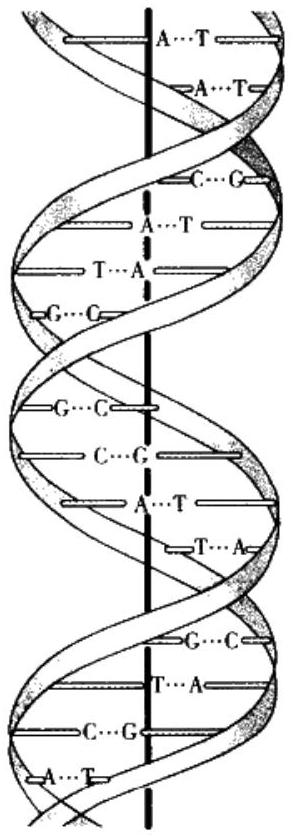
\includegraphics[max width=\textwidth, center]{2025_05_15_6a28331d5e7c993ad07ag-590}

图 13-1 一个互补的双螺旋的示意图。两个糖一磷酸盐的脊椎在外面卷曲着。平躺着的基组成核,它们成对出现——A 总是和 $\mathbf{T}$ 连接, $\mathbf{C}$ 总是和 $\mathbf{G}$ 连接。该结构形成一个螺旋楼梯,成对的基形成胗梯。\\
摘自于 J.D.Watson,The Double Helix.p.130,这里的引用得到版权所有人 G.S.斯坦特的同意。

5 和 6.演绎和检验结果。假说已经形成,接着要对它进行检验。首先,直接的推论是:如果华生和克瑞克提出的双螺旋确实是对 DNA 的正确解释,那么,构造这样一个三维的双螺旋模型是可能的,即所有基都被安排在内部,并且螺旋的角度以及链条的其他特点应当符合以前的 X 光图像及其他的实验结果。这个模型很快就得到了。

许多其他的理论推论被得到,每一个推论的检验都获得了成功。令分子生物学家长期困扰和沮丧的某些数据,由于这样的分析而得以理解。人们了解到,来自于父母的生殖细胞中的 DNA 数量,在普通细胞中只发现了一半。现在我们清楚了个中原因:如果双螺旋在生殖过程中裂开,来自于双亲的裂开的细胞自然只包含正常 DNA 数量的一半。华生一克瑞克对 DNA 结构的解决的正确性的证据迅速增加;不久,他们的假说非常充分

地得到证实。\\
7.应用。华生-克瑞克关于 DNA 结构 128 页的报告 ${ }^{[22]}$ 创造了科学史,它对生物学进程的改变是巨大的也是持久的。该知识的广泛且威力强大的运用将他们的成就推到顶峰。在随后的几十年里,人们认识了 DNA序列中使用的编码;整个人类基因组的完整图实际上是完全的,不久人类将得到该图。将 DNA 链进行切割、重组的技术已经得到发展,它们已经在新药、疫苗和人造荷尔蒙的制造中普遍地得到应用。重新组合 DNA 技术仅在 DNA 结构被最终解决的条件下才是可能的,该技术的应用使生物学和医学发生革命,并且仍保持着旺盛的应用生命力。

\section*{13.6 判决性实验和特设性假说}
\section*{A.判决性实验}
科学中的进步很少是直接的和容易的。认为通过对某个问题简单地使用几步假说一演绎法就能够达到答案,这种看法是愚奪的。答案一一正确的说明性假说一一往往是模糊的,需要非常精心制作的理论武器。建立最后的正确假说会极其困难。这个过程完全不是机械的,除了需要艰辛的观察和实验外,还需要深刻的洞察力和很大的创造性。

新的假说得以形成之后,如果它与某个先前已经接受的理论相矛盾,很难确定哪个正确。在某些场合下,两个竞争性假说用被称为一个"判决性实验"的东西进行检验。判决性实验是指这样一个实验,它被精心构造出来以表明所提出的说明中的一个而非另一个实际上是正确的。这样的判决性实验一旦被建立起来,可能是激动人心的和极其有成果的。

例如,美国物理学家阿尔伯特•迈克尔逊和化学家爱德华•莫雷在 1887年精心构造了一个测量光速的实验。通过这个实验使一个被广泛接受的理论(他们原来相信它是正确的)置于一个判决性实验之中。人们长期相信空间中充满着一个被称做"以太"(ether)的假设物质,(人们假定)该物质使光波运行,如同空气使声波运行一样。或者以太存在,或者它不存在。如果它存在,那么测量出的沿着地球运动方向的光速,应当与地球运动成一个直角方向上的光速不同。该实验产生了一个"否定的"结果。因该实验是一个对当时被广泛接受的理论的判决性检验,它成为物理

学史上最著名的实验之一。没有发现这两个不同方向上运动的光速存在差别。这个结果有力地破除了人们长期相信的以太概念。 ${ }^{[23]}$

但是遗憾的是,威力如此强大的判决实验不总是可行的。不同的可观察结果可能不会从不同假说中推演出来;或者,它们能够被推演出来,但是我们没有能力创造条件,以检验哪一个假说的结果将出现。

物理学在 21 世纪初面临的一个主要问题也正属此类。在两个最强有力的理论之间,存在一个明显的目前不能解决的冲突。广义相对论已经得到很好的证实,其定律(描述引力以及引力如何形成空间和时间)的一个必然推论是:某些塌陷的大质量的恒星将形成"黑洞",从该黑洞中逃脱是不可能的,因为它要求比光要快的速度。量子力学定律同样得到很好证实,但它们明确推论得,信息不能永久消失,即使掉到黑洞里也是如此。要么存在某个目前还不知道的时空性质,它能够用来对该信息的保持进行说明,要么在物理学中存在错误,指出它可以对该信息的永久消失给出解释。最终两个理论中的一个必定得到修正,但我们现在仍然不知道哪个要修正,我们也无法构造所需要的判决性实验。 ${ }^{[24]}$

判决性实验是科学探究一个重要方面,然而与构造判决性实验相关的另外一个困难是,人们提出某个说明性假说,我们希望通过进行某个判决性实验来检验它的推论,但它的推论不可能仅从该假说自身演绎出来。我们是使用该假说与其他理论一起而推论得到要检验的结论的。为此,我们假定那些其他理论完全可靠。它们确实可能是完全可靠的,当然它们也可能不完全可靠。如果它们不可靠,即使判决性实验似乎否证了待考察的假说,也有可能待考察的假说恰恰是正确的。科学中的进展依赖于假说集合,其中的任何一个都可能是有缺陷的。

当涉及相当高抽象程度的假说时,仅仅单个假说不可能直接演绎出可直接检验的预测。用做演绎前提的必定是一个统一的假说群体,如果观察到的事实不是预测的事实,那么我们可以得出结论,该假说群中至少一个是错的。但是,这个结论不能表明哪一个假说是错的。例如,在前面的对 DNA 结构发现的解释中,华生和克瑞克在检验核酸丝的形式是双螺旋、它的基指向内部的假说时,他们发现这样的安排不能与所有已知的事实和已接受的理论相一致。"已知的事实和已接受的理论"——水含量、双螺旋斜度、基(腺嘌呤、鸟嘌呤、氧氨嘧啶和胸腺嘧啶)的连接方式——在假说的检验中被假定是正确的。如果所有这些假定的确正确,长丝的结构

不可能是双螺旋。然而,在实际中,华生和克瑞克对他们的假说有足够的自信,他们开始怀疑描述基(A、G、C 和 T )相互结合的理论不完全正确。该理论被他们放弃,他们提出一个不同的理论,即假定结合物是氢的理论,此时,双螺旋的新假说(以及与之相连的理论)得到证实。

因此,在揭示一群假说有缺陷的过程中,一个实验能够是"判决的"。这样一群假说通常包含许多独立的假说。其中任何一个假说,无论实验结果对它多么不利,我们可以拒绝该群体中的某个其他假说,而坚持它的真理性。这就使得某些人得出结论说,从来不会有单个假说遭受判决性的实验。

\section*{B.特设性假说}
针对上面的批评,有人认为,一个实验在否证单个新假说中的确能够是判决性的,因为通过拒绝假说群体中某个其他假说(上面已经表明这是可能的)而"拯救"该假说的努力是完全特设的(Ad Hoc)。Ad Hoc 为拉丁术语,字面意义是"为此[特定目的]"。Ad Hoc 包含这样一个意思,所有的假说都是特设的。因为,一个假说之发明如果不是为了解释某个先前得到确立的事实或者其他事实,那是没有意义的。但是当我们以这样的意义滥用它的时候,特设性意味着,对假说集合进行调整仅仅是为了拯救被检验的假说这样一个目的,它没有其他的说明力或者可检验的结果。

没有科学假说是这第二个意义上特设的。如果"鬼是机器故障的原因"被用来解释一个复杂的机器发生故障,那么它明显不是科学的解释;我们嘲笑这样的假说,它是否定意义上特设性的。但是,在任何实际科学研究中,当一个新的假说之提出以调整一个旧的理论的时候,该调整是否是该否定意义上特设性的,这需要进一步确定。

科学史中的另外一个例子可以帮助我们弄清这个问题。在19世纪,天体力学理论被人们很好地理解。对于天文学家来说,天王星和水星这两个行星的轨道与当时所接受的理论对它们所预测的轨道不一致。行星运动的理论在当时应当被修改,但是事实上它被保留了下来。为了解决该理论的协调问题,有人提出,存在某个未发现的行星,其引力造成观察到的反常现象。引起天王星轨道偏差的新行星的轨道,由勒维烈在 1845 年预测出来,预测结果不久被海王星的发现而证实,其位置精确地解释了那些偏 513 差。 ${ }^{[25]}$ 这个假说——存在这样一颗行星——当然不是否定意义上特设性的假说。原因是,从该假说中能够演绎出许多结论,该假说是独立可检

验的。\\
但是在水星的案例中,存在另外一颗行星[该行星过早地被命名为 "火神星"(Vulcan)]干扰水星轨道的假说,不能得到证实。如果一个理论假想有"水星力",用它们来解释水星轨道的异常,而这些力不能解释其他任何事情,并且绝不能被找到,那么这样的一个理论发明自然是特设性的。实际情况是,该疑难长期得不到解决;直到1915年广义相对论提出后,观察到的水星轨道的不规则,才完全与不同的但完美的天文学理论相吻合。水星轨道异常,能够使用广义相对论来预测,这个事实构成该理论最引人注目的证实之一。爱因斯坦称它为"我生命中最辉煌的工作"${ }^{[26]}$ 。只有在那个时候,我们才给出了关于该现象的合适的(即真正理论化的)说明。

天文学史中的这个疑难给出了人们在使用特设性这个术语的第三个意义,它也是否定性的:表示一个单纯的描述性概括。一个描述,它是第三个意义上特设性的,它仅断定一个特定种类的所有事实只在某些特定种类的条件下发生;但是该假说和前面的那些特设假说一样没有任何解释力或解释范围。这样的假说的一个古典例子是,"菲兹吉拉德收缩效应"被提出来对迈克尔逊-莫雷在光速实验结果的解释。菲兹吉拉德断定,物体以极其高的速度运动会发生收缩,他确实对给定现象给出解释,并且他的假说能够为重复进行的同样实验所检验。但是他的"收缩效应"不能解释其他的任何东西。在当时它被普遍认为是特设性的而不是说明性的。(正如与水星行为中出现明显差别的情况一样)直到相对论的提出(爱因斯坦的狭义相对论),人们才得到迈克尔逊一莫雷实验结果的一个合适的理论说明。

我们可这样总结,实验对单个假说绝不能是判决性的,这不仅因为假说经常是在否定意义上特设性的;进一步地说,在本节前面已经表明,因为假说只是在群体中才是可检验的,实验绝不能成为判决单个假说的东西。 ${ }^{[27]}$ 这个限度阐明了科学的系统化特点。科学进步就是建立永远更加恰当(ever-more-adequate)的理论,以便解释不断增加的观察结果和实验事实。某些分离事实能够具有较大的价值,因为科学的最终基础是事实。但是科学结构主要不是通过点滴累积而得以发展的,其发展是在一个已得到普遍认同的理论体系的框架内整体地进行的。认为科学假说或者定律是分散的和独立的观点是朴素的,也是过时的。

在这样一个理论框架中工作,此时我们不对该理论框架进行质疑;进行一个"判决性实验"以证实或否证某个假说的观点仍然能够有意义。如果得到一个否定性结果,即,根据某个有疑问的假说与已经接受的科学理论一道进行预测的某个现象,它没有发生,那么该实验是判决性的,这个有疑问的假说可以被拒绝。但是正如我们已经看到的,在这个过程中不存在任何绝对的事情,因为,那些即使被人们普遍接纳的科学理论面临新的和矛盾的证据时,也要发生调整。科学无论在实践中还是在目标上,都不是一成不变的。

从前面的讨论中得到的启示是,将"隐藏的假设"揭示出来,以便能够对那些默认的假定进行重新审视,这在科学进步中是重要的。当一个关键假设是潜藏的时候,没有明显的必要,因而没有好的机会对之进行考察并确定它到底是真还是假;通过将以前潜藏的假设揭示出来,对之进行分析并(也许)否定它,科学往往获得进步。

例如,在日常生活中谈论两个事件"在同一个时刻"发生,这似乎完全没有问题。我们普遍假定事件常常同时发生。但是科学中一个重要的和巨大的进步开始于爱肉斯坦将这个假定揭露出来。他问,一个观察者如何能够确定两个距离遥远的事件是否真的在同一时刻发生。最终他得出这个结论:两个事件对于某些观察者来说能够是同时的,但对其他的观察者来说则不是;这依赖于观察者相对于待研究事件的相对位置和速度。正是对同时性假定的拒绝,使爱因斯坦发明了狭义相对论,从而为解释迈克尔逊——莫雷实验所揭示的现象跨出了重大的一步。当然,一个假定在它被挑战之前必须被人们所认识,因而,在科学中具有重大意义的是,将理论中起作用的所有有关的假定揭示出来,而不让任何一个隐藏起来。

通过描述和讨论科学史中最辉煌的篇章之一一伽利略对太阳系的哥白尼理论进行的观察证实,是对科学方法的进行总结并阐释科学整体的进步的意义的极好的途径。

到 16 世纪早期,人们对行星相对于恒星的运动进行了仔细研究,已能够预测行星的显著运动。同样被大量研究的月亮,在神学家看来是一个完美的球。天上的物体被认为在形状和运动上都是无缺陷的,它们围绕地球以完美的圆周来运行。地球是由上帝创造的世界的中心。1609年伽利略发明了 20 倍的望远镜,它的主要用途,起初人们能够想到的是在航海

方面,或者用做军事方面。1610年1月,伽利略用这个工具偶然地观察了天空。在该月 7 日他写了一封长信,详细汇报了他对月球和其他天体所做的观察。他写道:

我用我的一台望远镜观察了……月亮的表面,对之我能够看得十分贴近……能够非常清晰地看清那里存在什么;事实上看到的是,很明显月亮的表面一点不均匀、光滑和规则,与许多人对之以及其他天体所认为的不一样。相反,它粗㯧和不均衡。简言之,健全的推理只能得出,它(月亮)充满与分布于地球表面的山峰与山谷类似的突出物和洞穴,但大得多……[28]

为了拯救月球确实是一个完美的球的假说,从而维护天体的神学解释的融贯性(月球的完美是其中的一个部分),一些伽利略的批评者后来蛮横地提出了特设性的假说:月球表面的明显洞穴和不规则事实上充满着一种无㻓疵的水晶般的神圣物质,因而通过伽利略的望远镜是观察不到的。

伽利略不仅考察了月球,他在信中进一步写道:

除了月球的观察之外……用望远镜可以看到其他恒星,(否则)是不清晰的;仅仅今天晚上,我看到了木星由三个恒星所伴随,用肉眼它们完全不可见,并且其形状是这样的 ${ }^{[29]}$ :

在该处,伽利略插了一个略图,见图 13-2。图中,三个恒星在一条直线上,两个在木星的东面,一个在木星的西面。他观察到,它们的距离不超过 1 个经度,但至少那个时候,他认为它们是恒星,它们离木星的距离以及它们之间的距离是相当粗糙地得以表示的。

第二天,1610年1月8日,伽利略碰巧再次观察木星;那些"恒星"的较早的位置幸运地被他勾画在那里。他的信没有发出;在信纸的底下, 517他写道:

在第8日:[他釈入了一个草图,该草图描绘了木星和三颗星,它们相互之间比较靠近并且几乎等距离,并且三颗星均在木星的西面!]\\
在1月7日看到的木星是:

\begin{center}
\begin{tabular}{|l|l|l|}
\hline
东* & \begin{tabular}{l}
10. \\
そ*** \\
\end{tabular} & \begin{tabular}{l}
11. \\
*** \\
\end{tabular} \\
\hline
\end{tabular}
\end{center}

在8日\\
子罒***木星由西向东运行,而不是倒行的\\
在12日看到的是这样的位置:东***西\\
在13日看到的是,4颗星十分接近木星: ****更精确的为:\\
在14日看云\\
在15日\\
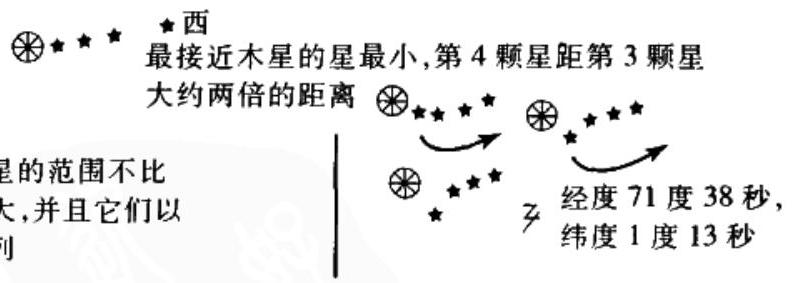
\includegraphics[max width=\textwidth, center]{2025_05_15_6a28331d5e7c993ad07ag-597}

图 13-2 伽利略信中的一幅图。伽利略于1610年1月7日开始写这封信,这封信记录了他首次对木星的 4 个卫星的不朽观察,因而证实了哥白尼天体运行理论。他打算将这封信寄给威尼斯总督,并打算将一台望远镜送给他。伽利略偶然地保存了该信,在该信纸的底部,他对他的观察做了重要说明。图中下面部分即为翻译后的内容。(得到密歇根大学典藏图书馆的允许。)

这给伽利略带来了一个严重的理论问题,因为当时这些新发现的星星是恒星的假定没有被怀疑。因而,它们出现在木星的另外一侧需要用木星的运动来解释。在 8 日,他加了一个说明:

因而它[木星的运动]是由西向东运行的而不是倒行的。

如果第8日木星在所有三颗星的东侧,而之前的一天木星在它们中的两个的东侧,木星必定已经移动,必定以可靠的天文学计算相反的方式运动!人们可以想象伽利略等待次日观察时的兴奋;他直接的观察与他的计算会如此截然的不一致吗?但是第9日天空中有太多的云而无法观察。在第10日,木星显然已经移动回西侧去了,而使第三颗星变得模糊,另外两颗星再次在该行星的东侧!在1月11日,一个类似模式被观察到,而在该夜里伽利略后来写道:

与木星相对靠近的星是另外一颗星的一半大小,并且十分靠近它,而其他的晩上这三颗星看起来同等大小、相隔也相等……

明显的,必然要得出某个事情。从已接受的理论和信念,能够自信地得出关于木星的一个演绎的预测:如果三个新星是恒星,并且伽利略的观察是精确的,那么恒星的运动是不会发生的。人们可以通过修补整个天文学计算,而拯救那些新星是恒星的信念,但是这些没有受到严重的怀疑;或者,人们能够对伽利略的观察的精确性提出挑战,这也是他的一些批评者后来努力做的,他们称伽利略的望远镜为魔鬼的工具。伽利略对他所看到的毫不怀疑,并且他迅速抓住已接受的假说集合中的必须放弃的成分,这使他的刚愎自用的对手很沮丧。他对他在 11 日继续进行的观察进行说明:\\
……从望远镜中,似乎是,存在三个环绕木星运动的恒星,此时其他人是无法看见它们的。

他后来写道,这三颗运动的恒星:

以后的几个晚上的观察证实了他的革命性结论。该结论与他对月亮的早期观察一起,对被广泛地并教条地接受了几个世纪的天体理论产生了严重质疑。

1610年1月13日,伽利略观察了第四颗"星",因此木星的第四颗卫星被发现。这些观察为哥白尼假说提供了强有力的证实。哥白尼的天体理论很难与伽利略时代建立完好的神学教义相协调。木星的这些卫星(自从那时更多的卫星被发现)木卫一、木卫二、木卫三、木卫四被合适地称为 "伽利略卫星"。在晴朗的夜晚当木星可见的时候,任何人都可用一个普通的双眼望远镜容易重新确证这些革命性发现。

\section*{13.7 作为假说的分类}
存在这样一个观点,假说仅在比较发达的科学中而不是在相对不发达的科学中才发挥重要作用。这个观点应当被拒绝。有人主张,尽管说明性假说在物理学、化学这样的科学中起重要作用,它们在生物学和社会科学中则没有这样的作用,或者至少现在没有这样的作用;后者仍然处于描述性阶段,而假说方法对所谓描述性的科学如植物学、历史学是不合适的。我们很容易对这个观点给出反驳。对描述本性的考察将显示,描述本身是建立在假说之上的,或者说描述本身包含假说。假说在生物学的不同体系的分类法或分类学中是基本的,在历史学或其他社会科学中假说也是基本的。

在历史科学中,假说的重要性容易得到阐明,我们首先讨论它。一些历史学家相信,历史研究能够揭示存在着的单个宇宙目的或模式,该目的或模式或者是宗教的或者是自然的,它对有记载的历史的整个进程进行解释或说明。其他的历史学家则否认有任何这样的宇宙设计的存在,但他们坚持认为,历史研究将揭示某个历史规律,该规律解释过去事件的实际次序,并能够用来预测未来。无论哪种观点的历史学家,他们寻求的说明必须解释过去记载的事件,并被它们所证实。因而,无论是哪种观点,历史学是一个理论性的科学而不仅仅是描述性的科学,必须承认假说在历史学家事业中的中心作用。

然而,有第三种历史学家,他们更为谦虚地设定他们的目标。根据他

们的观点,历史学家的任务只是简单地将过去进行编年史记录,即以他们的编年史顺序将过去的事件进行简单的记录。似乎是,根据这种观点, "科学的"历史学家没有进行假说的必要,因为他们所关心的只是事实本身,而非与事实有关的理论。

但是过去的事件没有像该观点试图使我们相信的那样容易编年。过去本身不能提供这种记录。现在能够得到的是现在的记录和过去的痕迹。它们的范围是:从关于过去的官方档案,到对半传说式的英雄的征服行为的赞美的史诗;从以前的历史学家的作品,到考古学家挖掘出土的过去年代的物品。这些只是历史学家能够获得的事实,而从这些事实中他们必须推论得出过去事件的本质——这是他们描述的目的。不是所有的假说是全称的,有些是特称的。历史学家关于过去的描述是特称假说,使用该假说的意图是解释现有数据,而现有数据构成了它的证据。

从大范围来看,历史学家犹如侦探。 ${ }^{[30]}$ 他们的方法是共同的,遇到的困难也类似。其困难主要是证据不充足,并且,许多证据如果不是被笨手笨脚的地方警察所损坏,就是被相关的战争和自然灾害所破坏。正如罪犯可能留下了假的或误导的线索以甩掉追踪者,太多的现存"记录",据说是对过去的描述,而实际上是对过去的歪曲:或者是有意的,如"康斯坦丁的赠款"这样伪造的历史文档的案子,或者是无意的,如早期没有批判性的历史学家的著作。正如侦探建立和检验假说必须使用科学方法一样,历史学家也必须如此。即使将自己限于对过去的纯粹描述的那些历史学家,也必须使用假说来工作:他们是理论家,不管他们自己是如何认为的。

生物学家所处的位置稍微有利。他们处理的事实是现在的,易于检查。为了描述一个地区的动植物群落,他们不必精心构造历史学家那种遭到诟病的复杂推理。数据可以被直接地认识到。对这些项目的描述不是因果的,而只是系统的。他们被认为是对动物和植物进行分类,而不仅仅描述它们。但是分类和描述实际上是同一个过程。将一给定动物描述成食肉类,即是将它分类为一个食肉动物;将它归类为爬行类,即是将它描述成爬行动物。某个物体被描述具有一个给定属性,即是将之归类于具有该属性的对象类中的一个成员。

分类,正如通常理解的那样,不仅仅要将对象划分成不同的群体,而且要将每个群体进一步划分成次一级的群体或次一级的类,等等。这个模

式是我们大多数人所熟悉的:如果不是从学校学习中知道,那么可能是从 "动物,植物,还是矿物?"这个古老的游戏(或者更普遍地被叫做" 20个问题"${ }^{(1)}$ )中获得。分类是一个普遍的需要。原始人不得不将草根、浆果划分为可食用的还是有毒的,将动物分为危险的还是安全的,以及将部落分为友善的还是敌对的。所有人都根据自己的实际需要而进行区分,并忽视那些在他们的事务中不怎么重要的区别。农民会对谷物和蔬莱进行小心和仔细的分类,而将各种花只统称为"花";而卖花人却会细致地将他们的商品进行分类,而将农民的所有收成一起称为"农产品"。

我们对事物进行分类有两个基本的动机。一个是实践的,一个是理论的。某人仅有 3 或 4 本书,他对它们了如指掌,他一瞥就能够分辨它们,就此没有对它们进行分类的必要。但是在一个包含上万册书的图书馆里,情况便不同。如果不对图书进行分类,图书管理员就不能找到所需要的书,该图书馆的收藏将无实际用处。物体数量越大,越有必要对它们进行分类。分类的实际目的是使大量的采集成为可能。在图书馆、展览馆和各类公共记录展厅的情形中这特别明显。

当我们考虑分类的理论用途时,我们必须认识到,使用一种分类法或另一种分类法与真理和错误无关。可以用不同方式、以不同的观点来描述物体。使用的分类方案依赖于分类者的目的和兴趣。例如,图书管理员、图书装订商和藏书家对书的分类便有所不同。图书管理员根据书的内容或主题对书进行分类,图书装订商根据的是装订方式,图书收藏者根据的是印刷日期和相对稀有程度。当然我们不能穷尽各种可能性:图书包装者会根据书的形状和大小对书进行分类,而对书有其他兴趣的人根据他们不同的兴趣进行不同的分类。

那么,科学家的什么样的特别兴趣或目的,使他们偏爱一个分类方案而不是另外一个?科学家的目的是获得知识:不仅仅是关于这个或那个特别的事实的知识,尤其是关于用事实来确认的普遍定律的知识,以及事实之间因果连接的知识。从科学家的观点来看,一个分类方案比另外一个要好,一定程度上在于,在得出科学定律的过程中它是更富于成果的,并且在形成说明性假说过程中它是更有帮助的。

\footnotetext{(1)这是一个游戏。多人确定出一个东西,让另外的人通过询问问题来猜他们所确定的是什么东西。
}对物体进行分类,其理论的或科学的动机是增进这些物体知识的愿望。事物的知识的增加可以增进我们对事物的属性,它们的相似性及差别,以及它们的相互关系的进一步理解。一个分类方案如果只为狭窄的实际目的而制定,就可能抹杀了重要的相似性和差异性。把动物划分成"危险的"和"没有危险的",如把野猪和响尾蛇归为一类,把家猪和草蛇归为一类,这种划分为了强调表面的相似性,而忽视了更本质的相似性。对物体的任何科学的、富有成果的分类需要具有关于它们的大量的知识。对比较明显的特征的粗浅了解,会使人们将蝙蝠作为会飞的生物归为鸟类,把鲸作为生活在大海中的生物归为鱼类。如果我们具有更广阔的知识,我们便将蝙蝠和鲸两者均归为哺乳动物,因为它们都属于温血、胎生并哺育幼崽的动物——这些是分类所根据的更为重要的特征。

如果一个特征能够作为线索,以发现其他特征,它便是重要的特征。从科学的视角来看,一个重要的特征是指这样一个特征:它与许多其他的特征有因果连接关系,因而它能够作为最大数量的因果律的框架,并且有助于形成最普遍的说明性假说。因此,这样的分类方案是最好的,如果它建立在所要分类的物体的最重要的特征之上的话。但是正如我们已经强调的那样,我们事先并不知道会得到哪些因果律,而且因果律本身也带有假设的性质,因而,在哪个分类方案是最好的问题上的决策本身就构成一个假说,一个后续研究可能将之否定的假说。如果后来的研究揭示了,其他特征更为重要(即它与大量的因果律和说明性假说相关),我们能够合理地预期,原来的分类方案应当被否决,我们会选取基于更重要的特征之上的新的分类方案。

分类方式是假说的观点被它在科学中实际所起的作用所证实。分类学是生物学中一个正统的、重要的并且欣欣向荣的分支学科。在生物学中,某些分类方式.如林奈的分类法,被采纳、使用,后来因有了更好的方案而被弃用;更好的方案本身在新的数据下也经受着修改。一般来说,在科学的早期阶段或不发达阶段,分类最为重要。然而,随着科学的发展其重要性不一定总是降低。例如,由门捷列夫表所表明的元素的标准分类法、仍然是化学家的一个重要工具。

前面对自然科学中使用分类的解释,可启发我们进一步认识在历史研究中使用分类的重要性。我们已经说明,历史学家对过去事件的描述本身即是基于冒前资料之上的假说。然而,假说在描述的历史学家的事业中发

挥着另外一个同等重要的作用。任何数量级的历史事件都不能被完完全全地描述。即使人们能够知道它的所有细节,历史学家也不可能将之全部写进著作之中。生命过于短暂,它不允许人们对事物进行详尽无遗的描述。因此,历史学家必须对过去进行有选择地记载,记录下的仅仅是过去的一些特征。历史学家进行选择的基础是什么?显然,历史学家要叙述的是有意义的或重要的,而忽略无意义的或琐碎的。这个或那个历史学家的主观偏见会使他或她过分强调历史进程中宗教、经济、人物或其他某个方面的作用。但如果历史学家们考虑到,要做出客观的或科学的评价,他们便会重视那些能够形成因果律和普遍的说明性假说的因素。自然,这样的评价会随着进一步研究而经受着改变。

西方第一个历史学家希罗多德(Herodotus)细致描写了他编入编年史的事件,有人物的、文化的,以及政治的、军事的。所谓第一位科学的历史学家修昔底德,将自己的写作更多地限于政治和军事方面。在很长一段时间里,大多数历史学家跟随修昔底德,但是现在钟摆正摆向另外一个方向:历史学家十分重视过去的经济和文化方面。正如生物学家的分类方案包含了他们的假说——通过这个假说生物的特征与最大数量的因果律相关联,历史学家选择用一个典型事件集合而非另外一个集合来描述过去事件,这种选择包含了他们的假说:什么样的典型事件与最大数量的其他典型事件因果地连接在一起。这样的假说是必需的,哪怕历史学家对过去进行系统的描述的工作只是刚刚开始。正是分类和描述——无论是生物学的还是历史学的一一所具有的假说性的特点,使我们将假说看成是科学探究的通用方法(the all-method)。

\section*{练习题}
在下面的段落中:(a)解释了什么现象?(b)提出了什么假说来解释?(c)请用13.3节提出的标准评价这些假说。\\
-1.在对"新世界"(new worlds)的令人眼花缭乱的探索中,两个加利福尼亚天文学家,乔弗里•玛茜博士和保罗•布特勒博士今天报告说,探测到两个围绕如太阳般的恒星运行的行星。行星的温度似乎足够温暖,水能够以液态的形式存在,这是一个产生地球外生命的化学过程的发生条件。

这两个最新发现的太阳系外行星,环绕室女星座中 70 号星和大熊星

座中的 47 号星。它们的距离是 35 光年,从宇宙的尺度来说相对较近。它们太小,也太暗,在它们环绕的恒星光芒的照耀下难以被看到,但是它们的重力场已经确定无疑地被建立起来。

天文学家说,两个星系类似于太阳系,大小、温度和年龄上均差别不大。迄今,人们对其他行星的寻找集中在离地球 100 光年之内的大约 120个与太阳类似的恒星上。

布特勒博士观察到,室女星座中 70 号星的运动中所发生的摆动,精确按照一个大行星的轨道运行,他说:"我对我们刚刚观察的东西十分肯定。毫不夸张地说,我几乎情不自禁地从椅子上站了起来。"

就科学家所知,其他的比较小的行星也环绕这些恒星。但是现有的技术无法探测到它们。在采访中,玛茜博士说:

\begin{displayquote}
现在它们给理论工作者造成了巨大挑战。它们比太阳系有更多的东西需要解释。其他的星系可能具有更多的变化,可能包含难以进行常规分类的物体。
\end{displayquote}

-_"Hints of Life in Space",New York Times, 18 January 1996

2.基因如何影响寿命?精细蚵虫 C.elegans 正常只活 3 周。但是如果它的某个基因发生了突变,它的寿命将能够是正常寿命的四倍。蚛虫身上有长寿基因吗?如果确实有、并且能够找到的话,那将为人如何活得更长提供线索。1999 年发现的一个蛔虫基因表明,影响冬眠期的突变和影响人类寿命的突变(如由压力引起的)之间可能存在关联。新的基因被它的 (哥伦比亚大学)发现者们称为一个长寿基因(catalese),因为,当它被破坏后,其他的基因便不能够以预期的方法来延长寿命。

但是进化生物学家有理由怀疑任何长寿基因的存在。一个理由是,通常说来,自然选择不增加繁殖年龄之后阶段的适应性,因为活得较长的生物体不会产生额外的后代。此外,这些怀疑者认为,长寿基因会使繁殖期过后的动物大量涌现,它们会与它们自己的后代争夺食物。

\section*{--Reported in Nature, 13 May 1999}
3.一群人,他们买同样的东西,从同样的资源处进行娱乐,表现出类似的投票模式,并且其行为方式相当类似。这是人的分群现象(popu-\\
lation clusters)。迈克尔•J•魏斯区别了 62 种分群,他称它们为"有特色的生活类型"。他给它们取了名字并阐明了它们的独特特点。

例如,在"城镇礼服派"(Towns and Gowns)那里,龙舌兰酒比其他地方要更为普遍,观看肥皂剧《另外的世界》的观众比其他地方的多一倍。在"军事派"(Military Quarters)中,人们观看电视剧《硬拷贝》的可能性是平均美国人的四倍。在那些住在郊区的年轻的中产阶级美国人中,对家具表面进行整修、高山滑雪、养猫反常地普遍,而下棋、打扑克则反常地不普遍。

人们发现,对商家寻找顾客、对候选人拉票、对非营利组织招募新的志愿者,等等,生活类型分群都是有用的。看上去琐碎的事情可能有相当的启迪作用。在华盛顿,魏斯观察到"布里白奶酪的爱好者——他们停下正在进行的工作而武断地表达意见,那些克拉夫特•威尔塔奶酪爱好者——他们维系着服务经济,在他们之间存在一种不良关联"。他询问:"什么东西使我们中的一部分人吃布里白奶酪,而其他人狂吃威尔塔奶酪?"\\
-Michael J.Weiss,The Clustered World (Little,Brown,2000)\\
4.在所有社会科学中最有挑战性的问题之一是,弄清家庭环境和家族基因对孩子智力、职业和经济成就的影响。父母的教育水平与他们的子女在学校的成绩和智力测试分数,表现出极高的关联。人们通常认为,这种关联显示的是环境对求学成功的影响强度。因为,求学时间较长的父母期望他们的子女取得好成绩,与受较差教育的父母相比,他们会为子女创造更好的教育环境。如果富裕家庭环境与孩子的学习成绩之间存在因果关系,那么,这是有意义的:引导所有父母提供更好的教育环境,作为改进成绩差的学生的一个方法。

然而,如果智力在一定程度上是遗传的,那么因果连接会不同:具有高智力水平的父母将比其他人求学的时间更长,他们会把他们的部分智力遗传给他们的子女,并且会创造更好的家庭教育环境。根据这种观点,家庭环境和小孩学校表现之间的关联,可能掩盖了一个在父母的智力和其子女智力之间的更加重要的关联。\\
-Harry L.Miller,"Hard Realities and Soft Social Science",The Public Interest,\\
*5.人们经常研究在趋地性(geotropism)中的刺激反应机制。如果将刚露出根和茎的幼小树苗以任何的位置固定,幼小的根将固定不变地向下生长,而茎向上生长。英国园艺家奈特在一个世纪以前认为,该行为应归于重力。他推理说,如果这是对的,那么,应当可能的是,用一个更强的力来代替重力将改变生长方向。奈特将多个幼小的植物绑在轮子的边缘四周,他在水平方向上迅速转动轮子,从而使植物经受比重力大的离心力。在这些条件下,植物的根在离心力的拉动下向外生长;而茎向内生长,朝向轮子的中心,其方向与根的方向完全相反。于是奈特证明了,植物的结构针对这种离心力确定生长方向的方式,与它们针对重力确定生长方向的方式是完全一样的。\\
----Edmund W.Sinnot and Katherine S.Wilson, Botany:Principles and Problems\\
6.一个研究小组近来对在健康护理研究会注册的 79109 名妇女进行研究,试图寻找倒班和心脏病之间的关系。1988 年,研究人员询问这些妇女,她们倒夜班的年数。当时,她们中没有人有冠心病病史。许多妇女经历了倒班,其中 $7 \%$ 的妇女倒班年数达 15 年或更长。与那些从没有倒班工作过的妇女相比,倒班工作的妇女体重更重,并更有可能吸烟。较长时间的倒班往往造成高血压和糖尿病。在随后的四年时间里, 292 名妇女有冠心病的迹象。倒班的妇女发展成心脏病的可能性要高 $40 \%$ ,倒班年数越长,得综合征的可能性就越高。倒班超过 6 年的妇女患心脏病的危险增加了 $51 \%$ ,在随后的四年里死亡的可能性增加了 $29 \%$ 。即使研究人员排除了体重、吸烟以及许多他们能够找到的其他引起心脏疾病的因素,倒班的影响仍然存在。

但是,倒班本身就是元凶吗?还是倒班的妇女与不倒班的妇女,在该研究没有探测到的或者没有考虑到的方面存在不同?这些问题不通过这样的实验是解决不了的:在实验中,大量的妇女被随机地、长时间地安排进行倒班工作或正常作息时间工作。该实验也不可能在短期内完成。\\
-I.Kawachi,et al.,"Prospective Study of Shift Work and Risk of Coronary Heart Disease in Women",Circulation, 1 De- cember 1995

7. 10 个制药公司和伦敦的惠康信托公司在1999年4月宣布,他们将

努力绘制人类基因组的精密图。他们的目的是尽快揭示导致疾病的基因变化,从而发现新药物。

该联盟的特定的目标是,在两年的时间里,识别和确定人类 DNA 分子集合上的 30 万个"图点"(map points)。DNA 单位是已知的,每 1 万个核苷中大约有 1 个图点。图点是核苷的位置,在这些位置上,至少 $1 \%$的人具有的核苷与标准序列的不同。一个字母的这种差别被称为"单核苷多态现象"或简称 SNPs(读做"斯尼普丝")。在人类身上实际工作的基因占整个基因组大约 $3 \%$ ,因此大多数 SNPs 将处于不工作的区域里。但是,由于 SNPs 易于被识别,它们是将一个区域与另外一个区域区别开来的理想标志。接近一个特定基因的 SNPs 集合更可能随同该基因一同遗传,因而能够用 SNPs 来识别该基因。因此,基因学专家希望通过观察一个家族,如糖尿病流行的家族,而能够识别出与该病可能有关的许多基因,他们的目标在 SNP 联盟的帮助下,通过识别出现在糖尿病病人身上而不出现在正常人身上的 SNPs 的类型,而得以实现。

尽管该联盟的成员是获利公司,SNP 则不是一个营利的事业。它绘制的基因组图将是公开的。帕菲泽公司的研究主任,同时也是该联盟的成员之一的迈克尔•西尔伯博士说:"这种工具让所有的医学研究人员参与到发现之中,它应当是对公众开放的。"\\
-Reported in New York Times, 15 April 1999\\
8.最近科学家开始了他们迄今最雄心勃勃的努力:寻找和利用已被预测到但最难以捉摸的自然现象之一一引力波。早在1915年,阿尔伯特•爱因斯坦用他的广义相对论预测:宇宙中恒星生成和消亡这样的急剧事件将发出引力波,它使地球充满独特种类的辐射。但是科学家用越来越先进的探测器寻找了几十年,至今毫无所获。一个被称做激光干涉仪引力波天文台的设备被设计出来,它使引力波的探寻推向顶峰。

引力波的发现会被看成是现代物理学和天文学中最辉煌的发现壮举,它能够给爱因斯坦的广义相对论提供新的确证。爱因斯坦的广义相对论是现代科学的基础,而它的有效性难以用实验来证明。该理论使人们不再认为空间是虚无的,而认为空间是由空间和时间的一个弯曲结构组成。根据该理论,当恒星发生塌陷的时候,时空结构中的波纹会以光速向各个方向发出;这些波纹并不传递引力,但是它们使引力发生扭曲。

理论上讲,来自于遥远宇宙事件中的引力波对地球上的物体造成的移

动,应当是微乎其微的,移动的距离比原子核的距离要小得多。新的天文台被设计得足够敏感,以测量这些波,并查明它们来自于宇宙何处。在持怀疑态度的人看来,存在的风险是该设备将不够敏感,探测不到引力波。\\
----"Ambitious Effort Aims to Find Gravity Waves",New York Times, 27 February 1990\\
9.春季出生的男性比秋天出生的男性要高些。维也纳大学的研究人员在10年间,对507125 个奥地利男性的出生时间和身高进行分析后,得出结论:春季月份里出生的男性平均比在秋季月份出生的男性平均高约四分之一英寸( 0.6 厘米)。这些科学家由该大学人类生物学研究所的杰哈德•W•韦伯所领导。他们说,他们不能给"为什么身高与出生月份呈现这样一个明显的周期以一个明确的说明"。但是他们注意到,这种规则性可能与产生荷尔蒙褪黑激素的松果腺的光线依赖性有关,光线依赖性影响到生长荷尔蒙的产生。\\
-Reported in Nature, 9 February 1998\\
*10.若金星自转如此缓慢,我们可能试图得出结论:金星与水星一样,总是一面朝向太阳。如果这个假说是正确的,我们应当得出,黑暗的一面会出奇冷。配第特和尼科尔逊测量了金星黑暗的一面的温度。他们发现,该处的温度并不低,温度值为华氏 -9 度,比明朗的白天里地球大气层外要暖和得多。金星明亮的一面的气流不可能对黑暗的一面永久地进行加热。该行星自转必定相当快,以使黑暗面免于极度地冷。\\
-Fred L.Whipple,Earth,Moon and Planets\\
11.一年中特定季节里的太阳光的照射量产生了大量意想不到的结果。它可能增加春季月份出生的人的身高(在练习9中已经做了说明)。它同样可能增加遥远北方的居民夏季自杀的可能性。宾夕法尼亚州立大学医学院的心理学家保罗•科特尔写道,在阿拉斯加,出生于夏季月份的本地居民自杀人数占自杀总数的百分比为 $33 \%$ 强,与此形成对比的是,其他三个季节中每一个季节出生的人自杀百分比为 $22 \%$ 。他推测道,除了出生的季节不同造成了荷尔蒙不同外,由于在夏季里许多父母工作的时间十分长,夏天出生的婴儿可能与他们的父母接触机会比冬天出生的婴儿要少,在冬天,父母有更多的时间与他们的婴儿待在一起。\\
-American Indian and Alaska Native

12.人们想知道一个社会学谜的解,但人们得到的往往是以含糊的社会学行话来表达的绕圈子的解释。我们看一下最近的迷惑了不少评论家的问题:为什么今天的妇女结婚比以往要迟?我们将不罗列人们提出的所有天才般的解释一一从妇女解放运动的兴起到异性、同性行为的不断开放。简单的统计数据一旦被真正理解,会提供最可靠的解释。这里是美国人口普查局的保罗•C•格里克在《当前人口报告》中所写的:

\begin{displayquote}
也许能帮助我们解释婚姻后延的切实的因素之一是,最近的几年里,在大多数第一次婚姻年龄段中(女孩为 18 到 24 岁,男孩为 20 到 26 岁),女孩比男孩多了 5 到 10 个百分点。这个不平衡是由于过去出生率波动造成的结果。例如,出生于生育高峰开始后的1947年的女孩,20年后将结婚,但是最可能与她们结婚的男孩则出生于1944年或1945年(大约为当年出生人数的一半),而此时出生率较低;这些男孩比 20 岁的女孩大约少了 8 个百分点。(形成对照的是,在过去 15 年里由于生育率下降,在该时间段出生的女孩当她们到了结婚年龄时,与男孩相比较,她们将变得稀少。)
\end{displayquote}

-Victor R.Fuchs,"The Economics of Health in a Post-Industrial Society",The Public Interest,Summer 1979

13.早在 18 世纪,爱德蒙德•哈雷问道:"为什么天空在夜晚是黑的?"这个明显天真的问题不容易给出答案。因为如果宇宙具有最简单的具有最大可能尺寸的能够想象的结构,那么,天空的背景辐射应当是强烈的。想象一个静态的无限的宇宙,即宇宙的大小是无限的,而在其中,恒星和星系相互之间是固定的。在任何方向上的视线将最终与一个恒星的表面相汇合,并且天空应当是由恒星系的光线重叠所构成。恒星表面的明亮与它的距离无关,因而,天空的任何地方应当与一个中等大小的恒星表面一样明亮。由于太阳是一个中等大小的恒星,整个天空,无论是白天还是夜晚,其亮度应当与太阳表面差不多。事实则不是这样。这被称为奥尔伯斯悖论(以 18 世纪之后德国天文学家亨里希•奥尔伯斯命名)。这个悖论针对的不仅是恒星的光线,而且也针对所有其他的电磁波谱;它表明在静

态无限宇宙模型中存在着基本的错误,但它没有表明错误是什么。

14.绝大多数的鱼类是冷血的,它们身体的温度随着周围水的温度而变化。然而,大约 25 种鱼是温血的,它们能够保持它们的眼睛、脑袋或者整个身体温暖,而与周边环境的温度形成差别,如鸟和哺乳动物那样。

两个相竞争的理论中哪个能够更好地解释鱼类这个能力,科学家为之已经争论了多年:一个理论是,鱼获得取暖技术,因而能够将自己的领域扩张到更冷的海洋区域,以获得新的食物资源;另外一个假说是,取暖技术能够让鱼更需要氧气,这样它们能够更具有活力。芝加哥大学的动物生理学家芭巴拉•A•伯罗克博士得出结论说,新的基因证据给了第一个理论——被称为生态位扩张——以很强的支持。她发现,取暖技术不仅仅在一处得到发展,而且在三个不同的地方发展。"如果它只发生在一处,它的意义不会那么大。"伯罗克博士说,"但是,我们所得到的明确的信息是,保持中枢神经和眼睛的温度具有优势。我们可以看到一个明显的相关,温血物种具有宽广的热的小环境,并且,它们具有的而其他(紧密相关的)物种不具有的另外一点同时也只有的一点是,它们保持它们头部温暖的能力。"\\
-Reported in Science,April 1993\\
-15.位于洛杉矶的加利福尼亚大学的孔拉德•布特纳博士最近提出了这样的假说:在月球生命的长河里,持续不断的宇宙射线流缓慢地照射到最上端的岩石层上而使它成为细小的粉尘。月球表面不可能由固体岩石构成,对于这一点已经通过月食期间的温度测量而得到证明。地球的影子一落在待测量的区域里,该区域的温度迅速下降;半小时后,它的温度与在整个太阳照射下的温度相比,低了华氏 200 度以上。当影子离开后,温度以类似急速的速度上升。没有任何的固态岩石能够如此快速地冷却或升温。温度如此急剧的变化只有在存在一层厚厚的如面部化妆品般细小的隔热尘埃下才可能。该粉尘厚度至少几英寸。游荡的沙丘同样磨损着月球表面,但是宇宙射线能够起到的作用更大。

在本章里,我们看到,科学方法及由之形成的假说和理论,如何被用来确定和建立我们观察世界模式的基础性原理,如何通过对产生问题的事实进行说明而被用来解决问题,以及如何被用来建立为我们提供控制世界手段的普遍真理和因果律。\\
13.1 节考察科学的价值:它的实践用途和它对人类求知和理解愿望的满足。

13. 2 节把科学说明与武断的、教条主义特征的非科学说明区分开来。科学说明往往是假设性的,并且在一定程度上是不确定的。最为重要的是,科学说明是经验可证实的;它必须通过经验来确证;并且从该说明中必定能够演绎出某些能够检验的命题(它不同于需要说明的事实陈述)。而从一个非科学说明中,不可能演绎得到任何可直接检验的命题。\\
13.3 节比较全面地讨论科学假说借以评价的五条标准 ${ }^{(1)}$ :

1.相关性\\
2.可检验性\\
3.与原有已确立假说的协调性\\
4.预测力或说明力\\
5.简单性\\
13.4 节描述实际的科学探究的七个阶段:

1.确定问题\\
2.构建初始假说\\
3.收集额外事实\\
4.形成假说\\
(1)本书第 11 版 13.3 节只讨论了三条标准(即 $3 、 4 、 5$ ), $1 、 2$ 两条被放在 13.2 节作为区分科学说明与非科学说明的标准。这是对第 10 版的修订,但概要中末能改订。

5.从假说中演绎出结果\\
6.对结果进行检验\\
7.应用该理论\\
13.5 节分析假说方法在一个最近的并有重大意义的科学研究活动——寻找DNA结构——中是如何操作的。说明了相区别的七个阶段如何出现在对遗传说明的寻求中。\\
13.6 节讨论判决性实验;表明了抽象理论的检验要求使用一个假说集,而非单个假说。因而一个被认为是判决性的实验可能揭示的是该假说集存在错误,至于哪个成员是错误的则不能确定。讨论了术语"特设假说"的不同含义,并解释了其中一些含义(非全部)为什么是贬义的。\\
13.7 节阐明分类如何作为科学研究中的一个有价值的工具,尽管通常在科学的较不发达的阶段之中更为突出。原因是,分类为普遍真理和有威力的说明性假说的提出与形成提供启示。

\section*{【注释】}
[1]Aristotle,Poetics,1448b.\\
[2]Albert Einstein,"On the Generalized Theory of Gravitation",Scientific A- merican.April, 1950.\\
[3]一个学者拒绝用伽利略提供给他的望远镜来观看新发现的环绕木星的卫星,他肯定地认为,这些卫星不可能是真的,因为亚里士多徳天文学著作里没有提到它们!\\
[4]科学中的词汇在这点上有时是误导人的。一个假说提出后得到很好的证实,它可能被提升为"理论";当它被普遍地接受后,它可能被进一步提升为"定律"。但是它们的使用不是一成不变的。牛顿的发现今天仍然被称为"引力定律",爱因斯坦的贡献改进并超越了牛顿的发现,但被称为"相对性理论"(即相对论——译者注)。无论使用什么样的术语,真正的科学家的态度不是教条的。科学中所有普遍命题在本质上都是假说,不具有绝对的确定性。\\
[5]"科学说明"这个普遍概念正确地应用到了通常所认为的科学(物理学、心理学)之外的地方。因而,对一个事件的说明(如我上班迟到是因为交通事故),我们可以用多种方法对之进行间接检验,这个说明在这个宽泛的意义上是"科学的"。\\
[6]在 12.2 节中为了阐述剩余法的使用方法,我们讨论了这个发现。\\
[7]然而,科学家可能考虑使用甚至多年使用不相容的假说,以等待不相容被消

除。这就是波动理论和粒子理论多年的情况。\\
[8]预测有时是反思性的。在《人类的起源》一书中,达尔文认为,他的进化理论的结果在当时不能够得到证实。他写道:"在世界的每个大的区域里活着的哺乳动物与同一个区域灭绝了的物种紧密相关。因而,可能的是,以前生活在非洲的现已灭绝的猿,与小人猿和大猩猩有血统关联;由于这两个物种现在是人类最近的近亲,我们早期的祖先生活在非洲大陆比生活在其他地方更有可能。"但是在达尔文写作的时候,我们对阜期人类的足迹的了解仅仅限于保留在欧洲的穴居人类。仅仅 60 年后他的预测便得到证实:在非洲第一次发现了古人类化石。\\
[9]但是这样一个日食和检验广义相对论的机会,在爱因斯坦提出他的预测不久就出现了。这是该理论的一个结果:从遥远恒星发出的光通过太阳的重力场,会向内弯曲,因此当地球、太阳和那颗恒星处于一条线上的时候,恒星的图像总是在它正常位置向外的地方。这个实验所需要的是好的望远镜和这样的日食:三个物体在一条线上,但同时能够观察到恒星。1919年5月29日出现了所需要的日食;图像证明了爱因斯坦是对的,我们确实生活在一个弯曲的、四维的时空中。\\
[10]地球以外存在生物的信念被许多人所普遍反驳,这些人争辩说,现有证据表明,对先前所有寻找地球外文明不成功的最简单的解释是,很简单,不存在这些生物,人类是唯一的。见 Robert Naeye,"OK.Where Are They?"Astronomy,July 1996.\\
[11]读者如果愿意检测自己在这个过程中的技巧,可以重新思考本书第1章最后一节中给出的推理问题。\\
[12]这个特殊种类的检验依赖于差异法。在第 12 章中我们对差异法做了详细描述。该处讨论的许多方法(前面已经说明)都可作为确证(或否证)假说的工具来使用。\\
[13]Arthur Conan Doyle,"The Red-Headed League".\\
[14]Arthur Conan Doyle,"The Adventure of the Speckled Band".\\
[15]下述解释来自于 James D.Watson,The Double Helix(1968),and Horace F.Judson,DNA(1978)。\\
[16]James D.Watson,The Double Helix,p. 18.\\
[17]Ibid..p. 28.\\
[18]Ibid.,p. 104.\\
[19]Ibid..p. 123.\\
[20]Ibid.,pp.123-125.\\
[21]Ibid.,p. 126.\\
[22]J.D.Watson and F.H.C.Crick,"A Structure for Deoxyribose Nucleic Acid", Nature, 25 April 1953.\\
[23]迈克尔逊-莫雷实验也表明了,光速独立于观察者的运动。该结果为爱因斯

坦1905年提出狭义相对论开辟了道路。\\
[24]有人提出了一个假想的判决性实验:将一册不列颠百科全书扔到黑洞里。它包含的信息将永远失掉吗?还是全部消失确实不可能?对这个结果,两个著名的物理学家进行了一个严肃但轻松的赌博。吉普•索恩(Kip Thorne)教授将赌押在相对论,相对论方程描述时间和空间,并预测从黑洞的奇点处绝不可能有复原;约翰•蒲雷斯基尔(John Preskill)赌量子力学,量子力学方程精确描述微观粒子的运动,并且它预测信息绝不能全部消失。该赌博的赌注是一套大百科全书,但赌博结果不会很快得到。与他们同样著名的同行,斯蒂芬-霍金教授说:"以我的看法,两个都有道理。"\\
[25]在上一章对密尔剩余法的讨论中我们对海王星发现中的技术给出了一个简短的解释。\\
[26]该句话出现在爱因斯坦写给他儿子汉斯•阿尔伯特的一封信中(保存在爱因斯坦信件托管机构)。\\
[27]P.杜恒(Duhem)强有力地证明了该观点[The Aim and structure of physi- cal Theory,由 P.P.维纳(Wiener)翻译,Princeton University Press,1954]。阿道夫•格伦包姆(Adolf Grunbaum)在"The Duhemian Argument"(Philosophy of Sci- ence 27,January 1960)中提出了对该观点的一个挑战性反驳。另外见Sandra G.Harding,ed.,Can Theories Be Refuted?Essays on the Duhem-Quine Thesis(Bos- ton:Reidel,1976)。\\
[28]这封信标明的是1610年1月7日,但明显花了许多天的时间写作。对伽利略在这些重要日子里做的记录(包括这封信)的详细讨论有:Jean Meeus,"Galileo's First Telescopic Observations",Journal of the History of Astronomy,1976,p.153; and in Dale P.Cruikshank and David Morrison,"The Galilean Satellites of Jupiter", Scientific American.May 1976。图 13-2 中提供的是伽利略对他观察的记录的原初草图的复印件,在上面所注的是意大利文。在此感谢位于安阿伯的密歌根大学图书馆的允许,该珍贵手稿保存在其典藏图书室里。\\
[29]明显的是,伽利略是1610年1月7日开始写这封信的;而他继续写这封信、做出这些草图和注释的精确日子则是许多学者争论的一个问题。\\
[30]See Robin W.Winks,ed.,The Historian as Detective:Essays on Evidence (New York:Harper \textbackslash &Row,1969).

\section*{䉣(1)管}
\section*{14.1 关于概㯃的几种观点}
14.2 概塾计算\\
14.3 共同发生的概率\\
14.4 替代性发生的概率\\
14.5 期望值

第14章概要

\section*{14. 1 关于概率的几种观点}
在归纳逻辑中概率(probability)是一个核心概念,在前面关于科学方法的讨论中已多次阐述。一个假说即使符合所有接触到的事实,它也不是决定性地得以确立;它只具有或然性。我们看到,即使我们慎之又慎地使用实验探究的密尔方法,也不能决定性地证明我们所得到的因果律的真理性,而只是以高的或然性(概率)确证它们。即使最好的归纳论证也不具有有效演绎论证所拥有的那种确定性。

因而,恰当地说,我们对归纳逻辑的考察离不开对概率这个关键概念的分析。我们必须区分"盖然的"(probable)${ }^{(1)}$ 和"概率"的不同用法。下面三个命题显示了概率的最典型的用法:

1.一个投出去的硬币出现正面的概率是 $1 / 2$ 。\\
2.一个 25 岁的妇女过 26 岁生日的概率为 0.971 。\\
3.基于现有的证据,爱因斯坦相对论的正确性是高度盖然的。

存在使用"盖然的"和"概率"的其他情境,如我们说测量中的"可能错误"(probable errors),但这三种是最重要的。在前两个命题中,一个数字——被称为概率数值——被赋予一个特定事件;第三个命题则不同,它没有被赋予这样的数字。当我们谈论一个可疑的科学假说时,我们通常赋予一个盖然程度。比如,人们说达尔文理论比《创世记》中对生命起源的解释更可靠(probable),再比如,原子理论具有比其他的关于原子核内部结构的假说有较高的盖然度。

前两个例子中所给予的数字是十分有用的,并且似乎十分合理。但它们从何处得来?

硬币有两面:正面和反面。当硬币落地时,必定有一面朝上。两个机会中的一个机会是正面向上,因此以概率 $1 / 2$ 赋予正面。为了得到第二个例子中的概率值,我们必须进行死亡率统计并进行比较。在 1000 个庆祝

\footnotetext{(1)probable 直译为可能的,在概率论中我们往往翻译成盖然的、或然的等等。
}她们 25 岁生日的妇女中,人们发现 971 人至少多活一年。基于这样的数据,我们给一个 25 岁的妇女活到 26 岁的概率指派一个数字 0.971 。这样的概率测定方法被人寿保险公司所用:用于确定缴纳保险费的范围这样的政策。

正如前两个例子所表明的,概率研究与赌博和死亡统计有关;事实上,现代概率研究开始于这两个领域。熟知的是,概率论起步于帕斯卡 (Blaise Pascal,1623-1662)和费玛(Pierre Fermat,1608-1665)关于机会赌博中合理赌注的通信,另外一种说法是,概率起源于帕斯卡给切瓦里•德•梅尔(Chevalier De Mere)一一个著名的赌徒——如何在掷骰子时下赌注的建议。与死亡率相关的是,自从1592年伦敦开始保存死亡记录;1662年,约翰•格朗特上尉发表了对这些记录的一个研究,探讨了从这些记录中用概率能够推得什么。可能是因为这复合的血缘,概率有如下两种解释。

\section*{A.概率的先验解释}
经过拉普拉斯、德摩根、凯恩斯等人的发展,关于概率本质的古典理论认为,概率是合理信念(rational belief)度的测定。当我们完全相信某个事情,我们信念度的测定被赋予数字1。当我们绝对相信一个特定事件不可能发生,该事件将发生的信念度被赋予数字 0 。因而,一个理性人在一个掷出去的硬市或者出现正面或者不出现正面上的信念度是 1 ;既出现正面又不出现正面的信念度是 0 。当他不能肯定的时候,他的合理信念度将为 0 和 1 之间的某个数。概率是关于事件的一个属性,它是人们合理地相信一个事件将发生的程度。或者说,概率是一个陈述或命题的谓词,一个完全理性的人总是依据这个值相信该陈述或命题。

在古典理论看来,概率总是部分有知和部分无知的结果。如果我们能够知道掷硬市的手指的精确运动,加上硬币的初始位置、大小、重量分布,人们确信能够预测硬市的轨道以及最后的不动的位置。但是,这些完全的信息不可能得到。我们只能知道某些信息:硬币有两面;它将下落;等等。因此,硬币正面向上的信念度由几种可能性所决定——这里可能性为 2 个、出现正面的可能性为 1 个。因而, $1 / 2$ 的概率值被赋予硬市出现正面的事件。类似的,人们要分发一副纸牌时,纸牌以一确定的顺序被分发。如果发牌诚实,牌中的黑桃、红桃、方块、梅花,以及 A、K、Q、 $J$ ,均以洗牌时确定的次序而得以分发。但我们不知道这个次序。我们只

知道总共的 52 张牌中有 13 张黑桃,因此,所发的第一张牌为黑桃的概率精确地为 $13 / 52$ ,或者 $1 / 4$ 。

这个观点为概率论的先验论观点。之所以如此称呼,是因为无须做实验,也无须选择样本来考察,就可以得到概率。只需要知道先行条件:纸牌中只有 13 张黑桃;总共有 52 张牌;发牌是诚实的,任何一张牌与其他牌有同样的机会被第一次分发。以先验的观点,为了计算在某些特定情形下一个事件发生的概率,我们把该事件能够发生的途径数,除以该情形下可能的结果总数——如果我们没有任何理由相信任何一个可能的结果比其他的更有可能的话。于是,一个事件的概率以一个分数来表示,其中,除数是等可能的结果总数,被除数是使待考察事件发生的结果数。一种诚实地出售 1000 张彩票的彩票发行,有 1000 个等可能的结果。因而,其中任何一张彩票能够中彩的概率是 1 除以 1000 ,即 $1 / 1000$ 。

\section*{B.概率的相对频率解释}
与先验论不同的一个理论认为概率是相对频率的一个度量。相对频率理论特别适合解释统计研究的概率判断。例如,保险公司精算师希望确定 25 岁妇女的死亡率。这里,我们有一个对象总体和一个属性:这个总体是 25 岁的妇女;属性是活到 26 岁生日。该理论中,赋予的概率是这样的相对频率测度:该人群以这个频率体现了这个被研究的属性。这里同样的是,概率也表示成分数。不过,在这里,分母是对象总体数量,分子是具有该属性的对象的数量。如果考察了 1000 个 25 岁的妇女的记录,发现其中有 971 个活到 26 岁生日,那么 0.971 就是该对象总体出现该属性的概率系数。这里没有出现合理信念。在概率的相对频率理论中,概率被定义成总体成员体现某一特定属性的相对频率。

必须说明的是,在这两个理论中,被赋予的概率是相对于采集的证据而言的。在相对频率理论中这是明显的。因为一个给定属性的概率,必定随着选择用来计算的特定对象总体的变化而变化。在上面用到的例子中,构成研究总体的 1000 名妇女是随机地从埃及人中选取,人们会发现,活到 26 岁的这个频率,将与随机地从法国人中选取的 1000 名妇女活到 26岁的概率不同。 25 岁的妇女再活 1 年的概率在埃及和在法国是不同的。类似的,在斯堪的纳维亚地区的人口总体中金发的概率高于在世界总人口中金发的概率。因此,在使用概率的相对频率理论时,一个关键的步骤是选择最合适的研究总体。

但是,在先验理论那里概率也是相对的。根据该理论的古典解释,任何事件均不具有内在的概率。一个事件的概率值之获得只能建立在做出其概率值指派的人所获得证据之上。这样的概率被解释成这样的一个观点,概率为合理信念的测度,因为一个理性人的信念随着他的知识的变化而变化。

譬如,假设两个人观看洗牌。当洗牌完成时,洗牌者因某个偶然的因素意外地使最上面的一张牌"露"了一下。第一个观察者看到了那张牌是黑的,但他没有看到是黑桃还是梅花。第二个观察者没有任何察觉。如果让这两个观察者估计第一张牌是黑桃的概率,第一个观察者将指派概率值 $1 / 2$ ,因为他知道有 26 张牌(黑色的牌),其中一半是黑桃。但第二个观察者将指派概率值 $1 / 4$ ,因为他知道的仅仅是 52 张牌中黑桃为 13 张。两个观察者对同一个事件指派了不同的概率。其中一个观察者犯了错误?当然没有:每个人相对于可用证据赋予了正确的概率。即使这张牌被翻开后为梅花,两个人的估计均是正确的。任何事件自身不具有内在的或关于它的概率。这里的意思是,任何预测所具有的不同概率是相对于不同背景而言的,即相对于不同证据集而言的。然而,人们在做出概率断定之前,应当尽可能地寻求收集最大量的证据集。

概率的这两种解释——相对频率解释和先验解释——在认为概率是相对于证据的这一点上是一致的。因而,这两个理论的信奉者在接受和使用概率计算上也是一致的。下一节将介绍概率计算的初步知识。

\section*{14.2 概率计算}
我们来确定一个复合事件的概率。复合事件可以被看做由多个事件构成的整体。例如,我们问:从一副牌中连续抽出两张黑桃的概率是多少?连续抽两张牌这样的复合事件是一个由两个部分组成的整体。这两个部分是,第一次抽出黑桃的事件,和第二次抽出黑桃的事件。再举一个例子,新娘和新郎活到庆祝金婚纪念日的复合事件,是由新娘再活 50 年的事件和新郎再活 50 年的事件,以及不发生离婚的事件组成的。当人们知道各个组成事件是如何相互关联的时候,人们能够根据单个事件的概率而求得该复合事件的概率。因而,我们把"概率计算"——用单元事件的概率计算出复合事件的概率——规定为纯数学的一个分支。

概率计算在日常生活中是极其有用的。知道某个结果的可能性可以帮助我们进行决策,而使我们做事谨慎。因而,其基本定理的掌握和运用是逻辑研究最有用的结果之一。

概率计算最容易用机会游戏(games of chance)——掷骰子、玩扑克等等——的术语来解释。原因是,这些游戏所限定的人工世界使概率定理的直接使用成为可能。因此,尽管概率计算有广泛的应用范围,在这一章中,我们通过赌博中引申出来的问题,初步地阐明概率计算。在阐释过程中我们使用了概率的先验理论,当然,所有结果经过少量的重新解释后也能够用相对频率理论来表述和分析。

\section*{14. 3 共同发生的概率}
共同发生(joint occurrences)是指某个复合事件的单元事件中的两个或两个以上事件的发生。我们希望知道从一副牌中连续抽出 3 张黑桃的概率,或者在一场赛马中喜爱的两匹马都使我输钱的概率,或者将一枚硬币扔十次得到十次正面向上的概率。假定我们正考察的是只有两个单元事件 $a$ 和 $b$ 的发生。当我们要得到 $a$ 并且 $b$ 两者的概率时,我们便要求它们的共同发生。

一个困难立即出现了:两个事件中的一个出现或不出现对另外一个事件的出现或不出现产生影响吗?如果存在这样的影响,单元事件就不独立;如果不存在这样的影响,它们就是独立的。如果两个事件中的一个的发生或不发生对另外一个事件的发生或不发生,不产生任何影响,我们说两个事件是独立的。例如,如果我们掷两枚硬币,无论一枚硬市是正面朝上还是反面朝上,不会影响另外一枚硬市是正面朝上还是反面朝上;它们是独立的事件。

为了讨论事件共同发生的概率,我们先分析比较容易的情况:独立事件的共同发生。考虑这样一个简单问题:掷两枚硬币,两枚均正面朝上的概率是多少?掷两枚硬币有三个可能结果:或两个正面,或两个反面,或一正一反。但是它们不是等可能的。因为,有两种方式发生一正一反,而只有一种方式得到两个正面。第一枚硬币出现正面,第二枚硬而出现反面;或者第一枚硬市出现反面,第二枚硬市出现正面,它们是不同的情况。因而,当我们掷出两枚硬市时,可能出现 4 个不同的可能事件。将之

列表如下:

\begin{center}
\begin{tabular}{|cc|}
\hline
第一枚硬市 & 第二枚硬市 \\
\hline
正 & 正 \\
正 & 反 \\
反 & 正 \\
反 & 反 \\
\hline
\end{tabular}
\end{center}

没有理由期望其中的任何一个情况比其他情况更可能发生,因而我们认为它们是等可能的。两枚正面朝上的特别情形只是 4 个等可能的事件之一,因此,掷出两枚硬市,得到两次正面的概率是 $1 / 4$ 。这个复合事件的概率可以通过两个独立的单元事件的概率而求得。该复合事件由第一次掷出正面和第二次掷出正面,这两个事件的共同发生所构成。第一次掷出正面的概率为 $1 / 2$ ,第二次掷出正面的概率也为 $1 / 2$ 。这两个事件是独立的,因而我们可以用概率计算的乘法定理来计算它们共同发生的概率。根据独立事件的乘法定理,两个独立事件共同发生的概率等于它们各自概率的乘积。这个一般公式可以写成:

$$
P(a \text { 且 } b)=P(a) \times P(b)
$$

这里,$a 、 b$ 为两个独立事件,$P(a)$ 和 $P(b)$ 为它们的概率,而 $P(a$ 且 $b)$为 $a 、 b$ 共同发生的概率。本例中,$a$ 为第一次出现正面的事件,$b$ 为第二次得到正面的事件,这样,$P(a)=1 / 2, P(b)=1 / 2$ ;因此,$P(a$ 且 $b)=$ $1 / 2 \times 1 / 2=1 / 4$ 。

考虑第二个问题。我们摇两个骰子,得到 12 点的概率为多少?只有当每个骰子都为 6 点,两个骰子才出现 12 点。每个骰子有 6 面,摇后每一面向上与其他面向上的可能性相同。假定 $a$ 为第一个骰子出现 6 点的事件,$P(a)=1 / 6$ ;假定 $b$ 为第二个骰子出现 6 点的事件,$P(b)=1 / 6$ 。 $a$ 和 $b$ 的共同发生构成了两个骰子出现 12 点的复合事件。根据乘法定理, $\mathrm{P}(\mathrm{a}$ 且 b$)=1 / 6 \times 1 / 6=1 / 36$ 。 $1 / 36$ 即为要两个骰子得到 12 点的概率。我们也可以通过列举摇两个䏿子时所有可能发生的事件,而求得同样的结果。有 36 个等可能事件,列表如下。在表中,每一对数字中的第一个数字代表第一个骰子向上的数字,第二个数字代表第二个骰子向上的数字。

\begin{center}
\begin{tabular}{|l|l|l|l|l|l|}
\hline
1-1 & 2-1 & 3-1 & 4-1 & 5-1 & 6-1 \\
\hline
1-2 & 2-2 & 3-2 & 4-2 & 5-2 & 6-2 \\
\hline
1-3 & 2-3 & 3-3 & 4-3 & 5-3 & 6-3 \\
\hline
1-4 & 2-4 & 3-4 & 4-4 & 5-4 & 6-4 \\
\hline
1-5 & 2-5 & 3-5 & 4-5 & 5-5 & 6-5 \\
\hline
1-6 & 2-6 & 3-6 & 4-6 & 5-6 & 6-6 \\
\hline
\end{tabular}
\end{center}

在 36 个等可能的情况中,只有 1 个为我们希望的(出现 12 点),因而,我们直接得到概率为 $1 / 36$ 。

我们可以将乘法定理一般化,以便涵盖任意多个独立事件的共同发生。如果我们从一副牌中抽出一张牌,将之放回并抽第二次牌,再放回去并抽第三次牌,那么抽出三次黑桃的事件,为第一次抽出黑桃的事件、第二次抽出黑桃的事件和第三次抽出黑桃的事件共同发生所构成。这三个事件用 $a 、 b 、 c$ 来表示,它们共同发生的概率 $P(a$ 且 $b$ 且 $c)$ 等于三个事件各自概率的乘积:$P(a) \times P(b) \times P(c)$ 。这个概率容易计算出来。一副扑克有 52 张牌,其中 13 张为黑桃。因此,抽出一张黑桃的概率为 $13 / 52=1 / 4$ 。由于再次抽牌之前原先抽出的牌被放了回去,第二次抽牌的情况与第一次的一样,因而,$P(a) 、 P(b) 、 P(c)$ 均为 $1 / 4$ 。它们共同发生的概率为 $P(a$ 且 $b$ 且 $c)=1 / 4 \times 1 / 4 \times 1 / 4=1 / 64$ 。我们可以用通用乘法定理计算任意多个独立事件共同发生的概率。

现在我们转向分析不独立的事件。将独立事件的概率简单相乘,如上面的例子中所做的,没有考虑单元事件之间的关系。如果那些事件是有关联的,我们需要将这种关系考虑进来,以便精确计算这样的事件的共同发生。我们经常能够这样做。将上述例子做些修改。假定我要求从一副洗好的扑克牌中连续抽三张黑桃的概率,但抽出的牌不放回去。如果每一次抽出的牌在下次抽牌之前不放回去,前面的抽牌结果确实对后面的抽牌结果产生影响。如果抽出的第一张牌是一张黑桃,那么第二次抽牌过程中总的牌数为 51 张牌,剩下的黑桃有 12 张。而如果第一次抽出的不是一张黑桃,那么,剩下的 51 张牌中有 13 张黑桃。假定 $a$ 是从一副牌中抽出一张黑桃并且不放回去的事件,$b$ 为从剩下的牌中抽取另外一张黑桃的事件,那么 $b$ 的概率,即 $P($ 在 $a$ 发生的条件下 $b)$[我们用 $P(b \mid a)$ 来表示 $P(a$条件下 $b$ )一一译者]为 $12 / 51$ ,即 $4 / 17$ 。如果 $a$ 和 $b$ 都发生,第三次抽牌是在只有 11 张黑桃的 50 张牌中进行。如果 $c$ 是最后的事件,那么\\
$P(c \mid a$ 且 $b)$[即 $P($ 在 $a 、 b$ 发生的条件下 $c)$ ]为 $11 / 50$ 。于是,从一副牌中抽取三张牌、抽完不放回去,根据乘法定理,三张均是黑桃的概率为 $13 / 52 \times 12 / 51 \times 11 / 50$ ,即 $11 / 850$ 。这个值小于抽三张牌、但每次抽牌后放回去的概率。这也是我们能够预知的,原因是将抽出的牌放回去增加下次抽到黑桃的概率。

我们来看另外与不独立事件共同发生的概率有关的一个例子。假定有一个袋子,袋子里面有 2 个白球和 1 个黑球。如果我们连续摸两个球,并且第一次摸到的球在第二次摸球之前不放回去,两次摸到的均是白球的概率是多少?假定 $a$ 为第一次摸到白球的事件。有三个等可能性,每个可能性对应于其中一个球。由于两个球为白色的,其中两个可能性能得到白球。因而,第一次摸到白球的概率为 $2 / 3$ 。如果 $a$ 事件发生了,袋中只剩下了两个球,一白一黑。明显的,第二次摸到白球(我们用 $b$ 表示)的概率为 $1 / 2$ ,即 $p(b \mid a)=1 / 2$ 。据通用的乘法定理,摸到两次白球的概率为 $a$ 和 $a$ 条件下 $b$ 共同发生的概率,其值为它们各自发生的概率值的乘积, $2 / 3 \times 1 / 2=1 / 3$ 。通用公式为:

$$
P(a \text { 且 } b)=P(a) \times P(b \mid a)
$$

在这个简单的情况下,我们可以通过计算各个可能的情形而确定连续两次摸到两个白球的概率。我们用 $W_{1}$ 表示一个白球,$W_{2}$ 表示另外一个白球,$B$ 表示黑球,下表列举了所有可能的等可能情况:

\begin{center}
\begin{tabular}{|cc|}
\hline
第一次摸球 & 第二次摸球 \\
\hline
$W_{1}$ & $W_{2}$ \\
$W_{1}$ & $B$ \\
$W_{2}$ & $W_{1}$ \\
$W_{2}$ & $B$ \\
$B$ & $W_{1}$ \\
$B$ & $W_{2}$ \\
\hline
\end{tabular}
\end{center}

在这 6 个等可能的事件中,两种情形是我们需要的(第一和第三)。连续两次摸球、第一次摸到的球不放回去的概率,我们可以直接求得为 $1 / 3$ 。

通用乘法定理可以用于对现实世界问题的后果估计,下面就是一个例子。一个加利福尼亚少女受慢性白血病的折磨。如果不治疗,它将因白血病而死去。只有找到匹配的骨髓捐赠者,她才能得救。当她的父母寻找这样的捐赠人的所有努力均失败之后,他们决定再生一个小孩,以希望能够

成功进行骨髓移植。但她的父亲首先得将切断的输精管接通,这只有 $50 \%$ 的成功率。如果成功了,她的母亲因当时有 45 岁,她怀孕的机会也只有 0.73 。如果她确实受孕成功,婴儿骨髓与受病痛折磨的女儿匹配的机会也只有四分之一( 0.25 )。并且即使匹配成功,白血病病人经过必需的化疗和骨髓移植后活下来的机会为 0.70 。

可以看到的是,结果成功的概率很低,但不是低到毫无希望。输精管成功得到接通,母亲也确实怀孕了,至此,希望增加了。巧的是,婴儿拥有能够匹配的骨髓。1992年进行了艰巨的骨髓移植手术。手术获得巨大成功。 ${ }^{[1]}$ 这个美满结果其概率在她的父母做决策的时候有多大呢?

\section*{乘法定理}
为了计算两个或更多事件共同发生的概率:\\
A.如果这些事件(如 $a 、 b$ )是独立的:它们共同发生的概率为其概率的简单乘积:

$$
P(a \text { 且 } b)=P(a) \times P(b)
$$

B.如果这些事件(如 $a 、 b 、 c$ 等)是不独立的:它们共同发生的概率为第一个事件的概率乘以第一个事件发生的条件下第二个事件的概率,乘以第一和第二个事件发生的条件下第三个事件的概率,等等。 $P(a$ 且 $b$ 且 $c)=P(a) \times P(b \mid a) \times P(c \mid a$ 且 $b)$

\section*{练习题}
\section*{例题}
1.从一副牌中连续抽三张牌,在下列两种情况下,得到三张 A 的概率各为多少?a.每次抽完牌后在下一次抽牌之前将牌放回去;b.每次抽出的牌不放回去。

\section*{解答}
a.如果抽到的牌在下次抽牌之前放回去,事件之间没有任何影响,因而它们是独立的。本例中,$P(a$ 且 $b$ 且 $c)=P(a) \times P(b)$ $\times P(c)$ 。一副扑克中有 52 张牌,其中 4 张 A 。因此,第一次抽牌抽到 A 的概率 $P(a)$ 为 $4 / 52$ ,即 $1 / 13$ 。同样的,第二次抽到

A 与第三次抽到 A 的概率 $P(b) 、 P(c)$ 均为 $1 / 13$ 。因此,$a$ 、 $b 、 c$ 共同发生的概率为 $1 / 13 \times 1 / 13 \times 1 / 13$ ,即 $1 / 2197$ 。\\
b.如果抽到的牌不放回去,事件之间是相关的,即不独立的。公式为 $P(a$ 且 $b$ 且 $c)=P(a) \times P(b \mid a) \times P(c \mid a$ 且 $b)$ 。本例中,第一次抽到 A 的概率为 $P(a)$ ,仍为 $4 / 52$ ,即 $1 / 13$ 。但在第一次抽到的牌为 A 的条件下,第二次抽到 A 的概率为 $P(b \mid a)=$ $3 / 51$ ,即 $1 / 17$ 。在前两次抽到 A 的条件下,第三次抽到 A 的概率为 $P(c \mid a$ 且 $b)=2 / 50$ ,即 $1 / 25$ 。因而,三个事件共同发生的概率为 $1 / 13 \times 1 / 17 \times 1 / 25$ ,即 $1 / 5525$ 。\\
在 b 中连续抽得 3 张 A 的概率,如我们预料的,比在 a 中连续抽到 3张 A 的概率低得多。原因是,不将牌放回去使得前面抽到 A 将降低后面抽到 A 的机会。

2.将一枚硬币掷三次,每一次均为反面的概率为多少?\\
3.一个袋子里有 27 个白球和 40 个黑球,连续摸 4 次,在下列两种情况下,连续 4 次均为黑球的概率分别为多少?(a)每次摸到的球在下次摸球前均放回去;(b)每次摸到的球均不放回去。

4.摇 3 个骰子,这 3 个骰子向上的点数总和为 3 的概率为多少?\\
*5. 4 个男人,他们的屋子建在一个正方形广场的四面,一天晚上他们在广场中央举行庆祝活动。活动结束后,他们因喝醉酒而蹒跚地走进屋子。没有两个人走进同一个屋子。每个人走回到他们自己的屋子的概率为多少?

6.一个牙医的办公室设在一座大楼里。大楼有五个门,从每个门进到大楼是一样的。三个病人在同一时间到达她的办公室。他们从同一个门进来的概率为多少?

7. 1993 年, 25 岁的美国男子活到 50 岁生日的概率为 $0.742,22$ 岁美国女子活到 47 岁生日的概率为 0.801 。假定该年中,这样一对夫妇在未来的 25 年里不离婚的概率为 0.702 。问:对于该年结婚的一对夫妇,他们活到庆祝他们银婚周年的概率为多少?

8.有两个储藏室,每个储藏室有 3 个纸箱。 5 个纸箱装着听装蔬菜罐头, 1 个纸箱里装着听装水果: 10 个听装梨, 8 个听装桃子, 8 个听装开胃水果。每听开胃水果中有 300 块大小差不多的水果块,其中 3 块为樱桃。一个小孩到其中一个储藏室,打开一个纸箱,开启一听罐头,并吃两

块水果,他能吃到两块樱桃的概率为多少?\\
9.一人摸到黑桃 7 和方块 8、9、10 和 A。他知道其他人手里摸到 3张牌,他算计着,他可以以一色同花的牌来赢,也可以顺牌来赢。他应当凑成同花还是顺牌?(顺牌为按数字顺序来排的任何 5 张牌,同花牌为 5张牌为同一花色。)\\
*10. 4 个学生决定不参加星期一的考试而另外安排一次考试。他们周末离开小镇,周二才回来。他们准备了有日期的旅馆和其他花费的收据,并解释他们的汽车爆了,没有备用轮胎。

教授同意给他们一个额外考试,考试形式是只回答一个问题。学生们在教室的四个角落就座,他们为他们成功欺骗暗自窃喜。这时,教授在黑板上写下这样的问题:"哪一个轮胎坏了?"

假定学生在他们编的故事里没有商量好哪个轮胎坏了,所有 4 个学生均答出同一个轮胎的概率为多少?

\section*{14. 4 替代性发生的概率}
我们有时对一系列事件中的一个或多个发生的概率感兴趣。例如,当我们掷两枚硬币时,我们想知道一枚或另外一枚着地时正面向上的可能性是多少。在抽两张牌的扑克牌游戏中,我们想知道抽到或者一张黑桃或者一张梅花的概率为多少。替代性发生的概率 ${ }^{(1)}$ 总是大于每个事件发生的概率。如同在共同发生的情况下,两个事件共同发生的概率将小于其中一个单独事件发生的概率。

人们如何计算替代性发生的概率?在共同发生的情况下我们将两个分数相乘,得到了一个低的概率值。不同的是,当我们求替代性发生的概率时,我们将分数相加,概率值增加。然而,我们同样碰到了复杂的情况,需要我们将之分为两类进行考虑。

替代性发生的事件可能是相互排斥的,也可能不是相互排斥的。两个事件如果不能同时发生,它们便是相互排斥的。如果我掷两枚硬币并得到两个正面,我不能在这两次投掷中得到两次反面。两个正面和两个反

\footnotetext{(1)这里将 alternative occurrence 译成"替代性发生",意为两个或两个以上的事件至少一个发生,亦可译为"择代性发生"。
}面明显是相互排斥的。但是如果我从一副牌中抽取两张牌,两张牌中一张是黑桃或一张是梅花,是可以出现的不同情形。在一副牌中抽取两张牌,"抽到一张黑桃"和"抽到一张梅花"不是相互排斥的事件。计算替代性发生概率的方法将因事件是否为相互排斥而大大不同。我们依次来分析。

如果事件是相互排斥的,计算直接而且容易:将两个事件的概率进行简单相加即可。将一枚硬币掷两次,出现两次正面或者两次反面的概率是多少?自然的是,一个概率与另外一个概率相加。两次正面的概率为 $1 /$ 4 ,两次反面的概率为 $1 / 4$ ,或者两次正面或者两次反面的概率为 $1 / 4+1 /$ $4=1 / 2$ 。

计算两个相互排斥事件构成的复合事件的概率公式为:

$$
P(a \text { 或 } b)=P(a)+P(b)
$$

这是加法定理,它可以推广到适合任意多的事件( $a, b, c \cdots \cdots$ )。如果所有的事件是相互排斥的,它们中至少一个发生的概率为它们的概率和。

通过对扑克牌游戏中能够被分发到同花色牌(5 张牌为同一种花色)的概率的计算,我们来说明上面的公式。这里,有四个相互排斥的可能性:拿到 5 张黑桃的事件,拿到 5 张红桃的事件,拿到 5 张梅花的事件,拿到 5 张方块的事件。让我们先来计算拿到 5 张黑桃的概率。这是一个由 5 个明显非独立的子事件构成,因为分发到黑桃将减低下面得到黑桃的概率。利用非独立的乘法定理,我们有 $13 / 52 \times 12 / 51 \times 11 / 50 \times 10 / 49 \times$ $9 / 48=33 / 66640$ 。其他每一个可能性(5 张红桃、5 张梅花、5 张方块)均有与此相同的概率。这 4 种同花色是相互排斥的事件,因此,利用加法定理,得到任何一种同花色的概率为 $33 / 66640+33 / 66640+33 / 66640+$ $33 / 66640=33 / 16660$ 。

再举一个例子。从两个袋子中各摸一个球,一个袋子中有两个白球和 4 个黑球,另一个袋子中有 3 个白球和 9 个黑球,摸到两个同颜色的球的概率是多少?我们感兴趣的概率的事件是两个互斥事件的替代性发生:一个是摸到两个白球的事件,另外一个是摸到两个黑球的事件。分别计算这两个事件的概率,然后相加。摸到两个白球的概率为 $2 / 6 \times 3 / 12=1 / 12$ ;摸到两个黑球的概率为 $4 / 6 \times 9 / 12=1 / 2$ 。因此摸到两个同样颜色的概率

为 $1 / 12+1 / 2=7 / 12$ 。\\
到目前为止,我们对替代性发生的讨论都是针对互斥事件。但是我们必须计算由非互斥的两个或更多的事件中至少一个发生的复合事件的概率。例如,将一枚硬币掷两次,至少得到一次正面的概率是多少?事件不是互斥的,因为可以肯定的是,能够两次投掷都得到正面。我们清楚,第一次投掷得到正面的概率为 $1 / 2$ ,第二次投掷得到正面的概率也是 $1 / 2$ ,但这两个概率之和为 1 ,即事件为确定的,然而至少一次投掷为正面是不确定的!这个例子说明,当我们计算非互斥事件替代性发生的概率时,加法定理不能直接应用。我们可以用两个间接的方法来计算这种类型的概率。

计算两个非互斥事件中至少一个发生的概率的第一个方法,要求我们将事件分解成互斥事件。在求解将一枚硬市投掷两次得到至少一面为正面的概率的问题中,等可能的状态是 $\mathrm{H}-\mathrm{H}, \mathrm{H}-\mathrm{T}, \mathrm{T}-\mathrm{H}, \mathrm{T}-\mathrm{T}$ 。它们是相互排斥的,每一个状态的概率为 $1 / 4$ 。前三个状态为我们要求的;即在前三个状态中的任何一个状态发生的条件下,两次投掷中至少一次为正面就是真的事实。于是,投掷出至少一面为正面的概率,等于所有符合要求的互斥状态的单独概率之和,即为 $1 / 4+1 / 4+1 / 4=3 / 4$ 。

计算两个非互斥事件中至少一个发生的概率的另外一种方法,建立在这样的事实上,没有状态既是满足条件的又是不满足条件的。我们用 $a$ 表示将一枚硬币投郑两次得到至少一次正面的事件,那么,我们用符号 $\bar{a}$ 表示与 $a$ 不同的事件,即两次投掷没有一次正面的事件。因为没有状态既是我们需要的又是我们不需要的,$a$ 与 $\bar{a}$ 是相互排斥的,$a$ 与 $\bar{a}$ 不能都发生。由于每个状态必定是,或者是这个事件或者不是这个事件,可以肯定的是,或者 $a$ 或者 $\bar{a}$ 必定发生。我们给不能发生的事件指派概率值 0 ,给必定发生的事件指派概率值 1。下面两个等式是成立的:

$$
\begin{aligned}
& P(a \text { 且 } \bar{a})=0 \\
& P(a \text { 或 } \bar{a})=1
\end{aligned}
$$

这里,$P(a$ 且 $\bar{a})$ 为 $a$ 和 $\bar{a}$ 均发生的概率,$P(a$ 或 $\bar{a})$ 为 $a$ 或者 $\bar{a}$ 发生的概率。由于 $a$ 和 $\bar{a}$ 是互斥的,可以应用加法定理。我们得到:

$$
P(a \text { 或 } \bar{a})=P(a)+P(\bar{a})
$$

$$
P(a)+P(\bar{a})=1
$$

由上式得到非常有用的等式:

$$
P(a)=1-P(\bar{a})
$$

于是,我们可以通过计算一个事件不发生的概率,再用 1 减去这个数,就得到一个事件发生的概率。我们应用这个方法来求投掷两次硬币得到至少一次正面事件的概率。我们容易看到,该事件不发生的唯一情况为,两次投郑均为反面——这是不满足条件的状态,由乘法定理,概率值为 $1 / 2 \times$ $1 / 2=1 / 4$ ,据此,投郑两次硬市中得到至少一次正面事件确实发生的概率为 $1-1 / 4=3 / 4$ 。

一个事件由多个可能的但不相互排斥的事件的替代性发生,所组成的另外一个例子如下。从两个袋子中各摸一个球,其中:第一个袋子里有 2个白球和 4 个黑球,第二个袋子有 3 个白球和 9 个黑球。至少摸到一个白球的概率为多少?上面两个方法中的任何一个都可以用来求解这个问题。我们将满足条件的状态分为互斥的状态。它们是,从第一个袋子里摸到一个白球和从第二个袋子里摸到一个黑球;从第一个袋子里摸到一个黑球和从第二个袋子里摸到一个白球;以及从两个袋子里均摸到白球。这三个事件的概率分别为: $2 / 6 \times 9 / 12=1 / 4,4 / 6 \times 3 / 12=1 / 6$ ,及 $2 / 6 \times 3 /$ $12=1 / 12$ 。据互斥事件的加法定理,至少摸到一个白球的概率为 $1 / 4+$ $1 / 6+1 / 12=1 / 2$ 。另外一个方法稍微简单些。不满足条件的状态——没有摸到至少一个白球的事件——为摸到两个黑球的事件。摸到两个黑球的概率为 $4 / 6 \times 9 / 12=1 / 2$ ,因此至少摸到一个白球的概率为 $1-1 / 2=$ $1 / 2$ 。

有时,应用概率计算得到一个尽管正确的结果,但是与我们对已知事实进行因果分析后所期望的结论不同。这样的结果被认为是违反直觉的。当一个问题的解违反直觉的时候,人们可能在概率判断上发生错误。这样 "自然"的错误驱使人们在狂欢场所及其他地方进行如下的赌博。摇三个骰子,赌场庄家与你打一赔一的赌(如果打一元的赌,如果你赢了,你取回你押的一元,庄家再给你一元),庄家赌三个骰子中均不出现么点(一点)。骰子有六面,每个面上有不同的数字。你有三个机会得到么点,表面上看,这似乎是一个公平的赌博。

事实上,这不是一个公平的赌博。利用这个与直觉相反的事实的骗

子能够获得丰厚的利润。这个赌博仅当在这样的条件下才是公平的:三个骰子中的一个骰子出现某一特定点数后,而使另外两个骰子中的任一个䐨子不出现该点数。这显然不正确。粗心的下注者错误地(和下意识地)认为它们具有互斥性。然而它们不是相互排斥的,一些投掷中两个或者三个骰子会出现相同点数。试图通过确定并计算所有可能结果,以计算至少一个乡点出现的结果数,很快就会发现,这样的努力是难以进行的。但是,因为任何给定点数的出现并不能排除其他䐨子也出现同样点数,这样的赌博确实是一个欺骗。我们先确定输的概率然后从 1 中减去这个概率值,从而计算出胜出的概率,此时,这个欺骗便显出来。单个骰子非-幺点(出现 2 点,或 3 点,或 4 点,或 5 点,或 6 点)向上的概率为 $5 / 6$ 。输的概率为 3 个非 - 幺点出现向上的概率,其概率(由于骰子之间是不相互影响的)为 $5 / 6 \times 5 / 6 \times 5 / 6=125 / 216$ ,即 0.579 。下注者摇到至少一个乡点的概率为 $1-125 / 216=91 / 216$ ,即为 0.421 。这就是赌博的原理!

让我们用概率求解一个中等难度的问题。双骰赌博(craps)是用两个骰子进行。下注者如果在第一次投掷中得到(总和为) 7 点或者 11 点,那么他赢了;如果在第一次投掷中得到 2 点或 3 点或 12 点,那么他就输了。如果第一次摇出的骰子出现其他的点数( $4 、 5 、 6 、 8 、 9 、 10$ ),摇骰子者继续摇盅。在以后的摇骰子中,如果出现与上次同样的点数,那么下注者赢了;如果出现 7 点,那么下注者输了。双骰赌博被普遍认为是公平的赌博——下注者有一半的获胜机会。真是这样的吗?让我们计算在双骰赌博中下注者获胜的概率。

为此,我们首先得有不同点数出现的概率。两个骰子落下后,有 36 $1 / 36$ 。只有一种状态出现 12 点,其概率为 $1 / 36$ 。有两种状态得到 3 点: $1-2,2-1$ ,点数 3 的概率为 $2 / 36$ 。类似的,得到 11 点数的概率为 $2 / 36$ 。 3 种状态可以得到 4 点: $1-3,2-2$ 及 $3-1$ ,因此点数为 4 的概率为 $3 / 36$ 。类似的,点数为 10 的概率值为 $3 / 36$ 。由于有 4 种状态得到 5 点 $(1-4,2-3,3-2,4-1)$ ,其概率为 $4 / 36$ ,这同样是点数 9 的概率。得到点数 6 的状态有 5 种 $(1-5,2-4,3-3,4-2,5-1)$ ,点数 6的概率为 $5 / 36$ ,点数 8 的概率值与此相同。有 6 种可能状态产生点数 $7(1-6,2-5,3-4,4-3,5-2$ 及 6-1),摇出点数 7 的概率值为

6/36。\\
下注者在第一次摇骰子中获胜的概率为出现点数 7 的概率和出现点数 11 的概率之和,其值为 $6 / 36+2 / 36=8 / 36$ 。第一次摇骰子中他输的概率为出现点数 $2 、 3 、 12$ 的概率和,值为 $1 / 36+2 / 36+1 / 36=4 / 36$ ,即 $1 / 9$ 。在第一次摇骰子中下注者赢的可能性为输的可能性的两倍。然而在第一次摇骰子中下注者很有可能既不赢又不输,即摇到点数 $4 、 5 、 6 、 8 、 9$ 或 10 。如果掷出这 6 个数中的一个,下注者得再次摇盅,直到该点数重新出现——下注者赢了,或者点数 7 出现——下注者输了。第一次摇骰子中没有出现的点数和点数 7 的状态可以忽略,因为它们不起决定作用。假定下注者在第一次摇骰中得到点数 4 ,下一次摇骰子中起决定作用的是出现点数 4 或者 7 。在决定作用的摇骰子中,等可能的状态是使点数出现 4 的 3种组合 $(1-3 、 2-2 、 3-1)$ ,和使点数 7 出现 6 种组合;因而第二次投掷得到点数 4 的概率为 $3 / 9$ 。第一次摇骰子中得到 4 点的概率为 $3 / 36$ ,因此,第一次摇得点数 4 、第二次又摇得点数 4 而未出现点数 7 的概率为 $3 /$ $36 \times 3 / 9=1 / 36$ 。类似的,下注者第一次摇得点数 10 、第二次又摇得点数 10 而未出现点数 7 的概率也是 $3 / 36 \times 3 / 9=1 / 36$ 。

下注者第一次摇得点数 5 ,在点数 7 未出现前第二次又摇得点数 5 ,从而获胜,我们可以通过同样的推理而求得该概率。此时,起决定性作用的有 10 种等可能的状态: 4 种状态摇得点数 $5 ~(1-4,2-3,3-2,4-$ 1)和 6 种摇得点数 7 的状态。因而,因点数 5 而赢的概率为 $4 / 36 \times$ $4 / 10=2 / 45$ 。因点数 9 而赢的概率同样为 $2 / 45$ 。在第一次投掷中,点数 6有比较大的可能性出现,其概率为 $5 / 36$ ;在第二次投掷中,它比上面提到的其他点数更有可能出现,其概率为 $5 / 11$ 。以 6 点而赢的概率为 $5 / 36 \times$ $5 / 11=25 / 396$ 。同样,以点数 8 而赢的概率为 $25 / 396$ 。

下注者赢的方式有 8 个不同种类:第一次出现点数 7 或点数 11 ;或者第一次得到 $4 、 5 、 6 、 8 、 9 、 10$ 中的一个点数,并且第二次得到同样的点数。这些方式都是相互排斥的,所以下注者总的赢的概率为能够获胜的各个可能性的概率之和。这个概率为 $6 / 36+2 / 36+1 / 36+2 / 45+25 / 396+$ $25 / 396+2 / 45+1 / 36=244 / 495$ 。如果表示成分数,概率值为 0.493 。这表明在双骰赌博中,下注者赢的机会小于输的机会——尽管略小,但仍小于 0.5 。

\begin{center}
\begin{tabular}{|l|}
\hline
加法定理 \\
\hline
\begin{tabular}{l}
计算两个或更多的替代性的事件发生的概率的方法: \\
A.如果事件(如 $a 、 b$ )是相互排斥的,至少一个事件发生的概率为它们概率的简单相加: \( P(a \text { 或 } b) P(a)+P(b) \) \\
B.如果事件(如 $a 、 b 、 c$ )不是相互排斥的,它们中至少一个发生的概率由下面的方法确定:(1)将满足条件的状态区分为互相排斥的事件,然后将这些事件的概率相加;(2)计算这些可能事件不发生的概率,然后用1减去这个概率。 \\
\end{tabular} \\
\hline
\end{tabular}
\end{center}

\section*{练习题}
*1.以第二种方法计算双骰赌博中下注者赢的概率,即用 1 减去输的概率。

2.从一副完整的扑克牌中连续抽取 3 张牌,在下面两种情况下至少抽到一张黑桃的概率为多少?(a)如果将每次抽到的牌在下次抽牌之前放回牌中;(b)不将抽到的牌放回去。

3.将一枚硬市投郑 3 次,至少出现一个正面的概率为多少?\\
4.一个袋子中有 5 个红球、 10 个白球和 15 个蓝球,从中随机摸取 3个球,摸到同样颜色的球的概率为多少?\\
-5.如果某个人与你打这样一赔一的赌,赌你在把一枚骰子投掷两次中不出现 1 点或 6 点,你愿意接受这样的赌博吗?

6.在一个教室里随意地聚集了 30 个学生,这些学生中没有两个学生在同一天过生日的概率是多少(所谓生日为同一天是指生日为同月同日,而不考虑是否为同一年)?需要多少个学生组成一个组才能使该组学生同一天生日的概率大约为 0.5 ?

7.如果一个 25 岁的男子活到他 50 岁生日的概率为 0.742 ,一个 22岁的女子活到她 47 岁生日的概率为 0.801 。问:该男子和该女子结婚后, (a)他们中至少一个人至少再活 25 年的概率为多少?(b)他们中只有一个人至少再活 25 岁的概率为多少?

8.一个未装满的盒子里有 2 瓶橘子汁、 4 瓶可乐和 4 瓶啤酒;另外一个未装满的盒子里有 3 瓶橘子汁、 7 瓶可乐和 2 瓶啤酒。随机打开其中一

个盒子并随机拿出一瓶。该瓶不是啤酒的概率为多少?假定将所有的瓶子装进一个盒子,问:随机拿一瓶,该瓶不是啤酒的概率为多少?

9.一个游戏参与人抓到 3 个 J 和 2 个不成对的单牌。他将两张单牌放弃,而抓另外两张牌。他抓牌后使手中的牌得到改进的概率为多少? (一种改进的方法是,抓到另外一个 J 使手中的牌成为 4 个 J ,另外的方法是摸到一对使手中的牌为三张相同和两张相同。)

\section*{挑战读者}
下面的问题为概率专家发生争论的一个源头。正确的结论违反直觉吗?\\
*10.从一副牌中取出 A 和 K ,即 4 张 $\mathrm{A} 、 4$ 张 K ,共 8 张牌。从这 8 张牌中分发两张牌给你的朋友。如果她看到牌并声明她手中有一个 A (她的话是诚实的),她手中的牌均为 A 的概率为多少?如果她声明她其中的一张牌为黑桃 A ,那么她手中的两张牌均为 A 的概率为多少?这两个概率相同吗?[2]

\section*{14.5 期望值}
在下赌注和投资中,人们不仅要考虑获胜或取得回报的概率,而且要考虑在赌博中赢得的或在投资中回报的数量为多少。有两个需要考虑的因素:安全性(safety)和回报量(productivity)。它们往往不能兼得:潜在较高的回报通常蕴藏着较大的风险。最安全的投资不会是最好的投资,许诺成功后有最大回报的投资同样不是最好的投资。我们不仅在赌博和投资中需要在安全性和最大回报之间进行协调,而且要对教育、择业及生活中的其他方面的诸多可能性进行协调。我们想知道我们在金钱上或时间与精力上的投资是否"值得";即考虑所有的因素,给未来下这样的赌博是否明智。未来不可知,但能够估计其概率。当人们要对投资、赌博或任何 "不确定的"(chancy)决策进行比较时,期望值概念是一个好用的工具。

解释期望值的最好事例是赌博。我们知道赌博各个结果的概率。任何一种赌博(如打 1 元的赌,以一赔一的赔率赌一枚硬市正面朝上)均应当看成是一个购买(purchase),进行打赌的时候,钱便花了出去。下的注

便是购买的价格,它购买的是某个期望(expectation),或期望值(expec- tation value)。如果正面向上,下注者获得 2 元的收益(1 元是他付出的,另外 1 元是他赢得的);如果反面向上,那么他的收益为 0 。这个赌博有两个可能结果——正面或反面;每一个结果的概率均为 $1 / 2$ ;并且每个结果有确定的收益( 2 元和 0 元)。我们将每个可能结果下产生的收益与实现该结果的概率值相乘,所有这些乘积之和,即为该赌博或投资的期望或期望值。打 1 元的赌,赌一枚对称的硬币投掷后出现正面,该赌博的期望值等于 $1 / 2 \times 2+1 / 2 \times 0$ ,该值为 1 元。该例子中,正如我们知道的,"机会"是均等的——购买的期望值等于购买价格。

但是情况不总是如此。我们寻求购买的期望值大于我们投资成本的投资。我们希望优势处于我们这边。然而,我们经常被一些赌博所诱惑,这些赌博的期望值比赌博的价格低,有时低得多。

在福利彩票中我们很容易看到赌博的价格与期望值之间的不相等。购买一张福利彩票拥有了一个微小的获得高收益的机会。福利彩票到底值多少,依赖于机会是多少及回报有多大。假定,收益是一辆值 20000 美元的汽车——如果彩票中的话,而彩票价格为 1 美元。如果卖 20000 张彩票,我们买了其中一张,我们买中的概率为 $1 / 20000$ 。中的机会是非常小的,但如果我们中的话,收益是非常高的。在这个假设的情况下,彩票的期望值为 $1 / 20000 \times \$ 20000+19999 / 20000 \times \$ 0$ ,与购买彩票的价格相等,正好为 1 美元。但通常情况下发行福利彩票是为了某个有意义的目的来筹集资金,只有当彩票卖出的钱大于以奖品付出的钱,才能筹集到资金。因而,要卖出比 20000 张多的彩票,也许 40000 张, 80000 张,甚至 100000 张。假定售出的彩票为 40000 张, 1 美元的彩票的期望值为 $1 / 40000 \times \$ 20000+39999 / 40000 \times \$ 0$ ,即 50 美分。如果卖出 80000张彩票, 1 美元的彩票的期望值减少到 25 美分,依此类推。我们能够肯定的是,我们购买的任何彩票的期望值必定小于我们付出的钱数。

抽取奖券因可能获得高额奖励而非常受欢迎。州政府或国家对奖券的发行进行管理,原因是每张购买的奖券其期望值只为购买价格的一个很小部分,发行奖券的人将得到这个巨大的利润差额。

密歇根州的奖券是典型的,该州三分之二以上的公民参与其中。奖券提供了不同的赌注。在一个博彩叫"每天 3 个数字"(daily 3)中,参与人以直接赌博的方式,从 000 到 999 中任意选取 3 个数字。当赌注下完

后,该州随机抽出一个数字并发出通告。购买了 1 美元奖券并选对数字的参与人将获得 $\$ 500$ 的奖励。挑选出来的 3 个数字顺序也正确的概率为一千分之一。进行"每天 3 个数字"赌博的 1 美元的期望值为 $1 / 1000 \times$ $\$ 500+999 / 1000 \times \$ 0$ ,等于 50 美分。 ${ }^{[3]}$

奖券与福利彩票是两个例子,其中在价格和赌博者购买的期望值之间存在巨大的不相等。有时差别尽管比较小,但大量的购买者确保销售者能够赢利。如同在赌场中,每个赌博的购买的价格都大于购买的期望值。在上一节中,我们使用了概率计算的加法和乘法定理,计算出双骰赌博中下注者赢的机会为 0.493 ——只比 0.5 少一点点。但人们普遍并错误地认为该赌博为下注者提供了均等机会。在美国赌场,双骰赌博吸引着人们。但是,在这样的赌博中每 1 美元购买的期望值等于 $0.493 \times \$ 2+0.507 \times$ $\$ 0$ ,即为 98.6 美分。存在大约 1 分半的差额,这个优势似乎微不足道。但是在赌场,每天在骰子桌上进行有成千上万的下注,赌场所具有的这样的优势(以及其他赌博中的类似的优势)使得它的利润异常可观。在博彩互助会中,那些经常玩双骰赌博的人被荒谬地称为"正确的赌徒"(right bet- tors),然而在职业赌徒中人们流传着"所有正确的赌徒死去时都身无分文"。

当我们分析赌场中所有其他赌博时,我们会发现类似的不相等,即赌博成本大于购买的期望值。轮盘赌的转轮在世界各地均象征着机会,它进一步揭示了这些不相等。在轮盘赌中,显示在一个大转轮的周围的是数字 1-36(不按数字序列来排列),在每个数字的后面是一个小槽。转轮精确地在中间,不会产生有利于某个数字或某个部分的转动。转轮被有力地旋转后,一个小钢球在转轮的外面、数字的后面与转轮相反的方向开始转动。钢球最终停止的小槽确定了赢得该次赌博的数字。押一个数字的收益为 35 对 1 。在转轮边缘的这 36 个数字交替地涂了黑色和红色,然而,除此之外,有两个数字( 0 和 00)涂了绿色。在轮盘赌中押一个数字能够获胜的概率为 $1 / 38$ 。于是在轮盘赌中押 1 美元于一个数字上的期望值为 $1 /$ $38 \times \$ 36+37 / 38 \times \$ 0$ ,小于 95 美分。

在轮盘赌中人们也可以押一群数字,赔率与押的数字多少相关。人们可以赌小球停在某三个数字上,赔率为 11 赔 1 ,但是两个绿色数字为庄家所属。这样的赌博中,获胜的概率为 $3 / 38$ 。如果押中的话,押 1 美元的收益为 12 美元。押 3 个数字的这样一个赌博的期望值为 $3 / 38 \times \$ 12=94.7$ ,仍在 95 美分以下。人们也可以押 4 个数字,赔率为 8 赔 1 (期望值\\
$4 / 38 \times \$ 9=94.7)$ ,押两个数字,赔率为 17 赔 $1(2 / 38 \times \$ 18=$ 94.7)。一一所有这些赌博的期望值都比 95 美分略小。人们也许不押在一个数或几个数上,而是押在一半数上一一赢的数字将是红的(或黑的),或偶数(或奇数)。但是如果小球落在两个绿色的数字中的一个上,这样的赌博仍然会输。将 1 美元押在红色(或黑色,或者奇数或偶数),在 38个可能结果中, 18 个结果将产生收益 $\$ 2,20$ 个结果将产生收益 0 。该赌博的期望值为 $(18 / 38 \times \$ 2)+(20 / 38 \times \$ 0)=94.7$ ——同样在 95 美分之下。赌场不是谨慎的人花钱的地方。

期望值概念在实际中具有很大的用处。它可以帮助我们决定如何最明智地节省(或投资)我们的钱。不同种类的银行付出不同的利息。我们假定我们选择的银行是政府所保证的,不会发生本金失去的危险。一整年后,每 1000 美元的存款投资的期望值( $5 \%$ 的利息)为 $\$ 1000$(归还的本金)$+(0.05 \times \$ 1000)$ ,即总数为 $\$ 1050$ 。 为了得到最后的计算结果,该收益必须乘以获得该收益的概率——但是我们假定了银行是有保证的,我们的收益是确定的,即我们仅需要乘以 1 或 $100 \%$ 。如果利率为 $6 \%$ ,有保证的收益为 1060 ,以此类推。在这样的储蓄中购买的期望值大于本金,即购买价格。但是为了得到利息收人,在这段时间里我们必须放弃使用我们的钱。在这段时间里银行为了使用我们的钱而付给我们利息,因为银行以更高的收益率将钱投资出去。

安全性和收益量总是处于对立的两个方面。在储蓄中如果我们想牺牲小量的安全性,我们可以适度提高收益率。例如,我们可以用 1000 美元购买公司债券,利率也许为 8 个百分点甚至 10 个百分点,即将我们的钱投资到公司发行的债券。公司债券的收益能够是银行储蓄收益的两倍。但我们将承受发行债券的公司不能支付我们到期的借款的风险——尽管小,但是实实在在的。在计算这样的债券的期望值过程中,假如利息为 10 个百分点,计算投资人 1000 美元得到的收益量的方法,与计算银行储蓄产生的收益方法完全一样。首先我们计算收益(在获得的条件下):\textbackslash $1000 [本金]$+(10 \% \times \$ 1000) \quad[$ 利息],即总收益为 1100 。但是在本例子中,我们得到这个收益的概率不是 $100 / 100$ ;概率是非常高的,但是不确定的。1 100 的收益必须乘以一个分数,即为公司财政安全、能够按时支付的概率。我们尽可能估算出这个概率。如果我们认为这个概率非常高,如 0.99 ,我们会认为,以 10 个百分点利息购买公司债券具有的期望值\\
(\textbackslash $1089)大于有保证的银行在 5 个百分点利息下的期望值(\textbackslash $1050),因而是一个聪明的投资。这里是一个详细的比较:

有保证的银行, 5 个百分点的利息,存1年:\\
收益 $=[$ 本金 + 利息 $]=(\$ 1000+\$ 50)=\$ 1050$\\
获得收益的概率(根据假定)$=1$\\
在该银行投资的期望值:\\
( $\$ 1050 \times 1=\$ 1050$ )$+(\$ 0 \times 0=\$ 0)$ ,即总数为 $\$ 1050$

10 个百分点的利息的公司债券,一年末:\\
收益(如果我们获得的话)$=[$ 本金十利息]

$$
=(\$ 1000+\$ 100)=\$ 1100
$$

收益的概率(据估算)$=0.99$\\
该公司债券的期望值:\\
$(\$ 1100 \times 0.99=\$ 1089)+(\$ 0 \times 0.01=\$ 0)$ ,即总数为 \textbackslash $ 1089

然而.如果我们认为我们考虑将钱借给公司不是绝对可靠,最终收益概率将下降,比如 0.95 ,期望值同样下降:

10 个百分点的利息的公司债券,一年末:\\
收益(如果我们获得的话)$=[$ 本金 + 利息 $]$

$$
=(\$ 1000+\$ 100)=\$ 1100
$$

收益的概率 $($ 新的估算 $)=0.95$\\
该公司债券的期望值:\\
$(\$ 1100 \times 0.95=\$ 1045)+(\$ 0 \times 0.05=\$ 0)$ ,即总数为 $\$ 1045$

如果后一个估算反映了我们对出售债券公司的评价,那么我们将得出,银行尽管利率比较低但具有非常高的安全性,投资银行是比较明智的。

当然,债券利率及银行利率都会因通货膨胀率和其他因素而波动,但是商业债券付的利息总是比有保证的银行付出的利率高,原因在于债券的风险比较大,即其期望收益的概率比较低。已知的风险越大,利率要越

高,这样才能吸引投资者。在金融市场与其他每个地方一样,期望值必须既考虑概率(风险)又要考虑回报(收益)。

我们计算投资一个公司的期望值时,我们看到该公司财政稳固,我们必定做出某个概率假定。我们或明或暗地做出一个估计,该值能反映我们预知的可能结果的可能性。我们要将这些分数与我期望的收益相乘,再将这些乘积求和。我们必须进行这些预测,所有这些计算的结果当然都是不确定的。

当我们能够确定一给定收益——如果我们能够实现的话——的大致值时,这里介绍的计算方法,能够使我们确定那些后果在现有证据下需要具有的概率,以便确定我们的投资是否值得。在金融事务中的许多决策以及在日常生活中的许多选择,如果是理性的话,都是建立在这样的概率估算和与之相关的期望值之上的。只要我们对未来下赌注,概率计算就能够应用。

没有一个赌博系统没有严格的概率计算。人们有时会争辩说,在一个赢输可能性大致相等(如投掷硬币,在轮盘赌中押红色或黑色)、赔率为 1 赔 1 的赌博之中,人们通过进行同样的赌(总押正面或总押同样的颜色)、输了之后使赌注加倍的方法,而能够保证获胜。如果我赌 $\$ 1$ 正面向上,但结果为反面向上,那么下一次我应当赌 $\$ 2$ ,同样赌正面向上。如果还是反面向上,我第三次同样赌正面向上,赌注应当为 $\$ 4$ ,依此类推。人们认为这个方法不会输的,因为(反面,或我不赌的那一种颜色)持续出现是高度不可能的。 ${ }^{[4]}$ 人们说,最长的序列必定在某个时候终止,当它终止的时候,钱将肯定进人总是加倍下注的人的口袋中。

好主意!如果所有人都能够采取明显能获胜的方法去赌博,人们何必要辛苦谋生?我们不考虑大多数庄家限定了他们能够接受的最高赌注这样的事实——该限定使加倍方法无法使用。在加倍方法中包含的真正错误是什么?可以肯定的是,一个出现反面的长序列迟早会结束,但它结束得迟而不是早。因此一个不利的序列可能持续得很长,长到耗尽了赌徒有限的钱。无论不利的序列持续多长,也无论该序列使他损失有多大,为了保证每次都能够加倍,赌徒开始必须具有无限多的钱。但很自然的是,在增加他的财富的意义上而言,拥有无限多的钱的人是不可能赢的。

撒开赌徒拥有不尽财富的这个设想的情况,让我们考察在现实的情况中人们对该加倍方法的使用。在现实情况中,人们用有限的金钱来冒险。如果赌徒决定加倍下注直至输光他的钱为止,那么他所有的钱迟早会输光(当然条件是庄家有足够的钱应付他的下注)。如果该赌徒决定加倍下注,目的是

赢回他先前的钱,那么赌博将可能永远继续下去,并且,赌徒不实现他的目标也不会身无分文而离开。为了验证该方法,我们只验证某些特定情况,即预先确定了加倍的长度的情况。我们可以以多种方式得到这种特定情况。

为简单起见,我们假定赌徒只用 $\$ 3$ 起赌。她只能输一次,连续输两次将使她出局。我们假定她决定两次押正面,我们分析不同的结果。\textbackslash $3是她的购买价格,购买的期望是多少?如果连续两次正面向上,她因每次赢 $\$ 1$ ,将有 $\$ 5$ 的收益。如果先是正面向上、然后是反面向上,收益正好是 $\$ 3$ 。如果先是反面向上、然后是正面向上,第一次投掷中输掉 $\$ 1$ ,第二次下注 $\$ 2$ ,并且赢了,赌徒收益为 $\$ 4$ 。如果两个均为反面将使她出局,收益为 $\$ 0$ 。这些事件中的每一个的概率均为 $1 / 4$ ,因此期望值为 $(1 / 4 \times \$ 5)+(1 / 4 \times \$ 3)+(1 / 4 \times \$ 4)=\$ 3$ 。赌徒使用加倍技术的期望值,不会比她冒险将全部的资产押在硬币的一次投掷上的期望值大。

让我们做一个不同的假定:赌徒决定玩 3 次(如果他的钱能够继续的话),以至于幸运的话,他能够加倍他的钱。下表列有 8 个等可能的后果。

\begin{center}
\begin{tabular}{|l|l|l|l|l|}
\hline
第一次投掷 & 第二次投掷 & 第三次投掷 & 收益 & 概率 \\
\hline
正 & 正 & 正 & \textbackslash $ 6 & 1/8 \\
\hline
正 & 正 & 反 & \textbackslash $ 4 & 1/8 \\
\hline
正 & 反 & 正 & \textbackslash $ 5 & 1/8 \\
\hline
正 & 反 & 反 & \textbackslash $ 1 & 1/8 \\
\hline
反 & 正 & 正 & \textbackslash $ 5 & 1/8 \\
\hline
反 & 正 & 反 & \textbackslash $ 3 & 1/8 \\
\hline
反 & 反 & 正 & \textbackslash $0 & 1/8 \\
\hline
反 & 反 & 反 & \textbackslash $0 & 1/8 \\
\hline
\end{tabular}
\end{center}

这个新策略的期望(每个后果下的收益与该后果下的概率相乘,然后将乘积相加),仍然为 $\$ 3$ 。

让我们对加倍技术做进一步的分析。假定某人只想赢得 1 美元,即她只想赢一次否则输光走路。这是一个比较温和的目标,她投资的可能值为多少?如果第一次投掷中正面朝上,收益为 $\$ 4$(赢了 $\$ 1$ ,和原有的 \textbackslash $3)。由于达到了她的目标,她停止下注。如果第一次投掷中反面向上,第二次下注 $\$ 2$ 。如果正面出现,收益为 $\$ 4$ ,她退出赌博,拿走她的钱。如果反面向上,收益为 $\$ 0$ ,此时她因输掉了所有的钱,退出赌博。只有这三个可能后果,其中第一个概率为 $1 / 2$ ,第二个为 $1 / 4$ ,第三个为 $1 / 4$ 。该赌徒根据这样的策略,赢的可能性为输的可能性的 3 倍。但是,她由这

种方法所输的钱为她赢的钱的 3 倍。期望值为 $(1 / 2 \times \$ 4)+(1 / 4 \times \$ 4)+$ $(1 / 4 \times \$ 0)=\$ 3$ 。加倍技术一点也没有增加期望值。虽然增加了赢的机会,正如在轮盘赌中押更多的数字一样;但是赢的数量急剧降低,以至于维持期望值为常数。

注定失败的加倍技术给我们上了重要的一课。下一次投掷硬市出现正面(或反面)的概率不会受前面的投掷结果的影响,原因是事件是相互独立的。在上述序列中的事件之间不存在事实上的相互因果联系,在这个假定下,俊瓜才相信红色或黑色"应当"出现在转轮上,或者相信获奖彩票中某些数字重复出现意味着那些数字为"热点"(hot)。某人根据先前的某些独立事件频繁发生,而认为某些未来事件更可能发生,或更不可能发生,并据此进行下注或投资,他犯了一个古老且熟知的大错误,人们给了它一个嘲弄的名字:赌徒谬误(gambler's fallacy)。正是这个归纳论证错误造成许多人破产。

\section*{练习题}
*1.在1992年弗吉尼亚抽奖中,从 44 个数字中随机抽出 6 个数字。赢者只需要选对 6 个数字,以任何顺序;每张彩票(一个组合)需花费 1美元。6个数字的所有可能组合为7059052。该年二月的一周,弗吉尼亚抽奖站累计奖金为 2700 万美元。(a)在该周里弗吉尼亚抽奖中每张彩票的期望值为多少?

这不寻常的情况使澳大利亚赌博财团企图买下弗吉尼亚抽奖站所有的彩票。他们资金不够,但他们能够买 6 个数字的组合中的 5 百万个。 (b)他们购买 5 百万的期望值为多少?[确实,澳大利亚人赢了!]

2.在赌场的大多数双骰赌博之中,庄家提供给"难得的"4(即一对 2 出现)的赔率为 6 比 1 。 3 和 1 为"易得的"点数。如果一对 2 在点数 7出现之前或者在"易得的"点数 4 出现之前出现,将赌注下在点数"难得的" 4 上就赢了;否则就输了。用 1 美元购买"难得的" 4 的期望值为多少?

3."难得的"点数 8 (即两个 4 点)的赔率为 8 比 1,1 美元赌在"难得的"点数 8 上的期望值为多少?

4.某人有 $\$ 15$ ,他押正面,从 $\$ 1$ 开始赌,使用加倍技术,并且他

只玩 4 次并退出。他的期望值为多少?\\
*5.炭疽病为一种使牛或其他动物死亡的疾病。19世纪法国兽医卢福利亚发明了一个治疗炭疽病的方法,后来发现该方法毫无用处。他所谓的 "治疗"是在四头牛中随机挑选出来的两头牛身上进行的,这四头牛感染大量的炭疽病毒。他所治疗的两头中,一头死亡,一头康复;没有接受他治疗的两头牛,一头死亡,一头康复。如果卢福利亚恰巧是对本来就可以活着的两头牛进行"治疗",他的手术将看上去效果良好,但这是假的证实。为了试验,卢福利亚挑选的恰巧是本来可以活着的两头牛的概率为多少?

6.根据过去的表现,最好的马赢得跨栏赛的概率为 0.46 ,而某个黑马赢得比赛的概率只有 0.1 。如果最好的马的赔率为 1 比 1 ,而为黑马提供的赔率为 8 赔 1 。哪个赌是较好的?

7.如果将 $\$ 100$ 投资到挑选出来的公司的股票上,收益为 $\$ 110$ ,概率为 0.85 ;将同样数量的钱投资到普通股票上将有 $\$ 140$ 的回报,而概率只有 0.67 。哪一个是比较好的投资?

8.一个投资者相信某个区域有放射性的矿藏,或者为钚或者为铀。她花 \textbackslash $ 500 的经营权费,就能够获得特许经营权:确定为何种元素后开采并出售矿藏。如果矿藏只是钚,她将失去她花的经营权费的 $4 / 5$ ;而如果矿藏为铀的话,她将得到 \textbackslash $ 40000 的收益。如果一百个机会中只有一个机会出现铀,该经营权费的期望值为多少?

9.下面的通告是真实的,为本书作者之一的儿子发给人学孩子的父母的:

\begin{center}
\begin{tabular}{|l|}
\hline
瞧一瞧--98 年体育彩票 \\
\hline
\begin{tabular}{l}
我们都是㬓家 \\
4 个幸运的人将拿走大量的钱 \\
第一名 1000 元 \\
第二名 400 元 \\
第三名 250 元 \\
第四名 100 元 \\
机会多多——只有 4000 张彩票 \\
我们将能够用筹集到的钱购买新的体育设备 \\
每个人将都会从中获益 \\
\end{tabular} \\
\hline
\end{tabular}
\end{center}

在这种彩票中,假定所有彩票都售出,花费 1 元的每张彩票的期望值为多少?\\
*10.在本节中我们已经证明,在双骰赌博中摇骰手(shooter)赢的概率为 0.493 ,比 $50 \%$ 略少。在赌场上,摇骰手将赢的赌博被称为"通过" (pass)线。似乎是,如果我们一以贯之地与摇骰手相对立,即处于"不通过"线上,我们所有人都会致富。但是没有这样的线。人们不能简单地与摇骰手不同,因为赌场不会进行一个不赢利的赌博。然而通常人们下注于被称为"点数 3 的不通过"线上,这个赌当摇骰手输的时候,赌徒便赢了,除非摇骰手摇到一个 3 (此时赌徒也输了)。下注 100 元于"点数 3 的不通过"线的期望值为多少?

\section*{挑战读者}
我们在本节中做了说明:如果我们知道一个赌博的收益值(假使我们知道的话),并且,如果我们所面对的决策是,是否进行这样的赌博(或投资),那么,计算预期的收益对该赌博支持的概率是可能的。扑克玩家经常面对的一个情形是:她要决定,是继续下赌注,从而不丢掉拥有赢钱的机会?还是退出?设想一下你自己是下述情况下的玩家:

假定你在玩斯达得(stud)扑克(在这个游戏中,第一轮中每个玩家发给一张牌,牌面朝下;下面四轮中,发给每个人的牌面朝上,每个人都能够看到。每轮牌分发后下赌注)。在最后一张牌分发之前(每个玩家显示 3 张牌、一张牌为"暗牌"),一个玩家有黑桃 $\mathrm{A} 、 \mathrm{~K}$ 和方块 6 ,他下了赌注限额 2 元。你得决定是叫牌(即回应他的赌、将赌注置于赌並中以使游戏继续下去)还是退出?游戏中不再有其他的玩家,但你能肯定的是他的暗牌是一张 A 或 K 。你手里的 4 张牌是红桃 3 和 5 、梅花 4 和 6 。如果你的最后一张牌能使你的牌成顺牌(5 张牌为一个数字序列而无论什么花色),那么它将打败两对,也能打败 3 张一样的牌。假定最后一轮牌之后,你对你的对手将叫牌十分肯定——即他将下注2元赌你的决定。此时,並中总共必须有多少钱,值得你冒险下注 2 元以使游戏继续?

\section*{第14章概要}
在所有归纳论证中,前提只是以某个概率度对结论进行支持,在科学假说中我们只是简单地把这个度描述成"更"可能或"不太"可能。本章

说明了如何能够将一个定量的概率(表示为 0 与 1 之间的小数)分派给归纳结论。

14. 1 节给出两种概率概念,它们都可以给予定量配置:(1)相对频率理论,根据这个理论,概率被定义成一个类的成员出现一个特定属性的相对频率。(2)先验理论,根据这个理论,一个事件发生的概率,由事件能够发生的途径数除以等可能的后果数来确定。

这两个理论均与 14.2 节介绍的概率计算相协调。如果复杂事件的各单元事件的概率能够确定,复杂事件的概率就能够计算出。在概率计算中使用两个基本的定理:乘法定理和加法定理。

如果复杂事件是一个共同发生的事件,两个或更多的单元事件均发生的概率可用乘法定理得到, 14.3 节给出说明。乘法定理断定,如果单元事件是独立的,它们共同发生的概率等于它们各自的概率的积。但如果单元事件是不独立的,可以运用通用乘法定理:( $a$ 且 $b$ )的概率等于 $a$ 的概率乘以在 $a$ 发生的条件下 $b$ 的概率。

如果复杂事件是替代性发生的(两个或更多事件中至少一个发生的概率),可应用加法定理,在 14.4 节得到说明。加法定理断定,如果单元事件是相互排斥的,它们的概率之和给出了替代性发生的概率。但如果单元事件不是相互排斥的,它们替代性发生的概率可以这样计算:(1)通过将所需要的场合分解成相互独立的事件,然后将他们的概率相加;或者 (2)确定至少替代性发生事件将不发生的概率,然后用 1 减去这个数。

为了计算一项投资或赌博的预期值(14.5节的内容),我们既要考虑可能后果的概率,又要考虑每个可能事件下获得的收益。先将每个后果预期回报与该回报发生的概率相乘,然后将这些乘积相加便得到投资的预期值。

\section*{【注释】}
[1]病人爱丽莎•爱亚拉(Anissa Ayala)在手术成功的一年后结了婚,救了她的命的妹妹玛丽莎-爱亚拉(Marissa Ayala)在婚礼上为她撒花。该例子的具体细节见 1993 年第 12 月 Life 的报道。\\
[2]关于该问题的讨论参见:L.E.Rose,"Countering a Counter-Intuitive Proba- bility",Philosophy of Science 39 (1972):523-524;A.I.Dale,"On a Problem in Con- ditional Probability",Philosophy of Science 41 (1974):202-206;R.Faber,"Re-En-\\
countering a Counter-Intuitive Probability",Philosophy of Science 43 (1976):283- 285;S.Goldberg,"Copi's Conditional Probability Problem",Philosophy of Science 43 (1976):286-289。\\
[3]尽管下注于"每天 3 个数字"是不明智的,但它十分受欢迎,以至于现在一天开奖两次:中午和晚上。人们可能会认为,不是购买该奖券的那些人没有计算他们下注的期望值,就是这样的赌博给了他们满足,这个满足与他们下注的金钱期望值无关。\\
[4]事实上,持续出现一个结果(正面或反面)的情况包含在一个长的正面和反面(或者转轮中黑色和红色,等等)的随机序列之中,其频率比我们普遍认为的要高得多。出现一打正面不是十分稀奇的。如果赌博者从 $\$ 1$ 开始下注在反面,如果出现正面就持续加倍下注,在第 12 局它要求赌博者下 $\$ 2048$ 。第 12 局之后,第 13 局为反面的机会还是 $1 / 2$ !

\section*{部分练习题解答*}
\section*{第 1.3 节}
5.前提:我们都是罪人。\\
结论:我们不要去审判别人。\\
10.前提:光以特定速度运行。\\
结论:我们所看到的数百万英里以外的物体实际上是它们很多年前发出的光。

15.前提:学生表现越差,公共教育要求和得到的钱就越多。\\
结论:从事公共教育的学校乃因其自身的失败而兴旺。\\
20.前提:1998年,艾滋病是世界上死亡率最高的传染病。艾滋病的蔓延趋势没有减缓。\\
结论:无疑,今天的医学研究没有比研制艾滋病疫苗更重要的目标了。

\section*{第1.4节}
5.前提:包办婚姻的国家,离婚率非常低。\\
结论:如果你没有爱情而结婚,你以后可能逐渐爱上与你结婚的人。

前提:根据爱情决定婚姻的国家,离婚率却非常高。\\
结论:你与所爱的人结了婚,这不意味着你将永远爱这个人而有一个成功的婚姻。

10.前提:申请人论证说,鉴于性暴力犯罪的巨大经济影响,国会可以去控制它。性暴力犯罪是所有暴力犯罪的一种,它对全国范围的经济影响肯定小于其他大部分暴力犯罪。

结论:申请人的论证将允许国会去控制谋杀或其他任何种类的暴

力犯罪。\\
11.讨论:下列各种争论是由最高法院的几位法官提出的。\\
在利用诸如下列前提的情况下可支持死刑应当废除的结论:\\
陪审团回到法庭时询问的问题表明,关于死刑处罚,他们对自己的职责是什么感到迷惑不定。

陪审团的激动更使人相信,他们都对自己的职责是什么感到迷惑。\\
陪审团对他们的职责感到迷惑不定,他们的死刑宣判不应该维持。\\
在利用诸如下列前提的情况下可支持死刑不应当废除的结论:\\
法官指示陪审团"可以"处以死刑,这个指示是清楚的。\\
陪审团的问题是通过把他们的注意力导向这个清楚的指示来回答的。\\
我们设定陪审团理解法官对他们问题的回答。\\
(该案件就是 Weeks v.Angelone,2000年1月19日判决。法院的5- 4 决议维持了死刑判决。)

\section*{第1.5节}
I.\\
5.前提:如果未来科学家找到一种能够逆时向的发送信号方法,那么我们就会已经接收到他们的信号。

结论:未来科学家找不到逆时向的发送信号方法。\\
10.前提:国内税法过于复杂,它给纳税人增加巨大负担,因而其法律基础受到削弱。

简化和改革税法的多次努力都告失败,进一步修修补补只能混淆问题。

结论:是废除国内税法并重新制定新税法的时候了。\\
(这个论证的第一个前提可以分析为包含一个论证,它有两个前提,结论是国内税法的法律基础受到削弱。)

II.\\
5.前提:真空吸尘器是保证房子清洁所必需的。\\
结论:我们的房子一般是清洁的。\\
前提:清洁街道的吸尘器则是不适当花费。\\
结论:我们的街道通常是不干净的。

10.图示:(1)["最好的人"和"最好的黑人"之间的两分法不是种族主义者用以诋毁非白人专业能力的东西。(2)[相反,这种两分法不时得到一些学生的强化,他们要求学校雇用一定数量的少数族裔雇员……这 (实际上)是说"去雇最好的黑人"。(3)[这种两分法进一步得到了全体教员的支持,他们认为学生的这些要求不过仅仅是对公正的诉求。]\\
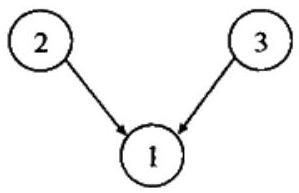
\includegraphics[max width=\textwidth, center]{2025_05_15_6a28331d5e7c993ad07ag-648}

15.前提:因为我喜欢诺兰 • 米尔斯,所以,我在他的回答中听到的是坚强和自信。

假如我不喜欢他,那么我在他的回答中听到的就会是傲慢与恐吓。\\
结论:(并且是下一个论证的前提)第一印象成了自我实现的预言:我们听到的是我们希望听到的东西。

结论:这场访谈带有好感的偏见。\\
20.前提:土著美国人对过去和死亡的信念不应当用于支配政府政策去调查和解释早期美国史前史。只有建立在经验证据上并且能够修正的理论才是科学的。

结论:如果必须在土著美国人理论与科学理论之间做出选择的话,那么就应当首先选择科学理论。

\section*{第1.6节}
5.这不是论证,而是对黑洞是什么的简单说明,它解释了黑洞为何看起来是黑的。

10.这是一个说明,它解释了传统上把丘比特画成瞎子的原因,因而也说明了在爱情的影响下为何那么多的行为是不理智的。

15.表面上,这可以视为一种说明,即说明女孩子为什么害怕科学,会比男孩子发现科学更无趣。但是,这段话还可以用做论证,它支持这样的断定:由于这些态度是学来的,她们的父母和老师可以并且也应当多鼓励女孩子对科学的兴趣。

20.虽然这段话可以作为是对学校中发生的一些情况的说明,但它本质上是一个论证。这段话首先讲明结论,即"美国人的科学教育很成问

题"这个有争议断定,随后给出四个前提来支持这个结论。\\
25.这本质上是说明,是对不被承认的社会和政治环境的阐释,而这种环境决定"黑人孩子倾向于枪击"。这段话还可以直接用于支持对改变这些环境的政策的论证。

\section*{第1.10节}
1.(1)[民主政体的法律一般保护最大多数人的利益,]因为(2)[它们源于大多数的公民,这些公民易于犯错,但他们不会站在自己利益的反面。](3)[相反,寡头政治的法律有助于将财富和权力集中在少数人手中,]因为(4)[从本质上看,寡头政治是由少数人建构起来的。]因此可以断定,一般情况下,(5)[民主政体的立法宗旨比寡头政治的立法宗旨对人类更有益。]\\
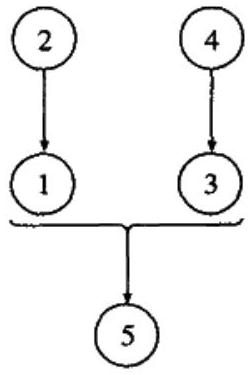
\includegraphics[max width=\textwidth, center]{2025_05_15_6a28331d5e7c993ad07ag-649}

5."……咱们初次会面时,我就对你说过,你是从阿富汗来的,你当时好像还很惊讶哩。"\\
"没问题,一定有人告诉过你。"\\
"根本没有那回事。我当时一看就知道你是从阿富汗来的。由于长久以来的习惯,一系列的思索飞也似的掠过我的脑际,因此在我得出结论时,竟未觉察得出结论所经的步骤。但这中间是有着一定的步骤的。在你这件事上,我的推理过程是这样的:(1)["这一位先生,具有医务工作者的风度,](2)[但却是一副军人气概。]那么,(3)[显见他是个军医。](4) [他刚从热带回来,]因为(5)[他脸色黝黑,](6)[但那并不是他原来的肤色,]因为(7)[他的手腕的皮肤是白相的。](8)[他久病初愈而又历尽艰辛],因为(9)[他面容憔悴。](10)[他左臂受过伤,](11)[现在动作看来还有些僵硬不便。](12)[试问,一个英国的军医在热带地方历尽艰苦,并且

臂部负过伤,这能在什么地方呢?自然只有在阿富汗了。]这一连串的思想,历时不到一秒钟,因此我便脱口说出你是从阿富汗来的,你当时还感到惊讶哩。"

我微笑着说:"听你这样一解释,这件事还是相当简单的呢。"\\
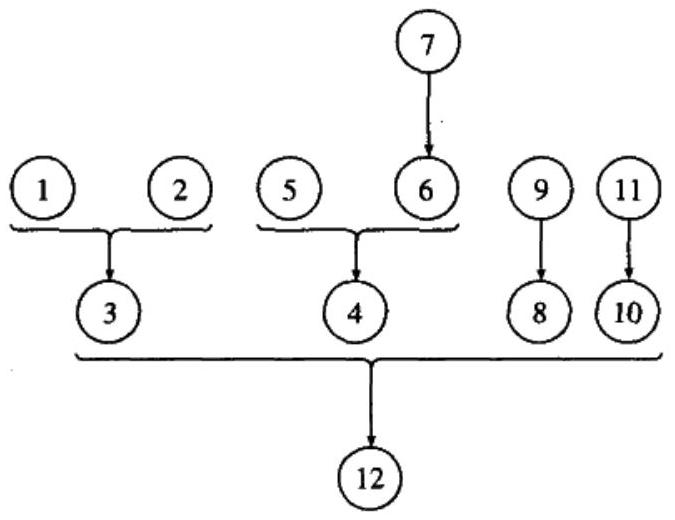
\includegraphics[max width=\textwidth, center]{2025_05_15_6a28331d5e7c993ad07ag-650(1)}

10.(1)[没有东西是可解证的,除非其反面意指一个矛盾。](2)[没有东西可以清楚地可想象地意指一个矛盾。 $]$(3)[无论我们设想为存在物的是什么,我们也可以设想其为不存在物。]因此,(4)[没有其不存在性意指一个矛盾的存在物。]因而,(5)[没有一个其存在性是可解证的存在物。]\\
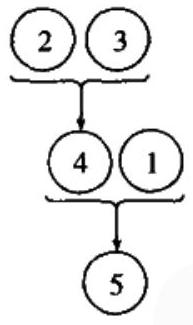
\includegraphics[max width=\textwidth, center]{2025_05_15_6a28331d5e7c993ad07ag-650}

\section*{第1.11节}
1.如果第一位本地人是政客,那么他说的是谎话,并否认自己是政客。如果第一位本地人不是政客,那么他说的是真话,并否认自己是政客。因此,在两种情况下,第一位本地人都否认自己是政客。

由于第二位本地人说第一位本地人否认自己是政客,所以他讲的是真话;因而,他不是政客。

第三位本地人断定第一位本地人是政客。如果第一位本地人是政客,那么第三位本地人说的就是真话,因而他就不是政客。如果第一位本地人不是政客,那么第三位本地人就是撒兓,因而就是政客。因此,第一位和第三位只有一位是政客,因为第二位不是政客,所以三位之中只有一位是政客。

5.由于莱夫提说是斯皮克杀的托瑞利,所以斯皮克的第一和第三句话的意义是相同的,因此,两句话或者都真,或者都假。因为只有一句话是假的,所以这两句话都是真的。

因而,道派的第三句话就是假的,而他的前两句话都真。因此,布切的第三句话为假,而他的前两句话则为真,其中的第二句话暴露了里德是罪犯。\\
[阿拉斯加大学的皮特•M•朗格力(Peter M.Longley)对本题提出了另一种解法。里德几乎是既肯定他们的清白又指控别人。如果他们清白的表白都是假的,那么他们对别人的指控也是假的。但是,没有人做出两句错误陈述,因此他们说他们是清白的必定是真话。所以,里德是罪犯。然而,这种解决方法预设了只有一个人是罪犯。]\\
[这个问题还有一种解法,那是由艾森豪威尔学院(Eisenhower Col- lege)的詹姆士•I•凯姆博尔(James I.Campbell)和罗格斯学院(Rut- gers College)的沃尔特•恰伦(Walter Charen)提出的。道派的第二句话与布切的第三句话相矛盾,所以至少有一句是假的。但是,假如道派的第二句话为假,那么他的第三句话就为真,斯皮克就是罪犯。然而,假如斯皮克是罪犯,那么他的第一句和第三句话就都是假的,因此他不可能是罪犯,道派的第二句话也不可能为假。因而,布切的第三句话必定为假,由此他的第二句话就是真的,而里德就是罪犯。]

10.人们不可能把细绳分配得每个三角形都没有三条同样颜色的边,至少有一个三角形的三条边是同色的。

考虑任何一根钉子,比如我们称做墙 A 上的钉子。从它拉出 5 根细绳,因为只有两种颜色(红和蓝),所以这 5 条细绳中至少有三根是同色的。假设从墙 A 的钉子上扯出的细绳有三根是红的,拉向另三面墙 B、C和 D 。现在,考虑这另三面墙 $\mathrm{B} 、 \mathrm{C}$ 和 D 的钉子形成的三角形。它们肯定不是同色的,所以它们不能都是蓝的,因而它们至少有一根是红的。但是,如果连接 $\mathrm{B} 、 \mathrm{C}$ 和 D 的绳子有一根是红的,那么就必定围成三条红色

边的三角形。(假设连接 B 和 D 的绳子是红的。那么,就会有一个连接 A、 B 和 D 的三根红绳子的三角形,等等。)无论我们从哪一根钉子开始,都不可能避免至少有一个三角形的绳子都是同色的。

11.挑战读者:\\
给出这个有趣问题的答案,会剥夺读者的许多趣味。给出提示就足够了:正确解法(有几种!)都必须从 4 对 4 的称量开始。这样,解答就简单了。

\section*{第 2.3 节}
I.\\
1.指令性\\
5.在这首杰作中,首要的是表达性功能,诗的节奏使作者的情感流露出来。但是,就读者把这首诗视为作者的自传体来说,这里也可以认为有信息性功能。

10.信息性功能。这个报道是正确的,因为阿拉斯加的一小部分穿越了国际日界线。

II.\\
1.这段话主要是信息性用法:它指出美国宪法不允许存在阶级或等级偏好体系。这段话还清晰地表达了大法官哈尔兰对法律面前人人平等的赞同,并引导他人尊重平等。但其引导在这个著名案例中并未获得成功。 (最高法院)应用并确立了种族间"分开但平等"的原则,该原则直到 1954年前一直处于支配地位。 ${ }^{(1)}$

5.这段话的主要功能是表达性的,以激起读者对律师的反感。因为它是空想小说,所以它的很多段落都还具有指令性功能;这里的指令是:摆脱律师!而且,这段话还可以视为向读者传达信息:律师在职业上掩盖和曲解事实。

10.这段话的主要功能是指令性的,埃米尔希望读者不要直到完全清楚明白才做出误事的决定。这段话还可以被认为是信息性的,教导我

\footnotetext{(1)"这个著名案例"指美国法制史上的著名案例——"普菜西诉弗格森案"(1896)。哈尔兰的这段话即在该案审理中发表的意见,他反对具有种族隔离性质的"分开但平等"的原则,但
}们完全地清楚明白对做出明智决定是不可求的。它还有一些表达性功能,对在做出决定之前要弄得完全清楚明白的那些人,作者表示不赞赏。

15.这段话的主要功能可能是信息性的,培根教导说,深人研究哲学就把人带到了宗教那里。它也有指令性功能:作者认为读者应当去信仰宗教,并且如果他们学习哲学,就应当深人研究它,而不是蜻蜓点水。或许,其中对无神论的蔑视也使本段具有一定表达性功能。

20.这段话的主要功能是指令性的。本段中表达的断定涉及"种族概念"的作用,作者对其用法的态度也表达了出来;但作者的目的虽然是使读者少注重种族差异,多关注那些对正常人际互动的挑战。

25.指令性用法。作者讲出了他收到的那些信的信息,但他这里的主要目的是鼓励读者,给他们以反对暴政、中伤和谋杀所需的意志。

III.\\
1.断定讲话者将不接受提名,而且即使当选,他也将不供职。\\
他(Sherman)这里希望打断共和党政治家们对他的提名工作。\\
提供了讲话者不适宜当候选人和他非常直率的证据。\\
5.断定研究需要对已接受信念进行连续不断的反复检验,(作为结论)进一步断定研究对现行实践的批判性。

希望支持和促进研究,激发怀疑态度和批判精神,并告诫那些希望享受研究成果的人,必须容忍对公认原则和现存实践的批判。

为此提供证据:说者主张对基于现有思维和行动的原则和公理进行连续反复检验,主张对现行实践进行批判。

10.断定公民存在所谓的阶层,具有他注意到的特征。\\
希望引起对富人和穷人的仇恨,而赞成中间阶层。\\
提供了说者可能不是富人但几乎肯定又不是穷人的证据。\\
15.断定所有讲宪法权利、言论自由和出版自由的人都是共产主义分子。

希望引起人们敌视主张保护宪法权利、言论自由和出版自由的人,或者敌对要求这种权利的人。

为此提供了证据:说者仇视宪法权利、言论自由、出版自由和共产主义者。

20.断定论及的图画价钱过高,没有价值。

希望引起人们发笑,尤其是嘲笑威斯特勒,希望人们不去买或欣赏威斯特勒的画。

为此提供了证据:说者敌视威斯特勒和他的艺术,其语言诙谐而夸张。

25.断定说者(苏格拉底)知道他的听众被警告不要受他的雄辩力的欺骗,知道他的形象是虚假的,并对此感到惊奇。断定苏格拉底讲的是真话,而他的很多批判者则没有。

希望他的听众(实际上是他在雅典的陪审团)耐心听他的辩护,认为他谦逊,相信他,或许宣告对他的指控罪名不成立。

为此提供了证据:说者论证有力,准备好与他的批判者进行辩论,他的方法非常有雄辩力。

\section*{第2.5节}
1.在如何回答蛀人的信念上有歧见,在对待䘄人的(䁾视)态度上是一致的。

5.在两个人的分开如何影响他们的喜爱或相互如何看待的信念上有歧见。 $a$ 一般地赞同分开,而 $b$ 则好像对之持否定(或许中性)态度,这表明了两人的态度歧见。

15.在对美国政府的价值和性质的信念上有歧见:$a$ 相信它使人蒙羞,而 $b$ 认为,虽然它不完美,但它比那时的其他政府都好。态度上的歧见是:$a$ 不赞赏美国政府,而 $b$ 则赞赏。

20.在对理性可以和将如何运用的信念上有歧见:$a$ 认为,避免危险需要理性,而 $b$ 则认为理性从来都不有利于精神,它常常被人用来反对来自上帝的东西。

态度上的歧见:$a$ 非常赞赏理性,而 $b$ 则非常反对理性及其结果。

\section*{第3.2节}
II.当国会对"使用或携带枪支"犯罪的人提高刑罚时,需要澄清其含义。看来,在这种情况下,较好的精确定义是更能接近国会意欲表达的含义的定义。有人可能辩论说,仅当存在枪支(通过在犯罪过程中使用)加重损失的可能性时,才直接影响犯罪强度。根据这种观点,法官布雷耶的精确定义,设定狭义"携带",会更好些。但实际上,在最高法院的裁

决中得到采用的是法官金斯伯格的精确定义。

\section*{III.}
1.表面上是言辞之争,实际上是实质争论。在歧义短语"伟大的得分手"上,存在言辞争论,戴叶的意思是指得分最多的人,而奈特的意思是本垒打的得分最多的人。除此之外,他们还有实质争论。他们肯定在对罗斯和阿伦的态度上有歧见,因为戴叶认为罗斯是最值得尊重的得分手,而奈特认为阿伦是最值得尊重的得分手。他们或许还在信念上有歧见,对确定谁是最伟大的得分手,维护的标准不同。

5.这仅仅是言辞之争。"业务……良好"是个歧义短语,戴叶是在增加销售额的意义上使用它的,而奈特则是在增加利润的意义上使用的。他们可能是在对所论及公司的态度上有歧见,戴叶持赞赏态度,而奈特则持贬损态度,但这从他们的话语中看得不很清楚。

10.这显然是实质争论。戴叶确认迪克给自己买了辆新车,而奈特则否认。

15.这仅仅是言辞之争。歧义词是"失业者"。戴叶是在比较常见的意义——准备工作并且愿意工作,但没有获得雇用的称职者——上来使用它的。奈特却把同一个词用在了"没有经济收人者"的(有点奇怪的)意义上。

20.这是个机智范例,因为两个分析似乎都合理。一种方案是把它作为明泉的实质争论,戴叶否定命题"奈特应当征询他妻子的意见",而奈特却肯定这个命题。另一种处理方案是把它作为表面言辞争论,但不是实质争论。在这种分析下,(关于那件事)短语"自己的判断"就是有歧义的,戴叶是在无须考虑其他任何人的意见去决定那件事的意义上使用它的,而奈特是在关于那件事的任何决定,包括是否考虑他人的意见,在更广泛的意义上使用它的。在第二种分析下,对奈特是否应该与他妻子商量的信念就存在潜在歧见。

\section*{第3.3节}
I.\\
1.动物,脊椎动物,哺乳动物,猫科动物,野猫,猞猁。\\
5.数,实数,有理数,整数,正整数,质数。

\section*{第 3.4 节}
\section*{I.}
1.(例如)约翰•吉尔古德(John Gielgud),保罗•纽曼(Paul Newman),劳伦斯•奥利维尔(Lawrence Olivier)。

5.(例如)氟,氯,碘。\\
10.(例如)布朗宁,济慈,雪莱。\\
II.\\
1.电影明星(上面使用的例子)。\\
2.卤素(上面使用的例子)。\\
3.维多利亚女王时代的人物(上面使用的例子)。

\section*{第 3.5 节}
I.\\
1.荒谬的\\
5.自我中心\\
10.危险\\
15.征兆\\
II.\\
1.很大的膳食\\
5.年幼的马\\
10.年幼的女性\\
15.很小的马\\
20.雄性马

\section*{第 3.6 节}
II.\\
1.既过宽又过窄。很多天生具有或好或坏地影响他人生活的能力的人都不是天才;也有一些天才,他们并不或好或坏地影响他人的生活。这个定义严重违反规则 3 。

5.䀲涩,违反规则 4。它也没有说清楚变更的本性,即随时间变化,因而它还违反规则1。

10.循环,因为"导致"与"是 $\cdots \cdots$ 原因"同义。违反规则 2 。\\
20.这是个棘手的例子。这个定义可以既是过窄又是过宽的。过窄是因为它只注意到良好状态,而没有注意到健康最常联系到的正常生理状况;它过宽,是因为它引进社会状态,而社会状态一般不被视为处在健康范围内。因此,它违反规则 3 和规则 1 。

III.\\
1.比喻性语言,违反规则 4 。它也没有说出信仰的本质,违反规则1。

5.过宽,因为某些散文也是对这样时刻的记录;还过窄,因为有些 (杰出)诗是悲剧性的;违反规则 3 。它还可以被批评为使用了比喻性语言,违反规则 4 ,虽然这不太明显。

10.过宽,因为有些非常悲观的人也倾向于如此这般;还过窄,因为某些清高自负者并不追慕虚荣和社会交往;违反规则 3 。它还可能被指责违反了规则 1 ,因为它没有说出自负的本质,自负的本质是人物的性格而不是具体明显的行为倾向。

15.过窄;不是所有的政治权力都是用来保障"公众福利"的,当然不是"一切都只是为了公众福利";违反规则 3 。

20.过宽,违反规则 3。在他的《西方哲学史》(History of Western Philosophy)中,罗素批判了这个定义,根据是"教官对待一群新兵,或者制砖者对待一堆砖头,都完全满足杜威(John Dewey)的‘探究’定义"。

30.这个定义初看上去是循环的。然而,它来自维特根斯坦:"即,如果希望理解 ‘意义’ 这个词的用法,那就去查找叫做‘意义的说明’的东西"。通过这种校勘,这个定义就与维特根斯坦的想把意义等同于用法相一致了。请与"铲子就是去挖掘"相比较。

\section*{第4.2节}
I.\\
1.不相干结论一一关心无家可归的人是值得赞扬的,但这与(动物保护组织)所谓的龙虾感到的痛苦不相干。

5.不相干结论。\\
10.人身攻击(诽谤)。

15.诉诸暴力——明显是威胁。\\
II.\\
1.韦尔奇先生真诚地认为对通用电气的攻击是基于虚假前提,他的反应可以视为他对对方前提虚假性的强烈坚持。另一方面,由于他的反应是针对说者作为修女的角色的,它也具有人身攻击(背景谬误)的论证形式。

5.此处同样属于人身攻击论证(背景谬误),其对全国教育协会(在其新闻发布会上的)主张的反对,乃基于设定用于新闻发布的东西不过是设计好为其成员服务的东西。的确,考虑到发布新闻者的组织利益并对此做出更清楚的解释是明智的;但是,只因为发布新闻的目的是服务于组织利益,就认为其主张都是错误的,或发布的事实都是假的,这是不公平的。

\section*{第4.3节}
1.虚假原因("缘出前物")。\\
5.甹题。\\
10.虚假原因。

\section*{第4.4节}
I.\\
1.合成谬误。从部分具有某种特定形状不能推出整体也具有同样形状。

10.合成谬误。\\
II.\\
1.有人可能这样认为,虽然那些部分都具有某些功能,但这不允许推出整体也具有那些功能。根据这种观点,亚里士多德这里就犯了合成谬误。而另一方面,很多人会争论说,我们可以合理地从在某些自然对象中发现的样式推出在其他自然对象中可能有人们期望的相似样式;在这种情况下,这段话就没有谬误。

5.有人可能认为,这段话违犯了人身攻击(背景)谬误,因为它假设了根据教育大臣的孩子的就读学校来怀疑他的忠诚。另一方面,很多人可能争论说,把他的孩子安排到私立学校就读,教育大臣的确不可

避免地损害了公众对他支持公立学校的信任度,因此,这里的推论不是谬误。

III.\\
1.歧义,即文中所讨论的语词的歧义,是这个论争的症结。假如大法官斯卡利亚是对的,那么对"使用"火枪进行严厉处罚的法令的意思就不是给在犯罪中用火枪"进行交换"的人加大制裁力度。另一方面,大法官欧康纳对法令中术语"使用"的看法非常宽泛,因此,火枪的任何作用都会满足"使用"条件。大法官斯卡利亚坚持认为她的论证犯了歧义谬误,因为她的论证把"使用"的意义处理为"任何方式下的使用",而法令应当以其通常意义来理解。这个逻辑问题没有明显的解决结果,它是通过法院投票来解决的。

5.就因为结论受到广泛赞同而相信结论可以接受来说,这里明显包含诉诸情感论证。但是,作者或许仅仅是为了提请注意探究中的普遍存在的非理性因素。

10.这段话使用了虚假原因,也混合着诉诸不当权威谬误。另一方面,作者是在开玩笑,他也嘲弄这样的论证。

15.这个论证可以解释为不包含谬误,亦可解释为包含了一个明显的诉诸暴力论证谬误,即诉诸武力威胁。如果解释为教徒因畏惧上帝发怒导致严厉惩罚而应持有一定的行为方式,那么这个论证就不包含谬误,虽然可以理所当然地质疑它的事实假定。如果解释为由于那些惩罚都是非常可怕的威吓,某些(与上帝发怒没有直接关系的)命题是真的并且应当相信它们为真,那么这个论证就是谬误的,因为这些威吓可能与那些命题的真假无关。或许,这个论证本来就试图在这两方面都起作用。

20.这段幽默之后存在虚假原因谬误。这个问题的答案错误地假设了白天的光是太阳之外的某个东西发出的。

\section*{第5.2节}
1.$S=$ 历史学家;$P=$ 极有天赋、其作品读来如同一流小说的作家。形式:特称肯定命题。

5.$S=$ 富裕、有声望的家庭中的人;$P=$ 富足或显赫的人。形式:特称否定命题。

10.$S=$ 无原创作品的人;$P=$ 可以信赖的评论家。形式:全称否定命题。

\section*{第5.3节}
1.质:肯定;量:特称;\\
主谓项都不周延。\\
5.质:否定;量:全称;\\
主谓项都周延。\\
10.质:肯定;量:全称;\\
主项周延、谓项不周延。

\section*{第5.4节}
1.假定(a)为真,则:\\
(b)与(a)为反对关系,所以(b)为假;\\
(c)与(a)为差等关系,所以(c)为真;\\
(d)与(a)为矛盾关系,所以(d)为假。\\
假定(a)为假,则:\\
(b)与(a)为反对关系,所以(b)真假不定;\\
(c)与(a)为差等关系,所以(c)真假不定;\\
(d)与(a)为矛盾关系,所以(d)为真。

\section*{第 5.5 节}
I.\\
1.没有不顾交通法规的鲁葬驾车人是关心别人的人。与原命题等价。

5.有体力不支的老者是专业摔跤运动员。与原命题等价。\\
II.\\
1.有大学选手不是非职业运动员。\\
5.没有适于作锚的东西是轻于 15 磅的东西。\\
III.\\
1.所有非悲观主义者是非记者。与原命题等价。\\
5.有居民不是公民。与原命题等价。

N.\\
1.假\\
5.假\\
10.假\\
V.\\
1.假\\
5.真假不定\\
10.假

VI.\\
1.真假不定\\
5.假\\
10.真假不定\\
15.假

VI.\\
1.真假不定\\
5.真假不定\\
10.真\\
15.真假不定

\section*{第 5.6 节}
V.\\
第(1)步到第(2)步无效:(1)断定了一个 I 命题为假;(2)断定了与这个命题相应的 O 命题为真。依据传统解释,I 命题与 O 命题为下反对关系,不能同假。因此在这种解释下,如果(1)中的 I 命题为假,(2)中的O命题必定为真。但是,由于I命题与O命题中都有存在含义,在主项对应的类为空时,I 命题与 O 命题可以同假(依据布尔解释)。本题中主项对应的类为空,因为美人鱼是不存在的,因此,由 (1)的假不能推得(2)的真。依据布尔解释,相应的 I 与 O 命题并非下反对关系,但本题中从(1)到(2)的论证却将它们看做下反对关系。

第 5.7 节

5.$S M=0$\\
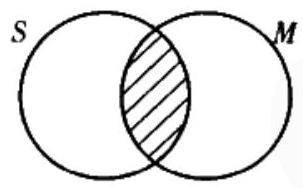
\includegraphics[max width=\textwidth, center]{2025_05_15_6a28331d5e7c993ad07ag-661}

10.$M P=0$\\
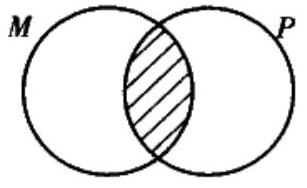
\includegraphics[max width=\textwidth, center]{2025_05_15_6a28331d5e7c993ad07ag-661(1)}

15.$P M \neq 0$\\
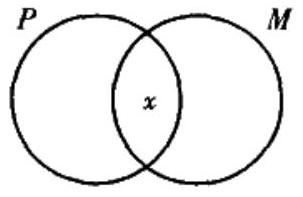
\includegraphics[max width=\textwidth, center]{2025_05_15_6a28331d5e7c993ad07ag-662(1)}

20.$P \bar{M}=0$\\
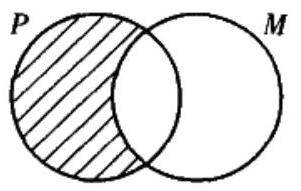
\includegraphics[max width=\textwidth, center]{2025_05_15_6a28331d5e7c993ad07ag-662}

\section*{第6.1节}
5.第1步:结论:有保守派不是倡导高税率的人。\\
第2步:大项:倡导高税率的人。\\
第 3 步:大前提:所有倡导高税率的人是共和党人。\\
第4步:小前提:有共和党人不是保守派。\\
第5步:此三段论的标准形式为:\\
所有倡导高税率的人是共和党人,\\
有共和党人不是保守派,\\
所以,有保守派不是倡导高税率的人。\\
第6步:以上三个命题按顺序分别为 $\mathbf{A} 、 \mathbf{O} 、 \mathbf{O}$ 命题。中项为共和党人,它在大前提中做谓项、在小前提中做主项,因此这个三段论为第四格。其式与格为:AOO-4。\\
10.第1步:结论:没有跑车是家用汽车。\\
第2步:大项:家用汽车。\\
第3步:大前提:所有家用汽车是以中档速度运行的车。\\
第4步:小前提:没有跑车是以中档速度运行的车。\\
第5步:此三段论的标准形式为:\\
所有家用汽车是以中档速度运行的车,\\
没有跑车是以中档速度运行的车,\\
所以,没有跑车是家用汽车。\\
第6步:以上三个命题按顺序分别为 $\mathbf{A} 、 \mathbf{E} 、 \mathbf{E}$ 命题。中项为以中档速度运行的车,它在大前提和小前提中都做谓项,因此这个三段论为第二格。其式与格为:AEE-2。

\section*{第6.2节}
5.可以反驳这个无效论证的反例之一是:\\
所有独角兽是哺乳动物,所以,有哺乳动物不是动物,因为没有动物是独角兽。

10.可以反驳这个无效论证的反例之一是:\\
所有方的圆是圆,并且所有方的圆是方,因此有些圆是方。

\section*{第6.3节}
I.

5.没有 $P$ 是 $M$ ,有 $M$ 是 $S$ ,\\
$\therefore$ 有 $S$ 不是 $P$ 。\\
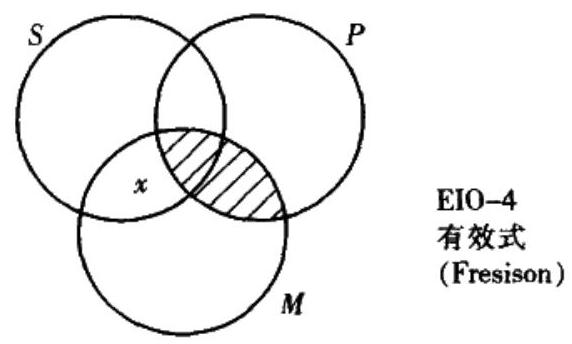
\includegraphics[max width=\textwidth, center]{2025_05_15_6a28331d5e7c993ad07ag-663}

10.有 $P$ 是 $M$ ,所有 $M$ 是 $S$ ,\\
$\therefore$ 有 $S$ 是 $P$ 。\\
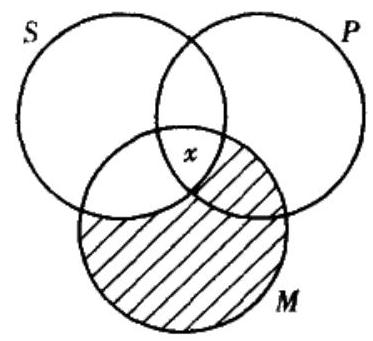
\includegraphics[max width=\textwidth, center]{2025_05_15_6a28331d5e7c993ad07ag-663(2)}

IAI-4有效式 (Dimaris)

15.没有 $M$ 是 $P$ ,有 $S$ 是 $M$ ,\\
$\therefore$ 有 $S$ 不是 $P$ 。\\
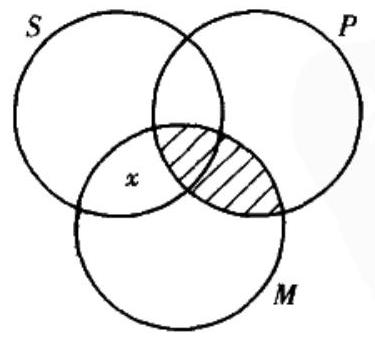
\includegraphics[max width=\textwidth, center]{2025_05_15_6a28331d5e7c993ad07ag-663(1)}

EIO-1有效式 (Ferio)

II.

1.有改革者是狂徒,所有改革者是理想主义者,\\
$\therefore$ 有理想主义者是狂徒。\\
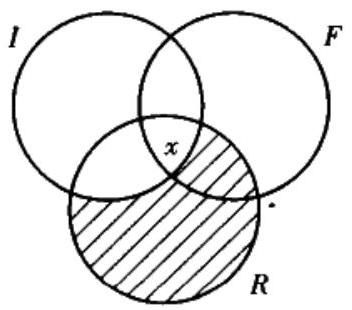
\includegraphics[max width=\textwidth, center]{2025_05_15_6a28331d5e7c993ad07ag-664(1)}

IAI-3\\
有效式 (Disamis)

5.没有游艇是水下船只,所有水下船只是潜水艇, $\therefore$ 没有潜水艇是游艇。\\
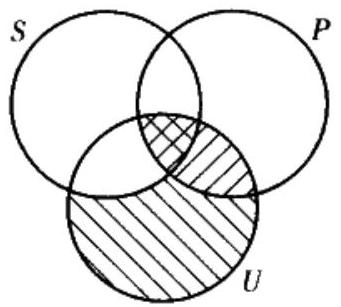
\includegraphics[max width=\textwidth, center]{2025_05_15_6a28331d5e7c993ad07ag-664}

EAE-4无效式

10.所有工人领导是真正的自由党人,没有怯懦者是真正的自由党人, $\therefore$ 没有怯懦者是工人领导。\\
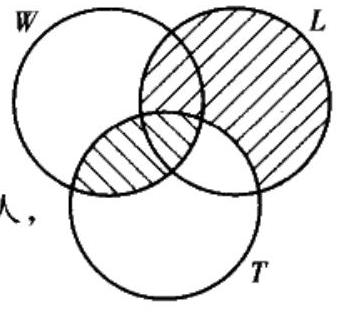
\includegraphics[max width=\textwidth, center]{2025_05_15_6a28331d5e7c993ad07ag-664(2)}

AEF-2\\
有效式 (Camestres)

\section*{第6.5节}
I.\\
5.违反了规则 3 ,犯了"小项不当周延"的谬误。\\
10.违反了规则 3 ,犯了"大项不当周延"的谬误。\\
15.违反了规则 3 ,犯了"小项不当周延"的谬误。\\
II.\\
5.违反了规则 6,犯了"存在谬误"。\\
10.违反了规则 3 ,犯了"小项不当周延"的谬误。\\
III.\\
5.违反了规则 3 ,犯了"小项不当周延"的谬误。\\
10.违反了规则 1,犯了"四项"的谬误。(其中"喜欢它的人"是歧义词,在结论中的含义与在前提中的含义截然不同。)

\section*{第6.6节}
5.显然,此题可能是第一格的 AII-1 式,有效。其中只有一个项周延,并且只出现一次,也可能是第三格的 AII-3(IAI-3 也一样),有效,其中只有一个项周延,并且只出现一次。还可能是第四格的 IAI-4,有效,其中也只有一个项周延,并且只出现一次。但不能是中项在两个前提中都做谓项,即不可能是第二格。试想,在第二格中,为了不违反规则 2 ,即中项在前提中至少周延一次,前提之一必为否定命题。这样,根据规则 5 ,结论中谓项必须周延,即结论必为否定命题。因此,在只有一个项周延并且只周延一次的情况下,第二格中周延的项必须在结论中。而如果周延的项只出现一次,就违反了规则 3 ,因为这个项在结论中周延,在前提中却不周延。

10.没有满足本题要求的三段论。如果中项在前提中两次都周延,那么,在第一格中,小前提必为否定,而(根据规则5)结论也必为否定,所以根据规则 3 ,大前提也必为否定,违反规则 4 。在第二格中,两个前提均为否定命题,违反规则 4 。在第三格中,两个前提必然都为全称命题,据规则 3 ,小前提必为否定,根据规则 5 ,结论为否定命题——再根据规则 3 大前提也必为否定,违反规则 4 。在第四格中,大前提必为否定,根据规则 3 ,大前提为全称命题,因此(根据规则 3 )小前提为否定命题,也违反规则 4 。

\section*{第7.2节}
5.令 $E=$ 爆炸物;\\
$F=$ 容易点燃的东西[注意,容易点燃的东西(flammable)和易燃物(inflammable)为同义词];\\
$S=$ 安全的东西;\\
则原来的三段论可以翻译为如下的标准形式:\\
所有 $E$ 是 $F$ ,\\
没有 $F$ 是 $S$ ,\\
所以,没有 $S$ 是 $E$ 。\\
根据这个三段论(Camenes 式)的文恩图,可知它是有效式。\\
10.令 $O=$ 超过 6 英尺的东西;

\section*{$U=$ 有用的东西;}
则原来的三段论可以翻译为如下的标准形式:\\
所有 $O$ 是 $D$ ,\\
没有 $D$ 是 $U$ ,\\
所以,没有 $U$ 是 $O$ 。\\
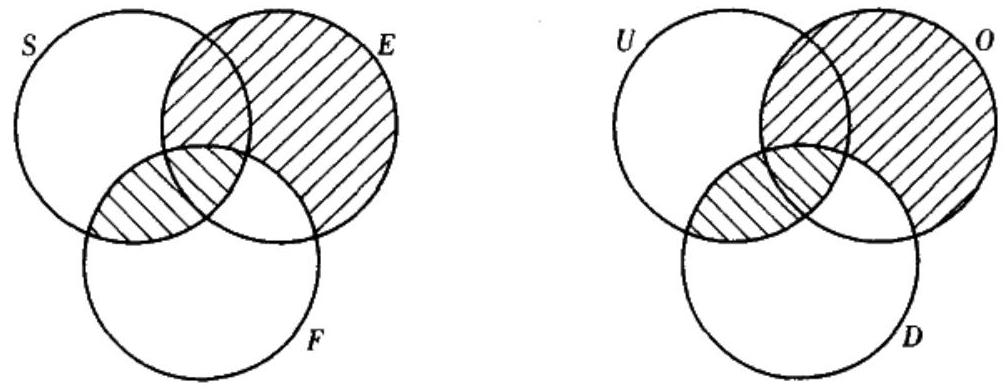
\includegraphics[max width=\textwidth, center]{2025_05_15_6a28331d5e7c993ad07ag-666}

根据这个三段论(Camenes 式)的文恩图,可知它是有效式。

\section*{第7.3节}
5.所有 Junkos 是钱能买到的最好的东西。\\
10.没有面朝太阳的人是看到自己影子的人。\\
15.没有护卫军候选人是受土耳其青年拥护的人。(或者:没有土耳其青年是拥护护卫军候选人的人。)

20.所有博爱者是虔诚者。\\
25.所有灵活的答案是可以避免非议的东西。

\section*{第7.4节}
I.\\
5.所有她发表意见的场合都是她被问到的场合。\\
10.没有自由争论的时间是解决问题的时间。\\
II.\\
5.所有破产的公司(B)是负担不起债务利息的公司(U)。\\
巴塞罗那运输公司( $T$ )是负担不起债务利息的公司。\\
$\therefore$ 巴塞罗那运输公司是破产的公司。\\
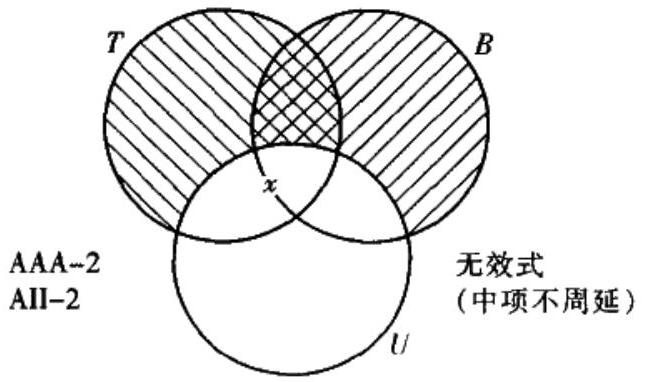
\includegraphics[max width=\textwidth, center]{2025_05_15_6a28331d5e7c993ad07ag-667(2)}

10.没有金子 $(G)$ 是贱金属 $(B)$ 。\\
有贱金属是发光的东西 $(T)$ 。\\
$\therefore$ 有发光的东西不是金子。\\
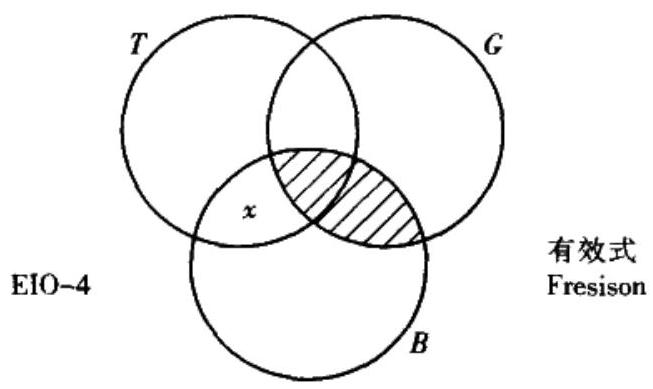
\includegraphics[max width=\textwidth, center]{2025_05_15_6a28331d5e7c993ad07ag-667}

15.没有真正客观的人(O)是会犯错误的人(L)。\\
所有会犯错误的人是不顾事实的人(I)。\\
$\therefore$ 没有不顾事实的人是真正客观的人。\\
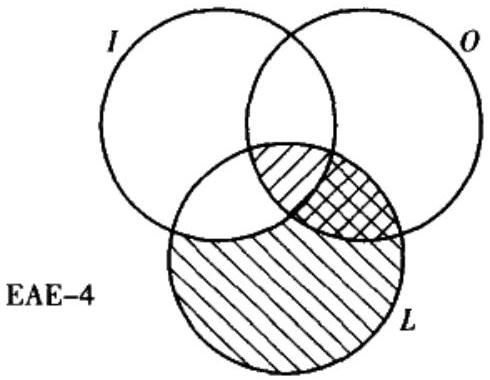
\includegraphics[max width=\textwidth, center]{2025_05_15_6a28331d5e7c993ad07ag-667(1)}

无效式\\
(小项不当周延)

20.所有对工程师有意义的东西 $(E)$ 都是近似值 $(A)$ 。\\
没有近似值是无理数( $I$ )。\\
$\therefore$ 没有无理数是对工程师有意义的东西。\\
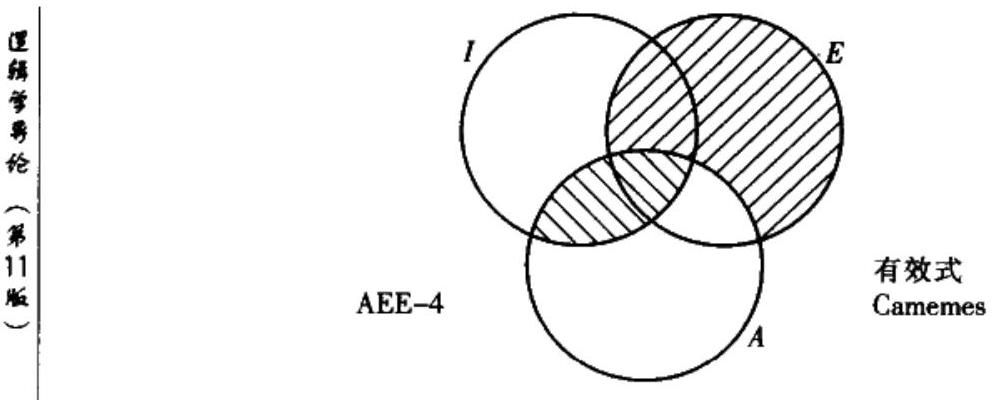
\includegraphics[max width=\textwidth, center]{2025_05_15_6a28331d5e7c993ad07ag-668(2)}

25.所有酗酒的人( $E$ )是负债人(D)。\\
有酗酒的人不是失业者(U)。\\
$\therefore$ 有失业者不是负债人。\\
\includegraphics[max width=\textwidth, center]{2025_05_15_6a28331d5e7c993ad07ag-668}

无效式 (大项不当周延)

30.所有纠察员出现的地方 $(P)$ 是有罢工的地方 $(S)$ 。\\
这个工厂 $(F)$ 是纠察员出现的地方。\\
$\therefore$ 这个工厂是有罢工的地方。\\
\includegraphics[max width=\textwidth, center]{2025_05_15_6a28331d5e7c993ad07ag-668(1)}

35.所有有效三段论( $V$ )是中项至少在一个前提中周延的三段论 (D)。

这个三段论 $(T)$ 是中项至少在一个前提中周延的三段论。\\
$\therefore$ 这个三段论是有效三段论。\\
\includegraphics[max width=\textwidth, center]{2025_05_15_6a28331d5e7c993ad07ag-669}

40.所有出席的人( $P$ )都是有工作的人( $E$ )。\\
所有会员( $M$ )都是出席的人。\\
$\therefore$ 所有会员都是有工作的人。\\
\includegraphics[max width=\textwidth, center]{2025_05_15_6a28331d5e7c993ad07ag-669(2)}

45.所有他生病的时候( $S$ )都是他怨天尤人的时候( $C$ )。\\
现在 $(T)$ 不是他生病的时候。\\
$\therefore$ 现在不是他怨天尤人的时候。\\
\includegraphics[max width=\textwidth, center]{2025_05_15_6a28331d5e7c993ad07ag-669(1)}

图 7.4-II-45\\
50.所有高于 300 英尺的建筑(B)是摩天大楼(S)。\\
有现代建筑(E)不是摩天大楼。\\
$\therefore$ 有现代建筑不是高于 300 英尺的建筑。\\
\includegraphics[max width=\textwidth, center]{2025_05_15_6a28331d5e7c993ad07ag-670(1)}

\section*{第 7.5 节}
5.第一种省略体。\\
所有肉身 $(F)$ 都是被动的、荷尔蒙与性征的玩弄对象、无休止欲望的牺牲品 $(P)$ 。

所有男人( $M$ )是肉身。\\
$\therefore$ 所有男人是被动的、荷尔蒙与性征的玩弄对象、无休止欲望的牺 583牲品。\\
\includegraphics[max width=\textwidth, center]{2025_05_15_6a28331d5e7c993ad07ag-670}

有效式 Barbara

\section*{10.第一种省略体。}
没有这样的生物(A)——其行为既受外部压力的控制,也受其内在需要的制约——是拥有哲学意义上自由的生物 $(F)$ 。

所有人 $(P)$ 是这样的生物——其行为既受外部压力的控制,也受其内在需要的制约。\\
$\therefore$ 没有人是拥有哲学意义上自由的生物。\\
这是个有效的省略三段论,其中大前提可表述为:"没有拥有哲学意义上自由的生物是既受外部压力的控制,也受其内在需要的制约的生物。"\\
\includegraphics[max width=\textwidth, center]{2025_05_15_6a28331d5e7c993ad07ag-671(1)}

15.第三种省略体。\\
没有为金钱卖命的人( $M$ )是能为上帝服务的人( $G$ )。\\
亨利( $H$ )是为金钱卖命的人。\\
$\therefore$ 亨利不是能为上帝服务的人。\\
\includegraphics[max width=\textwidth, center]{2025_05_15_6a28331d5e7c993ad07ag-671}

20.第一种省略体。\\
所有了解孩子的父亲( $K$ )都是明智的父亲( $W$ )。\\
他 $(H)$ 是了解孩子的父亲。\\
$\therefore$ 他是明智的父亲。\\
\includegraphics[max width=\textwidth, center]{2025_05_15_6a28331d5e7c993ad07ag-671(2)}\\
"他是一个了解孩子的父亲。"\\
25.第一种省略体。\\
使核战争变得容易的武器( $E$ )是可能最危险的武器( $D$ )。\\
毁灭性最弱的核武器( $L$ )是使核战争变得容易的武器。\\
$\therefore$ 毁灭性最弱的核武器是可能最危险的武器。\\
\includegraphics[max width=\textwidth, center]{2025_05_15_6a28331d5e7c993ad07ag-672}

30.第二种省略体。\\
所有剧场可能存在的时间 $(T)$ 都是可能做如下装扮的时间 $(P)-$假装有一些自己实际上没有的动机和能力,或假装自己的动机达到了实际上并不具有的强度,以及假装自己的能力达到了实际上并不具有的水平。

所有时间(A)都是剧场可能存在的时间。\\
$\therefore$ 所有时间都是可能做如下装扮的时间——假装有一些自己实际上没有的动机和能力,或假装自己的动机达到了实际上并不具有的强度,以及假装自己的能力达到了实际上并不具有的水平。\\
\includegraphics[max width=\textwidth, center]{2025_05_15_6a28331d5e7c993ad07ag-672(1)}

\section*{第7.6节}
I.\\
5.(1')所有有意义的诗歌( $I$ )是受到高品位者欢迎的诗歌( $P$ )。\\
$\left(4^{\prime}\right)$ 没有矫揉造作的诗歌 $(A)$ 是受到高品位者欢迎的诗歌。\\
$\left(2^{\prime}\right)$ 所有现代诗歌 $(M)$ 都是矫揉造作的诗歌。\\
(5')所有谈及"肥皂泡"(S)的诗歌是现代诗歌。\\
$\left(3^{\prime}\right)$ 你的所有诗歌(Y)是谈及"肥皂泡"的诗歌。\\
$\therefore$ 你的诗歌没有是有意义的诗歌。

所有 $I$ 是 $P$ ,没有 $A$ 是 $P$ , $\therefore$ 没有 $A$ 是 $I$ 。\\
\includegraphics[max width=\textwidth, center]{2025_05_15_6a28331d5e7c993ad07ag-673(4)}

没有 $A$ 是 $I$ ,没有 $M$ 是 $A$ , $\therefore$ 没有 $M$ 是 $I$ 。\\
\includegraphics[max width=\textwidth, center]{2025_05_15_6a28331d5e7c993ad07ag-673(2)}

没有 $M$ 是 $I$ ,所有 $S$ 是 $M$ , $\therefore$ 没有 $S$ 是 $I$ 。\\
\includegraphics[max width=\textwidth, center]{2025_05_15_6a28331d5e7c993ad07ag-673(5)}

没有 $S$ 是 $I$ ,所有 $Y$ 是 $S$ , $\therefore$ 没有 $Y$ 是 $I$ 。\\
\includegraphics[max width=\textwidth, center]{2025_05_15_6a28331d5e7c993ad07ag-673(3)}

II.\\
1.(1')所有读泰晤士报的人( $T$ )是受过良好教育的人( $W$ )。\\
$\left(3^{\prime}\right)$ 没有不会阅读的生物 $(C)$ 是受过良好教育的人。\\
$\left(2^{\prime}\right)$ 所有剌猬 $(H)$ 是不会阅读的生物。\\
$\therefore$ 没有刺猬是读泰晤士报的人。

所有 $T$ 是 $W$ ,没有 $C$ 是 $W$ , $\therefore$ 没有 $C$ 是 $T_{\text {。 }}$\\
\includegraphics[max width=\textwidth, center]{2025_05_15_6a28331d5e7c993ad07ag-673}

没有 $C$ 是 $T$ ,所有 $H$ 是 $C$ , $\therefore$ 没有 $H$ 是 $T_{\text {。 }}$\\
\includegraphics[max width=\textwidth, center]{2025_05_15_6a28331d5e7c993ad07ag-673(1)}

5.$\left(2^{\prime}\right)$ 这些连锁论证 $(S)$ 是不按标准的顺序排列的题目 $(N)$ 。\\
(4')没有不按标准顺序排列的题目是我会做的题目(U)。\\
$\left(1^{\prime}\right)$ 所有我没有抱怨的题目 $(G)$ 是我会做的题目。\\
$\left(5^{\prime}\right)$ 所有让我觉得头痛的题目 $(H)$ 是我没有抱怨的题目。\\
$\left(3^{\prime}\right)$ 所有容易的题目( $E$ )是不会让我觉得头痛的题目。\\
$\therefore$ 这些连锁论证不是容易的题目。\\
\includegraphics[max width=\textwidth, center]{2025_05_15_6a28331d5e7c993ad07ag-674(2)}

所有 $G$ 是 $U$ ,没有 $S$ 是 $U$ , $\therefore$ 没有 $S$ 是 $G$ 。\\
\includegraphics[max width=\textwidth, center]{2025_05_15_6a28331d5e7c993ad07ag-674(1)}

没有 $S$ 是 $G$ ,所有 $H$ 是 $G$ , $\therefore$ 没有 $S$ 是 $H$ 。\\
\includegraphics[max width=\textwidth, center]{2025_05_15_6a28331d5e7c993ad07ag-674(3)}

没有 $S$ 是 $H$ ,所有 $E$ 是 $H$ , $\therefore$ 没有 $S$ 是 $E$ 。\\
\includegraphics[max width=\textwidth, center]{2025_05_15_6a28331d5e7c993ad07ag-674}

\section*{第 7.7 节}
5.否定前件的谬误,无效。\\
10.纯假言复合三段论,无效。\\
15.析取三段论,有效。\\
20.纯假言复合三段论,有效。\\
25.混合假言三段论和分离律,有效。\\
30.混合假言三段论和分离律,有效。\\
35.混合假言三段论和分离律,有效。

\section*{第 7.8 节}
5.反驳这个二难推论的关键在于揭示"超出"(going beyond)一词的双关性。"超出"可以表示"逻辑上超出,得到原来命题并不蕴涵的结论",也可以表示"心理上超出,得到原来没有掌握的新知"。这样一来,根据"超出"一词有意的混淆,直击二难推论的任何一角就能进行反驳。这里可以构造一个合理的不可辩驳的反例。

10.对于这个二难推论,采用绕过(或避开)死角法的方法比较简单,因为在圣人与恶徒之间是一个不间断的连续统,人正处于这个连续统之中。直击一角法也可以,即指出即使很坏的人,也有可能通过加强法制的方式限制其行为。在题中给定的二难推论之外,也可以构造一个看似似是而非但却不可辩驳的反例。

15.对于这个二难推论,绕过(或避开)死角法是不可能的。可以采用直击一角的方法,或者指出(a)即使知道改变不会比现在更糟,甚至会更好,但还是希望保持现状,这只是惯性使然、安于现状——只是"担心改变太麻烦,不值得"。(b)即使知道改变可能不比现在更好,甚至更糟,但还是想改变,这是因为感到无聊和厌倦——只是想"来点儿变化吧"。可见这是心理上的问题而非政治或道德问题,而原来的二难推论本身显然是心理上的。此处可以用一个普通的反例反驳它:如果要保持现状,就是不想得到更好的东西;如果想要改变,就是不想阻止更坏的情况发生。

20.对第一个二难推论,不能用绕过(或避开)死角法,至少如果 "超出原来的含义"被理解为"与原来的含义不同"时不能避开。但直击第一个角比较容易,特别是按照弗雷格的理论一一将含义与指称区分开来。对于第二个角,也可以加以直击,一个可行的方法是从澄清双关语的角度考虑,另一个是从分析改进这些词(或概念)合理目的的角度考虑。可以在这个二难之外构造出普通但不可辩驳的反例。对于第二个角,可以指出,一个新词的正确使用应当采用,或者简化为清晰的说明。也就是说,直击第一个角,通常可以在原来的二难推论之外构造一个不可辩驳的反例。

25.对于这个二难推论,绕过(或避开)死角法是不可能的,但直击任何一个角都可以。想要拥有和平,不能鼓励竞争精神的说法是可质疑的;可以争辩说,竞争精神所带来的生产力本身就为满足和平的要求所需要。或者指出如果想要取得进步,就必须鼓励竞争精神的说法也是可质疑的,因为竞争中的合作可以带来更持久更令人满意的进步。

30.此题采用绕过(或避开)死角法的方法为宜。在薪水的连续统中,当然有一个既不会太高也不会过低的范围(尽管可能很狭窄)。也可以直击任何一个角,只是合理性程度有些区别。如果要的薪水"太高",招聘者可能会觉得应聘者值得他们付出更多的薪水。如果要的薪水"太低",可以表现出应聘者得到这份工作的热情,并确信招聘者会很快给他加薪。

\section*{第8.2节}
I.1.真 5.真 10.真 15.假 20.真 25.假\\
II.1.真 5.假 10.真 15.真 20.假 25.假\\
III.1.真 5.真 10.假 15.假 20.真 25.假\\
N.1.I.~L 5.~I.~L 10.~~(EVJ)\\
15.$\sim I \vee L$ 20.$(I \cdot E) \vee \sim(J \cdot S)$\\
25.$(L \cdot E) \cdot(S \cdot J)$

\section*{第8.3节}
I.1.真 5.假 10.真 15.假 20.假 25.真\\
II.1.真 5.假 10.假 15.真 20.假 25.真\\
III.1.$A \supset(B \supset C) \quad$ 5.$(A \cdot B) \supset C$\\
10.~[Aつ $(B \cdot C)]$ 15.$B \supset(A \vee C)$\\
20.$B \vee C$ 25.$(\sim C \cdot \sim D) \supset(\sim B \vee A)$

\section*{第8.4节}
I.e. 10 是 $e$ 的特征形式。\\
o. 3 以 $o$ 为代人例, 24 是 $o$ 的特征形式。\\
II.\\
1.

\begin{center}
\begin{tabular}{|l|l|l|l|l|l|}
\hline
$p$ & $q$ & $p \supset q$ & $\sim q$ & $\sim p$ & $\sim q \supset \sim p$ \\
\hline
T & T & T & F & F & T \\
\hline
T & F & F & T & F & F \\
\hline
F & T & T & F & T & T \\
\hline
F & F & T & T & T & T \\
\hline
\multicolumn{6}{|l|}{有效} \\
\hline
\end{tabular}
\end{center}

5.

\begin{center}
\begin{tabular}{|ccc|}
\hline
$p$ & $q$ & $p \supset q$ \\
\hline
T & T & T \\
T & $F$ & F \\
F & T & T \\
F & F & T \\
\hline
无效(第二行表明了这一点) &  &  \\
\hline
\end{tabular}
\end{center}

10.

\begin{center}
\begin{tabular}{|ccc|}
\hline
$p$ & $q$ & $p \cdot q$ \\
\hline
T & T & T \\
T & F & F \\
F & T & F \\
F & F & F \\
\hline
有效 &  &  \\
\hline
\end{tabular}
\end{center}

15.

\begin{center}
\begin{tabular}{|l|l|l|l|l|l|l|l|l|}
\hline
$p$ & $q$ & $r$ & $q$ つr & $p \supset(q \supseteq r)$ & $p$ つr & $q \supset(p \supset r)$ & $p \vee q$ & $(p \vee q) \supset r$ \\
\hline
T & T & T & T & T & T & T & T & T \\
\hline
T & T & F & F & F & F & F & T & F \\
\hline
T & F & T & T & T & T & T & T & T \\
\hline
T & F & F & T & T & F & T & T & F \\
\hline
F & T & T & T & T & T & T & T & T \\
\hline
F & T & F & F & T & T & T & T & F \\
\hline
F & F & T & T & T & T & T & F & T \\
\hline
F & F & F & T & T & T & T & F & T \\
\hline
\multicolumn{9}{|l|}{无效(第四和第六行表明了这一点)} \\
\hline
\end{tabular}
\end{center}

20.

590

\begin{center}
\begin{tabular}{|l|l|l|l|l|l|l|l|l|l|l|}
\hline
$p$ & $q$ & $r$ & $s$ & $p \cdot q$ & $p \supset q$ & $(p \cdot q) \supset r$ & $r \supset s$ & $p \supset(r \supset s)$ & \begin{tabular}{l}
( $p \supset q$ )• \\
$[(p \cdot q) \supset r]$ \\
\end{tabular} & $p \supset s$ \\
\hline
T & T & T & T & T & T & T & T & T & T & T \\
\hline
T & T & T & F & T & T & T & F & F & T & F \\
\hline
T & T & F & T & T & T & F & T & T & F & T \\
\hline
T & T & F & F & T & T & F & T & T & F & F \\
\hline
T & F & T & T & F & F & T & T & T & F & T \\
\hline
T & F & T & F & F & F & T & F & F & F & F \\
\hline
T & F & F & T & F & F & T & T & T & F & T \\
\hline
T & F & F & F & F & F & T & T & T & F & F \\
\hline
F & T & T & T & F & T & T & T & T & T & T \\
\hline
F & T & T & F & F & T & T & F & T & T & T \\
\hline
F & T & F & T & F & T & T & T & T & T & T \\
\hline
F & T & F & F & F & T & T & T & T & T & T \\
\hline
F & F & T & T & F & T & T & T & T & T & T \\
\hline
F & F & T & F & F & T & T & F & T & T & T \\
\hline
F & F & F & T & F & T & T & T & T & T & T \\
\hline
F & F & F & F & F & T & T & T & T & T & T \\
\hline
\multicolumn{11}{|l|}{有效} \\
\hline
\end{tabular}
\end{center}

III.\\
1.$(A \vee B) \supset(A \cdot B)$\\
$(p \vee q) \supset(p \cdot q)$\\
$A \vee B$\\
其特征形式为:\\
$p \vee q$\\
$\therefore A \cdot B$\\
$\therefore p \cdot q$

\begin{center}
\begin{tabular}{|l|l|l|l|l|}
\hline
$p$ & $q$ & $p \vee q$ & $p \cdot q$ & $(p \vee q) \supset(p \cdot q)$ \\
\hline
T & T & T & T & T \\
\hline
' T & F & T & F & F \\
\hline
F & T & T & F & F \\
\hline
F & F & F & F & T \\
\hline
\multicolumn{5}{|c|}{有效} \\
\hline
\end{tabular}
\end{center}

5.$(I \vee J) \supseteq(I \cdot J)$\\
$(p \vee q) \supset(p \cdot q)$\\
$\sim(I \vee J)$\\
其特征形式为:\\
$\sim(p \vee q)$\\
$\therefore \sim(I \cdot J)$\\
$\therefore \sim(p \cdot q)$

\begin{center}
\begin{tabular}{|l|l|l|l|l|l|l|}
\hline
$p$ & $q$ & $p \vee q$ & $p \cdot q$ & $(p \vee q) \supset(p \cdot q)$ & $\sim(p \vee q)$ & $\sim(p \cdot q)$ \\
\hline
T & T & T & T & T & F & F \\
\hline
T & F & T & F & F & F & T \\
\hline
F & T & T & F & F & F & T \\
\hline
F & F & F & F & T & T & T \\
\hline
\multicolumn{7}{|l|}{有效(注意:这儿没犯否定前件谬误!)} \\
\hline
\end{tabular}
\end{center}

10.Uつ( $V \vee W$ )\\
$p \supset(q \vee r)$\\
591\\
$(V \cdot W) \supset \sim U$\\
其特征形式为:\\
$(q \cdot r) \supset \sim p$\\
$\therefore \sim U$\\
$\therefore \sim p$

\begin{center}
\begin{tabular}{|l|l|l|l|l|l|l|l|}
\hline
$p$ & $q$ & $r$ & $q \vee r$ & $p \supset(q \vee r)$ & $q \cdot r$ & $\sim p$ & ( $q \cdot r$ ) \\
\hline
T & T & T & T & T & T & F & F \\
\hline
T & T & F & T & T & F & F & T \\
\hline
T & F & T & T & T & F & F & T \\
\hline
T & F & F & F & F & F & F & T \\
\hline
F & T & T & T & T & T & T & T \\
\hline
F & T & F & T & T & F & T & T \\
\hline
F & F & T & T & T & F & T & T \\
\hline
F & F & F & F & T & F & T & T \\
\hline
\multicolumn{8}{|l|}{无效(第二和第三行表明了这一点)} \\
\hline
\end{tabular}
\end{center}

IV.

1.$A \supset(B \cdot C)$\\
$\sim B$\\
$\therefore \sim A$\\
$p \supset(q \cdot r)$\\
其特征形式为:$\sim q$\\
$\therefore \sim p$

\begin{center}
\begin{tabular}{|l|l|l|l|l|l|l|}
\hline
$p$ & $q$ & $r$ & $q \cdot r$ & $p \supset(q \cdot r)$ & $\sim q$ & $\sim p$ \\
\hline
T & T & T & T & T & F & F \\
\hline
T & T & F & F & F & F & F \\
\hline
T & F & T & F & F & T & F \\
\hline
T & F & F & F & F & T & F \\
\hline
F & T & T & T & T & F & T \\
\hline
F & T & F & F & T & F & T \\
\hline
F & F & T & F & T & T & T \\
\hline
F & F & F & F & T & T & T \\
\hline
\multicolumn{7}{|l|}{有效} \\
\hline
\end{tabular}
\end{center}

5.

\begin{center}
\begin{tabular}{lll}
$M \supset(N \supset O)$ &  & $p \supset(q \supset r)$ \\
$N$ & 其特征形式为: & $q$ \\
$\therefore O \supset M$ &  & $\therefore r \supset p$ \\
\end{tabular}
\end{center}

\begin{center}
\begin{tabular}{|l|l|l|l|l|l|}
\hline
$p$ & $q$ & $r$ & $q \supset r$ & $p \supset(q \supset r)$ & $r \supset p$ \\
\hline
T & T & T & T & T & T \\
\hline
T & T & F & F & F & T \\
\hline
T & F & T & T & T & T \\
\hline
T & F & F & T & T & T \\
\hline
F & T & T & T & T & F \\
\hline
F & T & F & F & T & T \\
\hline
F & F & T & T & T & F \\
\hline
F & F & F & T & T & T \\
\hline
\multicolumn{6}{|c|}{无效(第五行表明了这一点)} \\
\hline
\end{tabular}
\end{center}

10.可以符号化为:

$$
\begin{aligned}
& C \supset(I \cdot D) \\
& (I \vee D) \supset B \\
& \therefore C \supset B
\end{aligned}
$$

其特征形式为:

$$
\begin{aligned}
& p \supset(q \cdot r) \quad \text { 有效 } \\
& (q \vee r) \supset s \\
& \therefore p \supset s
\end{aligned}
$$

\section*{第8.5节}
I.\\
1.$c$ 是 1 的特征形式。\\
5.$c$ 以 5 为代人例,且 $i$ 是 5 的特征形式。\\
10.$e$ 以 10 为代人例。\\
\includegraphics[max width=\textwidth, center]{2025_05_15_6a28331d5e7c993ad07ag-680}\\
II.\\
1.

\begin{center}
\begin{tabular}{|l|l|l|l|l|}
\hline
$p$ & $q$ & $p \supset q$ & $p \supset(p \supset q)$ & $[p \supset(p \supset q)] \supset q$ \\
\hline
T & T & T & T & T \\
\hline
T & F & F & F & T \\
\hline
F & T & T & T & T \\
\hline
F & F & T & T & F \\
\hline
\multicolumn{5}{|c|}{偶真式} \\
\hline
\end{tabular}
\end{center}

5.

\begin{center}
\begin{tabular}{|l|l|l|l|l|l|}
\hline
$p$ & $q$ & $\sim q$ & $q \cdot \sim q$ & $p \supset(q \cdot \sim q)$ & $p \supset[p \supset(q \cdot \sim q)]$ \\
\hline
T & T & F & F & F & F \\
\hline
T & F & T & F & F & F \\
\hline
F & T & F & F & T & T \\
\hline
F & F & T & F & T & T \\
\hline
\multicolumn{6}{|l|}{偶真式} \\
\hline
\end{tabular}
\end{center}

10.偶真式。最后一栏为:TTTTTTTTTTFFTTFT\\
III.\\
1.

\begin{center}
\begin{tabular}{|l|l|l|l|l|l|l|}
\hline
$p$ & $q$ & $p \supset q$ & $\sim q$ & $\sim p$ & $\sim q \supset \sim p$ & $(p \supset q) \equiv(\sim q \supset \sim p)$ \\
\hline
T & T & T & F & F & T & T \\
\hline
T & F & F & T & F & F & T \\
\hline
F & T & T & F & T & T & T \\
\hline
F & F & T & T & T & T & T \\
\hline
\multicolumn{7}{|l|}{重言式} \\
\hline
\end{tabular}
\end{center}

5.

\begin{center}
\begin{tabular}{|l|l|l|l|l|}
\hline
$p$ & $q$ & $p \vee q$ & $p \cdot(p \vee q)$ & $p \equiv[p \cdot(p \vee q)]$ \\
\hline
T & T & T & T & T \\
\hline
T & F & T & T & T \\
\hline
F & T & T & F & T \\
\hline
F & F & F & F & T \\
\hline
\multicolumn{5}{|c|}{重言式} \\
\hline
\end{tabular}
\end{center}

10.

\begin{center}
\begin{tabular}{|cccccc|}
\hline
$p$ & $q$ & $p \supset q$ & $p \vee q$ & $(p \vee q) \equiv q$ & $(p \supset q) \equiv[(p \vee q) \equiv q]$ \\
\hline
T & T & T & T & T & T \\
T & F & F & T & F & T \\
F & T & T & T & T & T \\
F & F & T & F & T & T \\
\hline
重言式 &  &  &  &  &  \\
\hline
\end{tabular}
\end{center}

15.

\begin{center}
\begin{tabular}{|l|l|l|l|l|l|l|l|l|}
\hline
$p$ & $q$ & $r$ & $q \vee r$ & $p \cdot(q \vee r)$ & $p \cdot q$ & $p \cdot r$ & $(p \cdot q) \vee(p \cdot r)$ & $[p \cdot(q \vee r)] \equiv$ $[(p \cdot q) \vee(p \cdot r)]$ \\
\hline
T & T & T & T & T & T & T & T & T \\
\hline
T & T & F & T & T & T & F & T & T \\
\hline
T & F & T & T & T & F & T & T & T \\
\hline
T & F & F & F & F & F & F & F & T \\
\hline
F & T & T & T & F & F & F & F & T \\
\hline
F & T & F & T & F & F & F & F & T \\
\hline
F & F & T & T & F & F & F & F & T \\
\hline
F & F & F & F & F & F & F & F & T \\
\hline
\multicolumn{9}{|l|}{重言式} \\
\hline
\end{tabular}
\end{center}

20.重言式。 最后一栏为:T T T T

\section*{第9.1节}
I.\\
1.吸收律(Abs.)\\
5.构造式二难(C.D.)

10.假言三段论(H.S.)\\
15.合取律(Conj.)

20.假言三段论(H.S.) II.

1.3.1,简化律\\
4.3,附加律\\
5.2,4,肯定前件式\\
6. 3,5 ,合取律\\
10.6.4,5,合取律\\
7. 3,6 ,肯定前件式\\
8. 7,1 ,假言三段论

5.5.2,4,肯定前件式\\
6. 1,5 ,合取律\\
7. 3,4 ,析取三段论\\
8.6,7,构造式二难

9.2,8,合取律\\
10.9,4,构造式二难\\
III.\\
1.1.$A$\\
2.$B$\\
$\therefore(A \vee C) \cdot B$\\
3.$A \vee C$\\
1,附加律\\
4.$(A \vee C) \cdot B$\\
3,2 ,合取律\\
5.1.$M \vee N$\\
2.$\sim M \cdot \sim O$\\
$\therefore N$\\
3.$\sim M$\\
2,简化律\\
4.$N$\\
1,3,析取三段论\\
10.1.$A \supset B$\\
2.$(A \cdot B) \supset C$\\
$\therefore A \supset C$\\
3.$A \supset(A \cdot B)$\\
1,吸取律\\
4.$A \supset C$\\
3,2,假言三段论\\
15.1.( $P \supset Q$ )•( $P \supset S$ )\\
2.$(P \vee R) \cdot(Q \vee R)$\\
$\therefore Q \vee S$\\
3.$P \vee R$\\
2,简化律\\
4.$Q \vee S$\\
1,3,构造式二难\\
20.1.$(\sim H \vee I) \vee J$\\
2.$\sim(\sim H \vee I)$\\
$\therefore J \vee \sim H$\\
3.$J$\\
1,2,析取三段论\\
4.$J \vee \sim H$\\
3 ,附加律\\
25.1.$(W \cdot X) \supset(Y \cdot Z)$\\
2.$\sim[(W \cdot X) \cdot(Y \cdot Z)]$

$$
\therefore \sim(W \cdot X)
$$

3.$(W \cdot X) \supset[(W \cdot X) \cdot(Y \cdot Z)]$ 1,吸收律

4.~(W•X)\\
30.1.$Q \supset(R \vee S)$\\
2.$(T \cdot U) \supset R$\\
3.$(R \bigvee S) \supset(T \cdot U)$\\
$\therefore Q \supset R$\\
4.$Q \supset(T \cdot U)$\\
5.QDR\\
IV.\\
1.1.$A \vee(B \supset A)$\\
2.$\sim A \cdot C$\\
$\therefore \sim B$\\
3.$\sim A$\\
4.$B \supset A$\\
5.$\sim B$\\
5.1.$N \supset[(N \cdot O) \supset P]$\\
2.$N \cdot O$\\
$\therefore P$\\
3.$N$\\
4.$(N \cdot O) \supset P$\\
5.$P$\\
10 1.$E \vee \sim F$\\
2.$F \vee(E \vee G)$\\
3.$\sim E$\\
$\therefore G$\\
4.$\sim F$\\
5.$E \vee G$\\
6.$G$\\
15.1.$(Z \cdot A) \supset B$\\
2.$B \supset A$\\
3.$(B \cdot A) \supset(A \cdot B)$\\
$\therefore(Z \cdot A) \supset(A \cdot B)$\\
4.$B \supset(B \cdot A)$

3,2,否定后件式

1,3,假言三段论\\
4,2,假言三段论

2,简化律\\
1,3,析取三段论\\
4,3,否定后件式

2,简化律\\
1,3,肯定前件式\\
4,2,肯定前件式

1,3 ,析取三段论\\
2,4,析取三段论\\
5,3,析取三段论

5.$B \supset(A \cdot B) \quad 4,3$ ,假言三段论\\
6.$(Z \cdot A) \supset(A \cdot B) \quad 1,5$ ,假言三段论\\
V.\\
1.1.$A \supset B$\\
2.$A \vee(C \cdot D)$\\
3.$\sim B \cdot \sim E$\\
$\therefore C$\\
4.$\sim B$\\
3,简化律\\
5.$\sim A$\\
1,4,否定后件式\\
6.$C \cdot D$\\
2,5,析取三段论\\
7.C\\
6,简化律\\
5.1.$(Q \supset R)$ • $(S \supset T)$\\
2.$(U \supset V)$ • $(W \supset X)$\\
3.$Q \vee U$\\
$\therefore R \vee V$\\
4.$Q \supset R$\\
1,简化律\\
5.$U \supset V$\\
2,简化律\\
6.$(Q \supset R) \cdot(U \supset V)$\\
4,5,合取律\\
7.$R \vee V$\\
6,3,构造式二难\\
10.1.$(N \vee O) \supset P$\\
2.$(P \vee Q) \supset R$\\
3.$Q \vee N$\\
4.$\sim Q$\\
$\therefore R$\\
5.$N$\\
3,4,析取三段论\\
6. $\mathrm{N} \vee \mathrm{O}$\\
5,附加律\\
7.$P$\\
1,6,肯定前件式\\
8.$P \vee Q$\\
7,附加律\\
9.$R$\\
2,8,肯定前件式\\
VI.\\
1.1.$(G \vee H) \supset(J \cdot K)$\\
2.G\\
$\therefore J$\\
3.$G \vee H$\\
4.$J \cdot K$\\
5.$J$\\
5.1.$C \supset R$\\
2.$(C \cdot R) \supset B$\\
3.$(C \supset B) \supset \sim S$\\
4.$S \vee M$\\
$\therefore M$\\
5.$C \supset(C \cdot R)$\\
6.$C \supset B$\\
7.$\sim S$\\
8.M\\
10 l.$O \supset \sim M$\\
$2 . O$\\
3.$B \supset \sim N$\\
4.$B$\\
5.$(\sim M \cdot \sim N) \supset F$\\
6.$(B \cdot F) \supset G$\\
$\therefore G$\\
7.$\sim M$\\
8.$\sim N$\\
9.$\sim M \cdot \sim N$\\
10.$F$\\
11.$B \cdot F$\\
12.$G$

2,附加律\\
1,3,肯定前件式\\
4,简化律

1,吸收律\\
5,2,假言三段论\\
3,6,肯定前件式\\
4,7,析取三段论

1,2,肯定前件式\\
3,4,肯定前件式\\
7 ,8,合取律\\
5,9,肯定前件式\\
4,10 ,合取律\\
6,11,肯定前件式

\section*{第9.2节}
I.\\
1.易位律(Trans.)\\
5.实质等值律(Equiv.)\\
10.结合律(Assoc.)\\
15.分配律(Dist.)\\
20.德摩根律(De M.)

II.\\
1.3.2,易位律\\
4.3,双重否定律\\
5. 1 ,4,假言三段论

5. 3.2 ,分配律\\
4.3,交换律\\
5.4,简化律\\
6.5,重言律\\
7.1,结合律\\
8.7,6,析取三段论\\
9.8,实质蕴涵律

10.3.2,易位律\\
4.3,输出律\\
5.1,双重否定律\\
6.5,交换律\\
7. 6 ,分配律\\
8.7,交换律\\
9.4,8,构造式二难\\
10.9,交换律\\
11. 10 ,双重否定律\\
12.11,德摩根律\\
III.\\
1.1.$A \supset \sim A$

$$
\therefore \sim A
$$

2.$\sim A \vee \sim A$\\
1,实质蕴涵律\\
3.$\sim A$\\
2,重言律\\
5.1.$\sim K \vee(L \supset M)$

$$
\therefore(K \cdot L) \supset M
$$

2.$K \supset(L \supset M)$\\
1,实质蕴涵律\\
3.$(K \cdot L) \supset M$\\
2 ,输出律\\
10.1.$Z \supset A$\\
2.$\sim A \vee B$

$$
\therefore Z \supset B
$$

3.$A \supset B$\\
4.$Z \supset B$

2,实质蕴涵律\\
1,3,假言三段论

15.1.$(O \vee P) \supset(Q \vee R)$\\
2.$P \vee O$\\
$\therefore Q \vee R$\\
3.$O \vee P$\\
2,交换律\\
4.$Q \vee R$\\
1,3,肯定前件式\\
20.1.$I \supset[J \vee(K \vee L)]$\\
2.$\sim[(J \vee K) \vee L]$\\
$\therefore \sim I$\\
3.$\sim[J \vee(K \vee L)] \quad 2$ ,结合律\\
4.$\sim I$\\
1,3,否定后件式\\
25.1.$A \vee B$\\
2.$C \vee D$\\
$\therefore[(A \vee B) \cdot C] \vee[(A \vee B) \cdot D]$\\
3.$(A \vee B) \cdot(C \vee D)$ 1,2 ,合取律\\
4.$[(A \vee B) \cdot C] \vee[(A \vee B) \cdot D]$ 3 ,分配律\\
30.1.~[(Bコ~C)•(~CコB)]\\
2.$(D \cdot E) \supset(B \equiv \sim C)$\\
$\therefore \sim(D \cdot E)$\\
3.$\sim(B \equiv \sim C)$\\
1 ,实质等值律\\
4.$\sim(D \cdot E)$\\
2,3,否定后件式\\
N.\\
1.1.$\sim A \supset A$\\
$\therefore A$\\
2.$\sim \sim A \vee A$\\
1,实质蕴涵律\\
3.$A \vee A$\\
2,双重否定律\\
4.A\\
3,重言律\\
5.1.$[(K \vee L) \vee M] \vee N$\\
$\therefore(N \vee K) \vee(L \vee M)$\\
2.$[K \vee(L \vee M)] \vee N$ 1,结合律\\
3.$N \vee[K \vee(L \vee M)] \quad 2$ ,交换律\\
4.$(N \vee K) \vee(L \vee M) \quad 3$ ,结合律\\
10.1.$(Z \vee A) \vee B$

2.$\sim A$\\
$\therefore Z \vee B$\\
3.$(A \vee Z) \vee B$\\
1,交换律\\
4.$A \vee(Z \vee B)$\\
2,结合律\\
5.$Z \vee B$\\
4,2,析取三段论\\
15.1.$[R \supset(S \supset T)] \cdot[(R \cdot T) \supset U]$\\
2.$R \cdot(S \vee T)$\\
$\therefore T \vee U$\\
3.$(R \cdot S) \vee(R \cdot T)$\\
2,分配律\\
4.$[(R \cdot S) \supset T] \cdot[(R \cdot T) \supset U] \quad 1$ ,输出律\\
5.$T \vee U$\\
4,3,构造式二难\\
V.\\
1.1.$\sim A$\\
$\therefore A \supset B$\\
2.$\sim A \vee B$\\
1,附加律\\
3.$A \supset B$\\
2,实质蕴涵律\\
5.1.$K \supset L$\\
$\therefore K \supset(L \vee M)$\\
2.$\sim K \vee L$\\
1,实质蕴涵律\\
3.$(\sim K \vee L) \vee M$\\
2,附加律\\
4.$\sim K \vee(L \vee M)$\\
3 ,结合律\\
5.$K \supset(L \vee M)$\\
4,实质蕴涵律\\
10.1.$Z \supset A$\\
2.$Z \vee A$\\
$\therefore A$

3.$A \vee Z$\\
4.$\sim \sim A \vee Z$\\
5.~AつZ\\
6.~AつA\\
7.$\sim \sim A \vee A$\\
8.$A \vee A$\\
9.A

2,交换律\\
3,双重否定律\\
4,实质蕴涵律\\
5,1,假言三段论\\
6,实质蕴涵律\\
7,双重否定律\\
8,重言律

VI.\\
1.1.$A \supset \sim B$\\
2.$\sim(C \cdot \sim A)$\\
$\therefore C \supset \sim B$\\
3.$\sim C \vee \sim \sim A$\\
2,德摩根律\\
4.$C \supset \sim \sim A$\\
3,实质蕴涵律\\
5.$C \supset A$\\
4,双重否定律\\
6.$C \supset \sim B$\\
5,1,假言三段论\\
5.1.$[(M \cdot N) \cdot O] \supset P$\\
2.$Q \supset[(O \cdot M) \cdot N]$\\
$\therefore \sim Q \vee P$\\
3.$[O \cdot(M \cdot N)] \supset P \quad 1$ ,交换律\\
4.$[(O \cdot M) \cdot N] \supset P \quad 3$ ,结合律\\
5.$Q \supset P$\\
2,4,假言三段论\\
6.$\sim Q \vee P$\\
5,实质蕴涵律\\
10.1.$[H \vee(I \vee J)] \supset[K \supset J]$\\
2.$L \supset[I \vee(J \vee H)]$\\
$\therefore(L \cdot K) \supset J$\\
3.$[(I \vee J) \vee H] \supset(K \supset J) 1$ ,交换律\\
4.$[I \vee(J \vee H)] \supset(K \supset J) 3$ ,结合律\\
5.$L \supset(K \supset J)$ 2,4,假言三段论

6.$(L \cdot K) \supset J$ 5 ,输出律

15.1.$(Z \supset Z) \supset(A \supset A)$\\
2.$(A \supset A) \supset(Z \supset Z)$\\
$\therefore A \supset A$\\
3.$[(Z \supset Z) \supset(A \supset A)] \vee \sim A$\\
1,附加律\\
4.$\sim A \vee[(Z \supset Z) \supset(A \supset A)]$\\
3,交换律\\
5.$A \supset[(Z \supset Z) \supset(A \supset A)]$\\
4,实质蕴涵律\\
6.$A \supset\{A \cdot[(Z \supset Z) \supset(A \supset A)]\}$\\
5,吸收律\\
7.$\sim A \vee\{A \cdot[(Z \supset Z) \supset(A \supset A)]\}$\\
6,实质䓚涵律\\
8.$(\sim A \vee A) \cdot\{\sim A \vee[(Z \supset Z) \supset(A \supset A)]\}$\\
7 ,分配律\\
9.$\sim A \vee A$\\
8,简化律

10.$A \supset A$\\
20.1.$(R \vee S) \supset(T \cdot U)$\\
2.~Rつ(Vコ~V)\\
3.$\sim T$\\
$\therefore \sim V$\\
4.$\sim T \vee \sim U$\\
3,附加律\\
5.$\sim(T \cdot U)$\\
4,德摩根律\\
6.$\sim(R \vee S)$\\
1,5,否定后件式\\
7.$\sim R \cdot \sim S$\\
6,德摩根律\\
8.$\sim R$\\
7,简化律\\
9.$V \supset \sim V$\\
2,8,肯定前件式\\
10.$\sim V \vee \sim V$\\
9,实质蕴涵律\\
11.$\sim V$\\
10,重言律\\
VI.\\
1.1.$\sim N \vee A$\\
2.N\\
$\therefore A$\\
3.$N \supset A$\\
1,实质蕴涵\\
4.A\\
3,2,肯定前件式\\
5.1.$R \supset A$\\
$\therefore R \supset(A \vee W)$\\
2.$\sim R \vee A$\\
1,实质蕴涵律\\
3.$(\sim R \vee A) \vee W$\\
2,附加律\\
4.$\sim R \vee(A \vee W)$\\
3 ,结合律\\
5.$R \supset(A \vee W)$\\
4,实质蕴涵律\\
10.1.$(G \cdot S) \supset D$\\
2.$(S \supset D) \supset P$\\
3.$G$\\
$\therefore P$\\
4.$G \supset(S \supset D)$\\
1,输出律\\
5.$S \supset D$\\
4,3,肯定前件式\\
6.$P$\\
2,5,肯定前件式

15.1.$M \supset \sim C$\\
2.$\sim C \supset \sim A$\\
3.$D \vee A$\\
$\therefore \sim M \vee D$

4.$M \supset \sim A$\\
5.$A \vee D$\\
6.$\sim \sim A \vee D$\\
7.$\sim A \supset D$\\
8.$M \supset D$\\
9.$\sim M \vee D$

1,2,假言三段论\\
3,交换律\\
5,双重否定律\\
6,实质蕴涵律\\
4,7,假言三段论\\
8,实质蕴涵律

20.1.$P \supset \sim M$\\
2.$C \supset M$\\
3.$\sim L \vee C$\\
4.(~Pつ~E)•(~Eつ~C)\\
5.$P \vee \sim P$\\
$\therefore \sim L$\\
6.( $\sim E \supset \sim C$ )•( $\sim P \supset \sim E$ )4,交换律

7.$\sim P \supset \sim E$\\
8.$\sim E \supset \sim C$\\
9.$\sim P \supset \sim C$\\
10.~Mつ~C\\
11.$P \supset \sim C$\\
12.$(P \supset \sim C) \cdot(\sim P \supset \sim C)$\\
13.$\sim C \vee \sim C$\\
14.$\sim C$\\
15.$C \vee \sim L$\\
16.$\sim L$

4,简化律\\
6,简化律\\
7,8,假言三段论\\
2 ,易位律\\
1,10 ,假言三段论\\
11,9 ,合取律\\
12,5,构造式二难\\
13,重言律\\
3,交换律\\
15,14,析取三段论

\section*{VII.}
5.1.$(H \vee \sim H) \supset G$

$$
\therefore G
$$

2.$[(H \vee \sim H) \supset G] \vee \sim H$\\
1,附加律\\
3.$\sim H \vee[(H \vee \sim H) \supset G]$\\
2,交换律

4.$H \supset[(H \vee \sim H) \supset G]$\\
3,实质蕴涵律\\
5.$H \supset\{H \cdot[(H \vee \sim H) \supset G]\}$\\
4,吸收律\\
6.$\sim H \vee\{H \cdot[(H \vee \sim H) \supset G]\}$\\
5,实质蕴涵律\\
7.$(\sim H \vee H) \cdot\{\sim H \vee[(H \vee \sim H) \supset G]\}$\\
6,分配律\\
8.$\sim H \vee H$\\
7,简化律\\
9.$H \vee \sim H$\\
8,交换律\\
10.G\\
1,9,肯定前件式

\section*{第9.3节}
1.$\frac{A}{\mathrm{f}} \quad \begin{array}{cccc}\mathrm{f} & \mathrm{f} & \mathrm{t}\end{array}$

5. \begin{tabular}{cccccc}
$S$ & $T$ & $U$ & $V$ & $W$ & $X$ \\
\hline
t & f & f & t & t & t \\
\hline
\end{tabular}

或者其他 13 个真值赋值中的任何一个。

10. \begin{tabular}{cccccccccc}
$A$ & $B$ & $C$ & $D$ & $E$ & $F$ & $G$ & $H$ & $I$ & $J$ \\
\hline
t & t & f & t & f & t & f & t & f & t \\
\hline
\end{tabular}

或者 $f t t f f t f t f$\\
或者 $f t f t f t f t f t$

\section*{第9.4节}
I.\\
1.1.$(A \supset B) \cdot(C \supset D)$\\
$\therefore(A \cdot C) \supset(B \vee D)$

2.$A \supset B$\\
3.$\sim A \vee B$\\
4.$(\sim A \vee B) \vee D$\\
5.$\sim A \vee(B \vee D)$\\
6.$[\sim A \vee(B \vee D)] \vee \sim C$\\
7.$\sim C \vee[\sim A \vee(B \vee D)]$\\
8.$(\sim C \vee \sim A) \vee(B \vee D)$

1,简化律\\
2,实质蕴涵律\\
3,附加律\\
4,结合律\\
5,附加律\\
6,交换律\\
7,结合律

9.$(\sim A \vee \sim C) \vee(B \vee D) \quad 8$ ,交换律\\
10.$\sim(A \cdot C) \vee(B \vee D)$\\
9,德摩根律\\
11.$(A \cdot C) \supset(B \vee D)$\\
10,实质蕴涵律

5. \begin{tabular}{cccccc}
$X$ & $Y$ & $Z$ & $A$ & $B$ & $C$ \\
\hline
t & f & t & f & t & f \\
\hline
\end{tabular}

10. \begin{tabular}{lllllll}
$A$ & $B$ & $C$ & $D$ & $E$ & $F$ & $G$ \\
\hline
f & f & t & t & f & t & t \\
\hline
\end{tabular}

或 $f f t f f t t$\\
或 $f f f t f t t$\\
或 $f f f f f t t$\\
II.\\
1.1.$C \supset(M \supset D)$\\
2.$D \supset V$\\
3.$(D \supset A) \cdot \sim A$\\
$\therefore M \supset \sim C$\\
4.$D \supset A$\\
3,简化律\\
5.$\sim A \cdot(D \supset A)$\\
3,交换律\\
6.$\sim A$\\
5,简化律\\
7.$\sim D$\\
4,6,否定后件式\\
8.$(C \cdot M) \supset D$\\
1 ,输出律\\
9.$\sim(C \cdot M)$\\
8,7,否定后件式\\
10.$\sim C \vee \sim M$\\
9,德摩根律\\
11.$\sim M \vee \sim C$\\
10,交换律\\
12.$M \supset \sim C$\\
11,实质蕴涵律\\
5.$(I \cdot S) \supset(G \cdot P)$\\
$[(S \cdot \sim I) \supset A] \cdot(A \supset P)$\\
$I \supset S$\\
$\therefore P$\\
由下式可以证明其无效:

\begin{center}
\begin{tabular}{ccccc}
$I$ & $S$ & $G$ & $P$ & $A$ \\
\hline
f & f & t & f & f \\
\hline
\end{tabular}
\end{center}

或 $f$ f f f f

10.( $H \supset A$ )•(FつC)\\
$A \supset(F \cdot E)$\\
$(O \supset C) \cdot(O \supset M)$\\
$P \supset(M \supset D)$\\
$P \cdot(D \supset G)$\\
$\therefore H \supset G$\\
由下式可以证明其无效:

\begin{center}
\begin{tabular}{cccccccccc}
$H$ & $A$ & $C$ & $F$ & $E$ & $O$ & $M$ & $P$ & $D$ & $G$ \\
\hline
t & t & t & t & t & f & f & t & f & f \\
\hline
\end{tabular}
\end{center}

15.1.$(J \vee A) \supset[(S \vee K) \supset(\sim I \cdot Y)]$\\
2.$(\sim I \vee \sim M) \supset E$\\
$\therefore J \supset(S \supset E)$\\
3.$\sim(J \vee A) \vee[(S \vee K) \supset(\sim I \cdot Y)] \quad 1$ ,实质蕴涵律\\
4.$[(S \vee K) \supset(\sim I \cdot Y)] \vee \sim(J \vee A) \quad 3$ ,交换律\\
5.$[(S \vee K) \supset(\sim I \cdot Y)] \vee(\sim J \cdot \sim A) \quad 4$ ,德摩根律\\
6.$\{[(S \vee K) \supset(\sim I \cdot Y)] \vee \sim J\} \cdot$\\
$\{[(S \vee K) \supset(\sim I \cdot Y)] \vee \sim A\}$\\
5,分配律\\
7.$[(S \vee K) \supset(\sim I \cdot Y)] \vee \sim J$\\
6,简化律\\
8.$[\sim(S \vee K) \vee(\sim I \cdot Y)] \vee \sim J$\\
7,实质蕴涵律\\
9.$\sim(S \vee K) \vee[(\sim I \cdot Y) \vee \sim J]$\\
8,结合律\\
10.$[(\sim I \cdot Y) \vee \sim J] \vee \sim(S \vee K)$\\
9,交换律\\
11.$[(\sim I \cdot Y) \vee \sim J] \vee(\sim S \cdot \sim K)$\\
10,德摩根律\\
12.$\{[(\sim I \cdot Y) \vee \sim J] \vee \sim S\} \cdot$\\
$\{[(\sim I \cdot Y) \vee \sim J] \vee \sim K\}$\\
11,分配律\\
13.$[(\sim I \cdot Y) \vee \sim J] \vee \sim S$\\
12,简化律\\
14.$(\sim I \cdot Y) \vee(\sim J \vee \sim S)$\\
13 ,结合律\\
15.$(\sim J \vee \sim S) \vee(\sim I \cdot Y)$\\
14,交换律\\
16.$[(\sim J \vee \sim S) \vee \sim I]$ • $[(\sim J \vee \sim S) \vee Y]$

15,分配律\\
17.$(\sim J \vee \sim S) \vee \sim I$\\
16 ,简化律\\
18.$[(\sim J \vee \sim S) \vee \sim I] \vee \sim M$\\
17,附加律\\
19.$(\sim J \vee \sim S) \vee(\sim I \vee \sim M)$\\
18,结合律

20.$\sim(J \cdot S) \vee(\sim I \vee \sim M)$\\
21.$(J \cdot S) \supset(\sim I \vee \sim M)$\\
22.$(J \cdot S) \supset E$\\
23.$J \supset(S \supset E)$\\
III.\\
5.1.$(R \vee \sim R) \supset W$\\
$\therefore W$\\
2.$[(R \vee \sim R) \supset W] \vee \sim R$\\
3.$\sim R \vee[(R \vee \sim R) \supset W]$\\
4.$R \supset[(R \vee \sim R) \supset W]$\\
5.$R \supset\{R \cdot[(R \vee \sim R) \supset W]\}$\\
6.$\sim R \vee\{R \cdot[(R \vee \sim R) \supset W]\}$\\
7.$(\sim R \vee R) \cdot\{\sim R \vee[(R \vee \sim R) \supset W]\}$\\
8.$\sim R \vee R$\\
9.$R \vee \sim R$\\
10.$W$

19,德摩根律\\
20,实质蕴涵律\\
21,2,假言三段论\\
22 ,输出律

1,附加律\\
2,交换律\\
3,实质蕴涵律\\
4,吸收律\\
5,实质蕴涵律\\
6,分配律\\
7,简化律\\
8,交换律\\
1,9,肯定前件式

\section*{第10.3节}
I.\\
5.$(\exists x)(D x \cdot \sim R x)$\\
10.$(x)(C x \supset \sim F x)$\\
15.$(x)(V x \supset C x)$\\
20.$(x)(C x \equiv H x)$\\
II.\\
5.$[(\exists x)(G x \cdot \sim S x)] \cdot[(\exists x)(D x \cdot \sim B x)]$\\
10.$(x)(\sim B x>\sim W x)$\\
III.\\
1.$(\exists x)(A x \cdot \sim B x)$\\
5.$(\exists x)(I x \cdot \sim J x)$\\
10.$(\exists x)(S x \cdot \sim T x)$

\section*{第10.4节}
I.\\
5.1.$(x)(M x \supset N x)$\\
2.$(\exists x)(M x \cdot O x)$\\
$\therefore(\exists x)(O x \cdot N x)$

3. $\mathrm{Ma} \cdot \mathrm{Oa}$\\
4.MaつNa\\
5.Ma\\
6.Na\\
7.Oa • Ma\\
8.Oa\\
9.Oa • Na\\
10.$(\exists x)(O x \cdot N x)$\\
10.1.( $x$ )( $B x \supset \sim C x$ )\\
2.$(\exists x)(C x \cdot D x)$\\
$\therefore(\exists x)(D x \cdot \sim B x)$\\
3.Ca • Da\\
4. $\mathrm{Ba} \supset \sim \mathrm{Ca}$\\
5. Ca\\
6.$\sim \sim C a$\\
7.$\sim B a$\\
8.Da • Ca\\
9.Da\\
10.Da•~Ba\\
11.$(\exists x)(D x \cdot \sim B x)$\\
II.\\
1.1.$(x)(A x \supset \sim B x)$\\
2.Bc

$$
\therefore \sim A c
$$

3.$A c コ \sim B c$\\
4.$\sim \sim B c$\\
5.$\sim A c$

2,存在列举原则\\
1 ,全称列举原则\\
3,简化律\\
4,5,肯定前件式\\
3 ,交换律\\
7,简化律\\
6 , 8 ,合取律\\
9 ,存在概括原则

2 ,存在列举原则\\
1 ,全称列举原则\\
3,简化律\\
5,双重否定律\\
4,6,否定后件式\\
3 ,交换律\\
8,简化律\\
9,7,合取律\\
10 ,存在概括原则

1 ,全称列举原则\\
2,双重否定\\
3,4,否定后件式

5.1.$(x)(M x \supset N x)$\\
2.$(\exists x)(O x \cdot M x)$\\
$\therefore(\exists x)(O x \cdot N x)$\\
3.Oa-Ma\\
2 ,存在列举原则\\
4. $\mathrm{Ma} \supset \mathrm{Na}$\\
1 ,全称列举原则\\
5.Oa\\
3,简化律\\
6.Ma • Oa\\
3,交换律\\
7.Ma\\
6,简化律\\
8. Na\\
4,7,肯定前件式\\
9. $\mathrm{Oa} \cdot \mathrm{Na}$\\
5,8 ,合取律\\
10.$(\exists x)(O x \cdot N x)$\\
9,存在概括原则\\
10.1.$(x)(A x \supset R x)$\\
2.$\sim R s$\\
$\therefore \sim A s$\\
3.AsコRs\\
1,全称列举原则\\
4.$\sim A s$\\
3,2 ,否定后件式

\section*{第10.5节}
I.\\
5. $\left.\begin{array}{rl}(\exists x)(M x \cdot N x) \\ (\exists x)(M x \cdot O x) \\ \therefore(x)(O x \supset N x)\end{array}\right\} \begin{aligned} & \text { 在 个 体 域 } \\ & \{a, b\} \text { 中,它 } \\ & \text { 逻辑地等价于:}\end{aligned}\left\{\begin{array}{l}(M a \cdot N a) \vee(M b \cdot N b) \\ (M a \cdot O a) \vee(M b \cdot O b) \\ \therefore(x)(O a \supset N a) \cdot(O b \supset N b)\end{array}\right.$\\
这一点可由下面简化的真值表,或其他真值赋值中的任何一个证明为无效:

\begin{center}
\begin{tabular}{cccccc}
$M a$ & $M b$ & $N a$ & $N b$ & $O a$ & $O b$ \\
\hline
t & t & t & f & t & t \\
\hline
\end{tabular}
\end{center}

$\left.\begin{array}{c}\text { 10.}(\exists x)(B x \cdot \sim C x) \\ (x)(D x \supset \sim C x) \\ \therefore(x)(D x \supset B x)\end{array}\right\} \begin{aligned} & \text { 在 个 体 域 } \\ & \{a, b\} \text { 中,它 } \\ & \text { 逻辑地等价于:}\end{aligned}\left\{\begin{array}{l}(B a \cdot \sim C a) \vee(B b \cdot \sim C b) \\ (D a \supset \sim C a) \vee(D b \supset \sim C b) \\ \therefore(x)(D a \supset B a) \cdot(D b \supset B b)\end{array}\right.$\\
这一点可由下面简化的真值表证明为无效:

\begin{center}
\begin{tabular}{cccccc}
$B a$ & $B b$ & $C a$ & $C b$ & $D a$ & $D b$ \\
\hline
f & t & f & f & t & t \\
\hline
\end{tabular}
\end{center}

II.\\
1. $\left.\begin{array}{rl} & (x)(A x \supset B x) \\ & (x)(C x \supset B x) \\ \therefore & (x)(A x \supset C x)\end{array}\right\} \begin{aligned} & \text { 在个体域 }\{a\} \\ & \text { 中,它逻辑 地 } \\ & \text { 等价于:}\end{aligned}\left\{\begin{array}{l}A a \supset B a \\ C a \supset B a \\ \therefore A a \supset C a\end{array}\right.$\\
这一点可由下面简化的真值表证明为无效:

$$
\begin{array}{ccc}
A a & B a & C a \\
\hline \mathrm{t} & \mathrm{t} & \mathrm{f}
\end{array}
$$

5. $\left.\begin{array}{rl}(\exists x)(M x \cdot N x) \\ (\exists x)(O x \cdot \sim N x) \\ \therefore(x)(O x \supset \sim M x)\end{array}\right\} \begin{aligned} & \text { 在 个 体 域 } \\ & \{a, b\} \text { 中,它 } \\ & \text { 逻辑地等价于:}\end{aligned}\left\{\begin{array}{l}(M a \cdot N a) \vee(M b \cdot N b) \\ (O a \cdot \sim N a) \vee(O b \cdot \sim N b) \\ \therefore(O a \supset \sim M a) \cdot(O b \supset \sim M b)\end{array}\right.$\\
这一点可由下面简化的真值表,或其他几个真值赋值中的任何一个证明为无效:

$$
\begin{array}{cccccc}
M a & M b & N a & N b & O a & O b \\
\hline \mathrm{t} & \mathrm{t} & \mathrm{t} & \mathrm{f} & \mathrm{t} & \mathrm{t}
\end{array}
$$

10. $\left.\begin{array}{l}(x)(M x \supset S x) \\ (x)(W x \supset M x) \\ \therefore(x)(S x \supset W x)\end{array}\right\} \begin{aligned} & \text { 在个体域 }\{a\} \\ & \text { 中,它逻辑地 } \\ & \text { 等价于:}\end{aligned}\left\{\begin{array}{l}M a \supset S a \\ W a \supset M a \\ \therefore S a \supset W a\end{array}\right.$\\
这一点可由下面简化的真值表证明为无效:

$$
\begin{array}{ccc}
M a & S a & W a \\
\hline \mathrm{t} & \mathrm{t} & \mathrm{f}
\end{array}
$$

\section*{第10.6节}
I.\\
5.$(x) G x \supset(W x \equiv L x)$\\
10.$(x)\{A x \supset[(B x \supset W x) \cdot(P x \supset S x)]\}$\\
II.\\
1.1.$(x)[(A x \vee B x) \supset(C x \cdot D x)]$

$$
\therefore(x)(B x \supset C x)
$$

2.$(A y \vee B y) \supset(C y \cdot D y)$ 1,全称列举原则

3.$\sim(A y \vee B y) \vee(C y \cdot D y)$ 2,实质蕴涵律\\
4.$[\sim(A y \vee B y) \vee C y] \cdot[\sim(A y \vee B y) \vee D y] 3$ ,分配律

5.$\sim(A y \vee B y) \vee C y$\\
6.$C y \vee \sim(A y \vee B y)$\\
7.$C y \vee(\sim A y \cdot \sim B y)$\\
8.$(C y \vee \sim A y) \cdot(C y \vee \sim B y)$\\
9.$(C y \vee \sim B y) \cdot(C y \vee \sim A y)$\\
10.$C y \vee \sim B y$\\
11.$\sim B y \vee C y$\\
12.$B y \supset C y$\\
13.$(x)(B x \supset C x)$

4,简化律\\
5,交换律\\
6,德摩根律\\
7 ,分配律\\
8,交换律\\
9,简化律\\
10,交换律\\
11,实质蕴涵律\\
12,全称概括原则

5.$(\exists x)(S x \cdot T x)$\\
$(\exists x)(U x \cdot \sim S x)$\\
$(\exists x)(V x \cdot \sim T x)$\\
$\therefore(\exists x)(U x \cdot V x)$\\
在个体域 $\{a, b, c\}$ 中,它逻辑地等价于:\\
$(S a \cdot T a) \vee(S b \cdot T b) \vee(S c \cdot T c)$\\
$(U a \cdot \sim S a) \vee(U b \cdot \sim S b) \vee(U c \cdot \sim S c)$\\
$(\mathrm{Va} \cdot \sim \mathrm{Ta}) \vee(\mathrm{Vb} \cdot \sim \mathrm{Tb}) \vee(\mathrm{Vc} \cdot \sim \mathrm{Tc})$\\
$\therefore(U a \cdot V a) \bigvee(U b \cdot b) \bigvee(U c \cdot V c)$\\
这一点可由下面简化的真值表,或其他几个真值赋值中的任何一个证明为无效:

\begin{center}
\begin{tabular}{cccccccccccc}
$S a$ & $S b$ & $S c$ & $T a$ & $T b$ & $T c$ & $U a$ & $U b$ & $U c$ & $V a$ & $V b$ & $V c$ \\
\hline
t & f & t & t & t & f & f & t & f & t & f & t \\
\hline
\end{tabular}
\end{center}

10.$(x)[(S x \vee T x) \supset \sim(U x \vee V x)]$\\
$(\exists x)(S x \cdot \sim W x)$\\
$(\exists x)(T x \cdot \sim X x)$\\
$(x)(\sim W x \supset X x)$\\
$\therefore(\exists x)(U x \cdot \sim V x)$\\
在个体域 $\{a, b\}$ 中,它逻辑地等价于:\\
$[(S a \vee T a) \supset \sim(U a \vee V a)] \cdot[(S b \vee T b) \supset \sim(U b \vee V b)]$\\
$(S a \cdot \sim W a) \vee(S b \cdot \sim W b)$\\
$(T a \cdot \sim X a) \vee(T b \cdot \sim X b)$\\
$(\sim W a \supset X a) \cdot(\sim W b \supset X b)$\\
$\therefore(U a \cdot \sim V a) \vee(U b \cdots V b)$\\
这一点可由下面简化的真值表,或其他几个真值赋值中的任何一个证明为无效:\\
$\begin{array}{ccccccccccccc}S a & S b & T a & T b & U a & U b & V a & V b & W a & W b & X a & X b \\ \mathrm{t} & \mathrm{t} & \mathrm{t} & \mathrm{t} & \mathrm{f} & \mathrm{f} & \mathrm{f} & \mathrm{f} & \mathrm{f} & \mathrm{t} & \mathrm{t} & \mathrm{f}\end{array}$\\
III.\\
1.1.$(x)[(A x \vee B x) \supset C x]$\\
2.$(x)(V x \supset A x)$\\
$\therefore(x)(V x \supset C x)$\\
3.$(A y \vee B y) \supset C y$\\
1,全称列举原则\\
4.$V y \supset A y$\\
2,全称列举原则\\
5.$\sim V y \vee A y$\\
4,实质蕴涵律\\
6.$(\sim V y \vee A y) \vee B y$\\
5,附加律\\
7.$\sim V y \vee(A y \vee B y)$\\
6,结合律\\
8.$V y \supset(A y \vee B y)$\\
7,实质蕴涵律\\
9.VyコCy\\
8,3,假言三段论\\
10.$(x)(V x \supset C x)$\\
9,全称概括原则\\
5.$(x)\{[E x \cdot(I x \vee T x)] \supset \sim S x\}$\\
$(\exists x)(E x \cdot I x)$\\
$(\exists x)(E x \cdot T x)$\\
$\therefore(x)(E x \supset \sim S x)$\\
在个体域 $\{a, b\}$ 中,这一论证逻辑等价于下述论证:\\
$\{[E a \cdot(I a \vee T a)] \supset \sim S a\} \cdot\{[E b \cdot(I b \vee T b)] \supset \sim S b\}$\\
$(E a \cdot I a) \bigvee(E b \cdot I b)$\\
$(E a \cdot T a) \vee(E b \cdot T b)$\\
$\therefore(E a \supset \sim S a) \cdot(E b \supset \sim S b)$\\
该式可以由下面简化的真值表证明为无效:

\begin{center}
\begin{tabular}{cccccccc}
$E a$ & $E b$ & $I a$ & $I b$ & $T a$ & $T b$ & $S a$ & $S b$ \\
\hline
t & t & t & f & t & f & f & t \\
\hline
\end{tabular}
\end{center}

或 $t \quad t \quad f \quad t \quad f \quad t \quad f$\\
10.1.$(x)[B x \supset(I x \supset W x)]$\\
2.$(x)[B x \supset(W x \supset I x)]$

\section*{IV.}
1.1.$(x)[(C x \cdot \sim T x) \supset P x]$\\
2.$(x)(O x \supset C x)$\\
3.$(\exists x)(O x \cdot \sim P x)$

$$
\therefore(\exists x) T x
$$

4.Oa •~Pa\\
5. $\mathrm{Oa} \supset \mathrm{Ca}$\\
6.$(\mathrm{Ca} \cdot \sim \mathrm{Ta}) \supset \mathrm{Pa}$\\
7.Oa\\
8.Ca\\
9.$\sim \mathrm{Pa} \cdot \mathrm{Oa}$\\
10.$\sim P a$\\
11. $\mathrm{Ca} \supset(\sim \mathrm{Ta} \supset \mathrm{Pa})$\\
12.$\sim T a \supset P a$\\
13.~~Ta\\
14.Ta\\
15.$(\exists x) T x$

1,全称列举原则\\
2 ,全称列举原则\\
3,4 ,合取律\\
5,简化律\\
6 ,分配律\\
7,实质等值律\\
8 ,实质等值律\\
9,交换律\\
10,德摩根律\\
11,实质蕴涵律\\
12 ,全称概括原则

3,存在列举原则\\
2 ,全称列举原则\\
1 ,全称列举原则\\
4,简化律\\
5,7,肯定前件式\\
4,交换律\\
9,简化律\\
6 ,输出律\\
11,8,肯定前件式\\
12,10 ,否定后件式\\
13,双重否定律\\
14,存在概括原则

5.$(\exists x)(D x \cdot A x)$\\
$(x)[A x \supset(J x \vee C x)]$\\
$(x)(D x \supset \sim C x)$\\
$(x)[(J x \cdot I x) \supset \sim P x]$\\
$(\exists x)(D x \cdot I x)$\\
$\therefore(\exists x)(D x \cdot \sim P x)$\\
在个体域 $\{a, b\}$ 中,这一论证逻辑等价于下述论证:\\
$(D a \cdot A a) \vee(D b \cdot A b)$\\
$[A a \supset(J a \vee C a)] \cdot[A b \supset(J b \vee C b)]$\\
( $\mathrm{Da} \supset \sim \mathrm{Ca}$ )• $(\mathrm{Db} \supset \sim \mathrm{Cb})$\\
$[(\mathrm{Ja} \cdot \mathrm{Ia}) \supset \sim \mathrm{Pa}] \cdot[(\mathrm{Jb} \cdot \mathrm{Ib}) \supset \sim \mathrm{Pb}]$\\
$(D a \cdot I a) \vee(D b \cdot I b)$\\
$\therefore(D a \cdot \sim P a) \vee(D b \cdot \sim P b)$\\
该论证可以由下面简化的真值表证明为无效:

\begin{center}
\begin{tabular}{cccccccccccc}
$D a$ & $D b$ & $A a$ & $A b$ & $J a$ & $J b$ & $C a$ & $C b$ & $I a$ & $I b$ & $P a$ & $P b$ \\
\hline
t & t & t & f & t & f & f & f & f & t & t & t \\
\hline
\end{tabular}
\end{center}

或 $t \quad t \quad f \quad t \quad f \quad t \quad f \quad t \quad t \quad t$\\
10.1.$(\exists x)(C x \cdot R x)$\\
2.$(x)[R x \supset(S x \vee B x)]$\\
3.$(x)[B x \supset(D x \vee P x)]$\\
4.$(x)(P x \supset L x)$\\
5.$(x)(D x \supset H x)$\\
6.$(x)(\sim H x)$\\
7.$(x)\{[(C x \cdot R x) \cdot F x] \supset A x\}$\\
8.$(x)(R x \supset F x)$\\
9.$(x)[C x \supset \sim(L x \cdot A x)]$\\
$\therefore(\exists x)(C x \cdot S x)$

10.$C a \cdot R a$\\
11.$R a \cdot C a$\\
12.Ra\\
13.$R a \supset F a$\\
14.Fa\\
15.$(C a \cdot R a) \cdot F a$\\
16.$[(\mathrm{Ca} \cdot \mathrm{Ra}) \cdot \mathrm{Fa}] \supset \mathrm{Aa}$\\
17.Aa

1,存在列举原则\\
10,交换律\\
11,简化律\\
8,全称列举原则\\
13,12,肯定前件式\\
10,14 ,合取律\\
7 ,全称列举原则\\
16,15,肯定前件式

18. $\mathrm{Ca} \supset \sim(\mathrm{La} \cdot \mathrm{Aa})$\\
19.$C a$\\
20.$\sim(L a \cdot A a)$\\
21.$\sim L a \vee \sim A a$\\
22.$\sim A a \vee \sim L a$\\
23.$A a \supset \sim L a$\\
24.~La\\
25.$P a \supset L a$\\
26.$\sim P a$\\
27. $\mathrm{Da} \supset \mathrm{Ha}$\\
28.~Ha\\
29.~Da\\
30.$\sim D a \cdot \sim P a$\\
31.$\sim(D a \vee P a)$\\
32.$B a \supset(D a \vee P a)$\\
33.~Ba\\
34.$R a \supset(S a \vee B a)$\\
35.$S a \vee B a$\\
36.$B a \vee S a$\\
37.Sa\\
38.$C a \cdot S a$\\
39.$(\exists x)(C x \cdot S x)$

9,全称列举原则\\
10,简化律\\
18,19,肯定前件式\\
20,德摩根律\\
21,交换律\\
22,实质蕴涵律\\
23,17,肯定前件式\\
4 ,全称列举原则\\
25,24,否定后件式\\
5,全称列举原则\\
6,全称列举原则\\
27,28,否定后件式\\
29,26 ,合取律\\
30,德摩根律\\
3,全称列举原则\\
32,31,否定后件式\\
2 ,全称列举原则\\
34,12,肯定前件式\\
35,交换律\\
36,33,析取三段论\\
19,37 ,合取律\\
38,存在概括原则

15.1.$(x)(O x \supset S x)$\\
2.$(x)(L x \supset T x)$\\
$\therefore(x)[(O x \vee L x) \supset(S x \vee T x)]$

3. $\mathrm{Oy} \supset \mathrm{Sy}^{2}$\\
4.$L y \supset T y$\\
5.$\sim O y \vee S y$\\
6.$(\sim O y \vee S y) \vee T y$\\
7.$\sim O y \vee(S y \vee T y)$\\
8.$(S y \vee T y) \vee \sim O y$\\
9.$\sim L y \vee T y$

1,全称列举原则\\
2,全称列举原则\\
3,简化律\\
5,附加律\\
6,结合律\\
7,交换律\\
4,简化律

\begin{center}
\begin{tabular}{|l|l|}
\hline
10.( $\sim L y \vee T y$ )$\vee S y$ & 9,附加律 \\
\hline
11.$\sim L y \vee(T y \vee S y)$ & 10,结合律 \\
\hline
12.$\sim L y \vee(S y \vee T y)$ & 11,交换律 \\
\hline
13.(SyVTy)V~Ly & 12,交换律 \\
\hline
14.[(Sy $\vee$ Ty $) \vee \sim O y$ ]•[(Sy $\vee T y) \vee \sim L y$ ] & 8,13,合取律 \\
\hline
15.(SyVTy)$\vee(\sim O y \cdot \sim L y)$ & 14,分配律 \\
\hline
16.( $\sim O y \cdot \sim L y$ )$\vee(S y \vee T y)$ & 15,交换律 \\
\hline
17.$\sim(O y \vee L y) \vee(S y \vee T y)$ & 16,德摩根律 \\
\hline
18.$(O y \vee L y) \supset(S y \vee T y)$ & 17,实质蕴涵律 \\
\hline
19.(x)[(OxVLx)つ(Sx $\vee T x)]$ & 18,全称概括原则 \\
\hline
\end{tabular}
\end{center}

\section*{第11.1节}
5.类比论证。\\
10.类比论证。\\
15.类比的非论证用法。\\
20.类比论证。

\section*{第11.2节}
I.\\
5.(a)可能性变大,第二条标准。(b)可能性变小,第五条标准。 (c)可能性变大,第三条标准。(d)没有变化,第四条标准。(e)可能性变大,第六条标准。(f)可能性变大,第一条标准。

II.\\
1.大块钻石、大部队、大智慧其特点是均具有整体性——钻石的价值、军队的军事力量、智慧的超越性,并具有可分割的属性:对钻石进行切割,对部队进行分解,智力被中断和打乱。

当大块钻石和大部队被分解后,其整体属性迅速降低。\\
因而,大智慧被分割后其超越性同样迅速降低。\\
(1)所进行的类比事物只有 3 种,不是很多;另外一方面,这些种类中的事物却很多。根据第一条标准,论证相当强有力。\\
(2)前提中的与结论的事物相比较的事物只有两种。然而,军队和大块钻石相互间差别相当大,因此,根据第二条标准,该论证的强度适度。\\
(3)所涉及的类似事物中只有三个相似方面,不够多,因而论证相当弱。\\
(4)叔本华认识到,相关性问题是重要的,因此他对该问题作了简单的讨论。他认为,大智慧的超越性("整体性")"依赖于"它的专注或不可分割。这里,他使用凹透镜——它将收集到的所有光聚集到一点——作为示例性或解释性的类比(非论证类比)。他的这种做法具有某种优点。根据第四条标准,该论证具有相当高的论证强度。\\
(5)结论中的事物与前提中的事物完全不同。智慧为一端,钻石、军队为另外一端,它们间具有许多差异的地方,因此,根据第五条标准,叔本华的论证几乎完全没有检验力。\\
(6)结论只是表明,大智慧被"分割"将降低到一般的水平。相对于前提而言这不是一个大胆的结论,因此,根据第六条标准,论证是相当有力的。

最后,尽管如此,必须承认,整个段落可以合理地进行另外一种分析:用大块钻石和大部队作为例子进行阐释而不是论证。然而,这种分析从弱类比论证所获得的支持,比从文中所明确表达的东西所获得的支持更大。

5.这个段落可以用两种不同的方式进行分析。在两种方式之中,类比论证均用在生物学家的推理之中。\\
(I)海豚和人均有肺,温血,并有毛发。\\
人是哺乳动物。\\
因而海豚也是哺乳动物。\\
(1)存在许多考察过的事物,它们保证结论可靠。\\
(2)在人之间几乎没有差异(生物学上的差异),根据第二条标准这将弱化该论证。\\
(3)在前提中提到的只有三个相似方面,在这三个相似方面上人与海豚相似。就它们的纯粹数量而言,这不够多:不足以使论证可靠。\\
(4)但就相关性而言,该论证是极好的,因为生物学家已经发现,前提中的这三种属性是其他哺乳类动物中相当可靠的标识。\\
(5)在人和海豚间存在许多差异:海豚是水栖的,人则是陆栖的;海豚有尾巴,人则没有;海豚不具有人所具有的演化良好的、高度分工的四肢;等等。这些将弱化该论证。\\
(6)相对于前提而言,该结论相当大胆,因为太多的属性被赋予"哺乳动物"名下(动物学家能够自信地预言大量的其他特定属性)。这自然

弱化该论证。\\
另外一个分析:\\
(II)海豚和人类均具有肺,温血,并有毛发。\\
人类同样用乳汁哺育后代,具有四个心房、心室的心脏,特定类型的骨骼,具有一特定的普遍类型的神经、血管系统,并且红血球缺少细胞核。

因而,海豚同样用乳汁哺育它们的后代,具有四个心房、心室的心脏,具有同样特定类型的骨骼,具有同样普遍类型的神经、血管系统,并且红血球缺少细胞核。

该种形式的类比论证可以用上述分析过的第一种评价方式进行评价。这是一个比刚才讨论过的第一个论证稍强的论证(根据第六条标准)。因为尽管在这第二种形式的结论中的特征明显差别较大,该论证比第一种形式中的论证更为保守。因为一个哺乳动物伴随有所有这些解剖学特征以及许多其他的特征。

然而,自然提醒我们,这样的论证仅仅是或然的,而绝不是证明的。鸭嘴兽与所有其他的哺乳动物相似:具有肺,温血,毛发,用乳汁哺育后代,等等。其他的哺乳动物是胎生的(后代被分娩出时为活的)。鸭嘴兽也……不,鸭嘴兽生蛋。

10.这是一个非常强的类比论证的例子。我们使用所有六条评价标准,将不可能找到该论证的缺陷。(我们过去看牙医的)事例数量可能是很大的。对牙的治疗的多样性(前提之中的多样性)能够得到保证。我们看牙和待考察的看牙之间类似的特征有很多,并且是实质性的:一样的治疗、对一样的器官、使用一样的牙齿治疗仪,等等。这个场合十分类似于我们直接经受的场合。治疗的因果相关性是无疑的。结论所作的断定(仅仅是拔牙使他疼痛)是适度的并且完全合理的。如果这个论证有弱点的话,那可能是因为接受治疗的病人忍受疼痛与我差别很大。根据第五条标准,确定了某些有意义的差异性,该论证会受到攻击,但该攻击不可能有效说服我们,在没有麻醉的情况下该病人拔牙不会使其疼痛。

15.一个钟表和其他的人工制品的复杂性能够使我们得出,它们是由它们的制造者设计的。自然中的装置也是复杂的,它们便是宇宙的过程;因而我们有理由得出,它们同样由某个造物主所设计。\\
(1)我们知道,被设计和制造出来的装置有无限数量。根据第一条标

准,该论证得到很大程度的支持。\\
(2)作为前提的事例之间的差别很大,这使论证得到加强;然而,这些差别并没有使下面第五条下的主要的差异降低,因此,根据这条标准,该论证不能说有很大的强度。\\
(3)在人类设计的产品中只有一个相似方面被认为类似于造物主的产品,即:设计的精细性或复杂性,正如休谟在《自然宗教对话录》所言的,手段对目标的令人惊奇的适应性。尽管这只是一个相似方面,但它是一个得以建立起来的具有重要意义的相似方面。这个单一的(但可商榷的)相似方面使人们对该论证产生疑问。\\
(4)该类比是否恰当则难说。对于怀疑经验现象范围之外的因果论证的有效性的那些人而言,该类比是不恰当的,因而是站不住脚的。而有些人相信因果分析具有普遍适用性——它适用于人类经验之外甚至宇宙本身,对于这些人而言,该类比当然是恰当的。\\
(5)在前提中提到的人工制品与我们所见的自然的装置之间,存在许多差异。宇宙的时空无限性、普遍性,使得它与钟或其他人类设计的物品存在很大的差别。根据这点来看,该结论的可靠性微乎其微。\\
(6)结论相对于前提的大胆程度,依赖于在存在宇宙造物主这样的看法中所含的内容。如果结论含有这样的含义,超自然的造物主具有唯一、完美、无限和无形的一一这样的论证一般也是这么打算的,那么,该结论相对于前提而言是十分大胆的。该论证是弱论证。如果该结论不包括通常赋予上帝的那些特性,而仅仅说存在一个造物主,那么,该结论足够适度,得到前提的很好的支持。

综合所有情形,该论证既不是毫无价值的,也不是十分出众的。然而,随着结论中的造物主与传统西方基督教一神论中的上帝之间的类似性增加,结论得以保证的概率在降低。当然,基督教一神论的正确性并不受这样一个弱的论证的影响。

\section*{第11.3节}
5.待反驳的论证如下:\\
庞大数量的树木被砍伐来造纸。\\
循环使用纸张能够不必砍伐大量的树木。\\
因而,我们应当循环使用纸张以便减少砍伐树木。

反驳的类推为:\\
庞大数量的成熟玉米秆被砍倒。\\
降低玉米消费能够使我们不必砍倒大量的玉米秆。\\
因而,我们应当降低消费玉米,以便减少砍倒玉米秆的数量。\\
反驳的类推确实与待反驳的论证有相同的形式;并且前提是正确的,而结论是错误的。因而,这是一个有效的反驳。然而,该反驳的类推认为,玉米秆的生存状态本质上类似于树木的生存状态。这显然是可反驳的。如果能够指出它们间的本质上的差异,这将弱化这个构造起来的类比反驳。

\section*{第12.2节}
\section*{求同法练习}
5.直接使用了求同法。所有同性恋兄弟所具有的一个共同的特点是,在他们的 X 染色体上拥有特定的 DNA 序列———这不是说所有同性恋兄弟都有这个特性,而是说他们具有很高的比例有这个特性。该分析有一定道理,但它不足以证明该兄弟成为同性恋者是由该 DNA 序列引起的。我们已经说明,这些序列不是为所有同性恋兄弟所共有,这即刻使人们怀疑所声称的因果连接。共同点并不普遍。可能存在其他的特征,这些特征为这些兄弟所共有并造成他们的同性恋(这些特征也许还没有找到,当然在该研究中没有得到研究)。尽管求同法的使用不能起到证明的作用,但它为寻找导致同性恋的因果连接的进一步研究,提供了有价值的一个范围。

\section*{求异法练习}
1.这是求异法的生动例子。向西北(英格兰)迁徙的莺和向西南 (地中海)迁徙的莺之间的唯一差异在于,它们的父母来源的不同:前者为在英格兰过冬的莺所生育,后者则为在地中海过冬的莺所生育。对于所有这些鸟其他环境都一样。

用 $A$ 表示在英格兰过冬的鸟所繁殖的事态,$w$ 表示企图朝英格兰迁徙的现象,$B 、 C 、 D$ 表示在德国繁殖并长大的事态,$x 、 y 、 z$ 表示所有鸟均具有的除了选择不同迁徙路径外的共同的现象,该论证可以表示如下:\\
$A, B, C, D w, x, y, z$(由英格兰的鸟所繁殖但在德国长大)\\
$B, C, D x, y, z$(由在德国的鸟所繁殖而在同样的环境下长大)

因而,$A$ 是 $w$ 的原因。\\
5.这是求异法的一个极好例子。该例子为医学界成功研究的一个典型。为了测试 MIP- $1 \alpha$ 基因的因果作用,繁殖了两群老鼠,它们间唯一重要的差异在于,拥有该基因和不拥有该基因。拥有这种基因的所有老鼠,对注射的确定病毒表现出敏感反应,而那些不拥有该基因的老鼠则没有一个如此。

借助于求异法的图式,我们将结果表示如下:\\
$A, B, C, D$ 与 $w, x, y, z$ 一起发生。\\
$B, C, D$ 与 $x, y, z$ 一起发生。\\
这里:$A$ 表示拥有MIP- $1 \alpha$ 基因的正常老鼠,$B 、 C 、 D$ 代表基因剔除老鼠和受控的正常老鼠的其他事态,$w$ 表示敏感反应,$x 、 y 、 z$ 代表老鼠对注射病毒的其他反应。

我们可以得出结论,如密尔所说的那样,$A$(拥有该基因)是 $w$(敏感反应)的原因或原因中不可缺少的一部分。

\section*{求同求异并用法练习}
5.这里需要研究的现象是对可怕病毒炭疽病毒的易感染性。将所有注射了炭疽病毒的母鸡置于冷水之中使它们的温度降低,这时运用了求同法。这样处理的母鸡都死了。我们记得,体温没有下降的母鸡对炭疽病毒有抵抗力,因而这使用了求同法。体温低是抵抗力消失的共同的状态,因而能够得出,体温低是抵抗力消失的原因。给一只以该种方法处理过的母鸡取暖,将它从冷水中取出使其体温迅速上升到正常值,此时使用了求异法。该母鸡康复了,而此时的唯一的差异是体温的迅速上升。确定体温可能是易感染性的关键因素,运用了求同法;通过使体温快速上升使感染得以避免以进一步确定这种关系,则运用了求异法。该事例为求同求异联合运用的极好事例。

\section*{剩余法练习}
1.在这个事例中,关于背离太阳或环绕太阳的物体的速度减缓原因的任何特定假说,剩余法都不给予确证;但它使我们有足够的理由认为,减缓现象的某个原因是迄今为止我们没有认识到或没有理解到的。基于许多已知的影响运动物体轨道的事实的计算,其结果与观察数据不相符。这

些数据出现了一个难解的差值——一个需要进一步说明的"剩余"。一个自然的想法是,该差值仅仅是某个计算错误;将可能错误考虑进去之后的重复探究依然产生该现象,此时,这个想法被严重怀疑。理论上是新的但仍不知道的事物在起作用。如果事实确实如此,它之被发现可能为时不远。一旦被找到,该发现过程将部分归因于剩余法的使用。

5.$A 、 B$ 与 $a 、 b$ 一起发生。\\
已知 $B$ 是 $b$ 的原因。\\
因而 $A$ 是 $a$ 的原因。\\
这里,$B$ 为空的末充气的气球,$A$ 为被充进气球的空气,$b$ 为没有充气的气球的重量读数,$a 、 b$ 为充气后气球重量的读数。结论是,$a$ 是充进气球的空气重量的读数,并且充进气球的空气必定是剩余重量的原因。

\section*{共变法练习}
1.$A \quad B \quad C \quad-\quad a \quad b \quad c$\\
$A-B C-a-b c$\\
$A+B C=a+b c$\\
因而,$A$ 是 $a$ 的原因或与 $a$ 因果地连接。\\
这里,$A 、 A+、 A-$ 为月球加于地球的引力变化(月球潮汐效应); $B 、 C$ 为正负电子对撞机运行中其他的情况,它们大致保持不变;$a 、 a+$ 、 $a-$ 为位于地下的环状正负电子对撞机中的电子和中子束的能量波动。

5.该组研究中共变法的使用是直接的:在睡眠时间量与第二天事故量之间似乎存在反比例关系。在第一个研究中,(由于转换到夏时制)睡眠减少了 1 小时,其结果是第二天的事故明显增加。在第二个研究中, (由于从夏时制回到标准时制)睡眠时间增加了 1 小时,其结果是第二天的事故明显减少。当然,存在其他的因果因素,但这个共同变化与事故在某种程度上是由睡眠缺乏引起的之间的确证关系是难以否认的。

\section*{第12.3节}
1.可以用两种方式分析:应用剩余法,或应用求异法。\\
$A \quad B$\\
C\\
$x$\\
$y \quad z$\\
$B$ 是 $y$ 的原因,$C$ 是 $z$ 的原因。\\
因而 $A$ 是 $x$ 的原因。

这里,$y$ 为通常的判决,即在判决之前没有进行异常反思的法官所进行的判决;$z$ 为这样的判决下的事态集合。 $B$ 为导致法官决策的通常的个人因素集合;$C$ 为其他的事态集合,即那些导致采取如此行动的法律方面、社会方面的事态。 $A$ 为引起法官写下死亡时将如何的事态,$x$ 为那些在判决前进行死亡反思的法官所给出的判决的增加量。 $B$ 和 $C$ 不能解释的必定为某个剩余现象——这里即对死亡的反思——所解释。在匹兹斯基博士的研究中,反思道德具有该结果,因为据称这增加了法官对道德标准的需求,从而促使他们提高惩罚违反者的愿望。应当承认,他所给出的这个因果连接是高度推测的。

该研究的另外的一种分析,即应用求异法,也是合理的。依据这种解释,对死亡的反思是一个重要的事态,它将给出(平均)高处罚的法官与给出(平均)低处罚的法官区分开来。

5.$B 、 C$ 与 $b 、 c$ 一起发生。\\
$A 、 B 、 C$ 与 $a 、 b 、 c$ 一起发生。\\
因而 $A$ 是 $a$ 的原因。\\
上面第一行中的事例为恩尔利西与哈塔实验用的一只特别兔子,它被注射了梅毒。第二行的事例为注射了 606 溶液的同一只兔子。这里,$A$ 为注射了 606 溶液的事态;$B 、 C$ 为出现在兔子身上的待考察的其他事态;$a$为存在螺旋病毒并溃烂消失,$b$ 和 $c$ 为出现在待考察兔子身上的其他现象。这便是求异法。

10.这是直接使用共变法的例子。这里所显示的是在心脏病和褪黑激素的分泌之间的明显反比例关系。分泌低,患心脏病可能性大;分泌高,患心脏病的可能性则低。得出这样的结论是合理的,尽管低量的褪黑激素不可能是心脏病的完全的原因,但是低量可能是——用密尔的话说—— "与它(心脏病)通过某个因果事实相连接"。

\section*{第13.7节}
1.这里需要解释的现象是被观察的如太阳般的恒星的不规则运动。它们摆动的方式、周期需要系统性的说明。解释这个摆动的假说是,在它们的周围存在一颗大的行星,该行星的质量通过引力对恒星造成观察到的摆动。

根据本章第 3 节给出的评价假说的标准,该行星假说符合得相当好。

当然,行星的存在不能终结性地得到证明。对那些恒星不寻常的运动进行某个另外的解释是可能的,但至少现在,存在行星是对观察到的现象的最好和最可能的科学说明。\\
(1)假设的行星与提到的摆动肯定是相关的。它们产生的引力与那些恒星的运动因果地相关。\\
(2)观察到的摆动其规则性使该假说具有可检验性;如果确实探测到一颗行星,我们应当能够计算出这些新发现物体的周期运动,以及它们对所环绕的恒星所产生的合成运动结果。\\
(3)太阳系外存在行星与现有理论相协调。以前没有发现这样的行星;但许多天文学家一直认为,它们迟早会被发现。在恒星系统里存在这样的行星,与我们对这些系统所知道的没有什么不协调。相反,人们探寻恒星运动的这些独特特性;初始假说——可能存在这样可以观察到的模式——给出了寻找的方向,它与现有理论相吻合。因而,被密切注意的恒星,非常类似于作为我们行星系统中心的太阳。\\
(4)该假说的预测力就目前而言是不确定的。推导出关于环绕那些恒星和行星的引力系统的许多结论是可能的,但就现有的技术,我们不能自信地确证这些预测。然而,随着观察技术的改进,以及更多的先进观察设备被安置于地球大气层之外,对一些预测设计出判决性检验是可能的。如果这些预测得到证实,该假说的说明力必定十分高。\\
(5)解释恒星运动的假说——在每个恒星的周围存在一颗行星使恒星产生摆动,是清晰的和直接的;根据简单性标准,它大大优越于其他的备选假说。于是研究人员说:"我对我们刚刚观察的东西十分肯定。"

5.被解释的现象是,不管幼苗固定成何方向,植物的根向下长,其茎向上长。奈特提出对这个现象进行解释的假说是,"这个行为是由于重力"。这意味着植物的根受重力正向影响,其茎受重力反向影响。

这个假说是相关的。因为地球吸引力是确定的,不论幼苗被置于何处,该力对幼苗的根(对重力敏感)施加一个不变的"拉力"。

该假说可用不同的方式进行检验,其中一些方式只有现在才能做到。如果宇航员到达月球,在月球上待上比较长的时间,他们能够以不同的位置放置幼苗,并观察它们的根和茎的生长方向。如果根的生长方向朝向月球,而茎以相反的方向生长,那将表明,地球的引力而不是地球的其他什么东西(如磁场、铁核)是地球上所观察到的该现象的原因。或者,在一

艘字宙飞船中(该飞船外面没有任何有质量的物体),幼苗以不同方向放置,此时,其根和茎如果仍以相当不同的方向生长,那也为奈特的假说提供了肯定的检验。奈特使用比重力强的离心力来进行检验的做法是极其聪明的。

该假说似乎与现有的完善假说非常协调。它的预测力也是巨大的,因为它能够使我们预测植物在月球上或人造卫星上如何生长。

该假说是简单的:它借助于与地球重力有关的完善的理论来解释现有现象。它当然是不完善的,因为它没有回答这样的问题,什么东西使根受重力正向影响,什么东西使茎受重力反向影响。

10.待解释的第一个现象是,金星自转看上去缓慢。考虑到的第一个假说是,金星与水星一样以同样的速度环绕太阳转动,其一面总是朝向太阳,另外一面总是黑暗的。

该假说是相关的:如果金星确实转动慢,那将解释为什么它看起来转动得慢。它可以通过各种途径得到检验,当然,其中不是所有的检验途径在当下的技术下都是可行的。它与现有假说——水星也以同样方式运行一一相协调。它具有预测力:不仅可以解释原来的现象,而且能够解释其他现象(这些其他现象可以用来检验该假说)。这是一个值得赞赏的简单的假说。

第一个假说产生这样的预测,金星黑暗的一面必定出奇冷。但配第特和尼科尔逊测量了金星黑暗面的温度,发现该温度比较适中,为华氏 -9度。如果某个其他的假说不能够解释明显的不一致,这将否证该假说。

第二个假说是用来挽救第一个假说的:从金星暖和的、明亮的一面的气流持续地对寒冷和黑暗的一面加热。第二个假说能够挽救第一个假说。

第二个假说明显是相关的。它可以通过各种途径得到检验,其中不是所有的途径在当下的技术下是可行的。它具有预测力,并且也是相当简单的。但它与先前建立起来的关于金星体积特别是气流运动的假说不协调。因而第二个假说被否决,与之相连的第一个假说也被否决。

意在替代前二个假说的第三个假说是,金星转动"相当快"。\\
这个假说是相关的。因为只有当金星自转相当快,才能解释原来的现象——金星看上去转动得慢,并且当它转动得非常快,才能解释黑暗面不是极度的寒冷。这当然是不精确的:此时精练的假说最终必定是定量的,以便能够解释所测得的实际测量值。第三个假说同样满足本书讨论的其他

标准。\\
15.这里待解释的现象是,月食期间和之后月球表面温度急速下降和上升。

该假说一一月球表面是坚固的岩石或者由大尺度的岩石所组成——被拒绝。原因是,它与现有的良好假说不协调,这个现有良好假说是"没有任何的固态岩石能够如此快速地冷却或升温"。

另外的假说是,月球表面是"一层厚厚的如面部化妆品般细小的隔热尘埃"。该假说是相关的。因为它确定能够解释表面温度的急剧变化:只是几英寸尘埃改变温度,而隔热土壤保持温度相对不变。尽管该假说提出时没有可行的检验技术,它是可检验的。它与现有假说相协调。它有预测力:可用它来预测一颗陨石撞击到月球表面将发生什么现象。并且它相当简单。

但存在这样的一个问题:月球表面如何成为如此细小粉尘的?布特纳博士提出了他的假说;月球上的岩石磨成粉尘,不仅由于"游荡的沙丘"而且由于"持续不断的宇宙射线"。

该假说是相关的,可检验的,与原有良好假说相协调的,并且具有预测和说明力,具有简单性。

然而被阿波罗带回到地球上的月球岩石显示,月球并不是被"如面部化妆品般细小的隔热尘埃"所覆盖。这将加强这个事实:科学理论和假说不断地遭受新积累的数据所修改。

\section*{第14.3节}
5.$\frac{1}{4} \times \frac{1}{3} \times \frac{1}{2} \times \frac{1}{1}=\frac{1}{24}$\\
这里的复合事件是不独立的,但该题中每个人成功走进正确的屋子增加而不是降低后面人成功的概率,原因是总体屋子的数量是固定的。当三个人正确走进他们的屋子,第四个人,由于必须进人不同的屋子,他必定成功。

10.可以用两种不同的方式计算四个学生均确定出同一个轮胎的概率:

假定第一个学生 A 确定了前面左侧轮胎。在他已经选定了之后,他选择的概率为 1 。此时,第二个学生 B 确定该轮胎的概率为 $1 / 4$ ,因为 (从 B 的角度来看)四个轮胎中的每一个为 A 所选择的是等可能的。该分

析同样适合 $B 、 C$ 。因而,不考虑 A 碰巧选择哪个轮胎(前面左侧轮胎,还是其他),所有四个学生均选择同样轮胎的概率是, $1 \times 1 / 4 \times 1 / 4 \times$ $1 / 4=1 / 64$ ,即 0.016 。

另一种方式可以得到同样结果:首先确定一个特定轮胎(如前面左侧轮胎),并问:四个学生都能选择该轮胎的概率是多少?这个值为 $1 / 4 \times$ $1 / 4 \times 1 / 4 \times 1 / 4=0.004$ 。但是,在该问题中,四个人都选择同一个轮胎的能够满足条件的是,四个人都选择前面左侧轮胎,或者都选择前面右侧轮胎,或者都选择后面左侧轮胎,或者都选择后面右侧轮胎。因此,如果我们以这种方式求解问题,我们同样需要求得关于这四个条件下中的任何一个概率。这要用到第四节中说明的加法定理来求得结果。因为这四个成功选择是相互排斥的,我们只需要将四个概率进行加和: $0.004+$ $0.004+0.004+0.004=0.016$ 。求解该问题的两种方法得到完全一样的结果。

\section*{第14.4节}
1.以 2 点( 3 点或 12 点)输的概率为 $4 / 36$ ,即 $1 / 9$ 。\\
投掷出 4 点,然后出现 7 点的概率为 $3 / 36 \times 6 / 9=1 / 18$ 。\\
投郑出 10 点,然后出现 7 点的概率为 $1 / 18$ 。\\
投掷出 5 点,然后出现 7 点的概率为 $4 / 36 \times 6 / 10=1 / 15$ 。\\
投郑出 9 点,然后出现 7 点的概率为 $1 / 15$ 。\\
投掷出 6 点,然后出现 7 点的概率为 $5 / 36 \times 6 / 11=5 / 66$ 。\\
投掷出 8 点,然后出现 7 点的概率为 $5 / 66$ 。\\
下注者输的这些互斥事件的概率之和为 $251 / 495$ 。\\
因此,下注者赢的机会为 $1-251 / 495=244 / 495=0.493$ 。\\
5.愿意。只有当你两次中的任何一次投掷中投掷出 2 点、 3 点、 4点、 5 点中的一个,你便输了。每次投掷中,投郑出这 4 个数字中的一个的机会为 $4 / 6$ ,即 $2 / 3$ 。因而输掉的机会为 $2 / 3 \times 2 / 3$ ,即 $4 / 9$ 。因此,你赢的机会为 $1-4 / 9=0.556$ 。

10.挑战读者\\
这个问题一直是争论的焦点。有两种不同的分析。

\section*{第一种分析:}
(1)在由 4 张 K 和 4 张 A 组成的这叠牌中有 28 个可能的两张构成的

组合。在这 28 个可能的两张组合中,只有 7 个(等可能的)两张组合中包含黑桃 A 。在这 7 个两张组合中, 3 个两张组合中包含 2 个 A 。因而,如果我们知道所发的两张牌中包含黑桃 A ,这两张中为两个 A 的概率为 $3 / 7$ 。\\
(2)然而,如果我们只知道两张扑克中的一张是一个 A ,我们只知道,所发的这两张牌是包含至少一个 A 的 22 个(等可能的)两张组合中的一种情况。在 22 个两张组合中, 6 个两张组合中包含一个 A 。因而,如果我们只知道这两张组合包含一个 A ,这两张组合包含两张 A 的概率是 $6 / 22$ ,即 $3 / 11$ 。

根据第一种分析,两种情况下的概率是不同的。\\
第二种分析:\\
(1)如果知道分发的两张牌中的一张为黑桃 A,那么与之组成两张组合的另外一张有 7 个可能。在这 7 个可能中, 3 个可能是 A 。因而,分发的牌中一张为黑桃 A ,这两张组合中包含两张 A 的概率为 $3 / 7$ 。\\
(2)如果我们只知道其中一张为 A ,我们知道它或者是黑桃 A ,或者是红桃 A ,或者方块 A ,或者是梅花 A 。如果它是黑桃 A ,运用上述分析结果,这个两张组合为两张 A 的概率也为 $3 / 7$ 。如果这张 A 是红桃 A 、方块 A、梅花 A,结果一样。因而,即使我们只知道一个 A 是分发的两张组合中的一张,这两张组合为两张 A 的概率仍为 $3 / 7$ 。

根据第二种分析,两种情况下的概率是一样的。\\
你认为这两种分析中哪一个分析是对的?

\section*{第14.5节}
1.(a)\textbackslash $3.82。\\
(b) 19100000.00 。\\
但是注意:这是一个十分不同寻常的情况。\\
5.该问题直接使用乘法定理即可。\\
从四头牛中随机地挑选出那两头牛的概率为,第一次挑选出两头中的一头的概率 $(1 / 2)$ ,乘以第二次挑选另外一头的概率 $(1 / 3$ ,因为此时第一头已经被挑选出)。因此,计算出的概率值为 $1 / 2 \times 1 / 3=1 / 6$ 。

10.赌徒押在"点数 3 的不通过"线上赢的机会为,摇骰手在正常规则下输的概率,加上在第一次摇骰中摇出点数 3 他没有输。第一次摇出点

数 3 的概率为 $2 / 36$ ,即 0.056 。在第 4 节中我们已经表明,摇骰手在正常规则下的输的概率为 0.507 。因而,排除掉第一次摇出点数 3 ,摇骰手输的概率为 $0.507-0.056=0.451$ 。因为这个概率是当摇骰手第一次不是摇出点数的情况下输的概率,这个概率也是赌徒押在"点数 3 的不通过"线上的能够赢的概率。因此,押在"点数 3 的不通过"线上的 100 美元的期望值为 $0.451 \times \$ 200=\$ 90.20$ 。

注意:这个赌博是庄家乐意接受的;肯定的是,赌徒做这样的赌不如押在正常的"通过线"(即押摇骰手赢)上。押 100 美元于摇骰手赢的期望值为 $0.493 \times \$ 200=\$ 98.60$ 。

\section*{术语/索引*}
\section*{A}
Absorption(吸收律):推论规则,九条基本有效论证形式之一。如果 $p$ 線涵 $q$ ,那么吸收律允许推论出 $p$ 蕴涵 $p$ 且 $q$ 。符号化为:$p \supset q$ ,因而 $p \supset(p \cdot q), 363$

Accent(重读):一种非形式诱误,当一个词或短语在论证的结论中的意义不同于它在某个前提中的意义,而这种意义的不同主要源于对所使用的词汇强调的变动时,就犯了重读谬误,165-167

Accident(偶然):一种非形式谬误,当把一个概括运用于个别事例中而该事例并不适于这种运用时,就犯了偶然谣误,160-161

亦见 Converse Accident(逆偶然)\\
Adagia(Erasmus), 95\\
Adams,David W., 265\\
Adams,Henry, 34\\
Ad baculum(appeal to force 诉诸暴力):一种通过对暴力的不当诉求来支持论证之结论为真的非形式诱误, 148

Addition(Add,附加律):逻辑推理规则,九条基本有效论证形式之一。对任一命题 $p$ ,肘加律允许推论出 $p$ 或 $q$ 。它也被称做"逻辑附加律",363\\
Addition theorem(加法定理):概率计算中的一个定理,用来确定由其概率已知的简单事件的一个或多个替代性发生所组成的复合事件的概率,543-548

Addresses on war(Summer), 93\\
Ad hoc(特设性):一个多义的术语,用来刻画假说。它可以仅指假说在其试图解释的事实发生之后才被构述,也可以指假说仅仅是描述性的。最一般而言,"特设性"用于影义,形容一个假说仅仅用来对它被发明来解释的某个事实做出了解释,而没有其他可检验的结果,512-514\\
Ad hominem(argument against the person 人身攻击):一种非形式诰误,即抨击的不是某个见解,而是主张这种见解的人,143-145;\\
abusive(诽谤),143-144;\\
*本索引标注的是原书页码(本书边码),练习题中未译出的专名,索引中亦未译出。原书索引出现的讹误之处已经纠正,不再一一注明。\\
circumstantial(背景谬误),144-145\\
Adie,Douglas K.,56-57\\
Ad ignorantiam(argument from ignorance 诉诸无知的论证):一种非形式谬误,用对无知的不合理的诉求来支持结论,即认为某个结论很可能是真的,巧因为我们不能证明它是假的,139-141

Ad misericordiam(appeal to pity 诉诸同情):一种非形式谬误,通过对听众的利他主义和怜悯之心的不当诉诸来支持某个结论,147-148

Ad populum(appeal to emotion 诉诸情感):一种非形式诱误,通过对大众的信仰或听众的情感的不当诉诸来支持某个结论,145-147

Adventure of Sliver Blaze,The(Doyle), 284\\
Adventures of Huckleberry Fin.The(Twain), 162\\
Ad verecundiam(appeal to inappropriate authority 诉诸不当权威):一种非形式谬误,当诉诸的对象对所讨论问题不能合理地宣称权威时,就会产生诉诸权威谬误,141-142

Affirmative conclusion from a negative premiss,Fallacy of(从否定推肯定谬误), 235, 241

Affirming the consequent(肯定后件谬误):一种形式谬误,之所以这样命名,是因为论证中其直言前提肯定的是条件前提的后件而不是前件。符号化为:$p \supset q, q$ ,所以 $p, 281,330$

Affluent Society,The(Galbraith)《富裕的社会》,加尔布雷斯), 32\\
Against the Logicians(Sextus Empiricus), 285\\
Against the Physicists(Sextus Empiricus), 293\\
Age of Reason,The(Paine), 83\\
Agreement,kinds of( 一致的种类),88-95\\
Agreement,Method of(求同法):一种归纳推论模式,它断定:如果被研究的现象的两个或更多的事例只有一个共同的事态,那么,这个共同的事态就是给定现象的原因(或结果),456-458,480

Aim and Structure of Physical Theory,The(Duhem),130, 513\\
Akbarian.Schahram(沙合兰•阿克巴里安),465-466\\
Alexander,Elizabeth, 40\\
Alice's Adventures in Wonderland(Carroll),440-441\\
Alroy,Daniel, 19\\
Alternative occurrences(替代性发生):在概率论中,指由两个或两个以上的简单单元事件中任意一个的发生所构成的复合事件(例如,复合事件:任意抽取一张扑克牌,抽到一张黑桃或一张梅花),543-548

Ambiguity(含混):意义的不确定,当同一个词或短语具有两个(或多个)不同的意义,而上下文又没有澄清它到底指的是哪一个意义时,就常常导致争论或者错误, 100-102

Ambiguity,Fallacies of(含混谬误):非形式谬误(歧义、双关、重读、合成和分解),在论证过程中,其每一种谬误都可能产生于某种导致意义变化或混淆的含混。亦称"sophisms"(诡论),163-171

Ambiguous middle(中项含混):一种形式谬误,之所以这样命名,是因为某个三段论中的这种错误产生于中项的意义在论证过程中的变化, 232

American Notebooks(Hawthorne), 94\\
Amiel,Henri-Frederic, 82\\
Amiel's Journal(Amiel), 82\\
Amphiboly(双关):含混的一种,产生于一个陈述由于其词汇组合松散、笨拙或错误而导向另一种可能的意义。同时,又指一种谬误,当一个论证包含了一个模梭两可的陈述,这个论证中,它在一次出现中是真的,而在另一次出现中却是假的,这就产生了双关的谬误, 165

Analects,The(Confucius)(《论语》,孔子), 131\\
Analogical Argument(类比论证):一种归论证,它断定:两个实体在某个方面类似,因而在其他某个或多个方面也相似,423-426; criteria for appraising(评价标准),430-434

Analogy(类比):在一个或更多方面得到两个或更多实体之间相似之处。类比被用于增强描述和帮助说明,也被广泛地用于归纳论证,424-425; argument by(类比论证),425-426

Analytical definition(分析定义):见 Definition by genus and difference(属加种差定义)\\
Analyzing argument(论证的分析),11-15\\
Anatomy of an Illness(Cousins), 293\\
Anecdotes of Samuel Johnson(Piozzi), 171\\
Animals without Backbones(Buchsbaum), 438\\
Annebel Lee(Poe), 80\\
Annals(Tacitus), 95\\
Annas,George J., 40\\
Antecedent(前件):在一个假言命题中("如果……那么……"),紧跟在"如果"后面的分支。有时也称做 implicans(蕴涵者)或 protasis(前式), 312

Apodosis(后式):假言命题中的后件,312\\
Apology(Plato),86, 293

Apparently verbal but really genuine disputes(表面上是言辞的但实际上是实质的论争),101-102

Appearance and Reality(Bradley), 293\\
A priori theory of probability(概率的先验解释):该理论把一个简单事件的概率归结为一个分数,其中被除数是等可能的结果总数,除数是待考察事件发生的结果数。因此,按照先验理论,从一副纸牌中随意抽取一张,抽到黑桃的概率是 $13 / 52$ , 534-535

Aquinas,Thomas,266, 285\\
Archer,Bill, 11\\
Argument(论证):任一这样的命题组:一个命题从其他命题推出,后者给前者之为真提供支持或根据,6;\\
by analogy(类比论证),425-426;\\
analysis of(论证分析),11-15;\\
complex(复杂的论证),50-54;\\
conclusion of(论证的结论),6-7;\\
deductive(演绎论证),45;\\
diagraming(图示法论证),13-15;\\
explanations and(说明和论证),35-42;\\
inductive(归纳论证),45;\\
interwoven(多重复合论证),15-21;\\
in ordinary language(日常语言中的论证),249-297;\\
paraphrasing(解析法论证),12-13;\\
premisses and(前提与论证),6-8;\\
recognizing(论证的辨识),21-35;\\
sound(可靠的论证), 49\\
Argument:The Logic of Fallacies(Woods and Walton), 138\\
Argument form(论证形式):展现论证逻辑结构的符号序列;它包含陈述变元而不包含陈述,从而当用陈述一致地代入陈述变元时其结果就是一个论证,321-334; common valid(常见的有效论证形式),326-327; truth tables and(真值表与论证形式),324-326

Aristotelian logic(亚里士多德型逻辑):三段论推理的传统说明,其中预先假定直言命题的某些确定解释。常常与现代符号逻辑或布尔逻䢂对直言命题的解释相对, 43, 181

Aristote(亚里士多德),43,86,92-93,132,133,138,172,174,175,181, $266,285,346,493$

Arnold,Matthew, 131\\
Art of Argument,The(St.Aubyn), 95\\
Art of Scientific Discovery,The(Gore), 473\\
Association(Assoc.结合律):一种逻辑等价表达式,一条允许简单命题有效重组的推论规则。根据这条规则,$[p \vee(q \vee r)]$ 可以替换为 $[(p \vee q) \vee r]$ ,反之亦然;并且,$[p \cdot(q \cdot r)]$ 可以替换为 $[(p \cdot q) \cdot r]$ ,反之亦然, 363

Asyllogistic arguments(非三段论论证):一种论证,其中一个或多个单元命题具有比直言三段论的 A、E、I、()命题更复杂的形式,因此对它的分析要求提供比亚里士多德型逻辑更有力的逻辑工具,411-414

Attitude,disagreement in(态度歧见),88-95\\
Austen,Jane, 83\\
Authority,appeal to(诉诸权威):见 Ad verecundiam(诉诸不当权威)\\
Autocrat of the Break fast-Table,The(Holmes), 82\\
Ayer,Alfred J.,268, 439\\
Ayres,lan, 28

\section*{B}
Bacon,Francis,82,448, 455\\
Bacon,Roger, 285\\
Baird,Donna D., 459\\
Baltimore,David, 11\\
Baranovsky,Anatole M., 175\\
Barbara:标准式直言三段论的 15 个有效形式之一的传统名称。一个 Barbara 形式的三段论的式与格是 AAA-1;意思是说,它的三个命题都是 A 命题,并且它在第一格中,因为其中项是大前提的主项、小前提的谓项,239, 243

Barcroft,Joseph, 474\\
Baroko:标准式直言三段论的 15 个有效形式之一的传统名称。一个 Baroko 形式的三段论的式与格是AO()-2;意思是说,它的小前提和结论是 O 命题,大前提是 A 命题,并且它在第二格中,因为其中项在大、小前提中都是谓项, $238,239,244$

Barr,Stephen M., 446\\
Bartusiak,Marcia, 41\\
Beauvoir,Simone De, 272\\
Bedford,Martyn, 11\\
Begging the Question(丐题):一种非形式谬误,其中论证的结论已经被某个前提所陈述或假定,159-160

Belief.disagreement in(信念歧见),88-95\\
Berkeley,George(乔治•员克莱),71, 266\\
Bernstein,Anya, 19\\
Berthold,P., 463\\
Biconditional statement or proposition(双条件陈述或命题):一种复合陈述或命题,它断言了其两个原子命题有相同的真值,因此实质等值。顾名思义,因为两个原子命题同真或同假,故它们之间互相藂涵。一个双条件陈述形式可以形式化为"$p \equiv q$",读做"$p$ 当且仅当 $q$"、337\\
Bierce,Ambrose,130, 172\\
Blanshard,Brand, 81\\
Blumenthal,Sidney(西尼•布鲁门多),166\\
Bodin,Jean, 40\\
Bokardo:标准式直言三段论的 15 个有效形式之一的传统名称。一个 Bokardo 形式的三段论的式与格是 $\mathrm{OAO}-3$ ;意思是说,它的大前提和结论是 O 命题,小前提是 A命题,并且它在第三格中,因为其中项在大、小前提中都是主项,239, 245\\
Bonnichsen,R.,34-35\\
Boole,George(乔治•布尔), 206\\
Boolean interpretation(布尔解释):直言命题的现代解释,在本书中被采纳,由英国逻辑学家乔治•布尔(1815-1864)而得名。在布尔解释中,通常与亚里士多德的解释相对照,全称命题(A 命题和 E 命题)没有存在含义,206-207\\
Boolean Square of Opposition(布尔解释下的对当方阵), 209\\
Botstein,Leon, 10\\
Bradbury,Ray, 175\\
Bradley,F.H., 293\\
Bradly,Keith, 9\\
Brahe,Tycho(第谷•布拉赫),498\\
Bridgeman(布里奇曼),P.W., 121\\
Bright,John, 85\\
Brill,Steve, 443\\
Broad,C.D., 285\\
Bromell,Henry, 283\\
Brooks,David, 398\\
Brooks,John, 265\\
Brown,Peter G., 26\\
Brownback,Sam, 28

Browne,Malcolm W.,429, 477\\
Bruggemann,Edward, 155\\
Brugger,P., 487\\
Buchsbaum,Ralph, 438\\
Buckley,William F.,Jr., 287\\
Burke,Edmund,81, 292\\
Bush,George W.(乔治•W•布什),149-150\\
Buss,David M., 428\\
Butler,Joseph, 177\\
Butler,Samuel, 129

\section*{C}
Calculus of probability(概率计算):数学的一个分支,常被用于从单元事件的概率计算出复合事件的概率,536-537

Callahan,Daniel, 9\\
Callahan,J.J.,286-287\\
Camenes:标准式直言三段论的 15 个有效形式之一的传统名称。一个 Camenes 形式的三段论的式与格是 AEE-4;意思是说,它的小前提和结论是 E 命题,大前提是 A命题,并且它在第四格中,因为其中项是大前提的谓项、小前提的主项, 239,243

Camestres:标准式直言三段论的 15 个有效形式之一的传统名称。一个 Camestres 形式的三段论的式与格是 AEE-2;意思是说,它的小前提和结论是 E 命题,大前提是 A 命题,并且它在第二格中,因为其中项在大、小前提中都是谓项, 239,243

Campbell,C.Arthur, 286\\
Candlish,Stewart, 283\\
Carroll,James(詹姆斯•卡罗尔), 462\\
Carroll,Lewis(刘易斯•卡罗尔),80,163-164,276-277,440-441\\
Carter,Stephen L., 33\\
Cassidy,John, 32\\
Categorical proposition(直言命题):一种能被分析为关于类或者范盽的命题,这个命题肯定或否定某个类 $S$ 全部或部分地包含于另一个类 $P$ 之中。直言命题传统的四种标准形式为:

A:全称肯定命题(所有 $S$ 是 $P$ )\\
E :全称否定命题(没有 $S$ 是 $P$ )\\
I:特称肯定命题(有 $S$ 是 $P$ )\\
O:特称否定命题(有 $S$ 不是 $P$ ),180-215;

Symbolism and Diagrams for(直言命题的㭌号系统与图解),208-213; theory of deduction and(演絴理论与直言命题),181; translating into standard form(直言命题翻译为标准形式),250-253亦见 standard-form categorical proposition(直言命题的标准形式)\\
Categorical syllogism(直言三段论):由三个直言命题组成的演絴论证,其中包含且仅包含三个项,每个项在这些命题中恰好出现两次,217-247;

Venn diagram technique for testing(检验三段论:文思图解法),224-230\\
亦见 Disjunctive Syllogism(析取三段论);\\
Hypothetical Syllogism(假言三段论);\\
Syllogism argument(三段论论证)\\
Causal Laws(因果律):断言两类事件间的必然联系的描述性规律,这两个事件中一个是原因,一个是结果,452-453\\
Causal reasoning(因果推理):归纳推理,其中某些结果由假定为其原因的事件所推出,或者某些原因由假定为其结果的事件所推出,452-455

Cause(原因):某一结果发生的必要条件(当我们试图通过淘汰某事态或事件的原因而淘汰该事态或事件时,它是在"必要条件"的意义上使用),或者某一结果发生的充分条件,理解为其所有必要条件的联合。后一种意义更加普遍,当我们希望引起某个事态或事件时,就是使用了原因的这种意义,449-452\\
Cecil,Robert, 85\\
Celarent:标准式直言三段论的 15 个有效形式之一的传统名称。一个 Celarent 形式的三段论的式与格是 EAE-1;意思是说,它的大前提和结论是 E 命题,小前提是 A命题,并且它在第一格中,因为其中项在大前提中是主项,在小前提中是谓项, 237, 244

Ceremonial language(礼仪语言):一种通常具有表达性、指令性和信息性混合功能的特殊的社会性用法的语言,75-76

Cesare:标准式直言三段论的 15 个有效形式之一的传统名称。一个 Cesare 形式的三段论的式与格是 $\mathrm{EAE}-2$ ;意思是说,它的大前提和结论是 E 命题,小前提是 A 命题,并且它在第二格中,因为其中项在大、小前提中都是谓项,239, 244\\
Challenger,James,295-296\\
Character and Opinion in the United States(Santayana), 81\\
Chase,Salmon P., 85\\
Chess Mysteries of Sherlock Holmes(Smullyan), 64\\
Chirurgia Magna(Lanfranc), 266\\
Churchill,Winston,133, 274\\
Circular argument(循环论证):一种在某个前提中假定了结论的错误论证,正题。也 711

称做 Petitio Principii(朶题),159-160\\
Circular definition(循环定义):一种由于其被定义项(被定义的符号)本身出现在定义项(用来定义的符号或符号串)之中因而无用的错误定义, 126

Circumstantial ad hominem argument(基于背景的人身攻击论证):一种非形式谬误,其中对对手的攻击是基于与对手相联系的特殊背景,144-145

Clarence Darrow for the Defense(Stone), 175\\
Class(类):共有某种特定属性的所有对象的汇集,114-117,182-185; relative complement of a(一个类的相应的补), 195

Classical logic(古典逻辑),见 Aristotelian logic(亚里士多德型逻辑)\\
Classification(分类):将大的事物集分为有次序的群体系统和次一级的群体系统,通常用在科学假说的构成中,518-522

Clausewitz,Carl Von, 130\\
Clavius(克拉维斯), 176\\
Clustered World,The(Weiss), 523\\
Cohen,Randy, 10\\
Coke,Edward, 130\\
Coleridge,Samuel Taylor, 94\\
Collier,Peter, 152\\
Coming Struggle for Power,The(Strachey), 155\\
Coming Through the Fire(Lincoln), 83\\
Command(命令句):一种具有导向功能的表述的常见形式, 25\\
Common Sense(Paine)(《常识》,潘思),151, 154\\
Communist Manifesto,The(Marx and Engels)(《共产党宣言》,马克思和思格斯), 34, 132

Commutation(Com.交换律):逻辑等价表达式的一种;一条推理规则,它允许合取或者析取陈述的构成部分之间有效变换顺序。根据交换律,$(p \vee q)$ 与 $(q \vee p)$ 可以相互替换,同样,$(p \cdot q)$ 与 $(q \cdot p)$ 间也可以相互替换, 363\\
Complement,or Complementary class(补或补类):一个类的补是不属于原来的类的所有东西的汇集, 195

Complex argumentative passages(复杂的论证性语段),50-54\\
Complex dilemma(复杂式二难推论):由合取联结的两个条件前提构成的论证,其中论证的结论不是直言命题(像简单式二难推论中一样),而是有两个(通常令人不愉快的)选言支的析取命题, 287

Complex question(复杂问语):一种非形式谬误,它以预设掩藏在问句中某些论断为真的方式来问问题,156-157

Component of a statement(一个陈述的分支陈述):陈述的一个部分,它本身是一个陈述,而且具有这样一种性质,即如果在一个更大的陈述中被任何其他陈述置换,结果仍是有意义的, 301\\
Composition(合成):一种非形式谬误,即从作为整体之部分的性质到整体本身性质的错误的推论,167-168\\
Compound proposition,or Compound statement(复合命题,或复合陈述):一种色含两个或更多分支命题的命题(或陈述),5-6,300-301

Concept of Mind,The(Ryle),132, 274\\
Conclusion(结论):论证中的一个命题,该论证中的其他命题要给予它支持,或者为它提供根据,6-7

Conclusion-indicator(结论指示词):出现在论证中的一个词或短语(如"因此"或 "因而"),通常表示尾随其后的是该论证的结论, 21\\
Concomitant Variation,Method of(共变法):一种归纳推论的样式,其中可以得出结论,即一个现象随着另外一个现象以某种方式变化而发生变化,两个现象间具有某种因果联系,466-467,480\\
Conditional proposition,or Conditional statement(条件命题,或条件陈述):假言命题,具有"如果 $p$ ,那么 $q$"形式的复合命题或陈述,312-319\\
Confessions of a Young Man(Moore), 93\\
Confucius(孔子), 131\\
Conjunction(Conj.)(合取):一种真值联结词,意思是"并且",村号化为圆点。一个具有 $p \cdot q$ 形式的陈述是真的,当且仅当 $p$ 是真的,并且 $q$ 是真的。"合取律"也是一种推论规则的名称,是九个基本的论证形式之一;它允许几个假定为真的陈述结合为一个复合陈述。符号表示为:$p, q$ ,因而 $p \cdot q, 301-303,363$

Conjunctive proposition(联言命题):5-6\\
Conjuncts(合取交):被联结在合取陈述中的分支陈述, 301\\
Connotative definition(内涵定义):一种用来表达被定义词项的规约内涵或含义的定义,通常采用属加种差的定义,120-124

Conquest of Happiness,The(Russell), 93\\
Consequent(后件):在一个条件陈述("如果……那么……")中,紧跟在"那么"后面的分支陈述。有时也称为被蕴涵者,或者后式,312\\
Constant(常元),见Individual constant(个体常元)\\
Constitution of the United States, 8\\
Constructive dilemma(C.D.构造式二难):一条推论规则,九个基本论证形式之一。构造式二难允许这样的推论,即如果( $p \supset q$ )•( $r \supset s$ )是真的,$p \vee r$ 也是真的,那么 $q$ $V s$ 必然为真, 363

Contingent(偶真式):既不是重言的,也不是矛盾的。一个偶真陈述可能是真的,也 628可能是假的;一个偶真陈述形式有真和假的代入例, 336

Contradiction(矛盾式):一种必然为假的陈述;一种不可能有任何真的代入例的陈述形式, 336

Contradiction,Principle of(矛盾原理):一条原理,它断言没有陈述是既真又假的;有时被认为是基本的思维法则之一,343-345

Contradictories(矛盾关系):如此这般联系着的两个命题,即一个是另一个的拒斥或否定。在传统的对当方阵中,两对矛盾关系由方阵的对角线表示:A 和 E 命题分别是 I 和 () 的矛盾关系的命题,189,191,192,391

Contraposition(换质位法):一种对某些但不是全部类型的命题有效的直接推论形式。对给定的命题进行换质住,就是将主项换为原命题谓项的补。例如,命题"所有人都是动物"换质位后是"所有非动物都是非人",197-200;table of(换质位表), 199。 亦见 Limitation(限制换位)

Contrapositive(换质位命题):所谓的换质住法推论的结论, 197\\
Contraries(反对关系):如此这般联系着的两个命题,即它们不能同时为真,但是可以同时为假。在传统的对当方阵中,对应的 A 和 E 命题是反对关系;但是在布尔解释下,对应的 A 和 E 命题不是反对关系,根据布尔解释,它们可以同真, $189-$ 190,192,390-391。亦见Subcontraries(下反对关系)

Conventional intension(规约内涵):一种被我们共同接受的词项的内涵;一条对任何对象来说,在决定其是否是某词项外延的一部分时,我们一般都同意的标准, 120,121

Converse(换位命题):所谓的"换位法"推论的结论, 193\\
Converse Accident(逆偶然):当我们无心或太快地从个别事例转向普遍事例时所犯的一种非形式谬误,160-161

Conversion(换位法):一种对某些但不是全部类型的命题有效的直接推论形式。对一个命题进行换位,就是将命题的主、谓项的位置进行简单互换。因此,"没有圆是方"是"没有方是圆"的换位命题,并且"所有的思想家都是运动员"是"所有的运动员都是思想家"的换位命题。被换位的命题称做"被换位命题",193-194。亦见 Limitation(限制换位)

Convertend(被换位命题),见Conversion(换位法)\\
Cook,Donald N.(唐纳德•N•库克),465\\
Copernicus(哥白尼),Nicolaus,171, 176\\
Copula(联项):动词形式"是",用来联结直言命题的主项和谓项, 186\\
Coren,Stanley(斯坦尼•村仁),478-479,485\\
Corresponding propositions(对应的命题),190-191

Cousins,Willian J., 10\\
Crash of'79,The(Erdman), 283\\
Crick,F.H.C., 509\\
Criterial dispute(标准之争):一种论争,其中论争双方对某些关键词语的运用有着不同标准;一种表面上是言辞的但实际上是实质的论争,101-102

Critique of Pure Reason(Kant)(《纯粹理性批判》,康德),38,129,133, 254\\
Crito(Plato)(《克里托篇》,柏拉图), 29\\
Croce,Benedetto, 174\\
Cronan,Sheila, 429\\
Croswell,Ken, 38\\
Crucial experiment(判决性实验):一种实验,其结果要求确立两个竞争性和不一致的科学假说中某一个的虚假性,510-512;\\
confirmation of Copernican hypothesis as(作为判决性实验对哥白尼假说的证实), 514-518

Curl(波浪号):否定符号,~;波形号。直接出现在被否定或拒斥的东西之前(居左),303-304

Current Issues and Enduring Questions(Sobol), 427\\
Cushman,John H., 440

\section*{D}
Dance Real Slow(Jaffe), 39\\
Danish,Steve, 429\\
Darii:标准式直言三段论的 15 个有效形式之一的传统名称。一个 Darii 形式的三段论的式与格是 AII-1;意思是说,它的小前提和结论是 I 命题,大前提是 A 命题,并且它在第一格中,因为其中项是大前提的主项、小前提的谓项,239, 244\\
Darrow,Clarence(克拉伦斯•达罗), 175\\
Darwin,Charles(查理•达尔文),83, 274\\
Datisi:标准式直言三段论的 15 个有效形式之一的传统名称。一个 Datisi 形式的三段论的式与格是 AII-3;意思是说,它的小前提和结论是 I 命题,大前提是 A 命题,并且它在第三格中,因为其中项在大、小前提中都是主项, 239,244

Debs,Eugene, 84\\
Decatur,Stephen, 94\\
Decline and Fall of the Roman Empire,The(Gibbon), 9\\
Deduction(演绎):传统上区分出的两种主要的论证类型之一,另一种是归纳。一个演绎论证要求为结论提供确定的理由;如果这样,它就是有效的,否则是无效的,

42-46;\\
formal proof of validity and(有效性的形式证明与演绎),349-351;\\
inconsistency and(不相容性与演绎),375-378;\\
method of(演绎方法),349-383;\\
proof of invalidity and(无效性的证明与演绎),372-374;\\
refutation by logical analogy and(通过逻辑类推进行的反驳与演绎),440-443;\\
rule of replacement and(替换规则与演绎),359-363;\\
theory of(演绎理论), 181\\
Defence of Poetry,The(Shelley), 131\\
Definiendum(被定义项):在任一定义中,被定义的词或符号, 103\\
Definiens(定义项):被说成是与被定义项具有相同意义的符号或符号串, 103\\
Definition(定义):由一个词或一系列符号(定义项)提供的表达,它被要求与被定义项即被定义的词或符号具有相同的意思,98-133;\\
disputes and(论争与定义),99-102;\\
extensional(外延定义)、118-120;\\
extension/intension and(外延/内涵与定义),114-117;\\
intensional(内涵定义),120-124;\\
lexical(词典定义),105-106;\\
operational(操作定义),121-122;\\
ostensive(实指定义),119;\\
persuasive(说服定义),110-111;\\
precising(精确定义),106-109;\\
quasi-ostensive(准实指定义),119;\\
rules for,by genus and difference(属加种差定义的规则),125-134;\\
stipulative(规定定义),103-105;\\
theoretical(理论定义),109-110\\
Definition by genus and difference(属加种差定义):词项的内涵定义的一种类型,它首先要找出一个较大的类("属"),其中被定义项是它的一个种或次一级的类,其次要找出将被定义的那个种的元素与那个属的其他所有种的元来区分开来的性质\\
("种差"),122-124;\\
rules for(属加种差定义的规则),125-129\\
De Kruif,Paul, 485\\
Democracy in America(Tocqueville), 54\\
Demonstrative definition(示范定义):一种实指定义;通过用姿势指着被定义词项指

De Morgan,Augustus(奥古斯塔•徳摩根), 342\\
De Morgan's theorem(De M.)(德摩根定理):一个逻辑等价表达式;一种推论规则,它允许析取的否定与其析取支的否定的合取实行有效的相互代换:$\sim(p \vee q)$ J $(\sim p \cdot \sim q)$ ;也允许合取的否定与其合取支的否定的析取实行有效的相互代换: $\sim(p \cdot q)_{\mathrm{I}}^{\mathrm{T}}(\sim p \mathrm{~V} \sim q), 342,363$\\
Denotation(指称):一个词项可以正确适用的那些对象;它的外延,115-117\\
Denotative definition(指称定义):找出词项外延的定义方式,例如通过列举出该词项所指谓的对象类的元素的方式;该类元来由此䘸指称。一种外延定义,118-120\\
Denton,Derek(徳瑞克•邓屯), 464\\
Denying the antecedent(否定前件式):一种形式谬误,因为论证中的直言前提 $\sim p$ 否定了条件前提中的前件而非后件而得名。符号化为:$p \supset q, \sim p$ ,因而 $\sim q$ , 281, 330

De Rerum Natura(Lucretius), 30\\
Descartes,René, 9\\
Descent of Man,The(Darwin)(《人类的起源》,达尔文),83, 274\\
Devil's Dictionary,The(Bierce),128, 172\\
Devine,Philip E., 131\\
Dewan,Laurence, 29\\
Dewey,John(约输•杜威),39,58,132-133,275,500\\
Diagraming arguments(图示论证),13-15\\
Dialectic of Sex:The Case for Feminist Revolution,The(Firestone),155, 427\\
Dialogues Concerning Natural Religion(Hume)(《自然宗教对话录》,大卫•休谟), 57-58,154,270,273,437-438, 440

Dialogues Concerning Two New Sciences(Galileo), 153\\
Diary in Australia(Cecil), 85\\
Diary of a Young Girl,The(Frank), 430\\
Dickens,Charles, 83\\
Difference,Method of(求异法):一种归纳论证方法,如果在一个场合下一个考查的现象发生了,在另外一个场合下该现象不发生,两个场合下的事态仅有一个事态不同,该事态被指认为与被考查现象有因果关联,460-462,480\\
Dilemma(二难推论):日常语言中的一种常见论证,它要求必须在两种选项中做出决断,而两个选项(通常)都很糟糕,287-290; ways of evading or refuting(避开或驳斥二难推论的方法),288-290\\
Dimaris:标准式直言三段论的 15 个有效形式之一的传统名称。一个 Dimaris 形式的三段论的式与格是IAI-4;意思是说,它的大前提和结论是I命题,小前提是A命题,

并且它在第四格中,因为其中项是大前提的谓项、小前提的主项, 239\\
Dimock,George E.,Jr., 275\\
Directive function of language(语言的指令性功能), 73\\
Disagreement,kinds of(歧见,歧见的种类),88-95\\
Disamis:标准式直言三段论的 15 个有效形式之一的传统名称。一个 Disamis 形式的三段论的式与格是 IAI-3;意思是说,它的大前提和结论是 I 命题,小前提是 A 命题,并且它在第三格中,因为其中项在大、小前提中都是主项, 239

Disanalogy(差异):在一个类比论证中,其前提中被提到的实例与结论中被提到的实例间的不同点,432-434

Discourse,见 language,functions of(语言的功能)\\
Discourse on Method,A(Descartes), 9\\
Disjunction(析取):表示"或"含义的真值联结词;如此结合的分支被称为"析取支"。当析取被用来表示析取支至少一个为真并且它们可以同时为真时,它被称为 "弱的"或"相容的"析取,符号化为矢劈号,V。当析取被用来表示析取支至少一个为真并且至少一个为假时,它被称做"强的"或"不相容"析取,304-306

Disjunctive statement(析取陈述):一种复合陈述,其分支陈述由析取联结。在现代符号逻辑中,给"或"的通常解释是弱的(相容的)析取,除非文中有进一步的信息,304-306,334-335

Disjunctive statement form(析取陈述形式):一种陈述形式,符号化为 $p \vee q$ ;它的代入例都是析取陈述,334-335

Disjunctive Syllogism(D.S.析取三段论):一条推论规则;一种有效的论证形式,其中一个前提是析取式,另一个前提是对这两个析取支的某一个的否定,结论是对另一个析取支的肯定。符号化为:$p \vee q, \sim p$ ,所以 $q$ 。279-280,305,326- 327, 363

Disputes(论争):apparently verbal but really genuine(表面上是言辞的但实际上是实质的论争),101-102;\\
merely verbal(纯粹的言辞之争),100-101;\\
obviously genuine(明显的实质论争),99-100\\
Distribution,as a rule of replacement(Dist.分配律):一种逻辑等价表达式;一条推论规则,在演绎论证中,它允许符号表达式的某些确定对子可以相互替换, 363\\
Distribution,in characterizing categorical propositions(周延性):刻画出现于直言命题中的主谓项的性质。如果一个命题述及了某个词项所指称的类的全部元来,则称该词项在这个命题中是周延的;否则,该词项在该命题中就是不周延的,186-188

Division(分解):一种非形式谬误,即从整体的性质得到作为整体之部分的性质的错误推论,168-170

Doing Justice-The Choice of Punishment(Hirsch), 81\\
Dollar,Steve, 398\\
Dot(國点):合取符号,•,意思是"和,并且",301-303\\
Double negation(双重否定律):一种逻辑等价表达式;一条推论规则,通过对符号的’否定的再否定,允许任何柎号表达式进行有效的相互替换,符号化为:$p$ 采 $\sim \sim p, 363$\\
Douglas,William O., 274\\
Doyle,A.Conan(柯南•道尔),36,270, 284\\
Duany,A., 444\\
Duany,Andres, 30\\
Dubois,W.E.B., 80\\
Dubos,René,427-428, 470\\
Duns Scotus,268, 274\\
Du,Pre Jacqueline, 129\\
Dyson,Freeman, 274

\section*{E}
Eddington,Arthur, 439\\
Education of Henry Adams,The(Adams), 34\\
Edwards,Jonathan, 176\\
Einstein,Albert(爱因斯坦),273,493, 497\\
Einstein,Galileo,and Aquinas:Three Views of Scientific Method(Wallace), 265\\
Elementary valid argument(基本的有效论证):作为一条推论规则的一系列具体的演绎论证中的任意一个,因此被用来构造有效性的形式证明,350-351,363

Emotively neutral language(情感中性语言),95-97\\
Encyclopedia Italiana(Mussolini), 93\\
Engels(思格斯),Friedrich,33-34, 132\\
Enthymeme(省略三段论):一种未完全陈述出来的论证,其未陈述的部分是设定当然的。一个省略三段论是第一种省略体、第二种省略体还是第三种省略体取决于其未陈述的命题是论证的大前提、小前提还是结论,27-28,269-271

Epicurus, 275\\
Equivocation(歧义):一种非形式谬误,其中同一个词或短语的两个或更多个意义混淆在一起。在论证中,如果一个词在一个命题中使用了其中的一种意义,但是在另一个命题中又使用另一种不同的意义,这个词就说是使用了歧义,163-165

Erasmus,Desiderius, 95

Essay Concerning Civil Government(Locke), 132\\
Essay in Defence of the Female Sex,An(Astell), 426\\
Essay on Civil Disobedience,An(Thoreau), 94\\
Essay on the Extinction of the Soul(Chen), 438\\
Essays(Bacon), 82\\
Essays on the Intellectual Powers of Man(Reid), 424\\
Ethics(Spinoza),85, 132\\
Euripides, 84\\
Everett,Edward, 95\\
Example,definitions by(列举法),118-119\\
Exceptive proposition(除外命题):一个命题,它断言了某个类的全部成员,除了它的某个子类的成员外,都是某个其他类的成员。现实中的除外命题都是复合句,因为它既断言了类的包含关系,又断言了类的排斥关系。例如,"除了雇员都是合格的"是一个除外命题,它既断言了"所有的非雇员都是合格的",又断言了"没有房员是合格的",258-259

Excluded middle(排中原理):一条断言每个陈述或者是真的或者是假的的原理;有时被称为思维法则之一,344-345

Exclusive disjunction,or strong disjunction(不相容析取,或强析取):一个逻辑联结词,意思是"或者",联结两个分支陈述。一个复杂陈述断言了不相容析取,意思是说,至少有一个选言支为真,并且至少有一个选言支为假。与之相对应的是"相容"("弱的")析取,它断言至少有一个选言支为真并且它们可以同时为真, 304

Exclusive premises,Fallacy of(排斥前提谣误):一种形式谬误,当一个三段论破坏了"避免出现两个否定前提"的规则时,就会犯排斥前提谬误,234-235

Exclusive propositions(排斥命题):断言请项排他性地适用于主项的命题。例如,"只有将军才戴星"断言谓项"戴星"仅仅适用于将军, 258

Existential fallacy(存在谬误):在推理中因不合法地假设某个类有成员而产生的错误。在标准式直言三段论中,当从两个全称前提推出一个特称结论时产生的一种形式谬误,235-236

Existential Generalization(E.G.存在概括原则):量化理论中的一条推论规则,意思是说,从一个命题函项的任一为真的代入例,我们可以有效地推出该命题函项的存在量化式,403,404

Existential import(存在含义):断言了某个特定种类的对象存在的命题的属性。特称命题(I命题和 O 命题)总是有存在含义;因此,命题"有的狗是温顺的"断言了有狗存在。全称命题(A 命题和 E 命题)是否有存在含义还是一个问题,亚里士多徳解释和布尔解释在此问题上有所不同,202-207

Existential Instantiation(E.I.存在列举原则):量化理论中的一条推论规则,意思是说,从一个命题函项的存在量化式,我们可以(有限制地)推得关于在其语境中早先没有出现过的任一个体常元的代入例,402

Existential presupposition(存在预设):在亚里士多德逻辑中,一种全面存在预设,表示一个命题所指称的全部的类都有元来,204-205

Existential quantifier(存在量词):现代量化理论中的符号( 3 ),它表示紧随其后的任何命题函项有某一真的代入例;"( $\exists x$ )$F x$"意思是"存在 $x$ 有 $F$ 性质",388- 391\\
Expected value(期望值):在概率论中,一次赌博或投资的价值;将每一次从踷博中得到的唯一的可能收益与实现该收益的概率值相乘,所有这些乘积之和,即为该踷博的期望值,549-556\\
Explanation(说明):一组陈述,某一待说明的事实(或事物)能从中逻辑地被指谓,其接受者则编小或消除了对该事实(或事物)特征的一些疑问,35-37; scientific vs.unscientific(科学的和非科学的说明),494-496。亦见 Scientific expla- nation(科学说明)\\
Exportation(Exp.输出律):一条推论规则的名称;一种逻辑等价表达式,它允许具有形式 $(p \cdot q) \supset r$ 的陈述和具有形式 $p \supset(q \supset r)$ 的陈述相互代换, 363\\
Expressive function of language(语言的表达性功能),72-73\\
Extension(外延):一个词项可以正确使用的那些对象;its denotation(它的指称), 114-117

Extensional definitions(外延定义),118-120\\
F

Fain,Arnold.L., 273\\
Falcoff,Marc, 273\\
Fallacies of ambiguity(含混谣误),见 Ambiguity,Fallacies of(含混)\\
Fallacies of presumption(预设谣误),见Presumption,Fallacies of(预设)\\
Fallacies of relevance(相干谐误),见 Relevance,Fallacies of(相干)\\
Fallacy(谬误):一种推理错误;一类看似正确,但通过检验证明并不正确的论证。濖误可以是形式的,或者是非形式的,137-139\\
False cause(虚假原因):一种非形式谬误,是我们将事实上不是原因的东西作为原因而产生的错误,158-159

Falsity,truth and(真和假),46-50\\
Fan,Chen(范续), 438\\
Fath,Edward Arthur, 471

Female Eunuch,The(Greer),87, 133\\
Feminine Mystique,The(Friedan), 483\\
Ferio:标准式直言三段论的 15 个有效形式之一的传统名称。一个 Ferio 形式的三段论的式与格是 $\mathrm{EIO}-1$ ;意思是说,它的大前提是 E 命题,小前提是 I 命题,结论是 O命题,并且它在第一格中,因为其中项在大前提中是主项,在小前提中是谓项, 238,239, 245

Ferison:标准式直言三段论的 15 个有效形式之一的传统名称。一个 Ferison 形式的三段论的式与格是 $\mathrm{EIO}-3$ ;意思是说,它的大前提是 E 命题,小前提是 I 命题,结论是 O 命题,并且它在第三格中,因为其中项在大、小前提中都是主项,239, 245

Festino:标准式直言三段论的 15 个有效形式之一的传统名称。一个 Festino 形式的三段论的式与格是 $\mathrm{EIO}-2$ ;意思是说,它的大前提是 E 命题,小前提是 1 命题,结论是 $O$ 命题,并且它在第二格中,因为其中项在大、小前提中都是谓项, 238 , 239, 245

Feyerabend,Paul, 153\\
Feynman,Richard(理查德•费曼), 287\\
Figure of a standard-form syllogism(标准式三段论的格):由中项在前提中的位置决定的三段论的逻辑形式。根据中项的四种可能位置,一共分出四个格。第一格:中项是大前提的主项,小前提的谓项;第二格:中项在前提中都是谓项;第三格:中项在两个前提中都是主项;第四格:中项是大前提的谓项,小前提的主项,218-220

Finnegan's Wake(Joyce), 104\\
Firestone,Shulamith,155, 427\\
First-order enthymeme(三段论的第一种省略体):一种未完全陈述出来的论证,其中那个想当然而未陈述出来的命题是三段论的大前提, 270

Florilegium(Stobaeus), 94\\
Fordice,Kirk(柯尔克•福通斯), 443\\
Formal proof of validity(有效性的形式证明):一个陈述序列,其中每一个陈述或者是给定论证的一个前提,或者是根据一个推论规则从该序列中在先的陈述推论出来的,而该序列的最后一个陈述是所欲证明其有效性的那个论证的结论,349-351;演绎论证的有效性的形式证明依赖于非复合命题的内在结构,398-406

Fosseda,Gregory A.(格雷戈里•A•弟西德尔), 166\\
Foster,Lawrence, 20\\
Foundations of Arithmetic,The(Frege), 285\\
Four terms,Fallacy of(四项谬误):一种形式谬误,其中三段论包含了多于三个的

Frank,Anne, 430\\
Freedman,Samuel G., 173\\
Freedom of Choice Affirmed(Lamont), 130\\
Frege,Gottlob,136,285,348,429, 440\\
Frege's Logical Theory(Sternfeld), 294\\
Frequency theory of probability(概率的频率理论):在这个理论中,概率被定义成一类成员出现某个属性的相对频率。一个简单事件的概率为 0 与 1 之间的分数,其中分母为涉及的事物的事件总数,分子为具有某个属性的邦类事物的事件数, 535-536

Fresison:标准式直言三段论的 15 个有效形式之一的传统名称。一个 Fresison 形式的三段论的式与格是 $\mathrm{EIO}-4$ ;意思是说,它的大前提是 E 命题,小前提是 I 命题,结论是 $O$ 命题,并且它在第四格中,因为其中项在大前提中是谓项,在小前提中是主项,239, 245

Friedan,Betty, 483\\
Fuchs,Victor R., 528\\
Fung Yu-Lan(冯友兰),129, 438\\
G

Galbraith,John Kenneth,32, 283\\
Galileo(伽利略),139-140,153, 498\\
Gamow,George, 177\\
Gann,Lewis H., 295\\
Garfield,James A., 93\\
Gell-Mann,Murray(就里•盖尔曼), 104\\
Gellner,Ernest, 294\\
Generalization(概括):在量化理论中,通过在它的前面放一个全称量词或存在量词从命题函项生成一个命题的过程,387-391

General product theorem(一般乘法定理):在概率计算中,通常用来决定任意多个事件共同发生的概率的理论, 539

Genetic fallacy(遗传谬误):诽谤性人身攻击论证的一种变形,其中是对立方的出身而不是对立方本身受到攻击, 143

Genuine disputes(实质论争),99-100\\
Genus and difference(属加种羞):构造内涵定义的一种技术,125-134。柰见 Defini- tion by genus and difference(属加种差定义)

Gibbon,Edward, 9

\section*{Gibbs,Walter, 428}
Gilbert,Jeremy, 444\\
Gladwell.Malcolm, 34\\
God That Failed,The(Silone), 153\\
Goethe,Johann Wolfgang Von, 397\\
Gonzalez,Pancho, 273\\
Gore,Al(艾尔•戈尔), 166\\
Gore,G., 473\\
Gorgias(Plato), 83\\
Gotti,Richard, 133\\
Grant,Ulysses S., 94\\
Greer Germaine(杰梅思•格瑞尔),87, 133\\
Groopman,Jerome, 40\\
Grunstra,Ken, 29\\
Guide for the Perplexed,The(Maimonides),267, 274\\
Guilt by association(连带罪恶), 144

\section*{H}
Haag,Ernest Van Den, 174\\
Haber,Heinz, 529\\
Hague,Frank, 85\\
Hamet,Ian, 10\\
Hammoud,Alex, 19\\
Haraway,Donna, 397\\
Hardy,G.H.,12, 266\\
Harlan,John, 81\\
Harman,Gilbert, 287\\
Harry Potter and the Sorcerer's Stone(Rowling), 398\\
Hawthorne,Nathaniel, 94\\
Hayden,Dorothy, 292\\
Hegel(黑格尔),G.W.F., 80\\
Henry,Donald K., 458\\
Henry V,Part II(Shakespeare), 9\\
Herndon,James, 267\\
Herschel,John, 473

Hirsch,Andrew Von, 81\\
History of Chinese Philosophy,A(Fung Yu-Lan,冯友兰),129,438\\
History of the Peloponnesian War(Thucydides)(《伯罗牵尼撇战争史》,修昔底徳), 155

Hitler,Adolph, 86\\
Hobbes,Thomas,129, 132\\
Holmes,Oliver Wendell, 82\\
Holt,John,429-430\\
Horseshoe(马蹄号):实质蕴涵符号,D,315-319\\
Houdini Girl,The(Bedford), 11\\
How Children Fail(Holt),429-430\\
Human Knowledge(Russell), 33\\
Hume,David(大卫•休愥),32,57-58,154,159-160,267,270,273,421, $422,437-438,440,532$

Hungry Soul:Eating and the Perfecting of Our Nature,The(Kass), 175\\
Hutchinsons,Richard, 19\\
Hypothetical compound proposition(假言复合命题),6\\
Hypothetical proposition,Hypothetical statement(假言命题,假言陈述):一种复合命题,形式为"如果 $p$ ,那么 $q$";一种条件命题或条件陈述,312-315\\
Hypothetical Syllogism(HS.假言三段论):包含一个假言命题作为前提的三段论。如果一个三段论仅包含假言命题,则被称为"纯假言三段论";如果一个三段论色含一个条件前提和一个直言前提,则被称为"混合假言三段论"。"假言三段论"也是一种基本有效论证形式的名称,其中如果前提 $p \supset q$ 和 $q \supset r$ 被假定为真,则结论是 $p \supset r, 279-282,328-330,363$

\section*{I}
Iconic representation(肖像):标准式直言命题的代表,也是一种由此类命题以及由空间的包含与排斥方式构成的论证的代表,正如在文思图中的运用一样, 213\\
Identity,Principle of(同一原理):一种原理,它断言"如果一个陈述是真的,那么它就是真的";有时也被认为是思维法则之一,343-345\\
Ignoratio elenchi(不相干结论谣误):不相干结论的非形式谬误,149-150\\
Illicit major(非法大项):"大项不当周延"的简称,当一个三段论的大项在大前提中不周延而在结论中却周延了而造成的形式错误。它违反了"在结论中周延的项在前提中也必须周延"的规则, 234\\
Illicit minor(非法小项):"小项不当周延"的简称,当一个三段论的小项在小前提中

不周延而在结论中却周延了而造成的形式错误, 234\\
Immediate inference(直接理论):从唯一的前提出发,不经过任何中介前提而推得结论的推理。传统的直接推论可分为换位法、换质法和换质住法,193-200

Immortalie Dei(Leo XII), 94\\
Implicans(蕴涵者):一个条件陈述或假言陈述的前件,前式, 312\\
Implicate(被蕴涵者):一个条件陈述或假言陈述的后件,后式, 312\\
Implication(笽涵):一个真的条件陈述或假言陈述的前件和后件之间的关系。因为有不同种类的假言陈述,因而有不同种类的蕴涵,包括:逻辑蕴涵、定义性蕴涵、因果性蕴涵、决策性蕴涵和实质蕴涵。"Impl."也是实质蕴涵的缩写,它是一种推论规则的名称,一种逻辑等价表达式,它允许具有 $p \supset q$ 形式的陈述与具有 $\sim p \vee q$ 形式的陈述相互替换,312-315。亦见 Material implication(实质蕴涵)

Inclusive disjunction(相容析取):在被成为析取支的两个分支命题间的真值函项联结词;一个断言了相容析取的复合陈述是真的,仅当其析取支至少一个(或两个)是真的。一般被简单地称为"析取",它也被称为"弱的析取",符号化为矢劈号, V,304-306。亦见 Exclusive disjunction(不相容析取)

Inconsistent(不相容性):刻画其所有的命题不能同时为真的任一命题序列,或者任一具有矛盾前提的论证,375-378

In Defence of Free Will(Campbell), 286\\
In Defense of Anarchism(Wolff), 30\\
Independent events(独立事件):在概率论中,事件是这样相互关联的:一个事件的发生或不发生对另外的事件的发生或不发生不产生任何影响,537-539

Individual constant(个体常元):一个符号(方便起见,一般用小写字母,从 $a$ 到 $w$ ),用于指示个体的逻释记法, 387

Individual variable(个体变元):一个作为个体常元占位符的符号(方便起见,一般用小写字母,$x$ 或 $y$ )。全称量词( $x$ )表示"对于所有的 $x$ 而言 $\cdots \cdots$",存在量词 ( $\exists x$ )表示"有一个 $x \cdots \cdots$", 387\\
Induction(归纳):传统的两个论证类型之一(另外一个是演蛘)。一个归纳论证声称,其前提给结论只提供一定的盖然度,而非确定性,42-46; argument by analogy and(类比论证和归纳),423-434; probability and(概率和归纳),43-46,533-556; refutation by logical analogy and(通过逻辑类比与归纳的反驳),440-443

Induction,Principle of(归纳原理):自然有足够的规则性,以便让我们发现具有普遍性的因果律。该原理为所有归纳论证的基础,452-453

Induction by simple enumeration(简单枚举归纳法):一种归纳概括类型,它被普遍批评。在前提的事例中两类现象在某些场合下重复地相伴随,据此可得,这两类现象

在该场合下总是相互伴随,453-455。亦思Methods of experimental inquiry(实验探求的方法)。

Inductive generalization(归纳概括):从个别经验到的事实,根据归纳原理,达到一般的或普遍的命题的过程,453-455。亦见 Methods of experimental inquiry(实验探求的方法)。

Inference(推论):以一个或更多命题作为出发点,得出另一命题的过程,6。亦见 Immediate inference(直接推论)

Inference,Rules of(推论规则):在演绎逻辑中,用于构造有效性的形式证明的规则,包含三个部分:一系列基本有效论证形式;一系列逻辑上等价的表达式组,其成员可以互相替换;一系列量化规则,351,363,398-404

Informative function of language(语言的信息性功能), 72\\
Ingersoll,Robert G., 153\\
Instantiation(列举方法):在量化理论中,通过用个体常元代入个体变元而使命题函项变成命题的过程, 389\\
Institutes(Coke), 130\\
Instructions on Christian Theology(Smith), 93\\
Intensional definitions(内涵定义),120-124;\\
conventional(规约内涵),121;\\
objective(客观内涵),120;\\
subjective(主观内涵), 120\\
Intension of a term(词项的内涵):为词项所指称的类中的所有对象或唯一的对象所享有的禹性,114-117

Interwoven arguments(多重复合论证),15-21\\
Introduction to the Study of Browning,An(Symous), 84\\
Invalid(无效):非有效;刻画一种错误地为其结论的真提供担保的演绎论证;任一演绎论证或者是有效的,或者是无效的, 43 ;\\
invalidity,proof of(无效性的证明),372-374\\
Ion(Plato), 267\\
Irrelevant conclusion(不相干结论):一种非形式谬误,当一个论证声称要确证某个结论,但却去证明另一个与之不同的结论时所犯的错误。也称为不相干结论谬误, 149-150

\section*{J}
Jacoby,James, 266\\
Jacoby,Oswald, 266

\begin{verbatim}
Jacqueline Du Pre: Her Life, Her Music, Her Legend (Du Pre), 129
Jaffe, Michael G. , 39
James, William, 100-101, 131
Jefferson, Thomas, 85, 94
Jefferson's Children (Botstein), 10
Jimmy the Greek, 92
Jochnowitz, George, 33
Johnson, Samuel, 82, 127, 398
Johnston, David Cay, 20
Johnstone, Henry W., Jr., 285
Joint Method of Agreement and Difference (求同求异并用法):一种归纳推论方法,其
中求同法和求异法被联合运用,466-467,480
Joint occurrences (共同发生):在概率理论中的一种复合事件,其中两个简单事件同
时发生。乘法定理适合于计算共同发生的概率, 537-541
Jones. W. Ron, 272
Joseph (约瑟夫), H. W. B., 160, 276
Journal of Blacks in Higher Education, 82
Julius Caesar (Shakespeare), 273
\end{verbatim}

\section*{K}
\begin{verbatim}
Kahn,E.J.,Jr., 171
Kant,Immanuel,38,129, 133
Karenga,Maulana Ron, 29
Kass,Leon, 175
Kawachi,I., 525
Kazan,Y., 92
Kazin,Alfred, 173
Keeping Faith with the Student-Athlete:A New Model for Intercollegiate Athletics, 31
Kelly,Edmond, 171
Kepler(并普勒),Johannes, 498
Kettering,Charles, 398
Keynes,J.N., 132
Kim,Jaegwon, 286
Kinsley,Michael(迈克尔•金塞), ..... 443
Knight,Jonathan, 9 ..... 92
Koedt,Anne, ..... 429
Kolbert,Elizabeth, ..... 154
Kristol,Irving, ..... 265
Ky,Katherine N., 459
L
Lady Windermere's Fan(Wilde), ..... 131
Lamont,Corliss, ..... 130
6.36 Lander,Eric(埃瑞克•兰德), ..... 425
Lanfranc, ..... 266
Lang,Paul Henry. ..... 84
Language,Functions of(语言,语言的功能):多种多样的语言用法;最普遍地区分
为语言的信息性用法、表达性用法和指令性用法;语言的礼仪用法和践行式用法也要注意,71-76;
agreement/disagreement and(一致/歧见与语言),88-91;
emotively neutral function(情感中性语言)、95-97;
emotive words and(情感词汇与),86-88;
forms of discourse and(话语形式与),76-80
Language,truth,and logic(Ayer), ..... 268
Larson,Geral James, ..... 133
Laws of thought(思想法则):三种重言式——同一原理、矛盾原理和排中原理 ..... 有时被认为是所有推论的基本原理,344-346
Lazear,Jesse W.(杰西•W•拉杰尔), ..... 462
Lectures on the Philosophy of History(Hegel), 80 ..... 80
Lecture on the Republic of Plato(Nettleship), ..... 176
Lederman,Leon M. ..... 41
Left-Hander Syndrome,The(Coren)(《左撇子综合病症》,克仁), ..... 485
"Left Wing"Communism:An Infantile Disorder(Lenin),40-41, ..... 444
Leibnitz(莱布尼茨),Gottfried,179,216, 276
Leiser,Burton M. ..... 275
Lenin(列宁),V.I.,40-41, ..... 444
Leo XIII,Pope, 94
Leviathan(Hobbes),129, 132

Levit,Fred, 162
Levitt,Steven, 10
Lexical definition(词典定义):一种报告被定义项(被解释的词项)已经具有的意义的定义,因此也是一种能被判断真假的定义,105-106

Lexical definition,Rules for(词典定义规则):评价定义的传统标准,一般适用于通过属加种差得到的词典定义,125-129

L'Homme Machine(Mettrie), 93
Liberty,Justice,and Morals(Leiser), 275
Lijphart,Arend, 31
Limitation,Conversion by and Contraposition by(限制换位与限制换质位):当适应于 A 命题时,是换位直接推理,适用于 O 命题时是换质位直接推理;此名称中的"限制"一词暗示着,在这些特殊事例中,为使得从 A 到其相应的 I 命题的推论合法化,以及使得从 E 到其相应的 O 命题的推论合法化,要求亚里士多德型逻辑的存在假设。因而在直言命题的布尔解释中,"限制的"直接推理是无效的,因为在那里传统的存在预设是被拒斥的, 194

Lincoln,Abraham,46-47,150,288,291,292-293, 295
Lincoln,C.Eric, 83
Locke,John(约翰•洛克),18,132, 286
Lodge,Henry Cabot,174-175
Logic(逻辑学):研究用于区分正确推理与不正确推理的方法和原理的学问,3-4
Logic:The Theory of Inquiry(Dewey),132-133
Logical equivalence(逻辑等价):在处理真值函项复合命题中,表示当两个命题的实质等值的陈述是重言式时,此两个命题间的关系。一种非常强的关系;逻辑等价的陈述必须有相同的意义,因而在它们出现的任何地方都可以相互替换,340-343; expressions of(逻辑等价表达式),363
Logic of Modern Physics,The(Bridgeman)(《现代物理学的逻辑》,布里奇受), 121
Lombardi,Vince(文斯•隆巴蒂)、 91
London,Herbert, 11
Lucretius, 30
Lueck,Bruce C., 34
Lukacs,John, 487
Luther.Martin,82, 95

Machiavelli,Niccoló,55, 82
Madison,James,294-295
Maher,J., 9
Maimonides,Moses,267, 274
Major premiss(大前提):在标准式三段论中,包含大项的前提, 218
Major term(大项):标准式三段论中结论的谓项, 217
Man in Space(Haber), 529
Mao Zedong(毛泽东), 130
637 Marat,Jean-Paul, 84
Marschall,Laurence A.(劳伦斯•马绍尔),55, 141
Marx(马克思),Karl,15,33-34, 132
Material equivalence(实质等值):一种可以联结两个陈述的真值函项联结词(符号化为三杜号"三")。当两个陈述都为真或都为假时,亦即当它们有同样的真值时,它们就是实质等值的。两个实质等值的陈述总是彼此蕴涵。"Material equivalence" ("Equiv.")也是一条逻辑推论的规则(实质等值律)的名称,这条规则允许一对逻辑等价的表达式相互替换,337,363。亦见 Logic equivalence(逻辑等价)

Material implication(实质蕴涵):一种可以联结两个陈述的真值函项联结词(符号化为马蹄号"つ")。当或者 $p$ 假,或者 $q$ 真时,陈述"$p$ 实质蕴涵 $q$"为真。实质蕴涵是一种弱的蕴涵关系;它不指陈述的意义上的联系,而仅仅断定并非 $p$ 为真而 $q$ 为假。"Material Implication"("Impl.")也是一条逻辑推论的规则(实质蕴涵律)的名称,这条规则是一个逻辑等价式,它允许形如"$p \supset q$"的表达式与形如"$\sim p \mathrm{~V}$ $q "$ 的表达式之间的相互替换,315-319,363;
paradoxes of(实质蕴涵怪论),342-343
Mathematician's Apology,A(Hardy),12, 266
Maxims for Revolutionists(Shaw), 274
McCarthy,Eugene(尤金•麦卡锡), 87
McClearn,Gerald E., 32
McNeil,Douglas E., 445
Mctaggart,John Mctaggart Ellis, 176
Mediate inference(间接推论):任何从一个以上前提推得结论的推论, 191
Mein Kampf(Hitler), 86
Mello,Fernando Collor De, 81
Mencken,H.L.., 131
Meno(Plato),24,155, 295
Merely verbal dispute(纯粹的言辞之争):一种由于某个关键语词有歧义,而这种歧 731

义又遮蔽了论争双方并无实质对立这一情况而产生的论争,100-101
Mergen.Andrew C., 39
Methods of experimental inquiry(Mill's Methods)(实验探求的方法,密尔方法):五种归纳推论的方法,由约翰•斯图亚特•密尔细化和精确表述,用来证实或证伪假说,455-480;
critique of(对密尔方法的批评),480-481;
Joint Method of Agreement and Difference(求同求异并用法),466-467;
Method of Agreement(求同法),456-458;
Method of Concomitant Variation(共变法),474-476;
Method of Difference(求异法),460-462;
Method of Residues(剩余法),470-472;
power of(密尔方法的威力),481-482
Mettrie,J.O.La, 93
Metz,Richard W., 29
Michelson,Albert(阿尔伯特•迈克尔逊),510
Microbe Hunters(De Kruif), 485
Middle term(中项):标准式三段论(一定包含恰好三个项)中在两个前提中都出现,而在结论中不出现的项, 217

Midsummer Night's Dream,A(Shakespeare), 39
Mill,John Stuart(约翰•斯图亚特•密尔),82,85,171,172,455,456,460, $470,473,474$

Miller,Harry L., 524
Miller,Stephen, 275
Mills,Cynthia, 9
Mill's Methods(密尔方法),见 Methods of experimental inquiry(实验探求的方法)
Minor premiss(小前提):在标准式三段论中,包含小项的前提, 218
Minor term(小项):标准式三段论中结论的主项, 217
Mixed hypothetical syllogism(混合假言三段论),见 Hypothetical Syllogism(假言三段论)

Moore,George, 93
Modus Ponens(M.P.肯定前件式):九条基本的有效论证形式之一;一条推论规则:如果断定了假言前提为真,并且断定了该假言前提的前件为真,那么我们就可以得到后件为真的结论。符号化为:$p \supset q, p$ ,因而 $q, 281,327-328,363$

Modus Tollens(M.T.否定后件式):九条基本的有效论证形式之一;一条推论规则:如果断定了假言前提为真,并且断定了该假言前提的后件为假,那么我们就可以得

到前件为假的结论。符号化为:$p \supset q, \sim q$ ,因而 $\sim p, 281,328,363$
Moltke,Helmuth Von, 82
Mood(式):由其中所包含的标准式直言命题的形式所决定的三段论的特征。由于恰好有A、E、I、O 四种形式的命题,并且每一三段论恰好包含三个这样的命题,所以恰好有 64 个式,每个式由三个分支命题的字母组成,AAA、AAI、AAE 等,直到 OOO, 218

Moore,G.E., 285
More,Thoman, 81
Morley,Edward(爱德华•莫雷),510
Moses,Stephen(斯蒂芬•莫西斯), 460
Moustakis,Philip, 20
638 Music in Western Civilization(Lang), 84
Mussolini,Benito, 93
Mutually exclusive events(相互排斥的事件):在概率论中,具有如下特征的事件:如果一个事件发生,则另一个(或另一些事件)便不能发生,543-544

\section*{N}

Napoleon,Bonaparte, 397
National Commission on Civil Disorders, 83
Nature of Metaphysics(Pears), 440
Nature of Morality,The(Harman), 287
Nature of Thought,The(Blanshard), 81
Necessary and sufficient conditions(必要条件和充分条件):在通常的推理中"原因"的意义,既指从原因到结果的推论时,也指从结果到原因的推论时。事件发生的充分条件理解为其发生的全部必要条件的联合。在演绎推理中,两个实质等值的陈述由于互相蕴涵,因而互为充分和必要条件。因此,实质等值号(三)可读做"当且仅当", 452

Necessary conditions(必要条件):无之,便无某实体。在演绎推理中,假言命题的后件是前件的必要条件。在通常的推理中,所考察事件发生的必要条件是指,在缺乏它的情况(或情况集)下,该事件不能发生;这就是 sine qua non(必要条件), 318,449-451。亦见 Sufficient condition(充分条件)

Negation(否定):否认;用波浪号或波形号来符示。~p简意为"事情并非如此",可读为"并非 $p$",303-304,305

Negative definition(否定定义):一种错误的定义,它试图说明一个词项没有什么意义,而不是要说明它具有什么意义,128-129

Nesbit,Winston, 283
Netanyahu,Benjamin, 427
Nettleship,R.L., 176
New Industrial State,The(Galbraith), 283
Newman,John Henry(约翰•事利•纽曼), 145
New Pathways in Science(Eddington), 439
Newton Isaac(艾萨克•牛顿),498
Nicholson,Thomas D.,284-285
Nichomachaean Ethics(Aristotle),86,132,172, 275
1984 (Orwell), 275
Niswander,Lee(李•尼斯旺徳),469
Noble,Kenneth, 151
Nominal definition(名义定义):规定定义的一种;源于给新词一个随意的意义指派, $103-105$

No More War!(Pauling),437, 477
Non causa pro causa(无因之因):一种非形式谬误,一般被认为是虚假原因谬误,即把实际上不是某情形或事件的原因当做原因的错误,158-159

Noncontradiction,Principle of(不矛盾原理):该原理断言:没有陈述是既真又假的;有时被称做思想法则之一,344-345

Nonexclusive events(非互斥事件):在概率论中,指一些紧密联系的事件,其中一个事件的发生并不排斥另一个或另一些事件发生,544-548

Non sequitur(推不出):论证所犯的任一非形式谬误,即所述结论根本不能从其前提得出, 150

Nonstandard-form proposition(非标准的命题),techniques for translating into standard form(翻译为标准形式的技巧),253-260。亦见 Standard-form categorical proposi- tions(标准式直言命题)

Normal-form formula(范型公式):否定号只作用于其简单谓述的公式, 396
Notebooks(Butler), 129

\section*{0}

Objective intension(主观内涵):一个词的外延的所有对象所具有的属性集, 120
Obverse(换质命题),见 Obversion(换质法)
Obversion(换质法):每一标准式直言命题的一种直接推论有效形式。对一个命题进行换质,就是改变其质(从肯定变为否定,或从否定变为肯定),并用谓项的补替换原来的谓项。依此,对命题"所有狗都是动物"应用换质法得到"没有狗是动

物",后者称为"obverse"(换质命题)。被换质的命题称为"obvertend"(被换质命题),195-197;
table of(换质表), 197
Obvertend(被换质命题),见 Obversion(换质法)
O'Connor,Sandra Day,173-174
O'Flaherty(Shaw), 82
"On Concept and Object"(Frege), 440
On Agriculture(Webster), 81
On Liberty(Mill), 82
On War, 130
Operational definition(操作定义):一种内涵定义,指词项被正确地运用到某个给定场合,当且仅当在那个场合中,特有的裸作行为会产生特有结果,121-122

Opposition(对当关系):展示在对当方阵中的各种直言命题(A、E、I和O)之间的逻辑关系,包括差等关系,188-192

Opus Major,The(Bacon), 285
Organon(Aristotle)(《工具论》,亚里士多德), 181
Orwell,George, 275
Ostensive definition(实指定义):一种指称定义,通过用手或其他姿势指着对象来定义;有时称做 Demonstrative definition(示范定义), 119

Outline of History,The(Wells), 82
Owens,Gwinn, 430
Oxford Commentary on the Sentences of Peter Lombard(Duns Scotus),268, 274

\section*{P}

Paine,Thomas(托马斯•潘思),83,151, 154
Palmer,C.T., 38
Pan-Africa(Dubois), 80
Paradoxes of material implication(实质蕴涵怪论):实质蕴涵定义的某些违反直觉的推论:因为 $p \supset q$ 仅意谓或者 $p$ 是假的或者 $q$ 是真的,可以推出一个假命题实质蕴涵任何命题,也可以推出一个真命题被任何命题所实质蕴涵。如果完全理解了实质蕴涵的严格的逻辑含义,这些所谓的"怪论"就被消解了,343-344

Parameter(参项):在对命题进行协同都译时所引进的一个辅助的符号或短语,有助于表达恰好包含三个项的三段论,使得它能被正确地检验,261-263

Paraphrasing arguments(对论证的解析),12-13
Parsons,Cynthia, 155

Particular affirmative(I)proposition[特称肯定(I)命题],184,391,393-396
Particular negative(O)proposition[特称否定(O)命题],184,391,393-396
Particular proposition(特称命题):一种述及一类中的一些但非全部成员的命题。特称肯定命题(传统地称做 I命题)断言:"有 $S$ 是 $P$"。特称否定命题(传统地称做 ()命题)断言:"有 $S$ 不是 $P$"。在传统逻緝和现代逻辑中,特称命题都具有存在含义;在量化理论中,用存在量词对其进行了符号化,183-184,391,393-396

Pascal,Blaise,439, 474
Pasteur and Modern Science(Dubos),427-428, 470
Pauley,Edward H., 92
Pauling,Linus,437, 477
Pears,D.F., 440
Peer,Elizabeth, 172
Peirce(皮尔士),Charles Sanders,104, 132
Peirce's law(皮尔士法则):一个著名的陈述形式:$[(p \supset q) \supset p] \supset p, 336$
Performative utterance(践行式话语):一种话语方式,实际上就是在适当的环境下,实施一种行动,即其所报告或描述的行动(例如,某人适当地说出或写下的"我为我的错误向你道数"就是一种践行式话语,因为当说出它的时候,他的确就道歉了), 76

Perot,Ross,162-163
Perrin,Andrew J., 152
Personal Memoirs(Grant), 94
Persuasive definition(说服定义):构造出来通过影响态度或者激发情感以解决争论的定义,经常依赖于对情感语言的使用,110-111

Peterson,Shirley D., 30
Petitio principii(罞题):一种非形式呺误,其中论证的结论已经被某个前提所假定, 159-160

Phaedrus(Plato), 272
Philip,Prince, 440
Philosophical Investigations(Wittgenstein)(《哲学研究》,維特根斯坦),71,134
Philosophical Studies(Mctaggart),176, 273
Philosophy of Bertrand Russell,The(Schilpp), 172
Philosophy of the Practical(Croce), 174
Physics(Aristotle),174, 284
Pickwick Papers(Dickens), 83
Picture of Dorian Gray,The(Wilde), 39

Piozzi,Mrs., 171
Pirsig,Robert, 264
Pitcher,George, 429
Place Among the Nations,A(Netanyahu), 427
Plantinga,Alvin, 34
Plater-Zyberk,E., 444
Plater-Zyberk,Elizabeth, 30
Plato(柏拉图),29,83,86,129,132,152,155,267,272,284,293, 295
Plochman,George Kimball, 294
Poe,Allan Edgar, 80
Poetics(Aristotle)133, 493
Poisoning the well(污泉):一种非形式谬误,一种人身攻击论证的背景谬误。之所以这样命名,是因为它攻击的是对手的真诚和理性的正直,破坏了理性对话的继续, 145

Politics(Aristotle),92-93
Politik(Treitschke), 85
Post hoc ergo propter hoc(缘出前物):虚假原因谬误的一种,这样命名是因为它把某事件的原因归结为先于其发生的另一不相关事件,158-159

Powell,Adam Clayton, 274
Pratkanis,Anthony, 133
Precising definition(精确定义):一种通过更加准确地描述概念以消除模糊性的定义, 106-109

Prejudice(Mencken), 131
Preliminary hypothesis(初步假说):一种假说,通常是部分的和临时的,在任何科学探究的初始阶段都采用,以指导收集证据,500-501

Premisses(前提):在论证中,推论所依据的命题;被断定为给结论提供根据或理由的命题,6-8
Premiss-indicators(前提指示词):在论证中,(像"因为"和"由于"这样)通常标志着其后的陈述就是论证的前提的词或短语,21-22

Presumption,Fallacies of(预设谬误):一些非形式谬误,它们产生于一论证的结论关键性地依赖于某个隐含的假定,而这个假定或者可疑,或者无根据,或者虚假, 156-163;
accident and converse accident(偶然和逆偶然预设谬误),160-161;
begging the question(奀题预设谬误),159-160;
complex question(复杂问语预设谬误),156-157;
false cause(虚假原因预设谬误),158-159
Pride and Prejudice(Austen), 83
Prince,The(Machiavelli),55, 82
Principles of Biology(Spencer), 438
Principles of Philosophy Demonstrated,The(Spinoza), 285
Prior Analytics(Aristotle), 266
Probability(概率),533-556;
a priori theory of(概率的先验解释),534-535;
of alternative occurrences(替代性发生的概率),543-548;
expected value and(期望值和概率),549-556;
induction and(归纳和或然性),43-46;
of joint occurrences(共同发生的概率),537-541;
probability calculus(概率计算),536-537;
relative frequency theory of(概率的相对频率解释),535-536
Probability calculus(概率计算),见 Calculus of probability(概率计算)
Product theorem(乘法定理):概率计算中的一个定理,用来计算一些简单事件共同发生的概率,538-541

Proposition(命题):一个陈述;人们通常使用陈述句所断定的东西,因而总是或真或假——尽管可能并不知道究竟是真还是假,4;
exceptive(除外命题),258-259;
exclusive(排斥命题),258;
sentence and(语句与命题),4-5;
unstated(未明确陈述的命题),26-28。亦见 Categorical proposition(直言命题), Standard-form categorical proposition(标准式直言命题)

Propositional function(命题函项):在量化理论中指这样的表达式,即能通过列举或概括由它获得命题。一个命题函项是被列举的,当其中的个体变元被个体常元替代 (例如,$H x$ 被列举为 $H s$ )。一个命题函项是被概括的,当在它前面引入全称量词或存在量词[例如,$H x$ 被概括为 $(x) H x$ 或 $(\exists x) H x$ ], 387

Protasis(前式):假言命题的前件, 312
Proximate cause(最近的原因):在任何因果链条中,禹我们试图解释的事件最近的事件。相对于那些因果链条中更远的事件,它们称做遥远的原因,451-452

Punctuation for symbolic logic(符号逻辑中的标点):图括号、方括号和大括号,用于符号语言以使一串符号没有意义上的含混,306-309

\section*{Q}

Quality(质):直言命题的一种属性,由命题肯定还是否定某种类与类问的包含于关系而决定。每一个直言命题在质上或者是肯定的或者是否定的, 185

Quammen,David, 41
Quantification(量化):通过指出非复合陈述的内在结构而对之进行描绘和符号化的一种方法;一种用于分析传统所谓的 A、E、I、O 命题的现代理论,385-391
Quantification theory(量化理论),384-420;
asyllogistic inference and(非三段论推论与量化理论),411-414;
proving invalidity and(无效性证明与量化理论),406-409;
proving validity and(有效性证明与量化理论),398-404;
quantification and(量化与量化理论),387-391;
singular propositions and(单称命题与量化理论),385-387;
subject-predicate propositions and(主—谓命题与量化理论),391-396
Quantity(量):直言命题的一种属性,由命题述及主项所指称的类的所有元来还是某些元素而决定,因而每个直言命题在量上或者是特称的或者是全称的, 185
Quasi-ostensive definitions(准实指定义):实指定义的一种变体,它依赖于手势,并结合一些描绘的短语而得到, 119
Quaternio terminorum:当一个三段论包含了多于三个的项时会犯的一种形式上的四项谬误,232-233
Question(问题):一种疑问语气的表达,它不断定任何事情因而不表达命题;但是通常而言,问题也用于断定其结论所暗示了的命题,4,24-25

Quotations from Chairman Mao(《毛主席语录》), 130

\section*{R}

Radical Feminism(Koedt,Levine,and Rapone), 429
Ragosine,Victor E., 130
Ramsey Colloquium, 31
Rapone,Anita, 429
Rauscher,Frances H.,458-459
Reasoning(推理):逻辑研究的中心课题,58-67
Recognizing arguments(论证的辨识),21-35;
conclusion-and premises-indicators for(结论和前提指示词),21-22;
in context(语境),22-24;
premisses not in declarative form and(非陈述形式的前提),24-26

\section*{Reconstruction in Philosophy(Dewey), 275}

Record of Instructions(Wang Shou-Jen)(《传习录》,王守仁), 162
Reducing the number of terms in a syllogism(三段论词项数量的归约):从三段论中去除同义词和去除补类的名称,以保证三段论恰好包含三个项;将一个三段论翻译为标准形式以利于其有效性的检验的过程,250-253

Reduction to standard form(化归为标准形式):将任一形式的三段论论证翻译为标准形式,以便其进行有效性的检验;也称翻译为标准形式,253-260

Reflections(Rochefoucauld), 129
Refutation by logical analogy(通过逻辑类比的反驳):表明一个论证是无效(或错误),方法是通过提出另外一个明显无效(或不可靠)的,但形式上完全一样的论证,321-324,440-443;
for proving invalidity of arguments involving quantifiers(证明有量词的论证的无效), 406-410,440-443

Rehnquist,William, 20
Reifowitz,Ian,29-30
Reipp,Karl Josef(卡尔•约瑟夫•瑞普), 28
Relative frequency theory of probability(概率的相对频率理论),见 Frequency theory of probability(概率的频率理论)

Relevance(相关性):一个好的科学假说的基本属性。当需要解释的事实或者直接从该假说中,或者从该假说与其他已知的因果律中演绎出来,该假说拥有该属性。它也是类比论证得以评价的一个标准, 432

Relevance,Fallacies of(相干僊误):当一个论证所依据的前提与其结论不相干因而不可能确立结论之真时,其所犯的非形式谬误,139-155;
ad baculum(诉诸暴力),148;
ad hominem(人身攻击论证),143-145;
ad ignorantiam(诉诸无知的论证),139-141;
ad misericordiam(诉诸同情),147;
ad populum(诉诸情感),145-147;
ad verecundiam(诉诸不当叔威),141-142;
ignoratio elenchi(不相干结论),149-150
Remote cause(遥远的原因):在因果链条上,与需要说明的结果相距遥远的一个事件。与之对照的是"最近的"原因,451-452

Replacement,Rule of(替换规则):逻辑等价表达式在其存在的任何场合都可以相互替换的规则。替换规则构成作为推论规则的 10 个逻辑等价表达式的基础,359-363

\section*{Rerum Novarum(Leo XIII), 94}

Residues,Method of(剩余法):一个归纳研究模式,在这个推理模式中,当我们已经知道被研究现象中的部分是某些先行事件的结果,我们可以得出结论,该现象的剩余部分是剩余先行事件的结果,470-472, 480

Retrograde analysis(回溯分析),62-64
Rhetorical question(反诘问句):一种用于做出一个陈述的表达,但是因为它是以疑问的形式傲出的,因而既不真也不假,字面上并没有断定任何情况,24-25

Rice,Grantland(格兰特兰德•赖斯), 91
Richard the Third(Shakespeare), 406
Richstone,D., 10
Ridley,Matt, 55
Riley,Richard W.,55-56
Robert's Rules of Order(《罗伯特议事规则》), 157
Rochefoucauld,Francois La, 129
Rohr,Michael D., 446
Rosen,Jeffrey, 28
Rosenbaum,David E.,37-38
Rousseau,Jean-Jacques,84,93, 132
Rovere,Richard, 151
Rowe,Martin, 176
Rowling,J.K., 398
Rule of replacement(替换规则),见 Replacement,rule of(替换规则)
Rules for syllogisms(三段论规则):检验标准式三段论的有效性的一旲规则。这些规则涉及有效三段论中的项的数量和周延性,也涉及由前提的质和量所施加的限制, 232-236

Rules of inference(推论规则):允许从假定为前提的陈述中进行有效推论的规则。本书列出了 23 个推论规则: 9 种基本有效论证形式, 10 个其成员可以相互替换的逻辑等价式,以及 4 个量化逻辑中的支配列举和概括的规则,351,363,398-404
Rules of quality(质的规则):检验三段论的两个规则,其中三段论的一个或两个前提的否定的质限制了可以被有效推出的结论的种类,234-235

Rushdie,Salman, 83
Rushdie Letters,The(Rushdie), 83
Ruskin,John, 85
Russell(罗来),Bertrand,33,88,93,147, 172
Ryle,Gilbert,132, 274
Sanders,Charles V.(查尔斯•V•桑德斯), ..... 464
Santayana,George,81, 151
Sargent,S.Stansfeld, ..... 488
Scalia(斯卡利亚),Antonin,173-174
Schiraldi,Vincent, ..... 20
Schlauch,Margaret, ..... 88
Schilpp, ..... 172
Schneider, ..... A.L.,34-35
Scholl,T.O., ..... 483
Schopenhauer,Arthur(何瑟•叔本华), ..... $24,437^{\circ}$
Schrader,Harald, ..... 464-465
Schuck,Victoria, ..... 294
Schurz,Carl, ..... 95
Schwartz,N. ..... 490
Science,Medicine,and Animals,38, ..... 51
Science,values of(科学的价值),493-494
Scientific explanation(科学说明):某个事实或事件的理论解释,总是面临修改,其基本特征是:相关性、与已有的较好假说的协调性、预测力和简单性,496-499;criteria for evaluating(评价科学说明的标准),496-499;unscientific explanation vs.(科学说明对非科学说明),494-496
Scientific method(科学方法):一套解决问题的技艺,包括构建初始假说,形成说明性假说,从假说中推导出结果,验证推导出的结果,将得到确证的理论应用到另外的问题,500-504;confirmation of Copernican hypothesis and(哥白尼假说的确证和科学方法),514-518
Scientific Thought(Broad), ..... 285
Scope and Methods of Political Economy(Keynes), ..... 132
Second-order enthymeme(三段论的第二种省略体):一个未完整陈述的论证,其中被 认为理所当然而未陈述出来的命题是三段论的小前提, 270
Second Sex,The(Beauvoir), ..... 272
Second Treatise of Government(Locke)(《政府(二)论》,洛克), 18
Self-contradictory statement form(自相矛盾的陈述形式):一种陈述形式,其所有的

Seligman,Daniel, 296
Senator Joe McCarthy(Rovere), 151
Seneca(塞涅卡), 18
Sentence(语句):表达一个完整思想的一组语言;一个语向可以表达一个命题,但是它区别于它用来表达的命题,4-6;
declarative(陈述句),76-77;
exclamatory(感叹句),76,77;
imperative(析使句),76,77;
interrogative(疑问句),76,77
Sextus Empiricus,285, 293
Shakespeare,William,9,27,39,273, 406
Shaw,George Bernard,82, 274
Shaw,Gordon L., 459
Shelley,Percy Bysshe, 131
Sherman,William Tecumseh, 84
Silone,Ignazio, 153
Simple dilemma(简单二难推论):一种被设计出来迫使对方在两个选择项中做出选择的论证,任何一个(通常令人难堪的)结论都是简单直言命题, 287

Simple enumeration(简单枚举),见 Induction by simple enumeration(简单枚举归纳法)

Simple predicate(简单谓述):在量化理论中,一个简单请述是一个有真代入例和假代入例的命题函项,并且每个代入例都是一个单称肯定命题, 387

Simple statement(简单陈述):不包含任何其他陈述作为其分支的陈述, 300,302
Simplification(Siml.简化律):九个基本有效论证形式之一;它作为一条推论规则,允许分离联合的陈述。如果给定 $p$ 和 $q$ 的合取,简化律允许推论出 $p$ 。符号化为: $p \cdot q$ ,因而 $p, 363$

Sine qua non(必要条件):某事物的必要条件;字面意思为:"无它不行",318,449- 451

Singer,Isaac Bashevis, 266
Singular proposition(单称命题):断定一个特定的个体有(或没有)某种特定属性的命题,254-256,385-387

Sinnot,Edmund W., 524
Six Books of the Commonwealth(Bodin), 40
Sleep Thieves(Coren), 479
"Slippery slope"argument("滑坡"论证),441-442

Small,Meredith F., 39
Smart,J.J.C., 266
Smith,Alan E., 272
Smith,J.P., 93
Smith,Theobald, 84
Smullen,Ivor, 33
Snow,Clyde Collins(克莱德•柯林斯•斯诺), 144
Sobol,Bruce J., 427
Social Contract,The(Rousseau),93, 132
Socrates(苏格拉底),147, 160
Some Main Problems of Philosophy(Moore), 285
Sommers,Christina, 154
Soper,Rev.Lord, 428
Sophism(诡论):含混谬误,163-171
Sorites(连锁三段论):一种通过一串三段论从前提推出结论的论证,其中,前一个三段论的结论同时又是后一个三段论的前提,并且最后一个三段论的结论就是整个论证的结论,275-277

Sound(可靠的):若一个演绎论证有效,并且其前提都为真,我们就称它为可靠的论证;如果一个演绎论证是无效的,或者其前提中有一个或多个是虚假的,那么这个演绎论证就是不可靠的,49

Southerland,Thomas C.,Jr,41-42
Spadafora,David, 34
Specific form of a given argument(给定论证的特征形式):如果一个论证是通过一致地以不同的简单陈述代入一个论证形式中每个不同的陈述变元而产生的,该论证形式就是这个论证的特征形式, 323

Specific form of a given statement(给定陈述的特征形式):一个给定陈述的特征形式为这样一种陈述形式:通过一致地用不同的简单陈述代入每个不同的陈述变元,就可以从其产生该给定陈述, 335

Spencer,Herbert,127, 438
Spinoza,Baruch,84,85,132,285-286
Square of opposition(对当方阵):一种正方形图示,其中,四种直言命题(A、E、I和 O)分别位于四个角展示这些命题的逻辑关系(称做"对当关系")。代表亚里士多德对这些命题及其关系的解释的传统对当方阵,与布尔摆䉽或现代符号逻絴中所使用的对当关系有着重要的区别,在后者中,一些传统的对当关系不再有效,191-192; Bollean(布尔解释下的对当方阵),209, 210

St.Aubyn,Giles., 95
Standard-form categorical propositions(标准式直言命题):四种直言命题,用A、E、
I 和 O 分别表示全称肯定、全称否定、特称肯定和特称否定,182-184;
contradictories and(矛盾关系与标准式直言命题),189;
contraries and(反对关系与标准式直言命题),189-190;
distribution and(周延性与标准式直言命题),186-188;
existential import in interpretation of(存在含义与标准式直言命题的解释), 202-207 ;
general schema of(标准式直言命题的一般模式),186;
immediate inferences and(直接推论与标准式直言命题),193-200;
opposition and(对当关系与标准式直言命题),188-192;
quality and(质与标准式直言命题),185;
quantity and(量与标准式直言命题),185;
Square of opposition and(对当方阵与标准式直言命题),191-192;
subalternation and(差等关系与标准式直言命题),190-191;
subcontraries and(下反对关系与标准式直言命题),190;
symbolism and diagrams for(标准式直言命题的符号系统与图解),208-213;
theory of deduction and(演绎理论与标准式直言命题), 181
Standard-form categorical syllogism(标准式直言三段论):如果一个直言三段论的前提、给论都是标准式直言命题(A、E、I或O),并且以特定的标准烦序组合在一起,就称为标准式直言三段论;大前提处在第一位,小前提处在第二位,结论在最后,217-221;
deduction of the 15 valid forms of(直言三段论 15 个有效形式的演绎推导),242- 245;
exposition of 15 valid forms of(标准式直言三段论的 15 个有效形式),236-242;
figure and(格与标准式直言三段论),218-220;
mood and(式与标准式直言三段论),218;
rules for and fallacies of(标准式直言三段论规则和标准式直言三段论㨙误),232- 236;
syllogistic argument and(三段论论证与标准式直言三段论),221-223;
Venn diagram technique for testing(检验标准式直言三段论;文思图解法),224- 230
Standard-form translation(标准化翻版),児 Reduction to standard form(化归为标准形式)
Statement(陈述):命题;一个陈述句通常所断定的东西,但不是这个陈述句本身。

每一个陈述一定或者真或者假,尽管我们可能并不知道一给定陈述的真假,4-6
Statement form(陈述形式):任何一个含有陈述变元但不含陈述的符号序列,若用陈
述代入这些陈述变元,其结果是一个陈述,334-336。亦见Specific form of a given statement(一个给定陈述的特征形式)
Statement variable(陈述变元):一个占位符;一个字母(方便起见,可用任何一个小写的字母,p、q.....),一个陈述可以被代入,322-323

Stephney,Bill, 42
Sternfeld,Robert, 294
Stevens,John Paul,32-33
Stevenson,Charles L.(斯蒂文森), 88
Stipulative definition(规定定义):引入新符号进行定义,其意义是随意指派的;相对于 lexical definition(词典定义),规定定义没有正确与不正确之分,103-105
Stobaeus,Joannes, 94
Stoller,Robert, 133
Stone,Irving, 175
Strachey,John, 155
Strauss,Leo, 293
Strom,Stephanie, 163
Study in Scarlet,A(Doyle), 56
Subalternation(差等关系):在对当方阵中,一个全称命题(A 命题或 E 命题)与其相应的特称命题(分别的,I命题或 O命题)问的关系。在这种关系中,特称命题 (I或O)被称为"下位式"。"差等关系"也是一种从全称命题到其相应的特称命题的直接推理的名称;在传统的解释中,它是一种有效推理,但是在现代符号逻转中,一般地说它不是一个有效的推理,190-191
Subcontraries(下反对关系):被如此联系着的两个命题可以同时为真,但不能同时为假。在传统的对当方阵中,对应的 I 命题与 O 命题,横跨方阵的底部,它们是下反对关系,但是在现代,根据这些命题的布尔解释, I 命题与 O 命题可以同假,它们不是下反对关系,190,391
Subjective intension(主观内涵):说话者相信被一个给定词所指谓的对象所具有的属性集, 120
Subject-predicate propositions(主-谓命题):传统的直言命题,一致确认有:全称肯定(A),全称否定(E),特称肯定(I),特称否定(O),391-396
Substitution instance(代入例):以陈述一致地代入一个论证形式中的陈述变元而产生的任何论证,就叫该论证形式的一个代入例。以陈述一致地代入一个陈述形式中的陈述变元而产生的任何陈述,就叫该陈述形式的一个代入例,323,330-331,335

Sufficient condition(充分条件):在因果推理中的一个事态(或事态集),当其出现时被考察的事件必定发生。依据这样的理解,充分条件必定包含被考察事件的所有必要条件的联合,往往被认为是该事件的"原因",318-319,449-451。亦见Neces- sary condition(必要条件)
Summa Theologiae(Thomas Aquinas),266, 285
Sumner,Charles, 93
Sunstein,Cass, 426
Superaltern(上位式),见Subalternation(差等关系)
Suppliant Women,The(Euripides), 84
Swift,Jonathan,171, 397
Syllogism(三段论):从两个前提推得一个结论的演绎论证,217;
principal kinds of(三段论的主要类型),282;
rules for testing(检验三段论的规则),232-236;
Venn diagram technique for testing(检验三段论:文思图解法),224-230。亦见 Categorical syllogism(直言三段论);Disjunctive syllogism(析取三段论);Hypo- thetical syllogism(假言三段论)
Syllogistic argument(三段论论证):符合如下条件的任一论证:或者本来就是标准式直言三段论,或者是可以变形为标准式直言三段论而没有改变原意的论证,221- 223,249-250;
enthymemes and(省略三段论与三段论论证),269-271;
in ordinary language(日常语言中的三段论论证),249-297;
reducing number of terms in(三段论词项数量的归约),250-253;
sorites and(连锁三段论与三段论论证),275-277;
translating nonstandard propositions of(三段论论证中非标准命题的翻译),253- 260;
uniform translation for(三段论论证的协同翻译),261-263
Syllogistic rules(三段论规则),见 Rules for syllogisms(三段论规则)
Symbolic logic(符号逻辑):对演绎逻辑的现代处理的通称,299-300;
argument forms and arguments in(柇号逻辑中的论证形式与论证),321-334,338; conditional statements and(条件句陈述与符号逻辑),312-319,338;
conjunction in(符号逻辑中的合取),301-303;
laws of thought and(思想法则与符号逻辑),344-345;
logic equivalence and(逻辑等价与符号逻辑),340-343;
material equivalence and(实质等值与村号逻辑),337;
material implication and(实质蕴涵与符号逻辑),315-319;
negation in(否定与符号逻辑),303-304;
punctuation for(标点符号与符号逻辑),306-309;
statements forms and(陈述形式与符号逻辑),335-336;
value of special symbols in(符号逻辑中特殊符号的价值),299-300
Symons,Arthur, 84
Symposium(Plato), 284
Synonymous definition(同义词定义):通过给出其同义词来定义一个村号,所给出的 645另一个词或短语或符号集与被定义项有相同的意义;一种内涵定义, 121

Synonyms(同义词):两个具有相同意义的词, 121
System of Logic,A(Mill)(《逻辑系统》,密尔),455, 473

\section*{T}

Table Talk(Luther),82, 95
Tacitus, 95
Tautology(重言律):其所有代入例都为真的陈述形式。"重言律"(Taut.)也是一种逻辑等价表达式的名称,一条推论规则,其中允许 $p$ 与( $p \vee p$ )相互代换,以及 $p$与( $p \cdot p$ )相互代换, $335-336,338,363$

Taylor,Bradley F., 41
Tell,David, 446
Testability(可检验性):料学的一一 与之相对的是非科学的一一假说的一个属性;能够被确证或否证,495-496,497-499

Theaetetus(Plato), 129
Theoretical definition(理论定义):语词的定义,就是试图给出词项所适用对象的一种理论上充分或者科学上有用的精确描述的定义,109-110

Theoria(Ayer), 439
Thernstrom,Abigail, 11
Third-order enthymeme(第三种省略体):一种未宪整陈述出来的论证,其中被认为理所当然而未陈述出来的命题是论证的结论, 270

Thomas,Keith, 32
Thoreau,Henry David,94, 95
Thornhill,R., 38
Three Dialogues between Hylas and Philomas,in Opposition to Sceptics and Atheists (Berkeley), 266

Through the Looking Glass(Carroll)(《爱丽丝漫游奇境记》,卡罗尔),80,163-164

Tieck,Ludwig, 84
Tierney,John,444-445
Tilde(波形号):否定符号,~,直接出现在被否定物之前(居左),303-304
Tocqueville,Alexis de, 54
Todorov,Tzvetan, 294
Tolstoi,Lev, 130
Tractatus Theologico-politicus(Spinoza), 84
Traditional square of opposition(传统的对当方阵),见 Square of opposition(对当方阵)

Translation to standard form(翻译为标准形式),児 Reduction to standard form(化归为标准形式)

Transposition(Trans.易位律):一种逻䉽等价表达式的名称;一条推论规则,它允许 $(p \supset q)$ 与 $(\sim q \supset \sim p)$ 相互代换,363

Treatise Concerning the Principles of Human Knowledge(Berkeley)(低人类知识原理》,贝克某), 71

Treatise of Human Nature,A(Hume), 267
Treatise on the Weight of the Mass of the Air(Pascal),439, 474
Treitschke,Heinrich Von, 85
Truth,falsity/validity and(真、假和有效性),46-50
Truth-functional component(真值函项分支):一个复合陈述的任一分支,通过对分支进行具有相同真值的任一其他陈述的替换,其替换后的命题仍保留原有复合陈述的真值,302

Truth-functional compound statement(真值函项复合陈述):一种复合陈述,其真值完全地由其分支陈述的真值所决定, 302

Truth-functional connective(真值函项联结词):一种在真值函项复合陈述的分支之间的逻辑联结词(例如,合取、析取、实质蕴涵和实质等值),302,337

Truth table(真值表):一种排列,其中根据复合陈述中的简单分支陈述的所有可能真值结合的排列,复合陈述的所有可能真值也展示出来。真值表可以被用来定义真值联结词;也可以被用来检测许多演绎论证的有效性,302-303;
testing arguments on(根据真值表检测论证),324-326
Truth value(真值):任一陈述的真或假(T 或 F)的状况, 301
Tu quoque:一种非形式谬误;一种人身攻击论证的背景谬误, 144
Turing,A.M., 283
Twain,Mark, 162
Twentieth Century Socialism(Kelly), 171

Uchitelle,Louis, 19
Undistributed middle,Fallacy of(中项不周延的诱误):一种三段论谬误,其中三段论的中项在任何一个前提中都不周延,233, 240

Uniformity of nature,causal laws and(因果律与自然齐一性),452-453
Uniform translation(协同翻译):尽可能将一个三段论论证重新表述为标准形式以使之能被精确检验的技术(通常要求运用辅助符号),261-263

Unit class(单元类):只有一个元素的类,254-256
Universal affirmative(A)propositions[全称肯定(A)命题]:182-183,391-396
Universal Generalization(U.G.全称概括原则):量化理论中的一条推论规则,它允许从一个命题函项关于一任意选取的个体名称的代入例,我们可以有效地推出该命题函项的全称量化式,400-401,404

Universal Instantiation(U.I.全称列举原则):量化理论中的一条推论规则,它允许一个命题函项的任一代入例都可以有效地从其全称量化式推得,399-400,404

Universal negative(E)propositions[全称否定(E)命题]:183,391,393-396
Universal propositions(全称命题):涉及一个类的所有成员的命题。全称肯定命题 (传统所谓的 A 命题)说的是"所有 $S$ 是 $P$"。全称否定命题(传统所谓的 E 命题)说的是"没有 $S$ 是 $P$"。在亚里士多德解释中,全称命题有存在意义;在现代符号逻辑中,它们并没有这种意义,是用全称量词符号化的,182-184,391,393-396

Universal quantifier(全称量词):量化理论中的一种符号,( $x$ ),用在一个命题函项之前,它断言其后的谓词对于任何事物而言都是真的。因而"$(x) F x$"表示"给定任何 $x, F$ 对于 $x$ 都真",388-391

Unstated propositions(未明确陈述的命题),26-28
Utiger,Robert D., 478
Utilitarianism(Mill),85,171, 172
Utopia(More), 81

\section*{v}

Vagueness(模糊性):一个词项处于"临界状况"下,但人们不能确定它是否适用于该状况,此时该词项具有的属性,106-109。亦见 Ambiguity(含混)

Valid(有效):一个演绎论证的前提如果都真,就为其结论的真提供了确定性的根据,那么该演绎论证就是有效的。"有效性"是一种形式特征,它只适用于论证;不同于"真","真"适用于命题, 43

Valid conversions,table of(有效换位表), 194

Validity:truth and(真与有效性),46-50
Variable(变元),见 Individual variable(个体变元);
Statement variable(陈述变元)
Venn,John(约翰•文思), 211
Venn diagrams(文思图):直言命题和论证的肖像,它用叠加的圆表示其逻辑形式, 211-213

Venn diagram technique(文恶图技术):用文思图检验三段论的有效性的方法,211- 213

Verbal definition(语词定义),见Stipulative definition(規定定义)
Verbal dispute(言辞之争),见 Merely verbal dispute(纯粹的言辞之争)
W

Walden(Thoreau), 95
Wallace,W.A., 265
Wang Shou-Jen(王守仁),162
Washington,George, 93
Watson(华生),James P.,505-509
Way It Spozed to Be,The(Herndon), 267
Webster,Adrian, 528
Webster,Daniel, 81
Webster,Frank, 161
Wedge(柣劈号):弱的(相容的)析取的符号(V);任一具有形式 $p \vee q$ 的陈述为真,条件是:或者 $p$ 为真,或者 $q$ 为真,或者 $p$ 和 $q$ 都真,304-306

Weiss,Michael J., 523
Well Being :Foundations of Hedonic Psychology(Schwartz), 490
Wells,H.G., 82
What Is Art?(Tolstoi), 130
What Is Political Philosophy(Strauss), 293
Whipple,Fred L., 527
Who's on First(Buckley), 286
Wilcox,Alan, 468
Wilcox,Allen J., 459
Wilde,Oscar,39, 131
Will,George(乔治•魏尔), 84
Williams,B.A.D., 440

Williams,Glanville,294-295
Williamson,Robert C., 488
Wilson,Katherine S., 524
Winning Declarer Play(Hayden), 292
Wittgenstein(维特根斯坦),Ludwig,71, 134
Wolff,Robert Paul, 30
Words and Things(Gellner), 294
Wordsworth(华兹华斯),William, 74

\section*{Z}

Zen and the Art of Motorcycle Maintenance(Pirsig), 264
Zou,Hongyan, 469

\section*{译者后记}

本书是在国际学界享有盛誉的一部逻辑学基础课程教科书。本书第一作者欧文•M•柯匹是美国著名逻辑学者,其早年曾师从著名逻辑学家和哲学家罗素与卡尔纳普,被罗素称为其"印象最深刻的学生之一"。柯匹一生主要从事逻辑教育工作,曾先后执教于美国伊利诺伊大学、密歇根大学、普林斯顿大学和夏威夷大学。除本书外,其编著的教材和教学参考书还有《符号逻辑》、《当代哲学逻辑》、《非形式逻辑》等,但以这本《逻辑学导论》最为著名。柯匹独自撰写的本书第1版于1953年出版后即受到广泛欢迎,此后不断再版,至2004年已出第12版。自1990年柯匹在夏威夷大学退休后,本书修订工作由他的学生、密歇根大学逻辑学与哲学教授卡尔•科恩与其共同承担。科恩是一位政治哲学家(其著作《论民主》有1988年商务印书馆中译本,在我国学界有广泛影响),他的加盟使本书体现逻辑的社会文化功能方面的特色更为突出。我们这部译著系从该书 2002 年第 11 版译出。第 11 版的独特价值在于,这是柯匹亲自修改校订的最后一个版本。柯匹已于 2002 年以 85 岁高龄谢世。这部《逻辑学导论》中译本的问世,也是对这位逻辑教育家的一个纪念。

柯匹是以逻辑教育工作特别是教材编写而享誉世界的少数学者之一。有些美国学者认为,柯匹的《逻辑学导论》已成为有史以来受众最多的逻辑学读物,其读者人数或许只有亚里士多德的《工具论》可与之匹敌。无论这个论断是否正确,这部教材所产生的广泛影响是毋庸置疑的,它不但在英语世界被广泛采用为高校教材,而且已有十余种文字的译本出版。因此,我非常赞同将该书列人"国外经典哲学教材译丛",同时欣然接受了陈波教授和李艳辉编审关于主持这部名著翻译的邀请,并邀得潘天群教授、王克喜教授和南京大学逻辑学专业几位博士生,共同完成了这项虽辛苦备至但兴味盎然的工作。

《逻辑学导论》为什么能够如此广受欢迎且经久不衰呢,该书第 12 版 "出版者的话"曾将其原因概括为如下三个方面:

首先,柯匹完善了逻辑教科书的结构,使之不仅在知识上具有连贯性,而且非常方便、实用地适合于高校实际教学模式。

其次,柯匹是一位非常优秀的教师,他非常清楚如何运用那些既有吸引力又有价值的资料,使学生得到大量训练逻辑技能的机会并增强学习兴趣,从而熟练掌握逻辑原理。在柯匹看来,逻辑既是科学也是艺术,而掌握逻辑的用途既需要理解更需要实际训练。因此,从第 1 版开始,《逻辑学导论》的每一版都有大量来自现实生活的例证资料与练习题。

再次,柯匹拥有把高度的清晰性与精辟的深刻性相结合讲解逻辑知识的高超能力。他的教材绝非仅仅把逻辑知识罗列在学生面前,而是像一位循循善诱的朋友那样为读者提供一系列令人愉悦的智力挑战。

根据我从事高校逻辑教学二十几年特别是执教南京大学文科公共基础课"逻辑学"十余年的体会,我对这部教材上述三方面的特点都非常欣赏,并认为第二点更为紧要。当然,作为一部适用于逻辑通识课程的基础教材,是否应当像本书那样舍弃关系逻辑及模态逻辑的基本知识,以及形式逻辑与非形式逻辑知识的比例和讲授顺序是否有更为适当的安排等,似尚有一些值得讨论与斟酌之处,但这本教材所取得的成就,无疑是非常值得我们学习与借鉴的。

纵观本书各个版本,其修订的主要着力点都在于引人许多体现逻辑思维的实际功能与作用的新颖例证与习题。其内容几乎遍及所有学科以及现实生活的各个领域,许多例子采自在历史或现实中产生重要影响的名著名篇,从而维持着对读者的广泛吸引力。这在第 11 版更为突出。但正是这一点造成了本书翻译的最大困难。在原语境中很容易明了的例子放在中文语境中就可能难以理解。但作为一部教材的译本,附加大量语境注释是不必要的。我们所采取的策略是,在实例和习题的翻译上以不影响逻辑知识的把握与训练为转移,不要求译者做更多还原语境的工作。

鉴于本书基础教材的性质,关于逻辑名词术语的译法,我们采取了 "从众"原则,即基本上采用比较通行的译法。如 proposition、state- ment、judgment 分别译为"命题"、"陈述"、"判断",reasoning、infer- ence、argument、fallacy 分别译为"推理"、"推论"、"论证"、"谬误",等等。实际上,许多通行译法是很值得再加推敲的。譬如汉语中的"谬误"一词的日常用法比 fallacy 宽泛得多,后者只指谓论证中的"推不出"错误(无论是形式的还是非形式的),前者却同时指谓假命题(falsity)。再如 categorical proposition,无论是大陆学界的通译"直言命题",还是台

港学界的通译"定言命题",都未能体现出 categorical 的本原语义。甚至汉语中的"演绎"和"归纳",与英语中的 deduction 和 induction 在日常语言语境中的用法亦相去甚远,这种用法差异极易造成对逻辑学习的干扰。当然,在学界就更好的译法达成一致之前,最要紧的是注意把握这些术语在逻辑学中的专门用法,排除日常用法的干扰,对此,在逻辑基础教学中更应给予高度重视。关于逻辑术语的专门用法及其与日常语言用法的差异,《逻辑学导论》用了大量篇幅进行了不厌其烦的阐述,这也是本书能够成为一部优秀教材并特别适合于初学者自学的一个重要原因。

本书翻译工作由张建军主持,初译工作分工如下:

张建军、万林译前言和第一章(含本章练习题及部分习题解答,下同);

王克喜、贾国恒译第二章至第四章;
夏素敏译第五章至第七章;
顿新国译第八章至第十章;
潘天群译第十一章至第十四章;
付敏、张晓云译术语/索引。

初稿完成后,张建军对全部译稿进行了统校修改,再交各章译者进一步校订,潘天群参与校改了全部校订稿,贾国恒、夏素敏、顿新国、付敏、何海兰、李莉、沈振东、付玉成也参与了许多章节的校订工作,最后由张建军再做统一校订并定稿。虽数易其稿,缺憾在所难免,欢迎各位读者多加批评,以便在本译本重印或再版时改正。

原书"第11版序"主要阐述的是第11版对第10版的修改,未予译出。为丛书统一体例起见,译本将原书页下脚注改成了章末注,并删去了各章之前的名人名言。为尽可能展示这部著名教材的全貌,其他部分我们未做删节。

本书例题与习题中的资料有许多引自多学科名著名篇,对于能够查到中文译本者,我们尽可能做了核对,但大多按逻辑训练的要求进行了改译。谨此对这些中文译者表示感谢。南京大学外国语学院从丛教授和李咏燕博士在查找资料和解决例题习题翻译疑难上提供了许多帮助,中

国人民大学出版社的吴冰华编辑对译稿进行了精心编辑审校,在此一并表示衷心感谢。

在刚刚结束的"第二届两岸逻辑教学学术会议"上,来自我国内地、台湾和香港地区的百余位老中青学者会聚南京大学,共同探讨了我国逻辑教学与研究现代化的历史进程和未来发展方向,对于逻辑基础教学所获得的成就和存在的问题进行了热烈讨论。"它山之石,可以攻玉",希望这部著名逻辑教材中译本的出版,能够对我国逻辑基础教学改革与教材建设的进一步发展,给予新的有力推动。

\section*{张建军}

2006年11月2日于南京
\end{verbatim}